\documentclass[lang=cn,cm,11pt,scheme=chinese]{elegantbook}

\title{同调镜像对称性浅入门}
\author{Raf Bocklandt}
\date{}
\cover{cover.png}
\setcounter{tocdepth}{1}
\hypersetup{
  unicode=true,
  bookmarksnumbered=true,
  bookmarksopen=true,
  colorlinks=true,
  linkcolor=structurecolor,
  citecolor=structurecolor,
  urlcolor=blue,
  pdftitle={同调镜像对称性浅入门},
  pdfauthor={Raf Bocklandt}
}

\newcommand{\bookciteitem}[1]{%
  \ifnum\bookcitefirst=0,\,\fi
  \def\bookcitefirst{0}%
  \hyperlink{ref:#1}{#1}%
}
\newcommand{\bookcite}[2][]{%
  \begingroup\def\bookcitefirst{1}%
  [\forcsvlist{\bookciteitem}{#2}%
   \ifx\relax#1\relax\else,\,#1\fi]\endgroup%
}
\usepackage{float}
\usepackage[noautomatic]{imakeidx}
\makeindex[title=索引]
\captionsetup{hypcap=false}
\setlength{\emergencystretch}{1.5em}
\renewcommand{\examplename}{例题}
\renewcommand{\exercisename}{练习}
\renewcommand{\problemname}{问题}
\renewcommand{\notename}{笔记}
\elegantnewtheorem{conjecture}{猜想}{thmstyle}{conj}

% ===== 校订新增：每节“本节重点” =====
% 若不需要，把下一行的 \showtakeawaytrue 改为 \showtakeawayfalse 即可整体隐藏。
\newif\ifshowtakeaway
\showtakeawaytrue
\ifshowtakeaway
  \newtcolorbox{takeawaybox}[1][]{%
    enhanced, breakable,
    colback=structurecolor!4!white, colframe=structurecolor!45!white,
    boxrule=0.4pt, arc=1.5pt, left=5pt, right=5pt, top=3pt, bottom=3pt,
    fontupper=\small, title={本节重点}, coltitle=white,
    colbacktitle=structurecolor!65!white,
    toptitle=1.5pt, bottomtitle=1.5pt, #1}
\else
  \excludecomment{takeawaybox}
\fi
\newcommand{\takeaway}[1]{\begin{takeawaybox}#1\end{takeawaybox}}

% ===== 校订新增：每章“本章回顾与评注” =====
% 若不需要，把下一行的 \showchapterreviewtrue 改为 \showchapterreviewfalse 即可整体隐藏。
\newif\ifshowchapterreview
\showchapterreviewtrue
\ifshowchapterreview
  \newtcolorbox{chapterreviewbox}{%
    enhanced, breakable,
    colback=black!2!white, colframe=structurecolor!50!white,
    boxrule=0.5pt, arc=1.5pt, left=7pt, right=7pt, top=5pt, bottom=5pt,
    fontupper=\small,
    title={本章回顾与评注}, fonttitle=\bfseries, coltitle=white,
    colbacktitle=structurecolor!55!white,
    toptitle=2pt, bottomtitle=2pt}
\else
  \excludecomment{chapterreviewbox}
\fi
\newcommand{\chapterreview}[1]{\begin{chapterreviewbox}#1\end{chapterreviewbox}}

\begin{document}
\maketitle
\hypersetup{pageanchor=true}
\frontmatter
\tableofcontents

\chapter*{前言}
\markboth{前言}{前言}
\addcontentsline{toc}{chapter}{前言}
本书源自我在阿姆斯特丹大学每年两次开设的一门高年级硕士课程。课程面向攻读代数与几何或数学物理方向硕士学位的学生。我希望借此让他们感受到同调镜像对称是什么，以及它如何把数学中许多不同领域联系起来。课程重点在于解释主要概念和结果，并用例子加以说明，而不把讨论推向过于技术化的层面。这样，学生若想更深入、细致地理解这套理论，便能更好地继续研读原始文献。

要讲的主题很多，取舍并不容易。辛几何和代数几何都拥有强大的工具箱，研究者借此能够处理许多不同情形以及不同一般性层次的问题；但这也使两个领域对外行和初学者而言都不容易进入。我的研究背景是箭图表示论，在辛几何和代数几何方面都谈不上专家。因此，我决定从表示论的角度而非几何的角度来展开本书，并主要采用复维数或辛维数为一的例子，也就是曲面上的例子。这种处理并不完美，因为一维视角会遗漏理解高维情形时不可或缺的一些重要特征；但它的主要优点是，这些例子很容易可视化。此外，它们保留了同调镜像对称的若干关键特征，同时从复几何和辛几何的角度避开许多额外困难。最后，这些例子往往属于温和型，因此其表示论已有很充分的认识。其中一些例子——例如仿射直线、射影直线或线性箭图——许多数学家都很熟悉，因而可以作为进入同调镜像对称领域的良好切入点。

本书分为三部分，从不同角度探讨这一主题。

\begin{itemize}
  \item 第一部分建立 $A_\infty$ 形式体系。我们先简要考察范畴的表示论，再研究复形与同调，并将二者结合起来，发展出 $A_\infty$ 代数与 $A_\infty$ 范畴理论。在本部分最后一章，我们把这些思想应用于若干箭图的表示论，并说明如何从两种不同的几何角度解释所得结果：一种是某些曲面上曲线的交理论，另一种是某些一维代数几何对象上的层。这两种解释让我们初步窥见同调镜像对称。
  \item 第二部分采用较为经典的路径。我们先用一章从理论物理出发的动机，说明若把量子物理视为表示论，便能看出同调镜像对称的来源。随后，我们分别深入考察 $A$ 模型和 $B$ 模型，并引入描述这些模型的各种 $A_\infty$ 范畴。本部分最后一章讨论复环面上的镜像对称，以及如何借助环面几何和热带几何中的技巧将其推广。
  \item 第三部分聚焦于曲面。我们先利用温和代数显式构造曲面的 Fukaya 范畴，并考察如何通过把较简单的范畴粘合起来构造这些范畴。这个视角还使我们能够在 $\mathbb{Z}_2$ 分次情形下构造许多不同的镜像。接着，我们借助线场转向 $\mathbb{Z}$ 分次情形。最后两章讨论稳定性与变形理论：这两个概念不仅对研究镜像对称十分重要，也在其他领域有许多应用。
\end{itemize}

第一部分介绍了其余两部分所需的一些 $A_\infty$ 范畴工具；后两部分则各自独立，可以分别阅读。

要为一个快速演进、迅速扩张的研究领域写书并不容易；跟上所有令人兴奋的新进展几乎是不可能的，更不用说对它们作出简明综述。因此，这些讲义只是我个人对该主题的一种不完整看法。我希望自己有限的理解没有造成严重的遗漏和错误，也希望在讲解材料时没有为了简便而省略过多内容。尽管如此，我仍希望这些讲义能成为有意了解这一主题的数学家的入门指南，并为他们亲自探索同调镜像对称做好准备。

写作期间，自然有许多人给予我支持，我想向他们致谢。首先，我要感谢阿姆斯特丹大学修读我的镜像对称课程的学生；他们提出的问题和意见，对组织材料很有帮助。特别感谢 Edward Berengoltz、Sam van den Brink、Niek Lamoree、Peter Spacek、Okke van Garderen、Ronen Brilleslijper，以及我的博士生 Jasper van de Kreeke。我们在黑板前推敲例子、遇到困难并试着把问题弄清楚时，度过了许多既启发思考又令人困惑的时刻。

我也感谢 Pieter Belmans、Simon Cramer、Casper Loman、Philip Schlösser、Jan Marten Sevenster、Lucas Smits、Leonard Tokic 和 Mick van Vliet；他们对手稿不同版本提出了许多有益建议和意见。

还要感谢 Hessel Posthuma、Sergey Shadrin、Han Peters、Lenny Taelman，以及我在阿姆斯特丹大学的其他同事。咖啡机旁的闲谈和午餐时有趣的讨论，让 Korteweg-de Vries 研究所成为一个令人愉快的工作环境。

感谢 Steffen Opperman 邀请我在 Njordfordeid 开设关于 $A_\infty$ 结构的短期课程；也感谢同一暑期学校的其他讲师 Alice Rizzardo 和 Julian Külschammer，以及参加课程的学生，感谢大家带来的愉快交流和启发。我也怀念与 Yankı Lekili、Travis Schedler、Ed Segal 和 Michael Wong 一起造访伦敦的时光：我们在咖啡馆的餐巾纸上画满了弧系、线场、二聚体模型、扭曲复形等图样。

最后，这份致谢若没有感谢 Ella、Idun 和 Jorun，便是不完整的。写作期间与家人共度的美好时光，让我得以暂时从写作中抽身，实在令人欣慰。

\chapter*{译校说明}
\markboth{译校说明}{译校说明}
\addcontentsline{toc}{chapter}{译校说明}

\section*{一、底本与体例}
本书译自 Raf Bocklandt 所著 \textit{A Gentle Introduction to Homological Mirror Symmetry}（London Mathematical Society Student Texts 99，Cambridge University Press，2021）。译文按原书三部分、十二章的顺序排布；前言、正文、参考文献与索引齐备。参考文献保留英文原文，以便读者按原条目检索；正文中的方括号数字（如 [176]）为原书文献编号，可点击跳转至文献表。索引按中文术语的拼音排序，条目页码亦可点击跳转。

\section*{二、术语约定}
术语以中文学界与物理学界的通行译法为准，全书统一。需要特别说明的有：\textit{quiver} 译“箭图”，\textit{sheaf} 译“层”，\textit{scheme} 译“概形”，\textit{stack} 译“栈”，\textit{toric variety} 译“环簇”（\textit{toric divisor} 作“环簇除子”，\textit{toric geometry} 作“环簇几何”），\textit{ample line bundle} 与 \textit{very ample line bundle} 分别译“丰富线丛”“极丰富线丛”，\textit{twisted complex} 译“扭曲复形”，\textit{grading} 译“分次”，\textit{line field} 译“线场”，\textit{vanishing cycle} 译“消失圈”，\textit{exact}（辛几何语境）译“正合”（正合辛流形、正合拉格朗日子流形、正合 Fukaya 范畴）。人名、定理名（Morita、Koszul、Morse、Floer、Fukaya、Bridgeland、King、Landau--Ginzburg、Calabi--Yau 等）不译。

\subsection*{保留原文的专业术语}
同调镜像对称的文献长期以英文流通，若干术语在中文里尚无稳定、无歧义的通行译名；强行直译反而妨碍读者对照原始文献。因此本书对下列术语一律保留英文，首次出现处或本说明中给出中文解释：
\begin{itemize}
  \item \textit{wrapped}（\textit{wrapped Fukaya category}、\textit{wrapped Floer complex}、\textit{partially wrapped}）：按 Reeb 流“卷绕”无穷远端的构造，旧译“卷绕”易与曲线的卷绕数混淆，故保留英文；
  \item \textit{thimble}（\textit{Lefschetz thimble}）：Lefschetz 纤维化中由消失圈扫出的拉格朗日“顶针”，与 \textit{Lefschetz pencil}（莱夫希茨铅笔，另一概念）无关，为免混淆保留英文；
  \item \textit{stop}（\textit{partially wrapped Fukaya category} 的 stop）：截断 Reeb 流、把柱状端“堵住”的超曲面，旧译“停止子”易被误读为算子，故保留英文；
  \item \textit{Fukaya}（Fukaya 范畴）、\textit{Floer}、\textit{Reeb}、\textit{Lefschetz}、\textit{Landau--Ginzburg}、\textit{Novikov}、\textit{Kontsevich}、\textit{SYZ} 等专名：不译。
\end{itemize}

\section*{三、校订标记}
本书在忠实翻译之外，另有三类校订标记与一类导读文字，均与原书正文区分：
\begin{enumerate}
  \item \textbf{本节重点}：每节开头的浅色方框为译校者所加，提示该节的核心对象、所用工具与主要结论；原书无此内容。若只需原书内容，可将 \texttt{main.tex} 中的 \verb|\showtakeawaytrue| 改为 \verb|\showtakeawayfalse|，即可一次性隐藏全部方框，不影响其余排版。
  \item \textbf{章末评注}：每章末尾的“本章回顾与评注”方框为译校者所加，用于串讲本章知识脉络、复述核心结论、辨析易错之处，并就该章的处理方式与在全书中承上启下的作用作简要评论；原书无此内容。同样可在 \texttt{main.tex} 中用 \verb|\showchapterreviewfalse| 整体隐藏。
  \item \textbf{图题}：原书插图多为无题示意图，本书所加图题系译校者据图意拟写，仅作阅读辅助；每个图题后均标注“（原书 p.$n$）”，给出该图在原书中的页码，便于对照。
  \item \textbf{校订批注}：正文中的 LaTeX 注释（\verb|% [Tutor Note: ...]|）与书末“附录：校订批注”同文对应。批注分三类——易错预警（符号约定、指标升降、张量缩并、代数变换中容易出错处）、含糊点拨（原书以“显然”“容易看出”跳过论证处，说明省略了什么、依据哪条定理）、背景直觉（构造的几何或物理含义）。凡原书疑似笔误，均在批注中如实说明；正文按上下文处理并在批注中标出。
\end{enumerate}

\section*{四、责任声明}
译文力求准确，但同调镜像对称涉及辛几何、代数几何与表示论的交叉，术语与符号约定在不同文献间差异很大；凡是与原书不符之处，应以原书为准。翻译与校订中的错误由译校者负责，欢迎读者指正。


\mainmatter
\part{\texorpdfstring{$A_\infty$}{A-infinity} 及其更远处}
\chapter{范畴}\label{ch:categories}
% 第 1 章：范畴
本章回顾范畴\index{fanchou@范畴|hyperpage}论和表示论的一些基础知识。我们将把代数的表示论推广到范畴，并在此背景下讨论 Morita 等价。这里涉及的大部分内容都可以在标准的范畴论或表示论教材中找到[\hyperlink{ref:176}{176}, \hyperlink{ref:148}{148}, \hyperlink{ref:258}{258}]。本章收入这些内容，是为了固定记号并作为参考；在后面的章节中，我们将把这套形式体系拓展到 $A_\infty$ 范畴的世界。

\section{范畴}\label{sec:categories}
\takeaway{范畴由对象与 Hom 集合组成，复合满足结合律并有单位态射；同构是存在双侧逆的态射。Sets、Groups、Rings、Top、$\mathrm{Open}(X)$ 与基本群胚 $\Pi_1(X)$ 是贯穿全书的原型例子。}
\begin{definition}{范畴}{category}
一个范畴 $\mathcal C$ 由一族对象 $\operatorname{Ob}(\mathcal C)$ 组成，并且对每一对对象 $A,B\in\operatorname{Ob}(\mathcal C)$，都指定一个集合 $\mathcal C(A,B)$。这个集合称为从 $A$ 到 $B$ 的 Hom 集合，其中的元素称为态射。它们满足以下性质：
\begin{itemize}
  \item 态射可以复合：若 $\varphi\in\mathcal C(A,B)$ 且 $\psi\in\mathcal C(B,C)$，则 $\psi\varphi\in\mathcal C(A,C)$；
  \item 复合满足结合律：只要复合有定义，就有 $(\varphi\psi)\chi=\varphi(\psi\chi)$；
  \item 每个对象 $A$ 都有一个恒等态射 $1_A\in\mathcal C(A,A)$，使得对任意 $\varphi\in\mathcal C(A,B)$，
  \[
    \varphi=\varphi 1_A=1_B\varphi.
  \]
\end{itemize}
若存在 $\psi\in\mathcal C(B,A)$ 使得 $\varphi\psi=1_B$ 且 $\psi\varphi=1_A$，则称态射 $\varphi\in\mathcal C(A,B)$ 为同构；此时称 $A$ 与 $B$ 同构。
\end{definition}

\begin{example}[集合范畴]\label{ex:sets}
最标准的范畴例子是 $\mathrm{Sets}$：它的对象是集合，态射是集合之间的映射。两个集合同构，当且仅当它们具有相同的基数。
\end{example}

\begin{example}[来自代数的例子]\label{ex:algebra-categories}
对每一种代数结构，都可以构造一个相应的范畴：对象是带有该代数结构的集合，态射是保持这种结构的映射。这种构造的例子包括 $\mathrm{Groups}$、$\mathrm{Fields}$ 和 $\mathrm{Rings}$。
我们经常使用的两个重要范畴是 $\mathrm{VECT}(k)$ 和 $\mathrm{vect}(k)$；前者的对象是所有 $k$-向量空间，后者的对象是所有有限维 $k$-向量空间，而它们的态射都是线性映射。
\end{example}

\begin{example}[来自几何的例子]\label{ex:geometric-categories}
在拓扑学中，范畴 $\mathrm{Top}$ 的对象是拓扑空间，态射是连续映射；范畴 $\mathrm{Top}_*$ 的对象是一个拓扑空间连同其中选定的一个点，态射则是把选定点映到选定点的连续映射。
类似地，在微分几何中可以构造 $\mathrm{Man}$（以及 $\mathrm{Man}_*$）：其对象是（带基点的）流形，态射是光滑映射（并把选定点映到选定点）。
每个拓扑空间 $X$ 还可以看成一个范畴 $\mathrm{Open}(X)$：对象是 $X$ 的开子集，态射是包含映射。
\end{example}

以上例子都是这样的范畴：对象是带有某种特殊结构的集合，态射是保持该结构的映射。不过，还有一些有趣的范畴并不属于这一类。

\begin{example}[基本群胚]\label{ex:fundamental-groupoid}
拓扑空间 $X$ 的基本群胚\index{jibenqunpei@基本群胚|hyperpage} $\Pi_1(X)$ 是一个范畴，其对象是 $X$ 中的点，态射是点与点之间路径的同伦类。注意，若 $X$ 连通，则按定义有
\[
  \Pi_1(X)(p,p)=\pi_1(X,p),
\]
即它等于 $X$ 在 $p$ 处的基本群。
\end{example}

\section{函子}\label{sec:functors}
\takeaway{函子保持复合与单位；反变函子等同于相反范畴上的协变函子。全忠实且本质满的函子给出范畴等价，例如 $\mathrm{mat}(k)\simeq\mathrm{vect}(k)$，以及有限维向量空间上的对偶反等价 $(-)^*$。}
\begin{definition}{协变函子}{covariant-functor}
协变函子\index{xiebianhanzi@协变函子|hyperpage} $F\colon\mathcal C\to\mathcal D$ 由映射
\[
F\colon\operatorname{Ob}(\mathcal C)\to\operatorname{Ob}(\mathcal D),
\qquad
F\colon\mathcal C(A,B)\to\mathcal D(F(A),F(B))
\]
组成，并满足
\[
F(\psi\varphi)=F(\psi)F(\varphi),\qquad F(1_A)=1_{F(A)}.
\]
\end{definition}

\begin{example}[遗忘函子]\label{ex:forgetful-functors}
协变函子的例子包括遗忘函子\index{yiwanghanzi@遗忘函子|hyperpage}：它们保留相同的对象和映射，却忘掉其中一部分结构。例如，
\[
  F\colon\mathrm{Groups}\to\mathrm{Sets},\quad (G,*)\longmapsto G,
\]
以及
\[
  F\colon\mathrm{Rings}\to\mathrm{Groups},\quad
  (R,+,\times)\longmapsto(R,+).
\]
\end{example}

\begin{example}[自由向量空间与群环]\label{ex:free-vector-space}
另一些函子会赋予对象更多结构。例如，
\[
  U\colon\mathrm{Sets}\to\mathrm{VECT}(k),\quad
  S\longmapsto\langle S\rangle
\]
把集合 $S$ 送到以 $S$ 为基的向量空间。由于线性映射由基向量的像唯一确定，这个函子把生成元之间的每个映射提升为相应向量空间之间的线性映射。
群环构造也是这样的例子：它把每个群送到其群环，也就是由群元素构成的所有线性组合。这个函子通过线性化，把群同态变成环同态。
\end{example}

\begin{example}[基本群函子]\label{ex:pi1-functor}
协变函子的一个稍有趣味的例子是基本群函子，它从带基点的拓扑空间范畴到群范畴：
\[
  \pi_1\colon\mathrm{Top}_*\to\mathrm{Groups},\quad
  (X,p)\longmapsto\pi_1(X,p).
\]
若 $f\colon(X,p)\to(Y,q)$ 是连续映射，则定义
\[
  \pi_1(f)\colon\pi_1(X,p)\to\pi_1(Y,q),\quad
  [\ell]\longmapsto[f\ell],
\]
其中 $\ell\colon[0,1]\to X$ 是以 $p\in X$ 为起点和终点的环路，$[\ell]$ 是它在基本群中对应的元素。
\end{example}

\begin{definition}{反变函子}{contravariant-functor}
反变函子\index{fanbianhanzi@反变函子|hyperpage} $F\colon\mathcal C\to\mathcal D$ 由映射
\[
F\colon\operatorname{Ob}(\mathcal C)\to\operatorname{Ob}(\mathcal D),
\qquad
F\colon\mathcal C(A,B)\to\mathcal D(F(B),F(A))
\]
组成，并满足
\[
F(\psi\varphi)=F(\varphi)F(\psi),\qquad F(1_A)=1_{F(A)}.
\]
若把相反范畴\index{xiangfanfanchou@相反范畴|hyperpage} $\mathcal C^{\mathrm{op}}$ 定义为与 $\mathcal C$ 有相同对象的范畴，并令
\[
\mathcal C^{\mathrm{op}}(V,W):=\mathcal C(W,V),
\]
同时把乘法顺序反过来，那么从 $\mathcal C$ 到 $\mathcal D$ 的反变函子，正好等同于从 $\mathcal C^{\mathrm{op}}$ 到 $\mathcal D$ 的协变函子。
% [Tutor Note: 相反范畴的约定极易记反：本书取 $\mathcal C^{\mathrm{op}}(V,W):=\mathcal C(W,V)$，同时把复合次序整体反转，于是 $\mathcal C^{\mathrm{op}}$ 中的态射 $V\to W$ 对应 $\mathcal C$ 中的态射 $W\to V$。逐项核对含下标的复合式时，务必按这一定义验证配平。]
\end{definition}

\begin{example}[向量空间的对偶]\label{ex:dual-functor}
最基本的反变函子是向量空间的对偶：
\[
  (-)^*\colon\mathrm{vect}(k)\to\mathrm{vect}(k),\quad
  V\longmapsto V^*:=\operatorname{Hom}_k(V,k).
\]
它是反变的，因为若 $f\colon V\to W$ 是线性映射，相应的对偶映射
\[
  f^*\colon W^*\to V^*,\quad \varphi\longmapsto\varphi\circ f
\]
方向相反。
\end{example}

\begin{example}[光滑函数函子]\label{ex:smooth-functions}
另一个例子是把每个流形关联到其光滑函数环的构造：
\[
 C^\infty\colon\mathrm{Man}^{\mathrm{op}}\to\mathrm{Rings},\quad
 M\longmapsto C^\infty(M):=\{f\colon M\to\mathbb R\mid f\text{ 光滑}\}.
\]
% [Tutor Note: 原文把光滑函数构造写成 $C^\infty\colon\mathrm{Man}\to\mathrm{Rings}$，但它是反变函子，规范写法应为 $C^\infty\colon\mathrm{Man}^{\mathrm{op}}\to\mathrm{Rings}$；译文已按反变情形校正。]
\end{example}

\begin{definition}{全、忠实与等价}{fully-faithful}
若协变函子 $F\colon\mathcal C\to\mathcal D$ 所诱导的映射
\[
  F\colon\mathcal C(A,B)\to\mathcal D(F(A),F(B))
\]
分别都是满射、单射或双射，就称 $F$ 为满、忠实或全忠实\index{quanzhongshi@全忠实|hyperpage}函子；对于反变函子，相应的映射为
\[
  F\colon\mathcal C(A,B)\to\mathcal D(F(B),F(A)).
\]若一个协变或反变函子全忠实，并且对每个 $B\in\operatorname{Ob}(\mathcal D)$，都存在 $A\in\operatorname{Ob}(\mathcal C)$ 使得 $F(A)$ 与 $B$ 同构，则称它为等价或反等价\index{fandengjia@反等价|hyperpage}。后一性质也称为本质满。
\end{definition}

\begin{example}[矩阵范畴]\label{ex:matrix-category}
定义范畴 $\mathrm{mat}(k)$ 如下：
\[
\operatorname{Ob}(\mathrm{mat}(k)):=\{0,1,2,\ldots\},\qquad
\mathrm{mat}(n,m):=\mathrm{Mat}_{m\times n}(k).
\]
通过函子
\[
F\colon\mathrm{mat}(k)\to\mathrm{vect}(k),\quad n\longmapsto k^n,
\]
以及
\[
F\colon\mathrm{mat}(n,m)\to\mathrm{vect}(k^n,k^m),\quad
A\longmapsto\bigl(\varphi\colon x\longmapsto Ax\bigr),
\]
这个范畴与有限维向量空间范畴 $\mathrm{vect}(k)$ 等价\index{fanchoudengjia@范畴等价|hyperpage}。它是全忠实的，因为 $k^n$ 到 $k^m$ 的每个线性映射都由唯一的矩阵表示；它也是本质满的，因为每个有限维向量空间都同构于某个 $k^n$。
其核心思想是：等价范畴描述两类行为方式相同的数学对象。涉及其中一类对象及其态射的所有构造，都可以转换到另一套框架中，反之亦然。在这里，这意味着在向量空间与线性映射中工作，等同于在矩阵中工作。
% [Tutor Note: 注意 $\mathrm{mat}(n,m):=\mathrm{Mat}_{m\times n}(k)$ 的指标约定：$n$ 是定义域 $k^n$ 的维数、$m$ 是靶 $k^m$ 的维数，故矩阵有 $m$ 行 $n$ 列。若按“$n\times m$ 矩阵”的日常说法记忆，态射的复合方向会立即错位。]
\end{example}

\begin{example}[有限维对偶给出的反等价]\label{ex:dual-antiequivalence}
函子 $(-)^*$ 是有限维向量空间范畴 $\mathrm{vect}(k)$ 上的反等价，却不是所有 $k$-向量空间组成的范畴 $\mathrm{VECT}(k)$ 上的反等价。这是因为无限维向量空间的对偶永远没有可数基，因此 $(-)^*$ 不是本质满\index{benzhiman@本质满|hyperpage}的。
\end{example}

\section{自然变换}\label{sec:natural-transformations}
\takeaway{自然变换是函子之间的态射，其定义就是交换方块。$X\to X^{**}$ 给出恒等函子到双对偶函子的自然变换，即有限维向量空间与其双对偶的典范同构；而 $\mathrm{vect}(k)$ 上恒等函子到自身的自然变换只有数乘。}
范畴论的最后一个主要组成部分是自然变换\index{ziranbianhuan@自然变换|hyperpage}。我们可以把它们看成函子之间的态射。

\begin{definition}{自然变换}{natural-transformation}
两个协变函子 $F,G\colon\mathcal C\to\mathcal D$ 之间的自然变换 $\eta\colon F\to G$，是由一族 $\mathcal D$ 中的态射
\[
  (\eta_X\colon F(X)\to G(X))_{X\in\operatorname{Ob}(\mathcal C)}
\]
组成的；它们满足：对 $\mathcal C$ 中的每个态射 $f\colon X\to Y$，都有
\[
  \eta_Y\circ F(f)=G(f)\circ\eta_X.
\]
\end{definition}

\begin{example}[向量空间到双对偶的自然变换]\label{ex:double-dual}
自然变换的标准例子是向量空间范畴 $\mathrm{vect}(k)$ 上的恒等函子
$1\colon\mathrm{vect}(k)\to\mathrm{vect}(k)$ 与双对偶函子 $(-)^{**}$ 之间的自然变换：
\[
  \eta_X\colon X\to X^{**},\quad
  v\longmapsto\bigl(\operatorname{ev}_v\colon X^*\to k,\ 
  \varphi\longmapsto\varphi(v)\bigr).
\]
这正是说有限维向量空间与其双对偶之间存在典范同构：二者之间有一个标准同构。单对偶则不是如此：虽然有限维向量空间与其对偶同构，但要构造一个具体的同构，还需要额外的数据（例如一组基）。
\end{example}

\begin{example}[恒等函子到自身的自然变换]\label{ex:identity-natural-transformation}
容易验证，恒等函子 $1\colon\mathrm{vect}(k)\to\mathrm{vect}(k)$ 到自身的每个自然变换，都是由某个公共因子 $\lambda\in k$ 给出的整体缩放：
\[
  (\nu_\lambda)_X\colon X\to X,\quad v\longmapsto\lambda v.
\]
事实上，若 $\nu\colon1\to1$ 是自然变换，那么它在一维向量空间 $k$ 上必为数乘：
\[
  \nu_k\colon k\to k,\quad x\longmapsto\lambda x.
\]
给定向量空间 $X$ 中的元素 $v$，线性映射 $f\colon k\to X$（$1\mapsto v$）给出
\[
\begin{aligned}
\nu_X(v)
&=\nu_X(f(1))
=f(\nu_k(1))\\
&=f(\lambda)
=\lambda v.
\end{aligned}
\]
\end{example}

\section{线性范畴}\label{sec:linear-categories}
\takeaway{$k$-线性范畴的 Hom 集是 $k$-向量空间且复合双线性；单对象 $k$-线性范畴就是 $k$-代数。于是环的表示论被纳入范畴语言，为下一节的模范畴作准备。}
固定一个域 $k$ 后，我们可以考虑 $k$-线性范畴\index{xianxingfanchou@线性范畴|hyperpage}。

\begin{definition}{$k$-线性范畴}{k-linear-category}
若范畴 $\mathcal C$ 的所有 Hom 空间都是 $k$-向量空间，且态射复合是双线性的，则称 $\mathcal C$ 为 $k$-线性范畴。两个 $k$-线性范畴之间的函子若在 Hom 空间之间诱导的映射都是 $k$-线性的，则称为 $k$-线性函子。若 $k$-线性范畴 $\mathcal C$ 中的对象 $X$ 满足对每个 $Y\in\operatorname{Ob}(\mathcal C)$ 都有
\[
  \mathcal C(X,Y)=\mathcal C(Y,X)=0,
\]
则称 $X$ 为零对象。
\end{definition}

除非特别说明，两个 $k$-线性范畴之间的函子一律假设为 $k$-线性的。这并不是很强的限制，因为几乎所有自然出现的函子都是 $k$-线性的。

\begin{example}[$k$-代数模范畴]\label{ex:module-categories}
$k$-线性范畴的例子很多，包括 $\mathrm{VECT}(k)$、$\mathrm{vect}(k)$ 和 $\mathrm{mat}(k)$。给定任意 $k$-代数 $A$，还有以下 $k$-线性范畴：
\begin{itemize}
  \item $\mathrm{MOD}\text{-}A$：所有右 $A$-模组成的范畴；
  \item $\mathrm{Mod}\text{-}A$：所有有限生成右 $A$-模组成的范畴；
  \item $\mathrm{mod}\text{-}A$：所有有限维右 $A$-模组成的范畴。
\end{itemize}
这些范畴中的零对象是带平凡 $A$-作用的零向量空间。它们的 Hom 空间常记作 $\operatorname{Hom}_A(M,N)$，而不写成 $\mathrm{MOD}\text{-}A(M,N)$。左模也有相应的三类范畴：$A\text{-}\mathrm{MOD}$、$A\text{-}\mathrm{Mod}$ 和 $A\text{-}\mathrm{mod}$。
\end{example}

\begin{example}[代数与范畴之间的转换]\label{ex:algebra-as-category}
任意 $k$-代数 $A$ 都可以看成一个只有一个对象的 $k$-线性范畴 $A$，其中 $A(\bullet,\bullet)=A$。反过来，也可以把一个有多个对象的范畴 $\mathcal C$ 看成代数：取所有 Hom 空间的直和
\[
  \mathcal C:=\bigoplus_{X,Y\in\operatorname{Ob}(\mathcal C)}\mathcal C(X,Y).
\]
两个态射的乘积在它们可复合时定义为复合，否则定义为零。注意，对每个对象 $X$，单位态射 $1_X$ 在这个代数中给出一个幂等元。若对象只有有限多个，那么这些幂等元之和是代数的单位；若对象有无限多个，所得代数便没有单位。
\begin{note}
上述两种操作互不为逆。若从一个对象有限的范畴出发，先把它变成代数，再把代数变回范畴，所得范畴并不与原范畴等价。不过二者在较弱的意义下仍然等价；我们将在后续小节讨论这一点。
\end{note}
\end{example}
\section{模}\label{sec:modules}
\takeaway{$\mathcal C$-模就是从 $\mathcal C$ 到 $\mathrm{VECT}(k)$ 的函子（左模协变、右模反变），模之间的态射就是自然变换；几何中的 $C^\infty$、$\Omega^n$、预层与局部系统都是范畴模。Yoneda 嵌入 $\mathcal C\to\mathrm{MOD}\text{-}\mathcal C$ 全忠实。}
给定一个 $k$-代数 $A$，一个左 $A$-模由一个向量空间 $V$ 和一个代数同态
\[
  \rho\colon A\to\operatorname{Hom}_k(V,V)
\]
组成。若把 $A$ 看作只有一个对象的范畴 $A$，这恰好就是从 $A$ 到 $\mathrm{VECT}(k)$ 的协变函子。两个模之间的态射是线性映射 $f\colon V\to W$，并且对每个 $a\in A$ 都满足
\[
  f\circ\rho_V(a)=\rho_W(a)\circ f;
\]
这正是函子 $\rho_V$ 与 $\rho_W$ 之间的自然变换条件。

\begin{definition}{范畴的模范畴}{category-module}
若 $\mathcal C$ 是一个（$k$-线性）范畴，则定义其左模范畴\index{zuomofanchou@左模范畴|hyperpage} $\mathcal C\text{-}\mathrm{MOD}$ 如下：对象是（$k$-线性的）函子 $\rho\colon\mathcal C\to\mathrm{VECT}(k)$，态射是这些函子之间的自然变换。$\mathcal C\text{-}\mathrm{MOD}$ 中的对象称为左 $\mathcal C$-模。右模范畴\index{youmofanchou@右模范畴|hyperpage} $\mathrm{MOD}\text{-}\mathcal C$ 是从 $\mathcal C$ 到 $\mathrm{VECT}(k)$ 的反变函子范畴；其对象称为右 $\mathcal C$-模。
\end{definition}

\begin{example}[代数模与函子]\label{ex:modules-as-functors}
若 $k$-线性范畴 $\mathcal C$ 只有有限多个对象，并令 $\mathcal C$ 表示相应的代数，那么每个经典的左 $\mathcal C$-模 $M$ 都可以变成一个函子
\[
  F_M\colon\mathcal C\to\mathrm{VECT}(k).
\]
它把对象 $X$ 映到向量空间 $1_XM$，并把态射 $\varphi\colon X\to Y$ 映到线性映射
\[
  F_M(\varphi)\colon 1_XM\to1_YM,\quad m\longmapsto\varphi m.
\]
反过来，每个 $\mathcal C$-模函子 $F\colon\mathcal C\to\mathrm{VECT}(k)$，都可以看成代数
\[
  \mathcal C=\bigoplus_{X,Y\in\operatorname{Ob}(\mathcal C)}\mathcal C(X,Y)
\]
的经典模：取向量空间 $\bigoplus_{X\in\operatorname{Ob}(\mathcal C)}F(X)$，并令 $F(\varphi)$ 按其源与靶作用在相应分量上。
% [Tutor Note: 原书此处写作 $F_M:=1_XM$，应为 $F_M(X):=1_XM$（把对象 $X$ 映到向量空间 $1_XM$）；译文已按后者处理。注意 $1_XM$ 是 $M$ 的直和项，$\varphi$ 只能作用在与其源、靶匹配的分量上。]
\end{example}

\begin{example}[几何中的范畴模]\label{ex:geometric-modules}
几何中的许多经典构造实际上都是范畴的模。
\begin{itemize}
  \item 设 $C^\infty(M)$ 为流形 $M$ 上的光滑函数空间。忘掉它的环结构后，函子
  \[
    C^\infty\colon\mathrm{Man}^{\mathrm{op}}\to\mathrm{VECT}(\mathbb R)
  \]
  可以看成 $\mathrm{Man}$ 的右模。类似地，微分 $n$-形式 $\Omega^n$ 和 de Rham 上同调 $H^n_{\mathrm{dR}}$ 也都可以看成 $\mathrm{Man}$ 的右模。
  \item 若 $V$ 是拓扑空间 $X$ 上的向量丛，则截面函子 $\Gamma(V,-)$ 把每个开集 $U$ 映到截面空间 $\Gamma(V,U)$。它是从 $\mathrm{Open}(X)$ 到 $\mathrm{VECT}(\mathbb R)$ 的反变函子，因而是 $\mathrm{Open}(X)$ 的右模。一般而言，$\mathrm{Open}(X)$ 的右模也称为 $X$ 上的预层\index{yuceng@预层|hyperpage}。
  \item 拓扑空间 $X$ 上的局部系统\index{jubuxitong@局部系统|hyperpage}可以看成基本群胚 $\Pi_1(X)$ 的模：它把 $X$ 中每个点关联到一个向量空间，把每条路径关联到一个只依赖其同伦类的线性映射。换言之，它是带平坦联络的向量丛。
\end{itemize}
范畴的模在各方面都像环的模，熟悉的概念都仍然成立。若一个自然变换在 $\mathcal C$ 的每个对象上都分别是单射、满射或双射，我们就称相应的 $\mathcal C$-模态射是单射、满射或双射。
每个模态射的核与余核，也可以通过逐个对象考察相应自然变换的核与余核来定义。短正合列、直和以及直和项等概念同样可以逐对象定义。
\end{example}

\begin{example}[外微分与 de Rham 上同调]\label{ex:de-rham-module}
外微分可以看成 $\mathrm{Man}$-模态射
\[
  d^n\colon\Omega^n\to\Omega^{n+1},
\]
而
\[
  H^n_{\mathrm{dR}}=\ker d^n/\operatorname{im}d^{n-1}
\]
可以看成 $\mathrm{Man}$ 的右模。更多细节见\hyperref[subsec:de-rham-cohomology]{第 2.2.3 节}。
\end{example}

正如我们可以把代数看成它自身的模，每个 $k$-线性范畴中的对象也可以看成该范畴的模：对 $X\in\operatorname{Ob}(\mathcal C)$，关联反变函子 $\mathcal C(-,X)$。从对象 $X$ 到对象 $Y$ 的态射 $\varphi\colon X\to Y$，会给出自然变换
\[
  \varphi\circ-\colon\mathcal C(-,X)\to\mathcal C(-,Y),\quad
  f\longmapsto\varphi\circ f.
\]
因此得到一个协变函子
\[
  Y\colon\mathcal C\to\mathrm{MOD}\text{-}\mathcal C.
\]
这个函子称为 Yoneda 嵌入\index{yonedaqianru@Yoneda 嵌入|hyperpage}。

\begin{lemma}{Yoneda 引理}{yoneda}
函子 $Y\colon\mathcal C\to\mathrm{MOD}\text{-}\mathcal C$ 是全忠实函子。
\end{lemma}

Yoneda 引理\index{yonedayinli@Yoneda 引理|hyperpage}说明，$\mathcal C$ 可以看成 $\mathrm{MOD}\text{-}\mathcal C$ 的一个全子范畴。类似地，$\mathcal C^{\mathrm{op}}$ 嵌入左模范畴 $\mathcal C\text{-}\mathrm{MOD}$。
% [Tutor Note: Yoneda 引理此处只给陈述而未证明；完整形式是对所有 $F\colon\mathcal C^{\mathrm{op}}\to\mathrm{VECT}(k)$ 有自然同构 $\operatorname{Nat}(\mathcal C(-,X),F)\cong F(X)$，证明只需沿恒等态射追踪像。该引理是后文“生成元”与“导出范畴”论证的隐性工具。]

\section{Morita 等价}\label{sec:morita-equivalence}
\takeaway{Morita 等价指右模范畴等价，可由满幂等元 $e$ 通过 $B=eAe$ 构造；Morita 定理给出其一般形式。加法完备化、Karoubi 分裂闭包与分裂加法完备化都与 $\mathcal C$ Morita 等价，且 $\operatorname{SplitAdd}A$ 恰好给出有限生成投射模。}
有时，非同构的代数也可能具有等价的模范畴。这种现象称为 Morita 等价\index{moritadengjia@Morita 等价|hyperpage}，已有大量研究[\hyperlink{ref:9}{9}, \hyperlink{ref:151}{151}]。

\begin{example}[满幂等元给出的 Morita 等价]\label{ex:full-idempotent}
若 $A$ 是一个代数，称 $e\in A$ 为幂等元\index{midengyuan@幂等元|hyperpage}是指 $e^2=e$；若进一步满足 $AeA=A$，则称 $e$ 为满幂等元。对于满幂等元 $e$，可以构造代数
\[
  B=eAe=\operatorname{Hom}_A(eA,eA)
\]
以及函子
\[
  E\colon\mathrm{MOD}\text{-}A\to\mathrm{MOD}\text{-}B,\quad
  M\longmapsto Me,\qquad
  E(f\colon M\to N)=f|_{Me}.
\]
这个函子是全忠实的，因为可以从 $f|_{Me}$ 重建 $f$：
\[
  M=MAeA=(Me)A.
\]
它也是本质满的，因为
\[
  E(N\otimes_B eA)
  =(N\otimes_B eA)e
  =N\otimes_B eAe
  =N\otimes_B B
  \cong N.
\]
因此，$E$ 给出了 $\mathrm{MOD}\text{-}A$ 与 $\mathrm{MOD}\text{-}B$ 之间的等价。
% [Tutor Note: 这里的全忠实性依赖 $M=MAeA=(Me)A$，即 $e$ 为满幂等元（$AeA=A$）；若 $e$ 不满，$E$ 未必全忠实；本质满性并不需要 $e$ 满。这是 Morita 理论中最常见的符号疏漏点。]
\end{example}

\begin{example}[矩阵代数的 Morita 等价]\label{ex:matrix-morita}
矩阵代数 $\mathrm{Mat}_n(A)=\operatorname{Hom}_A(A^{\oplus n},A^{\oplus n})$ 中左上角为 $1$ 的初等矩阵 $E_{11}$ 是一个满幂等元，因此 $\mathrm{Mat}_n(A)$ 与 $A$ Morita 等价。
\end{example}

前面的例子表明，构造 Morita 等价有两种做法：取某些直和项（$eA$）的自同态环，或取直和（$A^{\oplus n}$）。这两种做法已经足够：

\begin{theorem}{Morita 定理}{morita}
两个代数 $A$ 和 $B$ Morita 等价，当且仅当存在某个 $n$ 以及 $\mathrm{Mat}_n(A)$ 中的满幂等矩阵 $e$，使得
\[
  B\cong e\,\mathrm{Mat}_n(A)\,e.
\]
\end{theorem}

这些思想也可以推广到 $k$-线性范畴之间的 Morita 等价。

\begin{definition}{范畴的 Morita 等价}{category-morita}
若范畴 $\mathcal C$ 和 $\mathcal D$ 的右模范畴 $\mathrm{MOD}\text{-}\mathcal C$ 与 $\mathrm{MOD}\text{-}\mathcal D$ 等价，则称 $\mathcal C$ 与 $\mathcal D$ Morita 等价。
\end{definition}

\begin{definition}{加法完备化}{additive-completion}
$k$-线性范畴 $\mathcal C$ 的加法完备化\index{jiafawanbeihua@加法完备化|hyperpage} $\operatorname{Add}\mathcal C$ 是这样一个范畴：对象是 $\mathcal C$ 中对象的有限形式直和，包括零直和。若 $A_i,B_j\in\operatorname{Ob}(\mathcal C)$，则规定
\[
\operatorname{Add}\mathcal C
 (A_1\oplus\cdots\oplus A_n,B_1\oplus\cdots\oplus B_m)
 :=\bigoplus_{i,j}\mathcal C(A_i,B_j),
\]
其中右边是 $k$-向量空间的直和。态射的复合是 $\mathcal C$ 中复合的双线性延拓。注意，$\mathcal C$ 是 $\operatorname{Add}\mathcal C$ 的全子范畴。
\end{definition}

\begin{example}[加法完备化]\label{ex:additive-completion}
把代数 $A$ 看成只有一个对象的范畴，则它的加法完备化等价于范畴 $\mathrm{mat}(A)$。当 $A=k$ 时，这个范畴又等价于 $\mathrm{vect}(k)$。
\end{example}

\begin{example}[模范畴的加法完备化]\label{ex:module-additive-completion}
模范畴 $\mathrm{MOD}\text{-}\mathcal C$ 与其加法完备化等价，因为模的直和仍然是模。因此，嵌入
\[
  \mathrm{MOD}\text{-}\mathcal C\subset\operatorname{Add}(\mathrm{MOD}\text{-}\mathcal C)
\]
是本质满的。
\end{example}

\begin{definition}{分裂闭包（Karoubi 完备化）}{split-closure}
分裂闭包\index{fenliebibao@分裂闭包|hyperpage}（或 Karoubi 完备化\index{karoubiwanbeihua@Karoubi 完备化|hyperpage}）$\operatorname{Split}\mathcal C$ 是如下范畴：对象是二元组 $(X,e)$，其中 $X\in\operatorname{Ob}(\mathcal C)$，且 $e\in\mathcal C(X,X)$ 是幂等元；从 $(X,e)$ 到 $(X',e')$ 的态射空间为
\[
  e'\mathcal C(X,X')e.
\]
若把 $X$ 与 $(X,1_X)$ 等同起来，则 $\mathcal C$ 是 $\operatorname{Split}\mathcal C$ 的全子范畴。
% [Tutor Note: Karoubi 完备化的对象是二元组 $(X,e)$，Hom 空间取 $e'\mathcal C(X,X')e$；$X\mapsto(X,1_X)$ 才是全嵌入，不能省略幂等元 $e$ 的左右夹逼，否则复合不封闭。]
\end{definition}

\begin{example}[向量空间范畴的分裂闭包]\label{ex:split-vect}
$\operatorname{Split}\mathrm{vect}(k)$ 与 $\mathrm{vect}(k)$ 等价，因为若 $(V,e)$ 是带幂等自同态的向量空间，则 $(V,e)$ 等价于 $(\operatorname{im}(e),1_{\operatorname{im}(e)})$。
\end{example}

模范畴也有同样的性质：若 $M$ 是 $A$-模且 $e\colon M\to M$ 是幂等态射，那么
\[
  M=eM\oplus(1-e)M,
\]
而且可以把 $(M,e)$ 与 $(eM,1_{eM})$ 等同起来。因此，$\operatorname{Split}(\mathrm{MOD}\text{-}A)$ 中的所有对象都可以看成模的直和项，嵌入
\[
  \mathrm{MOD}\text{-}A\subset\operatorname{Split}(\mathrm{MOD}\text{-}A)
\]
是一个等价。进一步说，若 $\mathcal C$ 是模范畴的子范畴，那么 $\operatorname{Split}\mathcal C$ 等价于包含 $\mathcal C$ 中所有对象的直和项的子范畴。

\begin{definition}{分裂加法完备化}{split-add-completion}
这两种操作合在一起记作 $\operatorname{SplitAdd}\mathcal C$，称为分裂加法完备化\index{fenliejiafawanbeihua@分裂加法完备化|hyperpage}。
\end{definition}

\begin{example}[有限生成投射模]\label{ex:projective-modules}
把代数 $A$ 看成只有一个对象的范畴，则 $\operatorname{SplitAdd}A$ 中的对象可以看成二元组 $(A^{\oplus n},U)$，其中 $U$ 是系数取自 $A$ 的幂等矩阵。我们可以把 $U$ 看成右 $A$-模 $A^{\oplus n}$ 上的幂等自同态，并把 $(A^{\oplus n},U)$ 与右 $A$-模 $\operatorname{im}(U)$ 等同。这给出一个全忠实函子
\[
  \operatorname{SplitAdd}A\to\mathrm{MOD}\text{-}A.
\]
这个函子的像中的模称为有限生成投射右 $A$-模，记作 $\operatorname{Proj}A$。
\end{example}

\begin{example}[向量丛与投射模]\label{ex:vector-bundles}
若把 $C^\infty(M)$ 看成只有一个对象的范畴，则 $\operatorname{SplitAdd}C^\infty(M)$ 中的对象可以如下识别为 $M$ 上的有限维向量丛：
\[
  (C^\infty(M)^{\oplus n},U)\longmapsto
  V=\{(p,U(p)x)\mid p\in M,\ x\in\mathbb R^n\}.
\]
在每个点 $p$ 处，取向量空间 $\operatorname{im}U(p)$。Serre--Swan 定理\index{serreswandingli@Serre–Swan 定理|hyperpage}[\hyperlink{ref:222}{222}, \hyperlink{ref:235}{235}]说明，这给出有限生成投射 $C^\infty(M)$-模范畴与 $M$ 上有限维向量丛范畴之间的等价：
\[
  \operatorname{SplitAdd}C^\infty(M)\simeq\mathrm{vect}\,M.
\]
\end{example}

\begin{theorem}{分裂加法完备化与 Morita 等价}{morita-completion}
对 $k$-线性范畴 $\mathcal C$，范畴 $\operatorname{Split}\mathcal C$、$\operatorname{Add}\mathcal C$ 和 $\operatorname{SplitAdd}\mathcal C$ 都与 $\mathcal C$ Morita 等价。
\end{theorem}

\begin{proof}
给定一个反变线性函子（即右 $\mathcal C$-模）$F\colon\mathcal C\to\mathrm{VECT}(k)$，可以构造函子
\[
\begin{aligned}
F_{\mathrm{Add}}\colon\operatorname{Add}\mathcal C&\to\mathrm{VECT}(k),&
A_1\oplus\cdots\oplus A_n&\longmapsto
F(A_1)\oplus\cdots\oplus F(A_n),\\
F_{\mathrm{Split}}\colon\operatorname{Split}\mathcal C&\to\mathrm{VECT}(k),&
(A,e)&\longmapsto\operatorname{im}F(e).
\end{aligned}
\]
这些操作分别在 $\mathrm{MOD}\text{-}\mathcal C$ 与 $\mathrm{MOD}\text{-}\operatorname{Add}\mathcal C$、以及 $\mathrm{MOD}\text{-}\mathcal C$ 与 $\mathrm{MOD}\text{-}\operatorname{Split}\mathcal C$ 之间诱导函子；可以证明它们都是全忠实且本质满的。
\hfill$\square$
\end{proof}

因此，若要研究范畴 $\mathcal C$ 的表示论，考察 $\operatorname{SplitAdd}\mathcal C$ 往往更合适。这个范畴通常比原范畴大得多，但从某种意义上说也更容易处理，因为其中包含了理论上应有的所有对象。和普通代数一样，$\operatorname{SplitAdd}\mathcal C$ 可以看成 $\mathrm{MOD}\text{-}\mathcal C$ 的子范畴。它是包含 $\mathcal C$ 且对直和与直和项封闭的最小子范畴。于是得到范畴塔
\[
  \mathcal C\subset\operatorname{Add}\mathcal C
  \subset\operatorname{SplitAdd}\mathcal C
  \subset\mathrm{MOD}\text{-}\mathcal C,
\]
它推广了代数 $A$ 的模范畴中的以下包含关系：
\[
  \{A\}\subset
  \{\text{有限生成自由 }A\text{-模}\}\subset
  \{\text{有限生成投射 }A\text{-模}\}\subset
  \{\text{所有 }A\text{-模}\}.
\]

\section{练习}\label{sec:categories-exercises}
\begin{exercise}\label{exer:categories-abelianization}
证明阿贝尔化
\[
  \mathrm{Ab}\colon\mathrm{Groups}\to\mathrm{Groups},\quad
  G\longmapsto G/[G,G]
\]
可以成为一个协变函子，但中心
\[
  Z\colon\mathrm{Groups}\to\mathrm{Groups},\quad
  G\longmapsto Z(G)
\]
不能成为协变函子。（提示：把 $\mathbb Z/2\mathbb Z$ 的恒等映射分解经过 $S_3$，并考察这些态射经 $Z$ 映射后的结果。）
\end{exercise}

\begin{exercise}\label{exer:categories-center}
把群 $G$ 看成只有一个对象的范畴。证明从恒等函子 $1\colon G\to G$ 到自身的自然变换所组成的群同构于 $Z(G)$。
\end{exercise}

\begin{exercise}\label{exer:categories-cotangent}
证明下列两个函子
\[
  T^*_p\colon\mathrm{Man}_*\to\mathrm{VECT}(\mathbb R),\quad
  (M,p)\longmapsto T_p^*M,
\]
以及
\[
  \Omega^1\colon\mathrm{Man}_*\to\mathrm{VECT}(\mathbb R),\quad
  (M,p)\longmapsto\Gamma(T^*M)
\]
都是反变函子，并证明自然变换
\[
  \eta_{(M,p)}\colon\Gamma(T^*M)\to T_p^*M,\quad
  \varphi\longmapsto\varphi_p
\]
是二者之间的自然变换。是否存在非平凡的反向自然变换？
\end{exercise}

\begin{exercise}\label{exer:categories-additive-idempotent}
设 $\mathcal C$ 是任意 $k$-线性范畴。证明
\[
  \operatorname{Add}(\operatorname{SplitAdd}\mathcal C)
  \simeq\operatorname{SplitAdd}\mathcal C.
\]
\end{exercise}

\begin{exercise}\label{exer:categories-functor-additive}
设 $\mathcal C$ 是任意 $k$-线性范畴，且 $F\colon\operatorname{Add}\mathcal C\to\mathrm{VECT}(k)$ 是一个 $k$-线性函子。
\begin{enumerate}
  \item 证明
  \[
    F(X\oplus Y)\cong F(X)\oplus F(Y),
  \]
  其中左边的 $\oplus$ 是 $\operatorname{Add}\mathcal C$ 中的形式直和，右边的 $\oplus$ 是向量空间的标准直和。
  \item 利用这一点补全定理\ref{thm:morita-completion}中 $\operatorname{Add}\mathcal C$ 部分（即 $F_{\mathrm{Add}}$ 全忠实且本质满）的证明。
  \item 证明 $\mathrm{MOD}\text{-}\mathrm{vect}(k)$ 与 $\mathrm{VECT}(k)$ 等价。
\end{enumerate}
\end{exercise}

\begin{exercise}\label{exer:categories-presheaves}
证明：含 $k$ 个点的离散拓扑空间上的层范畴，与 $\mathbb C^k$-模范畴等价。
% [Tutor Note: 原书此处作 presheaves（预层），但含 $k$ 个点的离散拓扑空间上预层范畴并不与 $\mathbb C^k$-模范畴等价：$k=1$ 时它已是 $\mathrm{VECT}$ 的箭头范畴；只有层才由各点上的值决定，故译文作“层”。]
\end{exercise}

\begin{exercise}\label{exer:categories-finite-group}
设有限群 $G$ 有 $k$ 个不可约表示。证明
\[
  \operatorname{SplitAdd}\mathbb CG
  \simeq\operatorname{SplitAdd}\mathbb C^{\oplus k}.
\]
（提示：利用幂等元
\[
  e_\rho=\frac{\dim\rho}{|G|}
  \sum_{g\in G}\operatorname{Tr}\bigl(\rho(g^{-1})\bigr)\,g,
\]
% [Tutor Note: 原书此处提示作 $e_\rho=\tfrac{1}{|G|}\sum_g\operatorname{Tr}\rho(g)\,g$，缺少因子 $\dim\rho$ 且应为 $\rho(g^{-1})$：对非平凡不可约表示它并不满足 $e_\rho^2=e_\rho$。译文按特征标投影的标准公式校正；书中为笔误。]
其中 $\rho\colon G\to\mathrm{Mat}_n(\mathbb C)$ 是不可约表示。）
\end{exercise}

\begin{exercise}\label{exer:categories-polynomial-laurent}
设 $A=\mathbb C[X]$，$B=\mathbb C[X,X^{-1}]$。
\begin{enumerate}
  \item 证明每个有限维 $A$-模（$B$-模）都可以写成形如 $A/(X-\lambda)^k$（分别为 $B/(X-\lambda)^k$）的模的直和；并证明对应于不同 $\lambda$ 的模之间的 Hom 空间为零。
  \item 利用这一点证明 $\mathbb C[X]\text{-}\mathrm{mod}$ 与 $\mathbb C[X,X^{-1}]\text{-}\mathrm{mod}$ 是等价范畴。（提示：利用 $\mathbb C$ 与 $\mathbb C\setminus\{0\}$ 之间的一个双射。）
  \item 证明 $A$ 与 $B$ 并不 Morita 等价。
\end{enumerate}
\end{exercise}

\begin{exercise}\label{exer:categories-pid}
把环 $A=\mathbb C[X]$ 看成只有一个对象的范畴。证明 $\operatorname{Add}A$ 与 $\operatorname{SplitAdd}A$ 等价。（提示：使用主理想整环上有限生成模的分类定理。）
\end{exercise}

\begin{exercise}\label{exer:categories-mobius}
设 $A=C^\infty(S^1)$，并把 $A$ 的元素写成关于 $\theta$ 的光滑 $2\pi$-周期函数。找出一个幂等矩阵 $U\in\mathrm{Mat}_{2\times2}(A)$，使得 $(A^{\oplus2},U)$ 对应于把 Möbius 带看成 $S^1$ 上向量丛时所得的向量丛。（提示：构造一个投影矩阵，将 $\mathbb R^2$ 投影到一条与 $X$ 轴夹角为 $\theta/2$ 的直线上。）利用 $(A^{\oplus2},U)$ 证明 $\operatorname{Add}A$ 与 $\operatorname{SplitAdd}A$ 不等价。
\end{exercise}

\chapterreview{%
\textbf{全章地位。}本章是全书的形式语言准备。作者不假设读者学过范畴论，而是用六节把“范畴—函子—自然变换”这条主线讲完，随即用它重述表示论（线性范畴、模范畴、Morita 等价）。这正是全书策略的缩影：后面出现的 $A_\infty$ 范畴、导出范畴与 Fukaya 范畴，都是在本章语言上逐层加结构。

\textbf{知识脉络。}范畴（对象与 Hom 集合）$\to$ 函子（保持复合与单位）$\to$ 自然变换（函子之间的态射，定义就是交换方块）$\to$ $k$-线性范畴（Hom 集合成为向量空间）$\to$ $\mathcal C$-模范畴（函子 $\mathcal C\to\mathrm{VECT}(k)$，Yoneda 嵌入）$\to$ Morita 等价与三种完备化。每一步都在回答“上一层还缺什么”：有了范畴才能谈函子，有了函子才能谈自然变换；而“表示”不过是把对象送到向量空间并保持运算的函子。

\textbf{核心结论。}（1）全忠实且本质满的函子是范畴等价，这是本书反复使用的判定标准；对偶 $(-)^*$ 是 $\mathrm{vect}(k)$ 上的反变自等价，而 $\mathrm{mat}(k)\simeq\mathrm{vect}(k)$ 说明“换一组基”并不改变范畴。（2）单对象 $k$-线性范畴就是 $k$-代数，于是“环的表示”与“函子”是同一件事，这是第 2、3 章把代数问题翻译成复形与 $A_\infty$ 结构的依据。（3）Yoneda 嵌入 $\mathcal C\to\mathrm{MOD}\text{-}\mathcal C$ 全忠实，对象 $X$ 由其可表函子 $\mathcal C(-,X)$ 完全决定。（4）Morita 等价由满幂等元 $e$ 与 $B=eAe$ 刻画；$\operatorname{Add}$、$\operatorname{SplitAdd}$ 与原范畴 Morita 等价，且 $\operatorname{SplitAdd}A$ 恰是有限生成投射模范畴——第 3 章的“分裂导出范畴”与第 9 章的“生成”都以它为原型。

\textbf{辨析与提醒。}其一，“等价”要求存在自然同构 $1\simeq GF$ 与 $FG\simeq 1$，仅有对象的一一对应并不够；本章习题中 $\mathbb C[X]$ 与 $\mathbb C[X,X^{-1}]$ 的有限维模范畴等价，而两环并不 Morita 等价，恰好说明有限维模与一般模的差别。其二，反变函子的复合次序极易记反：本书约定 $\mathcal C^{\mathrm{op}}(V,W):=\mathcal C(W,V)$ 并整体反转复合，核对含下标的复合式时须按此约定配平。其三，此处的“完备化”只是形式直和与幂等分裂（Karoubi 闭包），不含任何拓扑完备，与第 12 章形式幂级数环意义上的完备是两回事。

\textbf{评注。}本章写得极简，Morita 定理等只给陈述，初次接触的读者宜配合标准教材补证；但从全书看，这一取舍是合算的：作者真正想让读者习惯“用 Hom 说话”，因为同调镜像对称的两个主角——Fukaya 范畴与凝聚层的导出范畴——本质上是同一套 Hom 语言在不同几何中的实现。读完本章不妨自问：若把 $\mathrm{VECT}(k)$ 换成链复形范畴，哪些定义会原样通过？这正是第 2 章要回答的问题。}


% 第 2 章：上同调
\chapter{上同调}\label{ch:cohomology}
本章考察若干同调与上同调理论。它们最初是在几何和拓扑的背景下发展起来的，后来则扩展到数学的许多其他领域。我们先介绍一般框架，再看拓扑和代数中的一些例子。关于这些主题的深入讨论，可参见\bookcite{111}、\bookcite{172}和\bookcite{253}。

\section{复形}\label{sec:complexes}
\takeaway{上链复形带次数为 $1$、平方为零的微分；在向量空间情形复形可分裂为 $H\oplus I\oplus R$，于是拟同构与零同伦分别归结为矩阵分量 $f^{HH}$ 是同构、为零，而 $HK^0(k)$ 等价于分次向量空间范畴。}
\subsection{定义}\label{subsec:complex-definition}
\begin{definition}{上链复形}{cochain-complex}
一个 $k$-向量空间上的上链复形\index{lianfuxing@链复形|hyperpage}\index{shanglianfuxing@上链复形|hyperpage}，是 $\mathrm{VECT}(k)$ 中对象组成的序列 $(C^i)_{i\in\mathbb Z}$，连同线性映射 $d^i\colon C^i\to C^{i+1}$，使得 $d^{i+1}d^i=0$。等价地，可以把
\[
  C^\bullet=\bigoplus_i C^i
\]
看成一个 $\mathbb Z$-分次向量空间，并在其上给定一个次数为 $1$、满足 $d^2=0$ 的线性映射 $d$。映射 $d$ 称为微分\index{weifen@微分|hyperpage}。

复形 $C^\bullet$ 的上同调\index{shangtongdiao@上同调|hyperpage}是分次向量空间
\[
  HC^\bullet:=\frac{\ker d}{\operatorname{im}d}.
\]
微分像中的元素称为恰当元，微分核中的元素称为闭元；上同调衡量闭性与恰当性之间的差别。若 $|i|$ 足够大时恒有 $C^i=0$，则称该复形有界\index{youjiefuxing@有界复形|hyperpage}。

复形 $C^\bullet$ 的 $n$ 次移位是复形 $C[n]^\bullet$，其中
\[
  C[n]^i:=C^{i+n},\qquad d_{C[n]}^i:=(-1)^n d_C^{i+n}.
\]
换言之，移位 $1$ 会使元素的次数降低 $1$，并在微分前额外引入一个负号。
% [Tutor Note: 移位同时改了两件事：指标平移 $i\mapsto i+n$，以及微分整体乘以 $(-1)^n$。后者来自把移位看作与集中在次数 $-n$ 的一维空间作张量积、再按 Koszul 规则把奇次运算符移过：每交换一次顺序就出负号，因此恰好是 $(-1)^n$。核对本章后面 $\operatorname{Hom}^\bullet(C[i],D[j])\cong\operatorname{Hom}^\bullet(C,D)[j-i]$ 所说的“适当符号”，以及第三章 $\mu_k(a_1[i_1],\ldots,a_k[i_k])$ 的移位因子时，都要从这一约定出发；漏掉 $(-1)^n$ 是最常见的移位错误。]
\end{definition}

\begin{note}
类似地，也可以考察链复形。链复形是带有次数为 $-1$ 的微分的分次向量空间 $C_\bullet$。链复形中的恰当元称为边界，闭元称为圈。

上链复形通常用上标标记次数，链复形则用下标标记。只需在指标前加负号，就可以在链复形和上链复形之间转换：
\[
  C^\bullet:=C_{-\bullet}.
\]
下文将始终使用上链复形。
\end{note}

\begin{note}
有时复形不带完整的 $\mathbb Z$-分次，而只带 $\mathbb Z_2$-分次；此时 $d$ 的次数为 $\mathbb Z_2$ 中的 $1$。这样的对象称为 $\mathbb Z_2$-复形，其同调称为 $\mathbb Z_2$-同调，我们用 $C^\pm$ 而非 $C^\bullet$ 表示它。这里采用 $\mathbb Z_2$ 的乘法记号，因此次数为 $0$ 的部分记作 $C^+$，次数为 $1$ 的部分记作 $C^-$。每个 $\mathbb Z$-复形也都是一个 $\mathbb Z_2$-复形，其中
\[
  C^+=\bigoplus_i C^{2i},\qquad C^-=\bigoplus_i C^{2i+1}.
\]
\end{note}

\begin{note}
上链复形也可以定义在任意模范畴 $\mathrm{MOD}\text{-}A$ 中，甚至可以定义在更一般的阿贝尔范畴中。阿贝尔范畴是一种线性范畴，在其中核、像和余核都有意义。
\end{note}

\subsection{态射}\label{subsec:complex-morphisms}
\begin{definition}{复形之间的态射}{complex-morphism}
上链复形 $C^\bullet,D^\bullet$ 之间的态射\index{shanglianfuxingjiandetaishe@上链复形间的态射|hyperpage}，是次数为 $0$ 的线性映射 $f\colon C^\bullet\to D^\bullet$，满足
\[
  d_Df-fd_C=0.
\]
\end{definition}
这个条件保证 $f$ 诱导出复形上同调之间的映射。事实上，若 $d_Cx=0$，则 $d_Df(x)=0$；并且 $f(d_Cy)=d_D(f(y))$。因此映射
\[
  Hf\colon HC^\bullet\longrightarrow HD^\bullet,\qquad
  x+\operatorname{im}d_C\longmapsto f(x)+\operatorname{im}d_D
\]
是良定义的，并且与复合相容：$H(f\circ g)=Hf\circ Hg$。

\begin{definition}{拟同构与同伦}{quasi-isomorphism}
复形态射 $f\colon C^\bullet\to D^\bullet$ 称为
\begin{enumerate}
  \item 拟同构\index{nitonggou@拟同构|hyperpage}，若 $Hf$ 是同构；
  \item 零同伦\index{lingtonglun@零同伦|hyperpage}，若存在一个次数为 $-1$ 的线性映射 $g\colon C^\bullet\to D^\bullet$，使得
  \[
    f=d_Dg+gd_C.
  \]
  在这种情况下 $Hf=0$。
\end{enumerate}
若两个态射之差是零同伦的，则称这两个态射彼此同伦\index{tongluntaishe@同伦态射|hyperpage}。
\end{definition}

给定两个复形 $C^\bullet,D^\bullet$，可以构造由任意次数的分次模态射组成的复形 $\operatorname{Hom}^\bullet(C^\bullet,D^\bullet)$：
\[
  \operatorname{Hom}^j(C^\bullet,D^\bullet)
  :=\bigoplus_i\operatorname{Hom}_k(C^i,D^{i+j}),\qquad
  df=d_Df-(-1)^{\deg f}fd_C.
\]
这仍是一个上链复形，因为其微分次数为 $+1$。这个复形的零次上同调给出模去链同伦后的复形态射，也就是链同伦类。其他次数的上同调也可以解释为移位复形之间的态射，因为
\[
  \operatorname{Hom}^\bullet(C[i]^\bullet,D[j]^\bullet)
  \cong\operatorname{Hom}^\bullet(C^\bullet,D^\bullet)[j-i],
\]
其中的同构还会按适当方式加入符号。

\subsection{复形的结构定理}\label{subsec:complex-structure}
\begin{definition}{极小复形与可缩复形}{minimal-contractible}
设 $C^\bullet$ 是一个上链复形。
\begin{enumerate}
  \item 若其微分为零，则称 $C^\bullet$ 为极小复形\index{jixiaofuxing@极小复形|hyperpage}；
  \item 若其同调为零，则称 $C^\bullet$ 为可缩复形\index{kesuofuxing@可缩复形|hyperpage}。
\end{enumerate}
\end{definition}
若给复形的同调赋予零微分，就可以把它看作一个极小复形。这个想法导出下面的结构定理。

\begin{theorem}{复形的分解}{complex-decomposition}
每个 $k$-向量空间复形 $C^\bullet$ 都是一个可缩复形与一个极小复形的直和。
\end{theorem}
\begin{proof}[证明思路]
由于 $C^i$ 是向量空间，我们可以选取直和分解
\[
  C^i=H^i(C)\oplus I^i(C)\oplus R^i(C),
\]
使得
\[
  \operatorname{im}d=I^\bullet(C),\qquad
  \ker d=H^\bullet(C)\oplus I^\bullet(C),
\]
并且 $d\colon R^i(C)\to I^{i+1}(C)$ 是同构。注意，$C_m^\bullet:=H^\bullet(C)$ 和 $C_c^\bullet:=I^\bullet(C)\oplus R^\bullet(C)$ 都是 $C^\bullet$ 的子复形。前者是极小复形，后者是可缩复形。
\end{proof}
% [Tutor Note: 证明第一步“由于 $C^i$ 是向量空间”是关键：它保证了每个子空间都有直和补，才能把 $C^i$ 拆成 $H\oplus I\oplus R$ 并使 $d\colon R^i\to I^{i+1}$ 同构。换成 $\mathbb Z$-模（例如 $\mathbb Z\xrightarrow{2}\mathbb Z$）这一步就失效，结构定理与后面的拟同构判别引理都不再成立，见练习 2.1。一般的阿贝尔范畴里同样没有这种分裂。]
上述分解使每个线性映射 $\varphi\colon C^\bullet\to D^\bullet$ 都能分解成九个分量，例如 $\varphi^{IH}\colon H^\bullet(C)\to I^\bullet(D)$ 等。

\begin{lemma}{拟同构与同伦的判别}{complex-map-criterion}
设 $f\colon C^\bullet\to D^\bullet$ 是 $k$-向量空间上链复形之间的态射。
\begin{enumerate}
  \item $f$ 是拟同构，当且仅当 $f^{HH}$ 是同构；
  \item $f$ 零同伦，当且仅当 $f^{HH}=0$；
  \item 映射
  \[
    \pi\colon H\operatorname{Hom}^\bullet(C^\bullet,D^\bullet)
    \longrightarrow\operatorname{Hom}^\bullet(HC^\bullet,HD^\bullet),
    \qquad f\longmapsto\bar f=f^{HH}
  \]
  是同构；
  \item 复形态射 $f\colon C^\bullet\to D^\bullet$ 是拟同构，当且仅当存在态射 $f^\dagger\colon D^\bullet\to C^\bullet$，使得 $f^\dagger f$ 与 $ff^\dagger$ 分别同伦于 $1_C$ 和 $1_D$。这样的 $f^\dagger$ 称为 $f$ 的拟逆\index{nini@拟逆|hyperpage}。
\end{enumerate}
\end{lemma}
\begin{proof}[证明思路]
第一条显然成立，因为按构造，$H^\bullet(-)$ 与复形的同调自然等同。证明第二条时注意，根据上述分解，微分具有如下矩阵形式：
\[
  d=\begin{pmatrix}0&0&\delta\\0&0&0\\0&0&0\end{pmatrix},
\]
其中 $\delta$ 可逆。

\begin{figure}[H]\centering
  \centering
  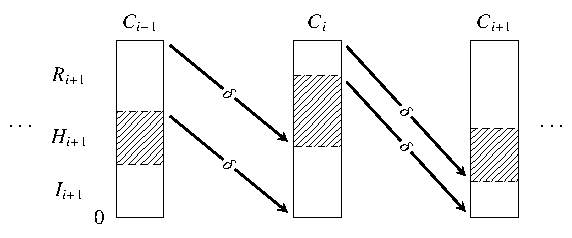
\includegraphics[width=0.54\paperwidth]{figures/Fig_001_PDF030_Book018.pdf}
  \caption{复形分解中的 $H$、$I$、$R$ 分量及微分（原书 p.18）}
  \label{fig:complex-splitting}
\end{figure}

令
\[
  h=\begin{pmatrix}0&0&0\\0&0&0\\\delta^{-1}&0&0\end{pmatrix}.
\]
容易验证，$dh$、$hd$ 和 $1-dh-hd$ 是分别投影到三个分量上的幂等元 $e_I,e_R,e_H$。此外还有
\[
  h^2=0,\qquad dhd=d,\qquad hdh=h.
\]
若 $f$ 是复形态射且 $f^{HH}=0$，则
\begin{align*}
  0=f^{HH}=e_Hfe_H
   &=f-dhf-hdf-fdh+dhfdh+hdfdh-fhd+dhfhd+hdfhd\\
   &=f-dhf-hdf-dfh+dfh+0-fhd+dhfhd+hfd\\
   &=f-dhf-fhd+dhfhd\\
   &=f-\bigl(d(hf-dhfh)+(hf-dhfh)d\bigr).
\end{align*}
因此 $f=dg+gd$，其中 $g=hf-dhfh$，所以 $f$ 零同伦。

第三条中，$\pi$ 的单射性直接由第二条得到；任意仅有 $f^{HH}$ 分量非零的映射都是复形态射，故 $\pi$ 也是满射。证明第四条时，取 $f^\dagger$ 为 $(f^{HH})^{-1}$ 在 $\pi$ 下的任意原像即可。
\end{proof}
% [Tutor Note: 这里出现的 $h^2=0$、$dhd=d$、$hdh=h$ 不是随手选出的恒等式，而是“收缩数据”的典型关系（还配上 $dh$、$hd$ 为投影、$h$ 次数为 $-1$）。第三章的同调扰动引理正是把这组关系抽象为 $\varphi\varphi^\dagger=1_B+h\mu_1^B+\mu_1^Bh$ 等条件，再据此把 $A_\infty$ 结构沿 $h$ 搬运过去；记住这套关系，后面的树形公式才看得懂。]

\subsection{范畴观点}\label{subsec:complex-category}
从更抽象的角度看，可以引入范畴 $K^\bullet(k)$。它的对象是 $k$-向量空间上的上链复形，态射为所有 $k$-线性映射：
\[
  K^\bullet(k)(C^\bullet,D^\bullet)
  =\operatorname{Hom}^\bullet(C^\bullet,D^\bullet).
\]
这个范畴实际上是微分分次范畴（简称 dg-范畴\index{dgfanchou@dg-范畴|hyperpage}）。这是一类特殊的 $k$-线性范畴，其 Hom 空间本身是上链复形，且微分满足分次 Leibniz 律：
\[
  d(f\circ g)=df\circ g+(-1)^{\deg f}f\circ dg.
\]

若要在拟同构意义下研究复形，就必须转到拟同构可逆的范畴。这可以通过考察 $HK^0(k)$ 来实现：其对象仍是 $k$-向量空间复形，Hom 空间则为 $H\operatorname{Hom}^0(C^\bullet,D^\bullet)$。由引理\ref{lem:complex-map-criterion}，这个范畴等价于分次 $k$-向量空间范畴 $\mathrm{grVECT}(k)$，其中态射是次数为 $0$ 的齐次线性映射。具体而言，函子
\[
  \pi\colon HK^0(k)\longrightarrow\mathrm{grVECT}(k),\qquad
  C^\bullet\longmapsto HC^\bullet,\quad
  f\longmapsto Hf\cong f^{HH}
\]
是范畴等价。

\begin{note}
前两节的讨论针对向量空间复形。若向量空间还带有额外结构，例如环结构或 $k$-代数 $A$ 上的模结构，这些结构通常不会在上述分解中保留下来，我们构造的拟逆也未必与额外结构相容。因此，当 $A$ 是代数时，需要调整 $HK^0(A)$ 的构造。第三章将详细讨论这一点。
\end{note}

\section{拓扑中的上同调}\label{sec:topology-cohomology}
\takeaway{$\Delta$-集是函子 $\Delta^{\mathrm{op}}\to\mathrm{Sets}$，其单纯上链复形带杯积，因而有上同调环；实现同一拓扑空间的 $\Delta$-集给出同构的上同调环（拓扑不变性），德拉姆上同调经积分映射与之拟同构；Massey 积作为高阶运算可以区分环结构区分不了的博罗米恩环。}
\subsection{粘合单形}\label{subsec:gluing-simplices}
许多拓扑空间（例如多面体）都可以由较小的部分粘合而成。若要描述一个由三角形构成的多面体，我们需要给出一组三角形、一组边和一组点；此外，还要给每个三角形指定三条边，并给每条边指定两个端点。利用 $\Delta$-集\index{deltaji@$\Delta$-集|hyperpage}，可以简洁地描述这些数据\bookcite{209}。\footnote{文献中也称之为 $\Delta$-复形\bookcite{111}。我们更愿称其为 $\Delta$-集，因为“复形”一词在本书中用于上链复形。$\Delta$-集与更常见的单纯集概念密切相关\bookcite{87}。}

\begin{definition}{严格单调递增单形范畴}{simplex-category}
严格单调递增单形范畴\index{yangedandiaodizengdanxingfanchou@严格单调递增单形范畴|hyperpage} $\Delta$ 的对象是所有集合
\[
  [n]:=\{0,\ldots,n\},\qquad n\geq 0,
\]
其态射是所有严格递增映射：
\[
  \Delta([m],[n])
  =\{\varphi\colon[m]\to[n]\mid x>y\Longrightarrow\varphi(x)>\varphi(y)\}.
\]
所有严格递增映射都是单射，并且可以由一些特殊映射——面映射\index{mianyingshe@面映射|hyperpage}——复合而成。面映射是把 $[n-1]$ 映入 $[n]$ 并跳过一个元素的单射：
\[
  \delta_i\colon[n-1]\to[n],\qquad
  x\longmapsto
  \begin{cases}
    x,&x<i,\\
    x+1,&x\geq i.
  \end{cases}
\]
\end{definition}

我们还可以用几何方式实现这个范畴。标准 $n$-单形是拓扑空间
\[
  \operatorname{Simp}_n
  :=\left\{(x_0,\ldots,x_n)\in[0,1]^{n+1}\ \middle|\ \sum_{i=0}^n x_i=1\right\}.
\]
因此 $\operatorname{Simp}_0$ 是一个点，$\operatorname{Simp}_1$ 是线段，$\operatorname{Simp}_2$ 是三角形，依此类推。
\begin{figure}[H]\centering
  \centering
  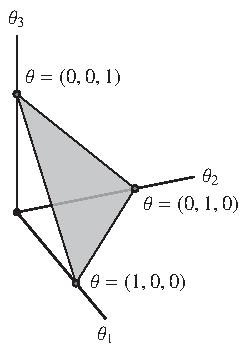
\includegraphics[width=0.46\paperwidth]{figures/Fig_002_PDF032_Book020.pdf}
  \caption{标准单形 $\operatorname{Simp}_2$ 及其顶点坐标（原书 p.20）}
  \label{fig:standard-simplex}
\end{figure}
面映射可以实现为各个面的嵌入（标准单形及其顶点坐标见图\ref{fig:standard-simplex}）：
\[
  \delta_i\colon\operatorname{Simp}_{n-1}\to\operatorname{Simp}_n,\qquad
  (x_0,\ldots,x_{n-1})\longmapsto
  (x_0,\ldots,x_{i-1},0,x_i,\ldots,x_{n-1}).
\]
几何严格单形范畴的对象是标准单形，态射由面映射生成。按构造，它与 $\Delta$ 等价。

设某个拓扑空间由点、线段、三角形等拼成，并且每个这样的对象都与一个标准 $n$-单形相对应。对于每个 $n$-单形，我们可以给出与之对应的对象所成的集合。若有映射 $\varphi\colon\operatorname{Simp}_n\to\operatorname{Simp}_m$，并且某个对象与标准 $m$-单形相对应，那么将 $\varphi$ 与这个对应复合，就会得到一个把标准 $n$-单形对应到另一个对象的映射。因此，$\varphi$ 给出从与 $m$-单形对应的对象到与 $n$-单形对应的对象的映射。这引出以下定义。

\begin{definition}{$\Delta$-集}{delta-set}
$\Delta$-集是反变函子 $S\colon\Delta\to\mathrm{Sets}$。与 $\Delta$-集相联系的几何实现\index{jiheshixian@几何实现|hyperpage}为
\[
  |S|:=\left(\coprod_i S[i]\times\operatorname{Simp}_i\right)\big/\sim,
\]
其中对每个态射 $\varphi\in\Delta$，规定
\[
  (a,\varphi(x))\sim(S(\varphi)(a),x).
\]
\end{definition}
注意，若 $\varphi$ 是面映射 $\delta_i$，上述等价关系便意味着：与 $a$ 的第 $i$ 个面对应的单形（即形如 $(S(\delta_i)(a),x)$ 的点）会与 $a$ 所对应单形中该面的嵌入（即形如 $(a,\delta_i(x))$ 的点）粘合。

\begin{example}[环面与球面的 $\Delta$-集]\label{ex:torus-sphere-delta}
\begin{enumerate}
  \item 环面 $S^1\times S^1$ 可以由函子 $S$ 实现，其中
  \[
    S[0]=\{P\},\qquad S[1]=\{\ell_0,\ell_1,\ell_2\},\qquad S[2]=\{a,b\}.
  \]
  面映射的作用为 $S(\delta_i)(\ell_j)=P$、$S(\delta_i)(a)=\ell_i$、$S(\delta_i)(b)=\ell_{2-i}$。
  \item 球面 $S^2$ 可以由函子 $S$ 实现，其中
  \[
    S[0]=\{p,q,r\},\qquad S[1]=\{\ell_0,\ell_1,\ell_2\},\qquad S[2]=\{a,b\}.
  \]
  面映射的作用满足 $S(\delta_i)(a)=\ell_i$、$S(\delta_i)(b)=\ell_i$；而对边 $\ell_j$，当 $i=1$ 时 $S(\delta_i)(\ell_j)$ 是其头端点，当 $i=0$ 时是其尾端点（见图\ref{fig:torus-sphere-delta}）。
\end{enumerate}
\end{example}
\begin{figure}[H]\centering
  \centering
  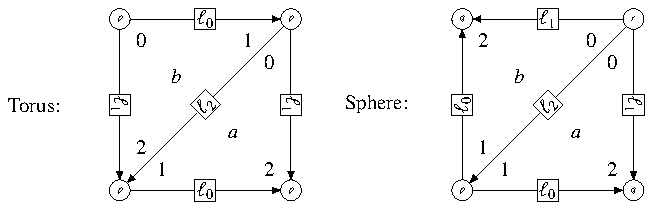
\includegraphics[width=0.82\textwidth]{figures/Fig_003_PDF033_Book021.pdf}
  \caption{环面与球面的 $\Delta$-集实现（原书 p.21）}
  \label{fig:torus-sphere-delta}
\end{figure}
不同的 $\Delta$-集可能给出同胚的拓扑空间。为了对此加以控制，我们希望定义只依赖于拓扑实现的拓扑不变量。

\subsection{单纯上同调}\label{subsec:simplicial-cohomology}
\begin{definition}{$\Delta$-集的单纯上同调}{simplicial-cohomology}
设 $S$ 是一个 $\Delta$-集，$k$ 是一个域。定义向量空间上链复形
\[
  C_\Delta^i(S,k):=\mathrm{Sets}(S[i],k),
\]
其微分为
\[
  df=\sum_j(-1)^j f\circ\delta_j.
\]
容易验证 $d^2=0$。复形 $C_\Delta^\bullet(S,k)$ 的上同调称为 $S$ 的单纯上同调\index{danchunshangtongdiao@单纯上同调|hyperpage}，记为 $H^\bullet(S,k)$。
\end{definition}

\begin{note}
这一构造可以分成两步：
\begin{enumerate}
  \item 将 $S$ 与函子 $\mathrm{Sets}(-,k)$ 复合，把它变成左 $\Delta$-模 $M\colon\Delta\to\mathrm{VECT}(k)$；
  \item 将左 $\Delta$-模 $M$ 变成上链复形 $M^\bullet$，其中 $M^i=M[i]$，且 $d=\sum_j(-1)^jM(\delta_j)$。
\end{enumerate}
在某些情形下，$\Delta$-集本身已经带有 $\Delta$-模结构，此时可以略去第一步。
\end{note}

如何理解单纯上链复形？注意，$f\in C_\Delta^i(S,k)$ 把每个 $i$-单形对应到一个数，可以把它想成流经该单形的流量。从这个角度看，$df$ 衡量流经每个 $(i+1)$-单形边界的流入与流出之差。若 $df=0$，则流量不会在某个 $(i+1)$-单形中累积，因此它表示一个闭流。若 $\Delta$-集有一个洞（例如缺少某个 $(i+1)$-单形），闭流就可能在那个缺失的单形处累积。这类流却不会是恰当的，因而会在上同调中留下非零类。因此，可以说 $S$ 的上同调测量了拓扑空间 $|S|$ 中的洞。
\begin{figure}[H]\centering
  \centering
  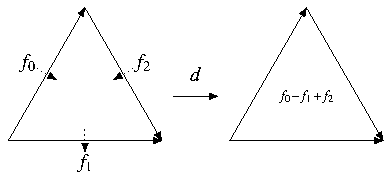
\includegraphics[width=0.48\paperwidth]{figures/Fig_004_PDF034_Book022.pdf}
  \caption{单纯上链中的流量与边界微分（原书 p.22）}
  \label{fig:cochain-flow}
\end{figure}

\begin{definition}{杯积}{cup-product}
上链复形 $C_\Delta^\bullet(S,k)$ 带有自然乘积。若 $f\in C_\Delta^p(S,k)$、$g\in C_\Delta^q(S,k)$，定义杯积\index{beiji@杯积|hyperpage} $f\smile g\in C_\Delta^{p+q}(S,k)$ 为
\[
  (f\smile g)(a):=f(S(\iota_p)(a))\cdot g(S(\upsilon_q)(a)),
\]
其中 $\iota_p$ 是包含映射 $[p]=\{0,\ldots,p\}\subset\{0,\ldots,p+q\}=[p+q]$，而
\[
  \upsilon_q\colon[q]\to[p+q],\qquad x\longmapsto x+p.
\]
可以验证，这个乘积满足结合律和分次 Leibniz 律：
\[
  d(f\smile g)=df\smile g+(-1)^p f\smile dg.
\]
因此，上同调上也定义了乘积：若 $df=dg=0$，则 $d(f\smile g)=0$，所以闭元的乘积仍是闭元。此外，
\[
  (f+dh)\smile g=f\smile g+d(h\smile g),
\]
因此给 $f$ 加上恰当元不会改变乘积的上同调类。
% [Tutor Note: 原书此处把末式印成 $(f+dh)\smile g=f\smile g-d(h\smile g)$，符号有误：由 $d(h\smile g)=dh\smile g+(-1)^{|h|}h\smile dg$ 与 $dg=0$ 得 $d(h\smile g)=dh\smile g$，故应为加号（译文已按加号排）。另外注意两处符号的不同来源：Leibniz 律里的 $(-1)^p$ 来自 $f$ 的次数 $p$，而末式的成立只用 $dg=0$，$df=0$ 仅用于保证 $[f]$ 是上同调类。]
\end{definition}

\begin{definition}{上同调环}{cohomology-ring}
配备杯积的空间 $HC_\Delta^\bullet(S,k)$ 称为 $S$（系数取 $k$）的上同调环\index{shangtongdiaohuan@上同调环|hyperpage}，记作 $H^\bullet(S,k)$。
\end{definition}

\begin{example}[环面的上同调环]\label{ex:torus-cohomology-ring}
利用例\ref{ex:torus-sphere-delta}中的 $\Delta$-集计算环面的上同调环。令 $P$ 表示在所有顶点上取 $1$ 的常函数；$L_0,L_1,L_2,A,B$ 分别表示在 $\ell_0,\ell_1,\ell_2,a,b$ 上取 $1$、在其余顶点上取 $0$ 的函数。微分满足
\[
  dP=dA=dB=0,\qquad dL_i=(-1)^{i+1}(A+B),
\]
因此上同调的一组基为 $[P]$、$[L_0+L_1]$、$[L_2+L_1]$ 和 $[A]=-[B]$。所有单形的角点都是 $p$，故 $P\smile X=X$。此外，对 $a$ 有 $S(\iota_1)(a)=\ell_2$、$S(\upsilon_1)(a)=\ell_0$；对 $b$ 则相反，即 $S(\iota_1)(b)=\ell_0$、$S(\upsilon_1)(b)=\ell_2$。因此
\[
  L_0\smile L_2=B,\qquad L_2\smile L_0=A,
\]
而 $L_i$ 之间的其他乘积均为零。由此得到上同调环
\[
  HC_\Delta^\bullet(S,k)\cong
  \frac{k\langle\xi,\eta\rangle}{\langle\xi\eta+\eta\xi,\xi^2,\eta^2\rangle},
\]
其中
\[
  1=[P],\qquad \xi=[L_0+L_1],\qquad
  \eta=[L_2+L_1],\qquad
  \xi\eta=[B]=-[A]=-\eta\xi.
\]
\end{example}

几何实现同胚的不同 $\Delta$-集会给出不同的上链复形，但其上同调环相同。证明这一点的一种方法，是把它们与只依赖空间 $X=|S_1|=|S_2|$ 的上同调环联系起来。

\begin{definition}{奇异上同调环}{singular-cohomology}
对拓扑空间 $X$，定义 $\Delta$-集 $X$，其 $i$-单形是从 $\operatorname{Simp}_i$ 到 $X$ 的所有连续映射：
\[
  X[i]=\mathrm{Top}(\operatorname{Simp}_i,X),\qquad
  X[\delta_i](f)=f\circ\delta_i.
\]
上同调环 $HC_\Delta^\bullet(X,k)$ 称为 $X$ 的奇异上同调环\index{qiyishangtongdiaohuan@奇异上同调环|hyperpage}，记作
\[
  H^\bullet(X,k):=HC_\Delta^\bullet(X,k).
\]
\end{definition}

\begin{theorem}{拓扑不变性}{topological-invariance}
若 $S$ 是一个几何实现为 $X=|S|$ 的 $\Delta$-集，则
\[
  HC_\Delta^\bullet(S,k)\cong H^\bullet(X,k)
\]
作为分次环同构。
\end{theorem}
\begin{proof}[证明思路]
单纯复形 $S$ 自然嵌入到 $X$ 中，从而给出一个限制映射
\[
  C_\Delta^\bullet(X,k)\longrightarrow C_\Delta^\bullet(S,k),
\]
它是 dg-代数态射。可以证明该映射是拟同构，因此在上同调层面诱导出分次环同构。更多信息见\bookcite{111}。
\end{proof}

\begin{note}
设两个 $\Delta$-集 $S_1,S_2$ 满足 $|S_1|\cong|S_2|=X$，则有如下图式，其中两条实线箭头是环的拟同构：
\begin{figure}[H]\centering
  \centering
  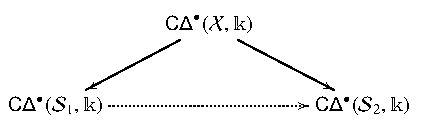
\includegraphics[width=0.43\paperwidth]{figures/Fig_005_PDF036_Book024.pdf}
  \caption{由同一拓扑空间诱导的上链复形之间的拟同构（原书 p.24）}
  \label{fig:topological-quasi-isomorphisms}
\end{figure}
由引理\ref{lem:complex-map-criterion}，存在一个使图交换的向量空间拟同构：将第二个投影与第一个投影的拟逆复合即可。遗憾的是，这个拟同构一般不是环的拟同构。
\end{note}

\subsection{德拉姆上同调}\label{subsec:de-rham-cohomology}
设 $M$ 是光滑、紧致、可定向流形。回忆一下，$k$-形式是反对称积 $\Lambda^kT^*M$ 的一个截面。在局部坐标中，可以写成
\[
  \omega=\sum_{i_1<\cdots<i_k}
  \omega_{i_1\ldots i_k}\,dx_{i_1}\wedge\cdots\wedge dx_{i_k},
\]
其微分为
\[
  d\omega=
  \sum_{i_1<\cdots<i_k}\sum_j
  \frac{\partial\omega_{i_1\ldots i_k}}{\partial x_j}
  \,dx_j\wedge dx_{i_1}\wedge\cdots\wedge dx_{i_k},
\]
这里采用约定 $dx_i\wedge dx_j=-dx_j\wedge dx_i$。$k$-形式空间记作 $\Omega^k(M)$。

\begin{definition}{德拉姆复形与德拉姆上同调}{de-rham-complex}
三元组 $(\Omega^\bullet(M),d,\wedge)$ 构成一个 dg-代数，称为德拉姆复形\index{delamufuxing@德拉姆复形|hyperpage}。这个复形的上同调环称为德拉姆上同调\index{delamushangtongdiao@德拉姆上同调|hyperpage}：
\[
  H_{\mathrm{dR}}^\bullet(M):=H\Omega^\bullet(M).
\]
\end{definition}
若 $f\colon\operatorname{Simp}_k\to M$ 是光滑映射，则可以拉回任意 $k$-形式 $\omega\in\Omega^k(M)$ 并对其积分。若 $S$ 是满足 $|S|\cong M$ 的 $\Delta$-集，这一过程给出映射
\[
  \varphi\colon\Omega^\bullet(M)\longrightarrow C_\Delta^\bullet(S,\mathbb R),
  \qquad \omega\longmapsto\bigl(a\longmapsto\int_a\omega\bigr),
\]
其中 $\int_a$ 表示在 $|S|\cong M$ 中嵌入的单形 $\{a\}\times\operatorname{Simp}_k$ 上积分。斯托克斯定理表明该映射是复形态射：
\[
  \varphi(d\omega)(a)=\int_a d\omega
  =\int_{\partial a}\omega
  =\sum_i\pm\int_{\delta_i a}\omega
  =d\varphi(\omega)(a).
\]
该映射还与乘积相容，因此有如下定理。其证明和更多细节可参见\bookcite{45}。

\begin{theorem}{德拉姆定理}{de-rham-theorem}
映射 $\varphi\colon\Omega^\bullet(M)\to C_\Delta^\bullet(S,\mathbb R)$ 是拟同构。
\end{theorem}

\subsection{Massey 积}\label{subsec:massey-products}
从 $C_\Delta^\bullet(S,\mathbb R)$ 或 $\Omega^\bullet(M)$ 上的乘积过渡到上同调上的乘积，往往会损失信息。为弥补这一点，可以引入称为 Massey 积\index{masseyji@Massey 积|hyperpage}的高阶乘积。Massey 积是一种构造新上同调类的方法：给定一列满足某些附加条件的上同调类，可以由它们得到新的上同调类。

三元 Massey 积的构造如下。取三个上同调类 $[u],[v],[w]$，并假设 $[u\smile v]=[v\smile w]=0$。这意味着存在元素 $s,t\in C_\Delta^\bullet(S,k)$，使得
\[
  u\smile v=ds,\qquad v\smile w=dt.
\]
利用 Leibniz 律可得
\[
  d(u\smile t)=du\smile t\pm u\smile dt=\pm u\smile v\smile w,
\]
\[
  d(s\smile w)=ds\smile w\pm s\smile dw=u\smile v\smile w.
\]
因此，选取适当的符号后，有 $d(u\smile t\pm s\smile w)=0$，于是可以考察上同调类 $[u\smile t\pm s\smile w]$。注意其定义取决于 $s,t$ 的选择；Massey 积 $\langle[u],[v],[w]\rangle$ 定义为改变 $s,t$ 后所有可能得到的上同调类所成的集合。
% [Tutor Note: 三个要点：其一，$\langle[u],[v],[w]\rangle$ 一般是一个集合而非单个类（只有当它只含一个元素时才说“良定义”），所以博罗米恩环那个例子的结论写成“含有非零类/只含零类”。其二，两处的 $\pm$ 必须取相容的符号，最终类才闭；不同 $s,t$ 给出的类相差 $\pm$ 恰当项。其三，这一“选 $s,t$ 再取类”的不定性，正是第三章 $A_\infty$ 语言中 $\mu_3$ 只定义到同伦（或到 $\pm$）的原因。]

\begin{example}[博罗米恩环与 Massey 积]\label{ex:borromean-massey}
设 $S$ 是一个实现单位立方体 $[0,1]^3$ 的 $\Delta$-集。令 $\gamma_1,\gamma_2,\gamma_3\colon S^1\to(0,1)^3$ 是嵌入单位立方体的三条两两不交的圆周，并假设每个单形至多与其中一条曲线相交，且交集只是一段区间。定义 $S_\gamma$ 为由所有与 $\gamma_i$ 不相交的单形构成的 $\Delta$-集。

固定单位立方体中以 $\gamma_i$ 为边界的圆盘 $D_i$，并定义 $\lambda_i\in H^1(S_\gamma,k)$ 如下：
\[
  \text{对每个 }a\in S[1],\qquad
  \lambda_i(a)=
  \begin{cases}
    1,&a\text{ 沿正向穿过 }D_i,\\
    -1,&a\text{ 沿负向穿过 }D_i,\\
    0,&a\text{ 不穿过 }D_i.
  \end{cases}
\]
虽然这个定义依赖于 $D_i$ 的选择，但其上同调类只依赖于 $\gamma_i$。

若 $\gamma_i$ 与 $\gamma_j$ 互不链接，则可以证明 $\lambda_i\smile\lambda_j=0\in H^2(S_\gamma,k)$；若它们像霍普夫链环那样相互套链，则 $\lambda_i\smile\lambda_j\neq0$。
\begin{figure}[H]\centering
  \centering
  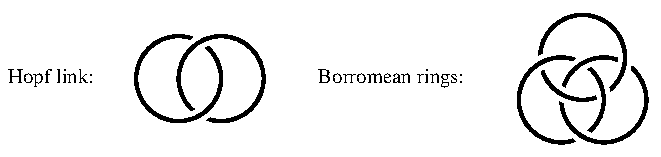
\includegraphics[width=0.62\paperwidth]{figures/Fig_006_PDF038_Book026.pdf}
  \caption{霍普夫链环与博罗米恩环（原书 p.26）}
  \label{fig:hopf-borromean}
\end{figure}
博罗米恩环是嵌入三维空间中的三条环：忽略其中任意一条，另外两条都可以在不相交的情况下分开；但三条环整体却不能分开。因此，对所有 $i,j$，都有 $\lambda_i\smile\lambda_j=0$，这正是可以定义 Massey 积的情形。Massey 在\bookcite{171}中计算得出，$\langle\lambda_1,\lambda_2,\lambda_3\rangle$ 含有一个非零上同调类；而对三条完全没有相互链接的圆周进行同样计算时，$\langle\lambda_1,\lambda_2,\lambda_3\rangle$ 只含零类。
\end{example}

上同调环的环结构无法区分博罗米恩环与彼此松散的三条环，但 Massey 积可以。在下一章中，我们将看到一种增强上同调环的方式，把这些高阶乘积也纳入其中。

\section{代数中的上同调}\label{sec:algebra-cohomology}
把复杂空间切分为较简单的部分并研究它们如何粘合起来，这一思想可以推广到数学的许多领域。本节将在代数的表示论中考察这一思路。

\takeaway{自由分解把模的问题化为自由模复形的计算：比较定理保证提升存在且在同伦意义下唯一，故 $\operatorname{Ext}$ 群与 Ext 环不依赖分解的选择；Koszul 分解把 $\operatorname{Ext}^\bullet_A(S,S)$ 算成与生成元、关系对偶的代数，而乘法只能恢复关系的二次部分。}

\subsection{分解}\label{subsec:resolutions}
设 $A$ 是 $k$ 上的代数，$M$ 是右 $A$-模。若 $M$ 由集合 $S^0$ 生成，就可以从自由模构造一个到 $M$ 的满射：
\[
  M\longleftarrow\bigoplus_{m\in S^0}A=:P^0.
\]
这个映射的核有一个生成集 $S^1$，因而可以构造映射
\[
  P^0\longleftarrow\bigoplus_{m\in S^1}A=:P^{-1}.
\]
如此继续下去（并令 $i>0$ 时 $P^i=0$），最终得到一个由自由模构成的上链复形 $P^\bullet$。按构造，该复形的同调在次数 $0$ 等于 $M$，其他次数均为零。

\begin{definition}{自由分解}{free-resolution}
右 $A$-模 $M$ 的自由分解\index{ziyoufenjie@自由分解|hyperpage}，是一个由自由 $A$-模构成的复形 $P^\bullet$，满足 $HP^\bullet=M^\bullet$；这里 $M^\bullet$ 表示仅在次数 $0$ 有 $M$、其他次数均为零的复形。
\end{definition}
注意，这一构造并不能给出唯一的自由分解，因为它取决于生成元的选择。不过可以证明，$M$ 的任意两个自由分解都拟同构。进一步还有以下引理。

\begin{theorem}{比较定理}{comparison-theorem}
若 $\varphi\colon M\to N$ 是态射，且 $P^\bullet,Q^\bullet$ 分别是 $M,N$ 的自由分解，则存在复形态射 $\bar\varphi$，使其在同调上诱导的态射为 $\varphi$。这个提升在相差同伦的意义下唯一。
\end{theorem}
\begin{proof}[证明思路]
思路是逐步构造 $\bar\varphi$：因为 $Q^0\to N$ 是满射，可以找到 $q_i\in Q^0$，使它们分别映到 $P^0\to M\to N$ 下各生成元的像。将 $P^0$ 的生成元映到这些 $q_i$，就得到 $P^0$ 上的提升 $\bar\varphi^0$。
\begin{figure}[H]\centering
  \centering
  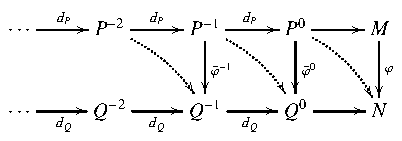
\includegraphics[width=0.52\paperwidth]{figures/Fig_007_PDF040_Book028.pdf}
  \caption{自由分解之间对模态射的逐步提升（原书 p.28）}
  \label{fig:comparison-theorem-lift}
\end{figure}
现在考察 $P^{-1}$ 的生成元经 $\bar\varphi^0d_P$ 后的像。由提升性质，这些像落在 $Q^0\to N$ 的核中，因此可以找到它们在 $d_Q$ 下的原像。把 $P^{-1}$ 的生成元映到这些原像，就得到 $\bar\varphi^{-1}$。随后考察 $P^{-2}$ 的生成元，并重复同一过程，最终构造出整个 $\bar\varphi$。唯一性可用类似论证证明；见\bookcite[定理 2.2.6]{253}。
\end{proof}
% [Tutor Note: “唯一性可用类似论证证明”省掉的正是同伦 $s$ 的构造，其归纳步骤是：在次数 $0$，差 $\bar\psi^0-\bar\varphi^0$ 是闭的且落在 $\ker(Q^0\to N)=\operatorname{im}d_Q$ 中，用 $P^0$ 的自由性提升得到 $s^0$ 使 $\bar\psi^0-\bar\varphi^0=d_Qs^0$；随后考察 $\bar\psi^{i}-\bar\varphi^{i}-s^{i-1}d_P$（$i<0$），它仍是闭的且落在 $\operatorname{im}d_Q$ 中，再提升一次。每一步都依赖 $P^\bullet$ 由自由（或投射）模构成，这就是定理必须对这类分解陈述的原因。]
特别地，对 $\varphi$ 取恒等态射 $1_M$，便得到 $M$ 的任意一对自由分解 $P^\bullet,Q^\bullet$ 之间的拟同构。

\begin{note}
除了自由分解，也可以使用更一般的投射分解，其中每个分量都是投射 $A$-模（即自由模的直和项）。和自由分解一样，模的任意两个投射分解都拟同构。
\end{note}

\subsection{Ext 群}\label{subsec:ext-groups}
设有两个 $A$-模 $M,N$，其分解分别为 $P^\bullet,Q^\bullet$。在这两个复形之间可以考察 Hom 复形
\[
  \operatorname{Hom}_A^j(P^\bullet,Q^\bullet)
  :=\bigoplus_i\operatorname{Hom}_A(P^i,Q^{i+j}),
  \qquad
  df=d_Qf-(-1)^{\deg f}fd_P.
\]
尽管这个复形取决于具体的分解，其上同调只依赖于 $M,N$。对零次上同调而言，这直接由定理\ref{thm:comparison-theorem}推出：
\[
  H\operatorname{Hom}_A^0(P^\bullet,Q^\bullet)
  \cong\operatorname{Hom}_A(M,N).
\]
其他次数的上同调则由同一模的任意自由分解都拟同构这一事实推出。

\begin{definition}{Ext 群}{ext-groups}
设 $M$ 是带有自由分解 $P^\bullet$ 的 $A$-模，$N$ 是带有自由分解 $Q^\bullet$ 的 $A$-模。定义第 $i$ 个 Ext 群\index{extqun@Ext 群|hyperpage}为
\[
  \operatorname{Ext}_A^i(M,N):=
  H\operatorname{Hom}_A^i(P^\bullet,Q^\bullet).
\]
\end{definition}

\begin{note}
由比较定理可知，这一定义不依赖于 $M,N$ 的自由分解选择。此外，利用与定理\ref{thm:comparison-theorem}类似的论证，也可以证明
\[
  H\operatorname{Hom}_A^i(P^\bullet,Q^\bullet)
  =H\operatorname{Hom}_A^i(P^\bullet,N).
\]
这往往能大大简化 $\operatorname{Ext}_A^i(M,N)$ 的计算。
\end{note}

\begin{example}[一元多项式代数上的 Ext 群]\label{ex:ext-polynomial-one-variable}
考虑代数 $k[X]$，令 $S^\lambda$ 为一维简单模，其中 $X$ 的作用是乘以 $\lambda$。这个模有一个分解
\[
  P_\lambda^\bullet:=
  \left(k[X]\xrightarrow{\,X-\lambda\,}k[X]\right),
\]
因而复形 $\operatorname{Hom}_{k[X]}^\bullet(P_\lambda^\bullet,P_\mu^\bullet)$ 为
\[
  k[X]\xrightarrow{\binom{X-\mu}{-X+\lambda}}
  k[X]^{\oplus2}\xrightarrow{\left(\begin{smallmatrix}X-\lambda&X-\mu\end{smallmatrix}\right)}
  k[X],
\]
其中中间项次数为 $0$。由于 $k[X]$ 是整环，$\operatorname{Ext}^{-1}(S^\lambda,S^\mu)=0$。这是一般现象：对任意代数和模，都有 $\operatorname{Ext}_A^{<0}(M,N)=0$。

至于 $\operatorname{Ext}^1$，答案取决于 $\lambda,\mu$。$d_0$ 的像是理想 $(X-\lambda,X-\mu)\subset k[X]$。若 $\lambda\neq\mu$，该理想就是整个环，因此 $\operatorname{Ext}^1(S^\lambda,S^\mu)=0$；若 $\lambda=\mu$，则
\[
  \operatorname{Ext}^1(S^\lambda,S^\lambda)
  =\frac{k[X]}{(X-\lambda)}=k.
\]
$\operatorname{Ext}_A^1(M,N)$ 还有一个很自然的表示论解释。
\end{example}

\begin{definition}{扩张及其等价}{module-extension}
一个扩张\index{kuozhang@扩张|hyperpage}是短正合列
\[
  N\lhook\joinrel\longrightarrow E\twoheadrightarrow M.
\]
若两个扩张之间存在如下交换图，则称它们等价：
\begin{figure}[H]\centering
  \centering
  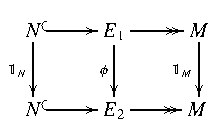
\includegraphics[width=0.46\paperwidth]{figures/Fig_008_PDF041_Book029.pdf}
  \caption{两个等价扩张之间的交换图（原书 p.29）}
  \label{fig:equivalent-extensions}
\end{figure}
\end{definition}

\begin{theorem}{Ext 群分类扩张}{ext-classifies-extensions}
向量空间 $\operatorname{Ext}_A^1(M,N)$ 按等价分类从 $M$ 到 $N$ 的所有扩张。特别地，若 $\operatorname{Ext}_A^1(M,N)=0$，则每个短正合列
\[
  N\lhook\joinrel\longrightarrow E\twoheadrightarrow M
\]
都分裂：$E\cong M\oplus N$。
\end{theorem}
\begin{proof}[证明思路]
给定一个扩张，可以把 $M$ 上的恒等映射沿着分解逐步提升，从而构造一个态射：
\begin{figure}[H]\centering
  \centering
  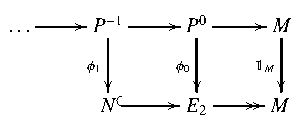
\includegraphics[width=0.40\paperwidth]{figures/Fig_009_PDF042_Book030.pdf}
  \caption{由扩张得到 Ext 群中的元素（原书 p.30）}
  \label{fig:extension-ext-class}
\end{figure}
这会诱导出一个映射类 $[\varphi_1]\in\operatorname{Ext}_A^1(M,N)$。可以证明这个对应是同构；证明见\bookcite{253}的定理 3.4.3。若 $\operatorname{Ext}_A^1(M,N)=0$，则每个扩张都与平凡扩张同构，因而分裂。
\end{proof}

\begin{example}[一个非平凡扩张]\label{ex:nonsplit-extension}
在前面的例子中，可以直接验证短正合列
\[
  \frac{k[X]}{(X-\lambda)}
  \lhook\joinrel\xrightarrow{\ X-\lambda\ }
  \frac{k[X]}{(X-\lambda)^2}
  \twoheadrightarrow
  \frac{k[X]}{(X-\lambda)}
\]
不分裂；它对应于非零 Ext 群中的一个元素。
\end{example}

\subsection{Ext 环}\label{subsec:ext-ring}
给定 $A$-模 $M$ 及其自由分解 $P^\bullet$，Hom 空间 $\operatorname{Hom}_A^\bullet(P^\bullet,P^\bullet)$ 带有由态射复合给出的环结构。由于这一环结构与微分相容，它也在上同调上诱导环结构。因此得到分次环 $\operatorname{Ext}_A^\bullet(M,M)$，并且它不依赖于分解的选择。本节将考察若干特殊情形下 Ext 环的结构。

\begin{example}[对偶数环]\label{ex:dual-numbers-ext}
最简单的情形是 $A=k[X]$、$M=k[X]/(X)$。此时 $M$ 有分解 $F^\bullet=A\xrightarrow{X}A$，并且
\[
  \operatorname{Hom}_A^\bullet(F^\bullet,F^\bullet)=\operatorname{Mat}_2(A),
  \qquad
  df=\begin{pmatrix}0&X\\0&0\end{pmatrix}f
       -(-1)^{\deg f}f\begin{pmatrix}0&X\\0&0\end{pmatrix}.
\]
其同调是二维分次向量空间
\[
  k\begin{pmatrix}1&0\\0&1\end{pmatrix}
  \oplus k\begin{pmatrix}0&1\\0&0\end{pmatrix}
  =:k\iota\oplus k\xi.
\]
生成元 $\xi$ 的次数为 $1$，且 $\xi^2=0$，故
\[
  \operatorname{Ext}_A^\bullet(M,M)\cong\frac{k[\xi]}{\langle\xi^2\rangle}.
\]
这个环称为对偶数环\index{duioushuhuan@对偶数环|hyperpage}。
\end{example}

\begin{example}[平面原点的 Ext 环]\label{ex:ext-polynomial-two-variables}
考察 $A=k[X,Y]$，并令 $S=k[X,Y]/(X,Y)$ 为 $X,Y$ 均平凡作用的简单模。此时有一个很好的分解，称为 Koszul 分解：
\[
  K^\bullet:=A\xrightarrow{\binom{Y}{-X}}A^{\oplus2}
  \xrightarrow{\left(\begin{smallmatrix}X&Y\end{smallmatrix}\right)}A.
\]
结合前面“Ext 群与自由分解的选取无关”这一结论，可知 Ext 群为
\[
  \operatorname{Ext}_A^\bullet(S,S)
  =H\left(S\xrightarrow{\,0\,}S^{\oplus2}\xrightarrow{\,0\,}S\right)
  =k\iota\oplus(k\xi\oplus k\eta)\oplus k\rho,
\]
其中 $\iota,\xi,\eta,\rho$ 依次对应分解中的四个 $A$ 分量，都是把 $a$ 送到 $a\bmod(X,Y)$ 的映射 $A\to S$。我们可以把这四个映射提升为复形态射 $K^\bullet\to K^\bullet$。显然，$\iota$ 提升为恒等映射，而 $\xi,\eta$ 的提升分别如下：
\begin{figure}[H]\centering
  \centering
  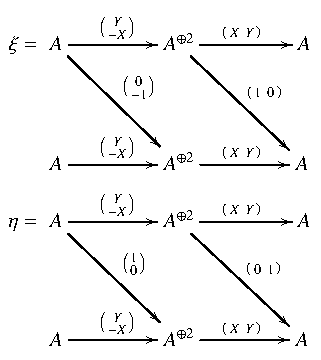
\includegraphics[width=0.70\paperwidth]{figures/Fig_010_PDF043_Book031.pdf}
  \caption{生成元 $\xi$ 与 $\eta$ 的复形态射提升（原书 p.31）}
  \label{fig:ext-generators-lifts}
\end{figure}
这些图不是交换图而是反交换图，因为 $\deg\xi=\deg\eta=1$。它们的复合为
\begin{figure}[H]\centering
  \centering
  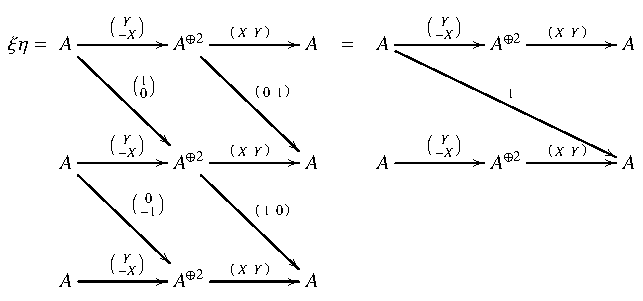
\includegraphics[width=0.70\paperwidth]{figures/Fig_011_PDF043_Book031.pdf}
  \caption{生成元 $\xi$ 与 $\eta$ 的复合（原书 p.31）}
  \label{fig:ext-product-lifts}
\end{figure}
它给出 $\rho$ 的一个提升，而反方向的复合给出 $-\rho$ 的提升。$\xi$ 与自身的复合为零，$\eta$ 与自身的复合也为零。因此
\[
  \operatorname{Ext}_A^\bullet(S,S)
  \cong\frac{k\langle\xi,\eta\rangle}
  {\langle\xi^2,\eta^2,\xi\eta+\eta\xi\rangle}.
\]
% [Tutor Note: $\xi,\eta$ 都是奇次类，而 Ext 环按 Koszul 符号约定分次交换：$\xi\eta=(-1)^{|\xi||\eta|}\eta\xi=-\eta\xi$，所以 $\xi\eta+\eta\xi=0$ 是由次数决定的，与提升的具体取法无关（多项式环情形那条定理中外代数 $\Lambda_n$ 的全部关系都由此而来）。但像“反方向复合给出 $-\rho$ 的提升”“$\xi$ 自乘为零”这类具体结论，仍须把提升按 $K^\bullet$ 的分次逐块相乘、逐块核对符号才能得到，不能只凭分次交换性断言。]
\end{example}

\begin{theorem}{多项式代数的 Ext 环}{polynomial-ext-exterior}
若 $A=k[X_1,\ldots,X_n]$，且 $S=k[X_1,\ldots,X_n]/(X_1,\ldots,X_n)$，则
\[
  \operatorname{Ext}_A^\bullet(S,S)
  \cong
  \frac{k\langle\xi_1,\ldots,\xi_n\rangle}
  {\langle\xi_i\xi_j+\xi_j\xi_i\mid 1\leq i,j\leq n\rangle}
  =:\Lambda_n.
\]
这个代数也称为具有 $n$ 个变量的外代数\index{waidaishu@外代数|hyperpage}\bookcite[第 4.5 节]{253}。
\end{theorem}

我们可以把这一构造推广到更复杂的代数。设代数具有如下形式：
\[
  A=\frac{k\langle X_1,\ldots,X_k\rangle}{\langle r_1,\ldots,r_l\rangle},
\]
其中每个关系都是次数至少为 $2$ 的单项式的线性组合。记 $\langle X_1,\ldots,X_k\rangle$ 为 $X$，记 $\langle r_1,\ldots,r_l\rangle$ 为 $R$，则条件可写作
\[
  R\subset X^2.
\]
此外，假设 $r_i$ 在向量空间 $R/(XR+RX)$ 中构成一组基。若满足此条件，就称 $k\langle X_1,\ldots,X_k\rangle/\langle r_1,\ldots,r_l\rangle$ 是 $A$ 的极小表现\index{jixiaobiaoxian@极小表现|hyperpage}。与多项式环的情形类似，可以考察简单模 $S=A/X$ 及其 Ext 环。

\begin{lemma}{极小表现的自由分解}{minimal-presentation-resolution}
上述模 $S$ 有一个自由分解，其开头部分为
\[
  K^\bullet:=\cdots\longrightarrow A^{\oplus l}
  \xrightarrow{(\partial_i r_j)_{ij}}A^{\oplus k}
  \xrightarrow{(X_1\ \cdots\ X_k)}A,
\]
其中 $\partial_i$ 是一个 $k$-线性算子：若单项式 $X_{s_1}\cdots X_{s_u}$ 的首项为 $X_i$，则
\[
  \partial_i(X_{s_1}\cdots X_{s_u})=X_{s_2}\cdots X_{s_u};
\]
否则结果为零。
\end{lemma}
\begin{proof}[证明思路]
先注意，算子 $\partial_i$ 会从每个关系单项式的首部移除一个 $X_i$，并删去所有无法如此处理的单项式。因此，对每个 $f\in k\langle X_1,\ldots,X_k\rangle$，都有恒等式
\[
  f=\sum_iX_i(\partial_i f).
\]
由于 $X_i$ 是代数 $A$ 的生成元，映射 $A^{\oplus k}\xrightarrow{(X_1\ \cdots\ X_k)}A$ 是满射。现在设 $f_i\in k\langle X_1,\ldots,X_k\rangle$ 满足 $\sum_iX_if_i=r\in R$。可以将 $r$ 写成
\[
  r=\sum_j r_jg_j+u,
\]
其中 $u$ 是形如 $vr_jw$ 的表达式的线性组合，且 $v$ 的次数至少为 $1$。对 $r$ 作用 $\partial_i$，得到
\[
  f_i=\partial_i r=\sum_j(\partial_i r_j)g_j+\partial_i u.
\]
最后一项在 $A$ 中为零，因为 $\partial_i$ 不会作用到关系内部。在 $A$ 中，因而有 $f_i=\sum_j(\partial_i r_j)g_j$，向量 $(f_i)_i$ 是 $(\partial_i r_j)_i$ 的线性组合。因此，分解中的第二个映射覆盖第一个映射的核。其余映射可照常构造：找出 $d_i$ 的核的生成元，再取一个自由模映到这些生成元上。
\end{proof}

这个分解使我们能够描述 Ext 代数的重要一部分及其乘法结构。
\begin{theorem}{Ext 环的低次部分}{ext-low-degrees}
若 $A,S$ 如上，则
\[
  \operatorname{Ext}_A^0(S,S)=k,\qquad
  \operatorname{Ext}_A^1(S,S)=k^{\oplus k}
    =k\xi_1\oplus\cdots\oplus k\xi_k,\qquad
  \operatorname{Ext}_A^2(S,S)=k^{\oplus l}
    =k\rho_1\oplus\cdots\oplus k\rho_l.
\]
并且 $\operatorname{Ext}_A^\bullet(S,S)$ 中的乘积满足如下关系：
\[
  \xi_i\xi_j=\sum_u\lambda^u_{ij}\rho_u
  \quad\Longleftrightarrow\quad
  r_u=\sum_{ij}\lambda^u_{ij}X_jX_i+\text{高次项}.
\]
\end{theorem}
\begin{proof}[证明思路]
将自由分解 $K^\bullet$ 映到 $S$，得到
\[
  S\longrightarrow S^{\oplus k}\longrightarrow S^{\oplus l}
  \longrightarrow\cdots,
\]
其中所有映射均为零。第一个映射为零，是因为生成元在 $S$ 上都作用为零；第二个为零，是因为当 $R\subset\langle X_1,\ldots,X_k\rangle^2$ 时，没有任何 $(\partial_i r_j)$ 含常数项；第三个为零，是因为 $r_i$ 构成 $R/(XR+RX)$ 的一组基。

由于这些映射都为零，
\[
  \operatorname{Ext}_A^1(S,S)=\operatorname{Hom}(A^{\oplus k},S)\cong k^{\oplus k}.
\]
可以选择基元素 $\xi_i$，令它把 $A^{\oplus k}$ 第 $i$ 个直和项中的 $1$ 映到 $1\in S$。这组基与生成元 $X_1,\ldots,X_k$ 对偶。类似地，基 $\rho_1,\ldots,\rho_l$ 属于
\[
  \operatorname{Ext}_A^2(S,S)=\operatorname{Hom}(A^{\oplus l},S)\cong k^{\oplus l},
\]
并与关系 $r_1,\ldots,r_l$ 对偶。结构常数的计算与多项式环情形完全类似。更多细节参见\bookcite{168}。
\end{proof}

\begin{note}
这个定理说明，我们可以从 Ext 环的乘法中恢复关系的二次部分。自然会问：能否进一步恢复三次或更高次部分？单靠乘法做不到；不过上述结果似乎暗示，我们需要定义三重乘积来恢复三次部分、四重乘积来恢复四次部分，依此类推。下一章将看到，确实可以这样做。
\end{note}

\begin{note}
在几何上同调一节中，我们发现环面的上同调环是外代数
\[
  \Lambda_2=\frac{\mathbb C\langle\xi,\eta\rangle}
  {\langle\xi^2,\eta^2,\xi\eta+\eta\xi\rangle};
\]
在代数上同调一节中，我们又发现同一个环可以解释为简单 $\mathbb C[X,Y]$-模的 Ext 环。两个看似无关的对象产生同一个上同调环。这一巧合是构成镜像对称基础的基本事实之一。
\end{note}

\section{练习}\label{sec:cohomology-exercises}
\begin{exercise}\label{exer:cohomology-module-complexes}
引理\ref{lem:complex-map-criterion}对向量空间成立，但推广到更一般的模时，情形会复杂一些。
\begin{enumerate}
  \item 证明引理\ref{lem:complex-map-criterion}对 $\mathbb Z$-模复形不成立。（提示：考察 $\mathbb Z\xrightarrow{2}\mathbb Z$。）
  \item 若 $G$ 是有限群，证明该引理对 $\mathbb C G$-模复形成立。
\end{enumerate}
\end{exercise}

\begin{exercise}\label{exer:simplicial-sets}
单形范畴 $\underline{\Delta}$ 的对象是 $[n]=\{0,\ldots,n\}$，态射是所有非降映射
\[
  \underline{\Delta}([m],[n])=\{\varphi\colon[m]\to[n]\mid x\geq y\Longrightarrow\varphi(x)\geq\varphi(y)\}.
\]
单纯集是从 $\underline{\Delta}$ 到集合范畴的反变函子。注意，严格单调递增单形范畴 $\Delta$ 是 $\underline{\Delta}$ 的子范畴，因此每个单纯集也可以看成一个 $\Delta$-集。反过来，要从 $\Delta$-集得到单纯集，则还需做一些工作。
\begin{enumerate}
  \item 证明若 $S$ 是非平凡单纯集，则对所有 $i\geq0$，$S[i]$ 都非空。
  \item 若 $S$ 是单纯集且 $a\in S[i]$，若 $a$ 属于某个非单射映射 $f$ 下 $S(f)$ 的像，就称 $a$ 为退化单形。令 $S^{\mathrm{nd}}[i]$ 为非退化 $i$-单形所成的集合。证明 $S^{\mathrm{nd}}$ 是一个 $\Delta$-集。
  \item 证明 $C_\Delta^\bullet(S,k)$ 与 $C_\Delta^\bullet(S^{\mathrm{nd}},k)$ 是拟同构复形。
\end{enumerate}
\end{exercise}

\begin{exercise}\label{exer:subdivision}
取一个二维 $\Delta$-集 $S$，并在每个三角形中心增加一个点，将三角形细分如下：
\begin{figure}[H]\centering
  \centering
  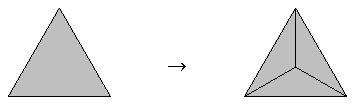
\includegraphics[width=0.40\paperwidth]{figures/Fig_012_PDF046_Book034.pdf}
  \caption{将三角形细分为三个小三角形（原书 p.34）}
  \label{fig:triangle-subdivision}
\end{figure}
证明新的单纯上链复形与原来的上链复形拟同构。
\end{exercise}

\begin{exercise}\label{exer:product-circle}
设 $X=|S|$ 是由 $\Delta$-集 $S$ 给出的拓扑空间，$S^1$ 是圆周。为 $X\times S^1$ 构造一个 $\Delta$-集，并利用它证明
\[
  H^k(X\times S^1,k)\cong H^{k-1}(X,k)\oplus H^k(X,k).
\]
\end{exercise}

\begin{exercise}\label{exer:surface-cohomology}
利用适当的 $\Delta$-集计算亏格为 $g$ 的紧致可定向曲面的上同调环。
\end{exercise}

\begin{exercise}\label{exer:torus-de-rham}
令 $T=\mathbb R^2/\mathbb Z^2$ 为环面，并考察 $\Omega^\bullet(T)$。作为 $C^\infty(T)$-模，它由 $1,dX,dY,dX\wedge dY$ 生成，其中 $X,Y$ 是 $\mathbb R^2$ 上的标准坐标。证明这些元素也构成德拉姆上同调环的一组基。将环面划分为两个三角形，并利用这一划分描述单纯上同调与德拉姆上同调之间的同构。
\end{exercise}

\begin{exercise}\label{exer:surface-group-ext}
考虑环
\[
  R=\frac{\mathbb C\langle X_1,Y_1,\ldots,X_g,Y_g\rangle}
  {\left\langle\sum_i(X_iY_i-Y_iX_i)\right\rangle},
\qquad
  S=R/\langle X_1,Y_1,\ldots,X_g,Y_g\rangle.
\]
计算 $S$ 的 Ext 环。
\end{exercise}

\begin{exercise}\label{exer:truncated-polynomial-ext}
令 $R=\mathbb C[\varepsilon]/(\varepsilon^3)$，$S=R/\langle\varepsilon\rangle$。计算 $S$ 的 Ext 环，并证明在这个环中可以定义一个非零的三元 Massey 积。
\end{exercise}

\begin{exercise}\label{exer:quiver-like-ext}
令
\[
  R=\frac{\mathbb C\langle e,u\rangle}
  {\langle e^2-e,\ eu-u,\ ue\rangle},
\qquad S=R/\langle u\rangle.
\]
证明 $S$ 的 Ext 环同构于 $R$ 本身。
\end{exercise}

\begin{exercise}\label{exer:finite-group-ext}
设 $G$ 是有限群，$V,W$ 是两个 $\mathbb CG$-模。证明当 $i>0$ 时
\[
  \operatorname{Ext}_{\mathbb CG}^i(V,W)=0.
\]
\end{exercise}

\chapterreview{%
\textbf{全章地位。}本章把复形确立为全书的基本工作单位，并把拓扑与代数两条上同调路线并置：一条由 $\Delta$-集通向杯积上同调环，一条由自由分解通向 Ext 环。这是为第 3 章的 $A_\infty$ 结构预备两个“信息不够用”的范例——上同调环丢掉 Massey 积，Ext 环只看得到关系的二次部分。

\textbf{知识脉络。}§2.1 给出上链复形、态射、拟同构与同伦，再用向量空间的分裂 $C^i=H^i\oplus I^i\oplus R^i$ 把拟同构的判定化归为对 $f^{HH}$ 的判定，并得到 $HK^0(k)\simeq\mathrm{grVECT}(k)$。§2.2 用 $\Delta$-集把“粘合空间”翻译成函子，以 $C_\Delta^\bullet(S,k)=\mathrm{Sets}(S[i],k)$ 与杯积建立上同调环，再由奇异上同调与德拉姆定理说明它只依赖 $|S|$。§2.3 把同一句式移植到代数：自由分解、比较定理、Ext 群、扩张的分类、Ext 环与 Koszul 分解。两节末尾各有一个缺口：Massey 积落在环结构之外，乘法又只能恢复二次关系；二者正好汇合，第 3 章由此展开。

\textbf{核心结论。}（1）复形分解为 $C^\bullet\cong C_m^\bullet\oplus C_c^\bullet$，其中 $C_m=H$ 极小、$C_c=I\oplus R$ 可缩，$d$ 在 $R^i\to I^{i+1}$ 上可逆；于是 $f$ 是拟同构当且仅当 $f^{HH}$ 是同构，$f$ 零同伦当且仅当 $f^{HH}=0$。（2）杯积使单纯上同调成为分次环，环面给出 $\Lambda_2=k\langle\xi,\eta\rangle/\langle\xi^2,\eta^2,\xi\eta+\eta\xi\rangle$；若 $|S|\cong X$，则 $HC_\Delta^\bullet(S,k)\cong H^\bullet(X,k)$ 为分次环同构，且 $\varphi\colon\Omega^\bullet(M)\to C_\Delta^\bullet(S,\mathbb R)$ 是拟同构。（3）比较定理保证自由分解间的提升存在且同伦唯一，故 $\operatorname{Ext}_A^i(M,N)$ 与分解的选取无关；$\operatorname{Ext}_A^1$ 按等价分类扩张；对 $A=k[X_1,\ldots,X_n]$ 与 $S=A/(X_1,\ldots,X_n)$，Koszul 分解给出 $\operatorname{Ext}_A^\bullet(S,S)\cong\Lambda_n$。（4）一般地 $\xi_i\xi_j=\sum_u\lambda^u_{ij}\rho_u$ 当且仅当关系 $r_u$ 的二次项为 $\sum_{ij}\lambda^u_{ij}X_jX_i$。

\textbf{辨析与提醒。}其一，“系数在域上”不能省：$\mathbb Z\xrightarrow{2}\mathbb Z$ 说明 $\mathbb Z$-模复形没有 $H\oplus I\oplus R$ 分裂，分解定理与引理\ref{lem:complex-map-criterion} 同时失效，这正是练习 2.1 的要点。其二，两种“上同调相同”并不等同：$|S_1|\cong|S_2|$ 只保证链层面有拟同构，而它一般不是环同构，故拓扑不变性须另证；Massey 积更须在链层面选取 $s,t$。其三，$\langle[u],[v],[w]\rangle$ 是集合而非单个类，符号随 $s,t$ 而变，只有退化为单元素时才“良定义”；第 3 章的 $\mu_3$ 只定到同伦，根源在此。其四，Ext 按上链复形定义，分解写在负次数（$P^0\leftarrow P^{-1}\leftarrow\cdots$），勿与同调次数混同。

\textbf{评注。}本章示范了“同一形式、两种实现”：$\Delta$-集上同调与 Ext 环最终在 $\Lambda_2$ 处重合（§2.3 末注），这就是镜像对称的基本观察。作者刻意只做域系数、只做自由分解，把一般阿贝尔范畴、谱序列与导出函子推给文献；代价是结论偏“玩具”，好处是每个证明都能写成矩阵，读者能亲手看到 $H\oplus I\oplus R$ 与 $h^2=0$、$dhd=d$、$hdh=h$ 这组收缩数据——第 3 章的树形公式正是把它们抽象成沿 $h$ 搬运结构的机器。读本章宜自问：哪些结论真正用到“域”，哪些只用到“复形”？上同调环丢掉的究竟是什么？若只记一个结论，应记住 $f^{HH}$ 这组矩阵分量：它把“拟同构”化为线性代数里的“可逆”。
}

% 第 3 章：高阶乘积
\chapter{高阶乘积}\label{ch:higher-products}
上一章中，我们看到，在上同调环上定义高阶乘积很有意义，因为取上同调的过程会丢失一些信息。本章将介绍由 Stasheff 最初发展的 $A_\infty$ 形式体系\bookcite{229}，它以协调一致的方式处理这些高阶乘积。随后，我们把这套形式体系与第一章的范畴论和表示论结合起来。最后还会考察这些思想的一些有用推广。

更多细节和背景材料可参见 Keller 的综述文章\bookcite{133}、\bookcite{135}，Seidel 著作的第一部分\bookcite{218}，以及 Kontsevich 与 Soibelman 的专著\bookcite{150}。

\section{动机与定义}\label{sec:ainfty-motivation}
\takeaway{微分、乘法与 Leibniz 律都是“两个运算复合后相消”的实例，可用根树统一图示；$A_\infty$ 代数把这三条恒等式推广为 $b_i\colon A[1]^{\otimes i}\to A[1]$ 上的一族 Stasheff 恒等式，$A_\infty$ 态射容许不同阶乘积混合；Koszul 符号是使 $\mu$ 与 $m$ 两种约定等价的枢纽。}
\subsection{推广结合律}\label{subsec:generalizing-associativity}
先考察此前遇到过的三种代数对象。上链复形是一个分次向量空间 $V$，带有一个次数为 $1$ 的一元运算 $\delta$，满足微分律 $\delta^2=0$。分次代数 $R$ 是一个分次向量空间，带有一个次数为 $0$ 的二元运算“$\cdot$”，满足结合律。第三种对象是 dg-代数，它同时具有这两种运算。每种运算各自满足相应恒等式，二者还须满足一条额外规律：分次 Leibniz 律。为了避免陷入符号细节，我们暂时假设工作域 $k$ 的特征为 $2$，并给出这三种看似不同的规律的一种统一解释。
% [Tutor Note: 假设 $\mathrm{char}\,k=2$ 时 $+1=-1$，所以下面三条恒等式里的所有符号都消失了；在特征 $0$ 的域上，须改用带 Koszul 符号的 $b_k$（见 §3.1.4），三条恒等式才严格成立。切勿把特征 $2$ 下的“统一解释”直接搬到特征 $0$。]

将恒等映射记作 $1$，令
\[
  \mu_1\colon V\to V,\quad v\longmapsto\delta v,
\qquad
  \mu_2\colon V^{\otimes2}\to V,\quad
  v\otimes w\longmapsto v\cdot w.
\]
于是三条规律可以写成
\begin{align*}
  [\mathrm{DIF}]&\quad \mu_1\circ\mu_1=0,\\
  [\mathrm{LEI}]&\quad
  \mu_1\circ\mu_2+\mu_2\circ(\mu_1\otimes1)
  +\mu_2\circ(1\otimes\mu_1)=0,\\
  [\mathrm{ASS}]&\quad
  \mu_2\circ(\mu_2\otimes1)+\mu_2\circ(1\otimes\mu_2)=0.
\end{align*}
这三条规律都表示某个算子（一元、二元或三元）为零。该算子是所有可能的、由两个运算复合而成的一元、二元或三元运算之和；为了让各映射能够复合，还要在必要位置与恒等映射作张量积。

若用根树的节点表示各个乘积，就可以把每条恒等式图示为所有具有两个节点、并分别有 $k=1,2,3$ 个叶子的树之和（不把输出端算作叶子）：
\begin{figure}[H]\centering
  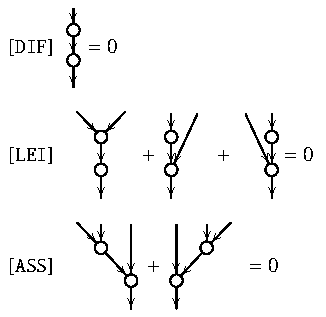
\includegraphics[width=0.32\paperwidth]{figures/Fig_013_PDF049_Book037.pdf}
  \caption{微分律、Leibniz 律与结合律的树形表示（原书 p.37）}
  \label{fig:basic-identity-trees}
\end{figure}
这种图示解释可以推广到所有 $k$。

\subsection{$A_\infty$ 代数}\label{subsec:ainfty-algebras}
\begin{definition}{$A_\infty$ 代数}{ainfty-algebra}
$A_\infty$ 代数\index{adaishu@$A_\infty$ 代数|hyperpage}是一个分次向量空间 $A^\bullet$，连同一列次数为 $1$ 的映射
\[
  b_i\colon A[1]^{\otimes i}\to A[1],\qquad i=1,2,\ldots,
\]
使得对所有 $n\geq1$ 都有恒等式
\[
  [M_n]\qquad
  \sum_{\substack{r+s+t=n\\r,t\geq0,\ s>0}}
  b_{r+t+1}\circ
  \bigl(1^{\otimes r}\otimes b_s\otimes1^{\otimes t}\bigr)=0.
\]
\end{definition}
上述公式可以图示为
\begin{figure}[H]\centering
  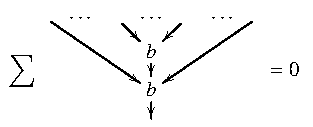
\includegraphics[width=0.37\paperwidth]{figures/Fig_014_PDF049_Book037.pdf}
  \caption{$A_\infty$ 代数恒等式的两节点树形表示（原书 p.37）}
  \label{fig:ainfty-algebra-trees}
\end{figure}
其中求和遍历所有具有 $n$ 个叶子、两个节点的根树。

\begin{note}
次数为 $1$ 的映射 $b_i\colon A[1]^{\otimes i}\to A[1]$，也可以看作次数为 $2-i$ 的映射
\[
  \mu_i\colon A^{\otimes i}\to A.
\]
从这个角度看，一元乘积的次数为 $1$，二元乘积的次数为 $0$，分别与微分和通常的乘积相同。这一次数约定也符合三元 Massey 积
\[
  \langle u,v,w\rangle
  =\bigl[u\,d^{-1}(vw)\pm d^{-1}(uv)\,w\bigr]
\]
的定义；三元 Massey 积的次数是 $-1=2-3$。此外，定理\ref{thm:ext-low-degrees}之后的讨论表明，高阶乘积应当记录关系的系数
\[
  \mu_k(\xi_1\otimes\cdots\otimes\xi_k)=\sum_i\lambda_i\rho_i,
\]
其中 $\xi_i\in\operatorname{Ext}_A^1(S,S)$，$\rho_i\in\operatorname{Ext}_A^2(S,S)$。因此，这里的次数同样为
\[
  \deg\rho_i-\deg\xi_1-\cdots-\deg\xi_k=2-k.
\]
\end{note}

\begin{note}
条件 $[M_1]$ 与 $[\mathrm{DIF}]$ 相同，因此 $(A[1],b_1)$ 总是一个上链复形。条件 $[M_2]$ 与 $[\mathrm{LEI}]$ 相同；若 $b_1=0$ 或 $b_3=0$，条件 $[M_3]$ 就化为 $[\mathrm{ASS}]$，因为其余各项都同时含有 $b_1$ 和 $b_3$。
\end{note}

\subsection{$A_\infty$ 态射}\label{subsec:ainfty-morphisms}
自然地，我们也希望定义 $A_\infty$ 代数之间的态射\index{ataishe@$A_\infty$ 态射|hyperpage}。直观上，人们可能会认为态射就是满足
\[
  b_k^B\circ f^{\otimes k}=f\circ b_k^A
\]
的映射 $f\colon A\to B$。遗憾的是，这个概念过于严格，因为它不允许不同乘积相互混合。它只能把 $A$ 的 $k$ 元乘积与 $B$ 的 $k$ 元乘积联系起来；但我们引入高阶乘积，正是为了在取同调时保留二元乘积的一些特征。因此，需要一种允许不同乘积相互混合的态射概念。

\begin{definition}{$A_\infty$ 态射}{ainfty-morphism}
$A_\infty$ 态射 $f_\bullet\colon A\to B$ 是一列次数为 $0$ 的映射
\[
  f_i\colon A[1]^{\otimes i}\to B[1],
\]
并满足以下公理：
\[
  [F_n]\qquad
  \sum_{\substack{r+s+t=n\\r,t\geq0,\ s>0}}
  f_{r+t+1}\circ
  \bigl(1^{\otimes r}\otimes b_s^A\otimes1^{\otimes t}\bigr)
  =
  \sum_{\substack{i_1+\cdots+i_k=n\\k>0,\ i_j>0}}
  b_k^B\circ(f_{i_1}\otimes\cdots\otimes f_{i_k}).
\]
两个 $A_\infty$ 态射 $f_\bullet\colon A\to B$ 和 $g_\bullet\colon B\to C$ 的复合定义为
\[
  (g\circ f)_n:=
  \sum_{\substack{i_1+\cdots+i_k=n\\k>0,\ i_j>0}}
  g_k\circ(f_{i_1}\otimes\cdots\otimes f_{i_k}).
\]
$[F_1]$ 表明，$f_1$ 是上链复形 $(A[1],b_1^A)$ 与 $(B[1],b_1^B)$ 之间的态射。若 $f_1$ 是上链复形同构\index{atonggou@$A_\infty$ 同构|hyperpage}，则称 $f_\bullet$ 为 $A_\infty$ 同构；若 $f_1$ 是拟同构\index{anitonggou@$A_\infty$ 拟同构|hyperpage}，则称 $f_\bullet$ 为 $A_\infty$ 拟同构。
\end{definition}

\begin{note}
$A_\infty$ 态射公理可以图示如下：
\begin{figure}[H]\centering
  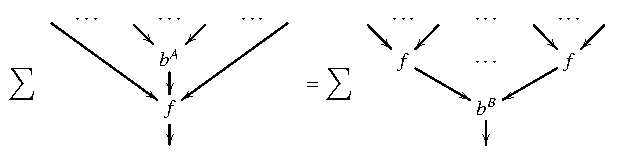
\includegraphics[width=0.77\paperwidth]{figures/Fig_015_PDF051_Book039.pdf}
  \caption{$A_\infty$ 态射公理的图示（原书 p.39）}
  \label{fig:ainfty-morphism-diagram}
\end{figure}
若所有高阶映射都为零（$f_{\geq2}=0$），就恢复了朴素的态射定义。这类态射称为严格 $A_\infty$ 态射。若 $g_\bullet\colon B^\bullet\to A^\bullet$ 是 $f_\bullet\colon A^\bullet\to B^\bullet$ 的（拟）逆，则要求它们的复合为严格态射，且 $g_1$ 是 $f_1$ 的（拟）逆。于是 $(f\circ g)_1$ 和 $(g\circ f)_1$ 分别（同伦于）恒等映射。
\end{note}

\begin{lemma}{$A_\infty$ 态射的逆}{ainfty-morphism-inverse}
设 $f_\bullet\colon A^\bullet\to B^\bullet$ 是一个 $A_\infty$ 态射。
\begin{enumerate}
  \item $f_\bullet$ 有逆，当且仅当它是 $A_\infty$ 同构；
  \item $f_\bullet$ 有拟逆，当且仅当它是 $A_\infty$ 拟同构。
\end{enumerate}
\end{lemma}
\begin{proof}[证明思路]
思路是逐步构造（拟）逆 $g_\bullet$。先构造 $g_1$：由于 $f_1$ 是（拟）同构，由引理\ref{lem:complex-map-criterion}可取其（拟）逆 $g_1$。更高阶的 $g_i$ 可由条件 $(g\circ f)_{>0}=0$ 归纳确定。例如，若 $g_1$ 是同构且 $(g\circ f)_2=0$，则
\[
  g_2(f_1\otimes f_1)+g_1f_2=0,
\]
因此
\[
  g_2=-g_1f_2(f_1^{-1}\otimes f_1^{-1})
      =-g_1f_2(g_1\otimes g_1).
\]
另见\bookcite[I 1.14]{218}。
\end{proof}

与复形态射一样，$A_\infty$ 态射的强大之处在于拟同构可以取拟逆。若只允许严格态射，这一点便不再成立。严格态射的拟逆一般不再严格，因为要使它满足公理 $[F_n]$，通常需要非零的高阶分量。

\subsection{处理符号}\label{subsec:sign-conventions}
若工作域的特征为 $0$，乘积 $b_2$ 并不给出通常意义下的乘积，因为结合律只在相差符号的意义下成立。因此，需要额外引入符号才能使各项协调一致。处理这一问题有多种方法；简要综述可参见\bookcite{202}。

起点是 Koszul 符号约定，它规定如何让算子作用于输入元。

\begin{definition}{Koszul 符号约定}{koszul-sign}
设 $\varphi\colon V^{\otimes k}\to V$、$\psi\colon V^{\otimes l}\to V$ 是两个分次线性算子。定义它们的张量积在 $V^{\otimes(k+l)}$ 上的左作用为
\[
  (\varphi\otimes\psi)
  (a_1\otimes\cdots\otimes a_k\otimes b_1\otimes\cdots\otimes b_l)
  =
  (-1)^{|\psi|(|a_1|+\cdots+|a_k|)}
  \varphi(a_1\otimes\cdots\otimes a_k)
  \otimes
  \psi(b_1\otimes\cdots\otimes b_l),
\]
其中 $|a|$ 简记元素 $a$ 的次数。
\end{definition}
换言之，Koszul 规则是：每当一个奇次数算子越过一个奇次数元素时，就要引入一个负号。这个经验法则也能给出算子从右侧作用时的公式：
\[
  (a_1\otimes\cdots\otimes a_k\otimes b_1\otimes\cdots\otimes b_l)
  (\varphi\otimes\psi)
  =
  (-1)^{|\varphi|(|b_1|+\cdots+|b_l|)}
  \varphi(a_1\otimes\cdots\otimes a_k)
  \otimes\psi(b_1\otimes\cdots\otimes b_l).
\]
从这里开始，有两种主要的符号约定：一种主要用于辛几何，另一种主要用于表示论。

\subsubsection*{辛几何约定}
Seidel 的著作\bookcite{218}与大多数关于 Fukaya 范畴的论文都采用这种约定。令移位后的乘积 $b_\bullet$ 和 $A_\infty$ 态射 $f_\bullet$ 从右侧作用，并定义
\[
  \mu_k(a_1,\ldots,a_k)
  :=\bigl((a_1[1]\otimes\cdots\otimes a_k[1])b_k\bigr)[-1],
\]
\[
  \varphi_k(a_1,\ldots,a_k)
  :=\bigl((a_1[1]\otimes\cdots\otimes a_k[1])f_k\bigr)[-1],
\]
其中 $a[1]$ 表示把 $a\in A$ 看作 $A[1]$ 中的元素；在 $A[1]$ 中它的次数降低 $1$。由此得到以下版本的 $A_\infty$ 公理：
\[
  [\mathrm{SM}_n]\qquad
  \sum_{r+s+t=n}(-1)^\dagger
  \mu_{r+t+1}(a_1,\ldots,a_r,\mu_s(a_{r+1},\ldots,a_{r+s}),
       a_{r+s+1},\ldots,a_{r+s+t})=0,
\]
其中
\[
  \dagger=(|a_{r+s+1}|-1)+\cdots+(|a_{r+s+t}|-1).
\]
指数中出现 $|a_{r+s+1}|-1$，是因为输入元素的次数已经移位。
% [Tutor Note: 这里 $|\cdot|$ 是元素在 $A$ 中的次数，不是移位后在 $A[1]$ 中的次数，所以每越过一个输入就贡献 $(|a|-1)$；若误把输入当成 $A[1]$ 的元素（次数 $|a|-1$）再算，会多出符号。另一处常见混淆是 $\mu$ 与 $m$ 两套约定：$m_k=\sigma^{-1}\circ b_k\circ\sigma^{\otimes k}$ 不带额外符号，而 $\mu$ 由右作用 $\bigl((a_1[1]\otimes\cdots\otimes a_k[1])b_k\bigr)[-1]$ 定出，两者只差整体符号约定，切勿混用。]

若 $A_\infty$ 代数满足 $\mu_{\geq3}=0$，则规则 $[\mathrm{SM}_2]$ 与 $[\mathrm{SM}_3]$ 分别化为
\[
  \mu_1(\mu_2(a,b))
  +(-1)^{|b|-1}\mu_2(\mu_1(a),b)
  +\mu_2(a,\mu_1(b))=0,
\]
\[
  (-1)^{|c|-1}\mu_2(\mu_2(a,b),c)
  +\mu_2(a,\mu_2(b,c))=0.
\]
遗憾的是，这两式都不是通常的 Leibniz 律或结合律。可以通过另外定义
\[
  da:=(-1)^{|a|}\mu_1(a),
  \qquad
  a\cdot b:=(-1)^{|b|}\mu_2(a,b)
\]
来解决。于是有
\begin{align*}
  &(-1)^{|a|+|b|+|b|}d(a\cdot b)
  +(-1)^{|b|-1+|a|+|b|}da\cdot b
  +(-1)^{|b|+|b|+1}a\cdot db=0,\\
  &(-1)^{|a|}\bigl(d(a\cdot b)-da\cdot b-(-1)^{|a|}a\cdot db\bigr)=0,\\
  &(-1)^{|c|-1+|b|+|c|}(a\cdot b)\cdot c
  +(-1)^{|b|+|c|+|c|}a\cdot(b\cdot c)=0,\\
  &(-1)^{|b|-1}\bigl((a\cdot b)\cdot c-a\cdot(b\cdot c)\bigr)=0.
\end{align*}
对 $A_\infty$ 态射，相应的符号规则为
\[
  [\mathrm{SF}_n]\qquad
  \sum_{\substack{r+s+t=n\\r,t\geq0,\ s>0}}(-1)^\dagger
  \varphi_{r+t+1}\circ
  (1^{\otimes r}\otimes\mu_s^A\otimes1^{\otimes t})
  =
  \sum_{\substack{i_1+\cdots+i_k=n\\k>0,\ i_j>0}}
  \mu_k^B\circ(\varphi_{i_1}\otimes\cdots\otimes\varphi_{i_k}).
\]
注意，$\varphi$ 前面没有额外符号，因为它们的移位版本次数为 $0$。

\subsubsection*{表示论约定}
Keller 的综述文章\bookcite{133}、\bookcite{135}与许多高阶代数论文采用这种约定。先定义次数为 $-1$ 的映射
\[
  \sigma\colon A\to A[1],\qquad x\longmapsto(-1)^{|x|}x[1].
\]
令移位后的乘积 $b_\bullet$ 和 $A_\infty$ 态射 $f_\bullet$ 从左侧作用，并定义未移位乘积
\[
  m_k(a_1,\ldots,a_k)
  :=\sigma^{-1}\circ b_k\circ\sigma^{\otimes k}
       (a_1\otimes\cdots\otimes a_k).
\]
态射分量也按相同方式解除移位：若把移位后的分量记为 $f_k^{\mathrm{sh}}$，则令
\[
  f_k(a_1,\ldots,a_k)
  :=\sigma_B^{-1}\circ f_k^{\mathrm{sh}}\circ\sigma_A^{\otimes k}
       (a_1\otimes\cdots\otimes a_k).
\]
这样得到的 $A_\infty$ 公理为
\[
  [\mathrm{RM}_n]\qquad
  \sum_{r+s+t=n}(-1)^\epsilon
  m_{r+t+1}(a_1,\ldots,a_r,m_s(a_{r+1},\ldots,a_{r+s}),
      a_{r+s+1},\ldots,a_{r+s+t})=0,
\]
其中
\[
  \epsilon=r+st+s(|a_1|+\cdots+|a_r|).
\]
注意，在这种约定下，Leibniz 律和结合律会自动出现：
\begin{align*}
  &(-1)^{0+2\cdot0}m_1(m_2(a,b))
  +(-1)^{0+1\cdot1}m_2(m_1(a),b)
  +(-1)^{1+1\cdot0+|a|}m_2(a,m_1(b))=0,\\
  &(-1)^{0+2\cdot1}m_2(m_2(a,b),c)
  +(-1)^{1+2\cdot0+2|a|}m_2(a,m_2(b,c))=0.
\end{align*}

\begin{note}
我们始终用字母 $b$ 记移位后的映射，用拉丁字母 $m$ 记表示论约定，用希腊字母 $\mu$ 记辛几何约定。由于研究 Fukaya 范畴时后一种约定十分重要，下面大多采用 $\mu$-乘积，并以带有相应符号的 $\mu$-乘积表述定义。这些符号来自只含加号的 $b$-乘积定义。
\end{note}

\subsection{例子}\label{subsec:ainfty-examples}
\begin{example}[普通代数]\label{ex:ordinary-algebra-ainfty}
任意普通代数 $(R,\cdot)$ 都可以看成集中在次数 $0$ 的 $A_\infty$ 代数 $R^\bullet$，其中 $\mu_2(x,y)=x\cdot y$，且 $\mu_i=0$（$i\neq2$）。
\end{example}

\begin{example}[微分分次代数]\label{ex:dg-algebra-ainfty}
若 $(A,d,\cdot)$ 是 dg-代数，我们将其视为具有如下 $\mu$-乘积的 $A_\infty$ 代数：
\[
  da:=(-1)^{|a|}\mu_1(a),
  \qquad
  a\cdot b:=(-1)^{|b|}\mu_2(a,b).
\]
\end{example}

\begin{example}[dg-代数拟同构不必反向存在]\label{ex:dg-quasiisomorphism-ainfty}
考虑普通代数 $R=k[X]/(X^2)$ 和 dg-代数 $A=k[X,Y]/(Y^2)$，其中 $|X|=0$、$|Y|=-1$，且 $dY=X^2$。由于 $R^\bullet$ 是 $A^\bullet$ 的同调，存在 dg-代数拟同构 $\pi\colon A^\bullet\to R^\bullet$；它对应于一个严格的 $A_\infty$ 拟同构。

反方向不存在 dg-代数拟同构，因为 $X^2$ 在 $R$ 中为零，而 $A$ 的零次部分没有零因子。不过，我们可以构造一个 $A_\infty$ 拟同构 $\varphi_\bullet\colon R^\bullet\to A^\bullet$，令
\[
  \varphi_1(a+bX)=a+bX,\qquad
  \varphi_2(1,X)=\varphi_2(X,1)=0,\qquad
  \varphi_2(X,X)=Y.
\]
由次数考虑，所有更高阶的 $\varphi_i$ 都必须为零。对于 $(X,X)$，$A_\infty$ 规则 $[\mathrm{SF}_2]$ 变成
\[
  \varphi_1\mu_2^R(X,X)
  =\mu_2^A(\varphi_1(X),\varphi_1(X))
   +\mu_1^A(\varphi_2(X,X)),
\]
也就是
\[
  0=X^2+(-1)^{|Y|}dY=X^2-X^2.
\]
\end{example}

\begin{example}[形式幂级数与 $A_\infty$ 结构]\label{ex:ainfty-formal-series}
设 $r\in k[[X]]$ 是常数项为零的形式幂级数：
\[
  r=r_1X+r_2X^2+r_3X^3+\cdots.
\]
令 $A=k\xi\oplus k\rho$，其中 $|\xi|=1$、$|\rho|=2$。定义如下 $A_\infty$ 结构：
\[
  \mu_k^r(\xi,\ldots,\xi)=r_k\rho,
\]
而所有含有 $\rho$ 的乘积都规定为零。容易验证这些乘积满足 $A_\infty$ 公理。

再取另一个形式幂级数
\[
  f=f_1X+f_2X^2+\cdots\in k[[X]].
\]
它定义环同态
\[
  \iota_f\colon k[[X]]\to k[[X]],\qquad
  u(X)\longmapsto u(f(X)).
\]
令 $s=\iota_f(r)$。定义 $A_\infty$ 映射 $\varphi_k^f\colon A^{\otimes k}\to A$：
\[
  \varphi_k^f(\xi,\ldots,\xi)=f_k\xi.
\]
所有含有 $\rho$ 的表达式都映为零，只有 $\varphi_1^f(\rho)=\rho$ 例外。于是得到从 $(A,\mu^s)$ 到 $(A,\mu^r)$ 的 $A_\infty$ 态射。其关键恒等式为
\begin{align*}
  &\mu_k^r\bigl(\varphi_{i_1}^f(\xi,\ldots,\xi),\ldots,
                       \varphi_{i_k}^f(\xi,\ldots,\xi)\bigr)\\
  &\quad=\sum_{i_1+\cdots+i_k=n}
       \mu_k^r(f_{i_1}\xi,\ldots,f_{i_k}\xi)
   =\sum_{i_1+\cdots+i_k=n}f_{i_1}\cdots f_{i_k}r_k\rho\\
  &\quad=\varphi_1^f\mu_n^s(\xi,\ldots,\xi)
   =\sum_{i+j+k=n}
     \varphi^f(\ldots,\mu_j^s(\xi,\ldots,\xi),\ldots).
\end{align*}
两个这样的 $A_\infty$ 态射的复合，对应于 $k[[X]]$ 上两个环同态的复合：
\[
  \varphi_\bullet^f\circ\varphi_\bullet^g=\varphi_\bullet^h,
  \qquad \iota_f\circ\iota_g=\iota_h.
\]
最后，若 $f_1\neq0$，则 $\iota_f$ 可逆，因此 $\varphi_\bullet^f$ 是 $A_\infty$ 同构。从某种意义上说，$A$ 上的 $A_\infty$ 结构与 $k[[X]]$ 中的元素互为对偶。
\end{example}

\begin{note}
还可以在前一个例子中加入一个次数为 $0$ 的单位元：
\[
  E^\bullet=k1\oplus k\xi\oplus k\rho.
\]
对乘积增加如下规则：对任意齐次元 $u\in E^\bullet$，
\[
  \mu_2^r(u,1)=(-1)^{|u|}\mu_2^r(1,u)=u;
\]
而所有其他含有 $1$ 的乘积均规定为零。
\end{note}

\section{极小模型}\label{sec:minimal-models}
\takeaway{用复形分裂定理把 $A_\infty$ 代数拆成可缩部分与极小部分的直和；极小模型由对树求和定义，故在 $A_\infty$ 同构意义下唯一；同调扰动引理把这套树形公式推广到任意拟同构，是 dg-模型与极小模型互转的工具。}
\subsection{结构定理}\label{subsec:ainfty-structure-theorem}
与向量空间复形类似，$A_\infty$ 代数也有一个结构定理，它允许我们把每个 $A_\infty$ 代数分解为两部分的直和。

\begin{definition}{极小与可缩的 $A_\infty$ 结构}{minimal-contractible-ainfty}
$A_\infty$ 结构 $(A,b)$ 称为
\begin{itemize}
  \item 极小的，若 $b_1=0$；
  \item 可缩的，若 $b_{>1}=0$ 且 $H(A)=0$。
\end{itemize}
\end{definition}

\begin{theorem}{Kadeishvili 极小模型定理}{kadeishvili-minimal-model}
每个 $A_\infty$ 代数都 $A_\infty$ 同构于一个可缩 $A_\infty$ 代数\index{kesuoadaishu@可缩 $A_\infty$ 代数|hyperpage}与一个极小 $A_\infty$ 代数\index{jixiaoadaishu@极小 $A_\infty$ 代数|hyperpage}的直和\bookcite{131}。
\end{theorem}
\begin{proof}[证明思路]
这里概述 Kontsevich 与 Soibelman 的证明\bookcite{147}，因为它有很好的图示解释。Merkulov 和 Markl 的其他较详细论述见\bookcite{174}、\bookcite{170}。

设 $A$ 是一个 $A_\infty$ 代数。对 $A$ 上的微分 $-b_1$，按照引理\ref{lem:complex-map-criterion}选取分解
\[
  A^\bullet=I^\bullet\oplus H^\bullet\oplus R^\bullet.
\]
这给出一个映射 $h$ 与投影
\[
  \pi=1+b_1h+hb_1,
\]
其像为 $H^\bullet$。
\begin{figure}[H]\centering
  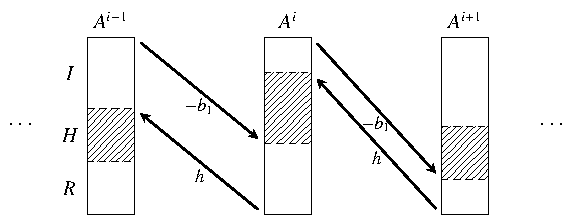
\includegraphics[width=0.46\paperwidth]{figures/Fig_016_PDF055_Book043.pdf}
  \caption{上链复形 $(A,b_1)$ 的极小与可缩部分（原书 p.43）}
  \label{fig:ainfty-minimal-splitting}
\end{figure}
上链复形 $(A,b_1)$ 分解为 $A_{\mathrm{contr}}\oplus A_{\min}$，其中
\[
  A_{\mathrm{contr}}=I^\bullet\oplus R^\bullet=\ker\pi,
  \qquad
  A_{\min}=H^\bullet=\operatorname{im}\pi.
\]
\end{proof}

新结构 $\bar b$ 应当与上述分解相容，并且要构造 $(A,b)$ 与 $(A,\bar b)$ 之间的 $A_\infty$ 同构 $f_\bullet$。我们保留一元乘积不变，即 $\bar b_1=b_1$。要计算更高阶的 $\bar b_k$，考察具有 $k$ 个叶子的树。对每一棵这样的树 $T$，都可以构造一个乘积 $b_T$：每个叶子表示映射 $\pi$，每个节点表示某个映射 $b_i$，每条内部边表示映射 $h$，而树干表示 $\pi$。

\begin{figure}[H]\centering
  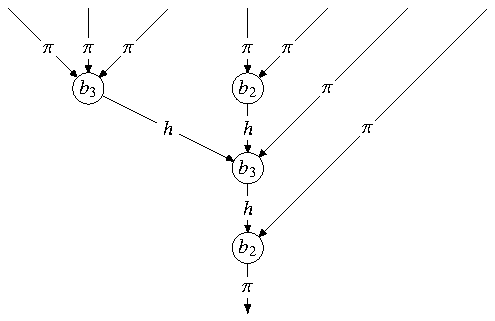
\includegraphics[width=0.43\paperwidth]{figures/Fig_017_PDF056_Book044.pdf}
  \caption{由树构造高阶乘积的示意图（原书 p.44）}
  \label{fig:tree-higher-products}
\end{figure}
上图对应的乘积为
\[
  b_T=\pi b_2\bigl(hb_3(hb_3\pi^{\otimes3}\otimes hb_2\pi^{\otimes2}\otimes\pi)\otimes\pi\bigr).
\]
定义新乘积为所有这些 $b_T$ 之和：
\[
  \bar b_k:=\sum_T b_T.
\]
% [Tutor Note: 书中只说“每个节点表示某个映射 $b_i$”，未限定 $i\geq2$。若允许 $b_1$ 作节点标记，$k$ 个叶子的树可以带任意长的 $b_1$ 单链，$\bar b_k$ 的定义就不再是有限和（形式的 $\partial_h$ 也需要幂级数收敛性才能逐项求导）。标准约定只取 $i\geq2$：每个内节点至少 $2$ 个儿子，故含 $k$ 个叶子的树至多 $k-1$ 个内节点，求和确为有限和。]
由于 $b_T$ 中都含有 $\pi$，新高阶乘积 $\bar b_\bullet$ 的像落在 $A_{\min}$ 中；只要某个输入属于 $A_{\mathrm{contr}}$，它就为零。另一方面，$\bar b_1$ 的像落在 $A_{\mathrm{contr}}$ 中，并且在 $A_{\min}$ 上为零。因此
\[
  (A,\bar b)=(A_{\mathrm{contr}},\bar b_1)\oplus(A_{\min},\bar b_{>1}).
\]

为证明 $\bar b$ 满足 $A_\infty$ 关系，注意算子 $\bar b_k$ 依赖于 $h$，可以对其求偏导：
\[
  \partial_h\bar b_k[u]
  :=\lim_{\varepsilon\to0}
  \frac{\bar b_k^{h+\varepsilon u}-\bar b_k^h}{\varepsilon}.
\]
这个导数等于把每棵树中的一条 $h$ 替换成 $u$ 后所得各项之和。若令 $u=\pi^2$，并沿这两个 $\pi$ 之间的边把树切开，就得到两棵较小的树。因此
\[
  \partial_h\bar b_k[\pi^2]
  =\sum_T\sum_{\substack{\text{树 }T\text{ 中}\\\text{的一条边 }h}}b_T
  =\sum_{T_1,T_2}
    b_{T_1}(\cdots\otimes b_{T_2}\otimes\cdots).
\]
表达式 $\partial_h\bar b_k[\pi^2]$ 实际上组合了所有成对出现的高阶乘积 $\bar b_{\geq2}$。这几乎就是 $\bar b$ 的 $A_\infty$ 关系，除了含有 $\bar b_1$ 的项。幸运的是，所有一个因子为 $\bar b_1$、另一个因子为 $\bar b_{\geq2}$ 的项都为零，因为 $b_1\pi=\pi b_1=0$。因此，$\bar b$ 的 $A_\infty$ 关系 $[M_k]$ 可以写成
\[
  \partial_h\bar b_k[\pi^2]=0.
\]
代入
\[
  \pi^2=\pi=1+b_1h+hb_1
\]
后，有
\[
  \partial_h\bar b_k[\pi^2]
  =\partial_h\bar b_k[1]
   +\partial_h\bar b_k[b_1h]
   +\partial_h\bar b_k[hb_1].
\]
最后两项是对所有树和边求和，其中 $b_1$ 被插在该边之前或之后。和中的每一项都含有 $b_l(\cdots b_1\cdots)$ 或 $b_1b_l$，其中 $l\geq2$。利用 $b$ 的 $A_\infty$ 关系，可将这些项改写成所有 $b_r(\cdots b_s\cdots)$ 的负和，其中 $r,s\geq2$。这样的乘积将 $b_r$ 与 $b_s$ 直接相连，中间没有 $h$，所以得到的都是把一条 $h$ 替换成 $1$ 的树。因此
\[
  \partial_h\bar b_k[b_1h]+\partial_h\bar b_k[hb_1]
  =-\partial_h\bar b_k[1],
\]
从而 $\partial_h\bar b_k[\pi^2]=0$，故 $\bar b$ 满足 $A_\infty$ 公理。

证明 $(A,b)$ 与 $(A,\bar b)$ 之间存在满足 $f_1=1$ 的 $A_\infty$ 同构 $f_\bullet$，只需进行类似计算。$f_i$ 的公式与 $\bar b_i$ 相同，只是树根处用映射 $h$ 代替 $\pi$。

\begin{note}
注意，对序列 $a_1\otimes\cdots\otimes a_n$ 使用 $\bar b$ 的公式时，不会出现来自 Koszul 规则的额外符号，因为所有涉及的映射（$\pi$ 和 $h\circ b$）次数都是偶数。因此，该公式对 $\mu$-乘积也成立，无须额外加入符号。

由于 $(A,\bar b)$ 是直和，嵌入 $A_{\min}\hookrightarrow A$ 和投影 $A\to A_{\min}$ 都是严格态射。

将嵌入与 $f_\bullet$ 的逆 $f_\bullet^{-1}\colon(A,\bar b)\to(A,b)$ 复合，并将投影与 $f_\bullet\colon(A,b)\to(A,\bar b)$ 复合，就得到映射
\[
  i_\bullet\colon A_{\min}\to(A,b),\qquad
  p_\bullet\colon(A,b)\to A_{\min}.
\]
若 $g_\bullet\colon A^\bullet\to B^\bullet$ 是 $A_\infty$ 拟同构，则
\[
  p_\bullet^B\circ g_\bullet\circ i_\bullet^A
\]
是两个极小模型之间的 $A_\infty$ 同构。反过来，若 $g_\bullet\colon A_{\min}^\bullet\to B_{\min}^\bullet$ 是 $A^\bullet,B^\bullet$ 的极小模型之间的 $A_\infty$ 同构，则
\[
  i_\bullet^B\circ g_\bullet\circ p_\bullet^A
\]
是 $A^\bullet$ 与 $B^\bullet$ 之间的 $A_\infty$ 拟同构。
\end{note}

\begin{corollary}{极小模型刻画拟同构}{minimal-models-characterize-quasi-isomorphism}
两个 $A_\infty$ 代数 $A_\infty$ 拟同构，当且仅当它们的极小模型 $A_\infty$ 同构。
\end{corollary}

自然的想法是构造 $A_\infty$ 代数的极小模型，并只研究极小模型，因为它们在 $A_\infty$ 同构意义下唯一确定。然而，实际算出极小模型的所有乘积出了名地困难；给定两个极小模型，要检验它们是否 $A_\infty$ 同构也很困难。

在另一端，也可以构造 dg-模型。它们是没有高阶乘积的 $A_\infty$ 代数，即 $b_{\geq3}=0$。dg-模型的优点是代数结构较容易处理，缺点则是含有许多在取同调时会被删去的额外元素。

具体应用不同，dg-模型或极小模型可能各有优势。$A_\infty$ 形式体系提供了一个框架，使我们能够相对容易地在不同模型之间转换。这可以借助同调扰动引理\index{tongdiaoraodongyinli@同调扰动引理|hyperpage}完成；它是极小模型定理的推广。

\begin{lemma}{同调扰动引理}{homological-perturbation-lemma}
设 $\varphi\colon A\to B$ 和 $\varphi^\dagger\colon B\to A$ 是两个复形 $(A,\mu_1^A)$、$(B,\mu_1^B)$ 之间互为拟逆的映射，并取映射 $h\colon B\to B$，满足
\[
  \varphi\varphi^\dagger=1_B+h\mu_1^B+\mu_1^Bh.
\]
\begin{figure}[H]\centering
  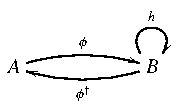
\includegraphics[width=0.35\paperwidth]{figures/Fig_018_PDF058_Book046.pdf}
  \caption{同调扰动引理中的链映射与同伦（原书 p.46）}
  \label{fig:homological-perturbation}
\end{figure}
若 $\mu_B^\bullet$ 是 $B$ 上延拓 $\mu_1^B$ 的一个 $A_\infty$ 结构，则可以把 $\mu_1^A$ 延拓为 $A_\infty$ 结构 $\mu_A^\bullet$，并构造 $A_\infty$ 拟同构 $\varphi_\bullet\colon A\to B$，使得 $\varphi_1=\varphi$。
\end{lemma}
\begin{proof}[证明思路]
思路相同：$\mu_n^A$ 是对所有树求和得到的，树节点标记为 $\mu_B$，叶子处是 $\varphi$，树根处是 $\varphi^\dagger$，内部边上是 $h$；构造 $\varphi_\bullet$ 时也用相同方法，只把树根处的映射换成 $h$。递归地，可以写为
\begin{align*}
  \mu_n^A(a_1,\ldots,a_n)
  &=
  \sum_r\ \sum_{\substack{i_1+\cdots+i_r=n\\i_j>0}}
  \varphi^\dagger\mu_r^B\bigl(
  \varphi_{i_1}(a_1,\ldots,a_{i_1}),\ldots,
  \varphi_{i_r}(a_{n-i_r+1},\ldots,a_n)\bigr),\\
  \varphi_n(a_1,\ldots,a_n)
  &=
  \sum_r\ \sum_{\substack{i_1+\cdots+i_r=n\\i_j>0}}
  h\mu_r^B\bigl(
  \varphi_{i_1}(a_1,\ldots,a_{i_1}),\ldots,
  \varphi_{i_r}(a_{n-i_r+1},\ldots,a_n)\bigr).
\end{align*}
更多细节见\bookcite{170}。
% [Tutor Note: 这两式都略去了下标与求和限制。$\mu_n^A$ 的式子右端用 $b$ 的 $\mu_r^B$ 与输入端的 $\varphi$，此时 $\varphi$ 已由下式先构造好，故 $r=1,\ i_1=n$ 也可；但 $\varphi_n$ 的递推必须取 $r\geq2$（即每个 $\varphi_{i_j}$ 的下标 $i_j\leq n-1$），否则右端会出现 $\mu_1^B\varphi_n$ 自身造成循环。书中把两式写成同一形式，读者需自行补上这一限制。]
\end{proof}

\subsection{例子}\label{subsec:minimal-model-examples}
\begin{example}[多项式环的 Ext 代数极小模型]\label{ex:minimal-model-polynomial}
回到例\ref{ex:ext-polynomial-two-variables}中的多项式环 $R=k[X,Y]$ 与 $S=R/(X,Y)$。我们已经知道
\[
  \operatorname{Ext}_R^\bullet(S,S)
  =\frac{k\langle\xi,\eta\rangle}
  {\langle\xi^2,\eta^2,\xi\eta+\eta\xi\rangle}.
\]
这个计算是通过考察 $\operatorname{Hom}_R^\bullet(K^\bullet,K^\bullet)$ 的上同调得到的，其中
\[
  K^\bullet:=R\xrightarrow{\binom{X}{-Y}}R^2
  \xrightarrow{(X\ \ Y)}R.
\]

除了上同调分次外，还可以给 $K^\bullet$ 加上第二种分次：把 $R$ 看成 $X,Y$ 次数均为 $1$ 的分次环。就这个第二分次而言，$\iota,\xi,\eta,\rho$ 的次数都是 $0$，因为例\ref{ex:ext-polynomial-two-variables}中的计算表明，这些映射只含常数。微分 $b_1$ 的第二次数为 $1$，因为它关于 $X,Y$ 是线性的。如果选取与新分次相容的分解 $H\oplus I\oplus R$，则 $h$ 的次数为 $-1$。

构造高阶乘积时需要对所有树求和。树的每个节点都是普通乘积，故其第二次数为 $0$；每条内部边的第二次数为 $-1$，因为它表示 $h$。因此，所有高阶乘积的第二次数都为负数。由于 $\operatorname{Ext}_R^\bullet(S,S)$ 只含第二次数为 $0$ 的元素，可以得出所有高阶乘积均为零。
\end{example}

\begin{example}[非零三元乘积]\label{ex:nonzero-triple-product}
考察
\[
  A=\frac{k\langle X,Y\rangle}{\langle X^2Y\rangle},
\]
并令 $S=A/(X,Y)$ 为 $X,Y$ 均平凡作用的简单右模。该模的 Koszul 分解为
\[
  K^\bullet:=A\xrightarrow{\binom{XY}{0}}A^{\oplus2}
  \xrightarrow{(X\ \ Y)}A.
\]
其 Ext 代数为
\[
  \operatorname{Ext}_A^\bullet(S,S)
  =k\iota\oplus(k\xi\oplus k\eta)\oplus k\rho.
\]
我们可以将这四个生成元提升为复形态射：
\begin{figure}[H]\centering
  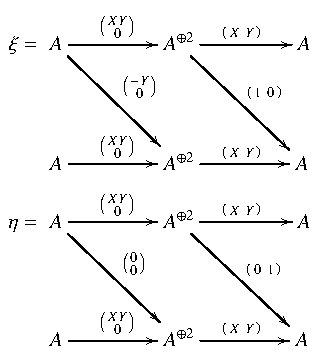
\includegraphics[width=0.48\paperwidth]{figures/Fig_019_PDF059_Book047.pdf}
  \caption{Ext 代数生成元 $\xi,\eta$ 的复形态射提升（原书 p.47）}
  \label{fig:nonzero-massey-generators}
\end{figure}
从这些表达式可知
\[
  \eta\cdot\xi=\eta\cdot\eta=\xi\cdot\eta=0,
\]
而 $\xi\cdot\xi$ 可由下图表示：
\begin{figure}[H]\centering
  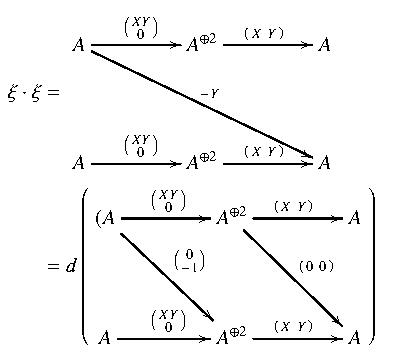
\includegraphics[width=0.46\paperwidth]{figures/Fig_020_PDF060_Book048.pdf}
  \caption{$\xi\cdot\xi$ 在 Hom 复形中为边界（原书 p.48）}
  \label{fig:xi-square-boundary}
\end{figure}
因此，尽管 $\xi\cdot\xi$ 在 $\operatorname{Hom}_A^\bullet(S,S)$ 中非零，它在上同调中为零：$\xi\cdot\xi=d\kappa$。由于 $\xi,\kappa$ 的次数均为 $1$，这一恒等式写成
\[
  -\mu_2(\xi,\xi)=-\mu_1(\kappa).
\]
在 $\operatorname{Hom}_A^\bullet(K^\bullet,K^\bullet)$ 中选取分解 $R\oplus H\oplus I$，其基包含 $\iota,\xi,\eta,\rho\in H$、$\xi\cdot\xi\in I$ 和 $\kappa\in R$。于是
\[
  h\mu_2(\xi,\xi)=-\kappa.
\]
计算 $\bar\mu_3$ 时，需要对下列两棵树求和：
\begin{figure}[H]\centering
  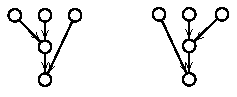
\includegraphics[width=0.29\paperwidth]{figures/Fig_021_PDF060_Book048.pdf}
  \caption{三元高阶乘积对应的两棵树（原书 p.48）}
  \label{fig:triple-product-trees}
\end{figure}
由此得到三元乘积
\begin{align*}
  \bar\mu_3(\eta,\xi,\xi)
  &=\pi\bigl(\mu_2(h\mu_2(\eta,\xi),\xi)
            +\mu_2(\eta,h\mu_2(\xi,\xi))\bigr)\\
  &=\pi(0-\mu_2(\eta,\kappa))
   =\pi(\eta\cdot\kappa)=-\rho,
\end{align*}
它非零。另一方面，
\begin{align*}
  \bar\mu_3(\xi,\xi,\eta)
  &=\pi\bigl(\mu_2(h\mu_2(\xi,\xi),\eta)
            +\mu_2(\xi,h\mu_2(\xi,\eta))\bigr)\\
  &=\pi(-\mu_2(\kappa,\xi)-0)
   =\pi(\kappa\cdot\xi)=0.
\end{align*}
这个例子可以推广为以下定理。
\end{example}

\begin{theorem}{Lu、Palmieri、Wu、Zhang 定理}{lu-palmieri-wu-zhang}
见\bookcite{168}。设
\[
  A=\frac{k\langle X_1,\ldots,X_n\rangle}
  {\langle r_1,\ldots,r_m\rangle}
\]
是一个极小表现，$S=A/\langle X_1,\ldots,X_n\rangle$ 是相应的简单模。$\operatorname{Ext}_A^\bullet(S,S)$ 的极小模型满足：
\begin{enumerate}
  \item $\operatorname{Ext}_A^1(S,S)=k\xi_1\oplus\cdots\oplus k\xi_n$；
  \item $\operatorname{Ext}_A^2(S,S)=k\rho_1\oplus\cdots\oplus k\rho_m$；
  \item 若关系 $r_j$ 中 $X_{i_k}\cdots X_{i_1}$ 的系数为 $\lambda_j$，则
  \[
    \mu(\xi_{i_1},\ldots,\xi_{i_k})
    =\sum_j\pm\lambda_j\rho_j.
  \]
\end{enumerate}
\end{theorem}

\begin{note}
符号和单项式的次序取决于具体采用的符号约定，也取决于所用的是右模（顺序反转）还是左模（保持原顺序）。
\end{note}

\section{\texorpdfstring{$A_\infty$}{A-infinity} 范畴}\label{sec:ainfty-categories}
\takeaway{$A_\infty$ 范畴的 $n$ 元乘积次数为 $2-n$；扭曲复形由满足 Maurer--Cartan 方程的次数 $1$ 元素 $\delta$ 给出，扭曲乘积在输入之间插入 $\delta$；取扭曲完备化的极小模型即得导出 $A_\infty$ 范畴，锥构造产生新对象，生成元生成整个导出范畴。}
\subsection{从代数到范畴}\label{subsec:algebras-to-categories}
正如 $k$-线性范畴可以看成代数的推广，也可以定义 $A_\infty$ 范畴。

\begin{definition}{$A_\infty$ 范畴与函子}{ainfty-category-functor}
$A_\infty$ 范畴\index{afanchou@$A_\infty$ 范畴|hyperpage} $\mathcal C^\bullet$ 由一族对象 $\operatorname{Ob}\mathcal C^\bullet$、分次 $k$-向量空间 $\mathcal C^\bullet(A,B)$ 与乘积构成：
\[
  \mu_n\colon
  \mathcal C^\bullet(A_1,A_0)\otimes\cdots\otimes
  \mathcal C^\bullet(A_n,A_{n-1})
  \longrightarrow\mathcal C^\bullet(A_n,A_0).
\]
这些乘积的次数为 $2-n$，并在所有有定义的地方满足带符号的广义结合律 $[\mathrm{SM}_n]$。

$A_\infty$ 函子\index{ahanzi@$A_\infty$ 函子|hyperpage} $F\colon\mathcal A^\bullet\to\mathcal B^\bullet$ 由对象映射
\[
  F\colon\operatorname{Ob}\mathcal A^\bullet\to
  \operatorname{Ob}\mathcal B^\bullet
\]
与映射
\[
  F_n\colon
  \mathcal A^\bullet(A_1,A_0)\otimes\cdots\otimes
  \mathcal A^\bullet(A_n,A_{n-1})
  \longrightarrow\mathcal B^\bullet(FA_n,FA_0)
\]
组成。$F_n$ 的次数为 $1-n$，并在所有有定义的地方满足带符号的广义结合律 $[\mathrm{SF}_n]$。$A_\infty$ 函子的复合与 $A_\infty$ 态射的复合定义相同。
\end{definition}

给定 $A_\infty$ 范畴 $\mathcal C^\bullet$，同样可以定义其极小模型，记为 $H\mathcal C^\bullet$；相应的嵌入和投影 $A_\infty$ 函子记作
\[
  I\colon H\mathcal C^\bullet\to\mathcal C^\bullet,\qquad
  P\colon\mathcal C^\bullet\to H\mathcal C^\bullet.
\]

\begin{note}
构造 $A_\infty$ 范畴 $\mathcal C^\bullet$ 的极小模型时，需要作出许多选择：对每一对对象，都要选取一个次数为 $-1$ 的映射
\[
  h_{AB}\colon\mathcal C^\bullet(A,B)\to\mathcal C^\bullet(A,B).
\]
不同选择会得到不同但 $A_\infty$ 同构的范畴。
\end{note}

\begin{note}
在定义 $A_\infty$ 代数时，我们尚未讨论单位元。单位元有几种定义方式。最简单的一种是称 $1\in A$ 为强单位\index{qiangdanwei@强单位|hyperpage}，若
\[
  \mu_1(1)=0,\qquad
  \mu_2(a,1)=(-1)^{|a|}\mu_2(1,a)=a,
\]
并且当 $k>2$ 时，只要某个输入为 $1$，就有 $\mu_k(\ldots,1,\ldots)=0$。另一种可能是称 $1$ 为弱单位\index{ruodanwei@弱单位|hyperpage}，若它在上同调环 $H(A)$ 中成为单位。可以证明，若 $A$ 有弱单位，则存在一个与之 $A_\infty$ 同构、且具有强单位的 $A_\infty$ 代数。因此不失一般性，可以假设所讨论的 $A_\infty$ 代数有强单位。同样，可以讨论每个对象都带强单位或弱单位的 $A_\infty$ 范畴。从现在起，我们默认所讨论的 $A_\infty$ 范畴都带有强单位。更多细节见\bookcite[I 2.1]{218}。

若采用普通乘积
\[
  x\cdot y:=(-1)^{|y|}\mu_2(x\otimes y),
\]
带有弱单位或强单位的 $A_\infty$ 范畴 $\mathcal C^\bullet$ 的极小模型的零次部分可以看作一个普通范畴，记作 $H\mathcal C^0$。尽管 $H\mathcal C^\bullet$ 上具体的高阶 $A_\infty$ 结构依赖于选择，范畴 $H\mathcal C^0$ 却与这些选择无关。
\end{note}

\begin{definition}{拟同构与拟等价}{ainfty-quasi-equivalence}
若 $A_\infty$ 范畴 $\mathcal C^\bullet$ 中次数为 $0$ 的态射 $f$ 满足 $\mu_1(f)=0$，且 $P(f)$ 是 $H\mathcal C^0$ 中的同构，则称 $f$ 为拟同构\index{nitonggou@拟同构|hyperpage}。若两个对象之间存在拟同构，则称它们拟同构。

若 $A_\infty$ 函子 $F\colon\mathcal A^\bullet\to\mathcal B^\bullet$ 诱导出极小模型之间的函子
\[
  \bar F=P_BFI_A\colon H\mathcal A^0\to H\mathcal B^0,
\]
且该函子是普通范畴等价，则称 $F$ 为拟等价\index{nidengjia@拟等价|hyperpage}。在这种情况下，称 $\mathcal A^\bullet$ 和 $\mathcal B^\bullet$ 为拟等价的 $A_\infty$ 范畴\index{nidengjiadeafanchou@拟等价的 $A_\infty$ 范畴|hyperpage}，记作 $\mathcal A^\bullet\simeq_\infty\mathcal B^\bullet$。
\end{definition}

\begin{example}[模范畴的 $A_\infty$ 增强]\label{ex:module-category-ainfty}
给定普通代数 $A$，可以把它的模范畴看成普通范畴；我们也希望把 $\mathrm{MOD}\text{-}A$ 看成一个 $A_\infty$ 范畴。由上一章可知，这种情形下高次态射有自然概念，即 Ext 群。如何构造一个以模为对象、以 Ext 群为 Hom 空间的 $A_\infty$ 范畴？

思路是使用分解。为每个模 $M$ 选取一个自由分解 $F_M^\bullet$，并构造 dg-范畴 $\mathrm{RES}_A^\bullet$：其对象为所有 $A$-模，态射空间为
\[
  \mathrm{RES}_A^\bullet(M,N)
  :=\operatorname{Hom}_A^\bullet(F_M^\bullet,F_N^\bullet).
\]
定义 $\mathrm{MOD}_A^\bullet:=H\mathrm{RES}_A^\bullet$，即这个 dg-范畴的极小模型。由于
\[
  \operatorname{Ext}_A^0(M,N)=\operatorname{Hom}_A(M,N),
\]
该范畴的零次部分等价于原来的模范畴 $\mathrm{MOD}\text{-}A$。

注意，这一构造依赖许多选择：每个模的分解，以及极小模型中各 Hom 空间的分裂。不同选择会得到 $A_\infty$ 等价的范畴。另一种做法是把模的所有分解都作为彼此同构的不同对象加入范畴。
\end{example}

\subsection{扭曲复形}\label{subsec:twisted-complexes}
第一章中我们看到，在表示论中，把范畴扩大往往更有利。取加法完备化会加入代数的自由模；取分裂加法完备化则还会加入投射模。第二章中我们表明，其他模可以用自由模（或投射模）的复形来近似，因此可以进一步问：是否有办法也把这些复形纳入范畴？自由模复形可以看成代数若干移位副本的分次直和，并带有一个次数为 $1$、满足 $\delta^2=0$ 的元素。本节将为 $A_\infty$ 代数和范畴引入一种适当的复形推广。

设 $\mathcal C^\bullet$ 是一个 $A_\infty$ 范畴。移位对象的直和是一个有限形式和
\[
  \bigoplus_i A_i[k_i],
\]
其中 $A_i$ 是 $\mathcal C^\bullet$ 的对象，$k_i$ 是整数。若把两个形式直和之间的 Hom 空间定义为
\[
  \operatorname{Add}\mathcal C^\bullet
  \left(\bigoplus_iA_i[k_i],\bigoplus_jB_j[\ell_j]\right)
  :=
  \bigoplus_{i,j}\mathcal C^\bullet(A_i,B_j)[\ell_j-k_i],
\]
就得到 $A_\infty$ 范畴 $\operatorname{Add}\mathcal C^\bullet$。将 $A_\infty$ 乘积延拓到这些 Hom 空间时采用矩阵乘法约定，例如
\[
  \mu_k(\alpha_1,\ldots,\alpha_k)_{ij}
  :=
  \sum_{i_1,\ldots,i_{k-1}}
  \mu_k(\alpha_{1,ii_1},\alpha_{2,i_1i_2},\ldots,
        \alpha_{k,i_{k-1}j}),
\]
并为移位额外加入符号：
\[
  \mu_k(a_1[i_1],\ldots,a_k[i_k])
  =
  (-1)^{\sum_{1\leq u<v\leq k}i_u(|a_v|-1)}
  \mu_k(a_1,\ldots,a_k)[i_1+\cdots+i_k].
\]
这是因为移位可以看成一个次数为 $1$ 的算子；按照 Koszul 符号规则，需要把它从右侧移过各项。

\begin{definition}{扭曲复形}{twisted-complex}
$\mathcal C^\bullet$ 上的一个扭曲复形\index{niuqufuxing@扭曲复形|hyperpage}是一个二元组 $(M,\delta)$，其中
\[
  M=\bigoplus_iA_i[k_i]\in\operatorname{Add}\mathcal C^\bullet
\]
是移位对象的直和，$\delta$ 是 $\operatorname{Add}\mathcal C^\bullet(M,M)$ 中次数为 $1$ 的元素。此外，假设 $\delta$ 严格下三角\footnote{这里“严格下三角”指当 $i<j$ 时 $\delta_{ij}=0$。若不想给直和项规定特定顺序，也可以要求当 $k$ 足够大时，$\delta_{i_1i_2}\otimes\cdots\otimes\delta_{i_{k-1}i_k}=0$。}，并满足 Maurer--Cartan 方程\index{maurercartanfangcheng@Maurer–Cartan 方程|hyperpage}
\[
  \mathrm{MC}(\delta)
  :=\mu_1(\delta)+\mu_2(\delta,\delta)
    +\mu_3(\delta,\delta,\delta)+\cdots=0.
\]
由于 $\delta$ 严格下三角，上述无穷和中只有有限多项非零。
% [Tutor Note: 普通复形只要求 $\mu_1(\delta)=0$（即 $\delta^2=0$），这里却要求整条 MC 方程：$A_\infty$ 范畴的 Hom 空间自带高阶乘积，$\delta$ 作为“内部的微分”必须与它们相容，$\mu_2(\delta,\delta),\mu_3(\delta,\delta,\delta),\ldots$ 正是度量这种相容性的项；当 $\mathcal C^\bullet$ 退化为只有 $\mu_1$ 的 dg-范畴时 MC 就还原为 $\delta^2=0$。下三角条件保证 $\delta_{i_1i_2}\otimes\cdots$ 足够长时为零，故 MC 的无穷和其实是有限和；去掉下三角（曲情形）就必须另加“$\mu_k=0$ 对充分大的 $k$ 成立”或用完备环才能定义 $\widetilde\mu_k$。]
\end{definition}

给定一列扭曲复形 $(M_0,\delta_0),\ldots,(M_k,\delta_k)$，可以定义扭曲的 $k$ 元乘积
\[
  \widetilde\mu_k\colon
  \operatorname{Hom}(M_1,M_0)\otimes\cdots\otimes
  \operatorname{Hom}(M_k,M_{k-1})
  \longrightarrow\operatorname{Hom}(M_k,M_0).
\]
\begin{definition}{扭曲乘积}{twisted-products}
扭曲乘积由在各输入之间插入 $\delta$ 的所有可能方式求和定义：
\[
  \widetilde\mu_k(a_1,\ldots,a_k)
  :=
  \sum_{m_0,\ldots,m_k\geq0}
  \mu_{k+m_0+\cdots+m_k}
  (\underbrace{\delta_0,\ldots,\delta_0}_{m_0},
   a_1,\underbrace{\delta_1,\ldots,\delta_1}_{m_1},\ldots,a_k,
   \underbrace{\delta_k,\ldots,\delta_k}_{m_k}),
\]
其中对每个 $i$，在相邻输入之间插入相应的 $\delta_i$。这个和形式上是无穷和，但由于 $\delta$ 是下三角矩阵，只有有限多项非零。
\end{definition}

\begin{lemma}{扭曲乘积满足 $A_\infty$ 公理}{twisted-products-ainfty}
上述扭曲乘积满足 $A_\infty$ 公理。
\end{lemma}
\begin{proof}[证明思路]
首先，$\delta_i$ 的次数为 $1$，而 $\mu_{k+m_0+\cdots+m_k}$ 的次数为 $2-(k+m_0+\cdots+m_k)$，所以 $\widetilde\mu_k$ 的次数仍为 $2-k$。

将定义代入 $[\mathrm{SM}_n]$ 中的表达式 $\pm\widetilde\mu(a_1,\ldots,\widetilde\mu(\ldots),\ldots,a_n)$，并按每个 $\delta_i$ 插入的次数分组。分别考察其中一组，会得到一条 $A_\infty$ 公理中的所有项，唯独缺少内层 $\mu$ 只作用在 $\delta$ 上、完全不作用于任何 $a_i$ 的项。将每一组缺少的项补上后，每组之和都会为零。再按外层乘积的输入重新整理这些补入项。对每个外层乘积，补入项符号相同，其和为
\[
  \mu(\ldots,\mu_1(\delta_i),\ldots)
  +\mu(\ldots,\mu_2(\delta_i,\delta_i),\ldots)+\cdots
  =\mu(\ldots,\mathrm{MC}(\delta_i),\ldots)=0.
\]
因此，原来的表达式也为零，$\widetilde\mu$ 满足 $A_\infty$ 公理。
\end{proof}

\begin{definition}{扭曲完备化}{twisted-completion}
给定 $A_\infty$ 范畴 $\mathcal C^\bullet$，定义 $A_\infty$ 范畴 $\operatorname{Tw}\mathcal C^\bullet$：其对象是扭曲对，Hom 空间是形式直和之间的标准 Hom 空间，乘积则是 $\widetilde\mu$。这个范畴带有两个自然函子：
\begin{itemize}
  \item 标准嵌入 $I\colon\mathcal C^\bullet\to\operatorname{Tw}\mathcal C^\bullet$ 是严格 $A_\infty$ 函子，满足
  \[
    I(A)=(A[0],0),\qquad I_1(\alpha)=\alpha.
  \]
  \item 移位函子 $\Sigma\colon\operatorname{Tw}\mathcal C^\bullet\to\operatorname{Tw}\mathcal C^\bullet$ 是严格 $A_\infty$ 函子，它把直和项的次数整体移位 $1$：
  \[
    \Sigma(M,\delta)=(M[1],-\delta),\qquad \Sigma_1(\alpha)=\alpha.
  \]
\end{itemize}
\end{definition}

\begin{note}
若 $\mathcal C^\bullet$ 带有强单位，则 $\operatorname{Tw}\mathcal C^\bullet$ 也带有强单位，因为恒等映射 $1_A\in\operatorname{Tw}\mathcal C^\bullet(A,A)$ 是 $(A,\delta_A)$ 的强单位。事实上，
\[
  \widetilde\mu_1(1_A)
  =\mu_1(1_A)+\mu_2(\delta_A,1_A)+\mu_2(1_A,\delta_A)
    +\mu_{\geq3}(\ldots,1_A,\ldots)
  =0+\delta_A-\delta_A+0=0,
\]
并且
\[
  \widetilde\mu_2(1_A,u)
  =\mu_2(1_A,u)+\mu_{\geq3}(\ldots,1_A,\ldots)
  =(-1)^{|u|}u+0.
\]
含 $1_A$ 的高阶乘积只涉及高阶项，因此也都为零。
\end{note}

\begin{note}\phantomsection\label{note:conjugation-twisted-complex}
设
\[
  (M,\delta)=
  \bigl(A_1[i_1]^{\oplus e_1}\oplus\cdots\oplus
  A_k[i_k]^{\oplus e_k},\delta\bigr),
\]
且 $(g_1,\ldots,g_k)\in
\mathrm{GL}_{e_1}(k)\times\cdots\times\mathrm{GL}_{e_k}(k)$ 是一组矩阵。定义对角矩阵
\[
  \gamma=\operatorname{diag}(g_1\otimes1_{A_1},\ldots,g_k\otimes1_{A_k}),
  \qquad
  \gamma^{-1}=\operatorname{diag}(g_1^{-1}\otimes1_{A_1},\ldots,
                                  g_k^{-1}\otimes1_{A_k}).
\]
它们属于 $\operatorname{Add}\mathcal C^\bullet(M,M)$。可以据此定义共轭扭曲复形
\[
  (M,\delta^\gamma):=
  (M,\gamma\cdot\delta\cdot\gamma^{-1})
  =\bigl(M,-\mu_2(\mu_2(\gamma,\delta),\gamma^{-1})\bigr).
\]
它与原扭曲复形同构，因为 $\gamma$ 可以看成 $\operatorname{Tw}\mathcal C^\bullet((M,\delta),(M,\delta^\gamma))$ 中的可逆元素，且
\[
  \widetilde\mu_1(\gamma)
  =\mu_1(\gamma)+\mu_2(\gamma,\delta)
    +\mu_2(\delta^\gamma,\gamma)=0.
\]
\end{note}

\begin{example}[代数上的扭曲复形]\label{ex:twisted-complexes-algebra}
设 $R$ 是一个代数，并把它看成集中在次数 $0$、高阶乘积均为零的 $A_\infty$ 代数。它也可以看成只有一个对象 $X$ 的 $A_\infty$ 范畴 $R^\bullet$，且 $R^\bullet(X,X)=R$。移位对象的直和可视为有限秩自由 $\mathbb Z$-分次右 $R$-模，而两个这样的分次直和之间的 Hom 空间正是右 $R$-模态射空间。

次数为 $1$ 的映射 $\delta$ 满足 Maurer--Cartan 方程，当且仅当 $\mu_2(\delta,\delta)=-\delta^2=0$。因此扭曲复形 $(P,\delta_P)$ 就是一个有界有限秩自由 $R$-模复形。

若 $(P,\delta_P),(Q,\delta_Q)$ 是扭曲复形，则
\[
  \operatorname{Tw}R^\bullet((P,\delta_P),(Q,\delta_Q))
  =\operatorname{Hom}_R^\bullet(P^\bullet,Q^\bullet).
\]
若 $f\colon P^\bullet\to Q^\bullet$，则
\begin{align*}
  \widetilde\mu_1(f)
  &=\mu_1(f)+\mu_2(\delta_Q,f)+\mu_2(f,\delta_P)\\
  &=(-1)^{|f|}\delta_Q\cdot f-f\cdot\delta_P.
\end{align*}
由于 $R^\bullet$ 没有高阶乘积，有 $\widetilde\mu_2=\mu_2$ 且 $\widetilde\mu_{>2}=0$。若定义
\[
  df:=(-1)^{|f|}\widetilde\mu_1(f),
  \qquad
  f\cdot g:=(-1)^{|g|}\mu_2(f,g),
\]
则 $R^\bullet$ 的扭曲复形范畴就是由有限秩自由 $R$-模复形组成的普通 dg-范畴。
\end{example}

\subsection{导出 $A_\infty$ 范畴}\label{subsec:derived-ainfty-categories}
\begin{definition}{导出 $A_\infty$ 范畴与导出范畴}{derived-ainfty-category}
设 $\mathcal C^\bullet$ 是一个 $A_\infty$ 范畴。
\begin{itemize}
  \item $\mathcal C^\bullet$ 的导出 $A_\infty$ 范畴\index{daochuafanchou@导出 $A_\infty$ 范畴|hyperpage}，是其扭曲完备化的极小模型：
  \[
    D\mathcal C^\bullet:=H\operatorname{Tw}\mathcal C^\bullet.
  \]
  \item $\mathcal C^\bullet$ 的导出范畴\index{daochufanchou@导出范畴|hyperpage}，是导出 $A_\infty$ 范畴的零次部分，并把它看成普通 $k$-线性范畴：
  \[
    D^b\mathcal C:=H\operatorname{Tw}\mathcal C^0.
  \]
\end{itemize}
\end{definition}

\begin{example}[向量空间复形的导出范畴]\label{ex:derived-vector-spaces}
取 $R=k$，并构造 $\operatorname{Tw}k^\bullet$。由例\ref{ex:twisted-complexes-algebra}可知，该范畴等价于有限生成（此处即有限维）$k$-向量空间上链复形构成的 dg-范畴：
\[
  \operatorname{Tw}k^\bullet\simeq \mathrm{fd}K^\bullet(k).
\]
极小模型 $Dk^\bullet$ 可以认作有限维分次向量空间范畴 $\mathrm{grvect}^\bullet(k)$，其中 $\mu_2$ 是通常的态射复合，且 $\mu_2$ 以外的乘积全为零。函子
\[
  F\colon\operatorname{Tw}k^\bullet\to\mathrm{grvect}^\bullet(k),
  \qquad
  F(C^\bullet)=HC^\bullet,\quad F(f)=Hf
\]
是一个严格 $A_\infty$ 函子。由引理\ref{lem:complex-map-criterion}的第三条，它是拟等价。因此
\[
  Dk^\bullet\simeq_\infty\mathrm{grvect}^\bullet(k).
\]
\end{example}

\begin{example}[模范畴的导出范畴]\label{ex:derived-module-category}
在例\ref{ex:module-category-ainfty}中，我们把代数 $A$ 的模范畴提升为 $A_\infty$ 范畴 $\mathrm{MOD}_A^\bullet$，因此可以构造其扭曲完备化 $\operatorname{Tw}\mathrm{MOD}_A^\bullet$ 及导出范畴 $D\mathrm{MOD}_A^\bullet$。这个导出范畴的零次部分在文献中更常称为 $\mathrm{MOD}\text{-}A$ 的有界导出范畴\index{youjiedaochufanchou@有界导出范畴|hyperpage} $D^b\mathrm{MOD}\text{-}A$，见\bookcite{253}。
\end{example}

\begin{definition}{导出等价}{derived-equivalence}
若两个 $A_\infty$ 代数或范畴 $\mathcal A^\bullet,\mathcal B^\bullet$ 的导出 $A_\infty$ 范畴 $D\mathcal A^\bullet,D\mathcal B^\bullet$ $A_\infty$ 等价，则称它们导出等价\index{daochudengjia@导出等价|hyperpage}。
\end{definition}

\begin{lemma}{拟等价诱导导出等价}{quasi-equivalence-derived-equivalence}
若 $\mathcal A^\bullet$ 与 $\mathcal B^\bullet$ 拟等价，则 $D\mathcal A^\bullet$ 与 $D\mathcal B^\bullet$ 等价。
\end{lemma}
\begin{proof}[证明思路]
若 $F_\bullet\colon\mathcal A^\bullet\to\mathcal B^\bullet$ 是一个 $A_\infty$ 函子，就可以构造新的 $A_\infty$ 函子
\[
  \operatorname{Tw}F_\bullet\colon
  \operatorname{Tw}\mathcal A^\bullet\to\operatorname{Tw}\mathcal B^\bullet,
\]
其在对象上的作用为
\[
  \operatorname{Tw}F
  \left(\bigoplus_iA_i[k_i],\delta\right)
  =
  \left(\bigoplus_iF(A_i)[k_i],
  \sum_{n\geq1}F_n(\underbrace{\delta,\ldots,\delta}_{n})\right),
\]
在态射上的作用为
\[
  \operatorname{Tw}F_k(a_1,\ldots,a_k)
  =
  \sum_{m_0,\ldots,m_k\geq0}
  F_{k+m_0+\cdots+m_k}
  (\underbrace{\delta_0,\ldots,\delta_0}_{m_0},
   a_1,\underbrace{\delta_1,\ldots,\delta_1}_{m_1},\ldots,a_k,
   \underbrace{\delta_k,\ldots,\delta_k}_{m_k}),
\]
并像扭曲乘积那样对矩阵和移位作相应扩张。可以验证这个定义满足 $[\mathrm{SF}_n]$ 公理，并且若 $F$ 是拟等价，则 $\operatorname{Tw}F$ 也是拟等价；参见\bookcite[I 3m]{218}。该拟等价在极小模型之间诱导出等价。
\end{proof}

\begin{definition}{导出函子}{derived-functor}
若 $F_\bullet\colon\mathcal A^\bullet\to\mathcal B^\bullet$ 是一个 $A_\infty$ 函子，定义其导出函子为
\[
  DF\colon D\mathcal A^\bullet\to D\mathcal B^\bullet
  :=P_{\operatorname{Tw}\mathcal B^\bullet}\circ
    \operatorname{Tw}F\circ I_{\operatorname{Tw}\mathcal A^\bullet},
\]
其中 $I_{\operatorname{Tw}\mathcal A^\bullet}$ 和
$P_{\operatorname{Tw}\mathcal B^\bullet}$ 分别是极小模型的标准嵌入与投影。
\end{definition}

\begin{example}[导出 Hom 函子]\label{ex:derived-hom-functor}
若 $M$ 是右 $A$-模，则 $\operatorname{Hom}_A(-,M)$ 是从 $\mathrm{RES}_A^\bullet$ 到 $K^\bullet(k)$ 的 dg-函子，它把带有分解 $P^\bullet$ 的模 $N$ 映到向量空间复形 $\operatorname{Hom}(P^\bullet,M)$。相应的导出函子
\[
  D\operatorname{Hom}(-,M)\colon
  D\mathrm{RES}_A^\bullet\simeq D\mathrm{MOD}_A^\bullet
  \longrightarrow DK^\bullet(k)\simeq\mathrm{grVECT}^\bullet(k)
\]
把 $N$ 映到分次向量空间 $\operatorname{Ext}^\bullet(N,M)$。这个函子是导出函子 $R\operatorname{Hom}(-,M)$ 的 $A_\infty$ 版本。
\end{example}

\subsection{锥与生成元}\label{subsec:cones-generators}
令 $\mathcal C^\bullet$ 为一个 $A_\infty$ 范畴，$\operatorname{Tw}\mathcal C^\bullet$ 为其扭曲完备化。本节将考察如何由已有对象构造扭曲复形。

\begin{definition}{态射的锥}{cone-of-morphism}\index{taishedezhui@态射的锥|hyperpage}
设 $(A,\delta_A)$、$(B,\delta_B)$ 是 $\mathcal C^\bullet$ 上的两个扭曲复形。对任意次数为 $1$ 的齐次态射 $f\in\operatorname{Tw}\mathcal C^\bullet(A,B)$，定义其锥为
\[
  \operatorname{Cone}(f):=
  \left(A\oplus B,
  \begin{pmatrix}
    \delta_A&0\\
    f&\delta_B
  \end{pmatrix}\right).
\]
\end{definition}

\begin{lemma}{锥的性质}{cone-properties}
\begin{enumerate}
  \item 若 $\widetilde\mu_1(f)=0$，则 $\operatorname{Cone}(f)$ 是一个扭曲复形；
  \item 若 $f,g\in\operatorname{Tw}\mathcal C^\bullet(A,B)$ 属于同一同伦类，则 $\operatorname{Cone}(f)$ 与 $\operatorname{Cone}(g)$ 是导出范畴 $D^b\mathcal C$ 中的同构对象\index{tonggouduixiang@同构对象|hyperpage}；
  \item 若 $f$ 在 $\operatorname{Tw}\mathcal C^\bullet$ 中有拟逆，则 $\operatorname{Cone}(f)$ 是 $D^b\mathcal C$ 中的零对象；
  \item 若 $u\colon A\to A'$、$v\colon B'\to B$ 是 $\operatorname{Tw}\mathcal C^\bullet$ 中的拟同构，则 $\operatorname{Cone}(f)$ 与 $\operatorname{Cone}(ufv)$ 拟同构。
\end{enumerate}
\end{lemma}
\begin{proof}[证明思路]
这里只证明第一、第二条，其余留作练习。证明第一条，只需展开 Maurer--Cartan 方程：
\[
  \mathrm{MC}
  \begin{pmatrix}\delta_A&0\\f&\delta_B\end{pmatrix}
  =
  \sum_i\mu_i\left(
    \begin{pmatrix}\delta_A&0\\f&\delta_B\end{pmatrix}^{\otimes i}
  \right)
  =
  \begin{pmatrix}
    \mathrm{MC}(\delta_A)&0\\
    \widetilde\mu_1(f)&\mathrm{MC}(\delta_B)
  \end{pmatrix}=0.
\]

证明第二条时，令 $f-g=\widetilde\mu_1(h)$，并构造映射
\[
  \varphi=
  \begin{pmatrix}1_A&0\\h&1_B\end{pmatrix}
  \in\operatorname{Hom}(\operatorname{Cone}(f),\operatorname{Cone}(g)).
\]
这个映射满足
\begin{align*}
  \widetilde\mu_1(\varphi)
  &=
  \sum_{k,l}
  \mu\left(
  \begin{pmatrix}\delta_A&0\\g&\delta_B\end{pmatrix}^{\otimes k}
  \otimes
  \begin{pmatrix}1_A&0\\h&1_B\end{pmatrix}
  \otimes
  \begin{pmatrix}\delta_A&0\\f&\delta_B\end{pmatrix}^{\otimes l}
  \right)\\
  &=
  \begin{pmatrix}
    \widetilde\mu_1(1_A)&0\\
    \widetilde\mu_2(g,1_A)+\widetilde\mu_1(h)
       +\widetilde\mu_2(1_B,f)&\widetilde\mu_1(1_B)
  \end{pmatrix}\\
  &=
  \begin{pmatrix}0&0\\g-f+\widetilde\mu_1(h)&0\end{pmatrix}=0.
\end{align*}
它有逆
\[
  \varphi^{-1}=
  \begin{pmatrix}1_A&0\\-h&1_B\end{pmatrix},
\]
因为
\[
  \widetilde\mu_2(\varphi,\varphi^{-1})
  =
  \begin{pmatrix}1_A&0\\u&1_B\end{pmatrix}
  =
  \begin{pmatrix}1_A&0\\0&1_B\end{pmatrix},
\]
其中
\[
  u=\widetilde\mu(h,1_A)+\widetilde\mu(1_B,h)
    +\widetilde\mu(g,1_A,1_A)-\widetilde\mu(1_B,f,1_A)
    +\widetilde\mu(1_B,1_B,g)=0.
\]
最后三项为零，是因为 $1_A,1_B$ 都是强单位。
\end{proof}

\begin{example}[短正合列与锥]\label{ex:exact-sequence-cone}
若 $M$ 是一个 $A$-模，$N$ 是其子模，则有短正合列
\[
  0\longrightarrow N\longrightarrow M\longrightarrow M/N\longrightarrow0.
\]
这个短正合列可视为
\[
  f\in\operatorname{Ext}_A^1(M/N,N)
   =D\mathrm{MOD}_A^1(M/N,N)
\]
中的一个元素。容易验证，$\operatorname{Cone}(f)$ 在 $D^b\mathrm{MOD}\text{-}A$ 中与 $M$ 同构。
\end{example}

\begin{example}[单射或满射的锥]\label{ex:cone-monomorphism-epimorphism}
若 $f\colon M\to N$ 是 $A$-模之间的态射，就可以把 $f$ 看成 $\operatorname{Tw}\mathrm{MOD}_A^\bullet$ 中从 $M[1]$ 到 $N$ 的次数为 $1$ 的态射。若 $f$ 是满射，则 $\operatorname{Cone}(f)$ 与 $\ker f$ 的移位拟同构；若 $f$ 是单射，则 $\operatorname{Cone}(f)$ 与 $\operatorname{coker}f$ 拟同构。
\end{example}

\begin{lemma}{高阶乘积与锥}{higher-products-and-cones}
设 $f_1,\ldots,f_{k-1}$ 是 $\mathcal C^\bullet$ 中的一列态射
\[
  A_1\xleftarrow{f_1}\cdots\xleftarrow{f_{k-1}}A_k,
\]
且 $1<i<k-1$。则
\[
  \mu(f_1,\ldots,f_{k-1})
  =
  \widetilde\mu
  (f_1,\ldots,f_{i-2},\widetilde f_{i-1},
    \widetilde f_{i+1},f_{i+2},\ldots,f_{k-1}),
\]
其中
\[
  \widetilde f_{i+1}\colon A_{i+2}\to\operatorname{Cone}(f_i),
  \qquad
  \widetilde f_{i-1}\colon\operatorname{Cone}(f_i)\to A_{i-1}
\]
分别是 $f_{i+1}$ 和 $f_{i-1}$ 在 $\operatorname{Tw}\mathcal C^\bullet$ 中诱导出的锥态射。
\end{lemma}
% [Tutor Note: 原文（见原书 p.56）此式右端末尾作 $f_k$，与左端只有 $f_1,\ldots,f_{k-1}$ 以及态射列只到 $f_{k-1}$ 都不符，译文已改作 $f_{k-1}$。但按因子个数核对仍有问题：左端 $k-1$ 个因子，右端把相邻的 $f_{i-1},f_i,f_{i+1}$ 换成 $\widetilde f_{i-1},\widetilde f_{i+1}$ 两个因子，只剩 $k-2$ 个。正确的理解是几何式的：$\widetilde f_{i+1}$ 把 $A_{i+2}$ 送进 $\operatorname{Cone}(f_i)$，$\widetilde f_{i-1}$ 从锥送出，中间在扭曲乘积里插入一次 $\delta_i$ 就还原出 $f_i$；使用时按这一含义核对，不必逐字依赖原式的指标。]
\begin{proof}[证明思路]
直接计算即可。利用
\[
  \operatorname{Cone}(f_i)
  =\left(A_{i+1}\oplus A_i,
    \begin{pmatrix}0&0\\f_i&0\end{pmatrix}\right),
\qquad
  \widetilde f_{i+1}=\begin{pmatrix}f_{i+1}\\,
\qquad
  \widetilde f_{i-1}=\begin{pmatrix}0&f_{i-1}\end{pmatrix}.
\]
\end{proof}

\begin{lemma}{锥与移位闭包下的等价}{twisted-derived-equivalence}
若 $\mathcal C^\bullet$ 对取锥和移位封闭，则 $\operatorname{Tw}\mathcal C^\bullet$ 与 $D\mathcal C^\bullet$ 都拟等价于 $\mathcal C^\bullet$。
\end{lemma}
\begin{proof}[证明思路]
对移位和取锥封闭，意味着对任意对象 $A\in\mathcal C^\bullet\subset\operatorname{Tw}\mathcal C^\bullet$ 和任意态射 $f$，对象 $\Sigma A$ 和 $\operatorname{Cone}(f)$ 都拟同构于 $\mathcal C^\bullet\subset\operatorname{Tw}\mathcal C^\bullet$ 中的对象。该引理归结为以下事实：每个扭曲对象都是由较小扭曲对象取锥得到的：
\[
\begin{aligned}
  &(A_1[i_1]\oplus\cdots\oplus A_k[i_k],\delta)\\
  &\quad=
  \operatorname{Cone}\left(
  (A_1[i_1]\oplus\cdots\oplus A_{k-1}[i_{k-1}],
       \delta|_{\{1,\ldots,k-1\}\times\{1,\ldots,k-1\}})
  \xrightarrow{\ \delta_{\{k\}\times\{1,\ldots,k-1\}}\ }
  (A_k,0)\right).
\end{aligned}
\]
\end{proof}

\begin{definition}{生成元}{generators-of-derived-category}
若 $S$ 是 $D\mathcal C^\bullet$ 中对象的集合，记 $\langle S\rangle$ 为包含 $S$ 且对取锥和移位封闭的最小子范畴\footnote{虽然锥与移位定义为扭曲完备化中的对象，但也可以把它们看成极小模型或导出范畴中的对象。}。若嵌入 $\langle S\rangle\subset D\mathcal C^\bullet$ 是范畴等价，则称 $S$ 为一组生成元\index{shengchengyuan@生成元|hyperpage}。注意，此时
\[
  D S^\bullet\cong_\infty D\mathcal C^\bullet,
\]
其中 $S^\bullet$ 是 $D\mathcal C^\bullet$ 中由 $S$ 的对象构成的全子范畴。
\end{definition}

\begin{example}[完备多项式环的生成元]\label{ex:generator-power-series}
取完备多项式环 $R=k[[X]]$。由于 $R$ 是主理想整环，每个有限生成 $R$-模都是若干个 $R$ 与 $R/(X^i)$ 的直和。后者有如下形式的分解：
\[
  R\xrightarrow{X^i}R=\operatorname{Cone}(X^i).
\]
因此，所有有限生成模都属于 $\langle R\rangle$，并且 $R$ 是 $D\mathrm{Mod}^\bullet R$ 的生成元\index{afanchoudeshengchengyuan@$A_\infty$ 范畴的生成元|hyperpage}。

有限维模的导出范畴 $D\mathrm{mod}^\bullet R$ 包含于 $\langle R\rangle$，但 $R$ 本身不是其中的对象，因而不能作为它的生成元。相反，所有单 $R$-模构成 $D\mathrm{mod}^\bullet R$ 的一组生成元。事实上，若 $M$ 是一个模、$N$ 是其子模，则由例\ref{ex:exact-sequence-cone}，$M\in\langle N,M/N\rangle$。不断分解 $N$ 和 $M/N$，可知每个有限维模都由简单模生成。由于 $R$ 是交换完备环，它只有一个简单模 $S=R/(X)$。因此
\[
  D\mathrm{mod}^\bullet R=\langle S\rangle\cong_\infty DS^\bullet,
\]
其中 $S^\bullet$ 是只有一个对象、其自同态环为 $\operatorname{Ext}_R^\bullet(S,S)$ 的 $A_\infty$ 范畴。由此得到范畴塔
\[
  \langle S\rangle=D\mathrm{mod}^\bullet R
  \subset D\mathrm{Mod}^\bullet R=\langle R\rangle
  \subset D\mathrm{MOD}^\bullet R.
\]
\end{example}

\begin{example}[截断多项式环的生成元]\label{ex:generator-truncated-polynomial}
现在取环 $R=k[X]/(X^n)$。同样，每个有限生成模都是若干个 $R$ 与 $R/(X^i)$ 的直和。不过，后者的分解是无穷的：
\[
  \cdots\xrightarrow{X^{n-i}}R\xrightarrow{X^i}R
  \xrightarrow{X^{n-i}}R\xrightarrow{X^i}R.
\]
因此，这些模不属于 $\langle R\rangle$。另一方面，由于 $R$ 本身是有限维的，所有有限生成模都由唯一的简单模 $S=R/(X)$ 生成。由此得到范畴塔
\[
  \langle R\rangle\subset D\mathrm{mod}^\bullet R
  =D\mathrm{Mod}^\bullet R=\langle S\rangle
  \subset D\mathrm{MOD}^\bullet R.
\]
\end{example}

\subsection{分裂导出范畴}\label{subsec:split-derived-categories}
在某些情形下，$D\mathcal C^\bullet$ 对直和项并不封闭，此时考虑分裂导出范畴\index{fenliedaochufanchou@分裂导出范畴|hyperpage} $D^\pi\mathcal C^\bullet$ 是有意义的。它是 $D\mathcal C^\bullet$ 的扩张，并且对移位、取锥和直和项封闭。若要将其正式定义为一个 $A_\infty$ 范畴，我们需要讨论 $A_\infty$ 范畴中的幂等元；与单位元类似，幂等元也有严格与弱两种版本。更多细节见文献\bookcite{218}。

\begin{example}[诺特代数的分裂导出范畴]\label{ex:noetherian-split-derived}
对于诺特代数 $A$，范畴 $D^\pi A$ 由有限生成投射 $A$-模组成的有限生成复形构成。回忆一下，有限生成投射模是有限生成自由模的直和项。这些复形也称为完美复形，因此 $D^\pi A$ 有时记作 $\operatorname{Perf}^\bullet A$。
\end{example}

\begin{definition}{分裂生成元}{split-generator}
若对象集 $S$ 所生成的最小子范畴——其中要求该子范畴对移位、取锥和直和项封闭——等价于 $D^\pi\mathcal C^\bullet$，则称 $S$ 为一个分裂生成元\index{fenlieshengchengyuan@分裂生成元|hyperpage}。
\end{definition}

\begin{example}[截断环中的分裂生成元]\label{ex:split-generator-truncated}
取 $R=\mathbb C[X]/(X^2-1)$。令 $P_1=R/(X-1)$、$P_2=R/(X+1)$。它们是两个投射模，但都没有有限自由分解，因为有如下无穷周期复形：
\[
  \cdots\longrightarrow R\xrightarrow{X-1}R\xrightarrow{X+1}R
  \xrightarrow{X-1}R\longrightarrow P_1.
\]
因此，$\langle R\rangle\subset D\mathrm{Mod}^\bullet R$ 不含 $P_1$；不过 $P_1$ 同构于
\[
  \left(R,\frac{1+X}{2}\right)\in D^\pi R.
\]
事实上，$R$ 是 $D\mathrm{Mod}^\bullet R$ 的分裂生成元，却不是生成元。
\end{example}

判断对象 $X$ 是否由 $S$ 分裂生成，可以使用下面的判据（另见\bookcite[第 6 章]{54}与\bookcite{6}）。
\begin{lemma}{分裂生成判据}{split-generation-criterion}
若 $X\in D^\pi\mathcal C^\bullet$，且恒等态射 $1_X$ 可写成若干条经过 $S\subset\mathcal C$ 中对象的态射之和，则 $X$ 由 $S$ 分裂生成。也就是说，若
\[
  1_X=\sum_r \mu_{k_r}\bigl(f_{r,k_r-1},\ldots,f_{r,0}\bigr),
\]
其中 $f_{r,i}\in\mathcal C^\bullet(M_{r,i},M_{r,i+1})$，$M_{r,0}=M_{r,k_r}=X$，并且当 $i\ne0,k_r$ 时 $M_{r,i}\in S$，则结论成立。
\end{lemma}
\begin{proof}[证明思路]
若所有 $k_r=2$，则 $1_X=\sum_r f_{r,1}f_{r,0}$，所以矩阵 $e=(f_{r,0}f_{s,1})_{rs}$ 是幂等元，并且
\[
  X\cong\left(\bigoplus_r M_{r,1},e\right).
\]
若 $k_r>2$，则可引入一个锥，并利用引理\ref{lem:higher-products-and-cones}降低乘积的阶数。
\end{proof}

\subsection{与三角范畴的关系}\label{subsec:triangulated-categories}
经典理论中，导出范畴并非构造为 $A_\infty$ 范畴，而是构造为三角范畴\index{sanjiaofanchou@三角范畴|hyperpage}。下面简要说明这两种观点之间的联系。经典构造的更多细节见\bookcite[第 10 章]{253}。

经典构造从一个阿贝尔范畴 $\mathcal C$ 出发。我们可以把它看成一个 $k$-线性范畴：它有有限直和、核与余核，且这些运算满足预期性质，因此也有短正合列的概念。典型例子是代数 $A$ 的右模范畴 $\mathrm{MOD}A$ 与诺特代数有限生成模范畴 $\mathrm{Mod}A$。

从阿贝尔范畴可以构造有界复形范畴 $K^b\mathcal C$。其态射是次数为零的复形态射模去同伦关系，正如第二章对向量空间所做的那样。该范畴有一类特殊态射 $Q$，称为拟同构；遗憾的是，并非所有拟同构在 $K^b\mathcal C$ 中都可逆。为解决这一问题，我们形式地添加 $Q$ 中所有态射的逆，得到有界导出范畴
\[
  D^b\mathcal C:=K^b\mathcal C\,[Q^{-1}].
\]

不过，由于这些额外的形式逆，在 $D^b\mathcal C$ 中工作并不容易；在某些情形下可以绕开这一困难。对于 $\mathrm{MOD}A$ 的导出范畴，每个有界的 $A$-模复形都拟同构于一个投射 $A$-模复形（它不一定有界）。而投射模复形之间的拟同构都有拟逆。因此，$D^b\mathrm{MOD}A$ 等价于 $K\mathrm{PROJ}A$ 的一个子范畴，因为此时不必再对拟同构取逆。

这与我们在 $A_\infty$ 情形中的构造相吻合：先用投射（或自由）分解替代每个模，再取扭曲完备化以纳入这些分解所成的有界复形，然后取上同调得到极小模型，最后限制到零次部分，从而离开 $A_\infty$ 范畴的范畴。由此可知，经典有界导出范畴正是其 $A_\infty$ 版本的零次部分：
\[
  D^b\mathrm{MOD}A\cong D\mathrm{MOD}^{0}A.
\]

\begin{note}\phantomsection\label{note:derived-category-projectives}
\textbf{注 3.54.} 对 $A$-模范畴而言，这一做法很顺利；但有些范畴没有足够多的投射对象\index{youzugouduodetousheduixiang@有足够多的投射对象|hyperpage}。此时可以把范畴扩张以纳入投射对象（例如，将 $D^b\mathrm{mod}A$ 构造为 $D^b\mathrm{MOD}A$ 的子范畴），也可以使用另一类对象构成分解，只要它们在拟同构方面具有类似性质。一个例子是内射对象，它们出现在经典的 $D^b\mathrm{QCoh}X$ 构造中；见\bookcite{124}。
\end{note}

经典导出范畴本身不再是阿贝尔范畴，但仍带有一些特殊结构。
\begin{definition}{三角范畴}{triangulated-category}
若一个 $k$-线性范畴 $\mathcal T$ 配有等价函子 $\Sigma\colon\mathcal T\to\mathcal T$ 与一族形如
\[
  A\longrightarrow B\longrightarrow C\longrightarrow\Sigma A
\]
的图表（称为区分三角\index{qufensanjiao@区分三角|hyperpage}），并满足下述条件，则称 $\mathcal T$ 为三角范畴：每个态射 $f\colon A\to B$ 都可扩张为一个三角
\[
  A\xrightarrow{f}B\longrightarrow C\longrightarrow\Sigma A.
\]
对象 $C$ 在同构意义下唯一，称为 $f$ 的映射锥\index{yingshezhui@映射锥|hyperpage}。三角还满足一些附加公理，见\bookcite[10.2.1]{253}。
\end{definition}

\begin{definition}{生成元与经典生成元}{triangulated-generators}
设 $S$ 是三角范畴 $\mathcal T$ 中的对象集。
\begin{itemize}
  \item 若包含 $S$ 且对移位与映射锥封闭的最小子范畴就是 $\mathcal T$，则称 $S$ 为生成元。
  \item 若包含 $S$ 且对移位、映射锥和直和项封闭的最小子范畴就是 $\mathcal T$，则称 $S$ 为经典生成元\index{jingdianshengchengyuan@经典生成元|hyperpage}。
\end{itemize}
\end{definition}

若 $\mathcal A^\bullet$ 是任意 $A_\infty$ 范畴，则其导出 $A_\infty$ 范畴 $D\mathcal A=D\mathcal A^0$ 可赋予三角结构：
\begin{itemize}
  \item 移位函子是复形的移位：$\Sigma(M,\delta):=(M[1],-\delta)$。
  \item 三角来自锥构造。对态射 $f\colon(M,\delta_M)\to(N,\delta_N)$，有
  \[
    (M,\delta_M)\xrightarrow{f}(N,\delta_N)
    \longrightarrow\operatorname{Cone}(f)
    \longrightarrow(\Sigma M,\delta_M).
  \]
  其中第二个箭头是将 $N$ 作为直和项嵌入锥，第三个箭头是投影到移位后的 $M$。
\end{itemize}
因此，从 $A_\infty$ 的角度看，三角范畴只要求对扭曲复形封闭。若 $S$ 是 $A_\infty$ 范畴 $D\mathcal A^\bullet$ 的一组生成元，则 $S$ 也是三角范畴 $D^b\mathcal A$ 的一组生成元；若 $S$ 分裂生成 $D^\pi\mathcal A^\bullet$，则它是 $D^\pi\mathcal A^0$ 的经典生成元。

\begin{definition}{$A_\infty$ 增强}{ainfty-enhancement}
三角范畴 $\mathcal T$ 的一个 $A_\infty$ 增强\index{azengqiang@$A_\infty$ 增强|hyperpage}，是一个导出 $A_\infty$ 范畴 $\mathcal T^\bullet$，使得其零次部分作为三角范畴与 $\mathcal T$ 等价。
\end{definition}

\begin{note}\phantomsection\label{note:enhancements}
\textbf{注 3.57.} 三角范畴不一定总有增强；即使有，也可能存在多个彼此不 $A_\infty$ 等价的增强，见\bookcite{211}, \bookcite{210}。不过，一般而言，大多数自然出现的三角范畴都有唯一增强\bookcite{159}。对于代数 $A$ 的模范畴，$D^b\mathrm{MOD}A$ 的唯一增强恰好是前面定义的 $A_\infty$ 范畴 $D\mathrm{MOD}^\bullet A$。最后，对于来自阿贝尔范畴的经典导出范畴，无须区分导出版本与分裂导出版本。
\end{note}

\begin{theorem}{Balmer–Schlichting 定理}{balmer-schlichting}
若 $\mathcal C$ 是阿贝尔范畴（更一般地，精确范畴），则其导出范畴是分裂完备的。
\end{theorem}

\section{附加结构}\label{sec:ainfty-extras}
本章最后一节简要讨论可以添加到 $A_\infty$ 范畴理论中的一些额外结构。

\takeaway{附加结构包括右 $A_\infty$ 模（代数式与函子式两种等价定义）、带曲率 $A_\infty$ 代数（多出 $\mu_0$，曲率使 $\mu_1^2\ne0$）、由势函数得到的矩阵分解、用 $k[[G]]$ 吸收无穷和的 $G$-滤过 $A_\infty$ 代数，和横截性不足时的 $A_\infty$ 预范畴。}

\subsection{模}\label{subsec:ainfty-modules}
给定一个 $A_\infty$ 代数 $A$，可以讨论右 $A_\infty$ 模。与通常的情形类似，这有两种定义方式。

\begin{definition}{代数式定义：右 $A_\infty$ 模}{right-ainfty-module-algebraic}
右 $A_\infty$ 模 $M^\bullet$ 是一个分次向量空间，配有次数为 $2-k$ 的线性映射
\[
  \mu_k^M\colon M\otimes A^{\otimes(k-1)}\longrightarrow M,
\]
使得 $A_\infty$ 公理 $[SM_n]$ 成立；其中各个 $\mu$ 应按输入来自 $M^\bullet$ 还是不来自 $M^\bullet$，相应解释为 $\mu^A$ 或 $\mu^M$。
\end{definition}

\begin{definition}{范畴式定义：右 $A_\infty$ 模}{right-ainfty-module-categorical}
右 $A_\infty$ 模是一个 $A_\infty$ 函子
\[
  F\colon A^{\mathrm{op},\bullet}\longrightarrow\mathrm{VECT}_k^\bullet,
\]
其中 $A^{\mathrm{op},\bullet}$ 只有一个对象，其态射空间为 $A^\bullet$，但乘积顺序反转：
\[
  \mu_k^{\mathrm{op}}(a_1,\ldots,a_k)
  :=(-1)^\dagger\mu_k(a_k,\ldots,a_1).
\]
两种定义可通过令 $F(\bullet)=M^\bullet$ 相互转换，并要求
\[
  F(a_1,\ldots,a_k)(m)=\mu^M(m,a_k,\ldots,a_1).
\]
\end{definition}

右 $A_\infty$ 模构成一个 $A_\infty$ 范畴 $\mathrm{MOD}^\bullet_\infty A$；通过 $A_\infty$ 版本的 Yoneda 引理，$A^\bullet$ 可嵌入其中。整个 $\operatorname{Tw}A^\bullet$ 也可嵌入 $\mathrm{MOD}^\bullet_\infty A$。由此得到一列 $A_\infty$ 范畴：
\[
  A^\bullet\subset\operatorname{Add}A^\bullet
  \subset\operatorname{Tw}A^\bullet\subset\mathrm{MOD}^\bullet_\infty A.
\]
这与第一章末尾的范畴塔相呼应。

我们还看到，Morita 等价的代数与范畴具有等价的模范畴。在 $A_\infty$ 情形下，若两个 $A_\infty$ 范畴（分裂）导出等价，则它们的模范畴拟等价。关于 $A_\infty$ 模的更多信息见\bookcite{135}。

\begin{example}[由扭曲复形得到的 $A_\infty$ 模]\label{ex:twisted-complex-ainfty-module}
考虑例\ref{ex:ainfty-formal-series}中的 $A_\infty$ 代数 $A=k\xi+k\rho$，取 $r(X)=X^3$，于是唯一非平凡乘积为 $\mu(\xi,\xi,\xi)=\rho$。该代数有一个扭曲复形
\[
  X=\left(\bullet\oplus\bullet,
  \begin{pmatrix}0&0\\ \xi&0\end{pmatrix}\right),
\]
其中 $\bullet$ 表示 $A^\bullet$ 中唯一的对象。这个扭曲复形给出 $A_\infty$ 模
\[
  M^\bullet=\operatorname{Tw}A^\bullet(\bullet,X)
  =A^\bullet\oplus A^\bullet
  =k\xi_1\oplus k\rho_1\oplus k\xi_2\oplus k\rho_2,
\]
其非平凡乘积为
\[
  \mu(\xi_1,\xi)=\rho_2,\qquad
  \mu(\xi_1,\xi,\xi)=\rho_1,\qquad
  \mu(\xi_2,\xi,\xi)=\rho_2.
\]
\end{example}

\subsection{曲率}\label{subsec:curvature}
有时普通的 $A_\infty$ 代数并不足够，我们需要带曲率 $A_\infty$ 代数\bookcite{60}。这种代数结构多出一个零元乘积 $\mu_0\colon k\to A$。

\begin{definition}{带曲率 $A_\infty$ 代数}{curved-ainfty-algebra}
带曲率 $A_\infty$ 代数\index{daiqulvadaishu@带曲率 $A_\infty$ 代数|hyperpage}是一个分次向量空间 $A$，配有次数为 $2-i$ 的映射
\[
  \mu_i\colon A^{\otimes i}\to A,\qquad i=0,1,2,\ldots,
\]
使得对一切 $n\geq0$，恒等式
\[
  [\mathrm{CM}_n]\qquad
  \sum_{\substack{r+s+t=n\\r,s,t\geq0}}
  (-1)^\dagger\mu_{r+t+1}
  (a_1,\ldots,a_r,\mu_s(a_{r+1},\ldots,a_{r+s}),
  a_{r+s+1},\ldots,a_{r+s+t})=0
\]
成立。当 $s=0$ 时，内层的 $\mu(\,)$ 解释为 $\mu_0(1)$。这是 $A$ 中一个次数为 $2$ 的元素，称为该 $A_\infty$ 代数的曲率，记为 $W$。对于带曲率 $A_\infty$ 范畴\index{daiqulvafanchou@带曲率 $A_\infty$ 范畴|hyperpage} $\mathcal C^\bullet$，每个对象都有一个映射
\[
  \mu_0\colon k\to\mathcal C^\bullet(M,M),
\]
所以每个对象 $X$ 都可有自己的曲率 $W_X$。
\end{definition}

\begin{note}\phantomsection\label{note:curvature-identities}
还有一条额外规则 $[\mathrm{CM}_0]$，即 $\mu_1(W)=0$。其余规则都因可插入额外的 $W$ 而变得更复杂。例如，$[\mathrm{CM}_1]$ 为
\[
  \mu_1^2(a)+\mu_2(W,a)-\mu_2(a,W)=0.
\]
这说明 $\mu_1$ 未必平方为零，因此 $(A,\mu_1)$ 不一定是复形。于是拟同构或极小模型也未必有定义。带曲率 $A_\infty$ 代数或范畴因此很难处理。一个绕开困难的办法是，不直接研究代数或范畴，而把重点放在扭曲复形上。
\end{note}

\begin{definition}{带曲率扭曲复形}{curved-twisted-complex}
设 $\mathcal C^\bullet$ 是带曲率 $A_\infty$ 范畴，并假设当 $k$ 充分大时 $\mu_k=0$。其上的一个带曲率扭曲复形\index{daiqulvniuqufuxing@带曲率扭曲复形|hyperpage}由一对
\[
  M:=\left(\bigoplus_i A_i[k_i],\delta\right)
\]
组成，其中 $\bigoplus_i A_i[k_i]$ 是移位对象的直和，而 $\delta$ 是
\[
  \operatorname{Add}\mathcal C^\bullet
  \left(\bigoplus_iA_i[k_i],\bigoplus_iA_i[k_i]\right)
\]
中的一个次数为 $1$ 的元素。带曲率扭曲复形构成一个带曲率 $A_\infty$ 范畴 $\mathrm{cuTw}\mathcal C^\bullet$，其乘积为
\[
  \widetilde\mu_k(a_1,\ldots,a_k)
  =\sum_{m_0,\ldots,m_k\geq0}
  \mu_{k+m_0+\cdots+m_k}
  (\delta_0^{\otimes m_0},a_1,\delta_1^{\otimes m_1},\ldots,
  a_k,\delta_k^{\otimes m_k}),
\]
其中每个 $m_i$ 表示在相应位置插入 $\delta_i$ 的次数。

若 $\mathcal C^\bullet$ 有严格单位，我们可取 $\lambda\in k$，并考虑曲率为 $\lambda 1_M$ 的所有带曲率扭曲复形：
\[
  \widetilde\mu_0(1)=\mu_0(1)+\mu(\delta)+\mu(\delta,\delta)+\cdots
  =\lambda 1_M.
\]
由于 $\lambda1_M$ 与所有元素可交换，并会使更高乘积为零，包含这些复形且只取 $\widetilde\mu_{>0}$ 的子范畴 $\lambda\operatorname{Tw}\mathcal C^\bullet$ 是一个普通的无曲率 $A_\infty$ 范畴。记其极小模型为 $\lambda D\mathcal C^\bullet$。注意，若 $\lambda\ne0$，就必须使用 $\mathbb Z_2$-分次，因为曲率在此时必须视为次数 $0$。
\end{definition}

\begin{note}\phantomsection\label{note:curved-twists}
\textbf{注 3.64.} 这里删去了下三角条件。原因是当 $\mu_0$ 非零时，不可能找到下三角的 $\delta$。因此，为了使 $\widetilde\mu_k$ 有意义，我们假设当 $k$ 充分大时 $\mu_k=0$。另一种办法是在允许无穷和的完备环上工作；下一小节将讨论这一做法。
\end{note}

\begin{example}[势函数与矩阵分解]\label{ex:matrix-factorizations-from-potential}
设 $R=k[X_1,\ldots,X_n]$，并取 $W\in R$，称其为势函数。令 $R$ 集中在次数 $0$，定义 $\mu_0(1)=W$，以通常乘法定义 $\mu_2$，并令其余 $\mu_i$ 全为零。由于公理 $[\mathrm{CM}_1]$，当且仅当 $W$ 是中心元素时，$R_W=(R,\mu_\bullet)$ 是一个 $\mathbb Z_2$-分次带曲率 $A_\infty$ 代数。

我们必须使用 $\mathbb Z_2$-分次，因为曲率 $W$ 的次数为 $2$。$\lambda\operatorname{Tw}R_W$ 的对象可看成一对 $(P,d)$：其中 $P=P^0\oplus P^1$ 是有限生成自由 $\mathbb Z_2$-分次 $R$-模，而 $d$ 是次数为 $1$ 的映射，满足
\[
  d^2=(W-\lambda)1_P.
\]
若分别为 $P^0$ 和 $P^1$ 选取基，则 $d$ 可写成分块矩阵
\[
  d=\begin{pmatrix}0&\Psi_1\\\Psi_0&0\end{pmatrix},
\]
并且
\[
  \Psi_0\Psi_1=\Psi_1\Psi_0=(W-\lambda)1.
\]
换言之，我们把 $W-\lambda$ 分解为两个矩阵的乘积。因此，$\lambda\operatorname{Tw}R_W$ 的极小模型也称为 $W-\lambda$ 的矩阵分解范畴\index{juzhenfenjiefanchou@矩阵分解范畴|hyperpage}，记作
\[
  \operatorname{MF}^{\pm}(R,W-\lambda)
  :=\lambda D R_W={}_0D R_{W-\lambda}.
\]
\end{example}

\subsection{滤过}\label{subsec:filtered-ainfty}
如上所见，有时必须取无穷和。为了使这些和收敛，我们需要在滤过情形下工作，由此得到滤过 $A_\infty$ 代数\index{lvguodaishu@滤过 $A_\infty$ 代数|hyperpage}的概念。这里介绍 Fukaya、Oh、Ohta 和 Ono 在\bookcite{83,84}中发展的理论的一个略作调整的版本。

取一个幺半群 $(G,+,0)$ 与一个可加映射 $E\colon G\to\mathbb R_{\geq0}$，满足 $E^{-1}(0)=\{0\}$，且对每个 $c\in\mathbb R_{\geq0}$，集合 $E^{-1}([0,c])$ 都是有限的。由 $G$ 可构造滤过环
\[
  k[[G]]:=\left\{\sum_{g\in G}\lambda_g\hbar^g\mid\lambda_g\in k\right\},
  \qquad
  F_rk[[G]]:=\left\{\sum_{E(g)\geq r}\lambda_g\hbar^g\mid\lambda_g\in k\right\},
\]
其中 $\hbar^g$ 是由 $g\in G$ 标记的形式单项式。由于 $E$ 的有限性条件，$k[[G]]$ 中的乘积是良定义的。并假设 $k[[G]]$ 是整环，其分式域记作 $k((G))$。

这一有限性条件还保证每个 $g\in G$ 只能以有限种方式写成 $g_1+g_2$，因此下列定义是有意义的。

\begin{definition}{$G$-滤过 $A_\infty$ 代数}{g-filtered-ainfty-algebra}
$G$-滤过 $A_\infty$ 代数 $\widetilde A$ 由一个 $\mathbb Z$-或 $\mathbb Z_2$-分次向量空间 $A$ 与次数为 $2-k$ 的映射
\[
  \mu_{k,g}\colon A^{\otimes k}\to A
\]
组成，并满足 $A_\infty$ 公理
\[
  [\mathrm M_{n,g}]\qquad
  \sum_{\substack{r+s+t=n\\g_1+g_2=g}}
  (-1)^\dagger\mu_{r+t+1,g_1}
  (a_1,\ldots,a_r,\mu_{s,g_2}(a_{r+1},\ldots,a_{r+s}),
  a_{r+s+1},\ldots,a_{r+s+t})=0.
\]
\end{definition}

在带曲率版本中，允许 $\mu_{0,g}$ 非零，但要求 $\mu_{0,0}=0$。元素 $1\in A$ 称为严格单位，若
\[
  \mu_{2,0}(a,1)=(-1)^{|a|}\mu_{2,0}(1,a)=a,
\]
且所有其他含有 $1$ 的乘积都为零。

类似地，也可以定义滤过 $A_\infty$ 态射、范畴和函子。若 $\mu_{1,0}=0$，则称滤过 $A_\infty$ 范畴是极小的；若 $F_{1,0}$ 对微分 $\mu_{1,0}$ 是拟同构，则称 $A_\infty$ 态射是拟同构。与乘积类似，允许 $F_{0,g}$ 非零，只要 $F_{0,0}=0$ 即可。

\begin{note}\phantomsection\label{note:filtered-ainfty-description}
\textbf{注 3.67.} 不把所有乘积分开记录，也可以将 $G$-滤过 $A_\infty$ 代数定义为 $A\otimes k[[G]]$ 上的一个 $A_\infty$ 结构，要求
\[
  \widehat\mu_n(a_1\hbar^{g_1},\ldots,a_n\hbar^{g_n})
  =\sum_{g\in G}\mu_{n,g}(a_1,\ldots,a_n)
    \hbar^{g+g_1+\cdots+g_n},
\]
再将其线性延拓到形式幂级数上。这些 $A_\infty$ 结构是
\[
  A^\bullet=(A,\mu_{\bullet,0})
\]
的变形。原则上，这两种处理方式是等价的，可以来回切换。

之所以用 $A$ 上的 $k$-线性乘积 $\mu_{n,g}$ 来定义滤过 $A_\infty$ 代数，而不用 $A\otimes k[[G]]$ 上的 $k[[G]]$-线性乘积，主要是因为前者使得取上同调更容易控制。对 $k[[G]]$ 上的复形，无法使用分解定理（定理\ref{thm:complex-decomposition}），因为 $k[[G]]$ 不是域。对于滤过版本，只要仍在 $k$ 上工作并以 $\mu_{1,0}$ 为微分，就有极小模型。更多细节见\bookcite{82}。

另一种做法是把这一结构看成域 $k((G))$ 上、定义在 $A\otimes k((G))$ 上的 $A_\infty$ 结构。这样也可以讨论极小模型，但须注意，这一概念不同于\bookcite{82}中的概念。
\end{note}

\begin{example}[滤过代数的三种极小模型]\label{ex:filtered-minimal-models}
取 $G=\mathbb N$、$\widetilde A=kx\oplus ky$，令 $\mu_{1,1}(x)=y$，其他乘积全为零。
\begin{itemize}
  \item 将它视为 $G$-滤过 $A_\infty$ 代数时，它是极小的，因为 $\mu_{1,0}=0$。
  \item 将它视为 $k[[G]]$-线性 $A_\infty$ 代数时，其极小模型为
  \[
    ky=k[[G]]y/\hbar k[[G]].
  \]
  \item 将它视为 $k((G))$-线性 $A_\infty$ 代数时，其极小模型为 $0$。
\end{itemize}
我们把 $G$-滤过 $A_\infty$ 代数记作 $\widetilde A$，把它的 $k[[G]]$-线性版本和 $k((G))$-线性版本分别记作
\[
  \widetilde A\otimes k[[G]],\qquad \widetilde A\otimes k((G)).
\]
\end{example}

\begin{definition}{滤过范畴上的带曲率扭曲复形}{filtered-curved-twisted-complex}
设 $\widetilde A$ 是一个 $G$-滤过 $A_\infty$ 范畴。带曲率扭曲复形\index{daiqulvniuqufuxing@带曲率扭曲复形|hyperpage}是一个二元组
\[
  \left(\bigoplus_iA_i[k_i],\delta\right),\qquad
  \delta=\sum_g\delta_g\hbar^g
  \in\bigoplus_{i,j}A^1(A_i,A_j)[k_j-k_i]\otimes k[[G]],
\]
并要求 $(\bigoplus_iA_i[k_i],\delta_0)$ 是 $A^\bullet=(A,\mu_{\bullet,0})$ 上的普通无曲率扭曲复形。这意味着虽然 $\delta$ 不必是下三角的，$\delta_0$ 必须是下三角的。
\end{definition}

这些带曲率扭曲复形构成带曲率 $G$-滤过 $A_\infty$ 范畴 $\mathrm{cuTw}\widetilde A$，其乘积为
\[
  \widehat\mu_n(a_1,\ldots,a_n)
  =\sum_{e_0,\ldots,e_n\geq0}
  \mu(\delta_{M_0}^{\otimes e_0},a_1,\delta_{M_1}^{\otimes e_1},
      a_2,\ldots,a_n,\delta_{M_n}^{\otimes e_n}),
\]
其中各 $e_i$ 表示在相应对象的扭曲项中插入 $\delta$ 的次数。

对任意 $\lambda\in k[[G]]$，曲率为 $\lambda1$ 的扭曲复形构成一个无曲率的 $G$-滤过 $A_\infty$ 范畴 $\lambda\operatorname{Tw}\widetilde A$。若 $(M,\delta)$ 的曲率为 $\lambda1$，则 $\delta$ 有时也称为weak bounding cochain\index{weakboundingcochain@weak bounding cochain|hyperpage}。还可以将所有 Hom 空间张量上分式域 $k((G))$，得到 $\lambda\operatorname{Tw}\widetilde A\otimes k((G))$。这一操作并非无关紧要，因为某些对象可能变成零对象（例如 $\hbar1$ 落在 $\widehat\mu_1$ 的像中时）。把 $\lambda\operatorname{Tw}\widetilde A\otimes k((G))$ 视为 $k((G))$-线性 $A_\infty$ 范畴时，其极小模型记作
\[
  \lambda D\widetilde A\otimes k((G)).
\]

\begin{example}[带曲率变形中的消失对象]\label{ex:filtered-curved-vanishing}
取 $G=\mathbb N$，$E=k1\oplus k\xi$，其中 $|\xi|=1\in\mathbb Z_2$。对任意
\[
  r(X,\hbar)=\sum_{n,m}r_{nm}X^n\hbar^m
  \in k[[X,\hbar]]_{\hbar},
\]
都可定义一个带严格单位 $1$ 的滤过 $\mathbb Z_2$-分次 $A_\infty$ 结构，并令
\[
  \mu_{n,m}(\xi,\ldots,\xi)=r_{nm}1.
\]
这是 $\mathbb Z_2$-分次代数 $E^{\pm}=\mathbb C[\xi]/(\xi^2)$ 的一个变形。现在考察由 $r(X,\hbar)=X^n\hbar$ 给出的变形 $E^{\hbar}$。

每个 $E^{\pm}$ 上的扭曲复形都同构于下列复形的直和：
\[
  S_k:=\bigl(E^{\oplus k},\xi J\bigr),\qquad
  J=\begin{pmatrix}0&0\\1_{k-1}&0\end{pmatrix}.
\]
若 $k\leq n$，该复形仍然无曲率，因此 $S_k$ 是 ${}_0\operatorname{Tw}E^{\pm}$ 的对象。当 $k=n$ 时，
\[
  \widehat\mu_1(\xi (J^\top)^{n-1})=\hbar1,
\]
所以它在 ${}_0D E^{\hbar}\otimes k((G))$ 中变成零对象。若 $k>n$，复形 $S_k$ 的曲率为 $\widehat\mu_0=\hbar J^k$。通过给扭曲项增加额外项，不可能消去这一曲率。
\end{example}

\begin{example}[形式幂级数环上的带曲率扭曲复形]\label{ex:filtered-power-series-curvature}
取 $\widetilde A=\mathbb C[[X]]$，令 $\widehat\mu_2$ 为通常乘积，$\widehat\mu_0=X^n\hbar$，并令其余乘积均为零。这是 $\mathbb C[[X]]$ 的一个 $\mathbb Z_2$-分次带曲率变形。$\mathbb C[[X]]$ 上的每个扭曲复形都是下列复形的直和：
\[
  S_k:=\left(A[1]\oplus A,
  \begin{pmatrix}0&0\\X^k&0\end{pmatrix}\right).
\]
复形 $S_k$ 的曲率为 $\widehat\mu_0=\hbar X^n1$。若 $k\leq n$，可通过给扭曲项增加一项来消去曲率：
\[
  \widetilde S_k:=\left(A[1]\oplus A,
  \begin{pmatrix}0&\hbar X^{n-k}\\X^k&0\end{pmatrix}\right).
\]
这些扭曲复形属于 ${}_0\operatorname{Tw}\widetilde A$。然而，当 $k=n$ 时，这一操作再次导致
\[
  \widehat\mu\!\left(\begin{pmatrix}0&0\\1&0\end{pmatrix}\right)
  =\hbar1,
\]
故该对象在 ${}_0D\widetilde A\otimes k((G))$ 中变成零对象。
\end{example}

\subsection{横截性}\label{subsec:transversality}
有些情况下，范畴中的 Hom 空间和乘积不能对所有对象都定义，只能在某些对象族之间定义。为处理这一问题，Kontsevich 和 Soibelman 引入了预范畴\index{ayufanchou@$A_\infty$ 预范畴|hyperpage}的概念\bookcite{146}。

\begin{definition}{$A_\infty$ 预范畴}{ainfty-precategory}
$A_\infty$ 预范畴 $\mathcal C^\bullet$ 由对象集 $\operatorname{Ob}\mathcal C$ 和对每个 $n\geq1$ 的对象 $n$-元组集合
\[
  \mathcal C^n_{\mathrm{tr}}\subset(\operatorname{Ob}\mathcal C)^n
\]
组成。$\mathcal C^n_{\mathrm{tr}}$ 的元素称为横截序列\index{hengjiexulie@横截序列|hyperpage}。要求 $\mathcal C^1_{\mathrm{tr}}=\operatorname{Ob}\mathcal C$，并且横截序列的每个子序列仍为横截序列：若
\[
  (A_1,\ldots,A_n)\in\mathcal C^n_{\mathrm{tr}},
\]
则对所有 $i_1<\cdots<i_k\leq n$，都有
\[
  (A_{i_1},\ldots,A_{i_k})\in\mathcal C^k_{\mathrm{tr}}.
\]
对每个横截对 $(A_0,A_1)\in\mathcal C^2_{\mathrm{tr}}$，有一个分次 $k$-向量空间 $\mathcal C^\bullet(A_1,A_0)$；对每个横截序列 $(A_0,\ldots,A_n)\in\mathcal C^{n+1}_{\mathrm{tr}}$，有一个次数为 $2-n$ 的乘积
\[
  \mu_n\colon\mathcal C^\bullet(A_1,A_0)\otimes\cdots\otimes
  \mathcal C^\bullet(A_n,A_{n-1})\longrightarrow\mathcal C^\bullet(A_n,A_0).
\]
只要相应表达式有定义，这些乘积就满足 $[\mathrm{SM}_k]$ 公理。
\end{definition}

对预范畴仍可讨论极小模型：只需对已定义的态射空间取上同调，并为原来有定义的乘积构造新乘积。一般来说，极小模型并非范畴，因为某些 Hom 空间缺失，且没有恒等元的概念。可以如下解决这一问题。

\begin{definition}{预范畴中的拟同构}{precategory-quasi-isomorphism}
态射 $f\in\mathcal C^\bullet(B,A)$ 称为（拟）同构，若对每一对横截三元组 $(A,B,X),(Y,A,B)\in\mathcal C^3_{\mathrm{tr}}$，映射
\[
  \begin{aligned}
    f^*\colon\mathcal C^\bullet(X,B)&\longrightarrow\mathcal C^\bullet(X,A),
    &u&\longmapsto\mu_2(f,u),\\
    f_*\colon\mathcal C^\bullet(A,Y)&\longrightarrow\mathcal C^\bullet(B,Y),
    &u&\longmapsto\mu_2(u,f)
  \end{aligned}
\]
都是（拟）同构。对象 $A,B$ 称为拟同构。
\end{definition}

其想法是先取极小模型，再给所有同构形式地添加逆。这样可定义
\[
  H\mathcal C^\bullet(X,Y):=f^{-1}H\mathcal C^\bullet(A,B)g^{-1},
\]
其中 $f\in H\mathcal C^\bullet(X,B)$、$g\in H\mathcal C^\bullet(A,Y)$ 是同构，且 $(X,B,A)$ 和 $(B,A,Y)$ 都横截。为了使这一定义可行，需要确保有足够多的同构。

\begin{definition}{具有足够多拟同构的预范畴}{unital-precategory}
设 $\mathcal C^\bullet$ 是预范畴。若对任意对象 $X$ 及任意有限个横截序列 $\{S_i\}_{i\in I}$，都存在拟同构
\[
  f_+\colon X_+\to X,\qquad f_-\colon X\to X_-,
\]
使得每个序列 $(X_+,S_i,X_-)$ 都是横截的，则称 $\mathcal C^\bullet$ 是幺预范畴\index{yuyufanchou@幺预范畴|hyperpage}，或称它有足够多的拟同构。
\end{definition}

\begin{definition}{预范畴间的拟等价}{precategory-quasi-equivalence}
预范畴间的 $A_\infty$ 函子 $F\colon\mathcal C^\bullet\to\mathcal D^\bullet$ 可按通常方式定义，并要求 $F_0$ 将横截序列映为横截序列。若预范畴是幺的，还要求 $F_1$ 将拟同构映为拟同构。

若对 $\mathcal C^\bullet$ 中每个横截对，$F_1$ 都是拟同构（即函子是全忠实的），且 $\mathcal D^\bullet$ 中每个对象都与 $F_0(\mathcal C^\bullet)$ 中某个对象拟同构（即本质满的），则称 $F$ 是拟等价。
\end{definition}

\begin{theorem}{Efimov 定理}{efimov-precategory-theorem}\label{thm:efimov-precategory}
（Efimov）幺 $A_\infty$ 预范畴的拟等价类与具有严格单位的 $A_\infty$ 范畴的拟等价类之间存在一一对应。
\end{theorem}
\begin{proof}[证明思路]
首先取极小模型，并在不存在高阶乘积的情形下，通过对同构形式地取逆来证明结论。若存在高阶乘积，则先忘掉这些高阶乘积并使用第一步。随后可以证明，预范畴与范畴上的高阶乘积结构在拟等价意义下存在双射。完整证明见\bookcite{70}。
\end{proof}

\begin{corollary}{预范畴的范畴化}{precategory-categorification}
若 $\mathcal C^\bullet$ 是具有足够多拟同构的预范畴，则可构造一个与之拟等价、具有严格单位的极小 $A_\infty$ 范畴 $\mathcal C^\bullet$。
\end{corollary}

\begin{definition}{范畴化与导出 $A_\infty$ 范畴}{categorification-derived-ainfty}
称 $\mathcal C^\bullet$ 为 $\mathcal C^\bullet$ 的范畴化\index{yufanchoudefanchouhua@预范畴的范畴化|hyperpage}，称 $D\mathcal C^\bullet$ 为 $\mathcal C^\bullet$ 的导出 $A_\infty$ 范畴。
\end{definition}
% [Tutor Note: 原书用带下划线的 $\underline{\mathcal C}^\bullet$ 记预范畴、不带下划线的 $\mathcal C^\bullet$ 记它的范畴化，译文两处都排成了 $\mathcal C^\bullet$，于是“称 $\mathcal C^\bullet$ 为 $\mathcal C^\bullet$ 的范畴化”看起来是同义反复。阅读时请记住：本条中前一个 $\mathcal C^\bullet$ 指新构造出的那个范畴（对象集与横截结构来自预范畴），后一个才是原来的预范畴。]

\begin{example}[欧氏平面中的直线预范畴]\label{ex:lines-precategory}
令 $\mathrm{Lines}^\bullet$ 为欧氏平面中直线构成的预范畴。若所有直线两两交于不同点，即
\[
  \#(\ell_i\cap\ell_j)=1,\qquad
  \ell_i\cap\ell_j\cap\ell_k=\varnothing,
\]
则称 $(\ell_1,\ldots,\ell_k)$ 横截。定义 $\mathrm{Lines}(\ell_i,\ell_j)=kp$，其中 $p$ 是交点。若 $\ell_1,\ell_2,\ell_3$ 围成一个三角形，顶点为 $p_1,p_2,p_3$，就令 $\mu_2(p_1,p_2)=p_3$。容易验证，这给出一个集中在次数 $0$、没有高阶乘积的极小预范畴。

该预范畴中每个非零态射都是同构。它有足够多的同构：给定横截序列 $(\ell_1,\ldots,\ell_k)$ 和一条直线 $\ell$，很容易找到另外两条直线 $\ell_+$、$\ell_-$，使它们彼此相交，并且与其他所有直线相交。若对所有同构形式地取逆，所有对象就彼此同构，于是 $\mathrm{Lines}^\bullet\simeq k$。
\end{example}

\section{练习}\label{sec:chapter3-exercises}
\begin{exercise}\label{exer:ainfty-term-count}
计算公理 $[\mathrm M_n]$ 与 $[\mathrm F_n]$ 中分别出现多少项。
\end{exercise}

\begin{exercise}\label{exer:homological-perturbation-trees}
仿照极小模型定理\ref{thm:kadeishvili-minimal-model}中的树形公式，写出同调扰动引理\ref{lem:homological-perturbation-lemma}的归纳公式，并将前一定理的证明改写以适用于该引理。
\end{exercise}

\begin{exercise}\label{exer:char2-ainfty-from-differential}
设 $k$ 的特征为 $2$，并令 $A=k\langle\xi_1,\ldots,\xi_n\rangle$，其中 $|\xi_i|$ 是 $\xi_i$ 的次数。设 $d\colon A\to A$ 是次数为 $1$、满足分次 Leibniz 法则的映射。现在在
\[
  B=kX_1\oplus\cdots\oplus kX_n,\qquad |X_i|=1-|\xi_i|
\]
上定义乘积 $\mu_k$：
\[
  \mu_k(X_{i_1},\ldots,X_{i_k})=\sum_j a^j_{i_1,\ldots,i_k}X_j.
\]
若
\[
  d\xi_j=\sum_k\sum_{i_1,\ldots,i_k}
  a^j_{i_1,\ldots,i_k}\xi_{i_k}\cdots\xi_{i_1},
\]
证明 $d^2=0$ 蕴含 $\mu_\bullet$ 满足 $A_\infty$ 公理。
\end{exercise}

\begin{exercise}\label{exer:ainfty-modules-yoneda}
设 $A$ 是一个 $A_\infty$ 范畴。定义其右 $A_\infty$ 模的 $A_\infty$ 范畴 $\mathrm{MOD}^\bullet_\infty A$，并将 Yoneda 引理推广到这一情形。还要证明 $\operatorname{Tw}A$ 可嵌入 $\mathrm{MOD}^\bullet_\infty A$。
\end{exercise}

\begin{exercise}\label{exer:ainfty-morphism-maurer-cartan}
设 $f\colon A^\bullet\to B^\bullet$ 是两个 $A_\infty$ 代数之间的 $A_\infty$ 态射，并设 $\delta_A\in A^1\otimes\mathbb C[[\varepsilon]]$ 满足 Maurer–Cartan 方程（张量上 $\mathbb C[[\varepsilon]]$ 是为了使无穷和收敛）。证明
\[
  f(\delta_A)+f(\delta_A,\delta_A)+\cdots
\]
满足 $B^\bullet\otimes\mathbb C[[\varepsilon]]$ 上的 Maurer–Cartan 方程。
\end{exercise}

\begin{exercise}\label{exer:weak-unit-strictification}
设 $A^\bullet$ 是非负分次的极小 $A_\infty$ 代数，且 $1$ 是弱单位。取 $A$ 的一个分次基 $(b_i)$，其中 $b_0=1$，并定义新的乘积：所有输入均为 $b_i$（$i>0$）的高阶乘积保持不变；至少有一个输入为 $b_0$ 的高阶乘积都令为零。证明这给出一个与 $A^\bullet$ 同构的 $A_\infty$ 结构。
\end{exercise}

\begin{exercise}\label{exer:split-completion}
定义严格幂等元的概念，并对每个幂等元都严格的 $A_\infty$ 范畴 $A^\bullet$，构造其分裂完备化 $\operatorname{Split}A^\bullet$，使之成为一个 $A_\infty$ 范畴。
\end{exercise}

\begin{exercise}\label{exer:cone-lemma-proofs}
补全引理\ref{lem:higher-products-and-cones}和引理\ref{lem:twisted-derived-equivalence}的证明。
\end{exercise}

\begin{exercise}\label{exer:matrix-factorization-xy}
证明 $\operatorname{MF}^{\pm}(\mathbb C[X,Y],XY)$ 与有限维 $\mathbb Z_2$-分次向量空间范畴 $\mathrm{grvect}^{\pm}(\mathbb C)$（视为 $A_\infty$ 范畴）拟等价。
\end{exercise}

\begin{exercise}\label{exer:matrix-factorization-polynomial}
设 $f(X)\in\mathbb C[X]$。证明：除非存在 $\xi\in\mathbb C$ 使得 $\frac{df}{dX}(\xi)=0$ 且 $f(\xi)=0$，否则 $\operatorname{MF}^{\pm}(\mathbb C[X],f(X))$ 与零范畴拟等价。
\end{exercise}

\chapterreview{%
\textbf{全章地位。}本章把第 2 章的两条线索统一为一个形式体系：$A_\infty$ 代数用一列高阶乘积替代结合律，$A_\infty$ 范畴再用扭曲复形把“复形”内化。它是全书的技术核心：第 6 章的 Fukaya 范畴、第 7 章的相干层导出范畴与二者的等价，都以 $A_\infty$ 范畴之间的拟等价来表述。

\textbf{知识脉络。}§3.1 从 $[\mathrm{DIF}]$、$[\mathrm{LEI}]$、$[\mathrm{ASS}]$ 的树形统一出发，把三条恒等式推广为 $[M_n]$：$b_i\colon A[1]^{\otimes i}\to A[1]$ 次数为 $1$（对应 $\mu_i$ 次数 $2-i$），$A_\infty$ 态射则允许 $f_k$ 混合不同阶乘积；随后用 Koszul 符号把 $b$、$m$、$\mu$ 三套约定打通。§3.2 以 $H\oplus I\oplus R$ 分解和树求和构造极小模型，给出 Kadeishvili 定理与同调扰动引理。§3.3 把代数升格为范畴：扭曲复形（$\mathrm{MC}(\delta)=0$）、扭曲乘积与 $\operatorname{Tw}$，导出 $A_\infty$ 范畴 $D\mathcal C^\bullet=H\operatorname{Tw}\mathcal C^\bullet$ 与导出范畴 $D^b\mathcal C=H\operatorname{Tw}\mathcal C^0$，再以锥、生成元、分裂生成元与三角范畴收束。§3.4 补入两种模定义、带曲率代数与矩阵分解、$G$-滤过理论，以及横截性不足时的预范畴（Efimov 定理）。

\textbf{核心结论。}（1）$A_\infty$ 范畴的 $n$ 元乘积次数为 $2-n$；$A_\infty$ 拟同构必有拟逆，而 dg-代数的严格拟同构未必有反向拟同构（例：$k[X]/(X^2)$ 与 $k[X,Y]/(Y^2)$，$dY=X^2$）。（2）每个 $A_\infty$ 代数同构于可缩部分与极小部分的直和，极小模型在 $A_\infty$ 同构意义下唯一；同调扰动引理给出沿收缩数据 $(\varphi,\varphi^\dagger,h)$ 搬运结构的树公式，是 dg-模型与极小模型互转的工具。（3）扭曲乘积 $\widetilde\mu_k$ 满足 $[\mathrm{SM}_n]$，导出范畴的零次部分即经典有界导出范畴，拟等价诱导导出等价；锥与生成元给出 $D\mathrm{mod}^\bullet R=\langle S\rangle$ 一类的范畴塔。（4）Koszul 型例子中高阶乘积确实非零：对 $A=k\langle X,Y\rangle/\langle X^2Y\rangle$ 有 $\bar\mu_3(\eta,\xi,\xi)=-\rho$；对 $k[X,Y]$ 则第二分次迫使所有高阶乘积为零。

\textbf{辨析与提醒。}其一，特征 $2$ 只是叙述技巧：§3.1.1 的“统一解释”靠符号全部消失，特征 $0$ 必须换用带 Koszul 符号的 $b_k$，否则 $[M_n]$ 不成立。其二，三套符号约定不可混用：$b$（左作用）、$m=\sigma^{-1}b\sigma^{\otimes k}$ 与 $\mu$（右作用）之间夹着移位与 Koszul 符号，例如 $da=(-1)^{|a|}\mu_1(a)$、$a\cdot b=(-1)^{|b|}\mu_2(a,b)$；只记“$\mu$ 与 $m$ 差一个整体符号”会在高阶项出错。其三，“极小模型唯一”是对 $A_\infty$ 同构而言，并非对具体树公式而言；真正算出全部 $\mu_k$ 通常极难。其四，带曲率 $A_\infty$ 代数中 $\mu_1$ 未必平方为零，没有上同调与极小模型，只能退到扭曲复形上处理，这也是第 4 章矩阵分解与第 12 章 Landau--Ginzburg 模型的入口。其五，生成元与分裂生成元不同：$R$ 分裂生成 $D\mathrm{Mod}^\bullet R$，却不是 $D\mathrm{mod}^\bullet R$ 的生成元。

\textbf{评注。}本章“形式先行、证明让路”：$[M_n]$ 与树公式给全，Kadeishvili 定理与同调扰动引理的细节交给 Keller、Seidel、Markl，树求和是否允许 $b_1$ 作节点这类要点需读者自行补足。对教材而言这一取舍合算：$A_\infty$ 的困难不在定义而在符号与同伦计算，作者把符号系统（§3.1.4）写得极细，又把“为何需要高阶乘积”落在第 2 章的计算上。局限同样明显：全书以域系数、有界复形为主，未触及 $(\infty,1)$-范畴、谱序列与一般导出函子；扭曲完备化只处理下三角情形，曲率与滤过只作入口。建议读法：先做练习 3.1 数清 $[M_n]$ 的项数，再用 $k\langle X,Y\rangle/\langle X^2Y\rangle$ 的 $\bar\mu_3$ 验算符号，最后把 $D^b\mathcal C=H\operatorname{Tw}\mathcal C^0$ 与经典三角范畴的构造逐项对照。
}

\chapter{箭图}\label{ch:quivers}
箭图表示论已得到深入研究，相关的优秀参考文献包括\bookcite{97}、\bookcite{213}、\bookcite{48}、\bookcite{47}和\bookcite{41}。本章将从 $A_\infty$ 范畴的角度重新审视这些经典结果。我们将详细研究几个能够分类其所有表示的例子。每个例子都可以用两种不同的几何方式来解释，由此我们将初步窥见同调镜像对称。

\section{箭图表示}\label{sec:quiver-representations}
\takeaway{箭图 $Q$ 的路径代数 $\mathbb C Q$ 以路径为基；基本投射模 $P_v=v\mathbb C Q$ 与基本简单模 $S_v=v\mathbb C Q/J$ 张成全子范畴 $P^\bullet,S^\bullet$，当 $Q$ 无有向圈时 $DS^\bullet\subset D\mathrm{mod}^\bullet Q\subset DP^\bullet$ 都是等价。维数向量表示（扭曲复形）是三者互转的工具。}
\subsection{路径代数}\label{subsec:path-algebra}
\begin{definition}{箭图}{quiver}
箭图\index{jiantu@箭图|hyperpage} $Q$ 是一个有向图。顶点集记作 $Q_0$，箭头集记作 $Q_1$；映射 $h,t\colon Q_1\to Q_0$ 分别把每条箭头映到它的头和尾。

长度为 $k$ 的非平凡路径\index{feipingfanlujing@非平凡路径|hyperpage}是箭头序列 $a_1\cdots a_k$，满足 $t(a_i)=h(a_{i+1})$。平凡路径\index{pingfanlujing@平凡路径|hyperpage}就是一个顶点 $v\in Q_0$。若路径 $a_1\cdots a_k$ 满足 $h(a_1)=t(a_k)$，则称其为有向闭路\index{youxiangbilu@有向闭路|hyperpage}；有向闭路在循环置换下的等价类称为有向圈\index{youxiangquan@有向圈|hyperpage}。
\end{definition}

\begin{definition}{路径代数}{path-algebra}
路径代数\index{lujingdaishu@路径代数|hyperpage} $\mathbb C Q$ 是由所有路径张成的向量空间。若两条路径可以首尾相接，它们的乘积就是拼接所得的路径；否则乘积为 $0$。路径按从右到左的次序拼接：
\begin{figure}[H]\centering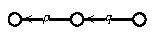
\includegraphics[scale=1.38]{figures/Fig_022_PDF082_Book070.pdf}
  % [Fig] 原书 p.70
\end{figure}
与顶点对应的平凡路径构成一组完全正交幂等元：对所有 $v,w\in Q_0$，
\[
  vw=\begin{cases}
    v,&v=w,\\
    0,&v\ne w,
  \end{cases}
  \qquad\text{并且}\qquad
  \sum_{v\in Q_0}v=1.
\]
\end{definition}

这些幂等元张成半单子代数 $\mathbb C Q_0$。所有非平凡路径张成双边理想
\[
  J=\langle a\mid a\in Q_1\rangle\subset\mathbb C Q.
\]
% [Tutor Note: 乘积顺序务必按"从右到左"：$pq$ 表示先走 $q$ 再走 $p$，所以 $a_1\cdots a_k$ 的拼接条件是 $t(a_i)=h(a_{i+1})$（头尾相接）。若按从左到右理解，后面 $P_v(w)=v\mathbb C Qw$、$\mathbb C Q(v,w)=w\mathbb C Qv$ 和 $vw=\delta_{vw}v$ 的下标会整体反过来。]

\begin{example}[几个基本箭图及其路径代数]\label{ex:basic-quiver-path-algebras}
例如，考虑下面三个箭图：
\begin{figure}[H]\centering
    
\includegraphics[scale=1.38]{figures/Fig_023_PDF083_Book071.pdf}\qquad
    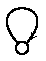
\includegraphics[scale=1.38]{figures/Fig_024_PDF083_Book071.pdf}\qquad
    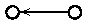
\includegraphics[scale=1.38]{figures/Fig_025_PDF083_Book071.pdf}
  % [Fig] 原书 p.71
\end{figure}
它们对应的路径代数依次为 $\mathbb C$、$\mathbb C[X]$ 和非严格上三角矩阵代数
\[
  \begin{pmatrix}\mathbb C&\mathbb C\\0&\mathbb C\end{pmatrix}.
\]
一个顶点带有 $k$ 个环箭的箭图则给出自由代数 $\mathbb C\langle X_1,\ldots,X_k\rangle$。
\end{example}

\begin{note}\phantomsection\label{note:path-algebra-as-category}
\textbf{注 4.4.} 路径代数也可以看成一个范畴 $\mathbb C Q$。其对象是顶点，两个顶点间的态射空间为
\[
  \mathbb C Q(v,w)=w\mathbb C Qv,
\]
而顶点幂等元就是恒等态射：$1_v=v\in v\mathbb C Qv$。
\end{note}

\subsection{简单模与投射模}\label{subsec:simples-projectives}
分别用 $\mathrm{mod}Q$、$\mathrm{Mod}Q$ 和 $\mathrm{MOD}Q$ 表示有限维、有限生成和所有右 $\mathbb C Q$-模构成的范畴；其 $A_\infty$ 版本分别记作 $\mathrm{mod}^\bullet Q$、$\mathrm{Mod}^\bullet Q$ 和 $\mathrm{MOD}^\bullet Q$。由 $Q_0$ 参数化的两类重要右模为：
\begin{itemize}
  \item 基本投射模\index{jibentoushemo@基本投射模|hyperpage} $P_v=v\mathbb C Q$。它也可看成反变函子
  \[
    P_v\colon\mathbb C Q\to\mathrm{VECT}(\mathbb C),\qquad
    P_v(w)=v\mathbb C Qw,
  \]
  且对箭头 $a$，有 $P_v(a)x=xa$。
  \item 基本简单模\index{jibenjiandanmo@基本简单模|hyperpage} $S_v=v\mathbb C Q/J$。它也可看成反变函子
  \[
    S_v\colon\mathbb C Q\to\mathrm{VECT}(\mathbb C),\qquad
    S_v(w)=\delta_{vw}\mathbb C,
  \]
  且 $S_v(a)=0$。
\end{itemize}

由于前一类模是投射模，它们之间没有非平凡扩张，因此
\[
  \operatorname{Ext}^i_{\mathbb C Q}(P_v,P_w)
  =\begin{cases}
    w\mathbb C Qv,&i=0,\\
    0,&i>0.
  \end{cases}
\]
这说明，导出范畴 $D\mathrm{MOD}^\bullet Q$ 中包含所有基本投射模的全子范畴 $P^\bullet$，同构于集中在次数 $0$、高阶乘积全为零的 $A_\infty$ 范畴 $\mathbb C Q$。

简单模 $S_v$ 有如下投射分解：
\[
  \bigoplus_{h(a)=v}P_{t(a)}\xrightarrow{\,a\cdot\,}P_v.
\]
由此容易算得
\[
  \operatorname{Ext}^i_{\mathbb C Q}(S_v,S_w)=
  \begin{cases}
    \delta_{vw}\mathbb C,&i=0,\\
    \mathbb C^{\oplus\#\{a:v\leftarrow w\}},&i=1,\\
    0,&i>1.
  \end{cases}
\]
% [Tutor Note: $\operatorname{Ext}^1(S_v,S_w)$ 的指标方向最容易写反：它是 $\#\{a:v\leftarrow w\}$，即从 $w$ 指向 $v$ 的箭头数。原因在投射分解 $\bigoplus_{h(a)=v}P_{t(a)}\to P_v$：同调计算给出 $\operatorname{Ext}^1(S_v,S_w)=\operatorname{Hom}(P_{t(a)},S_w)$，只在存在满足 $h(a)=v$、$t(a)=w$ 的箭头时非零。用单箭头箭图 $v_1\to v_2$ 验算：$\operatorname{Ext}^1(S_2,S_1)=\mathbb C$，而 $\operatorname{Ext}^1(S_1,S_2)=0$。]

令 $S=\bigoplus_{v\in Q_0}S_v$。则 $\operatorname{Ext}^\bullet_{\mathbb C Q}(S,S)$ 是一个分次向量空间，由每个顶点 $v\in Q_0$ 对应的次数 $0$ 元素 $v^*=1_{S_v}$ 和每个箭头 $a\in Q_1$ 对应的次数 $1$ 元素 $a^*$ 张成。次数 $0$ 与次数 $1$ 元素之间的乘积顺序反转，因此可把 $v^*$ 和 $a^*$ 看作反向箭图的顶点和箭头。两个次数 $1$ 元素的乘积为零，因为不存在次数 $2$ 的元素。于是得到如下 Ext 环：
\[
  \operatorname{Ext}^\bullet_{\mathbb C Q}(S,S)
  =\mathbb C Q^{\mathrm{op}}/\langle a^*b^*\mid a^*b^*\text{ 是长度为 }2\text{ 的路径}\rangle.
\]
仿照对偶数环（例\ref{ex:dual-numbers-ext}），我们把这个代数称为对偶箭图代数\index{duioujiantudaishu@对偶箭图代数|hyperpage}，记作 $\Lambda_Q$。由于不存在次数 $2$ 的元素，$\Lambda_Q$ 上的高阶乘积全为零。这说明，导出范畴 $D\mathrm{MOD}^\bullet Q$ 中包含所有基本简单模的全子范畴 $S^\bullet$，严格同构于高阶乘积全为零的 $A_\infty$ 范畴 $\Lambda_Q$。

\begin{theorem}{箭图导出范畴的包含关系}{quiver-derived-inclusions}
对任意箭图 $Q$，都有以下 $A_\infty$ 范畴的包含关系：
\[
  DS^\bullet\subset D\mathrm{mod}^\bullet Q\subset DP^\bullet.
\]
若 $Q$ 没有有向圈，则这些包含关系都是等价。
\end{theorem}
\begin{proof}[证明思路]
第一个包含关系显然成立，因为简单模都是一维的。第二个包含关系来自每个模 $M$ 都有如下标准投射分解：
\[
  \bigoplus_{a\in Q_1}M_{h(a)}\otimes_{\mathbb C}P_{t(a)}
  \xrightarrow{\ d\ }
  \bigoplus_{v\in Q_0}M_v\otimes_{\mathbb C}P_v.
\]
在箭头 $a$ 对应的分量上，微分由模作用与路径拼接之差给出：
\[
  d(m_a\otimes x_a)=m_a a\otimes x_a-m_a\otimes ax_a.
\]
若 $M$ 是有限维模，则分解两端都是有限个投射模的直和，因此该分解是 $P^\bullet$ 上的扭曲复形。

当 $Q$ 没有有向圈时，由于路径只有有限多条，基本投射模都是有限维的。此外，简单模只有 $S_v$，而 $\mathbb C Q$（从而所有基本投射模）都由基本简单模生成。因此 $DP^\bullet\subset DS^\bullet$。
\end{proof}

\begin{note}\phantomsection\label{note:quiver-oriented-cycles}
\textbf{注 4.6.} 若 $Q$ 有有向圈，则上述三个范畴两两不同：$DS^\bullet$ 只包含幂零模，即那些经由某个 $\mathbb C Q/J^k$ 因子化的模（$k\geq1$）；而 $D\mathrm{mod}^\bullet Q$ 不包含那些对应顶点位于有向圈上的基本投射模 $P_v$。
\end{note}

\subsection{扭曲复形}\label{subsec:quiver-twisted-complexes}
为在 $D\mathrm{mod}^\bullet Q$、$DP^\bullet$ 和 $DS^\bullet$ 之间方便地转换，我们引入箭图表示\index{jiantubiaoshi@箭图表示|hyperpage}的概念。

\begin{definition}{维数向量与箭图表示}{quiver-representation}
箭图 $Q$ 的维数向量\index{weishuxiangliang@维数向量|hyperpage}是映射 $\alpha\colon Q_0\to\mathbb N$，其大小定义为 $|\alpha|=\sum_{v\in Q_0}\alpha_v$。一个 $\alpha$ 维表示是下列空间的元素：
\[
  \rho\in\operatorname{Rep}(Q,\alpha)
  :=\prod_{a\in Q_1}\operatorname{Mat}_{\alpha_{h(a)}\times\alpha_{t(a)}}(\mathbb C).
\]
\end{definition}

表示 $\rho$ 有三种解释方式：
\begin{itemize}
  \item 它是右 $\mathbb C Q$-模 $M_\rho\colon\mathbb C Q\to\mathrm{vect}(\mathbb C)$：对象 $v$ 映到向量空间 $M_\rho(v):=\mathbb C^{\alpha_v}$，箭头 $a\in Q_1$ 映到线性映射
  \[
    M_\rho(a)\colon\mathbb C^{\alpha_{t(a)}}\to\mathbb C^{\alpha_{h(a)}},
    \qquad x\longmapsto\rho(a)x,
  \]
  其中 $x$ 视为列向量。
  \item 它是 $P^\bullet$ 上的扭曲复形，来自 $M_\rho$ 的标准投射分解：
  \[
    P_\rho=\left(
    \bigoplus_{a\in Q_1}P_{t(a)}^{\oplus\alpha_{h(a)}}
    \xrightarrow{\,\rho(a)-a\,}
    \bigoplus_{v\in Q_0}P_v^{\oplus\alpha_v}
    \right).
  \]
  \item 它是 $S^\bullet$ 上的扭曲复形
  \[
    S_\rho:=\left(\bigoplus_{v\in Q_0}(S_v)^{\oplus\alpha_v},
    \quad \delta=\sum_{a\in Q_1}\rho(a)^\mathsf T a^*\right),
  \]
  其中 $\rho(a)^\mathsf T a^*$ 应看作从 $(S_{h(a)})^{\oplus\alpha_{h(a)}}$ 到 $(S_{t(a)})^{\oplus\alpha_{t(a)}}$ 的矩阵块。由于各个 $a^*$ 之间的乘积都为零，Maurer–Cartan 方程自动成立；但 $\delta$ 未必下三角，所以 $S_\rho$ 未必是扭曲复形。只有当 $M_\rho$ 是幂零模时才是如此。
\end{itemize}

\begin{lemma}{幂零表示对应的扭曲复形}{nilpotent-representation-twisted-complex}
若 $M_\rho$ 是幂零的，则
\[
  S_\rho\simeq M_\rho\simeq P_\rho\in DP^\bullet.
\]
\end{lemma}
\begin{proof}[证明思路]
利用顶点简单模的标准投射分解，可将 $S_\rho$ 变换为 $P_\rho$；再对 $P_\rho$ 取余核，即可得到 $M_\rho$。
\end{proof}

\begin{theorem}{简单模导出范畴的对象分类}{objects-in-derived-simples}
$DS^\bullet$ 中的每个对象都同构于若干个 $S_\rho$ 的移位的直和。
\end{theorem}
\begin{proof}[证明思路]
首先证明每个 $(M,\delta)$ 都同构于这样一个复形：其扭曲项 $\delta$ 中不含顶点恒等态射 $v^*$；对直和项的个数作归纳即可。若只有一个直和项，则 $\delta=0$，结论显然。

取一个扭曲复形 $(M,\delta)$，考察 $\delta$ 的最底行。由归纳假设，可以设 $\delta$ 的其他行只含对偶箭头。共轭变换（见第~\ref{note:conjugation-twisted-complex}~节的注）后，可保证最底行至多出现一个顶点 $v^*=1_{S_v}$。

这个顶点态射连接两个直和项 $S_v[i+1]\xrightarrow{1}S_v[i]$：
\begin{figure}[H]\centering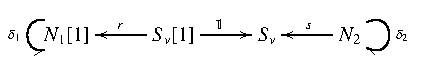
\includegraphics[width=0.72\textwidth]{figures/Fig_026_PDF086_Book074.pdf}
  % [Fig] 原书 p.74
\end{figure}
若 $(M,\delta)$ 不能分解为两个更小复形的直和，则所有其他直和项都通过含对偶箭头的分量与 $S_v[i+1]$ 或 $S_v[i]$ 相连；由于次数限制，它们不可能同时与两者相连。由 $\delta^2=0$ 可知，从 $S_v[i]$ 出发或到达 $S_v[i+1]$ 的分量均为零。于是该复形（相差一个移位）具有图示的形状，并可通过两条拟同构变换为较小复形
\[
  (M_{\mathrm{red}},\delta_{\mathrm{red}})
  =(N_1\oplus N_2[1],\delta_1+\delta_2).
\]
\begin{figure}[H]\centering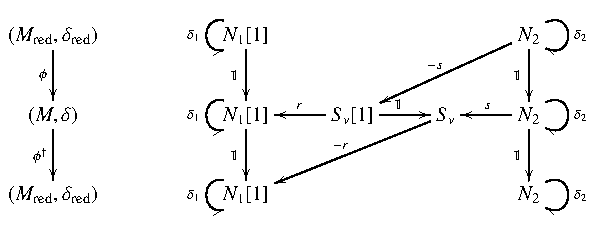
\includegraphics[width=0.94\textwidth]{figures/Fig_027_PDF086_Book074.pdf}
  % [Fig] 原书 p.74
\end{figure}

若一个扭曲复形的 $\delta$ 中只有对偶箭头，则可将其写成所有直和项具有相同移位次数的复形的直和。这样的复形形如 $S_\rho[i]$，其中 $\rho(a)$ 是 $a^*$ 系数构成的矩阵。\end{proof}

\begin{note}\phantomsection\label{note:hereditary-quiver}
\textbf{注 4.10.} 更一般地，可以证明 $D\mathrm{MOD}^\bullet Q$ 中每个对象都同构于若干个模（微分为零的复形）的移位的直和。这是表示论中的经典定理，源于 $\mathbb C Q$ 是遗传代数\index{yichuandaishu@遗传代数|hyperpage}：投射 $\mathbb C Q$-模的子模仍然是投射模。
\end{note}

\section{弦与带}\label{sec:strings-bands}
\takeaway{三种箭图的不可分解对象都有曲线模型：线性箭图 $\leftrightarrow$ $(n+1)$ 边形中的分次线段 $S_{ij}$，克罗内克箭图 $\leftrightarrow$ 圆柱上的弦对象与带对象（后者带秩 $n$ 局部系统），循环箭图 $\leftrightarrow$ 带无穷远端的圆柱上的曲线；态射是交点处的角，乘积由多边形与沿边平行传输给出。}
利用前面建立的形式体系，我们现在考察三个特殊箭图，并将其表示论解释为曲面上线段的交理论。对大多数箭图，不可能分类所有不可分解表示；只有当底层图是 Dynkin 图或扩展 Dynkin 图时，才有完整分类。下面要研究的三个箭图都属于这两类。

\subsection{线性箭图}\label{subsec:linear-quiver}
令 $Q=L_n$ 为有 $n$ 个顶点的线性箭图：
\begin{figure}[H]\centering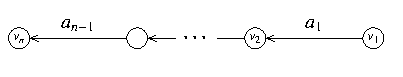
\includegraphics[scale=1.38]{figures/Fig_028_PDF087_Book075.pdf}
  % [Fig] 原书 p.75
\end{figure}
顶点从左到右记作 $v_1,\ldots,v_n$，箭头记作 $a_1,\ldots,a_{n-1}$。顶点简单模记作 $S_i$，对偶箭图中的箭头记作 $\alpha_i=a_i^*$：
\begin{figure}[H]\centering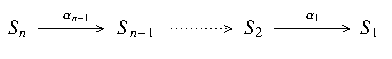
\includegraphics[scale=1.38]{figures/Fig_029_PDF087_Book075.pdf}
  % [Fig] 原书 p.75
\end{figure}

对每一对 $1\leq i\leq j\leq n$，都有一个扭曲复形
\[
  S_{ij}=\left(S_i\oplus\cdots\oplus S_j,
  \delta=\alpha_i+\cdots+\alpha_{j-1}\right).
\]
它对应如下模：顶点 $v_i,\ldots,v_j$ 映到一维向量空间，其间的箭头映到非零映射。等价地，它对应表示 $\rho_{ij}$，其维数向量为
\[
  \varepsilon_{ij}=(0,\ldots,0,1,\ldots,1,0,\ldots,0),
\]
且当 $i\leq k<j$ 时 $\rho_{ij}(a_k)=1$。

\begin{theorem}{线性箭图的不可分解对象}{linear-quiver-indecomposables}
$DS^\bullet$ 中所有不可分解对象都同构于某个 $S_{ij}$ 的移位。
\end{theorem}
\begin{proof}[证明思路]
由定理\ref{thm:objects-in-derived-simples}，$DS^\bullet$ 中每个不可分解对象都是某个 $S_\rho$ 的移位。由于每个对偶顶点恰好有一条 $\alpha_i$ 射出、也恰好有一条 $\alpha_i$ 射入，不可分解的 $S_\rho$ 必须具有如下形式：
\[
  \left(S_i^{\oplus m_i}\oplus S_{i+1}^{\oplus m_{i+1}}
  \oplus\cdots\oplus S_j^{\oplus m_j},
  \quad B_i\alpha_i+\cdots+B_{j-1}\alpha_{j-1}\right),
\]
其中 $B_k$ 是一个元素属于 $\mathbb C$ 的 $m_k\times m_{k+1}$ 矩阵。

将 $\mathbb C^{m_k}$ 分解为 $\operatorname{Im}B_k\oplus R$。若 $R\ne0$，则
\[
  \cdots\oplus B_{k-2}B_{k-1}R\otimes S_{k-2}
  \oplus B_{k-1}R\otimes S_{k-1}\oplus R\otimes S_k
\]
是一个直和项，因此 $B_k$ 必须满射。同理，$B_k$ 也必须单射，否则
\[
  \ker B_k\otimes S_{k-1}\oplus B_{k+1}^{-1}\ker B_k\otimes S_k
  \oplus B_{k+2}^{-1}B_{k+1}^{-1}\ker B_k\otimes S_{k+1}\oplus\cdots
\]
会成为一个直和项。因此所有 $B_k$ 都可逆，并且可通过共轭变换（见第~\ref{note:conjugation-twisted-complex}~节的注）将它们化为单位矩阵。若各矩阵都是 $r\times r$，该扭曲复形便分解为 $r$ 个形如 $S_{ij}$ 的子复形。\end{proof}

确定了不可分解对象之后，下一步是研究它们之间的态射。由定义可得
\[
\begin{aligned}
  \operatorname{Tw}S^\bullet(S_{ij},S_{kl})
  &=\bigoplus_{\substack{i\leq u\leq j<本地路径> u\leq l}}\mathbb C1_{S_u}
  \oplus\bigoplus_{\substack{i\leq v+1\leq j<本地路径> v\leq l}}\mathbb C\alpha_v,
\end{aligned}
\]
其中 $d\alpha_v=0$，而
\[
  d1_{S_u}=\alpha_{u-1}-\alpha_u,
\]
除非 $\alpha_{u-1}$ 或 $\alpha_u$ 不在 $\operatorname{Tw}S^\bullet(S_{ij},S_{kl})$ 中；若不在，就从求和中删去相应项。计算上同调后得到下表。

\begin{lemma}{线性箭图中扭曲复形的态射}{linear-quiver-morphism-table}
设 $S_{ij}$、$S_{kl}$ 是上述扭曲复形，则
\[
\begin{array}{c|c|c}
\text{情形}&DS^0(S_{ij},S_{kl})&DS^1(S_{ij},S_{kl})\\\hline
i-1\leq k-1<j\leq l&\mathbb C\,\iota&0\\
k-1<i-1\leq l<j&0&\mathbb C\,\gamma\\
\text{其他情形}&0&0
\end{array}
\]
次数 $0$ 元素为 $\iota=\sum_u1_{S_u}$，求和遍历两个区间的所有重叠顶点。次数 $1$ 元素为 $\gamma=\alpha_v$（任选一个这样的 $\alpha_v$ 即可；它们在上同调中彼此相等）。
\end{lemma}

这一规则可以从几何角度理解：把扭曲复形看成多边形中的线段。
\begin{definition}{多边形中的分次线段}{graded-line-segment}
取一个正则 $(n+1)$ 边形，顶点为 $p_0,\ldots,p_n$，按逆时针编号，并假设边 $p_np_0$ 是多边形底部的水平边。分次线段\index{fencixianduan@分次线段|hyperpage}是一个二元组 $L=(\overrightarrow{p_ip_j},\theta)$，其中 $\overrightarrow{p_ip_j}$ 是连接两个顶点的有向线段，$\theta\in\mathbb R$ 是相位\index{xiangwei@相位|hyperpage}，满足 $\theta$ 模 $2\pi$ 等于该线段与 $X$ 轴的夹角。

每条 $\overrightarrow{p_ip_j}$ 都可以赋予多个相位，它们相差 $2\pi$ 的整数倍。反转线段方向时，相位必须加上 $\pi$。因此记
\[
  L[k]:=(\overrightarrow{p_jp_i},\theta+k\pi).
\]
每个分次线段都是下列某条线段的移位：
\[
  L_{ij}:=(\overrightarrow{p_{i-1}p_j},\theta),
  \qquad \theta\in(0,2\pi].
\]
\end{definition}

\begin{figure}[H]\centering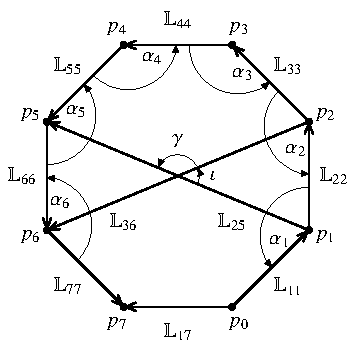
\includegraphics[width=0.95\textwidth]{figures/Fig_030_PDF089_Book077.pdf}
  % [Fig] 原书 p.77
\end{figure}
若把分次线段 $L_{ij}[k]$ 解释为表示 $S_{ij}[k]$，就会看到基本简单模 $S_i=S_{ii}$ 对应多边形的各条边，只有水平底边例外；在图示的八边形情形中，该边对应 $S_{17}$（注意它的定向相反）。两个简单模之间存在次数 $1$ 的态射（扩张），当且仅当对应线段相接。从这一角度看，相应的态射 $\alpha_i$ 就是多边形的角。

这一解释也适用于其他表示。$S_{25}$ 与 $S_{36}$ 之间有两个态射：次数 $0$ 态射 $\iota\colon S_{25}\to S_{36}$；另有次数 $1$ 态射 $\gamma\colon S_{36}\to S_{25}$。从图中可见，线段 $L_{25}$ 和 $L_{36}$ 在多边形内部相交，交点处有两个角，分别朝向两个方向。

\begin{proposition}{观察：态射是角}{morphisms-are-angles}
设 $L_1,L_2$ 是分别对应于分次线段 $(\ell_1,\theta_1)$ 和 $(\ell_2,\theta_2)$ 的两个扭曲复形。若底层线段不同，则
\[
  DS^\bullet(L_1,L_2)\ne0
\]
当且仅当多边形内部存在一个从 $L_1$ 指向 $L_2$ 的正角 $\beta\in[0,\pi)$。此时态射空间由一个次数为
\[
  \frac{\beta-(\theta_2-\theta_1)}{\pi}
\]
的态射生成。该次数衡量转角与相位变化之差。
% [Tutor Note: 次数公式 $\deg=\bigl(\beta-(\theta_2-\theta_1)\bigr)/\pi$ 中 $\beta$ 与 $\theta_i$ 都以逆时针为正；把某个相位换成等价的 $\theta+2\pi$ 不改变次数，但把线段的定向改取相反代表元会同时给 $\beta$ 与 $\theta$ 加 $\pi$，次数保持不变。实践中最容易出错的是只给其中一个量加 $\pi$，结果整体差一次移位。]
\end{proposition}

这种解释也有助于构造锥。再看上图，可以发现：
\begin{itemize}
  \item $\alpha_i\colon S_{i+1}\to S_i$ 的锥为 $S_{i,i+1}$，几何上可看成用角 $\alpha_i$ 将 $S_i$ 和 $S_{i+1}$ 对应的线段拼接，再将拐角拉直。
  \item $\gamma\colon S_{36}\to S_{25}$ 的锥为
  \[
    \left(S_2\oplus S_3\oplus S_4\oplus S_5
    \oplus S_3\oplus S_4\oplus S_5\oplus S_6,
    \alpha_3+\alpha_4+\alpha_5+\alpha_4+\alpha_5+\alpha_6+\gamma\right).
  \]
  重新排列后，它同构于 $S_{26}\oplus S_{35}$。从几何上看，我们使用角 $\gamma$ 以另一种方式拼接线段。
  \item 把次数 $1$ 态射 $\iota\colon S_{25}\to S_{36}$ 看成 $\iota\colon S_{25}[1]\to S_{36}$，取其锥可得
  \[
    \left(S_2[1]\oplus\cdots\oplus S_5[1]\oplus S_3\oplus\cdots\oplus S_6,
    -\alpha_3-\alpha_4-\alpha_5+\alpha_4+\alpha_5+\alpha_6
    +1_{S_3}+1_{S_4}+1_{S_5}\right),
  \]
  由定理\ref{thm:objects-in-derived-simples}的证明方法可知，它同构于 $S_2[1]\oplus S_6$。这里同样是利用角把线段拼接起来。
\end{itemize}

\begin{proposition}{观察：锥是拼接}{cones-are-stitches}
设 $L_1,L_2$ 是相位属于 $(0,2\pi)$ 的两条分次线段，$\alpha$ 是对应于次数 $1$ 态射的角。取 $\alpha$ 的锥，在几何上就是沿着 $\alpha$ 将两条线段拼接所得的线段。
\end{proposition}
\begin{figure}[H]\centering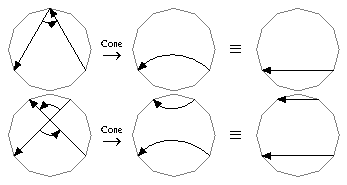
\includegraphics[width=0.78\textwidth]{figures/Fig_031_PDF090_Book078.pdf}
  % [Fig] 原书 p.78
\end{figure}

几何解释的最后一部分涉及乘积。位于多边形同一顶点的边界角相乘时，会合成为一个角；那么内部角又如何相乘？我们再看两个例子。
\begin{itemize}
  \item 取扭曲复形 $A=S_{36}$、$B=S_{25}$、$X=S_{47}$、$Y=S_{35}$。有次数 $0$ 态射 $\iota_{AX}\colon S_{36}\to S_{47}$ 和次数 $1$ 态射 $\gamma_{XB}\colon S_{47}\to S_{25}$。它们的复合是次数 $1$ 态射 $\gamma_{AB}\colon S_{36}\to S_{25}$。从图中可见，$\iota_{AX}$ 和 $\gamma_{XB}$ 是一个三角形的内部角，而 $\gamma_{AB}$ 是第三个顶点处的外角。
  \item $\iota_{BY}\colon S_{25}\to S_{35}$ 与 $\iota_{YA}\colon S_{35}\to S_{36}$ 的乘积是 $\iota_{BA}\colon S_{25}\to S_{36}$；后者是以 $\iota_{BY}$ 和 $\iota_{YA}$ 为内角的三角形在第三个顶点处的外角。
\end{itemize}
\begin{figure}[H]\centering
  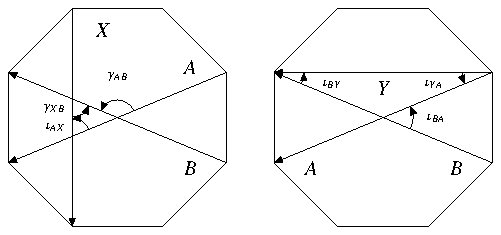
\includegraphics[width=0.44\textwidth]{figures/Fig_032_PDF091_Book079.pdf}\hfill
  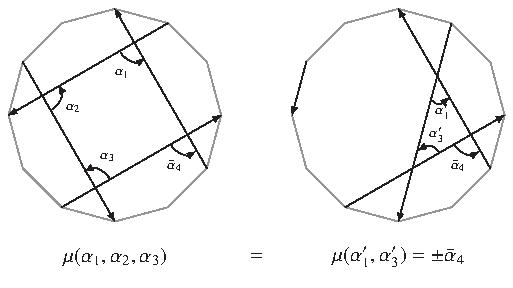
\includegraphics[width=0.44\textwidth]{figures/Fig_033_PDF091_Book079.pdf}
  % [Fig] 原书 p.79
\end{figure}

因此，乘积对应三角形。这一观察甚至可推广到高阶乘积。若有一个内部 $n$ 边形，想要对其中 $n-1$ 个内部角取高阶乘积，就可以对其中一个态射取锥，把问题改写为 $(n-2)$ 元乘积（见引理\ref{lem:higher-products-and-cones}）。取锥会把两条边拼在一起，形成一个 $(n-2)$ 边形。重复这一过程，最后得到一个三角形，便可用二元乘积规则解释：
\[
  \mu(\alpha_1,\alpha_2,\alpha_3)
  =\mu(\alpha'_1,\alpha'_3)=\pm\overline\alpha_4.
\]
\begin{figure}[H]\centering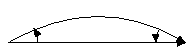
\includegraphics[width=0.72\textwidth]{figures/Fig_034_PDF092_Book080.pdf}
  % [Fig] 原书 p.80
\end{figure}

\begin{proposition}{观察：多边形诱导乘积}{polygons-induce-products}
若 $L_1,\ldots,L_k$ 是围成一个子多边形的线段，则除一个角以外，所有连接这些线段的内部态射的高阶乘积，等于剩余顶点处的外角态射：
\[
  \mu(\alpha_1,\ldots,\alpha_{k-1})=\pm\overline\alpha_k.
\]
符号取决于这些态射的次数。
\end{proposition}

\begin{note}\phantomsection\label{note:degenerate-polygons}
\textbf{注 4.17.} 请注意，$DS^\bullet$ 中并非每个非零乘积都来自一个多边形，因为有时对应的多边形会退化（例如三条线段经过同一点，或其中若干线段重合）。
\end{note}

\begin{proposition}{观察：线段交理论}{intersection-theory-line-segments}
$A_\infty$ 范畴 $DS^\bullet$ 描述了多边形中线段的交理论。
\end{proposition}

\begin{note}\phantomsection\label{note:rigorous-polygon-model}
\textbf{注 4.19.} 要使这一观察严格化并不容易。一种办法是使用预范畴，定义如下：
\begin{itemize}
  \item 横截序列是所有两两交点彼此不同的分次线段序列；
  \item Hom 空间是由交点处各个角张成的分次 $\mathbb C$-向量空间；
  \item 唯一可能非零的乘积由观察\ref{pro:polygons-induce-products}中的规则给出。
\end{itemize}
遗憾的是，这个预范畴没有同构。为解决这一问题，可以加入分次曲线\index{fenciquxian@分次曲线|hyperpage}。分次曲线是一个二元组
\[
  L=\bigl(\gamma\colon[0,1]\to\mathbb R^2,
  \theta\colon[0,1]\to\mathbb R\bigr),
\]
其中 $\gamma$ 是多边形内连接两个不同顶点的光滑嵌入，而 $\theta(x)$ 是 $\gamma$ 在 $x$ 处的切向量与 $X$ 轴的夹角。

在这个预范畴中，图示的角都是拟同构：
\begin{figure}[H]\centering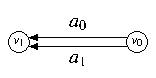
\includegraphics[width=0.52\textwidth]{figures/Fig_035_PDF093_Book081.pdf}
  % [Fig] 原书 p.81
\end{figure}
因此相应的极小模型 $\mathrm{Polygon}_{n+1}^\bullet$ 是一个具有足够多同构的预范畴。将其范畴化后，得到等价
\[
  DS^\bullet\cong_\infty\mathrm{Polygon}_{n+1}^\bullet.
\]
\end{note}

\subsection{克罗内克箭图}\label{subsec:kronecker-quiver}
接下来考察克罗内克箭图 $Q=K$。它由两个顶点 $v_0,v_1$ 和两条方向相同的箭头 $a_0,a_1$ 组成：
\begin{figure}[H]\centering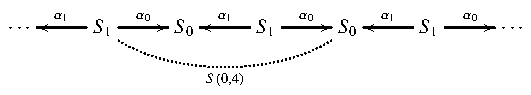
\includegraphics[width=0.28\textwidth]{figures/Fig_036_PDF093_Book081.pdf}
  % [Fig] 原书 p.81
\end{figure}

范畴 $P^\bullet$ 包含两个投射模 $P_i=v_i\mathbb C Q$，范畴 $S^\bullet$ 包含两个简单模 $S_i=v_i\mathbb C Q/\langle a_0,a_1\rangle$。这两个简单模的 Ext 环是 $\Lambda_Q$。由于不存在长度为 $2$ 的路径，$\mathbb C Q^{\mathrm{op}}\cong\mathbb C Q$。因此，范畴 $S^\bullet$ 和 $P^\bullet$ 看起来相同，但分次不同：$P^\bullet$ 中所有态射的次数都是 $0$，而 $S^\bullet$ 中对偶箭头 $\alpha_i=a_i^*$ 的次数为 $1$。

\begin{theorem}{克罗内克箭图的不可分解对象}{kronecker-quiver-indecomposables}
$DS^\bullet$ 中每个不可分解对象都同构于下列复形之一的移位：
\begin{enumerate}[label=(\roman*)]
  \item $S(i,w)$ 是下方无穷串中的一个线性子复形，它从右侧的 $S_i$ 开始，共含 $w$ 项；
  \begin{figure}[H]\centering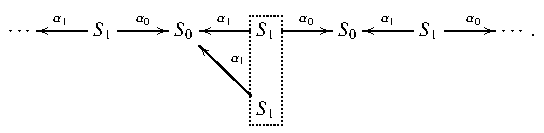
\includegraphics[width=0.91\textwidth]{figures/Fig_037_PDF094_Book082.pdf}
  % [Fig] 原书 p.82
\end{figure}
  \item
  \[
    B(\lambda,n)=\left(S_0^{\oplus n}
    \xleftarrow{\,\alpha_0 1_n+\alpha_1J(\lambda,n)\,}
    S_1^{\oplus n}\right),
  \]
  其中 $J(\lambda,n)$ 是大小为 $n$、特征值为 $\lambda\in\mathbb C^*$ 的 Jordan 块。
\end{enumerate}
\end{theorem}
\begin{proof}[证明思路]
设 $(M,\delta)$ 是一个不可分解扭曲复形。由定理\ref{thm:objects-in-derived-simples}，可设它具有如下形式：
\[
  \left(S_0[k]^{\oplus n}\oplus S_1[k]^{\oplus m},
  \quad B_0\alpha_0+B_1\alpha_1\right),
\]
其中 $B_0,B_1$ 是 $m\times n$ 矩阵。相差一个同构，我们可以分别在左、右乘同一个可逆矩阵。若 $B_0,B_1$ 都可逆，则可先把 $B_0$ 化为单位矩阵，再将 $B_1$ 共轭化为 Jordan 块，从而得到 $B(\lambda,n)$。

若 $B_0$ 或 $B_1$ 不可逆，则对 $n+m$ 作归纳，证明 $(M,\delta)$ 同构于某个 $S(i,w)$。当 $n+m=1$ 时，$(M,\delta)$ 显然是 $S_0=S(0,1)$ 或 $S_1=S(1,1)$。当 $n+m\geq2$ 时，根据 $B_i$ 是否单射、是否满射分为四种情形；这里只详述其中一种。

假设 $B_0$ 有核。取核中的一个基向量 $v$，并令 $w=B_1v$。由于扭曲复形不可分解，$w\ne0$。将 $v,w$ 分别扩充为 $\mathbb C^n$ 与 $\mathbb C^m$ 的基，可以把两个矩阵写成如下形式：
\[
  B_0=\begin{pmatrix}0&*\\0&B'_0\end{pmatrix},
  \qquad B_1=\begin{pmatrix}1&*\\0&B'_1\end{pmatrix}.
\]
通过右乘可逆矩阵，可以假定 $B_1$ 的第一行以零开头。由于 $B'_1$ 不可逆，$(B'_0,B'_1)$ 满足归纳假设，因而对应某个弦对象\index{xianduixiang@弦对象|hyperpage} $S(i,w)$。原复形于是具有原书图示的串形结构。

若最底下的 $S_1$ 在链的中部与其他项相连，则考察 $B_0,B_1$ 在虚线所示 $S_1\oplus S_1$ 上限制所得的核 $K_0,K_1$。若二者相同，则有一个同构于 $S_1$ 的直和项；若它们张成 $K_0\oplus K_1=S_1\oplus S_1$，则整个复形可拆成两个复形的直和：
\begin{figure}[H]\centering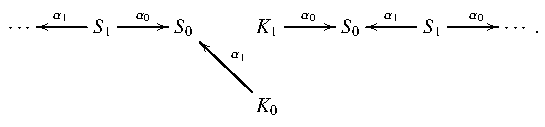
\includegraphics[width=0.91\textwidth]{figures/Fig_038_PDF094_Book082.pdf}
  % [Fig] 原书 p.82
\end{figure}
因此，在不可分解情形下，该 $S_1$ 必须连到链的一端，故整个对象就是一条链。\end{proof}

\begin{definition}{弦对象与带对象}{string-and-band-objects}
我们称 $S(i,w)$ 为弦对象，称 $B(\lambda,n)$ 为带对象\index{daiduixiang@带对象|hyperpage}。
\end{definition}

\begin{note}\phantomsection\label{note:strings-as-band-limits}
\textbf{注 4.22.} 长度为偶数的弦对象可视为带对象的极限：
\[
  \lim_{\lambda\to0}B(\lambda,n)\cong S(0,2n),
  \qquad
  \lim_{\lambda\to\infty}B(\lambda,n)\cong S(1,2n).
\]
第一个极限可直接从复形图中看出。对于第二个极限，注意到经过基变换，可以把映射 $\alpha_0 1_n+\alpha_1J(\lambda,n)$ 化为 $\alpha_0J(\lambda^{-1},n)+\alpha_1 1_n$。因此，我们有时也把这些弦对象记作 $B(0,n)$ 和 $B(\infty,n)$。
% [Tutor Note: 何以"偶长弦对象是带对象的极限"：$\lambda\to0$ 时 $J(\lambda,n)\to J(0,n)$ 成为幂零块，$\alpha_01_n+\alpha_1J(0,n)$ 的秩使复形退化为 $2n$ 项的一维链；$\lambda\to\infty$ 时首项与末项互换，得到方向相反的 $S(1,2n)$。因此带对象在参数边界上退化为偶长弦对象；对 $\lambda\in\mathbb C^*$，带对象与弦对象是不同的不可分解对象。]
\end{note}

现在为克罗内克箭图构造类似于线性箭图情形的几何解释。取一个正方形，把左右两边粘合，便得到一个圆柱；正方形的两个角分别给出圆柱两条边界圆上的标记点。圆柱是平坦曲面，可以通过提升到正方形按通常方式测量角度。与多边形情形一样，也可以定义标记点之间的分次线段。

令 $S_0$ 表示对应于正方形竖边、相位为 $\frac\pi2$ 的分次线段；令 $S_1$ 表示相位为 $\frac{5\pi}4$、方向向下的对角线。由 $S_1$ 指向 $S_0$ 有两个角，它们分别对应 $S_1$ 与 $S_0$ 之间的两个次数 $1$ 态射：
\begin{figure}[H]\centering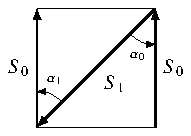
\includegraphics[width=0.56\textwidth]{figures/Fig_039_PDF095_Book083.pdf}
  % [Fig] 原书 p.83
\end{figure}

在线性箭图的多边形模型中，我们已把取锥解释为沿一个角拼接线段。同样，每个弦对象 $S(i,w)$ 都可看成圆柱普遍覆盖空间中的一条线段：
\begin{figure}[H]\centering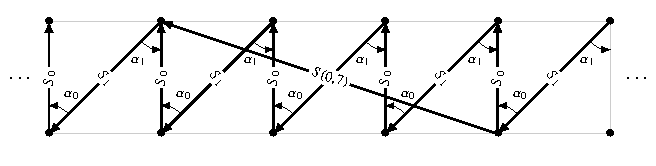
\includegraphics[width=0.96\textwidth]{figures/Fig_040_PDF095_Book083.pdf}
  % [Fig] 原书 p.83
\end{figure}

带对象又如何解释？还有另一类相位恒定的曲线：绕圆柱一周的圆。若要用这些圆解释带对象，还需附加几何数据，即局部系统\index{jubuxitong@局部系统|hyperpage}。

\begin{definition}{局部系统}{local-system}
流形 $M$ 上的局部系统是其基本群胚的一个表示
\[
  L\colon\Pi_1(M)\to\mathrm{vect}(\mathbb C).
\]
局部系统 $L$ 给每个点 $p$ 配一个向量空间 $L(p)$，称为 $p$ 上的纤维；对任意两个点之间每条路径的同伦类，还给出这些向量空间之间的一个可逆映射，有时称为沿该路径的平行传输。若 $M$ 连通，则所有纤维维数相同，称为局部系统的秩\index{zhi@秩|hyperpage}。
\end{definition}

\begin{lemma}{圆上的不可分解局部系统}{indecomposable-local-systems-circle}
圆周 $S^1$ 上的不可分解局部系统由可逆 Jordan 块分类。
\end{lemma}
\begin{proof}[证明思路]
圆周的基本群胚等价于群 $\mathbb Z$。因此，同构意义下，一个表示 $\varphi\colon\mathbb Z\to\mathrm{GL}_n$ 由可逆矩阵 $\varphi(1)$ 的共轭类确定，而该矩阵可化为 Jordan 标准形。
\end{proof}

在圆柱中固定一条水平圆，则每个带对象 $B(n,\lambda)$ 都可与这条圆上的一个局部系统对应；沿圆周的平行传输由大小为 $n$、特征值为 $\lambda$ 的 Jordan 块给出。我们把嵌入的圆及其局部系统一并记作 $B(n,\lambda)$。

弦对象也可以看成带有秩 $1$ 局部系统的线段。可缩空间上的局部系统由其秩分类，而秩为 $n$ 的局部系统是 $n$ 个秩 $1$ 局部系统的直和。因此，$S_0\oplus S_0$ 既可以看成两条各带秩 $1$ 局部系统的线段，也可以看成一条带秩 $2$ 局部系统的线段。今后默认每条分次线段 $L$ 都带有一个局部系统，并用 $L(p)$ 表示 $p$ 处的纤维。

为处理这些局部系统，还需升级态射空间。交点 $p$ 周围的每个角都应看成两个局部系统在 $p$ 处纤维之间的一个态射。因此，若 $L_1,L_2$ 是分别位于两条不同线段上的局部系统，则令
\[
  \operatorname{Hom}(L_1,L_2)
  =\bigoplus_{\alpha_p}\mathrm{vect}(L_1(p),L_2(p))_{\alpha_p},
\]
其中 $\alpha_p$ 表示交点 $p$ 处的一个角。换言之，每个角都带有一个线性映射作为系数。

这一想法与取锥构造相容。若要用态射 $f\alpha_p$ 将两个局部系统拼接起来，其中 $f\colon L_1(p)\to L_2(p)$ 可逆，就用 $f$ 识别两处纤维。若 $f$ 不可逆，则将局部系统分解为 $f$ 可逆的部分和 $f$ 为零的部分，只拼接前一部分。

带对象 $B(n,\lambda)$ 可看成分别位于 $S_0$ 和 $S_1$ 上的两个秩为 $n$ 的局部系统：一端用恒等映射拼接，另一端用 Jordan 块拼接。合起来得到一条与圆同伦的曲线，其局部系统的平行传输恰好等于该 Jordan 块；这就是 $B(n,\lambda)$。

最后还需调整乘积规则。乘积中的角系数必须双线性地纳入乘积，但连续相乘的角并不连接同一个交点处的纤维，所以这些线性映射无法直接相乘。局部系统可以解决这一问题。若多边形的一条边 $e\colon p\to q$ 位于 $L_i$ 上，则局部系统给出纤维间的映射
\[
  L_i(e)\colon L(p)\to L(q).
\]
于是可以把这些映射串接起来，定义扩展乘积：
\[
\begin{aligned}
  \mu(f_1\alpha_1,\ldots,f_4\alpha_4)
  ={}&L_1(e_0)f_1L_1(e_1)\cdots L_1(e_3)f_4L_k(e_4)\cdot\overline\alpha_0\\
    &+\cdots.
\end{aligned}
\]
\begin{figure}[H]\centering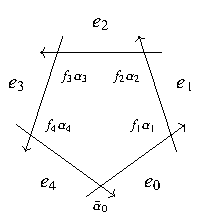
\includegraphics[width=0.58\textwidth]{figures/Fig_041_PDF097_Book085.pdf}
  % [Fig] 原书 p.85
\end{figure}
若这些角围成不止一个多边形，就把相应表达式求和。加入这些结构后，可以验证，线性箭图情形中对 $DS^\bullet$ 的观察同样适用于克罗内克箭图。

\begin{proposition}{观察：局部系统与多边形乘积}{local-systems-and-polygon-products}
$DS^\bullet$ 中的对象可识别为带有局部系统的分次线段的直和。态射是由局部系统纤维间映射加权的角；多边形对乘积的贡献，则由沿边界的总平行传输加权。
\end{proposition}

\subsection{循环箭图}\label{subsec:cyclic-quiver}
最后考察循环箭图 $Q=C_n$。它有 $n$ 个顶点 $v_1,\ldots,v_n$ 和 $n$ 条箭头 $a_i\colon v_i\to v_{i+1}$，下标按模 $n$ 计算：
\begin{figure}[H]\centering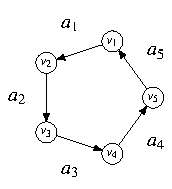
\includegraphics[width=0.48\textwidth]{figures/Fig_042_PDF097_Book085.pdf}
  % [Fig] 原书 p.85
\end{figure}

我们允许 $n=1$，此时箭图只有一个顶点和一个环箭。范畴 $P^\bullet$ 中有 $n$ 个投射模 $P_i=v_i\mathbb C Q$，范畴 $S^\bullet$ 中有 $n$ 个简单模 $S_i=v_i\mathbb C Q/J$。对偶箭头 $\alpha_i=a_i^*$ 是从 $S_{i+1}$ 到 $S_i$ 的次数 $1$ 态射。

情形与前两个例子略有不同：由于存在任意长度的路径，$\mathbb C Q$ 是无限维的。取所有长度为 $n$ 的路径之和，可得 $\mathbb C Q$ 中的一个中心元素，记作
\[
  \ell=a_n\cdots a_1+a_1a_n\cdots a_2+\cdots
  +a_{n-1}\cdots a_1a_n.
\]
容易验证，$\mathbb C[\ell]$ 是多项式环，而 $\mathbb C Q$ 是一个自由 $\mathbb C[\ell]$-模，其基由所有长度小于 $n$ 的路径组成。由于 $\mathbb C Q$ 是无限维的，三个范畴
\[
  DS^\bullet\subset D\mathrm{mod}^\bullet Q\subset DP^\bullet
\]
彼此不同；分类定理也体现了这一点。

\begin{theorem}{循环箭图投射导出范畴中的不可分解对象}{cyclic-quiver-projective-indecomposables}
$DP^\bullet$ 中的不可分解对象都是下列对象之一的移位：
\begin{itemize}
  \item
  \[
    S(i,w)=\left(S_i\oplus\cdots\oplus S_{i+w-1},
    \alpha_i+\cdots+\alpha_{i+w-1}\right);
  \]
  \item $B(k,\lambda)=M_\rho$，其中 $\rho(a_n)=J(k,\lambda)$，且对 $i\ne n$ 有 $\rho(a_i)=1_k$；
  \item $P_i$。
\end{itemize}
这里 $i\in\{1,\ldots,n\}$、$\lambda\in\mathbb C$、$w\in\mathbb N$。并且
\[
  S(i,w)\in DS^\bullet,\qquad
  B(k,\lambda)\in D\mathrm{mod}^\bullet Q,\qquad
  P_i\in DP^\bullet.
\]
\end{theorem}
\begin{proof}[证明思路]
$DP^\bullet$ 中每个不可分解对象都是一个有限生成 $\mathbb C Q$-模 $M$ 的移位。若 $M$ 是无限维的，则存在单射 $P_v\to M$；由于 $P_v$ 是投射模，该单射分裂，因此 $M\cong P_v$。

若 $M$ 是有限维的，则 $M=M_\rho$。由于 $\ell$ 是中心元，可按 $\ell$ 的特征值将 $M$ 分解为直和。因此，不可分解情形下 $\ell$ 只有一个特征值 $\lambda$。若 $\lambda\ne0$，则所有 $\rho(a_i)$ 都可逆；通过共轭，可将除 $\rho(a_n)$ 之外的矩阵化为单位矩阵，而 $\rho(a_n)$ 可化为 Jordan 块。若 $\lambda=0$，则该模是幂零模，因而属于 $DS^\bullet$。最后仿照定理\ref{thm:kronecker-quiver-indecomposables}的论证即可完成分类。
\end{proof}

这一分类同样可以解释为曲面上的曲线。取一个圆盘，中心有一个标记点，边界上有 $n$ 个标记点。把 $n$ 个简单对象对应到边界上逆时针排列的 $n$ 条弧，把 $n$ 个投射对象对应到由中心向外辐射的线段。对象 $B(k,\lambda)$ 则对应绕中心一周、并带有平行传输为 $J(k,\lambda)$ 的局部系统的曲线：
\begin{figure}[H]\centering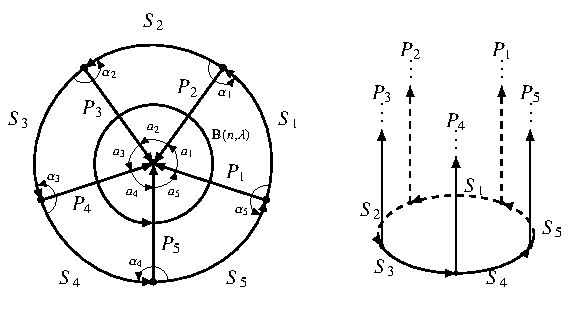
\includegraphics[width=0.92\textwidth]{figures/Fig_043_PDF099_Book087.pdf}
  % [Fig] 原书 p.87
\end{figure}

箭图的箭头对应投射模之间的态射，可看成中心标记点周围的角；对偶箭头在简单模之间给出态射，可看成圆周标记点附近的角。

乍看之下，一切都吻合，除了分次：若在欧氏平面中测量角度，则从 $P_1$ 到自身的态射 $a_n\cdots a_1$ 绕转 $2\pi$，因而必须有次数 $2$。解决办法是把曲面看成带有一个无穷远端的圆柱，而不是圆盘。此时各线段 $P_i$ 的相位为 $\frac\pi2$，而 $S_i$ 的相位为 $0$。由 $S_i,P_i,P_{i+1}$ 围成的三角形有两个 $\frac\pi2$ 的角和一个位于无穷远处的零角。

\begin{proposition}{观察：循环箭图的曲线模型}{cyclic-quiver-curves}
循环箭图的表示论可用带有一个无穷远端的圆柱上的曲线来解释。范畴 $DS^\bullet$ 包含位于边界圆上的线段，$D\mathrm{mod}^\bullet Q$ 包含紧致线段（即不延伸到无穷远处的线段），而 $DP^\bullet$ 还包含非紧致线段。
\end{proposition}

\section{点与层}\label{sec:points-sheaves}
\takeaway{同一批箭图也可解释为代数几何对象：单环箭图 $\leftrightarrow$ $\mathbb A^1$ 上的相干层，循环箭图 $\leftrightarrow$ 轨形 $[\mathbb A^1/\mathbb Z_n]$ 上的相干层（叉积代数 $\mathbb C[X]\star G$ 的模），克罗内克箭图 $\leftrightarrow$ $\mathbb P^1$ 上相干层（用两片 $\mathbb A^1$ 加粘合数据描述），线性箭图 $\leftrightarrow$ Landau--Ginzburg 模型的奇点范畴。}
本节将从另一种几何视角，即代数几何，回顾前三种箭图，并按与前面相反的顺序逐一讨论。

\subsection{循环箭图}\label{subsec:cyclic-quiver-sheaves}
先从只有一个环箭的箭图开始。它的路径代数是多项式环 $R=\mathbb C[X]$。这个环可以看成仿射直线 $\mathbb A^1=\mathbb C$ 上的多项式函数环。对每个点 $p\in\mathbb C$，有一个映射
\[
  \rho_p\colon R\to\mathbb C,\qquad f(X)\longmapsto f(p),
\]
它把每个函数取值于点 $p$。其核为
\[
  \mathfrak p=\{f\in R\mid f(p)=0\}=(X-p),
\]
模去这个核便得到简单模 $S_p=J(p,1)$。所有简单模都可如此得到，因此
\[
  \{\mathbb A^1\text{ 上的点}\}
  \longleftrightarrow\{R\text{ 的极大理想}\}
  \longleftrightarrow\{R\text{ 的简单模}\}.
\]

高阶 Jordan 块也有类似解释：$\rho_p$ 把每个函数映到它在 $p$ 处的函数值，而映射
\[
  R\to J(p,n)=\mathbb C[X]/(X-p)^n
\]
则把每个 $f$ 映到它在 $p$ 处的 $n$ 阶 Taylor 近似。因此，$J(p,n)$ 探测了点 $p$ 的无穷小邻域。

若 $M/\mathfrak pM\ne0$，则称模 $M$ 的支撑包含点 $p\in\mathbb A^1$。显然，$S_p$ 只支撑在 $p$，不支撑在其他点 $q$；$J(p,n)$ 也一样。但若把 $R$ 看成它自身上的模，情形就不同了：它在每个 $p$ 处都有支撑。每一点上的商空间 $R/\mathfrak p$ 都是一维向量空间，把这些空间合在一起，便得到 $\mathbb A^1$ 上的一个一维向量丛（或线丛\index{xiancong@线丛|hyperpage}）。$R$ 中每个元素 $m$ 在每个点 $p$ 上都给出 $R/\mathfrak p$ 中的一个元素，因此可看作该向量丛的截面。这个线丛是平凡的，因为元素 $1\in R$ 给出一个截面，并在每个纤维中构成一组基。由于 $\mathbb A^1$ 可缩，其上的每个向量丛都是平凡的；秩为 $n$ 的向量丛对应于投射（事实上自由）模 $R^{\oplus n}$：
\[
  \{\mathbb A^1\text{ 上的向量丛}\}
  \longleftrightarrow\{\text{投射 }R\text{-模}\}.
\]

既非投射模也非简单模的模有更精细的几何解释，称为相干层。第七章将更详细地讨论这一概念；目前只需知道，$\mathbb A^1$ 上的相干层等同于有限生成 $\mathbb C[X]$-模：
\[
  D\mathrm{Coh}^\bullet\mathbb A^1
  =D\mathrm{Mod}^\bullet\mathbb C[X].
\]

\begin{proposition}{观察：单环箭图与仿射直线上的层}{one-loop-quiver-sheaves}
单环箭图的表示可解释为仿射直线 $\mathbb A^1$ 上的层。在这一对应下，简单模 $S_p$ 变为支撑在点 $p$ 上的零维层，称为点层\index{dianceng@点层|hyperpage}；自由模 $\mathbb C[X]$ 变为平凡线丛 $\mathcal O$，也称结构层\index{jiegouceng@结构层|hyperpage}。
\end{proposition}

现在把这一几何解释推广到更高阶循环箭图。仍取仿射直线 $\mathbb A^1$，令循环群
\[
  G=\langle g\mid g^n=1\rangle\cong\mathbb Z_n
\]
左作用于其上：
\[
  g^k\cdot x=\zeta^kx,
  \qquad \zeta=e^{2\pi i/n}.
\]
除原点轨道只含一个点外，其余轨道都含 $n$ 个点。该作用诱导坐标环 $\mathbb C[X]$ 上的右作用，定义为
\[
  f\cdot g(x)=f(g\cdot x).
\]
若要取商，$\mathbb A^1/G$ 的坐标环应看作 $G$-不变函数环 $\mathbb C[X]^G$，因为不变函数在每个轨道上取值相同。这个环是 $\mathbb C[X^n]$，与 $\mathbb C[X]$ 同构，所以从这一角度看，$\mathbb A^1/G$ 似乎与 $\mathbb A^1$ 相同。

然而，这并未充分反映几何，因为 $\mathbb A^1/G$ 有一个特殊点（原点），而 $\mathbb A^1$ 上所有点看起来都相同。因此，更合适的做法是把商看成更精细的对象——轨形 $[\mathbb A^1/G]$，而不是仿射簇。

为此，引入 $G$-等变层：它是 $\mathbb A^1$ 上的一个层，并带有一个与 $G$ 在 $\mathbb A^1$ 上的作用相容的 $G$-作用。更精确地说，它是一个带 $G$-作用的 $\mathbb C[X]$-模 $M$，满足
\[
  (mf(x))\cdot g=(m\cdot g)(f(x)\cdot g).
\]
这两个作用可以合并到一个代数中：
\[
  \mathbb C[X]\star G
  :=\mathbb C\langle X,g\rangle
  /\langle gXg^{-1}-\zeta X,\ g^n-1\rangle.
\]
于是 $M$ 自然成为一个 $\mathbb C[X]\star G$-模。因此，定义 $G$-等变相干层的导出范畴
\[
  D\mathrm{Coh}^\bullet[\mathbb A^1/\mathbb Z_n]
  :=D\mathrm{Mod}^\bullet(\mathbb C[X]\star G).
\]
% [Tutor Note: 关系 $gXg^{-1}=\zeta X$ 说明 $g$ 并不固定 $X$，而是把 $X$ 的本征值旋转 $\zeta$；因此 $\mathbb C[X]\star G$ 比不变环 $\mathbb C[X]^G=\mathbb C[X^n]$ 大得多，前者的模保留了 $G$ 在纤维上的作用，这正是"轨形"与"商簇"的差别所在。$g^n=1$ 与 $gXg^{-1}=\zeta X$ 相容，因为 $\zeta^n=1$。]
这个范畴是轨形 $[\mathbb A^1/G]$ 上层范畴的合适替代，因此应把 $D\mathrm{Coh}^\bullet[\mathbb A^1/G]$ 视作 $[\mathbb A^1/G]$ 上相干层的导出范畴。

\begin{theorem}{循环箭图路径代数与叉积代数}{cyclic-quiver-crossed-product}
代数 $\mathbb C[X]\star G$ 同构于 $Q$ 为 $n$ 个顶点循环箭图时的路径代数 $\mathbb C Q$。
\end{theorem}
\begin{proof}[证明思路]
令 $\zeta=e^{2\pi i/n}$，并定义
\[
  e_k=\frac1n\sum_{i=1}^n\zeta^{ki}g^i.
\]
容易验证 $\sum_k e_k=1$ 且 $e_ie_j=\delta_{ij}e_i$。也就是说，这些元素构成一组正交幂等元。此外，
\[
  Xe_k=e_{k+1}X,
  \qquad
  X=\sum_i e_{i+1}Xe_i,
\]
下标均按模 $n$ 计算。现定义态射 $\varphi\colon\mathbb C Q\to\mathbb C[X]\star G$，把顶点映为 $e_k$，把箭头 $a_i$ 映为 $e_{i+1}Xe_i$。容易验证，$\varphi$ 是同构。
\end{proof}

\begin{proposition}{观察：循环箭图与轨形上的相干层}{cyclic-quiver-orbifold-sheaves}
循环箭图的表示论可以几何地解释为轨形上的相干层：
\[
  D\mathrm{Coh}^\bullet[\mathbb A^1/G]
  \cong_\infty D\mathrm{Mod}^\bullet\mathbb C C_n.
\]
\end{proposition}

\subsection{克罗内克箭图}\label{subsec:kronecker-quiver-sheaves}
为了给克罗内克箭图构造类似的解释，需要考察射影直线的代数几何。射影直线是在仿射直线 $\mathbb A^1$ 上添加一个无穷远点：$\mathbb P^1=\mathbb A^1\cup\{\infty\}$。用齐次坐标也可表示为
\[
  \mathbb P^1:=\{(x:y)\mid(x,y)\in\mathbb C^2\setminus\{(0,0)\}\},
\]
其中 $(x:y)$ 与其任意非零数倍 $(\lambda x:\lambda y)$ 视为相同。它可看成两条仿射直线
\[
  \{(x:1)\mid x\in\mathbb C\},\qquad
  \{(1:y)\mid y\in\mathbb C\}
\]
的并集，它们的交集为 $\mathbb C^*$。

这两条仿射直线的坐标环分别为 $R_X=\mathbb C[X]$ 和 $R_Y=\mathbb C[Y]$。在交叠处，$X,Y$ 都可视为函数，且满足 $Y=X^{-1}$。交叠部分的坐标环为
\[
  R_{XY}=\mathbb C[X,Y]/(XY-1).
\]
另一方面，$\mathbb C[X]$ 与 $\mathbb C[Y]$ 中唯一能延拓到整个 $\mathbb P^1$ 上的函数只有常数。空间与代数之间的对应关系可概括为原书所示的两个图：
\begin{figure}[H]\centering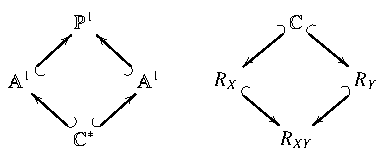
\includegraphics[width=0.78\textwidth]{figures/Fig_044_PDF102_Book090.pdf}
  % [Fig] 原书 p.90
\end{figure}

射影直线上的函数环只有 $\mathbb C$，不能充分反映其几何结构。因此，不能把 $\mathbb P^1$ 上的层看成它的坐标环上的模。解决办法是把 $\mathbb P^1$ 上的相干层视为两条仿射直线上的相干层沿交叠部分粘合而成。具体需要三项数据：有限生成 $R_X$-模 $M_X$、有限生成 $R_Y$-模 $M_Y$，以及它们在交叠处的粘合同构
\[
  \varphi_M\colon M_X\otimes_{R_X}R_{XY}
  \xrightarrow{\ \cong\ }
  M_Y\otimes_{R_Y}R_{XY}.
\]
把这个三元组 $M=(M_X,M_Y,\varphi_M)$ 称为 $\mathbb P^1$ 上的相干层。
% [Tutor Note: 粘合数据的关键在于交叠上 $Y=X^{-1}$，所以 $M_X\otimes_{R_X}R_{XY}$ 只是把 $X$ 局部化：$\mathbb C[X]/(X-\lambda)^n$ 在 $\lambda\ne0$ 时仍非零，而在 $\lambda=0$ 时归零。这正是定理 4.7（射影直线上的相干层分类）中 $S(0,n)$ 只能出现在 $X$ 片、$S(\infty,n)$ 只能出现在 $Y$ 片的原因。写 $\varphi_M$ 时勿忘它同时把 $M_X$ 一侧的 $Y$ 按 $Y=X^{-1}$ 重新解释。]

范畴 $\mathrm{Coh}\,\mathbb P^1$ 中的态射符合预期：它们是成对的模态射
\[
  (\psi_X\colon M_X\to N_X,\quad \psi_Y\colon M_Y\to N_Y),
\]
且须与粘合映射相容。可以把这些态射看作下列复形的零次同调：
\[
  \operatorname{Hom}_{R_X}(M_X,N_X)\oplus
  \operatorname{Hom}_{R_Y}(M_Y,N_Y)
  \xrightarrow{\ d^0\ }
  \operatorname{Hom}_{R_{XY}}(M_{XY},N_{XY}),
\]
其中
\[
  d^0(\psi_X\oplus\psi_Y)
  =\psi_X\otimes_{R_X}R_{XY}
  -\varphi_N^{-1}\circ(\psi_Y\otimes_{R_Y}R_{XY})\circ\varphi_M.
\]

\begin{theorem}{射影直线上的相干层分类}{coherent-sheaves-projective-line}
每个相干层都是下列几类相干层的直和：
\begin{enumerate}[label=(\roman*)]
  \item
  \[
    S(\lambda,n):=
    \left(\frac{\mathbb C[X]}{(X-\lambda)^n},
    \frac{\mathbb C[Y]}{(Y-\lambda^{-1})^n},1\right);
  \]
  \item $S(0,n):=(\mathbb C[X]/(X^n),0,0)$；
  \item $S(\infty,n):=(0,\mathbb C[Y]/(Y^n),0)$；
  \item $\mathcal O(k):=(\mathbb C[X],\mathbb C[Y],Y^k)$。
\end{enumerate}
其中 $\lambda\in\mathbb C^*$、$n\in\mathbb N$、$k\in\mathbb Z$。
\end{theorem}
\begin{proof}[证明思路]
把 $M_X$ 分解为不可分解模的直和。每个分量要么形如 $R_X/(X-\lambda)^n$（$\lambda\in\mathbb C$），要么是自由模 $R_X$。张量上 $R_{XY}$ 后，自由模仍为自由模，而
\[
  R_X/(X-\lambda)^n\quad\text{变为}\quad
  R_{XY}/(X-\lambda)^n.
\]
若 $\lambda\ne0$，后者仍是 $n$ 维的；若 $\lambda=0$，它则变为零。对 $M_Y$ 也可作同样分析，但要注意
\[
  R_{XY}/(Y-\lambda)^n\cong R_{XY}/(X-\lambda^{-1})^n.
\]

配对同构的分量可知，$M_X$ 中每个 $\mathbb C[X]/(X-\lambda)^n$ 都必须与 $M_Y$ 中一个 $\mathbb C[Y]/(Y-\lambda^{-1})^n$ 平衡，每个 $\mathbb C[X]$ 也必须与一个 $\mathbb C[Y]$ 平衡。只有 $M_X$ 中的 $\mathbb C[X]/(X^n)$ 和 $M_Y$ 中的 $\mathbb C[Y]/(Y^n)$ 不必配对，它们可拆出成为不可约相干层 $S(0,n)$ 和 $S(\infty,n)$。

其余部分需要通过同构粘合。例如，若 $M_{XY}=R_{XY}^{\oplus n}$，则粘合自同构是一个元素属于 $R_{XY}$ 的可逆 $n\times n$ 矩阵 $G$。对 $M_X=R_X^{\oplus n}$ 和 $M_Y=R_Y^{\oplus n}$ 施加自同构后，$G$ 只在右乘 $R_X$ 上的可逆矩阵、左乘 $R_Y$ 上的可逆矩阵的意义下确定。Dedekind–Weber 的经典定理说明，可以把 $G$ 化为对角矩阵，对角元是 $Y$ 的整数次幂。因此在这种情形下，该相干层是若干个 $\mathcal O(k)$ 的直和。

另一方面，形如 $R_{XY}/(X-\lambda)^n$ 的 $R_{XY}$-模之间的态射都来自 $R_X$-态射。因此可以假设这些分量之间的粘合映射就是恒等映射，得到若干个 $S(\lambda,n)$ 的直和。更多细节见\bookcite{98}、\bookcite{228}、\bookcite{109}、\bookcite{118}和\bookcite{231}。
\end{proof}

\begin{note}\phantomsection\label{note:projective-line-sheaves}
\textbf{注 4.32.} $S_\lambda:=S(\lambda,1)$ 是点层，而 $\mathcal O(k)$ 是 $\mathbb P^1$ 上的线丛。层 $\mathcal O:=\mathcal O(0)$ 是平凡线丛，也称结构层。
\end{note}

至此，我们构造了通常的相干层范畴，但还希望把它提升为一个 $A_\infty$ 范畴。正如前面用自由分解替代每个模一样，这里也可使用局部自由分解。局部自由层是三元组 $(M_X,M_Y,\varphi_M)$，其中 $M_X,M_Y$ 都是自由模。容易验证，每个相干层都有局部自由分解，可用来构造 dg-Hom 空间。

这里还有一点：如前所见，层之间的态射本身是某个复形的零次同调。因此我们实际上有两个微分；把它们相加，就得到一个大复形。$\mathrm{Coh}^\bullet\mathbb P^1$ 中的态射空间是这些复形的上同调。次数 $0$ 部分是通常的层态射，高次部分则同时度量模之间的代数扩张和粘合过程中的几何障碍。

\begin{example}[线丛之间的 dg-Hom 空间]\label{ex:dg-hom-line-bundles}
$\mathcal O(r)$ 与 $\mathcal O(s)$ 之间的 dg-Hom 空间为
\[
\underbrace{\operatorname{Hom}_{R_X}(R_X,R_X)
\oplus\operatorname{Hom}_{R_Y}(R_Y,R_Y)}_{\text{次数 }0}
\oplus
\underbrace{\operatorname{Hom}_{R_{XY}}(R_{XY},R_{XY})}_{\text{次数 }1},
\]
微分为
\[
  d(f(X)\oplus g(Y))=f(X)-X^{s-r}g(Y).
\]
若 $r>s$，第二项只含 $X$ 的负次幂，因而不可能与第一项抵消，所以零次同调为零。若 $r\leq s$，则零次同调的一组基为
\[
  (f,g)=(X^i,Y^{s-r-i}),\qquad 0\leq i\leq s-r.
\]
于是
\[
  H^0\mathrm{Coh}(\mathcal O(r),\mathcal O(s))=
  \begin{cases}
    \mathbb C(1,Y^{s-r})+\cdots+\mathbb C(X^{s-r},1),&r\leq s,\\
    0,&r>s.
  \end{cases}
\]
另一方面，一次同调是 $\mathbb C[X,X^{-1}]$ 模去由 $X^i$ 和 $X^{s-r-i}$（$i\geq0$）张成的向量空间。若 $s<r-1$，该空间非零，维数为 $r-s-1$：
\[
  H^1\mathrm{Coh}(\mathcal O(r),\mathcal O(s))=
  \begin{cases}
    0,&r\leq s+1,\\
    \mathbb CY+\cdots+\mathbb CY^{r-s-1},&r>s+1.
  \end{cases}
\]
\end{example}

\begin{theorem}{射影直线相干层范畴与克罗内克箭图}{projective-line-kronecker-equivalence}
相干层的导出 $A_\infty$ 范畴 $D\mathrm{Coh}^\bullet\mathbb P^1$ 与 $Q=K_2$（克罗内克箭图）时的 $D\mathrm{mod}^\bullet\mathbb C Q$ 作 $A_\infty$ 等价。
\end{theorem}
\begin{proof}[证明思路]
所有层都可由 $\mathcal O(0)$ 和 $\mathcal O(1)$ 构造：
\begin{itemize}
  \item $\mathcal O(i-1)$ 是映射
  \[
    \mathcal O(i)^{\oplus2}\xrightarrow{\ (1\quad Y)\ }\mathcal O(i+1)
  \]
  的核；
  \item $\mathcal O(i+1)$ 是映射
  \[
    \mathcal O(i-1)\xrightarrow{\binom{1}{Y}}\mathcal O(i)^{\oplus2}
  \]
  的余核；
  \item $S(\lambda/\mu,n)$ 是映射
  \[
    \mathcal O(0)\xrightarrow{\ (\lambda+\mu Y)^n\ }\mathcal O(n)
  \]
  的余核。
\end{itemize}
因此，$D\mathrm{Coh}^\bullet\mathbb P^1=\langle\mathcal O(0),\mathcal O(1)\rangle$。取 $\mathcal O(0)\oplus\mathcal O(1)$，考察它的 $A_\infty$ 自同态代数。由例\ref{ex:dg-hom-line-bundles}的计算可知
\[
  \mathrm{Coh}(\mathcal O(0)\oplus\mathcal O(1),
  \mathcal O(0)\oplus\mathcal O(1))
  =\begin{pmatrix}
    \mathbb C&0\\
    \mathbb C+\mathbb CY&\mathbb C
  \end{pmatrix},
\]
且它集中在次数 $0$。这与克罗内克箭图的路径代数同构，因此
\[
  \langle\mathcal O(0),\mathcal O(1)\rangle
  =D\mathbb C Q=D\mathrm{mod}^\bullet\mathbb C Q.
\]
\end{proof}

\begin{note}\phantomsection\label{note:kronecker-sheaf-identification}
\textbf{注 4.35.} 在上述对应下，奇数长度的弦对象对应线丛 $\mathcal O(k)$；偶数长度的弦对象对应 $S(0,n)$ 和 $S(\infty,n)$；带对象对应 $S(\lambda,n)$。
\end{note}

\begin{proposition}{观察：克罗内克箭图与射影直线上的相干层}{kronecker-quiver-sheaves}
克罗内克箭图的表示论可几何地解释为射影直线上的相干层：
\[
  D\mathrm{Coh}^\bullet\mathbb P^1
  \simeq D\mathrm{Mod}^\bullet K_2.
\]
\end{proposition}

\subsection{线性箭图}\label{subsec:linear-quiver-sheaves}
为了解释线性箭图，需要引入 Landau–Ginzburg 模型\index{landauginzburgmoxing@Landau–Ginzburg 模型|hyperpage}的概念。它由一对 $(X,f)$ 组成，其中 $X$ 是一个空间（仿射簇或轨形），$f\colon X\to\mathbb C$ 是一个函数。可以为这对数据配上带曲率代数 $(R,f)$，其中 $R$ 是 $X$ 的坐标环，而 $f$ 视为 $R$ 中的一个元素。

Landau–Ginzburg 模型 $(X,f)$ 的奇点范畴\index{qidianfanchou@奇点范畴|hyperpage}定义为矩阵分解范畴。我们将在第七章看到，它描述了 $Y=f^{-1}(0)$ 的奇点集的几何。因此也记作
\[
  D\mathrm{Sing}^{\pm}Y=D\mathrm{MF}^{\pm}(R,f).
\]
我们考虑轨形 $X=[\mathbb A^1/G]$ 的情形。前面已看到，它的坐标环应取为代数 $\mathbb C[X]\star G$，该代数同构于循环箭图的路径代数 $\mathbb C Q$。这个代数有中心元 $\ell=X^n$；它在每个投射模 $P_v$ 上的作用，等于乘以从 $v$ 出发并回到 $v$、长度为 $n$ 的路径。该作用给出元素
\[
  \mu_0(1)\in\operatorname{Hom}(P_v,P_v),
\]
可据此把 $P^\bullet$ 的 $\mathbb Z_2$-分次版本变成一个带曲率范畴 $P^\pm_\ell$。$DP^\pm_\ell$ 中的对象是二元组 $(P,d)$，其中 $P$ 是 $\mathbb Z_2$-分次投射 $\mathbb C Q$-模，$d\colon P\to P$ 是次数 $1$ 的映射，且 $d^2$ 的作用等于乘以 $\ell$。

\begin{theorem}{线性箭图奇点范畴中的不可分解对象}{linear-quiver-matrix-factorizations}
$DP^\pm_\ell$ 中每个不可分解对象都是下列形式的扭曲复形：
\[
  M_{ij}:=\left(P_i\oplus P_j[1],
  \begin{pmatrix}0&p_{ij}\\p_{ji}&0\end{pmatrix}\right),
\]
其中 $p_{uv}$ 是从 $v$ 到 $u$ 的最短路径。
\end{theorem}
\begin{proof}[证明思路]
设 $(P,d)$ 是任意矩阵分解。将 $d$ 拆成两个部分 $d_{10}+d_{01}$，分别连接次数 $0$ 部分与次数 $1$ 部分。由于
\[
  \operatorname{Hom}(P_v,P_w)=p_{wv}\mathbb C[\ell],
  \qquad \mathbb C[\ell]\text{ 是主理想整环},
\]
可以分别在 $P^0$ 和 $P^1$ 中选取基，使 $d_{01}$ 化为对角矩阵。关系 $d_{01}d_{10}=\ell$ 又说明 $d_{10}$ 也为对角矩阵。若 $(P,d)$ 不可分解，则 $d_{01}$ 是一个 $1\times1$ 矩阵，故对象必为 $M_{ij}$ 的形式。
\end{proof}

下面简要考察这些对象之间的 Hom 空间：
\[
  \operatorname{Tw}P^\pm_\ell(M_{ij},M_{kl})=
  \begin{pmatrix}
    p_{ki}\mathbb C[\ell]&p_{kj}\mathbb C[\ell]\\
    p_{li}\mathbb C[\ell]&p_{lj}\mathbb C[\ell]
  \end{pmatrix}.
\]
若将该矩阵中的元素记作 $\begin{pmatrix}a&b\\c&d\end{pmatrix}$，其微分为
\[
  d\begin{pmatrix}a&b\\c&d\end{pmatrix}
  =\begin{pmatrix}0&p_{kl}\\p_{lk}&0\end{pmatrix}
   \begin{pmatrix}a&b\\c&d\end{pmatrix}
  -\begin{pmatrix}a&-b\\-c&d\end{pmatrix}
   \begin{pmatrix}0&p_{ij}\\p_{ji}&0\end{pmatrix}.
\]
当 $i=j$ 或 $k=l$ 时，上同调总为零，所以 $M_{ii}$ 是零对象。此外，由于 $M_{ij}=M_{ji}[1]$，可以假设 $i<j$ 且 $k<l$。注意，下标本来是循环的；这里暂且令其依次取 $0,\ldots,n-1$。在这些假设下得到下表，其中
\[
  \iota=\begin{pmatrix}p_{ki}&0\\0&p_{lj}\end{pmatrix},
  \qquad
  \gamma=\begin{pmatrix}0&p_{kj}\\p_{li}&0\end{pmatrix}.
\]

\begin{lemma}{循环箭图矩阵分解的态射}{linear-quiver-matrix-factorization-homs}
\[
\begin{array}{c|c|c}
\text{情形}&DP^0_\ell(M_{ij},M_{kl})&DP^1_\ell(M_{ij},M_{kl})\\\hline
i\leq k<j\leq l&\mathbb C\,\iota&0\\
k<i\leq l<j&0&\mathbb C\,\gamma\\
\text{其他情形}&0&0
\end{array}
\]
\end{lemma}

这与长度为 $n-1$ 的线性箭图的态射表完全相同，只需作如下对应：
\[
  M_{ij}\longleftrightarrow S_{i+1,j}.
\]

\begin{proposition}{观察：线性箭图与 Landau–Ginzburg 奇点范畴}{linear-quiver-landau-ginzburg}
线性箭图的表示论可几何地解释为一个 Landau–Ginzburg 模型的奇点范畴：
\[
  D\mathrm{MF}^{\pm}([\mathbb A^1/\mathbb Z_n],X^n)
  \cong_\infty D\mathrm{Mod}^{\pm}\mathbb C L_{n-1}.
\]
\end{proposition}

\section{范畴图景}\label{sec:picturing-categories}
\takeaway{按相位把不可分解对象排在 $X$ 轴上、并画出不可分解的次数 $0$ 角态射，即得 Auslander--Reiten 箭图；移位表现为滑移反射。几何解释给出对称性：线性情形是旋转 $2\pi/(n+1)$（AR 平移），克罗内克情形是 Dehn 扭转与 $\mathrm{PGL}_2(\mathbb C)$ 作用，循环情形是旋转 $2\pi/n$ 与缩放。}
本节将画出前面研究过的三种箭图所对应的范畴 $D\mathrm{Mod}^\bullet Q$。每种情形下，我们都会画出所有不可分解对象，并按照相位将它们沿 $X$ 轴排列；同时画出不可分解的次数 $0$ 角态射。这里的角态射不能写成更小角态射的乘积。由于角总是正向的，它们都指向 $X$ 轴的正方向。

所得图形也称为 Auslander–Reiten 箭图，在有限维代数的表示论中已有详细研究\bookcite{13}。相干层范畴 $D\mathrm{Coh}^\bullet\mathbb P^1$ 的图示见\bookcite{136}。

对每个范畴，我们还会讨论它的对称性。这些对称性来自几何解释，并可看成相应范畴之间的 $A_\infty$ 函子。不同的几何解释往往会带来不同的对称性。

\subsection{线性箭图}\label{subsec:picturing-linear-quiver}
利用分次线段的解释，下图展示了范畴 $DS^\bullet=DP^\bullet$：
\begin{figure}[H]\centering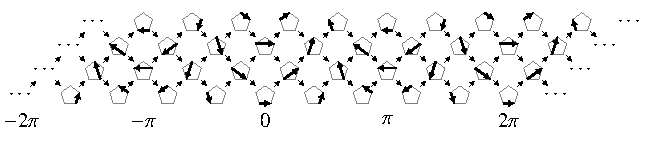
\includegraphics[width=0.96\textwidth]{figures/Fig_045_PDF107_Book095.pdf}
  % [Fig] 原书 p.95
\end{figure}

图中按网格排列对象：横轴是线段的相位，纵轴是线段起点与终点之间的逆时针角差。因此，移位算子是一个滑移反射：它使相位增加 $\pi$，并交换起点与终点；几何上等于先平移 $\pi$，再作一次水平反射。

也可以为线性箭图表示的导出范畴画出同一幅图，并在其中清楚地辨认子范畴 $S^\bullet$、$\mathrm{mod}^\bullet Q$ 和 $P^\bullet$：
\begin{figure}[H]\centering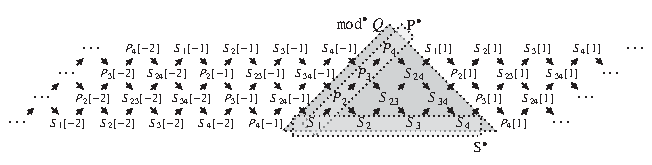
\includegraphics[width=0.96\textwidth]{figures/Fig_046_PDF108_Book096.pdf}
  % [Fig] 原书 p.96
\end{figure}

几何解释还显示，这个范畴有一个特殊的自等价 $R$：它将所有线段旋转
\[
  \frac{2\pi}{n+1}
\]
，同时给所有相位加上同一个角度。从几何角度看，这个自等价显而易见；但若从 $D\mathrm{mod}^\bullet Q$ 的角度看，它就相当深刻。该函子把一些表示映到另一些表示，例如当 $i>2$ 时，$S_i$ 映到 $S_{i-1}$；但 $S_1$ 被映到表示 $P_n[1]$ 的移位。在表示论中，这个函子也称为 Auslander–Reiten 平移\index{auslanderreitenpingyi@Auslander–Reiten 平移|hyperpage}（或按旋转方向不同称其逆函子），在图中对应沿水平方向平移 $\frac{2\pi}{n+1}$。
% [Tutor Note: 旋转 $R$ 在几何侧只是把多边形转过 $2\pi/(n+1)$，但它在表示论侧就是 Auslander--Reiten 平移 $\tau$：这是导出范畴的固有自等价，一般不能由 $\mathrm{mod}\,Q$ 的普通自等价实现。它把 $S_1$ 送到 $P_n[1]$ 而非某个简单模，正说明必须使用导出范畴；这也是图中 $S_1[1]$ 与 $P_n[1]$ 并列出现的原因。]

\begin{note}\phantomsection\label{note:rolled-up-linear-quiver}
\textbf{注 4.39.} 对第二种几何解释，我们只使用了 $\mathbb Z_2$-分次版本。这意味着可以忘掉线段的相位；范畴 $DS^\pm$ 是 $DS^\bullet$ 的 wrapped 版本，其中只含有 $\mathrm{mod}\,Q$ 的两个副本，并将它们粘合成一个圆柱：
\begin{figure}[H]\centering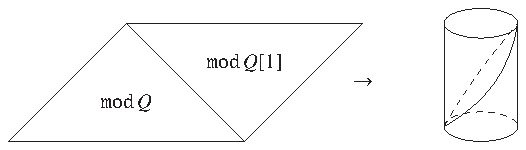
\includegraphics[width=0.78\textwidth]{figures/Fig_047_PDF108_Book096.pdf}
  % [Fig] 原书 p.96
\end{figure}
\end{note}

\subsection{克罗内克箭图}\label{subsec:picturing-kronecker-quiver}
对克罗内克箭图而言，所有相位水平的曲线都形如 $B(-,n)$。若只按相位作为横轴作图，它们都会落在同一点。为区分它们，我们把它们放进一个宽度由 $\lambda$ 参数化、高度由 $n$ 参数化的方框中。这样，在相位为 $\pi$ 的整数倍处得到一列对象。塔中每个对象都通过单射 $B(\lambda,n)\hookrightarrow B(\lambda,n+1)$ 与上方对象相连，并通过投射 $B(\lambda,n)\twoheadrightarrow B(\lambda,n-1)$ 与下方对象相连。不同 $\lambda$ 的带对象之间没有次数 $0$ 态射。

奇数大小的弦对象具有互不相同的相位：
\[
  S(0,2k+1)\text{ 的相位为 }\frac\pi2-\tan^{-1}(k),
  \qquad
  S(1,2k+1)\text{ 的相位为 }-\frac\pi2+\tan^{-1}(k+1).
\]
每个对象都通过两个次数 $0$ 态射与下一个对象相连，这两个态射分别来自左侧和右侧的嵌入。子范畴 $\mathrm{mod}^\bullet Q$ 由相位属于 $(-\frac\pi2,\frac\pi2]$ 的所有对象组成：
\begin{figure}[H]\centering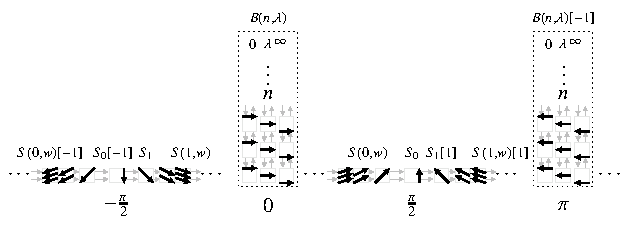
\includegraphics[width=0.96\textwidth]{figures/Fig_048_PDF109_Book097.pdf}
  % [Fig] 原书 p.97
\end{figure}

这幅图显示了范畴的一种对称性：把所有奇数长度的弦对象向右平移 $1$。在圆柱上，这对应于一个 Dehn 扭转：让上边界圆向左转一整圈，就像拧开罐子的盖子。每条穿过圆柱的曲线都因此多出一圈扭转：$S(1,w)$ 变为 $S(1,w+2)$，$S(0,w)$ 变为 $S(0,w-2)$，而 $S_0$ 变为 $S_1[1]$。同样，从曲线角度看这个等价很自然，但从箭图角度看则很不寻常。

第二种对称性来自 $\mathbb P^1$ 上层的几何解释。从这一角度看，每个 $g\in\mathrm{PGL}_2(\mathbb C)$ 都诱导射影直线上的变换，将层 $S(p,n)$ 变为 $S(g\cdot p,n)$。局部自由层在这些变换下不变。这个对称性从 $\mathbb P^1$ 的角度显而易见；但从带标记点的圆柱角度看就很不自然，因为它会混合弦对象与带对象。

\subsection{循环箭图}\label{subsec:picturing-cyclic-quiver}
在这幅图中，除移位外只有两个相位。在 $\frac\pi2$ 处是所有投射模，它们通过箭头 $a_i$ 循环相连；在 $0$ 处是所有有限维模，我们按维数将它们沿竖直方向排列。弦模 $S(i,w)$ 可按起点循环排列。这样便得到一个管状图：每一层高度上，模都通过菱形网格与相邻两层相连。在高度为 $n$ 的倍数处，还会出现一层带对象：
\begin{figure}[H]\centering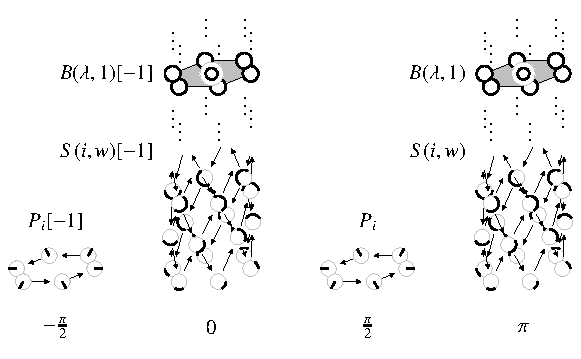
\includegraphics[width=0.94\textwidth]{figures/Fig_049_PDF110_Book098.pdf}
  % [Fig] 原书 p.98
\end{figure}

这里也有对称性。第一种对称性把 $S(i,w)$ 映到 $S(i+1,w)$，把 $P_i$ 映到 $P_{i+1}$，但固定所有 $B(\lambda,k)$。它对应于把带标记点的圆柱旋转 $\frac{2\pi}{n}$。第二种对称性固定所有 $S(i,w)$ 和 $P_i$，但把 $B(\lambda,k)$ 缩放为 $B(r\lambda,k)$；这对应于把轨形 $[\mathbb A^1/G]$ 按比例因子 $r$ 缩放。

\section{同调镜像对称初探}\label{sec:first-glimpse-hms}
\takeaway{箭图表示、$A$ 模型（曲面上曲线的交理论，即 Fukaya 范畴的雏形）与 $B$ 模型（相干层、矩阵分解、奇点范畴）给出同一批 $A_\infty$ 范畴的不同实现；它们本身不必等价，但取导出范畴后等价——这就是同调镜像对称的第一批实例。}
本章中，我们看到某些箭图的表示论可以用两种不同的几何方式来解释。
\begin{itemize}
  \item 第一种解释涉及曲面上曲线的交理论，由此得到一个 $A_\infty$ 范畴：对象是嵌入曲线，态射是交点处（角）的线性组合。这些范畴是更大一类范畴的初步例子，这一类范畴称为 Fukaya 范畴。

  一般来说，Fukaya 范畴描述的是 $2n$ 维辛流形中某些 $n$ 维子流形（称为拉格朗日子流形）的交理论。与曲面上的曲线类似，两个拉格朗日子流形通常会在若干点相交，因此可用交点作为态射空间的一组基。这样的范畴有许多不同版本：Fukaya 范畴、wrapped Fukaya 范畴、Fukaya–Seidel 范畴等。这类构造常称为 A 模型，因为它们与物理学中的 IIA 型超弦理论有关。

  \item 第二种解释涉及复代数簇上的相干层。相干层是向量丛的推广，而态射则度量层之间的映射（次数 $0$）、映射存在的障碍和层之间的扩张（高次）。这类范畴也有许多版本：相干层的导出范畴、矩阵分解范畴、奇点范畴等。这些构造称为 B 模型，因为它们出现在 IIB 型弦理论中。
\end{itemize}

不同模型（箭图、A 模型和 B 模型）给出的 $A_\infty$ 范畴并非完全等价，但取导出范畴后就会等价。这个过程为范畴添加了更多对象，使其在某种意义下更为良好，同时不改变其表示论。

下面列出目前已经建立对应关系的模型。列表看起来不长，但它只是冰山一角。事实上，只要有一些创造性，几乎可以为任何 A 模型找到合适的 B 模型，反之亦然。这一现象由超弦理论预言，如今称为同调镜像对称。下一部分将详细考察这一思想。
\begin{figure}[H]\centering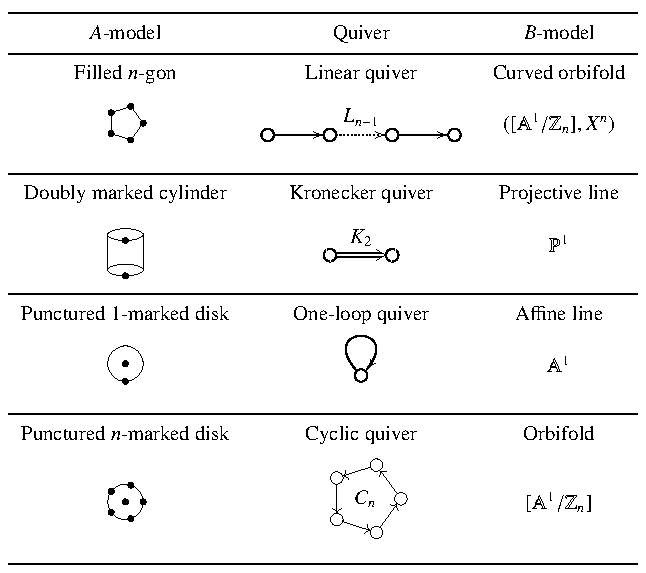
\includegraphics[width=0.92\textwidth]{figures/Fig_050_PDF111_Book099.pdf}
  % [Fig] 原书 p.99
\end{figure}

\section{练习}\label{sec:chapter4-exercises}
\begin{exercise}\label{exer:quiver-orientation-independence}
设 $Q$ 是一个有 $n$ 个顶点、$n-1$ 条箭头的箭图，顶点沿直线排列，但箭头方向不必一致。证明：在等价意义下，$D\mathrm{mod}^\bullet\mathbb C Q$ 不依赖于箭头的定向。（提示：在 $(n+1)$ 边形中选取一些直线，使它们的自同态环为 $\mathbb C Q$。）
\end{exercise}

\begin{exercise}\label{exer:linear-quiver-generators}
设 $Q$ 是有 $n$ 个顶点的线性箭图，且 $X_1,\ldots,X_k\in D\mathrm{mod}^\bullet Q$ 是分别对应于 $(n+1)$ 边形中分次线段 $L_1,\ldots,L_k$ 的对象。证明：$X_1,\ldots,X_k$ 分裂生成 $D\mathrm{mod}^\bullet Q$，当且仅当这些线段的端点覆盖多边形的所有顶点。
\end{exercise}

\begin{exercise}\label{exer:full-strong-exceptional-sequences}
导出范畴 $D\mathcal C^\bullet$ 中的满强例外序列，是一个有序对象列 $X_1,\ldots,X_k$，满足它分裂生成该范畴，并且
\[
  D\mathcal C^d(X_i,X_j)=
  \begin{cases}
    0,&d\ne0\text{ 或 }i>j,\\
    \mathbb C,&i=j,\ d=0.
  \end{cases}
\]
换言之，所有非平凡态射都在次数 $0$，并且只可能从序列中较早的对象指向较后的对象。确定有三个顶点的线性箭图 $Q$ 所对应的 $D\mathrm{mod}^\bullet Q$ 中所有满强例外序列。
\end{exercise}

\begin{exercise}\label{exer:linear-quiver-autoequivalences}
确定有 $n$ 个顶点的线性箭图 $Q$ 所对应的 $D\mathrm{mod}^\bullet Q$ 的自等价群。
\end{exercise}

\begin{exercise}\label{exer:two-one-cylinder-quiver}
考虑一条边界圆上有两个标记点、另一条边界圆上有一个标记点的圆柱。试把该曲面上线段的交理论解释为下图所示箭图的导出范畴，并描述该范畴中的所有不可分解对象。
\begin{figure}[H]\centering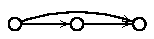
\includegraphics[width=0.48\textwidth]{figures/Fig_051_PDF112_Book100.pdf}
  % [Fig] 原书 p.100
\end{figure}
\end{exercise}

\begin{exercise}\label{exer:spherical-objects-projective-line}
若对象 $X\in D\mathcal C^\bullet$ 的自同态环是 $n$ 维球面的上同调环
\[
  D\mathcal C^\bullet(X,X)\cong\mathbb C\oplus\mathbb C[n],
\]
则称 $X$ 为 $n$-球对象。确定 $D\mathrm{Coh}^\bullet\mathbb P^1$ 中所有 $1$-球对象。
\end{exercise}

\begin{exercise}\label{exer:orbifold-disjoint-disks}
设 $G=\langle g\mid g^{kl}=1\rangle$，并令 $G$ 作用于 $\mathbb C[X]$，满足
\[
  gX=e^{2\pi i/k}X.
\]
证明：$D\mathrm{Coh}^\bullet[\mathbb A^1/G]$ 可用 $l$ 个互不相交、各有一个穿孔且边界上各有 $k$ 个标记点的圆盘的交理论来描述。
\end{exercise}

\begin{exercise}\label{exer:two-punctured-sphere-hms}
证明：有两个穿孔的球面的 A 模型可由 $D\mathbb C[X,X^{-1}]$ 描述，而相应的 B 模型是
\[
  \mathbb A^1\setminus\{0\}=\mathbb P^1\setminus\{0,\infty\}.
\]
因此，A 模型和 B 模型具有相同的底层拓扑空间。
\end{exercise}

\begin{exercise}\label{exer:punctured-orbifold-laurent}
令 $G=\langle g\mid g^n=1\rangle$ 作用于 $\mathbb C[X,X^{-1}]$，满足
\[
  gX=e^{2\pi i/n}X.
\]
证明：$[\mathbb A^1\setminus\{0\}/G]$ 与 $\mathbb A^1\setminus\{0\}$ 的 $B$ 模型等价。
\end{exercise}

\begin{exercise}\label{exer:orbifold-di[已脱敏]}
证明：范畴 $\operatorname{MF}^{\pm}(\mathbb C[X],X^n)$ 可以解释为一个圆盘的 $A$ 模型，其中边界上有一个标记点，圆盘中心有一个 $n$ 阶轨形点。为理解这一点，考虑 $n$ 重覆盖
\[
  \pi\colon D\to D,\qquad z\longmapsto z^n.
\]
$A$ 模型中的对象是覆盖下方的曲线，而乘积则由覆盖空间上方的多边形给出。
\end{exercise}

\chapterreview{%
\textbf{全章地位。}本章是全书第一部完整的词典：同一批不可分解对象，既能写成箭图的表示，又能画成曲面上的曲线，还能读成层。作者用三个可以完全分类的例子把 A 模型与 B 模型并置，同调镜像对称于是在最低维上成为可逐条验证的定理，而不只是物理猜想。

\textbf{知识脉络。}从路径代数 $\mathbb C Q$ 出发，先由基本投射模与基本简单模得到包含关系 $DS^\bullet\subset D\mathrm{mod}^\bullet Q\subset DP^\bullet$；无有向圈时三者等价，有圈时三者分离，这就迫使读者进入导出范畴。随后把三个箭图逐个画出来：线性箭图给出 $(n+1)$ 边形中的分次线段，克罗内克箭图给出圆柱上的弦与带，循环箭图给出带无穷远端的圆柱。再把角读成态射、把锥读成拼接、把多边形读成高阶乘积，交理论模型便与 $A_\infty$ 结构合为一体。最后一节换到代数几何一侧，用 $\mathbb A^1$、$\mathbb P^1$、轨形 $[\mathbb A^1/\mathbb Z_n]$ 上的相干层和 Landau--Ginzburg 模型的奇点范畴重讲同一批例子，两种解释在导出范畴层面重合。

\textbf{核心结论。}（1）$DS^\bullet\subset D\mathrm{mod}^\bullet Q\subset DP^\bullet$，且当 $Q$ 无有向圈时三者都是等价；有圈时 $DS^\bullet$ 只含幂零模，$D\mathrm{mod}^\bullet Q$ 则遗漏顶点位于有向圈上的基本投射模 $P_v$。（2）不可分解对象分类：线性箭图为 $S_{ij}$ 的移位；克罗内克箭图为弦对象 $S(i,w)$ 与带对象 $B(\lambda,n)$，偶长弦对象是 $\lambda\to0,\infty$ 时带对象的极限；循环箭图的 $S(i,w)$、$B(k,\lambda)$、$P_i$ 分别落在 $DS^\bullet$、$D\mathrm{mod}^\bullet Q$、$DP^\bullet$ 中。（3）态射由交点处的角生成，次数为 $(\beta-(\theta_2-\theta_1))/\pi$；锥对应沿角拼接线段，多边形则给出 $\mu(\alpha_1,\ldots,\alpha_{k-1})=\pm\overline\alpha_k$。（4）几何实现：线性箭图的交理论模型给出 $DS^\bullet\cong_\infty\mathrm{Polygon}_{n+1}^\bullet$；克罗内克箭图在导出层面等价于 $\mathbb P^1$ 上的相干层；循环箭图对应轨形相干层，其 Landau--Ginzburg 奇点范畴又给出线性箭图 $L_{n-1}$。

\textbf{辨析与提醒。}其一，三个范畴的记号必须随时区分：同一箭图表示在 $DS^\bullet$ 中表现为 $S_\rho$，在 $D\mathrm{mod}^\bullet Q$ 中表现为模 $M_\rho$，在 $DP^\bullet$ 中表现为扭曲复形 $P_\rho$，三者只在幂零情形才重合。其二，相位与定向是全章最容易出错处：反向线段相位加 $\pi$，移位加 $\pi$，角的次数公式中 $\beta$ 与 $\theta_i$ 必须同向取；只给其中一个量加 $\pi$ 会整体差一次移位。其三，循环箭图 $C_n$ 对应的不是 $L_n$ 而是 $L_{n-1}$，奇点范畴一节的这个下标差一是结构使然，不是笔误。

\textbf{评注。}作者把“导出范畴才是正确栖居地”这一信念放在最前面，而不是先讲高维辛几何，这是全书最有效的教学决定：读者先在能画全的例子里看到等价真正发生，之后遇到泡、Novikov 环与虚拟基本类时，才知道那些技术是为谁服务的。代价同样明显——一切都在曲线上进行，高维才有的现象被完全抹平，读者容易把“箭图就是 Fukaya 范畴”当成一般事实。另一处值得称道的是把弦对象与带对象的极限关系讲透（$B(\lambda,n)$ 在参数边界退化为偶长弦对象），这实际上是后文 partially wrapped 与局部化思想的胚胎。阅读时建议亲手算一遍三种箭图的态射表，再把范畴图景中的旋转看成 Auslander--Reiten 平移，收获会比读定义大得多。}


\part{镜中一瞥}
% 第 5 章：来自物理的动机
\chapter{来自物理的动机}\label{ch:physics-motivation}
本章旨在介绍镜像对称理论背后的物理动机。我们将简要勾勒从经典物理到超弦理论的发展脉络，并说明 A 模型与 B 模型在超弦理论\index{xianlilun@弦理论|hyperpage}中的来源。关于底层物理的更多细节，可参阅讲义\bookcite{62,251}和专著\bookcite{64,114}。

随后，我们将从范畴论的角度考察物理学，重点放在其代数结构上，并暂且假定路径积分形式等技术问题都能够妥善处理。

\section{路径积分形式}
\takeaway{经典物理用最小作用量原理在构型空间寻找临界点；量子理论则以路径积分把配分函数与可观测量的期望值写成对所有路径的求和，作用量以 $e^{iS/\hbar}$ 加权，$\hbar\to0$ 时只有经典解有贡献。}
\subsection{最小作用量原理}
经典物理的许多方面都可以用最小作用\index{zuoyong@作用|hyperpage}量原理来描述：系统状态的演化方式使某个称为作用量的量达到最小。

例如，设一粒子在流形 $M$ 上运动，其运动可由光滑曲线 $\gamma\colon[a,b]\to M$ 描述。记所有此类路径组成的空间为 $X$。作用量可视为一个函数 $S\colon X\to\mathbb R$。若指定粒子的起点与终点 $x_a,x_b\in M$，则粒子所走的路径应当使作用量在
\[
  X(x_a\to x_b)=\{\gamma\in X\mid \gamma(a)=x_a,\ \gamma(b)=x_b\}
\]
上取最小值。

系统中的每个可观测量都可以看成函数 $F\colon X\to\mathbb R$。例如，时刻 $u\in[a,b]$ 的速度是函数 $v_u\colon X\to\mathbb R$，其定义为 $v_u(\gamma)=\frac{d\gamma}{dt}(u)$。借助最小作用量原理求出解之后，只需将解代入可观测量，就能得到它的取值。所有可观测量共同构成一个代数 $\mathcal O$。

\begin{note}\label{note:classical-physics-observation}
\textbf{观察 5.1.} 经典物理的工作，是在构型空间中寻找临界点，并在这些临界点上计算函数（可观测量）的值。
\end{note}

\subsection{量子理论}
量子力学的主要思想是：粒子并不沿着一条预先指定的路径运动，而是所有可能路径都会以一定的振幅对观测结果作出贡献。在量子力学的路径积分形式\index{lujingjifenxingshitixi@路径积分形式体系|hyperpage}中，我们把 $X$ 看作带测度 $(X,[d\gamma])$ 的可测空间，并在其上积分。一般而言，这一步并不简单；这里我们假定这样的测度存在。量子系统的行为由理论的配分函数\index{peifenhanshu@配分函数|hyperpage}和可观测量的期望值决定，它们定义为
\[
  Z=\int_X e^{iS(\gamma)/\hbar}[d\gamma],\qquad
  \langle F\rangle=\int_X F(\gamma)e^{iS(\gamma)/\hbar}[d\gamma],
\]
其中 $S$ 是经典作用量，$\hbar$ 是普朗克常数。
% [Tutor Note: 原文把 $X$ 直接当作可测空间并写出路径积分，这里省略了两点：其一，Feynman 测度 $[d\gamma]$ 一般不存在 $\sigma$-可加版本，需用 Wick 旋转或格点正则化才能严格定义；其二，物理文献通常把期望值归一化为 $\langle F\rangle=Z^{-1}\int F e^{iS/\hbar}[d\gamma]$，原文未除以 $Z$。]

令普朗克常数 $\hbar$ 趋于 $0$，便能看出量子物理与经典物理之间的联系。若 $S(\gamma)$ 变化很大，$e^{iS(\gamma)/\hbar}$ 就会快速振荡，而相应路径对积分的贡献彼此抵消。在极限中，只有满足 $\delta S=0$ 的路径 $\gamma$ 才有贡献；它们正是经典解。

这一形式十分一般，可用于许多不同情形。我们只需给定系统所有可能构型组成的空间 $X$、可观测量代数 $\mathcal O$ 和一种在 $X$ 上积分这些可观测量的表达式的方法。确定这些数据后，便可选取一个作用量 $S\in\mathcal O$，研究系统的动力学。
\begin{itemize}
  \item 可以从时空流形 $M$ 和向量丛 $E\to M$ 出发，令 $X$ 为截面空间 $\Gamma(E)$。这类理论是量子场论\index{liangzichanglun@量子场论|hyperpage}的基本例子。
  \item 也可以从时空流形 $M$ 和主丛 $G\to M$ 出发，令 $X$ 为 $M$ 上所有联络组成的空间，并取联络曲率的总量作为作用量。这就是 Yang--Mills 理论\index{yangmillslilun@Yang–Mills 理论|hyperpage}。
  \item 还可以从 Riemann 曲面 $\Sigma$ 和 Riemann 流形 $X$ 出发，令 $\mathcal X$ 为所有光滑映射 $\sigma\colon\Sigma\to X$ 组成的空间，并取曲面 $\sigma(\Sigma)$ 的面积作为作用量。这可看成弦理论的初步版本：若 $\Sigma$ 是圆柱，映射 $\sigma$ 描述一条闭弦扫过空间 $X$ 的过程。在此设定中，$\Sigma$ 称为世界面，$X$ 称为靶空间。
\end{itemize}

\begin{note}\label{note:quantum-physics-observation}
\textbf{观察 5.2.} 量子物理是在构型空间上、依照一种特殊测度对函数（可观测量）积分。
\end{note}

\section{对称性}
\takeaway{对称性使作用量与测度不变，可观测量应取在不变子空间上；无穷小对称性给出导数 $d_Q$，物理可区分性把可观测量化为 $\ker d_Q/\operatorname{im}d_Q$；超对称则额外引入交换玻色场与费米场的算子。}
\subsection{对称性与上同调}
若有群 $G$ 作用于空间 $X$，且作用量和测度均保持不变，便称物理理论具有对称性；也就是说，对任意 $g\in G$，都有
\[
  S(g\phi)=S(\phi),\qquad [d(g\phi)]=[d\phi].
\]
对称性出现的原因有两种。第一种情形中，$g\phi$ 与 $\phi$ 确实描述系统的不同物理状态。第二种情形中，二者表示同一个物理状态，它们的差异只是来自描述方式的选择。

在后一种情形中，真正的状态空间不是 $X$，而是轨道空间
\[
  X/G=\{G\phi\mid \phi\in X\}.
\]
理论中的可观测量不应依赖描述方式的选择，因此应当在群作用下不变。于是，$X/G$ 上的可观测量就是 $X$ 上的 $G$-不变可观测量。

对称性还有无穷小版本，即每个对称性由一个向量场 $Q\in\Gamma(TX)$ 给出。若 $Q\phi=0$，或等价地 $\exp(tQ)\phi=\phi$，就称 $\phi\in X$ 为不变的。$X$ 上的向量场在函数环上诱导一个导子 $d_Q$：
\[
  d_QF=\lim_{\epsilon\to0}
  \frac{F[\exp(\epsilon Q)\phi]-F[\phi]}{\epsilon}.
\]
若 $d_QF=0$，就称函数 $F$ 在 $Q$ 下不变。理论的可观测量属于 $d_Q$ 的核。形如 $d_QF$ 的可观测量在路径积分中的取值为零：
\begin{align*}
  \langle d_QF\rangle
  &=\int (d_QF)[\phi]e^{iS[\phi]/\hbar}\,d\phi
    =\int d_Q\bigl(Fe^{iS/\hbar}\bigr)[\phi]\,d\phi\\
  &=\lim_{\epsilon\to0}
    \frac{\int Fe^{iS/\hbar}[\exp(\epsilon Q)\phi]\,d\phi-
                \int Fe^{iS/\hbar}[\phi]\,d\phi}{\epsilon}=0.
\end{align*}
最后一行的两个积分相等，因为测度在 $\exp(\epsilon Q)$ 下不变，即 $[d\phi]=[d\exp(\epsilon Q)\phi]$。物理学无法区分相差一个 $d_Q$-像的可观测量。因此，若 $d_Q^2=0$，真正相关的可观测量空间就是
\[
  \frac{\ker d_Q}{\operatorname{im}d_Q},
\]
也就是 $d_Q$ 的上同调。对这一思想作更深入的研究，便会得到 BRST 上同调的概念\bookcite{122}。

\begin{note}\label{note:quantum-symmetry-cohomology}
\textbf{观察 5.3.} 量子物理中的对称性会在可观测量代数上导出上同调理论。
\end{note}

最后，假设作用量可写成 $S=d_QV$，其中 $V$ 是某个可观测量。那么，对任意 $F\in\ker d_Q$，路径积分不依赖于 $\hbar$：
\begin{align*}
  \frac{d}{d\hbar}\langle F\rangle
  &=\frac{d}{d\hbar}\int F e^{i d_QV/\hbar}\,d\phi
   =-\frac{i}{\hbar^2}\int Fd_QV e^{i d_QV/\hbar}\,d\phi\\
  &=-\frac{i}{\hbar^2}\int d_Q(FV)e^{i d_QV/\hbar}\,d\phi
   =-\frac{i}{\hbar^2}\langle d_Q(FV)\rangle=0.
\end{align*}
这意味着我们可以在不改变路径积分的情况下令 $\hbar\to0$，从而把路径积分限制在满足经典方程 $\delta S=0$ 的解空间上。这样量子力学系统就容易处理得多，因此物理学家乐于研究具有这种对称性的理论。
% [Tutor Note: 这是超对称局域化（localization）的原型：$S=d_QV$ 且 $d_QF=0$ 时，$\hbar$ 依赖被全微分吸收。严格化还需：$d_Q$ 在测度上无反常、$V$ 的边界项可忽略、$Q$ 生成紧群作用；否则 $\int d_Q(FV)e^{iS/\hbar}$ 可能留下边界贡献。]

\subsection{超对称性}
引入超对称\index{chaoduichen@超对称|hyperpage}性是产生更多对称性的一种方式。超对称理论中有两类场：玻色场与费米场。前者由彼此可交换的普通变量描述；后者由反交换的 Grassmann 变量描述。

先看一个简单例子：零维理论（见\bookcite[第 1 章]{62}）。空间 $X$ 是从一点到 $\mathbb R$ 的映射空间，因此场构型空间就是带标准测度的 $X=\mathbb R$。设作用量为 $S=\frac12V(x)^2$，其中 $V$ 是函数。作用量在 $V$ 的零点处取极小值，因此这些点就是经典解。为使计算稍简单，我们采用统计力学的约定：去掉因子 $i/\hbar$，并加上负号以使积分收敛。此时配分函数为
\[
  Z=\int_{\mathbb R}e^{-S}\,dx
   =\int_{\mathbb R}e^{-V(x)^2/2}\,dx,
\]
而这个积分通常并不容易计算。

我们可以通过引入两个额外的费米子 $\psi_+,\psi_-$ 来改变该理论。此时可观测量代数变为
\[
  \mathcal O=C^\infty(\mathbb R)\otimes\Lambda^2
  =\frac{C^\infty(\mathbb R)\langle\psi_+,\psi_-\rangle}
  {\langle\psi_+^2,\psi_-^2,\psi_+\psi_-+\psi_-\psi_+\rangle},
\]
并在作用量中加入一项：
\[
  S=\frac12V(x)^2-\psi_+\psi_-\frac{dV(x)}{dx}.
\]
用 Taylor 级数展开作用量的指数，并利用 Grassmann 变量 $\psi_+,\psi_-$ 的平方为零，得到
\[
  \exp(-S)=\left(1+\psi_+\psi_-\frac{dV(x)}{dx}\right)e^{-V(x)^2/2}.
\]
为了计算积分，还需规定如何对 Grassmann 变量积分。正确的规则是 $\int d\psi=0$，$\int\psi\,d\psi=1$。依此对 $\psi_+,\psi_-$ 积分，再利用表达式中的因子 $dV(x)/dx$ 作变量代换 $x\mapsto V$，便得到超对称（SUSY）配分函数
\[
  Z_{\mathrm{SUSY}}=\int_{\mathbb R}\frac{dV(x)}{dx}e^{-V(x)^2/2}\,dx
  =\int_{V(-\infty)}^{V(+\infty)}e^{-V^2/2}\,dV.
\]
若 $V$ 是递增双射，这就是高斯积分，结果为 $\sqrt{2\pi}$；若 $V$ 递减，则多出一个负号。一般地，只要 $V$ 在两端的极限均为无穷，就可以把该积分重新解释为：统计 $V$ 沿正方向穿过零点的次数，再减去沿负方向穿过零点的次数。若结果为 $1$，则 $V$ 总体递增，且 $Z=\sqrt{2\pi}$；若结果为 $-1$，则 $V$ 总体递减，且 $Z=-\sqrt{2\pi}$。也可以写成
\[
  Z_{\mathrm{SUSY}}=\sqrt{2\pi}
  \sum_{V(x)=0}\frac{V'(x)}{|V'(x)|}.
\]
所以，原理论的配分函数可能很复杂，而超对称理论的配分函数只是对经典解作带符号计数。

此外，该理论还有两个交换玻色子与费米子的无穷小对称性：
\[
  Q_+x=\epsilon\psi_+,\quad Q_+\psi_+=0,\quad Q_+\psi_-=\epsilon V(x),
  \qquad
  Q_-x=\epsilon\psi_-,\quad Q_-\psi_-=0,\quad Q_-\psi_+=\epsilon V(x).
\]
这些对称性称为超对称性。因为这里有两个超对称算子，该理论称为 $N=2$ 超对称理论。
% [Tutor Note: 原文的超对称变换印作 $Q_-x=\epsilon\psi_+$，与 $Q_+x=\epsilon\psi_+$ 完全重复，应为 $\psi_-$（译文已改）。另外 Grassmann 积分规则 $\int d\psi=0$、$\int\psi\,d\psi=1$ 即 Berezin 积分，等价于取最高次外形式的系数；这里的 $Z_{\mathrm{SUSY}}$ 是局部化公式的零维原型。]

\begin{note}\label{note:susy-observation}
\textbf{观察 5.4.} 超对称理论是带有一个或多个次数为 $1$、平方为零的算子的 $\mathbb Z_2$-分次理论。为理论加入超对称性能够使计算更易处理。
\end{note}

\section{超弦理论}
\takeaway{把弦的世界面看作二维场论，加入费米场后得到 $d=2,N=(2,2)$ 超对称；在 Kähler 靶空间上，选取不同的超对称子代数分别给出 A 模型（只依赖辛结构，计数全纯映射）与 B 模型（只依赖复结构，局部可观测量为 Dolbeault 上同调）。}
\subsection{从场到弦}
现在把这一思路用于弦理论。固定一个 Riemann 曲面 $\Sigma$ 和靶空间 $X$。映射空间 $\{\sigma\colon\Sigma\to X\}$ 等于平凡 $n$ 维丛的截面空间，因此该理论可视为定义在二维时空 $\Sigma$ 上、含有 $n$ 个标量场的场论。从这一角度看，为使理论具有超对称性而加入额外场是合理的。先考虑 $\Sigma=\mathbb C$ 且 $X=\mathbb R^n$ 的情形。

与零维例子类似，每个标量场都要配上两个费米场。记标量场为 $\phi^I$，费米场为 $\psi_\pm^I$。乍看之下，每个坐标都可以有一族由两个参数控制的超对称性；但 $X$ 上的坐标变换会混合不同坐标对应的场，所以所有场必须共享同一族由两个参数控制的超对称性。这种理论称为 $d=2,N=2$ 理论，其中 $d$ 表示世界面 $\Sigma$ 的维数，$N$ 表示超对称性的数目。

若进一步假设 $X=\mathbb C^n$，还可以得到更多超对称性。此时有两组 $n$ 个标量场：$\phi^i$ 及其共轭 $\phi^{\bar i}$，并有四组费米场 $\psi^i_\pm,\psi^{\bar i}_\pm$。由于坐标变换中实部和虚部相伴变化，我们可以再加入两种超对称性。这种理论称为 $d=2,N=(2,2)$ 理论。在平直空间中，变换为
\[
\begin{aligned}
  \delta\phi^i&=i\alpha_-\psi^i_++i\alpha_+\psi^i_-,&
  \delta\psi^i_\pm&=-\widetilde\alpha_\pm\partial_\pm\phi^i,\\
  \delta\phi^{\bar i}&=i\widetilde\alpha_-\psi^{\bar i}_+
                       +i\widetilde\alpha_+\psi^{\bar i}_-,&
  \delta\psi^{\bar i}_\pm&=-\alpha_\pm\partial_\pm\phi^{\bar i},
\end{aligned}
\]
其中 $\alpha_\pm,\widetilde\alpha_\pm$ 是四个参数，$\partial_+,\partial_-$ 分别表示对复坐标 $z$ 及其共轭坐标的导数。

\begin{note}\label{note:complex-scalar-susy}
\textbf{观察 5.5.} 带有复标量场的量子场论可以赋予 $N=(2,2)$ 超对称性。
\end{note}

到目前为止，我们只把 $X$ 看作复向量空间；但我们希望理论可以取任意带相容度量的复流形作为靶空间。这样的流形称为 Kähler 流形\index{khlerliuxing@Kähler 流形|hyperpage}。它是实维数为 $2n$ 的流形，带有以下三种结构：
\begin{itemize}
  \item Riemann 度量 $g\colon TX\times TX\to\mathbb R$；
  \item 复结构 $J\colon TX\to TX$，满足 $J^2=-1$；
  \item 辛形式 $\omega\in\Omega^2(X)$。
\end{itemize}
三种结构由恒等式 $g(X,JY)=\omega(X,Y)$ 联系起来，知道其中两种即可推出第三种。
% [Tutor Note: 恒等式 $g(X,JY)=\omega(X,Y)$ 的符号依赖 $J$ 与 $\omega$ 的约定：若改用 $g(-,-)=\omega(-,J-)$ 定义度量，则整体符号翻转。Kähler 条件除三者相容外还要求 $d\omega=0$ 且 $J$ 可积，原文此处只列出三种结构。]

利用这些结构，可以把 $\mathbb C^n$ 上的超对称性推广到 $X$：只需利用度量的 Levi--Civita 联络，把导数换成协变导数。为完整起见，下面列出全部超对称变换规则和超对称作用量：
\begin{align*}
  \delta\phi^i&=i\alpha_-\psi^i_++i\alpha_+\psi^i_-,&
  \delta\psi^i_\pm&=-\widetilde\alpha_\pm\partial_\pm\phi^i
    -i\alpha_\pm\psi^k_\mp\Gamma^i_{km}\psi^m_\pm,\\
  \delta\phi^{\bar i}&=i\widetilde\alpha_-\psi^{\bar i}_+
    +i\widetilde\alpha_+\psi^{\bar i}_-,&
  \delta\psi^{\bar i}_\pm&=-\alpha_\pm\partial_\pm\phi^{\bar i}
    -i\widetilde\alpha_\pm\psi^{\bar k}_\mp
       \Gamma^{\bar i}_{\bar k\bar m}\psi^{\bar m}_\pm,
\end{align*}
\begin{align*}
S=\int_\Sigma\bigl(&g_{i\bar j}\,\partial_z\phi^i\partial_{\bar z}\phi^{\bar j}
 +ig_{i\bar j}\psi^i_+D_{\bar z}\psi^{\bar j}_+
 +ig_{i\bar j}\psi^i_-D_z\psi^{\bar j}_-\\
&+g_{\bar i j}\,\partial_z\phi^{\bar i}\partial_{\bar z}\phi^j
 +ig_{\bar i j}\psi^{\bar i}_+D_{\bar z}\psi^j_+
 +ig_{\bar i j}\psi^{\bar i}_-D_z\psi^j_-\\
&+\tfrac12R_{i\bar j k\bar l}
  \psi^i_+\psi^{\bar j}_+\psi^k_-\psi^{\bar l}_-\bigr)\,dz\,d\bar z.
\end{align*}
这里 $\Gamma^i_{km}$ 是度量的 Christoffel 符号，$R_{i\bar j k\bar l}$ 是 Riemann 曲率张量；$D_z,D_{\bar z}$ 是由映射 $\Phi\colon\Sigma\to X$ 的拉回联络所给出的协变导数，而该映射在局部由标量场 $\phi^i$ 描述。

若要从 $\mathbb C$ 推广到任意 $\Sigma$，就必须把费米场视为 $\Sigma$ 上某个丛的截面。由于 $\phi^i$ 是标量，等式 $\delta\phi^i=i\alpha_-\psi^i_++i\alpha_+\psi^i_-$ 表明 $\psi^i_+$ 是平凡丛的截面。另一方面，$\delta\psi^i_+=-\widetilde\alpha_+\partial_+\phi^i+\cdots$ 表明 $\psi^i_+$ 是典范丛的截面，因为它像 $1$-形式那样变换：$d\phi^i=\partial_z\phi^i\,dz$。除非 $\Sigma$ 非常特殊，否则这两种要求无法同时满足，因此 $\widetilde\alpha_+$ 与 $\alpha_-$ 不能同时非零。$\alpha_+$ 与 $\widetilde\alpha_-$ 也一样。为了得到合理的理论，必须令某些参数为零；选择保留哪些参数，便得到不同的超弦理论模型。

\begin{note}\label{note:string-susy-choice}
\textbf{观察 5.6.} 对于定义在任意 Riemann 曲面上的弦理论，必须选择保留哪一部分 $N=(2,2)$ 超对称性。
\end{note}

\subsection{A 模型}
在 A 模型中，令 $\alpha_+=\widetilde\alpha_-=-i$，$\alpha_-=\widetilde\alpha_+=0$，并将相应的超对称算子记为 $Q_A$。此时 $\psi^i_-$ 与 $\psi^{\bar i}_+$ 是 $\Sigma$ 上平凡向量丛的截面，且
\[
  d_{Q_A}\phi^i=\psi^i_-,\qquad d_{Q_A}\phi^{\bar i}=\psi^{\bar i}_+.
\]
注意，$\psi^i_-$ 与 $\psi^{\bar i}_+$ 仍然反交换。因此，若把这些场改写为 $d\phi^i$ 和 $d\phi^{\bar i}$，那么在每个 $x\in\Sigma$ 处，由 $\phi^i,\phi^{\bar i},d\phi^i,d\phi^{\bar i}$ 构成的表达式都可解释为 $X$ 上的微分形式，而 $d_{Q_A}$ 就是外微分。因此，局部可观测量代数可看成 $X$ 的德拉姆上同调。

为了计算路径积分，先仔细考察作用量。它可以改写为
\[
  S=S_0+S_1=\int_\Sigma d_{Q_A}V+\int_\Sigma\Phi^*\omega,
\]
其中 $V=g_{i\bar j}(\psi^i_+\partial_{\bar z}\phi^{\bar j}
 +\psi^{\bar j}_-\partial_z\phi^i)$，而辛形式为 $\omega=i g_{i\bar j}\,dz^i\wedge d\bar z^j$。$S_1$ 是闭 $2$-形式在曲面上的积分，因此只依赖于曲面的同调类 $\beta=[\Phi]\in H_2(X)$。

构型空间 $\mathcal X$ 可看成若干连通分支的不交并，每个分支对应映射 $\Phi\colon\Sigma\to X$ 的像所确定的一个同调类。路径积分是对所有同调类求和，并分别在每个分支上作路径积分。每一项中，都可以把因子 $\exp(\frac{i}{\hbar}S_1(\beta))$ 提到积分号外：
\[
  \langle F\rangle=
  \sum_{\beta\in H_2(X)}e^{\frac{i}{\hbar}S_1(\beta)}
  \int_{\{\Phi\in\mathcal X\mid[\Phi]=\beta\}}
       Fe^{\frac{i}{\hbar}\int_\Sigma d_{Q_A}V}\,d\phi.
\]
这个和式中的路径积分不依赖于 $\hbar$，因为作用量 $S_0=\int_\Sigma d_{Q_A}V$ 是 $d_{Q_A}$-正合的。这意味着我们可以把路径积分限制在作用量经典方程的解上。

经典方程 $\delta S_0=0$ 蕴含 $\partial_{\bar z}\phi^i=\partial_z\phi^{\bar i}=0$，也就是说，$\Phi\colon\Sigma\to X$ 实际上是全纯映射。在最简单的情形中，全纯映射只有有限多个，此时路径积分就是对这些全纯嵌入作加权计数。虽然具体映射 $\Sigma\to X$ 依赖于 $X$ 上的复结构 $J$，但其数目及按 $\omega$ 测得的面积都与 $J$ 无关。
% [Tutor Note: “经典方程蕴含全纯”只对 $Q_A$-闭的场构型成立；真正计数全纯映射时还要取稳定映射紧化并定义虚拟基本类（Gromov--Witten 理论），因为全纯映射可能出现气泡与自同构。原文用“最简单的情形”回避了这些技术点；A 模型不依赖 $J$，是因为 $J$ 只用来写方程，而计数与面积由 $\omega$ 决定。]

\begin{note}\label{note:a-model-symplectic}
\textbf{观察 5.7.} A 模型的配分函数只依赖于作为辛流形的 $(X,\omega)$。
\end{note}

\subsection{B 模型}
在 B 模型中，令 $\widetilde\alpha_+=\widetilde\alpha_-=1$，并把对应的超对称算子记为 $Q_B$。此时带上横线指标的 $\psi$ 是 $\Sigma$ 上平凡丛的截面。作变量代换
\[
  d\phi^i:=g_{i\bar j}(\psi^{\bar j}_+-\psi^{\bar j}_-),
  \qquad d\phi^{\bar i}:=\psi^{\bar i}_++\psi^{\bar i}_-.
\]
局部可观测量的复代数是 $X$ 上微分形式代数的复化 $\Omega_{\mathbb C}(X)$。可以验证
\[
  d_{Q_B}\phi^i=0,\qquad d_{Q_B}\phi^{\bar i}=d\phi^{\bar i},
  \qquad d_{Q_B}d\phi^i=d_{Q_B}d\phi^{\bar i}=0.
\]
这意味着零次可观测量只由 $\phi^i$ 构成，而不含共轭变量 $\phi^{\bar i}$。换言之，这些可观测量恰好是 $X$ 上的全纯函数。进一步研究可知，$(\Omega_{\mathbb C}(X),d_{Q_B})$ 的上同调可以识别为 Dolbeault 上同调\bookcite{66,91}，它是复结构的不变量。

为了计算路径积分，可以把作用量改写为
\[
  S=S_0+S_1=\int_\Sigma d_{Q_B}V+\int_\Sigma Z,
\]
其中 $V=-g_{i\bar j}(\psi^i_+\partial_{\bar z}\phi^{\bar j}
 +\partial_z\phi^{\bar j}\psi^i_-)$，而 $Z$ 是一个较复杂的表达式；它不依赖度量 $g_{i\bar j}$ 或辛形式 $\omega$，只依赖复结构 $J$。

\begin{note}\label{note:b-model-complex}
\textbf{观察 5.8.} B 模型的配分函数只依赖于作为复流形的 $(X,J)$。
\end{note}
% [Tutor Note: B 模型零次可观测量（全纯函数）构成的环，在物理文献中称为手征环（chiral ring），其乘法由全纯算符的 OPE 给出；原文用 Dolbeault 上同调作为局部可观测量代数，正是这一物理图像的数学替身。]

\section{范畴论解释}
路径积分形式只是观察量子力学的一种方式。本节将从另一个角度考察量子力学，研究如何用范畴论的观点来解释它。

\takeaway{把时间演化、场论与弦论都看成函子：粒子对应 $\mathrm{Part}$ 的表示，量子场论是配边范畴到 $\mathrm{Hilb}$ 的幺半函子，二维 TQFT 等价于 Frobenius 代数；开弦由（循环）$A_\infty$ 范畴描述，开弦范畴决定闭弦的共形场论。}

\subsection{物理学作为函子}
在经典物理中，系统状态由相空间中的一点描述；相空间就是系统所有可能状态（位置与动量）组成的空间。相空间具有辛流形 $(X,\omega)$ 的结构。为了给系统引入动力学，需要指定一个 Hamilton 函数 $H\colon X\to\mathbb R$，它确定 $X$ 上的向量场 $X_H$，满足 $\omega(X_H,-)=dH$。系统沿该向量场的流演化：存在单参数自同构族 $\phi_t\colon X\to X$，使得 $\frac{d\phi_t}{dt}=X_H$；若系统在时刻 $a$ 的位置为 $v\in X$，那么 $\phi_t(v)$ 就是时刻 $a+t$ 的状态。

我们把这一思想纳入范畴框架。定义范畴 $\mathrm{Part}$：它只有一个对象 $\bullet$，态射空间为 $\mathrm{Part}(\bullet,\bullet)=\mathbb R$。复合由加法给出，即 $t\circ u=t+u$，单位态射为 $0$。这个简单范畴是粒子时间演化的玩具模型，态射 $t$ 可表示为 $\bullet\xrightarrow{t}\bullet$。

经典动力系统可视为函子 $E\colon\mathrm{Part}\to\mathrm{Symp}$：它把唯一对象 $\bullet$ 指派为系统的相空间，而 $E(t)$ 就是系统演化 $t$ 个时间单位后的流。由于 $\phi_{t+u}=\phi_t\phi_u$，这确实是一个函子。

在量子力学中，粒子在给定时刻的状态由 Hilbert 空间中的向量描述。Hilbert 空间是带 Hermitian 内积的复向量空间，而系统的时间演化由酉算子描述。同样，这可以看成函子 $Q\colon\mathrm{Part}\to\mathrm{Hilb}$，也就是范畴 $\mathrm{Part}$ 的一种特殊表示。

\begin{example}[粒子范畴的表示]
为了构造描述粒子在流形 $X$ 上运动的表示，令 $Q(\bullet)=L^2(X,\mathbb C)$，即 $X$ 上平方可积复值函数组成的空间，其内积为
\[
  \langle f,g\rangle=\int_X f\overline g\,dx.
\]
线性映射 $Q(t)$ 可由卷积描述：
\[
  Q(t)f(y)=\int_X G_t(x,y)f(x)\,dx.
\]
卷积因子 $G_t(x,y)$ 是所有满足 $\gamma(0)=x$、$\gamma(t)=y$ 的路径的权重。在路径积分形式中，它可理解为
\[
  G_t(x,y)=
  \frac{\displaystyle\int_{X(x,y)}e^{iS(\gamma)/\hbar}[d\gamma]}
       {\displaystyle\int_Xe^{iS(\gamma)/\hbar}[d\gamma]},
  \qquad
  X(x,y)=\{\gamma\in X\mid\gamma(0)=x,\ \gamma(t)=y\}.
\]
\end{example}

\begin{note}\label{note:ordinary-quantum-representation}
\textbf{观察 5.10.} 普通量子力学可以看成范畴 $\mathrm{Part}$ 的一个表示。
\end{note}

\subsection{拓扑量子场论}
若想把场纳入这一图景，还需要多做一些工作。从数学角度看，场是流形 $M$ 上某个向量丛 $E$ 的截面。与粒子情形中把时间单独处理不同，现在把时间也纳入底流形 $M$，并让 $M$ 充当时空。

动力学仍由某个最小作用量原理支配。所有可能场构型组成的空间是截面空间 $\mathcal F=\Gamma(E)$，作用量则是函数 $S\colon\mathcal F\to\mathbb R$。使作用量达到极小值的场就是经典解。为了选出一个解，可以在 $M$ 的一个余维 $1$ 子空间附近指定场，并试着把它传播到整个 $M$。

如同粒子情形，我们可以尝试用路径积分形式将理论量子化。设 $U\subset M$ 是一块区域，边界分成流入边界 $B_i$ 和流出边界 $B_o$。每个边界都对应一个 Hilbert 空间 $Q(B_{i/o})$，其基由场在该边界上的所有可能状态构成。由此可以构造线性映射 $Q(U)\colon Q(B_i)\to Q(B_o)$；两个状态之间的矩阵系数，是对所有具有相应边界条件的场构型求和，并以依赖作用量的因子加权：
\[
  \langle\phi_o,Q(U)\phi_i\rangle=
  \frac{\displaystyle\int_{\mathcal F(\phi_i,\phi_o)}
       e^{\frac{i}{\hbar}S(\phi)}[d\phi]}
       {\displaystyle\int_{\mathcal F}e^{\frac{i}{\hbar}S(\phi)}[d\phi]},
  \qquad
  \mathcal F(\phi_i,\phi_o)=
  \{\phi\in\mathcal F\mid\phi|_{B_{i/o}}=\phi_{i/o}\}.
\]

现在设有两块区域 $U,V\subset M$，且 $B_{o,U}=B_{i,V}$。沿共同边界粘合后得到区域 $U\cup V$，其流入边界为 $B_{i,U}$，流出边界为 $B_{o,V}$。若作用量可加，即
$S^{U\cup V}(\phi)=S^U(\phi|_U)+S^V(\phi|_V)$，便可证明
$Q(U\cup V)=Q(V)\circ Q(U)$。因此，$Q$ 可以看成某个适当范畴的表示。
% [Tutor Note: 原文此处把矩阵系数印作 $\langle\phi_i,Q(t)\phi_o\rangle$、把复合印作 $Q(U)\circ Q(V)$；按 $Q(U)\colon Q(B_i)\to Q(B_o)$ 的方向，应分别为 $\langle\phi_o,Q(U)\phi_i\rangle$ 与 $Q(V)\circ Q(U)$（译文已改）。此外“作用量可加”还隐含要求沿粘合边界的场迹相容，即拼接处没有跳跃。]
\begin{figure}[H]
  \centering
  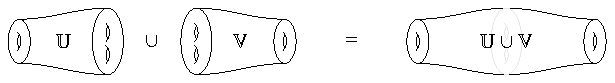
\includegraphics[width=0.62\textwidth]{figures/Fig_052_PDF127_Book115.pdf}
  \caption{沿共同边界粘合两个区域（原书 p.115）}
  \label{fig:cobordism-gluing}
\end{figure}

配边范畴\index{peibianfanchou@配边范畴|hyperpage} $\mathrm{Cob}_n$ 的对象是定向的 $(n-1)$ 维流形，态射是带边界的定向 $n$ 维流形。态射 $U$ 的边界分成两个不交部分 $B_i$ 与 $B_o$：后者继承 $U$ 的定向，前者取相反定向。这样，$U$ 就被视为从 $B_i$ 到 $B_o$ 的态射。两个态射通过公共边界粘合而复合。

根据流形带有的结构（拓扑、光滑、Riemann 度量等），配边范畴有不同版本。量子场论可以看成从适当配边范畴到 Hilbert 空间范畴的函子，并满足一些附加性质。最重要的附加条件是函子必须是幺半的：它把边界分量的不交并映到向量空间的张量积。若配边范畴是拓扑范畴，我们就称之为拓扑量子场论（TQFT）。更多信息可参见\bookcite{246,18}。

\begin{note}\label{note:qft-cobordism}
\textbf{观察 5.11.} 量子场论研究配边范畴的幺半表示。
\end{note}

\subsection{闭弦}
这一观点也适用于弦理论。闭弦是嵌入靶流形中的圆 $\sigma\colon S^1\to X$。弦随时间运动时，会在 $X$ 中扫出一个圆柱。弦还可能出现更复杂的行为，例如产生或消失，或者两条弦融合。这些动力学可以对应到如下配边：
\begin{figure}[H]
  \centering
  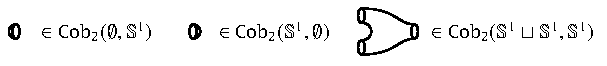
\includegraphics[width=0.74\textwidth]{figures/Fig_053_PDF128_Book116.pdf}
  \caption{闭弦的产生、湮灭与融合（原书 p.116）}
  \label{fig:closed-string-cobordisms}
\end{figure}

为了构造弦的量子理论，我们给每组弦指派一个 Hilbert 空间，并让世界面作为这些空间之间的线性映射；映射系数由适当的作用量原理给出。这自然可以看成二维配边范畴的幺半表示。拓扑弦理论给出从 $\mathrm{Cob}_2$ 到 $\mathrm{Hilb}$（或 $\mathrm{Vect}(k)$）的函子。由于每个拓扑曲面都可以由裤子曲面、圆帽和圆杯拼成，该函子由 $V=F(S^1)$ 和上述三种操作的像决定：单位映射 $k\to V$、迹映射 $V\to k$ 和乘法 $V\otimes V\to V$。这三项数据使 $V$ 成为一个 Frobenius 代数\index{frobeniusdaishu@Frobenius 代数|hyperpage}\bookcite{8}。

\begin{note}\label{note:tqft-frobenius}
\textbf{观察 5.12.} 二维 TQFT 与 Frobenius 代数一一对应。
\end{note}

大多数弦理论并非拓扑理论，而是共形理论，也就是说还必须考虑世界面的复结构\bookcite{215}。相应的共形配边范畴 $\mathrm{CFT}$ 对每个圆的 $n$ 元组有一个对象 $n$；$\mathrm{CFT}(n,m)$ 是带有 $n+m$ 个边界分量的 Riemann 曲面的模空间，并附有与各边界的 $S^1$ 的识别（标架）。该空间按曲面亏格分解为不交并：
\[
  \mathrm{CFT}(n,m):=\coprod_g\mathcal N_{g,n+m}.
\]
给定一个弦理论后，可以尝试计算相应函子 $\mathrm{CFT}\to\mathrm{Hilb}$。此函子把对象 $n$ 映到 Hilbert 空间 $H^{\otimes n}$，其中 $H$ 描述单条弦的所有状态。若在 $\mathrm{CFT}(n,m)$ 中固定一个点（即固定一个曲面 $\Sigma$），路径积分形式会给出映射 $H^{\otimes n}\to H^{\otimes m}$，它由对曲面 $\Sigma$ 上所有可能场构型积分得到。

不仅如此，我们还可以把积分扩展到 $\mathrm{CFT}(n,m)$ 的某个子空间中的所有曲面构型，而不只取一个点。这样，奇异链复形中的每条链都会给出一个映射 $H^{\otimes n}\to H^{\otimes m}$。为使这一想法精确化，定义范畴 $\mathrm{HCFT}^\bullet$：其对象为 $n\in\mathbb N$，而 $\mathrm{HCFT}^\bullet(n,m)$ 是适当的复形，用于计算 $\mathrm{CFT}(n,m)$ 的同调。从这一角度看，路径积分形式可解释为幺半 dg-函子
$F\colon\mathrm{HCFT}^\bullet\to\mathrm{dgVect}^\bullet$。这称为拓扑共形场论\index{tuopugongxingchanglun@拓扑共形场论|hyperpage}\bookcite{90,58,214}。

\begin{example}[A 模型与 Gromov--Witten 不变量]
在 A 模型中，这一思想与 Gromov--Witten 不变量\index{gromovwittenbubianliang@Gromov–Witten 不变量|hyperpage}\bookcite{85}密切相关。设 $X$ 是光滑射影簇，固定 $n,g\in\mathbb N$ 和一个 $2$-循环 $\beta\in H_2(X,\mathbb Z)$。给定 $n$ 个上同调类 $\psi_1,\ldots,\psi_n\in H^\bullet(X,\mathbb Q)$，可以定义 Gromov--Witten 不变量
\[
  GW^X_{\beta,g,n}(\psi_1,\ldots,\psi_n)
  \in H^\bullet(\mathcal M_{g,n},\mathbb Q).
\]
它是 $\mathcal M_{g,n}$ 上的上同调环元素；$\mathcal M_{g,n}$ 是亏格为 $g$、带有 $n$ 个标记点的 Riemann 曲面模空间的紧化（此处是标记点而非边界圆，因此没有标架）。直观上，这些不变量应当计数这样的全纯映射 $\sigma\colon\Sigma\to X$：曲面 $\Sigma$ 的亏格为 $g$，有 $n$ 个标记点，$\sigma(\Sigma)$ 的同调类为 $\beta$，且这些标记点落在与 $\psi_i$ 对偶的同调类上。

下面简述如何把这些数据转化为 $\mathrm{HCFT}^\bullet$ 的表示。取 $H_2(X,\mathbb Z)$ 的一组基 $\beta_1,\ldots,\beta_k$，并令 $K=\mathbb C((t_1,\ldots,t_k))$。若 $\beta=b_1\beta_1+\cdots+b_k\beta_k$，则置 $t^\beta=t_1^{b_1}\cdots t_k^{b_k}$。考察向量空间 $V=H^\bullet(X,K)$。因为 $X$ 光滑且紧致，$V$ 带有双线性配对 $\langle-,-\rangle\colon V\times V\to K$，由此可将 $V$ 与其 $K$-对偶空间识别，并将任意线性映射 $f\colon V^{\otimes_K n}\to V^{\otimes_K m}$ 看作映射 $f\colon V^{\otimes_K(n+m)}\to K$。

固定这些约定后，可以把 Gromov--Witten 不变量转化为 $\mathrm{HCFT}^\bullet$ 的表示。令 $GW^X(n)=V^{\otimes_K n}$；对任意 $\eta\in\mathrm{HCFT}^\bullet(n,m)$，令 $GW^X(\eta)$ 对应于映射
\[
  V^{\otimes_K(n+m)}\to K:\quad
  \psi_1\otimes\cdots\otimes\psi_{n+m}\longmapsto
  \sum_\beta t^\beta\int_\eta
  GW^X_{\beta,g,n+m}(\psi_1,\ldots,\psi_{n+m}).
\]
换言之，映射的系数是对循环 $\eta$ 积分后、再加权求和得到的 Gromov--Witten 不变量，并把 $\eta$ 重新解释为 $\mathcal M_{g,n+m}$ 中的循环。更多细节可参见\bookcite{58}。反过来，从拓扑共形场论出发，也可以计算出某些类似 Gromov--Witten 不变量的数值不变量\bookcite{61,50}。
\end{example}

\begin{note}\label{note:closed-strings-cft}
\textbf{观察 5.14.} 闭弦理论给出 $\mathrm{CFT}$ 或 $\mathrm{HCFT}^\bullet$ 的表示。
\end{note}

\subsection{开弦}
闭弦是嵌入时空的圆，但我们也可以考虑开弦，即嵌入的线段。为了描述开弦的动力学，还必须研究其端点处发生的事情。一般而言，端点被限制在靶空间 $X$ 的某些子流形上，而端点处的场取值在这些子流形上的某些丛中。

这些带有丛的子流形应被视为自身也具有动力学的对象。在物理学中，它们称为膜\index{mo@膜|hyperpage}（brane）；依弦理论模型不同，膜有不同类型。与闭弦理论一样，可以把它们纳入范畴形式体系\bookcite{16}：
\begin{itemize}
  \item 膜是范畴的对象；
  \item 膜之间的交点给出它们之间的态射；
  \item 乘法由弦在这些交点之间运动的方式决定。
\end{itemize}
对固定靶空间 $(X,J,\omega)$，我们得到两个由膜构成的 $A_\infty$ 范畴，一个对应 A 模型，一个对应 B 模型。
\begin{itemize}
  \item A 模型使用辛几何，膜是拉格朗日子流形。它们是满足 $\omega|_{TL}=0$ 的极大子流形 $L\subset X$。对应范畴称为 Fukaya 范畴，其数学定义将在第六章给出。
  \item B 模型中的子流形是复子流形。进一步考虑可知，还必须允许在这些子流形上带有某些丛。这便引出相干层导出范畴的概念，其数学定义将在第七章给出。
\end{itemize}

这些膜范畴与前面讨论的共形场论有何关系？从物理角度看，把开弦接在一起形成闭弦是很自然的，因此原则上可以由开弦版本构造闭弦理论。Costello 在文献\bookcite{58}中证明了这一点。对每个对象集 $\Lambda$，他构造了三个 dg-范畴：$\mathcal O^\bullet_\Lambda$ 描述端点落在 $\Lambda$ 中对象上的开弦；混合版本 $\mathcal{OC}^\bullet_\Lambda$ 同时包含开弦和闭弦；子范畴 $\mathcal C^\bullet$ 则只描述闭弦。最后一个范畴与 $\mathrm{HCFT}^\bullet$ 拟等价，且不依赖 $\Lambda$。它们之间的关系为
\[
  \mathcal O^\bullet_\Lambda\subset
  \mathcal{OC}^\bullet_\Lambda\supset\mathcal C^\bullet.
\]
若有 $\mathcal O^\bullet_\Lambda$ 的一个表示，就可以将其延拓为 $\mathcal{OC}^\bullet_\Lambda$ 的表示，再限制为 $\mathcal C^\bullet$ 的表示。后者可解释为一个上同调共形场论。Costello 还证明，给出 $\mathcal O^\bullet_\Lambda$ 的一个表示，等价于构造一个以 $\Lambda$ 为对象集的（循环）$A_\infty$ 范畴。此外还可证明，导出等价的 $A_\infty$ 范畴会给出等价的 $\mathcal C^\bullet$ 表示。

\begin{note}\label{note:open-string-ainfty}
\textbf{观察 5.15.} 开弦理论由（循环）$A_\infty$ 范畴决定，而导出等价的 $A_\infty$ 范畴给出等价的闭弦理论。
\end{note}

\section{何谓镜像对称？}
在 20 世纪 80 年代和 90 年代，物理学家注意到：某个 Kähler 流形 $X$ 上 A 模型的一些计算，与另一个流形 $X^\vee$ 上 B 模型的计算相吻合。因此他们猜想，每个 A 模型都应当有一个定义在另一流形上的 B 模型，使二者在物理上等价。这一新现象称为镜像对称，而一对流形 $(X,X^\vee)$ 称为镜像对。这个名称源自一种数值不变量：镜像对的 Hodge 菱形\index{hodgelingxing@Hodge 菱形|hyperpage}互为镜像。下图展示五次三维簇及其镜像的 Hodge 菱形：

\takeaway{镜像对称最初表现为一对流形 $(X,X^\vee)$ 上 A/B 模型计算相符、Hodge 菱形互为镜像；Kontsevich 把它提升为同调镜像对称：$D^\pi\mathrm{Fuk}(X)\cong D^\pi\mathrm{Coh}(X^\vee)$ 的 $A_\infty$ 拟等价，其数值不变量对应 Gromov--Witten 不变量与周期。}
\begin{figure}[H]
  \centering
  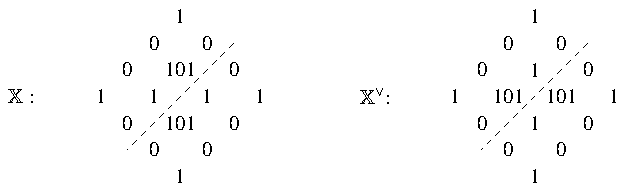
\includegraphics[width=0.88\textwidth]{figures/Fig_054_PDF131_Book119.pdf}
  \caption{五次三维簇及其镜像的 Hodge 菱形（原书 p.119）}
  \label{fig:quintic-hodge-diamonds}
\end{figure}

从数学角度看，这意味着辛几何中的某些问题可以通过在另一流形上做复几何来回答，反之亦然。起初，大多数数学家觉得这个想法近乎荒谬；但当物理学家 Candelas、de la Ossa、Green 和 Parkes\bookcite{51}用它来计数五次三维簇上的曲线时，数学家开始重视它。这些数目可以用 Gromov--Witten 不变量严格定义，但一直很难确定\bookcite{75}；借助镜像对称，Candelas 等人把它们联系到镜像流形上的某些积分（称为周期），并求得它们的生成级数。

人们提出了许多形式化镜像对称的方法。起初，这些表述都采用经典几何框架，使用微分几何、辛几何、复几何和枚举几何中的标准工具\bookcite{92,158}。1994 年，Kontsevich\bookcite{141}提出从范畴论角度考察镜像对称，由此引出了同调镜像对称\index{tongdiaojingxiangduichen@同调镜像对称|hyperpage}的思想。

其核心思想是：镜像对称应当体现为两个 $A_\infty$ 范畴之间的导出等价。一个范畴对应 A 模型，称为 Fukaya 范畴；另一个对应 B 模型，是相干层的导出范畴。其理由是，既然超弦理论可以看成某个 $A_\infty$ 范畴的表示，那么导出等价的 $A_\infty$ 范畴就会给出相同的物理学。数学上，范畴等价又意味着这些范畴的某些数值不变量相同；将这些不变量分别放回辛几何和代数几何的背景中，便可恢复较经典的镜像对称陈述：
% [Tutor Note: 这里 $D^\pi$ 表示分裂导出范畴；同调镜像对称断言的是 $A_\infty$ 拟等价，而不只是三角等价。物理上“导出等价给出相同物理”依赖开闭弦对应：开弦范畴决定闭弦理论（Costello 定理）；数学上还需为 $\mathrm{Coh}(X^\vee)$ 选好增强三角结构，才能谈论 $A_\infty$ 范畴。]
\begin{figure}[H]
  \centering
  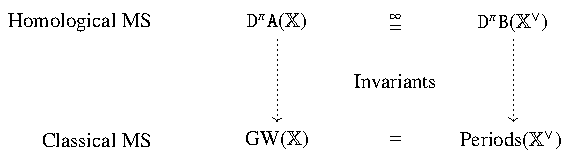
\includegraphics[width=0.68\textwidth]{figures/Fig_055_PDF132_Book120.pdf}
  \caption{同调镜像对称与经典镜像对称之间的关系（原书 p.120）}
  \label{fig:hms-classical-mirror}
\end{figure}

最初，镜像对称只针对一类特殊的 Kähler 流形——紧致 Calabi--Yau 流形提出。后来人们逐渐认识到，这一原理还可推广到其他几何背景：相关空间可以不是 Calabi--Yau\bookcite{5,139,49}，可以非紧\bookcite{1}、非光滑\bookcite{199}，甚至可以非交换\bookcite{11}。为了处理这些新空间，人们构造了 A 模型和 B 模型的若干推广。

接下来的两章将讨论这些 $A_\infty$ 范畴的构造。我们先研究 A 模型及 Fukaya 范畴的不同版本；对 B 模型，我们将定义相干层导出范畴这一 $A_\infty$ 范畴，并考察矩阵分解范畴。本部分最后一章将给出 A 模型与 B 模型等价的若干例子，以展示同调镜像对称这一现象。我们还将讨论如何借助环面几何和热带几何的思想寻找镜像对 $(X,X^\vee)$，并简要勾勒这与该领域两条重要研究方向——SYZ 猜想\bookcite{237}和 Gross--Siebert 纲领\bookcite{104,105}——之间的联系。

\section{练习}
\begin{exercise}\label{exer:physics-free-particle}
令 $M=\mathbb R^2$，并设 $\gamma\colon[0,1]\to M$ 是一条路径。自由运动粒子的经典作用量为 $S(\gamma)=\int_0^1\dot\gamma^2(t)\,dt$。证明：在 $X(x_0\to x_1)$ 中使作用量取极小值的曲线 $\gamma$，以恒定速度沿从 $x_0$ 到 $x_1$ 的直线运动。
\end{exercise}

\begin{exercise}\label{exer:discrete-path-integral}
令 $M=\mathbb R^2$，并令 $I_3=\{0,\frac12,1\}$。离散路径空间为
\[
  X_3(x_0\to x_1):=\{\gamma\colon I_3\to M\mid
  \gamma(0)=x_0,\ \gamma(1)=x_1\}=M,
\]
其上的作用量为
\[
  S(\gamma)=r\left((x_1-\gamma(\tfrac12))^2+
                     (\gamma(\tfrac12)-x_0)^2\right),
\]
其中 $r$ 为常数。证明：路径积分中 $\gamma(\frac12)$ 的期望值为 $(x_0+x_1)/2$。可以假设 $r\in\mathbb C$ 的选取使相关积分收敛。
\end{exercise}

\begin{exercise}\label{exer:loop-rotation-observable}
令 $M=\mathbb C$，并考察闭曲线空间
\[
  X=\{\gamma\colon[0,1]\to M\mid\gamma(0)=\gamma(1)\}.
\]
对与曲线起点旋转对应的向量场 $Q$，都有一参数对称性
\[
  \exp(\epsilon Q)(\gamma)(t)=\gamma(t+\epsilon\bmod1),
\]
它对应于改变曲线的起点。令可观测量 $X_u:=\gamma(u)$，即把曲线 $\gamma$ 映到其在时刻 $u$ 的位置。求 $d_QX_u$。
\end{exercise}

\begin{exercise}\label{exer:lie-algebra-cohomology}
设 Lie 代数 $\mathfrak g=\mathbb Rg_1+\cdots+\mathbb Rg_k$ 作用于空间 $X$。考虑张量积
\[
  K^\bullet:=C^\infty(X)\otimes\Lambda^\bullet(\mathfrak g)
  =C^\infty(X)\otimes
  \frac{\mathbb C\langle g_1,\ldots,g_k\rangle}
  {\langle g_ig_j+g_jg_i\mid1\le i,j\le k\rangle},
\]
并定义微分
\[
  d(\phi g_{i_1}\cdots g_{i_r})=
  \sum_j(g_j\cdot\phi)\,g_j\wedge g_{i_1}\wedge\cdots\wedge g_{i_r}.
\]
证明这是一个复形，并且
\[
  H^0(K)=\{f\in C^\infty(X)\mid
     \forall g\in\mathfrak g,\ g\cdot f=0\}.
\]
再证明：若 $\mathfrak g$ 在 $X$ 上的作用是自由的（即每一点处与 $g_i$ 对应的向量场线性无关），则 $H^1(K)=0$；事实上，所有更高次上同调也都为零。
\end{exercise}

\begin{exercise}\label{exer:susy-invariant-action}
证明作用量
\[
  S=\frac12V(x)^2-\psi_+\psi_-\frac{d}{dx}V(x)
\]
在超对称变换 $Q_\pm$ 下确实不变。
\end{exercise}

\begin{exercise}\label{exer:susy-auxiliary-field}
考虑一个包含两个玻色场 $x,H$ 和两个费米场 $\psi_+,\psi_-$ 的系统。证明作用量
\[
  S=\frac12H^2+iHV(x)-\psi_+\psi_-\frac{d}{dx}V(x)
\]
具有如下超对称性：
\[
  \delta x=\psi_++\psi_-,\qquad
  \delta\psi_\pm=\pm iH,\qquad \delta H=0,
\]
并证明 $\delta^2=0$，且存在表达式 $F$ 使 $S=\delta F$。
\end{exercise}

\begin{exercise}\label{exer:oriented-riemann-kaehler}
证明：每个二维可定向 Riemann 流形都可以看成 Kähler 流形，其中复结构 $J$ 对应于逆时针旋转 $90^\circ$。
\end{exercise}

\begin{exercise}\label{exer:cobordism-one-category}
拓扑配边范畴 $\mathrm{Cob}_1$ 的对象是带符号点集，即每个点都附有 $+$ 或 $-$ 号的有限点集。态射由若干条定向开曲线构成：曲线从 $S_1$ 的正点或 $S_2$ 的负点出发，到达 $S_2$ 的正点或 $S_1$ 的负点；此外还可带有若干条闭曲线。若两个态射之间存在保持端点的同胚，就认为它们相同。
\begin{enumerate}[label=(\roman*)]
  \item 令 $S=\varnothing$。证明 $\mathrm{Cob}_1(S,S)$ 在复合运算下同构于 $(\mathbb N,+)$。
  \item 令 $S=\{p_1^+,\ldots,p_k^+\}$。证明 $\mathrm{Cob}_1(S,S)$ 在复合运算下同构于 $\mathbb N\times S_k$。
  \item 令 $S=\{p^+,q^-\}$。描述半群 $\mathrm{Cob}_1(S,S)$。
\end{enumerate}
\end{exercise}

\begin{exercise}\label{exer:monoidal-cobordism-functor}
函子 $F\colon\mathrm{Cob}_1\to\mathrm{vect}(k)$ 称为幺半函子，若它把带点集的不交并自然地映为张量积：
\[
  F(S_1\sqcup S_2)\cong F(S_1)\otimes F(S_2).
\]
类似地，它也把曲线的不交并映为映射的张量积。精确定义见\bookcite{246}。
\begin{enumerate}[label=(\roman*)]
  \item 证明 $F$ 由下列两个基本配边的像决定：
  \begin{figure}[H]
    \centering
    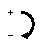
\includegraphics[width=0.15\textwidth]{figures/Fig_056_PDF134_Book122.pdf}\qquad
    
\includegraphics[width=0.15\textwidth]{figures/Fig_057_PDF134_Book122.pdf}
    \caption{一维配边范畴的基本生成态射（原书 p.122）}
    \label{fig:cobordism-one-generators}
  \end{figure}
  \item 证明下图的像给出 $V_+:=F(+)$ 与 $V_-:=F(-)$ 之间的非退化配对。由此推出：每个维数 $n\in\mathbb N$ 恰好对应一个一维 TQFT。
  \begin{figure}[H]
    \centering
    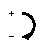
\includegraphics[width=0.18\textwidth]{figures/Fig_058_PDF135_Book123.pdf}
    \caption{诱导配对的配边（原书 p.123）}
    \label{fig:cobordism-pairing}
  \end{figure}
  \item 在无定向配边范畴中，对象只是点集，态射是这些点之间的无定向曲线。描述该范畴及其幺半表示。
\end{enumerate}
\end{exercise}

\begin{exercise}\label{exer:two-dimensional-tqft-frobenius}
设 $F$ 是一个二维 TQFT。证明：相应 Frobenius 代数中的乘法是结合且交换的。此外，证明配对 $(a,b)\mapsto\operatorname{Tr}(a\cdot b)$ 非退化。
\end{exercise}

\chapterreview{%
\textbf{全章地位。}这是全书唯一的物理章，任务不是证明而是建词典：把路径积分、对称性、超对称、超弦这些物理语言逐条翻译成上同调与范畴。第 4 章已在例子里见到 A/B 二重性，第 6、7 章要给出严格构造，本章负责说明这些构造为何值得做。

\textbf{知识脉络。}先立最小作用量原理：物理演化是作用量 $S$ 在路径空间 $X$ 上的临界点；量子化则把可观测量写成 $\int Fe^{iS/\hbar}[d\gamma]$，$\hbar\to0$ 时只有经典解存活。接着把对称性代数化：群作用保持 $S$ 与测度，无穷小生成元给出导子 $d_Q$，物理上的不可区分性把可观测量压成 $\ker d_Q/\operatorname{im}d_Q$；若 $S=d_QV$，期望值与 $\hbar$ 无关，这正是局域化的雏形。然后加入费米场得到超对称，在零维模型上算出 $Z_{\mathrm{SUSY}}$ 只是经典解的带符号计数。把同一套超对称搬到二维世界面，就得到 $d=2,N=(2,2)$ 理论；保留不同的子代数分别给出只依赖辛结构的 A 模型与只依赖复结构的 B 模型。最后用函子重述：粒子是 $\mathrm{Part}$ 的表示，量子场论是配边范畴到 $\mathrm{Hilb}$ 的幺半函子，二维 TQFT 等价于 Frobenius 代数，开弦由（循环）$A_\infty$ 范畴描述并决定闭弦理论。

\textbf{核心结论。}（1）路径积分的配分函数与期望值为 $Z=\int_Xe^{iS/\hbar}[d\gamma]$、$\langle F\rangle=\int_XFe^{iS/\hbar}[d\gamma]$，半经典极限只留下满足 $\delta S=0$ 的经典解。（2）对称性给出上同调：可观测量取在 $\ker d_Q/\operatorname{im}d_Q$ 中；当 $S=d_QV$ 且 $d_QF=0$ 时 $\langle F\rangle$ 与 $\hbar$ 无关，于是可把积分约化到经典解上。（3）A 模型的配分函数只依赖 $(X,\omega)$，其数值不变量是计数全纯映射的 Gromov--Witten 不变量；B 模型只依赖 $(X,J)$，局部可观测量是 Dolbeault 上同调。（4）二维 TQFT 与 Frobenius 代数一一对应；开弦范畴决定闭弦的共形场论，导出等价的 $A_\infty$ 范畴给出相同的物理。（5）同调镜像对称的表述：$D^\pi\mathrm{Fuk}(X)$ 与 $D^\pi\mathrm{Coh}(X^\vee)$ 之间存在 $A_\infty$ 拟等价，其数值影子是 Gromov--Witten 不变量与周期。

\textbf{辨析与提醒。}其一，说 A 模型“只依赖辛结构”，是就计数与面积而言；全纯性本身当然用到了复结构 $J$，$J$ 只用于写方程，且在形变下不改变计数。这个区别最容易被误读成“A 模型不需要复结构”。其二，路径积分测度 $[d\gamma]$ 并不存在，本章明言“假定这样的测度存在”；真正把上述形式严格化的是局部化与 Gromov--Witten 理论，读者不宜把零维模型的计算当作一般证明。其三，开弦决定闭弦（Costello）是物理输入，方向不能反过来用；而 $\hbar\to0$ 的论证依赖 $d_Q$ 在测度上无反常、边界项可忽略，正文只用一句“乐于研究”带过。

\textbf{评注。}本章的取舍很清楚：只在一个零维超对称模型上把 Grassmann 积分、Berezin 规则与带符号计数完整算一遍，其余全部以作用量与观察的形式给出。对数学读者，这足以建立“上同调即物理可区分性”的直觉；对物理读者则显得过于简略。真正的价值在于那条层级链：经典临界点 $\to$ 路径积分 $\to$ 对称性上同调 $\to$ 超对称 $\to$ 弦 $\to$ 范畴，每一步都为下一步提供对象。作者有意不展开镜像对称的枚举几何细节（曲线计数只作引子），把技术留给后续章节，这与全书“先给图景、再补定义”的策略一致。读本章不必纠缠符号约定，抓住两件事即可：$S=d_QV$ 导致局域化；A/B 模型的差别只在于保留哪一个超对称子代数。}

% 第 6 章：A 侧
\chapter{A 侧}\label{ch:a-side}
同调镜像对称中的 A 模型研究辛几何，其主要特征由一个 $A_\infty$ 范畴捕捉；该范畴描述辛流形中拉格朗日子流形的交理论。

这个范畴称为 Fukaya 范畴，其构造颇为技术。因此，我们先以 Morse 理论作热身，然后勾勒构造基本 Fukaya 范畴的大致路线，并说明过程中可能遇到哪些问题。我们不会详细讲解如何解决所有这些问题，只指出可采取的处理思路。

随后，我们将说明如何扩充这个基本版本以纳入更多对象，并把它推广到更复杂的辛流形。我们会为可以构造的不同类型 Fukaya 范畴各举一些例子，并在最简单的情形——曲面——上展示它们之间的差异。本章最后讨论如何寻找这些范畴的生成元。

Morse 同调的入门介绍可参阅 Banyaga 与 Hurtubise 的专著\bookcite{28}和 Hutchings 的讲义\bookcite{123}。Salamon 的讲义\bookcite{212}是 Floer 同调的良好入门。关于 Fukaya 范畴的综述，可参阅 Auroux 的初学者指南\bookcite{20}、Smith 的综述文章\bookcite{227}、Chantraine 的讲义\bookcite{54}及 Seidel 的专著\bookcite{218}。Fukaya、Oh、Ohta 与 Ono 的专著\bookcite{83,84}介绍了定义 Fukaya 范畴所需的更多技术细节。

\section{Morse 理论}\label{sec:morse-theory}
\takeaway{Morse--Smale 函数在临界点上给出按 Morse 指数分次的 Morse 复形，其微分统计指数相差 $1$ 的流轨迹；在余切丛 $T^*M$ 中，同一复形由零截面 $M$ 与其 Hamilton 形变 $L$ 的交点张成，微分统计全纯二边形，从而把 Morse 上同调与辛几何联系起来。}
\subsection{Morse 复形}\label{subsec:morse-complex}
我们的出发点是一个紧致、定向的 $n$ 维 Riemann 流形 $(M,g)$ 和一个光滑函数 $f\colon M\to\mathbb R$。利用度量可以定义 $f$ 的梯度\index{tidu@梯度|hyperpage}，即满足
\[
  g(\nabla f,-)=df(-)
\]
的向量场 $\nabla f$。从几何上看，这个向量场指向 $f$ 增长最快的方向。$M$ 上满足 $\nabla f=0$ 的点称为 $f$ 的临界点\index{linjiedian@临界点|hyperpage}。每个临界点 $p$ 都可以配上 Hessian 矩阵；在局部坐标中，它由二阶偏导数组成：
\[
  H(f)_p=\left(\frac{\partial^2f(p)}{\partial x_i\partial x_j}\right)_{i,j=1}^n.
\]
在坐标变换下，该矩阵按 $JHJ^{\mathsf T}$ 变化，因此可将其对角化，使对角元为 $0$、$1$ 或 $-1$。

\begin{definition}{非退化临界点与 Morse 指数}{morse-index}
若 Hessian 的对角线上没有零，则称临界点为非退化临界点\index{feituijiaolinjie@非退化临界点|hyperpage}。非退化临界点 $p$ 的 Morse 指数\index{morsezhishu@Morse 指数|hyperpage} $\operatorname{ind}(p)$ 定义为对角线上 $-1$ 的个数。局部极大点的指数为 $n$，局部极小点的指数为 $0$。
\end{definition}

向量场 $\nabla f$ 诱导一个流 $\phi_t\colon M\to M$，满足 $\frac{d\phi_t}{dt}=\nabla f$。对每个临界点 $p$，定义其上升流形和下降流形：
\[
  \operatorname{Asc}(p)=\{x\in M\mid\lim_{t\to+\infty}\phi_t(x)=p\},\qquad
  \operatorname{Desc}(p)=\{x\in M\mid\lim_{t\to-\infty}\phi_t(x)=p\}.
\]
依照这一记号，$\operatorname{Desc}(p)\cap\operatorname{Asc}(q)$ 是所有从 $p$ 流向 $q$ 的轨迹之并。

\begin{lemma}{Morse 指数与流形维数}{morse-index-flow-manifold}
非退化临界点 $p$ 的 Morse 指数等于上升流形的维数，也等于下降流形的余维数。
\end{lemma}
\begin{proof}[证明梗概]
设 $p$ 是指数为 $i$ 的非退化临界点。可以作坐标变换，使得 $p$ 附近的函数具有形式
\[
  f=-x_1^2-\cdots-x_i^2+x_{i+1}^2+\cdots+x_n^2.
\]
对这个函数而言，上升流形恰是由所有满足 $x_{i+1}=\cdots=x_n=0$ 的点构成的 $i$ 维圆盘。
\end{proof}

\begin{definition}{Morse--Smale 函数}{morse-smale-function}\index{morsesmalehanshu@Morse–Smale 函数|hyperpage}
若函数 $f$ 的所有临界点均非退化，则称 $f$ 为 Morse 函数\index{morsehanshu@Morse 函数|hyperpage}。若此外每个上升流形都与每个下降流形横截相交，则称 $f$ 为 Morse--Smale 函数；也就是说，
\[
  \dim\bigl(\operatorname{Desc}(p)\cap\operatorname{Asc}(q)\bigr)
  =\dim\operatorname{Desc}(p)+\dim\operatorname{Asc}(q)-n
  =\operatorname{ind}(q)-\operatorname{ind}(p).
\]
用 $\operatorname{Crit}_i(f)$ 表示指数为 $i$ 的临界点集合。
\end{definition}

\begin{note}\label{note:morse-smale-generic}
\textbf{注 6.4.} Morse--Smale 函数在所有光滑函数中稠密，因此对任意函数作适当微扰，都可以使之成为 Morse--Smale 函数。
\end{note}

\begin{example}[环面的高度函数]
把一个环面平放在桌面上，并取高度函数 $f$。其临界点是顶圈和底圈，所以 $f$ 不是 Morse 函数。若把环面竖起来，高度函数便是 Morse 函数，并有四个临界点：底部的指数为 $0$，顶部的指数为 $2$，内圈的最高点和最低点的指数均为 $1$。

不过，这个函数不是 Morse--Smale 函数：后两个指数为 $1$ 的临界点之间有两条轨迹，即内圈的两段弧，因此 $\dim\operatorname{Desc}(p)\cap\operatorname{Asc}(q)=1\ne1-1$。若稍微倾斜环面，这两条轨迹就会消失，高度函数也就成为 Morse--Smale 函数。
\begin{figure}[H]\centering
  \centering
  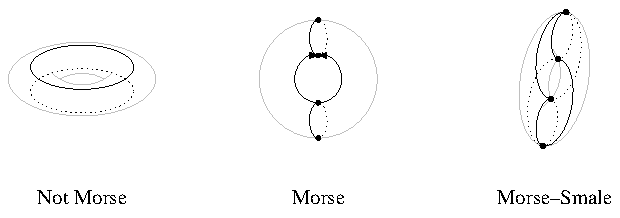
\includegraphics[width=0.82\textwidth]{figures/Fig_059_PDF138_Book126.pdf}
  \caption{高度函数分别不是 Morse 函数、是 Morse 函数及是 Morse--Smale 函数（原书 p.126）}
  \label{fig:morse-torus}
\end{figure}
\end{example}


现在设 $f$ 是 Morse--Smale 函数。若两个临界点 $p,q$ 的指数相差 $1$，则它们之间只有有限条流轨迹，因为此时 $\dim\operatorname{Desc}(p)\cap\operatorname{Asc}(q)=1$。可以按如下方式给每条轨迹赋予符号。先为所有 $\operatorname{Desc}(p)$ 选定定向；再要求分解
\[
  T_pM=T_p\operatorname{Desc}(p)\oplus T_p\operatorname{Asc}(p)
\]
保持定向，这便自动确定了 $\operatorname{Asc}(p)$ 的定向。类似地，可以为 $\operatorname{Desc}(p)\cap\operatorname{Asc}(q)$ 定向，方法是要求存在 $T_xM$ 的正向基 $b_1,\ldots,b_n$，使前一部分向量给出 $T_x\operatorname{Desc}(p)$ 的正向基，后一部分向量给出 $T_x\operatorname{Asc}(q)$ 的正向基，而重叠部分给出交空间 $T_x\operatorname{Desc}(p)\cap\operatorname{Asc}(q)$ 的正向基。

\begin{definition}{Morse 复形}{morse-complex}
紧致可定向 Riemann 流形 $(M,g)$ 上 Morse--Smale 函数 $f$ 的 Morse 复形\index{morsefuxing@Morse 复形|hyperpage} $C_M^\bullet(M,g,f)$，是由临界点张成、按 Morse 指数分次的向量空间。具体地，
\[
  C_M^i(M,g,f)=k\operatorname{Crit}_i(f),\qquad
  dp=\sum_{\substack{\gamma:p\to q\\|q|=|p|+1}}(-1)^\gamma q.
\]
这里 $(-1)^\gamma$ 在 $\gamma$ 沿 $\operatorname{Desc}(p)\cap\operatorname{Asc}(q)$ 的正向时取 $+1$。
\end{definition}

\begin{theorem}{Morse 复形计算流形上同调}{morse-cohomology}
Morse 复形是一个上链复形，并且它的上同调就是流形 $M$ 的上同调。
\end{theorem}
\begin{proof}[证明梗概]
微分的次数显然为 $1$，而且平方为零。展开 $d^2$ 可得
\[
  d^2(p)=\sum_{\substack{\gamma_1:p\to q\\|q|=|p|+1}}
  \sum_{\substack{\gamma_2:q\to r\\|r|=|q|+1}}
  (-1)^{\gamma_1}(-1)^{\gamma_2}r;
\]
因此，微分的平方统计了经由一个中间临界点到达 $r$ 的所有方式。

因为 $p$ 与 $r$ 的指数相差 $2$，$\operatorname{Desc}(p)$ 与 $\operatorname{Asc}(r)$ 的交是二维的。这意味着从 $p$ 到 $r$ 的轨迹组成单参数族；在这些单参数族的边界处，轨迹会断裂成两段。反过来，若有两条次数为 $1$ 的轨迹，局部上就可以把它们变形为一条次数为 $2$ 的轨迹。每个断裂为两段的轨迹族都有两个端点，因而总有两个符号相反的贡献，在 $d^2$ 中彼此抵消。下图示意这种边界配对：
\begin{figure}[H]\centering
  \centering
  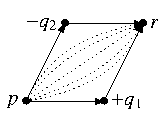
\includegraphics[width=0.32\textwidth]{figures/Fig_060_PDF139_Book127.pdf}
  \caption{一参数轨迹族的两种断裂端点（原书 p.127）}
  \label{fig:morse-broken-trajectories}
\end{figure}

为了证明 Morse 复形的上同调等于 $M$ 的上同调，把每个指数为 $i$ 的临界点与其上升流形对应起来。所有上升流形都是可缩的，并覆盖 $M$，因此给出一个胞腔分解；由此可以像定义单纯上同调那样定义胞腔上同调\bookcite[第 3 章]{111}。这个复形与 Morse 复形同构\bookcite[第 7.4 节]{28}。证明还有许多其他方法：使用同调而非上同调的论证见\bookcite[第 3 章]{123}；Witten\bookcite{256}则给出了完全不同的方法，把 Morse 复形与德拉姆复形联系起来。
\end{proof}

\begin{example}[驼峰球面的 Morse 复形]
考察一只竖立的、带有多个驼峰的球面。鞍点到两个驼峰各有一条路径，极小点到鞍点也有两条路径；后两条路径符号相反，因而彼此抵消。其 Morse 复形中，微分由鞍点映到两个极大点，而从极小点出发的两个贡献之和为 $1-1=0$。
若记极小点为 $p$、鞍点为 $q$，两个极大点为 $r_1,r_2$，则对应部分的微分为 $dp=(1-1)q=0$、$dq=r_1+r_2$。
\begin{figure}[H]\centering
  \centering
  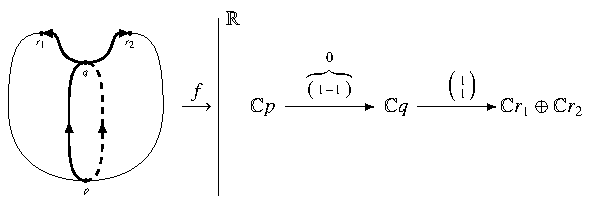
\includegraphics[width=0.72\textwidth]{figures/Fig_061_PDF140_Book128.pdf}
  \caption{驼峰球面上的临界点与 Morse 复形（原书 p.128）}
  \label{fig:morse-camel-sphere}
\end{figure}
\end{example}

\begin{note}\label{note:morse-homology-observation}
\textbf{观察 6.9.} 通过考察流形上函数的临界点所构成的复形，可以恢复流形的上同调；该复形的微分统计流轨迹。
\end{note}

\subsection{Morse 理论的动力学观点}\label{subsec:morse-dynamics}
现在用辛几何重新表述 Morse 理论。关于辛几何的背景，可参阅\bookcite{52,182}。回忆一下，辛流形是一个 $2n$ 维光滑实流形 $X$，带有闭且非退化的 $2$-形式 $\omega$：
\[
  d\omega=0,\qquad \omega(X,-)=0\Longrightarrow X=0.
\]
给定光滑函数 $h$，定义向量场 $X_h$ 使得
\[
  dh=\omega(-,X_h)=-\iota_{X_h}\omega,
\]
并定义流 $\phi_t^h\colon X\to X$，满足
\[
  \frac{d}{dt}\phi_t^h(x)=X_h(\phi_t^h(x)).
\]
函数 $h$ 通常称为 Hamilton 函数，该流称为 Hamilton 流\index{hamiltonliu@Hamilton 流|hyperpage}。Hamilton 流保持辛形式和 Hamilton 函数不变：
\[
  \frac{d}{dt}(\phi_t^h)^*\omega
  =\mathcal L_{X_h}\omega
  =\iota_{X_h}d\omega+d\iota_{X_h}\omega=0-d^2h=0,
\]
\[
  \frac{d}{dt}(\phi_t^h)^*h
  =\mathcal L_{X_h}h=dh(X_h)=\omega(X_h,X_h)=0.
\]
从物理角度看，Hamilton 函数表示系统总能量，而它在流下不变就意味着能量守恒。

辛流形的标准例子是流形 $M$ 的余切空间 $T^*M$，其上带有 $2$-形式
\[
  \omega=\sum_i dp_i\wedge dq_i,
\]
其中 $q_i$ 是 $M$ 上的局部坐标，$p_i$ 是余切空间中相对于基 $\{dq_i\}$ 的坐标。$q_i$ 称为位置坐标，$p_i$ 称为动量坐标。在这些坐标下，向量场 $X_h$ 的形式为
\[
  X_h=\sum_i\frac{\partial h}{\partial p_i}\frac{\partial}{\partial q_i}
       -\sum_i\frac{\partial h}{\partial q_i}\frac{\partial}{\partial p_i}.
\]

若 $f$ 是 Riemann 流形 $(M,g)$ 上的函数，可以沿投影映射将它拉回到 $T^*M$ 上。对应的 Hamilton 向量场为
\[
  X_f=-\sum_i\frac{\partial f}{\partial q_i}\frac{\partial}{\partial p_i}.
\]
% [Tutor Note: 符号约定需自行统一。原文 p.128 定义 $dh=\iota_{X_h}\omega$，但 p.129 的 $X_h=\sum_i\frac{\partial h}{\partial p_i}\frac{\partial}{\partial q_i}-\sum_i\frac{\partial h}{\partial q_i}\frac{\partial}{\partial p_i}$ 与 $\omega=\sum_i dp_i\wedge dq_i$ 差一负号；按已给的 $X_h$ 反推应为 $dh=\omega(-,X_h)=-\iota_{X_h}\omega$。后文例 6.56（原书 p.156）用 $\dot q_i=-\partial H/\partial p_i$、$\dot p_i=\partial H/\partial q_i$，即后一约定；推导 Floer 条带的 Cauchy--Riemann 方程时必须始终沿用同一约定。]
从物理角度看，这个动力系统颇为奇怪：粒子的动量会变化，但位置不变。这是因为 $f$ 含有势能项（依赖坐标 $q_i$），却不含动能项（依赖坐标 $p_i$）。流 $\phi_t^f$ 把底空间 $M\subset T^*M$ 移到另一个 $n$ 维子流形 $\phi_t^fM\subset T^*M$。$f$ 的临界点恰好是 $\phi_t^fM$ 与 $M$ 的交点，因为在这些点上流是静止的，即 $X_f(x)=0$。

若沿一条连接两个临界点的 Morse 轨迹 $\gamma$ 作流，它会扫出一个边界落在 $M\cup\phi_t^fM$ 上的曲面。这个曲面有一个特殊性质：它是全纯圆盘。为了说明这一点，先在 $T^*M$ 上定义复结构。切丛 $TM$ 有自然的复流形结构：若 $q_i$ 是 $M$ 上的局部坐标，则 $TM$ 上相对于局部基 $\frac{\partial}{\partial q_i}$ 的坐标为 $q_i,\dot q_i$；组合为
\[
  z_i=q_i+i\dot q_i
\]
便得到 $TM$ 上的全纯坐标。若 $M$ 带有度量 $g$，则切丛与余切丛之间有微分同胚
\[
  \phi_g\colon TM\to T^*M,\qquad X\longmapsto g(X,-).
\]
在该微分同胚下，坐标 $p_i$ 对应于 $g_{ij}\dot q_j$。这里使用 Einstein 求和约定，并记 $g_{ij}=g(\frac{\partial}{\partial q_i},\frac{\partial}{\partial q_j})$。

\begin{lemma}{Morse 轨迹给出全纯映射}{morse-trajectory-holomorphic}
映射
\[
  \psi\colon\mathbb R+[0,\epsilon]i\to T^*M,
  \qquad s+ti\longmapsto\phi_{t}^{h}\gamma(s)
\]
是全纯的。
\end{lemma}
\begin{proof}[证明梗概]
只需验证 Cauchy--Riemann 方程。沿 $s$ 方向的导数为 $(\nabla f,0)$，因为 $q_i$ 坐标沿 Morse 流变化，而 $p_i$ 不变。沿 $t$ 方向的导数只改变 $p_i$ 坐标，所以为 $\bigl(0,-\frac{\partial f}{\partial q_i}\bigr)$。改用 $(q_i,\dot q_i)$ 坐标后，得到
\[
  \frac{\partial\psi}{\partial s}=(\nabla f,0),\qquad
  \frac{\partial\psi}{\partial t}=(0,-\nabla f)
  =-i\frac{\partial\psi}{\partial s},
\]
这正是所需的 Cauchy--Riemann 方程。
\end{proof}

我们可以将条带 $\mathbb R+[0,\epsilon]i$ 全纯地识别为去掉 $\{1,-1\}$ 两点的单位圆盘 $D=\{z\in\mathbb C\mid|z|\le1\}$。于是 $\psi$ 可看成全纯映射
\[
  \psi\colon D\setminus\{-1,1\}\to T^*M,
\]
且当 $u\in[0,\frac12]$ 时 $\psi(e^{2\pi iu})\in M$，当 $u\in[\frac12,1]$ 时 $\psi(e^{2\pi iu})\in\phi_\epsilon^hM$。我们称这样的映射为全纯二边形（或双边形）。
\begin{figure}[H]\centering
  \centering
  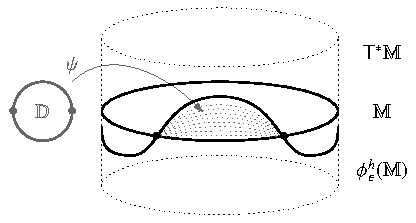
\includegraphics[width=0.62\textwidth]{figures/Fig_062_PDF142_Book130.pdf}\quad
  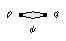
\includegraphics[width=0.22\textwidth]{figures/Fig_063_PDF142_Book130.pdf}
  \caption{Morse 流条带与余切丛中的全纯二边形（原书 p.130）}
  \label{fig:morse-holomorphic-bigon}
\end{figure}

从这个新观点看，Morse 上链复形由 $L:=\phi_\epsilon^hM$ 与 $M$ 的交点张成，而微分统计全纯二边形：
\[
  C_M^\bullet(M,g,f)=CF^\bullet(L,M)
  :=\bigoplus_{p\in L\cap M}kp,
  \qquad dp=\sum_{\substack{q\in L\cap M\\|q|=|p|+1}}
             \sum_{\psi:p\to q}\pm q.
\]

在这一新形式体系中，Morse 指数该如何解释？首先，若 $M$ 可定向，则可以给它配上体积形式
\[
  \Omega_{\mathbb R}=\sqrt{\det g_{ij}}\,dq_1\wedge\cdots\wedge dq_n.
\]
这个体积形式可在 $TM$ 上传递为复体积形式
\[
  \Omega_{\mathbb C}=\sqrt{\det g_{ij}}\,dz_1\wedge\cdots\wedge dz_n.
\]
考察它在 $T_pL$ 上的限制，像落在 $\mathbb C$ 中的一条直线 $\mathbb Re^{i\theta_p}$ 上，其中 $\theta_p\in\mathbb R/\pi\mathbb Z$。在此情形中，实际上可以把它提升为函数 $\theta_L\colon L\to\mathbb R$，这个提升函数称为分次。注意，$M$ 本身带有分次 $\theta_M\colon M\to\mathbb R$，其定义为 $p\mapsto0$，因为 $\Omega_{\mathbb C}|_{T_pM}$ 为实值。

若 $p$ 是 $L$ 与 $M$ 的交点，则存在酉变换 $U\colon T_p(T^*M)\to T_p(T^*M)$，把 $T_pL$ 映到 $T_pM$。取 $\Delta\in[0,\pi)$ 使 $\det U=\pm e^{i\Delta}$。交点 $p$ 的次数定义为
\[
  \deg p=\frac{\Delta-(\theta_M-\theta_L)}{\pi}.
\]
由于 $U^*(\Omega|_{T_pM})=\det(U)\,\Omega|_{T_pL}$，相位差 $\theta_M-\theta_L$ 必属于 $\Delta+\pi\mathbb Z$，所以 $\deg p$ 是整数。

\begin{example}[圆上的 Morse 函数与交点次数]
令 $M=\mathbb R/2\pi\mathbb Z$，取标准度量，并令 Hamilton 函数 $h=\cos q$。它在 $q=0,\pi$ 处有两个临界点 $p_0,p_1$。辛流形 $T^*M$ 是一个圆柱；除 $q=0,\pi$ 两处的静止轨迹外，其余轨迹都是竖直直线。
\begin{figure}[H]\centering
  \centering
  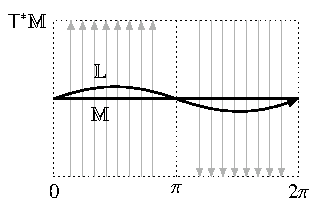
\includegraphics[width=0.78\textwidth]{figures/Fig_064_PDF143_Book131.pdf}
  \caption{圆的余切丛及 Hamilton 变形后的交点（原书 p.131）}
  \label{fig:circle-cotangent-flow}
\end{figure}
图中有两个拉格朗日子流形 $M$ 与其流动后的像 $L=\phi_\epsilon^h(M)$。$\theta_L$ 可取为 $T_pL$ 在每点处的相位，因此 $\theta_{p_0}=\epsilon$、$\theta_{p_1}=-\epsilon$。把 $T_pL$ 映到 $T_pM$ 的酉矩阵为
\[
  U_0=e^{i(\pi-\epsilon)},\qquad U_1=e^{i\epsilon},
\]
于是
\[
  \deg p_0=\frac{\pi-\epsilon-(0-\epsilon)}{\pi}=1,
  \qquad
  \deg p_1=\frac{\epsilon-(0+\epsilon)}{\pi}=0.
\]
\end{example}

\begin{note}\label{note:morse-intersections-observation}
\textbf{观察 6.12.} 通过考察余切丛中的零截面 $M\subset T^*M$ 与其 Hamilton 变形的交点，可以恢复流形的上同调；微分统计交点之间的全纯条带。
\end{note}

\subsection{环路空间的同调}\label{subsec:loop-space-homology}
现在考察动力学谱系的另一端，即 Hamilton 函数只有动能项的情形：
\[
  h=\frac12g^{ij}p_ip_j.
\]
这描述粒子在 $M$ 上自由运动。经典力学告诉我们，这种粒子以恒定速度沿 $M$ 上的测地线运动。在 $T^*M$ 的零截面 $M$ 上，$p_i=0$，所以速度为零，什么也不会发生：$\phi_\epsilon^h(M)=M$。

取余切丛的一条纤维 $L=T_x^*M$，并利用度量把它与 $T_xM$ 识别。点 $(q_i,\dot q_i)$ 在 $\phi_t^h$ 下的像，会沿 $\dot q_i$ 方向的测地线移动，距离为 $t\|\dot q_i\|$。

因此，$\phi_\epsilon^h(L)$ 与 $L$ 的交点表示从 $x$ 出发又回到 $x$ 的闭测地线。若 $\gamma\colon[0,1]\to M$ 是长度为 $\ell$ 的一条简单闭测地线，那么对任意 $z\in\mathbb Z$，点
\[
  \left(x,\frac{z\ell\,\dot\gamma(0)}{\epsilon\|\dot\gamma(0)\|}\right)
\]
都属于 $\phi_\epsilon^h(L)\cap L$；所有交点都由此方式得到。

考察以 $x$ 为基点的 $M$ 上所有环路组成的空间
\[
  \mathcal L_x(M)=\{\gamma\colon S^1\to M\mid\gamma(0)=x\}.
\]
环路空间上有函数 $f\colon\mathcal L_x(M)\to\mathbb R$，把每条环路映到其长度
\[
  f(\gamma)=\int_{S^1}\|\dot\gamma(t)\|\,dt.
\]
测地环路正是该函数的临界点，因此可以构造一个类似 Morse 复形的对象来计算 $\mathcal L_x(M)$ 的同调。它仍应由 $L$ 与 $\phi_t^h(L)$ 的交点张成。但此时交点不再来自静止轨迹，而来自周期轨迹。每个交点 $u$ 都对应一条从 $u$ 出发又回到 $u$ 的流线 $\widetilde\upsilon\colon[0,\epsilon]\to T^*M$。因此，微分应统计具有如下极限条件的条带：
\[
  \psi\colon\mathbb R+[0,\epsilon]i\to T^*M,
  \qquad s+ti\longmapsto\phi_t^h\gamma(s),
\]
其中 $s\to\pm\infty$ 时的极限恰好是上述流线。与 Morse 情形一样，这些条带应满足适当版本的 Cauchy--Riemann 方程。要使这一构造成立并不容易，因为无限维空间上的 Morse 理论技术性很强。

\begin{example}[圆周的环路空间]
令 $M=S^1$，则 $T^*M$ 是圆柱。标准坐标为 $(q,p)$，其中 $q$ 表示圆上的角度，$p$ 表示圆柱的高度。原点处的竖直线为 $L=T_0S^1$，而 $\phi_t^h(L)$ 是绕圆柱盘绕的螺线，其方程为 $q=tp$。交点为
\[
  (0,2\pi k/t),\qquad k\in\mathbb Z.
\]
环路空间按绕数分成连通分支，每个分支恰有一个临界点，所以不同临界点之间没有轨迹。因此，由 $\phi_t^h(L)$ 与 $L$ 的交点张成的复形，其微分为零。
\end{example}

\begin{note}\label{note:loop-space-intersections}
\textbf{观察 6.14.} 通过考察余切纤维 $T_x^*M$ 与其 Hamilton 变形的交点，可以计算流形环路空间的同调；微分统计交点之间的全纯条带。
\end{note}

\section{基本 Fukaya 范畴}\label{sec:basic-fukaya}
上面的讨论打开了若干推广方向。我们可以在任意辛流形中的拉格朗日子流形\index{lagelangriziliuxing@拉格朗日子流形|hyperpage}之间发展交理论，并通过考察全纯 $n$ 边形，把微分提升为高阶乘积。这就引出 Fukaya 范畴的思想。不过，Fukaya 范畴有许多不同概念，具体取决于辛流形的类型和要纳入的拉格朗日子流形种类。本节将定义最基本的版本，并详细讨论最简单的例子。

\takeaway{在带柱状端的 Liouville 流形中，正合紧致拉格朗日子流形之间的 Floer 复形由横截交点张成，高阶积通过计数满足边界条件的伪全纯多边形定义；正合性使求和有限并排除起泡，由此得到 $\mathbb Z_2$-分次的 $A_\infty$ 预范畴，存在复体积形式时可提升为 $\mathbb Z$-分次。}

\subsection{设定}\label{subsec:fukaya-setting}
为了得到合理的理论，当然需要限制辛流形与拉格朗日子流形的几何复杂度。因此，我们从一个与余切丛情形较为接近的设定开始。

\begin{definition}{Liouville 流形与 Liouville 域}{liouville-manifold}
若存在 $1$-形式 $\theta$ 使得 $\omega=d\theta$，则称辛流形 $(X,\omega)$ 为正合辛流形\index{zhenghexinliuxing@正合辛流形|hyperpage}。$1$-形式 $\theta$ 称为 Liouville 形式\index{liouvillexingshi@Liouville 形式|hyperpage}；满足 $\omega(X_\theta,-)=\theta$ 的向量场 $X_\theta$ 称为 Liouville 向量场\index{liouvillexiangliangchang@Liouville 向量场|hyperpage}。

若存在带边界的紧致流形 $X_0$ 满足以下条件，则称 $(X,\theta)$ 为具有柱状端的 Liouville 流形：
\begin{itemize}
  \item $X$ 由在 $X_0$ 的边界上接出柱体得到：
  \[
    X=X_0\cup_{\partial X_0}(\partial X_0\times[1,+\infty));
  \]
  \item 在柱体上，$X_\theta$ 指向外侧：
  \[
    X_\theta\big|_{\partial X_0\times[1,+\infty)}
    =r\frac{\partial}{\partial r},
  \]
  其中 $r$ 是 $(1,+\infty)$ 上的坐标。
\end{itemize}
紧致流形 $X_0$ 称为 Liouville 域\index{liouvilleyu@Liouville 域|hyperpage}\bookcite{15}。
\end{definition}

\begin{example}[余切丛上的 Liouville 结构]
带柱状端的 Liouville 流形\index{daizhuzhuangduandeliouvilleliuxing@带柱状端的 Liouville 流形|hyperpage}的标准例子是紧致流形 $M$ 的余切丛 $X=T^*M$。其 Liouville 形式为 $\theta=p_i\,dq_i$，相应的 Liouville 向量场为 $X_\theta=p_i\frac{\partial}{\partial p_i}$。$X_0$ 可取余切丛的单位球盘 $X_0=\{x\in X\mid\|p\|\le1\}$，坐标 $r$ 可取为 $\|p\|$（定义 $p$ 的范数时需要在 $M$ 上选取度量）。
\end{example}

\begin{definition}{正合拉格朗日子流形}{exact-lagrangian}\index{zhenghelagelangriziliuxing@正合拉格朗日子流形|hyperpage}
拉格朗日子流形是一个定向的 $n$ 维子流形 $L$，满足 $\omega(TL,-)=0$。若存在函数 $f\colon L\to\mathbb R$ 使得 $\theta|_L=df$，则称 $L$ 为正合的；若在柱体 $\partial X_0\times[1,+\infty)$ 上 Liouville 向量场 $X_\theta$ 与 $L$ 相切，则称 $L$ 具有锥形端\index{zhuixingduan@锥形端|hyperpage}。

若对每个交点 $p\in L_1\cap L_2$ 都有 $T_pX=T_pL_1\oplus T_pL_2$，则称两个拉格朗日子流形 $L_1,L_2$ 横截相交\index{hengjiexiangjiao@横截相交|hyperpage}。
\end{definition}

\begin{example}[余切丛中的零截面与纤维]
余切丛的底空间是紧致的正合拉格朗日子流形，而任意点 $x\in M$ 处的余切纤维是具有锥形端的正合拉格朗日子流形。两种情形下 $\theta$ 的限制都是零，因而是常值函数的微分。底空间与余切纤维在 $x$ 处横截相交。
\end{example}

\begin{definition}{相容的几乎复结构}{almost-kaehler}
给定 $2n$ 维辛流形 $(X,\omega)$，几乎复结构\index{jinfujiegou@几乎复结构|hyperpage}\index{fujiegou@复结构|hyperpage}是一个映射 $J\colon TX\to TX$，满足 $J^2=-1$。若
\[
  g(-,-):=\omega(-,J-)
\]
是 $X$ 上的 Riemann 度量，就称 $J$ 与 $\omega$ 相容。三元组 $(X,\omega,J)$ 称为几乎 Kähler 流形\index{khlerliuxing@Kähler 流形|hyperpage}。
\end{definition}

\begin{note}\label{note:almost-complex-structure}
\textbf{注 6.20.} 若 $X$ 是复流形（即存在坐标图 $\phi_U\colon U\to\mathbb C^n$，使得 $\phi_U\circ\phi_{U'}^{-1}$ 为全纯映射），就可以把 $X$ 看作实流形，并把映射 $J\colon TX\to TX:z\mapsto iz$ 看作几乎复结构。反过来通常不成立：并非每个几乎复结构都来自复坐标图册。若确实如此，就可以从定义中去掉“几乎”二字，称之为复结构，此时流形称为 Kähler 流形。
\end{note}

\begin{note}\label{note:compatible-almost-complex-contractible}
\textbf{注 6.21.} 对给定的 $(X,\omega)$，与 $\omega$ 相容的几乎复结构所成空间是可缩的。对所有复结构所成的空间，这一结论则不成立。
\end{note}

\begin{definition}{伪全纯映射}{pseudoholomorphic-map}
对任意开集 $U\subset\mathbb C$，若映射 $\phi\colon U\to X$ 满足 Cauchy--Riemann 方程
\[
  \frac{\partial\phi(u+iv)}{\partial u}
  +J\frac{\partial\phi(u+iv)}{\partial v}=0,
\]
则称 $\phi$ 为伪全纯映射\index{weiquanchunyingshe@伪全纯映射|hyperpage}。
\end{definition}

\begin{example}[复代数环面的 Liouville 结构]
\par
复代数环面 $(\mathbb C^*)^n$ 可通过 $z_i=e^{p_i+iq_i}$ 与 Liouville 流形 $(T^*(S^1)^n,p_i\,dq_i)$ 识别；这给出 $X=T^*(S^1)^n$ 上的复结构。因此 $(X,\omega,J)$ 是 Kähler 流形，并且
\[
  \omega=d\theta=\sum_i dp_i\wedge dq_i
  =\frac{i}{2}\sum_i d\ln z_i\wedge d\ln\bar z_i
  =\frac{i}{2}\sum_i\frac{dz_i}{z_i}\wedge\frac{d\bar z_i}{\bar z_i},
\]
\[
  J=\sum_i\left(i\frac{\partial}{\partial z_i}\otimes dz_i
   -i\frac{\partial}{\partial\bar z_i}\otimes d\bar z_i\right)
  =\sum_i\left(\frac{\partial}{\partial q_i}\otimes dp_i
   -\frac{\partial}{\partial p_i}\otimes dq_i\right),
  \qquad
  g=\sum_i(dp_i\otimes dp_i+dq_i\otimes dq_i).
\]
若 $f\in\mathbb C[X_1^{\pm1},\ldots,X_n^{\pm1}]$，且
\[
  X_f:=\{(z_1,\ldots,z_n)\in(\mathbb C^*)^n\mid f(z_1,\ldots,z_n)=0\}
\]
是光滑子流形，那么 $(X_f,\theta|_{X_f})$ 是带柱状端、具有相容复结构的 Liouville 流形。
\end{example}

\subsection{初步尝试定义 Fukaya 范畴}\label{subsec:fukaya-first-definition}
本节中，$(X,\theta)$ 表示带柱状端的 Liouville 流形。记 $\omega=d\theta$ 为其辛形式，并假设它带有一个相容的几乎复结构 $J$ 及其诱导度量 $g$。

\begin{definition}{Floer 复形与全纯多边形乘积}{floer-complex}
给定两个横截相交的紧致正合拉格朗日子流形 $L_1,L_2\subset X$，Floer 复形定义为 $\mathbb Z_2$-分次向量空间
\[
  CF_k^{\pm}(L_1,L_2):=\bigoplus_{p\in L_1\cap L_2}kp.
\]
交点 $p$ 的次数按如下方式确定。取 $T_pL_1$ 与 $T_pL_2$ 的正向基 $v_1,\ldots,v_n$ 和 $w_1,\ldots,w_n$。若 $v_1,\ldots,v_n,w_1,\ldots,w_n$ 构成 $T_pX$ 的正向基，则令 $\deg p=0$；若它构成负向基，则令 $\deg p=1$。
设 $L_0,\ldots,L_k$ 是两两横截相交的紧致正合定向拉格朗日子流形，则定义
\[
  \mu\colon CF_k^{\pm}(L_1,L_0)\otimes\cdots\otimes
    CF_k^{\pm}(L_k,L_{k-1})\to CF_k^{\pm}(L_k,L_0)
\]
为
\[
  \mu(p_1,\ldots,p_k):=\sum_{p_0\in L_0\cap L_k}\sum_{\psi}
     \sigma_\psi\,p_0.\tag{6.1}\label{eq:fukaya-product}
\]
这里对所有满足下列条件的伪全纯映射
\[
  \psi\colon D\setminus\{e^{2r\pi i/(k+1)}\mid r\in\mathbb Z\}\to X
\]
求和：
\begin{itemize}
  \item 边界映到拉格朗日子流形上：若 $t\in(i,i+1)$，则 $\psi(e^{2\pi it/(k+1)})\in L_i$；
  \item 在单位根 $\zeta_r=e^{2r\pi i/(k+1)}$ 处的极限对应交点，即 $\lim_{t\to\zeta_r}\psi(z)=p_r$；
  \item 映射按固定各 $\zeta_r$ 的圆盘重参数化取等价类；
  \item 映射不能再作形变；
  \item 每一项都带有符号 $\sigma_\psi$，该符号取决于拉格朗日子流形的定向，也可能取决于其他附加数据。
\end{itemize}
图示如下；每个交点处的小箭头表示相应态射的方向：
\begin{figure}[H]\centering
  \centering
  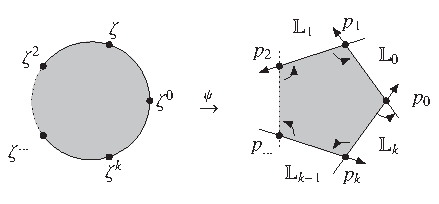
\includegraphics[width=0.66\textwidth]{figures/Fig_065_PDF148_Book136.pdf}
  \caption{由全纯多边形定义高阶乘积（原书 p.136）}
  \label{fig:fukaya-holomorphic-polygons}
\end{figure}
\end{definition}

从图像上看，这类映射可画成边界依次落在各拉格朗日子流形上的圆盘，并在各角点处标出态射方向。目标空间的角点刻意画成非光滑的形状，以强调 $\psi$ 在 $\zeta_i$ 处不必全纯。若拉格朗日子流形是一维的，那么对每个次数为奇数且 $i>0$ 的 $p_i$，当其目标拉格朗日子流形的正向与圆盘边界的正向相反时，$\sigma_\psi$ 会多出一个 $-1$ 因子。

我们希望这些乘积定义良好并满足 $A_\infty$ 关系；但要做到这一点，还必须处理若干技术问题。

\subsection{模空间}\label{subsec:fukaya-moduli-spaces}
首先要精确说明“映射不能再作形变”是什么意思。给定交点序列 $p_0,\ldots,p_k$，可以构造模空间 $\mathcal M(p_0,\ldots,p_k)$，其元素是满足相应边界条件的映射，按重参数化取等价类。模空间自然按 $\psi$ 相对于边界 $\bigcup_iL_i$ 的同调类分解为不交并：
\[
  \mathcal M(p_0,\ldots,p_k)=
  \coprod_{u\in H_2(X,\cup_iL_i)}\mathcal M_u.
\]
理想情况下，每个 $\mathcal M_u$ 都应当是维数等于预期维数的光滑可定向流形；然而，这并不容易做到。
\begin{itemize}
  \item 为保证光滑性，必须假设 $J$ 是通有的；甚至可能要通过加入依赖时间的 Hamilton 流和几乎复结构来扰动 Cauchy--Riemann 方程。这类似于构造 Morse 复形时要求函数为 Morse--Smale 函数。
  \item 为保证可定向性，拉格朗日子流形需要可定向，并带有自旋结构\bookcite[II.11]{218}。若 $L$ 是闭曲线，它有两种自旋结构：平凡自旋结构与非平凡自旋结构，分别对应圆上的两种局部 $\mathbb Z_2$-系。非平凡自旋结构可通过在曲线上选取一个标记点来描述，在该点处平凡化失效。圆盘边界上的每个标记点都会在 $\sigma_\psi$ 中额外引入一个负号。
\end{itemize}

下文中我们假设 $\mathcal M_u$ 是可定向流形。当 $\dim\mathcal M_u=0$ 时，它是由离散点 $\psi$ 组成的集合，每个点带有表示定向的符号 $\sigma_\psi$。我们只对零维 $\mathcal M_u$ 中的映射求和。

为了保证上述定义良好，参与求和的映射 $\psi$ 总数必须有限。这一点并不显然：即使每个零维 $\mathcal M_u$ 都只含有限多个点，它们的总数仍可能无限。幸运的是，我们施加的限制可以帮助解决这个问题。

\begin{lemma}{正合性保证 Floer 乘积有限}{exactness-finite-floer-sum}
若辛流形及所有紧致拉格朗日子流形都是正合的，则式~\eqref{eq:fukaya-product} 中的和是有限和。
\end{lemma}
\begin{proof}[证明梗概]
这要用到 Gromov 紧致性定理\bookcite{100}：给定面积上界后，面积小于该上界的全纯映射只有有限多个。由于 $\omega$ 正合，映射 $\psi$ 的面积可表示为边界上的积分，再拆成各拉格朗日子流形上的积分之和：
\[
  \int_D\psi^*\omega=\int_Dd\psi^*\theta
  =\int_{\partial D}\psi^*\theta
  =\sum_i\int_{p_i}^{p_{i+1}}\theta|_{L_i}.
\]
由正合性，每一项都可写成
\[
  \int_{p_i}^{p_{i+1}}\theta|_{L_i}
  =\int_{p_i}^{p_{i+1}}df_i=f_i(p_{i+1})-f_i(p_i),
\]
其中 $f_i\colon L_i\to\mathbb R$ 是 $\theta|_{L_i}$ 的原函数。因为 $L_i$ 紧致，积分被 $f_i$ 的最大值与最小值之差控制，因此 $\psi$ 的面积有界。
\end{proof}

\subsection{泡}
为了确保这些乘积满足 $A_\infty$ 关系，我们希望仿照定理~\ref{thm:morse-cohomology} 中 Morse 微分的情形。在那里，我们把两条轨迹粘在一起，再将它们变形为一个单参数族；这个轨迹族的断裂端点对应另外一对轨迹，而这两端的贡献在 $d^2$ 中相消。

这里也可以做类似的事：把两个圆盘沿一个共同标记点粘合起来，对粘合结果作形变，再使它断裂为另外两个圆盘。形变族的两个端点分别对应 $A_\infty$ 关系中的项，例如 $\mu_1(\mu_4(p_1,\ldots,p_4))$ 和 $\mu_3(p_1,\mu_2(p_2,p_3),p_4)$；它们符号相反，因而相消。

至少理论上应当如此；但实际上还会出现两类退化，它们并不对应 $A_\infty$ 公理中的项。这种现象称为起泡\index{qipao@起泡|hyperpage}：
\begin{itemize}
  \item \textbf{圆盘泡}\index{yuanpanpao@圆盘泡|hyperpage}发生在额外圆盘从某段边界冒出时。该圆盘可看作零元乘积 $\mu_0$ 的额外贡献；此时得到的不是普通 $A_\infty$ 结构，而是带曲率的 $A_\infty$ 结构。
  \item \textbf{球面泡}\index{qiumianpao@球面泡|hyperpage}发生在球面从圆盘内部切离时。
\end{itemize}
泡类似于含有环路的 Morse 轨迹。在 Morse 理论中，由于轨迹沿 Morse 函数单调上升，这种情形不可能发生。正合情形下也可以得到类似结论。
\begin{figure}[H]\centering
  \centering
  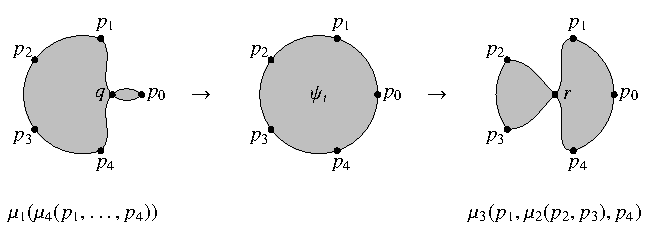
\includegraphics[width=0.78\textwidth]{figures/Fig_066_PDF150_Book138.pdf}
  \caption{模空间边界上的断裂圆盘（原书 p.138）}
  \label{fig:fukaya-moduli-boundary}
\end{figure}
\begin{figure}[H]\centering
  \centering
  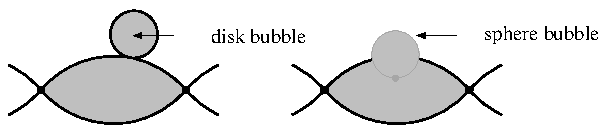
\includegraphics[width=0.58\textwidth]{figures/Fig_067_PDF150_Book138.pdf}
  \caption{圆盘泡与球面泡（原书 p.138）}
  \label{fig:fukaya-disk-sphere-bubbles}
\end{figure}

\begin{lemma}{$A_\infty$ 关系}{fukaya-ainfty-relations}
乘积 $\mu_k$ 满足 $A_\infty$ 公理。
\end{lemma}
\begin{proof}[证明梗概]
在正合情形下，两类泡都会给出面积为零的映射 $\psi$。利用这些映射可以构造出无穷多个面积受某个常数控制的映射，这与 Gromov 紧致性定理矛盾。

完整证明见 Seidel\bookcite[第二部分]{218}。证明中要构造模空间 $\mathcal M_u(p_0,\ldots,p_k)$ 的紧化，其边界由含有较少标记点的模空间之积构成。在这些空间上，$A_\infty$ 乘积可解释为边界算子 $d$，于是 $A_\infty$ 关系便来自 $d^2=0$。
\end{proof}
% [Tutor Note: “$J$ 一般”只保证模空间在预期维数处光滑，这里省略了两处：一是标记点处的赋值映射也须横截，否则要用含时 Hamilton 扰动或虚拟基本类框架；二是正合性只排除面积为零的泡，还须先证明面积有正下界，才能由 Gromov 紧致性得到有限性。完整细节见 Seidel 书第二部分（文献 218）。]

\subsection{Floer 上同调}\label{subsec:floer-cohomology}
处理好上述问题后，便得到 Floer 理论的基本定理。

\begin{theorem}{Floer 上同调不变性}{floer-invariance}
（Floer\bookcite{79}）设 $k$ 是特征为 $2$ 的域，$(X,\theta,J)$ 是带柱状端的 Liouville 流形，并带有相容的几乎复结构。设 $L_1,L_2$ 是紧致、正合、定向的拉格朗日子流形，二者横截相交，并假设 $J$ 通有。
\begin{enumerate}[label=(\roman*)]
  \item $(CF_k^{\pm}(L_1,L_2),\mu_1)$ 是一个 $\mathbb Z_2$-分次复形。
  \item 若 $J_t$（$t\in[0,1]$）是一族几乎复结构，那么只要 $J_0,J_1$ 通有，就有拟同构
  \[
    CF_k^{\pm}(L_1,L_2)_{J_0}\simeq CF_k^{\pm}(L_1,L_2)_{J_1}.
  \]
  \item 若 $\phi_t^h$ 是 Hamilton 流，那么只要所涉及的拉格朗日子流形横截相交，就有拟同构
  \[
    CF_k^{\pm}(L_1,L_2)\simeq
    CF_k^{\pm}(\phi_\epsilon^hL_1,L_2)\simeq
    CF_k^{\pm}(L_1,\phi_\epsilon^hL_2).
  \]
\end{enumerate}
换言之，Floer 上同调是一个不变量，只依赖于拉格朗日子流形的 Hamilton 同痕类和辛结构。
\end{theorem}

\begin{note}\label{note:floer-spin-structure}
\textbf{注 6.29.} 如前所述，若要使该定理对特征不为 $2$ 的域成立，拉格朗日子流形必须配备自旋结构\bookcite[II.11]{218}。
\end{note}

\subsection{预范畴}\label{subsec:fukaya-precategories}
现在希望把这些数据打包成一个范畴。对象应是 $X$ 中正合、紧致的拉格朗日子流形，态射空间应为 Floer 复形。遗憾的是，事情没有这么简单：态射空间只在横截相交的拉格朗日子流形之间定义，因此对象与自身之间尤其没有态射空间。第三章第 3.4.4 节介绍的预范畴可以解决这个问题。

\begin{definition}{基本 Fukaya 预范畴}{basic-fukaya-precategory}
设 $(X,\theta,J)$ 是带柱状端的 Liouville 流形，并带有相容的几乎复结构。基本 Fukaya 预范畴 $\widehat{\mathrm{Fuk}}^{\pm}(X,\theta,J)$ 是具有下列数据的 $\mathbb Z_2$-分次预范畴：
\begin{itemize}
  \item 对象是 $X$ 中配有自旋结构的紧致、定向、正合拉格朗日子流形；
  \item 横截序列由满足以下条件的拉格朗日子流形元组组成：元组中各子流形两两横截相交、交点各不相同，且 $J$ 通有；
  \item 对每个 $(L_1,L_2)\in\widehat{\mathrm{Fuk}}^{\pm}(X,\theta,J)^2_{\mathrm{tr}}$，置
  \[
    \widehat{\mathrm{Fuk}}^{\pm}(L_1,L_2)=CF_k^{\pm}(L_1,L_2);
  \]
  \item 对每个 $(L_0,\ldots,L_k)\in\widehat{\mathrm{Fuk}}^{\pm}(X,\theta,J)^{k+1}_{\mathrm{tr}}$，定义前文给出的乘积 $\mu_k$。
\end{itemize}
\end{definition}

\begin{lemma}{基本 Fukaya 预范畴具有足够多拟同构}{fukaya-precategory-quasi-isomorphisms}
$\widehat{\mathrm{Fuk}}^{\pm}(X,\theta,J)$ 是一个具有足够多拟同构的预范畴。
\end{lemma}
\begin{proof}[证明梗概]
横截序列的任意子序列仍是横截的；又因为这里不会起泡，所以只要 $A_\infty$ 公理中的乘积有定义，这些公理就成立。

为证明它具有足够多拟同构，设 $L$ 是紧致拉格朗日子流形。由\bookcite[6.1]{252}可知，$L\subset X$ 的一个邻域与 $T^*L$ 同构。若在 $L$ 上选取一个 Morse--Smale 函数 $f$，并使每个连通分支上恰有一个局部极小值，就可以用该函数把 $L$ 流到 $\phi_\epsilon^fL$。这些极小值之和给出 $\widehat{\mathrm{Fuk}}^{\pm}(L,\phi_\epsilon^fL)$ 中的一个零次态射，它对应于
\[
  H^\bullet(L,k)\cong HCF_k^\bullet(L,\phi_\epsilon^fL)
\]
中的单位，因此是拟同构。

由于 $f$ 可以是 $L$ 上任意 Morse--Smale 函数，这样的拟同构有很多。给定其他一组拉格朗日子流形后，总能找到一个 $f$，使 $L_+=\phi_\epsilon^fL$ 与 $L_-=\phi_{-\epsilon}^fL$ 都和它们横截相交，并与 $J$ 相容。
\end{proof}

\begin{definition}{基本 Fukaya 范畴}{basic-fukaya-category}
基本 Fukaya 范畴 $\widehat{\mathrm{Fuk}}^{\pm}(X,\theta,J)$ 定义为相应基本 Fukaya 预范畴的范畴化。
\end{definition}

\begin{theorem}{基本 Fukaya 范畴与几乎复结构无关}{fukaya-complex-structure-invariance}
对两个不同的几乎复结构 $J_0,J_1$，Fukaya 范畴 $\widehat{\mathrm{Fuk}}^{\pm}(X,\theta,J_0)$ 与 $\widehat{\mathrm{Fuk}}^{\pm}(X,\theta,J_1)$ 之间存在 $A_\infty$ 拟同构。
\end{theorem}
\begin{proof}[证明梗概]
几乎复结构空间是可缩的，因此可以构造一条从 $J_0$ 到 $J_1$ 的路径 $\gamma$。仿照定理~\ref{thm:floer-invariance}，该路径在 $CF_k^{\pm}(L_1,L_2)_{J_0}$ 与 $CF_k^{\pm}(L_1,L_2)_{J_1}$ 之间诱导拟同构；它们可以提升为预范畴之间的 $A_\infty$ 函子，并在导出范畴上诱导拟等价。
\end{proof}

\begin{example}[圆柱上的 Fukaya 范畴]
取 $X=T^*S^1$，令 $\theta=p\,dq$，并把 $X$ 与 $\mathbb C/2\pi\mathbb Z$ 等同起来，以定义复结构 $J$。若嵌入 $L\subset X$ 是正合的，则其切空间不可能竖直。这意味着 $L$ 的每个连通分支都是形如 $p\colon\mathbb R\to\mathbb R$ 的 $2\pi$-周期函数的图像。

这样的函数给出正合嵌入，当且仅当 $p$ 是某个 $2\pi$-周期原函数 $f$ 的导数；等价地，$\int_0^{2\pi}p(t)\,dt=0$。注意，任意两个这样的嵌入总会相交，因此 $L$ 只能有一个连通分支。该分支可以有两种定向，取决于我们沿嵌入圆的正向还是反向行进。于是得到双射
\[
  \operatorname{Ob}\widehat{\mathrm{Fuk}}^{\pm}(X)
  \longleftrightarrow
  \{df\mid f\colon S^1\to\mathbb R\}\times\{+,-\}.
\]

取两个横截相交的拉格朗日嵌入 $L_1,L_2$。若它们相交于 $2r$ 个点，就根据 $L_2$ 是从 $L_1$ 下方还是上方穿过，把交点记作 $u_i,v_i$。若 $L_1,L_2$ 定向相同，则 $u_i$ 的 $\mathbb Z_2$ 次数为 $0$，$v_i$ 的次数为 $1$；若定向相反，次数互换。
\begin{figure}[H]\centering
  \centering
  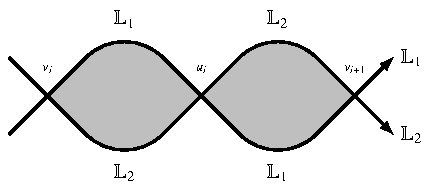
\includegraphics[width=0.72\textwidth]{figures/Fig_068_PDF153_Book141.pdf}
  \caption{圆柱上两条拉格朗日曲线的交点与次数（原书 p.141）}
  \label{fig:cylinder-lagrangians-intersections}
\end{figure}

从某个 $u$ 到相邻的 $v$ 恰有一条全纯条带。后一侧的条带带正号，前一侧的条带带负号：
\[
  CF_k^{\pm}(L_1,L_2)=\bigoplus_{i=1}^r(ku_i\oplus kv_i),
  \qquad \mu_1(u_i)=v_{i+1}-v_i.
\]
该复形的上同调由 $\iota=\sum_i u_i$ 与 $\xi=v_1$ 张成（在上同调中也可以用任意 $v_i$ 代替 $v_1$，因为它们彼此相等）。转到极小模型后，对每一对横截曲线都有
\[
  H\widehat{\mathrm{Fuk}}^{\pm}(L_1,L_2)
  =k\iota^{[12]}\oplus k\xi^{[12]}.
\]

为了将这个预范畴范畴化，注意每个 $\iota^{[12]}$ 都是拟同构。事实上，若 $u^{[13]}\colon L_1\to L_3$ 是一个零次交点，它恰好位于一个由零次交点构成的三角形中；该三角形由 $L_1$ 上先于它的 $u^{[12]}$ 和 $L_2$ 上后于它的 $u^{[23]}$ 张成，或者在 $L_2$ 位于 $u^{[13]}$ 上方或下方时反过来。因此有
\[
  \iota^{[23]}\iota^{[12]}=\iota^{[13]}.
\]
\begin{figure}[H]\centering
  \centering
  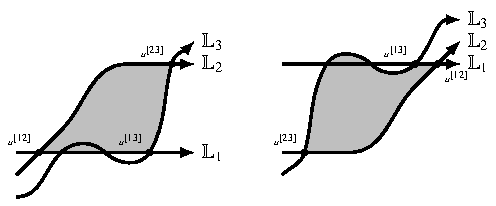
\includegraphics[width=0.74\textwidth]{figures/Fig_069_PDF154_Book142.pdf}
  \caption{零次交点的三角形乘积（原书 p.142）}
  \label{fig:cylinder-triangle-product}
\end{figure}
类似地，可以推出
\[
  \xi^{[23]}\iota^{[12]}=\iota^{[23]}\xi^{[12]}=\xi^{[13]},
  \qquad \xi^{[23]}\xi^{[12]}=0.
\]
范畴化之后，定向相同的所有对象都彼此同构，所有 $\iota$ 都成为单位。经过一次 $A_\infty$ 同构，可以把它们化为严格单位。这意味着，可能非零的高阶乘积只涉及 $\xi$。然而，若考察由同一方向绕圆柱的拉格朗日子流形围成的任意 $n$ 边形，它们不可能都沿着多边形的同一方向行进。于是至少有两处方向发生改变，这两处中至少一处会在乘积中出现为一个 $\iota$，因此
\[
  \mu(\xi,\ldots,\xi)=0.
\]
\begin{figure}[H]\centering
  \centering
  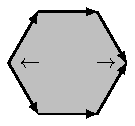
\includegraphics[width=0.28\textwidth]{figures/Fig_070_PDF154_Book142.pdf}
  \caption{沿圆柱同向绕行的多边形必有方向转折（原书 p.142）}
  \label{fig:cylinder-polygon-direction}
\end{figure}

由此可知，Fukaya 范畴等价于一个普通的 $\mathbb Z_2$-分次范畴，它有两个对象 $\{L_+,L_-\}$，且
\[
  \begin{aligned}
  \widehat{\mathrm{Fuk}}^{\pm}(L_+,L_+)
  &=\widehat{\mathrm{Fuk}}^{\pm}(L_-,L_-)
   =k[\xi]/(\xi^2)=\Lambda_1^{\pm},\\
  \widehat{\mathrm{Fuk}}^{\pm}(L_+,L_-)
  &=\widehat{\mathrm{Fuk}}^{\pm}(L_-,L_+)
   =k[\xi]/(\xi^2)[1]=\Lambda_1^{\pm}[1].
  \end{aligned}
\]
取导出版本，则
\[
  D\widehat{\mathrm{Fuk}}^{\pm}(X,\theta,J)\cong_\infty D\Lambda_1^{\pm}.
\]
\end{example}

\subsection{提升分次}\label{subsec:upgrade-grading}
在前面的构造中，我们只给范畴赋予了 $\mathbb Z_2$-分次，但有时也可以构造 $\mathbb Z$-分次范畴。理想情况下，要全面讨论 Fukaya 范畴的分次，应当介绍 Maslov 指数\bookcite{12,173,238}；它是 Floer 理论中 Morse 指数的推广。不过，这里我们采用与第~\ref{subsec:morse-dynamics} 节一致的较基础方法。

\begin{definition}{Calabi--Yau 流形}{calabi-yau-manifold}
Calabi--Yau 流形\index{calabiyauliuxing@Calabi–Yau 流形|hyperpage} $(X,\Omega)$ 是一个 Kähler 流形 $(X,\omega,J)$，配有处处不为零的复体积形式 $\Omega\in\Omega^n_{\mathbb C}(X)$。
\end{definition}

与第~\ref{subsec:morse-dynamics} 节的讨论类似，可以利用这个体积形式定义分次拉格朗日子流形\index{fencilagelangriziliuxing@分次拉格朗日子流形|hyperpage}，并给 Floer 复形赋予分次。

\begin{definition}{$\Omega$-分次拉格朗日子流形}{omega-graded-lagrangian}
$\Omega$-分次拉格朗日子流形是一个二元组 $(L,\theta)$，其中 $L$ 是拉格朗日子流形，$\theta\colon L\to\mathbb R$ 是函数，并且 $e^{-i\theta}\Omega$ 是 $L$ 上的实体积形式。若 $L$ 可由常值函数赋予分次，则称它为特殊拉格朗日子流形\index{teshulagelangriziliuxing@特殊拉格朗日子流形|hyperpage}。
\end{definition}

并非每个拉格朗日子流形都可以赋予分次。对每个 $x\in L$，$\theta(x)$ 都只确定到相差 $\pi$ 的整数倍。若在 $x$ 处固定 $\theta$，并沿曲线 $\gamma\colon x\to y$ 延拓，就能得到 $\theta(y)$；要使 $L$ 可分次，这个延拓结果必须与路径选择无关。若 $L$ 连通且可分次，那么每个 $k\in\mathbb Z$ 恰好对应一个分次，因为两个分次全局相差 $\pi$ 的整数倍。分次会自动给拉格朗日子流形定向：取 $e^{-i\theta}\Omega$ 作为实体积形式即可。相差奇数倍 $\pi$ 的两个分次给出相反定向。

\begin{definition}{分次交点的次数}{graded-intersection-degree}
设两个带分次的拉格朗日子流形 $(L_1,\theta_1)$ 和 $(L_2,\theta_2)$ 在 $x$ 处横截相交。取一个相对于几乎复结构 $J$ 的酉映射 $U\colon T_xX\to T_xX$，使得 $U(T_xL_1)=T_xL_2$，并选取 $\Delta\in[0,\pi)$ 使 $\det U=\pm e^{i\Delta}$。定义 Floer 复形 $CF_k^\bullet(L_1,L_2)$ 中交点 $x$ 的次数为
\[
  \deg x=\frac{\Delta-(\theta_2(x)-\theta_1(x))}{\pi}.
\]
\end{definition}

\begin{lemma}{分次交点次数与乘积次数}{graded-fukaya-product-degree}
交点 $x$ 的次数定义良好，且乘积 $\mu_k$ 的次数为 $2-k$。
\end{lemma}
\begin{proof}[证明梗概]
首先，$\deg x$ 是整数，因为
$U^*(\Omega|_{T_xL_2})=\det(U)\,\Omega|_{T_xL_1}$，从而
$\Delta-(\theta_2(x)-\theta_1(x))$ 是 $\pi$ 的整数倍。其定义也与 $U$ 的选取无关，因为 $U$ 只在左右乘上固定 $T_xL_1$ 或 $T_xL_2$ 的酉变换时才会改变；这些变换在对应子空间上都是正交变换，故行列式为 $\pm1$。

为了求 $\mu_k$ 的次数，可以把每个伪全纯映射的定义域从圆盘变换为内角为相应 $\Delta$ 的凸多边形。结论便由 $k$ 边形内角和为 $(k-2)\pi$ 得出。
\end{proof}
% [Tutor Note: $\Delta$ 取的是 Maslov 指数模 $\pi$ 的代表元：公式给出 $\mathbb Z$-次数，模 $2$ 即得先前的 $\mathbb Z_2$-次数。$U$ 只确定到左乘、右乘分别固定 $T_xL_1$、$T_xL_2$ 的正交变换，其行列式为 $\pm1$，故 $\Delta$ 的模 $\pi$ 约化与 $\deg x$ 均与 $U$ 的选取无关；实际计算时务必先固定 $L_1,L_2$ 的定向与分次。]

\begin{definition}{整数分次基本 Fukaya 范畴}{z-graded-basic-fukaya}
$\mathbb Z$-分次基本 Fukaya 预范畴 $\widehat{\mathrm{Fuk}}^\bullet(X,\Omega)$ 的横截序列，由满足以下条件的 $\Omega$-分次拉格朗日子流形组成：它们两两横截相交、紧致、正合，并带有自旋结构；其 Hom 空间是相应的 $\Omega$-分次 Floer 复形，乘积则仍按前述方式定义。$\mathbb Z$-分次 Fukaya 范畴 $\widehat{\mathrm{Fuk}}^\bullet(X,\Omega)$ 是该预范畴的范畴化。
\end{definition}

整数分次 Fukaya 预范畴依赖于 $\Omega$，但不同的 $\Omega$ 也可能给出同构范畴。若存在一条由复体积形式构成的路径连接 $\Omega_0$ 与 $\Omega_1$，就称它们同伦。

\begin{lemma}{同伦复体积形式给出同构预范畴}{homotopic-volume-forms}
同伦的复体积形式诱导同构的 Fukaya 预范畴。
\end{lemma}
\begin{proof}[证明梗概]
设 $\Omega_t$（$t\in[0,1]$）是连接两者的路径。对每个点 $x$，可以计算 $\Omega_t(x)$ 的相位沿该路径变化了多少：
\[
  \vartheta(x)=\int_0^1d\arg\Omega_t(x).
\]
若 $\theta\colon L\to\mathbb R$ 是 $\Omega_0$-分次，那么 $\theta-\vartheta$ 就是 $\Omega_1$-分次，反之亦然。因此，$\Omega_0$-分次与 $\Omega_1$-分次拉格朗日子流形之间存在双射。由这些分次诱导的 Floer 复形分次相同，因为相位项 $\vartheta$ 会相消。
\end{proof}

\begin{example}[圆柱上的整数分次]
利用坐标 $z=e^{p+qi}$，可以把 $X=T^*S^1$ 识别为 $\mathbb C^*$。复体积形式是处处不为零的 $1$-形式，例如 $\Omega=z^r\,dz$。要给底拉格朗日子流形 $S^1$ 赋予分次，必须取
\[
  \theta(q)=-rq-q+k\pi.
\]
除非 $r=-1$，否则该函数不具周期性，因此不是定义在圆上的函数。

这意味着，除非 $\Omega=dz/z$，整数分次基本 Fukaya 范畴为空。在此情形下，它等价于一个对象为 $L[k]$（$k\in\mathbb Z$）的范畴；这些对象对应分次拉格朗日子流形 $(S^1,k\pi)$，且
\[
  \widehat{\mathrm{Fuk}}^\bullet(L[i],L[j])
  =k[\xi]/(\xi^2)[j-i]=\Lambda_1^\bullet[j-i].
\]
在导出层面可得
\[
  D\widehat{\mathrm{Fuk}}^\bullet\left(\mathbb C^*,\frac{dz}{z}\right)
  \cong_\infty D\Lambda_1^\bullet\cong_\infty D\mathrm{mod}^\bullet k[[X]].
\]
\end{example}

\section{变体}\label{sec:fukaya-variations}
现在构造一些 Fukaya 型范畴，它们是前一构造的不同变体。每个变体都有两种版本：若存在复体积形式 $\Omega$，则有 $\mathbb Z$-分次版本；否则只有 $\mathbb Z_2$-分次版本。为避免重复和记号繁杂，下文省略 $\Omega$，但范畴记号采用 $\mathbb Z$-分次版本。

\takeaway{基本构造可扩充为多种变体：纳入浸入与局部系统；用 Reeb 弦与带结的圆盘定义 wrapped Fukaya 范畴；用 stop 截断 Reeb 流得到 partially wrapped 范畴；以 Lefschetz 纤维化的 thimble 定义有向 Fukaya 范畴；并借除子与 Novikov 域处理紧致流形的相对与完整 Fukaya 范畴。}

\subsection{浸入与局部系统}\label{subsec:immersions-local-systems}
可以从两个方向扩充 Floer 上同调的适用范围：允许拉格朗日子流形是浸入的，并在拉格朗日子流形上配置局部系统。

\begin{definition}{带局部系统的浸入拉格朗日子流形}{lagrangian-brane}
带局部系统的浸入拉格朗日子流形（也称拉格朗日膜\index{lagelangrimo@拉格朗日膜|hyperpage}）是三元组 $(L,\mathcal L,\phi)$，其中：
\begin{itemize}
  \item $L$ 是一个 $n$ 维紧致定向流形（若 $\operatorname{char}k\ne2$，还须带有自旋结构）；
  \item $\mathcal L\colon\Pi_1(L)\to\mathrm{vect}(k)$ 是一个局部系统；
  \item $\phi\colon L\to X$ 是浸入，且对所有 $p\in L$，$\phi_*T_pL$ 都是拉格朗日子空间。
\end{itemize}
此外，我们要求浸入的自交是横截的：$L$ 中至多两个点映到 $X$ 中的同一点；若 $\phi(p_1)=\phi(p_2)=x$，则
\[
  T_xX=\phi_*T_{p_1}L\oplus\phi_*T_{p_2}L.
\]
这样的点称为双点。若存在 $f\colon L\to\mathbb R$ 使 $\phi^*\theta=df$，则称该浸入正合。
\end{definition}

若正合拉格朗日膜 $L_i:=(L_i,\mathcal L_i,\phi_i)$ 两两横截相交，且交点不是双点，则可定义 Floer 复形
\[
  CF_k^\bullet(L_1,L_2)=
  \bigoplus_{p\in\phi_1(L_1)\cap\phi_2(L_2)}
  \mathrm{Hom}_k\!\left(\mathcal L_1(\phi_1^{-1}p),
                        \mathcal L_2(\phi_2^{-1}p)\right)\,p.
\]
乘积变为
\[
  \begin{aligned}
  \mu(\alpha_1p_1,\ldots,\alpha_kp_k)
  :=\sum_{p_0\in\phi_0(L_0)\cap\phi_k(L_k)}\sum_\psi
  &\mathcal L_0(\gamma_0)\alpha_1\mathcal L_1(\gamma_1)\cdots
   \alpha_k\mathcal L_k(\gamma_k)\,\epsilon_\psi\,p_0.
  \end{aligned}
\]
这里 $\gamma_r$ 表示将伪全纯圆盘边界拉回到 $L_r$ 后、从 $p_{r+1}$ 到 $p_r$ 的路径：
\[
  \gamma_r\colon[0,1]\to L_r,\qquad
  t\longmapsto\phi_r^{-1}\psi\!\left(e^{\frac{2(r+1-t)\pi i}{k+1}}\right).
\]

\begin{figure}[H]\centering
  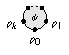
\includegraphics[width=0.25\textwidth]{figures/Fig_071_PDF157_Book145.pdf}
  \caption{浸入圆盘边界上的平行移动（原书 p.145）}
  \label{fig:brane-disk-transport}
\end{figure}
换言之，Floer 复形中的元素变成了交点处纤维之间的态射，而乘积则记录沿浸入圆盘边界的平行移动。线性映射 $\mathcal L_i(\gamma_i)$ 只依赖路径的同伦类，因此因子 $\mathcal L_0(\gamma_0)\alpha_1\mathcal L_1(\gamma_1)\cdots\alpha_k\mathcal L_k(\gamma_k)$ 在 $\psi$ 形变或退化时保持不变。这一点对 $A_\infty$ 公理中的各项相消至关重要。

在这一推广设定下，只要把 $\phi_\epsilon^h(L)$ 理解为 $(L,\mathcal L,\phi_\epsilon^h\circ\phi)$，Floer 理论的主定理仍然成立。把普通拉格朗日子流形 $L$ 视为带平凡一维局部系统的膜，就能恢复原来的 Floer 理论：对任意点 $p$ 和曲线 $\gamma$，有 $\mathcal L(p)=k$、$\mathcal L(\gamma)=1$。

局部系统的思想还可以用来描述 $L$ 上的不同自旋结构。给定 $L$ 上一个自旋结构，所有其他自旋结构可由 $H^1(L,\mathbb Z_2)$ 参数化。这个空间也可识别为所有满足如下条件的局部系统 $\mathcal S$：$\mathcal S(p)$ 为一维，且对任意闭路 $\gamma$，$\mathcal S(\gamma)=\pm1$。拉格朗日膜 $(L,\mathcal S,\phi)$ 因而可以解释为带有另一种自旋结构的同一个拉格朗日子流形。

\begin{definition}{正合 Fukaya 范畴}{exact-fukaya-category}\index{zhenghefukayafanchou@正合 Fukaya 范畴|hyperpage}
正合 Fukaya 预范畴 $\mathrm{exFuk}^\bullet(X)$ 的横截序列由两两横截相交且交点彼此不同的正合拉格朗日膜组成，乘积按上文定义。正合 Fukaya 范畴 $\mathrm{exFuk}^\bullet(X)$ 定义为相应预范畴的范畴化。
\end{definition}

\begin{example}[圆的余切丛上的局部系统与浸入]
回到带有 $\Omega=dz$ 的圆的余切丛 $T^*S^1=\mathbb C^*$。

\textbf{局部系统。} 为描述 $S^1$ 上的局部系统 $\mathcal L$，先选取基点 $b\in S^1$，并在 $\mathcal L(b)$ 中选一组基。这给出矩阵 $M=\mathcal L(\ell)$，其中 $\ell$ 是以 $b$ 为基点、沿正向绕圆一周的环路。该局部系统对应表示
\[
  \rho_M\colon\pi_1(S^1)\to\mathrm{GL}_n,
  \qquad \ell^k\longmapsto M^k.
\]
对每个其他点 $x$，从 $b$ 沿正向到 $x$ 有一条唯一的最短路径（按同伦类计）。可以选择 $\mathcal L(x)$ 中的基，使沿该路径的平行移动为恒等映射。固定这些基后，$\mathcal L(\gamma)=M^k$，其中 $k$ 是 $\gamma$ 沿正向穿过 $b$ 的次数减去沿反向穿过 $b$ 的次数。

现在考虑两个嵌入的、正合且正向定向的拉格朗日子流形 $L_1,L_2$，它们分别带有局部系统 $\mathcal L_1,\mathcal L_2$，对应矩阵为 $M_1,M_2$。若交点为 $u_i,v_i$（$1\le i\le r$），并假设两个基点都位于 $u_r$ 与 $v_1$ 之间，则 Floer 复形为
\[
  CF(L_1,L_2)=\bigoplus_{i=1}^r
  \left(\mathrm{Mat}_{n_2\times n_1}(k)u_i\oplus
        \mathrm{Mat}_{n_2\times n_1}(k)v_i\right),
\]
其中当 $i\ne r$ 时，
\[
  \mu_1(Au_i)=Av_{i+1}-Av_i,
\]
而绕过基点的最后一项为
\[
  \mu_1(Au_r)=M_2AM_1^{-1}v_1-Av_r.
\]
该复形的上同调可解释为
\[
  \operatorname{Ext}_{\pi_1(S^1)}^\bullet(\rho_{M_1},\rho_{M_2}).
\]
因此，允许局部系统后，Fukaya 范畴的行为类似于有限维 $\pi_1(S^1)$-模范畴。

\textbf{浸入。} 圆的一个浸入形如 $\phi\colon t\mapsto(kt,p(t))$，其中 $k\in\mathbb Z$ 是绕数，$p(t)$ 是 $2\pi$-周期函数。若 $p$ 是某个 $2\pi$-周期原函数 $f$ 的导数，该浸入就是正合的。

比较底圆 $L_1=S^1\subset T^*S^1$ 上由 $M_1\in\mathrm{Mat}_{2\times2}(k)$ 决定的二维局部系统，与绕圆柱两周、带有传递矩阵 $M_2\in k$ 的一维局部系统的浸入拉格朗日子流形。此时
\begin{figure}[H]\centering
  \centering
  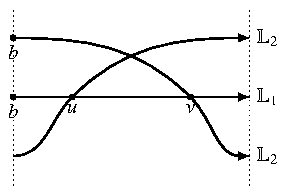
\includegraphics[width=0.54\textwidth]{figures/Fig_072_PDF159_Book147.pdf}
  \caption{嵌入圆与绕圆柱两周的浸入（原书 p.147）}
  \label{fig:immersed-circle-local-system}
\end{figure}
\[
  CF(L_1,L_2)=k^2u\oplus k^2v,
  \qquad
  \mu_1(Au)=M_1Av-M_1^{-1}AM_2^{-1}v.
\]
若 $M_1^2=M_2I_2$，该微分为零，因而有两个非零零次态射。进一步考察可知，若 $M_1=\begin{pmatrix}0&M_2\\1&0\end{pmatrix}$，则这两个对象同构。直观上，这是合理的：此时 $L_1$ 上的局部系统是沿投影 $L_2\to L_1$ 拉回 $L_2$ 上局部系统所得。

利用这一思想可以证明：任何绕圆柱 $n$ 圈、带有 $k$ 维局部系统的浸入拉格朗日子流形，都与一个嵌入拉格朗日子流形及其上的 $nk$ 维局部系统同构。

\textbf{多个连通分支。} 还可以浸入多个连通分支。此时 $L=L_1\sqcup\cdots\sqcup L_k$，浸入与局部系统在每个分支上的限制都可视为 Fukaya 范畴中的独立对象。不难证明，在加法完备化中，大对象同构于各小对象的直和：
\[
  (L,\phi,\mathcal L)\cong
  \bigoplus_i(L_i,\phi|_{L_i},\mathcal L|_{L_i}).
\]
\end{example}

从这一讨论可见，Fukaya 范畴中的对象是带局部系统的分次圆的直和。每个对象都等价于 $\pi_1(S^1)$ 或其群环 $k[X,X^{-1}]$ 上有限维模的某个移位。与多项式环的情形类似，导出范畴 $D\mathrm{mod}^\bullet k[X,X^{-1}]$ 中的每个对象都具有这种形式，因此
\[
  \mathrm{exFuk}^\bullet(X)\cong_\infty D\mathrm{mod}^\bullet k[X,X^{-1}].
\]
从这一角度看，同时纳入浸入与局部系统是很自然的。这样得到的 Fukaya 范畴性质更好，因为它对直和、移位乃至锥封闭。因此，下文所说的 Fukaya 范畴一律指这个版本，而不是最初构造的基本版本。

\subsection{wrapped Fukaya 范畴}\label{subsec:wrapped-fukaya}
在上一个例子中，我们看到，圆的余切丛的 Fukaya 范畴可以识别为 $\pi_1(S^1)$ 的有限维表示所成的 $A_\infty$ 范畴。从表示论角度看，若还能纳入一些良好的无限维模（例如有限生成投射模），会更理想。为此，我们应当在 Fukaya 范畴的构造中纳入非紧致拉格朗日子流形；显然可以选择具有锥形端的子流形。

从带柱状端、配有相容几乎复结构的 Liouville 流形 $(X,\theta,J)$ 出发。在 $X$ 上选取 Hamilton 函数 $h\colon X\to\mathbb R$，令它在 Liouville 域 $X_0$ 上为零，并在柱体的向外坐标 $r$ 上呈二次增长。该 Hamilton 函数生成的流称为 Reeb 流\index{reebliu@Reeb 流|hyperpage}，其流线
\[
  \gamma_x\colon[0,1]\to X,\qquad t\longmapsto\phi_t^h(x)
\]
称为 Reeb 弦\index{reebxian@Reeb 弦|hyperpage}。Reeb 流保持坐标 $r$ 不变，因此每条 Reeb 弦都在某个 $\partial X_0\times\{r\}$ 上绕行。随着 $r$ 增大，由于 $h$ 关于 $r$ 是二次的，Reeb 弦绕行得越来越快。

\begin{definition}{wrapped Floer 复形}{wrapped-floer-complex}
若 $L_1,L_2$ 是正合拉格朗日子流形，且 $\phi_1^hL_1$ 与 $L_2$ 横截相交，则 wrapped Floer 复形 $CW(L_1,L_2;h)$ 定义为由连接 $L_1$ 与 $L_2$ 的 Reeb 弦张成的向量空间：
\[
  CW(L_1,L_2;h)=
  \bigoplus_{\substack{\gamma(0)\in L_1\\\gamma(1)\in L_2}}k\gamma.
\]
\end{definition}

作为向量空间，该复形与 $CF^{\pm}(\phi_1^hL_1,L_2)$ 同构，因为每条 Reeb 弦都对应一个交点。利用这一识别，可以给 $CW(L_1,L_2;h)$ 赋予 $\mathbb Z_2$-分次；若 $X$ 是 Calabi--Yau 流形，还可以赋予 $\mathbb Z$-分次。
\begin{figure}[H]\centering
  \centering
  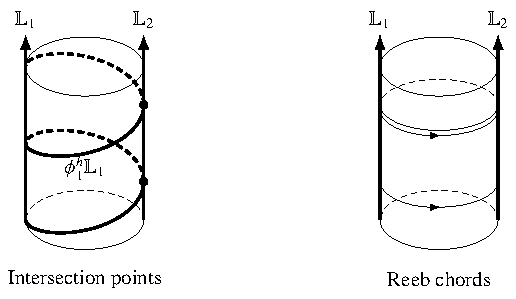
\includegraphics[width=0.79\textwidth]{figures/Fig_073_PDF161_Book149.pdf}
  \caption{交点与 Reeb 弦的对应（原书 p.149）}
  \label{fig:wrapped-intersections-chords}
\end{figure}

乘积仍通过统计浸入圆盘来定义，但此时会遇到配对问题。若 Reeb 弦 $\gamma_1$ 对应于 $\phi_1^hL_0$ 与 $L_1$ 之间的交点 $p_1$，而 Reeb 弦 $\gamma_2$ 对应于 $\phi_1^hL_1$ 与 $L_2$ 之间的交点 $p_2$，那么 $L_1$ 与 $\phi_1^hL_1$ 并不重合。可以把 $p_1$ 沿流推到交点 $\phi_1^hp_1$，它属于 $\phi_2^hL_0$ 与 $\phi_1^hL_1$ 的交点。但若以 $p_2$ 和 $\phi_1^hp_1$ 为角点统计三角形，第三个角点将落在 $\phi_2^hL_0$ 与 $L_2$ 的交点中。由于 $\phi_2^hL_0=\phi_1^{2h}L_0$，这对应于 $CW(L_0,L_2;2h)$ 中的一条 Reeb 弦。

因此，乘积 $\widetilde\mu_k$ 是映射
\[
  \widetilde\mu_k\colon
  CW(L_{k-1},L_k;h)\otimes\cdots\otimes CW(L_0,L_1;h)
  \longrightarrow CW(L_0,L_k;kh).
\]
用 Reeb 弦表述，它统计如下对象。设 $\gamma_i\in CW(L_{i-1},L_i;h)$（$i=1,\ldots,k$）是 Reeb 弦，且 $\gamma_0\in CW(L_0,L_k;kh)$。令 $D_{k+1}$ 为去掉 $k+1$ 段圆周弧后的闭单位圆盘：
\[
  D_{k+1}=D\setminus
  \bigcup_{i=0}^{k}\left\{
  e^{\frac{2t\pi i}{2k+2}}\ \middle|\ t\in(2i+1,2i+2)\right\}.
\]
考虑从 $D_{k+1}$ 到 $X$ 的映射 $\psi$，按重参数化取等价类，并要求：
\begin{itemize}
  \item 若 $t\in(2i,2i+1)$，则 $\psi(e^{\frac{2t\pi i}{2k+2}})\in L_i$；
  \item 若 $t\in(2i+1,2i+2)$、$i\in\{0,\ldots,k-1\}$，则当 $u\to e^{\frac{2t\pi i}{2k+2}}$ 时，$\psi(u)$ 的极限为 $\gamma_{i+1}(t-2i-1)$；
  \item 若 $t\in(2k+1,2k+2)$，则当 $u\to e^{\frac{2t\pi i}{2k+2}}$ 时，$\psi(u)$ 的极限为 $\gamma_0(2k+2-t)$；
  \item $\psi$ 满足一个经过变形的 Cauchy--Riemann 方程。
\end{itemize}
与原来一样，高阶乘积定义为所有不能再形变的这类映射之和。

为了得到真正的乘积，还应将 $\widetilde\mu_k$ 与映射
\[
  S_k\colon CW(L_0,L_k;kh)\to CW(L_0,L_k;h)
\]
复合。由于 $\phi_1^hL_0$ 与 $\phi_1^{kh}L_0$ Hamilton 同痕，这两个复形拟同构，所以可以选择 $S_k$ 为拟同构。要对所有可能的拉格朗日子流形自然地选取这些映射 $S_k$，并使 $\mu_k=S_k\widetilde\mu_k$ 满足 $A_\infty$ 关系，技术上相当复杂。细节可参见\bookcite{15,6}。
% [Tutor Note: 配对问题说明 $CW$ 上的乘积不能像 $CF$ 那样直接计数：$\phi_1^{kh}L_0$ 与 $\phi_1^hL_0$ 只是 Hamilton 同痕而非相等，故先用 $\widetilde\mu_k$ 落到 $CW(\cdot,\cdot;kh)$，再用拟同构 $S_k$ 拉回。原文未写出的是：这些 $S_k$ 还必须满足相干性条件（与 $\widetilde\mu$ 的复合在高阶上相容），否则 $\mu_k=S_k\widetilde\mu_k$ 不满足 $A_\infty$ 关系。]

若 $L_1,L_2$ 是包含于 Liouville 域 $X_0$ 中的紧致拉格朗日子流形，这一构造就退化为原来的构造，因为此时 $h|_{X_0}=0$，流为恒等映射。也可以像之前那样纳入浸入与局部系统。

\begin{definition}{wrapped Fukaya 范畴}{wrapped-fukaya-category}
wrapped Fukaya 预范畴 $\mathrm{wrFuk}^\bullet(X,h)$ 的对象是浸入的、正合的、带锥形端的拉格朗日子流形，其上配有自旋结构与局部系统，紧致子流形也在其中；Hom 空间是 wrapped Floer 复形 $CW^\bullet(L_0,L_1;h)$，乘积为上述 $\mu_k$。wrapped Fukaya 范畴\index{wrappedfukayafanchou@wrapped Fukaya 范畴|hyperpage} $\mathrm{wrFuk}^\bullet(X)$ 定义为该预范畴的范畴化。
\end{definition}

在 $A_\infty$ 拟等价意义下，$\mathrm{wrFuk}^\bullet(X)$ 与几乎复结构及 $h$ 的选取无关，并且有全忠实嵌入
\[
  \mathrm{exFuk}^\bullet(X)\hookrightarrow\mathrm{wrFuk}^\bullet(X).
\]

\begin{example}[圆的余切丛的 wrapped Fukaya 范畴]
回到 $T^*S^1$ 的例子。任意余切纤维 $L=T_x^*S^1$ 都是正合且带锥形端的拉格朗日子流形。每条 Reeb 弦 $\gamma$ 都由绕数 $w(\gamma)$ 决定；用 $X^{w(\gamma)}$ 表示它，就有
\[
  CW(L,L;h)\cong k[X,X^{-1}].
\]
对标准分次 $\Omega=dz/z$（取分次 $(L,\pi/2)$），所有 $X^i$ 的次数都是 $0$，所以唯一可能非零的乘积是 $\mu_2$。浸入圆盘的总绕数为零，因此非零乘积只能是
\[
  \mu(X^i,X^j)=X^{i+j}.
\]
下图在圆柱的万有覆盖上展示了相应的浸入：
\begin{figure}[H]\centering
  \centering
  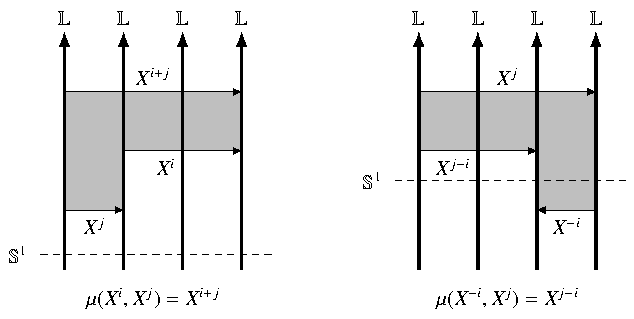
\includegraphics[width=0.88\textwidth]{figures/Fig_074_PDF163_Book151.pdf}
  \caption{$\mu(X^i,X^j)$ 与 $\mu(X^{-i},X^j)$ 的浸入圆盘（原书 p.151）}
  \label{fig:wrapped-circle-products}
\end{figure}

其他正合的锥形拉格朗日子流形可看成两条直线端由一条在底圆附近绕圆柱若干圈的曲线连接而成。若两端位于同一侧，则该对象是零对象，因为有 $1=d\gamma$，其中 $\gamma$ 是连接两端的最短 Reeb 弦。若两端位于相反侧，则该对象（取适当定向）同构于 $T^*S^1$。
\begin{figure}[H]\centering
  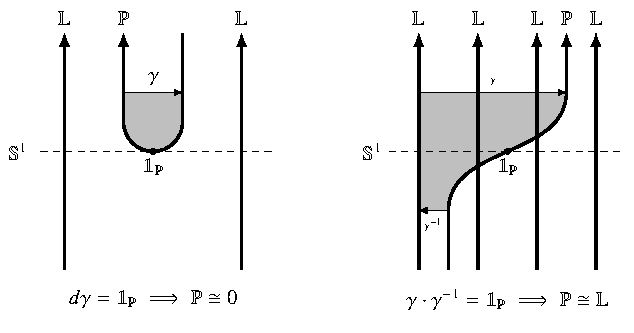
\includegraphics[width=0.79\textwidth]{figures/Fig_075_PDF163_Book151.pdf}
  \caption{由端点位置判定 wrapped 范畴中的对象（原书 p.151）}
  \label{fig:wrapped-circle-objects}
\end{figure}

因为 $L$ 可缩，其上的局部系统均为平凡局部系统；所有其他连通对象都同构于余切纤维的某个移位或直和。后者对应于自由 $k[X,X^{-1}]$-模。因此
\[
  \mathrm{wrFuk}^\bullet\left(X,\frac{dz}{z}\right)
  \cong_\infty D\mathrm{Mod}^\bullet k[X,X^{-1}].
\]
若选择分次形式 $\Omega=z^kdz$，其中 $k\ne-1$，仍可给余切纤维赋予分次，因为它是可缩的。态射 $X^i\in CW(L,L)\cong k[X,X^{-1}]$ 的次数为 $i(k+1)$。由于普通 Fukaya 范畴为空（不存在紧致对象），有
\[
  \mathrm{wrFuk}^\bullet(X,z^kdz)\cong_\infty Dk[X,X^{-1}],
  \qquad \deg X=k+1.
\]
% [Tutor Note: 原文 p.164 末作 $\deg X=k-1$，与同页上一行的“$X^i$ 的次数为 $i(k+1)$”矛盾，应为 $k+1$：由 $\Omega=z^kdz=z^{k+1}(dp+idq)$ 可见沿纤维绕行时相位按 $(k+1)$ 倍变化，故 $\deg X=k+1$。]
\end{example}

\begin{note}\label{note:wrapped-vs-ordinary-fukaya}
\textbf{观察 6.48.} wrapped Fukaya 范畴与普通 Fukaya 范畴之间的关系，类似于有限维模的导出范畴与有限生成模范畴之间的关系。
\end{note}

\subsection{partially wrapped Fukaya 范畴}\label{subsec:partially-wrapped-fukaya}
设 $(X,\theta)$ 是带柱状端的 Liouville 流形。一般而言，柱体上的 Reeb 流会使锥形拉格朗日子流形的自同态空间变成无限维。在某些情形下这是我们想要的，但另一些情形中它会带来不便。因此，我们引入一种中断该流的方法。

\begin{definition}{stop}{fukaya-stop}
设 $U_0$ 是 $\partial X_0$ 中的一个超曲面，并令 $U:=U_0\times[1,\infty)$。它构成 $X$ 的柱状端中的超曲面；若 Reeb 流处处与该超曲面法向，则称 $U$ 为 stop\index{stop@stop|hyperpage}。
\end{definition}

由于 Reeb 流处处与超曲面法向，Reeb 弦只能沿一个方向穿过它。因此，可以把 Reeb 弦的 $U$-次数定义为它穿过 $U$ 的次数。

\begin{lemma}{wrapped Fukaya 范畴中的乘积不增加 stop 次数}{stop-degree-monotonicity}
对与 $U$ 不相交的拉格朗日子流形，wrapped Fukaya 范畴中的乘积不会增加 $U$-次数。也就是说，若
\[
  \mu_k(\gamma_1,\ldots,\gamma_k)=\sum_i\alpha_i\zeta_i,
\]
则 $\zeta_i$ 的 $U$-次数至多为各 $\gamma_i$ 的 $U$-次数之和。
\end{lemma}
\begin{proof}[证明梗概]
考察由 $\gamma_i$ 围成的浸入圆盘 $\psi\colon D\to X$，其边界上还有一条输出弦 $\zeta$。原像 $\psi^{-1}(U)$ 是一族带定向曲线。这些曲线只能从 $\gamma_i$ 进入、从 $\zeta_i$ 离开，因为只有 $\zeta_i$ 在圆盘边界上的方向与之相反。
\begin{figure}[H]\centering
  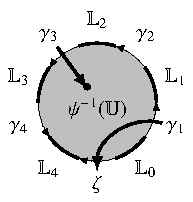
\includegraphics[width=0.44\textwidth]{figures/Fig_076_PDF165_Book153.pdf}
  \caption{圆盘中 stop 的原像曲线（原书 p.153）}
  \label{fig:stop-preimage-curves}
\end{figure}
若全纯圆盘有一部分位于柱体之外，这些曲线也可以在 $\psi^{-1}(U_0)$ 中的点处终止。
\end{proof}

\begin{definition}{partially wrapped Fukaya 范畴}{partially-wrapped-fukaya-category}
设 $\sigma$ 是一组可能彼此相交的 stop。partially wrapped Fukaya 预范畴 $\mathrm{wrFuk}^\bullet_\sigma(X)$ 的对象，是 wrapped Fukaya 范畴中与所有 $U\in\sigma$ 不相交的对象；其态射空间由 wrapped Fukaya 范畴中对每个 $U\in\sigma$ 的 $U$-次数均为 $0$ 的态射组成。partially wrapped Fukaya 范畴\index{partiallywrappedfukayafanchou@partially wrapped Fukaya 范畴|hyperpage} $\mathrm{wrFuk}^\bullet_\sigma(X)$ 定义为该预范畴的范畴化。
\end{definition}

\begin{example}[圆的余切丛上的 stop]
仍考察圆的余切空间。此时 $X_0$ 是两个圆的不交并，$U_0$ 是这些圆上的一组选定点。
% [Tutor Note: 原文 p.165 此处作“$X_0$ 是两个圆的不交并”，疑为笔误：$X_0=\{x\in T^*S^1\mid\|p\|\le1\}$ 是圆柱 $S^1\times[-1,1]$，不交并的两个圆是其边界 $\partial X_0$；紧接着的 $U_0$ 也是 $\partial X_0$ 上的点。]
每个点都会在圆柱上确定一条向外延伸的射线。这些射线把上、下两端分成不同扇区，不同扇区之间没有 Reeb 弦。
\begin{figure}[H]\centering
  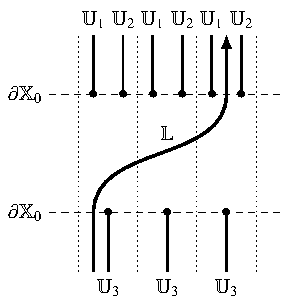
\includegraphics[width=0.86\textwidth]{figures/Fig_077_PDF165_Book153.pdf}
  \caption{圆柱端上的 stop 与扇区（原书 p.153）}
  \label{fig:stops-cylinder-sectors}
\end{figure}
锥形拉格朗日子流形由起始扇区、终止扇区及中间绕行的圈数决定。同一类型的子流形都给出同构对象。注意，在圆柱同一侧起始和终止、但处于不同扇区的对象，在 partially wrapped Fukaya 范畴中是非零对象；若移除 stop，这些对象在 fully wrapped 范畴中就变成零对象。现在考察三种特殊情形。

\begin{itemize}
  \item 若只有一个 stop（设在圆柱下端），则在同痕意义下只有一个非紧致拉格朗日子流形。它的自同态环为 $k[X]$，因为 $X$ 的所有负次幂都被 stop 消去。因此
  \[
    \mathrm{wrFuk}^\bullet_\sigma(X)\cong_\infty D\mathrm{Mod}^\bullet k[X].
  \]
  \item 若同一端有 $n$ 个 stop，则有 $n$ 条从底端通到顶端的不同拉格朗日子流形，它们的自同态环是循环箭图的路径代数。此外，对每个扇区和每个 $k$，还有一条拉格朗日子流形从顶端出发，先在 $X_0$ 中向右移动 $k$ 个扇区，再向上延伸；最后还要纳入紧致拉格朗日子流形。对照第 4.2.3 与 4.3.1 节可得
  \[
    \mathrm{wrFuk}^\bullet_\sigma(X)\cong_\infty
    D\mathrm{Mod}^\bullet\bigl(k[X]\star\mathbb Z_n\bigr).
  \]
  \item 若两端各有一个 stop，对照第 4.4.1 节可知，该范畴等价于下图所示单箭头箭图的模范畴导出范畴：
  \begin{figure}[H]\centering
    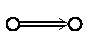
\includegraphics[width=0.13\textwidth]{figures/Fig_078_PDF166_Book154.pdf}
    \caption{单箭头箭图（原书 p.154）}
    \label{fig:single-arrow-quiver}
  \end{figure}
\end{itemize}

给定 Liouville 流形 $X$ 和一组 stop $\sigma$，由预范畴的自然嵌入给出一个 $A_\infty$ 函子
\[
  \mathrm{wrFuk}^\bullet_\sigma(X)\longrightarrow\mathrm{wrFuk}^\bullet(X).
\]
在以上每个例子中，这个函子实际上是一个局部化：一种将某个给定子范畴中的所有态射取为可逆态射的泛构造。在第一个例子中，我们把所有 $X$ 的正次幂取为可逆态射。这些态射恰好是其锥（余核）为幂零 $k[X]$-模的态射；换言之，它们是有限维 $k[[X]]$-模。因此可以写成
\[
  D\mathrm{Mod}^\bullet k[X,X^{-1}]
  \cong_\infty\frac{D\mathrm{Mod}^\bullet k[X]}{D\mathrm{mod}^\bullet k[[X]]}.
\]
partially wrapped Fukaya 范畴、移除 stop 与局部化的关系，见\bookcite{236,96}。
\end{example}

\subsection{有向 Fukaya 范畴}\label{subsec:directed-fukaya}
有向 Fukaya 范畴\index{youxiangfukayafanchou@有向 Fukaya 范畴|hyperpage}是为 Landau--Ginzburg 模型\index{landauginzburgmoxing@Landau–Ginzburg 模型|hyperpage}定义的 Fukaya 范畴。1998 年，Kontsevich 提出用这类模型研究 Fano 簇的镜像对称\bookcite{142}。其辛几何由有向 Fukaya 范畴捕捉，该范畴也称为 Fukaya--Seidel 范畴。Seidel 在其专著\bookcite{218}中详细阐述了构造；Abouzaid\bookcite{5}的工作给出略有不同的方法，并建立了它与环面 Fano 簇镜像对称之间的联系。

\begin{definition}{Landau--Ginzburg 模型}{landau-ginzburg-model}
Landau--Ginzburg 模型是一个二元组 $(X,W)$，其中 $X=(X,\theta,J)$ 是正合 Kähler 流形，$W\colon X\to\mathbb C$ 是全纯映射。
\end{definition}

可以取 $X=\mathbb C^n$，坐标 $z_i=p_i+iq_i$，并令 $\theta=p_i\,dq_i$；但更复杂的例子（例如带柱状端的 Liouville 流形）也适用。

\begin{definition}{临界点与 Lefschetz 纤维化}{lefschetz-fibration}
若在某组局部复坐标下，$W$ 的所有一阶偏导数都在 $p\in X$ 处为零，则称 $p$ 为临界点\index{linjiedian@临界点|hyperpage}。$W(p)$ 称为临界值\index{linjiezhi@临界值|hyperpage}。若 Hessian 矩阵 $\partial_{z_i}\partial_{z_j}W(p)$ 非退化，则称临界点非退化。若 $W$ 只有有限多个临界点 $\{p_1,\ldots,p_k\}$，且它们都非退化，则称 $W\colon X\to\mathbb C$ 为 Lefschetz 纤维化\index{lefschetzxianweihua@Lefschetz 纤维化|hyperpage}。
\end{definition}

Lefschetz 纤维化是 Morse 函数的复几何对应物，但二者的表现相当不同。与实情形不同，复 Hessian 总能化为单位矩阵，因此没有指标的概念。此外，Morse 函数在临界值两侧的纤维一般不同，但 Lefschetz 纤维化中所有非临界值的纤维彼此同构。
\begin{figure}[H]\centering
  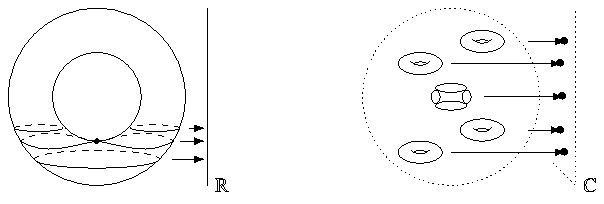
\includegraphics[width=0.38\textwidth]{figures/Fig_079_PDF167_Book155.pdf}
  \caption{Lefschetz 纤维化的正则纤维（原书 p.155）}
  \label{fig:lefschetz-regular-fibers}
\end{figure}

这是因为任意两个非临界值 $b,c$ 都可以由一条避开临界值的路径连接。取这样的路径 $\gamma\colon[0,1]\to\mathbb C$，满足 $\gamma(0)=b,\gamma(1)=c$。选择光滑函数 $h\colon\mathbb C\to\mathbb R$，令它沿 $\gamma$ 为常值、沿垂直方向变化。函数 $hW$ 在 $X$ 上生成 Hamilton 流，且 $hW$ 沿流保持不变。这意味着，投影到路径 $\gamma$ 上的点在流动后仍投影到该路径，并且该流会诱导 $W^{-1}(b)$ 与 $W^{-1}(c)$ 之间的同构。

若 $c=W(p)$ 是临界值，则 $W^{-1}(c)$ 在 $p$ 处是奇异的。前面的流构造在此失效，因为 $p$ 是流的不动点：没有点能在有限时间内到达它，但点可以渐近流向 $p$。

\begin{definition}{消失圈与 Lefschetz thimble}{vanishing-cycle-thimble}
设 $\gamma\colon[0,1]\to\mathbb C$ 是光滑嵌入，$\gamma(0)=b$ 为普通复数，$\gamma(1)=c$ 是来自临界点 $p$ 的临界值。时刻 $t\in[0,1]$ 的消失圈\index{xiaoshiquan@消失圈|hyperpage}，是纤维 $W^{-1}(\gamma(t))$ 中所有流向临界点 $p$ 的点组成的集合。Lefschetz thimble\index{lefschetzthimble@Lefschetz thimble|hyperpage}是所有这些消失圈的并：
\[
  V_{\gamma,p}(t)=\left\{x\in W^{-1}(\gamma(t))\mid
    \lim_{u\to+\infty}\phi_u^{hW}(x)=p\right\},
  \qquad
  U_{\gamma,p}=\bigcup_{t\in[0,1]}V_{\gamma,p}(t).
\]
\end{definition}
\begin{figure}[H]\centering
  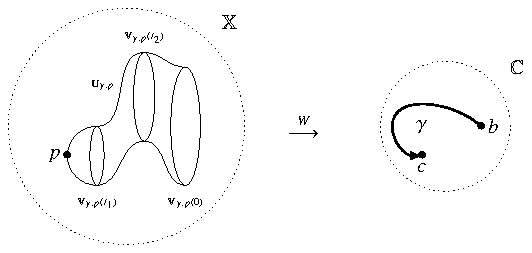
\includegraphics[width=0.66\textwidth]{figures/Fig_080_PDF168_Book156.pdf}
  \caption{消失圈与 Lefschetz thimble（原书 p.156）}
  \label{fig:vanishing-cycle-thimble}
\end{figure}

\begin{example}[二次函数的消失圈]
令 $W\colon\mathbb C^n\to\mathbb C$ 为 $W(z_i)=\sum_i z_i^2$，令 $\gamma\colon[0,1]\to D$ 为 $\gamma(t)=1-t$，并令 $h\colon\mathbb C\to\mathbb R$ 为 $h(z)=\operatorname{Im}z$。写 $z_i=q_i+ip_i$，便有 $hW=\sum_i2p_iq_i$，相应的流方程是
\[
  \dot q_i=-\frac{\partial hW}{\partial p_i}=-2q_i,
  \qquad
  \dot p_i=\frac{\partial hW}{\partial q_i}=2p_i,
\]
其解为 $(q_{0i}e^{-2t},p_{0i}e^{2t})$。流向临界点 $0$ 的点恰好满足 $p_{0i}=0$。因此
\[
  V_{\gamma,0}(t)=\left\{(\vec q,0)\mid\sum_iq_i^2=1-t\right\},
  \qquad
  U_{\gamma,0}=\left\{(\vec q,0)\mid\sum_iq_i^2\le1\right\}.
\]
在 $t=0$ 时，消失圈是超曲面 $\sum_i z_i^2=1$ 中的一个拉格朗日球面，而 thimble 是 $\mathbb C^n$ 中的实球。若换用另一个函数，例如 $h=g\,\operatorname{Im}z$（其中 $g\colon\mathbb C\to\mathbb R$），流方程变为
\[
  \dot q_i=-2q_i\left(g+p_i\frac{\partial gW}{\partial p_i}\right),
  \qquad
  \dot p_i=2p_i\left(g+q_i\frac{\partial gW}{\partial q_i}\right).
\]
方程的精确解会改变，但若 $p_i=0$，它仍保持为零，因此消失圈和 thimble 不变。
\end{example}

\begin{lemma}{消失圈与 Lefschetz thimble 的性质}{vanishing-cycle-exactness}
消失圈与 Lefschetz thimble 分别是 $W^{-1}(\gamma(t))$ 与 $\mathbb C^n$ 中的正合拉格朗日子流形。它们只依赖于 $\gamma$ 和 $W$，而不依赖于 $h$。
\end{lemma}
\begin{proof}[证明梗概]
可以在局部处理这个问题，之后便归结为上面的计算。
\end{proof}

现在假设所有临界值都位于圆盘 $D\subset\mathbb C$ 内，并在圆盘边界上选取基点 $b$。给定从基点到某个临界值的曲线 $\gamma\colon b\to c$ 和临界点 $p\in W^{-1}(c)$，就可以构造消失圈和 thimble。即使流向同一个临界点，不同曲线也会给出不同 thimble。为了研究这些 thimble，我们希望把它们组织成一个范畴。

\begin{definition}{有向 Fukaya 范畴}{directed-fukaya-category}
有向 Fukaya 预范畴 $\mathrm{drFuk}^\bullet(X,W)$ 的对象是所有 Lefschetz thimble $U_{\gamma,p}$，其中 $\gamma\colon[0,1]\to D$ 是从基点 $b$ 到任一临界值 $c=W(p)\in D$ 的曲线，并且 $\gamma$ 在 $b$ 处的切向量指向圆盘内部。给这些 thimble 赋予定向、自旋结构和局部系统。

对象序列 $(U_{\gamma_1,p_1},\ldots,U_{\gamma_k,p_k})$ 称为横截的，若 thimble 两两横截相交，且切向量 $\dot\gamma_1(0),\ldots,\dot\gamma_k(0)$ 的辐角依次递增。换言之，沿基点 $b$ 附近的小圆逆时针行走，进入 $D$ 后会依次遇到 $\gamma_1,\gamma_2$ 等曲线。有向 Fukaya 预范畴的 Hom 空间和乘积按通常方式定义。有向 Fukaya 范畴 $\mathrm{drFuk}^\bullet(X,W)$ 是其范畴化。
\end{definition}
\begin{figure}[H]\centering
  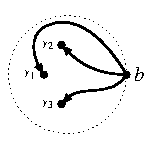
\includegraphics[width=0.26\textwidth]{figures/Fig_081_PDF169_Book157.pdf}
  \caption{基点处有序排列的消失路径（原书 p.157）}
  \label{fig:directed-vanishing-paths}
\end{figure}

\begin{note}\label{note:directed-fukaya-basepoint}
\textbf{注 6.59.} 有向 Fukaya 范畴的定义依赖于边界基点（以及圆盘的大小），但不同选择给出等价范畴，因为可以找到一个旋转边界、但固定临界点的流。这个流会在不同基点对应的有向 Fukaya 范畴之间诱导等价。
\end{note}

\begin{example}[圆环上的 Landau--Ginzburg 模型]\label{ex:punctured-plane-lg-model}
令 $X=\mathbb C^*$，并定义 $W\colon\mathbb C^*\to\mathbb C$，$W(z)=\frac{z-z^{-1}}{4}$。临界点为 $p_\pm=\pm i$，临界值为 $\pm\frac{i}{2}$。取基点 $b=1$，则
\[
  W^{-1}(b)=\left\{x_+,x_-\right\},
  \qquad x_\pm=2\pm\sqrt5.
\]
任取曲线 $\gamma\colon1\to a$，沿 $W$ 提升可得到两条曲线
\[
  \gamma_\pm=2\gamma\pm\sqrt{4\gamma^2+1}.
\]
时刻 $t$ 的消失圈为 $\{\gamma_+(t),\gamma_-(t)\}$，Lefschetz thimble 则是这两条曲线的并。下图展示三个例子和对应的基圆盘路径：
\begin{figure}[H]\centering
  \centering
  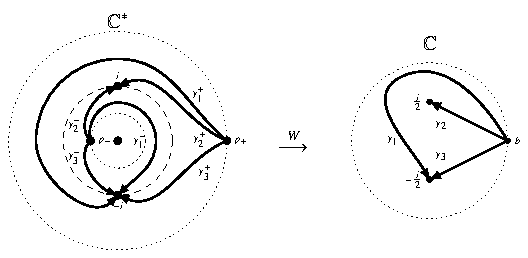
\includegraphics[width=0.74\textwidth]{figures/Fig_082_PDF170_Book158.pdf}\quad
  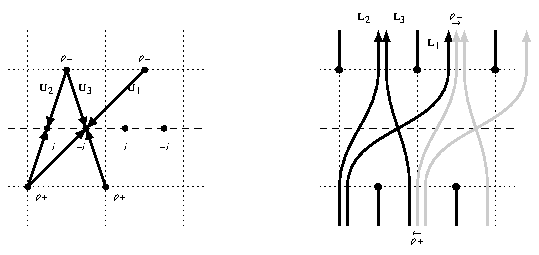
\includegraphics[width=0.53\textwidth]{figures/Fig_083_PDF170_Book158.pdf}
  \caption{圆环上的消失路径及其提升（原书 p.158）}
  \label{fig:punctured-plane-thimbles}
\end{figure}
由于没有浸入圆盘，态射空间为
\[
  \begin{aligned}
  \mathrm{drFuk}^\bullet(U_1,U_2)&=kp_+\oplus kp_-,\\
  \mathrm{drFuk}^\bullet(U_2,U_3)&=kp_+\oplus kp_-,\\
  \mathrm{drFuk}^\bullet(U_1,U_3)&=kp_+\oplus kp_-\oplus kc,
  \end{aligned}
\]
其中 $c$ 表示点 $-i$。

把圆柱展开后，可以看到这一例子与圆的余切丛上、两端各有一个 stop 的 partially wrapped Fukaya 范畴惊人地相似。若在 $p_+$ 与 $p_-$ 附近放置 stop，并把 thimble 两端都延伸到无穷远处，就得到 partially wrapped 范畴中的对象，其态射空间恰好相同。再做一些工作，可以构造函子
\[
  \mathrm{drFuk}^\bullet(\mathbb C^*,W)
  \longrightarrow\mathrm{wrFuk}^\bullet_\sigma(\mathbb C^*),
\]
它在转到导出范畴后成为等价。这一例子说明，在许多情形中，partially wrapped Fukaya 范畴与有向 Fukaya 范畴可以看作同一枚硬币的两面。
\end{example}

\subsection{相对 Fukaya 范畴}\label{subsec:relative-fukaya}
到目前为止所考虑的设定，都是辛流形非紧致的情形。这是因为我们只处理了正合辛流形。

\begin{lemma}{正合辛流形不能紧致}{exact-symplectic-noncompact}
正合辛流形不可能是紧致的。
\end{lemma}
\begin{proof}[证明梗概]
若 $(X,\omega)$ 是 $2n$ 维辛流形，则 $\omega^n$ 是 $X$ 上的体积形式。若 $\omega=d\theta$，则 $\omega$ 的上同调类为零，因而 $\omega^n$ 的上同调类也为零；这不可能，因为体积形式在紧致定向流形上的积分非零。
\end{proof}

为紧致流形定义 Fukaya 范畴颇为困难，因此我们先构造一个中间版本。Seidel 在\bookcite{217}中引入了这一构造。设 $X$ 是紧致 Kähler 流形，且
\[
  D=\bigcup_{i\in I}D_i
\]
是若干光滑、彼此横截相交的复超曲面的并，并假设 $X\setminus D$ 是带柱状端的 Liouville 流形。于是可以按通常方式定义 $X\setminus D$ 上的 Fukaya 范畴。

若把 $D$ 加回去，会发生什么？$\mathrm{exFuk}^\bullet(X\setminus D)$ 中的每个对象也可看成 $X$ 中的拉格朗日膜，且这些对象之间的交点在 $X$ 与 $X\setminus D$ 中相同。但乘积不同：在 $X$ 中可能出现额外的伪全纯圆盘，它们与除子相交，甚至可能有无穷多个。

为了记录这些圆盘，我们考虑由各 $D_i$ 自由生成的幺半群 $G$，并取其形式幂级数环 $k[[G]]$。利用第 3.4.3 节所述技术，应当可以把正合 Fukaya 范畴 $\mathrm{exFuk}^\bullet(X\setminus D)$ 变形为一个带曲率的 $G$-滤过 $A_\infty$ 范畴 $\mathrm{cuFuk}^\bullet(X,D)$，使得对每个
\[
  g=g_1D_1+\cdots+g_kD_k,
\]
都有
\[
  \mu_{k,g}(p_1,\ldots,p_k)=\sum_{p_0}\sum_\psi\sigma_\psi p_0,
\]
其中 $\psi$ 遍历所有与每个 $D_i$ 的交数为 $g_i$ 的全纯映射。要使这一构造成立，还需处理一些问题：
\begin{itemize}
  \item 对每种交数，圆盘的数目都必须有限；
  \item 可能发生圆盘起泡，从而产生 $\mu_0$；
  \item 可能发生球面起泡，球面甚至可能完全包含在某个除子中，因而导致负交数。
\end{itemize}
为解决这些问题，必须限制允许的除子类型，而且可能需要在更大的系数环上工作。更多细节见\bookcite{217,224}。目前，完全一般的构造仍在发展中；不过，概念上的思路如下。

\begin{definition}{相对 Fukaya 范畴}{relative-fukaya-category}
相对 Fukaya 范畴\index{xiangduifukayafanchou@相对 Fukaya 范畴|hyperpage} $\mathrm{cuFuk}^\bullet(X,D)$ 是正合 Fukaya 范畴 $\mathrm{exFuk}^\bullet(X\setminus D)$ 的一个带曲率变形；其乘积按照全纯圆盘与 $D$ 的交型计数。
\end{definition}

\begin{note}\label{note:relative-fukaya-parameter}
\textbf{注 6.63.} 对上述方案的一个重要变体是：不把 $D$ 看成分量 $D_i$ 的并，而是把它视为带自然数系数的线性组合 $D=\sum_i a_iD_i$。这确定一个映射
\[
  k[[G]]\to k[[\hbar]],\qquad
  \hbar^{D_i}\longmapsto\hbar^{a_i},
\]
从而可以把相对 Fukaya 范畴看成定义在 $k[[\hbar]]$ 上的变形，而非定义在 $k[[G]]$ 上。
\end{note}

\begin{note}\label{note:uncurving-relative-fukaya}
\textbf{注 6.64.} 把这个带曲率范畴转化为无曲率范畴有多种方法。最简单的是取带曲率的扭曲复形，并考察满足曲率 $\widehat\mu_0=\lambda1$（其中 $\lambda\in k[[G]]$ 或 $k[[\hbar]]$）的对象所成子范畴。忘掉 $\widehat\mu_0$ 后，这便是一个无曲率滤过范畴，记为 $\lambda\mathrm{Fuk}^{\pm}(X,D)$。若 $X$ 是 Calabi--Yau 流形，可以给 Fukaya 范畴赋予 $\mathbb Z$-分次；此时 $\lambda$ 的次数必须为 $2$，所以只能有 $\lambda=0$。在这种情形下，省略前缀并记作 $\mathrm{Fuk}^\bullet(X,D)$。这些范畴定义在 $k[[G]]$ 上，而 $k[[G]]$ 不是域，因此取极小模型时必须谨慎。

可以沿用第 3.4.3 节的策略，把范畴与 $k((G))$ 作张量，从而得到域上的 $A_\infty$ 范畴并取其极小模型。所得范畴记作
\[
  \lambda D\mathrm{Fuk}^{\pm}(X,D)\otimes k((G))
  \quad\text{或}\quad
  D\mathrm{Fuk}^\bullet(X,D)\otimes k((G)).
\]

有时，$\mathrm{cuFuk}^{\pm}(X,D)$ 中的乘积 $\widehat\mu_k$ 并非形式幂级数，而是实际的多项式。此时，可以通过选取映射 $\rho\colon G\to\mathbb C$，将这些多项式特化为复数。若此外当 $k$ 足够大时 $\widehat\mu_k=0$，就考察满足 $\rho(\widehat\mu_0)=\lambda1$（$\lambda\in\mathbb C$）的扭曲复形；这会给出定义在 $\mathbb C$ 上的无曲率 $A_\infty$ 范畴。
\end{note}

\begin{example}[球面上的相对 Fukaya 范畴]
令 $X$ 为 Riemann 球面，取除子 $D=\{0\}+\{\infty\}$。于是 $X\setminus D=\mathbb C^*=T^*S^1$，系数环取 $k[[\hbar]]$。相对 Fukaya 范畴是
\[
  \mathrm{exFuk}^{\pm}(\mathbb C^*)
  \cong_\infty D\mathrm{mod}^{\pm}\mathbb C[X,X^{-1}]
\]
的一个变形。注意，这只能是 $\mathbb Z_2$-分次变形，因为体积形式 $dz/z$ 不能延拓到 Riemann 球面。

若 $(L,\rho_M)$ 是底圆，且局部系统的平行移动由 $M\in\mathbb C^*$ 给出，那么有两个以 $S^1$ 为边界的全纯圆盘：球面的上半部和下半部。它们分别穿过 $0$ 与 $\infty$；边界定向相反，因此沿圆的平行移动互为逆。把所有 $\mu_0$ 乘积合起来，得到
\[
  \widehat\mu_0\big|_{(L,\rho_M)}
  =(M\hbar+M^{-1}\hbar)\,\iota.
\]
\begin{figure}[H]\centering
  \centering
  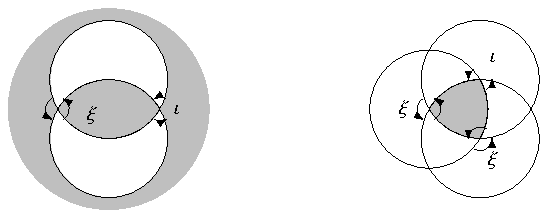
\includegraphics[width=0.73\textwidth]{figures/Fig_084_PDF173_Book161.pdf}
  \caption{穿过除子两分支的圆盘（原书 p.161）}
  \label{fig:relative-fukaya-sphere-disks}
\end{figure}

为了确定 $(L,\rho_M)$ 的自同态之间的乘积，我们考察一列与圆同痕的拉格朗日子流形。对一元乘积有两个圆盘贡献；其他乘积各只有一个贡献，因为另一个圆盘会多次绕过 $\infty$，不再是浸入。于是
\[
  \widehat\mu_1(\xi)=(M\hbar-M^{-1}\hbar)\,\iota,
  \qquad
  \widehat\mu_k(\xi,\ldots,\xi)=M\hbar\,\iota\quad(k\ge2).
\]
因此，除非 $M=\pm1$，对象 $(L,\rho_M)$ 都是零对象。把剩下两个对象记为 $L_\pm$。它们是曲率分别为 $\pm2\hbar$ 的带曲率对象，但可以视为无曲率范畴
$\pm2\hbar\,\mathrm{Fuk}^{\pm}(X,D)\otimes k((\hbar))$ 中的对象。经过一次 $A_\infty$ 同构，可以令 $\widehat\mu_{\ge3}=0$，因此这两个对象的自同态环为
\[
  \frac{k((\hbar))[\xi]}{(\xi^2\pm\hbar)}.
\]
\end{example}

\subsection{完整 Fukaya 范畴}\label{subsec:full-fukaya}
我们已经走到旅程的最后阶段：完整 Fukaya 范畴。给定紧致 Kähler 流形 $(X,\omega,J)$，该范畴应纳入所有拉格朗日膜。如前所述，非正合性意味着圆盘的辛面积没有上界，因此不能直接应用 Gromov 紧致性定理来证明给定一组拉格朗日子流形边界时全纯多边形只有有限多个。因此，乘积可能包含无穷多项，甚至未必定义良好。

尽管如此，对任意给定上界，面积低于该上界的全纯多边形仍然只有有限多个。因此，一般而言，乘积会是按面积递增排列的项所组成的级数。于是可以在滤过设定下工作。令 $G\subset\mathbb R_{\ge0}$ 为所有可能出现的全纯圆盘面积生成的幺半群。环 $k[[G]]$ 可视为 Novikov 域\index{novikovyu@Novikov 域|hyperpage}的子环；Novikov 域由实指数递增的幂级数构成：
\[
  V=\left\{\sum_{i=0}^{\infty}\lambda_iT^{r_i}\ \middle|\ 
  \lambda_i\in k,\ r_i\in\mathbb R,\ i>j\Rightarrow r_i>r_j\right\}.
\]

要从这里得到定义良好的范畴仍很技术性，并且需要限制允许的流形类型（例如无环流形，或满足 $\langle\pi_2(X),\omega\rangle=0$ 的流形）和膜类型（例如单调膜）。考虑这些限制后，便得到完整 Fukaya 范畴。其构造和技术细节超出本书范围，更多信息可参阅专著\bookcite{83,84}。

在理想情形下，我们得到一个 $G$-滤过的带曲率 $A_\infty$ 范畴 $\mathrm{cuFuk}^{\pm}_V(X)$，其对象是带有 $U_n$-局部系统的紧致拉格朗日膜。对任意 $\lambda\in V$，曲率为 $\lambda$ 的带曲率扭曲对象构成 Novikov 域上的普通 $A_\infty$ 范畴 $\lambda\mathrm{Fuk}^{\pm}_V(X)$。

\begin{note}\label{note:unitary-local-systems}
\textbf{注 6.66.} 这里只使用 $U_n$-局部系统，而不使用 $\mathrm{GL}_n$-局部系统，是因为局部系统的实部可以吸收到拉格朗日子流形的位置中。例如，对 $T^*S^1=\mathbb C^*$，带有实局部系统的底圆 $\{|z|=1\}$ 可解释为移位后的圆 $\{|z|=r\}$ 配上平凡局部系统。注意，后者不是正合拉格朗日子流形，因此不属于 $\mathrm{exFuk}^\bullet(\mathbb C^*)$，但它是完整 Fukaya 范畴 $\mathrm{Fuk}^\bullet_V(\mathbb C^*)$ 的对象。
\end{note}

\begin{example}[环面上的 theta 函数]
令 $T=\mathbb C/(\mathbb Z+i\mathbb Z)$ 为带标准辛结构的环面，坐标为 $z=q+ip$，辛形式为 $\omega=a\,dp\wedge dq$。考察 Fukaya 范畴中的三个对象 $L_0,L_1,L_2$，分别对应方程
\[
  q=0,\qquad p=0,\qquad p+q=\frac12.
\]
三个交点为
\[
  p_1=(0,0)\in L_0\cap L_1,\quad
  p_2=(\tfrac12,0)\in L_1\cap L_2,\quad
  p_0=(0,\tfrac12)\in L_0\cap L_2.
\]
为了求乘积 $\mu(p_2,p_1)$，要统计以 $p_0,p_1,p_2$ 为角点的浸入三角形。在万有覆盖上，这些三角形都是等腰直角三角形。固定 $p_1$ 后，三角形由一条边的长度及其定向唯一确定；边长是奇数个半单位，即 $(2k+1)/2$，相应面积为 $\frac a8(2k+1)^2$。所得幂级数可以用 Jacobi theta 函数 $\vartheta_2(z,t)$ 整齐地表示：
\begin{figure}[H]\centering
  \centering
  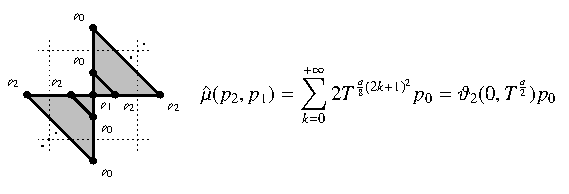
\includegraphics[width=0.72\textwidth]{figures/Fig_085_PDF174_Book162.pdf}
  \caption{环面上三角形的计数与 theta 函数（原书 p.162）}
  \label{fig:torus-triangles-theta}
\end{figure}
\[
  \widehat\mu(p_2,p_1)=
  \sum_{k=0}^{+\infty}2T^{\frac a8(2k+1)^2}p_0
  =\vartheta_2(0,T^{a/2})p_0.
\]
\end{example}

\subsection{联系}\label{subsec:fukaya-connections}
设 $(X,\omega,J)$ 是 Kähler 流形，$D$ 是使得 $\breve X:=X\setminus D$ 成为 Liouville 流形的除子，并设 $W\colon\breve X\to\mathbb C$ 是全纯函数。在理想情形下，可以找到一组 stop $\sigma$，阻断 thimble 锥形端不同部分之间的所有 Reeb 弦。此时会得到如下 $A_\infty$ 范畴关系图：
\begin{figure}[H]\centering
  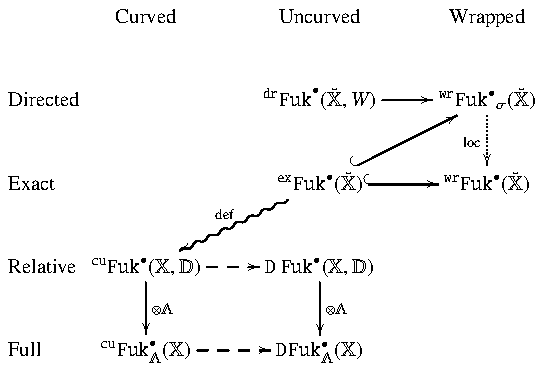
\includegraphics[width=0.86\textwidth]{figures/Fig_086_PDF175_Book163.pdf}
  \caption{$A_\infty$ 范畴之间的联系（原书 p.163）}
  \label{fig:fukaya-category-connections}
\end{figure}
蛇形箭头表示变形，点线箭头表示局部化，虚线箭头表示取无曲率扭曲复形。指向最下行的箭头表示先改变底环，再作嵌入。

\section{生成元}\label{sec:fukaya-generators}
前面已经看到，定义 Fukaya 范畴时有许多不同选择：可以纳入或排除不同类型的对象，也可以允许或禁止某些态射。这些选择会产生彼此相关但并不相同的范畴。转向导出范畴或分裂导出范畴，可以解决其中一部分问题；从表示论的角度看，这样便把本应属于范畴的对象都纳入进来。

这种做法往往也使范畴更容易描述：我们可以寻找一组生成元，并尝试把整个范畴看成少数对象的扭曲完备化。相比整个范畴，此时只需描述这些对象之间的部分或全部态射乘积，便能相当细致地刻画分裂导出 Fukaya 范畴。

\takeaway{次数为 $1$ 的态射 $x\colon L_1\to L_2$ 给出拉格朗日手术 $L_1+_xL_2\cong\operatorname{Cone}(x)$，这是用锥判定生成的基本手段；由此可知余切丛由单个余切纤维生成、曲面上的弧系生成 wrapped Fukaya 范畴，Abouzaid 判据则用开闭映射检测生成性。}

\subsection{Fukaya 范畴中的锥}\label{subsec:fukaya-cones}
要理解几何上何谓生成 Fukaya 范畴，先要考察锥构造。设两个拉格朗日子流形 $L_1,L_2$ 在一点 $x$ 横截相交。在 $x$ 的邻域内可取典范坐标 $p_i,q_i$，使得 $L_1$ 由方程 $p_i=0$ 给出，$L_2$ 由方程 $q_i=0$ 给出。

\begin{figure}[H]\centering
  \centering
  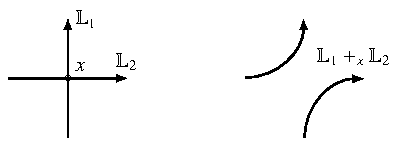
\includegraphics[width=0.72\textwidth]{figures/Fig_087_PDF176_Book164.pdf}
  \caption{横截交点处的拉格朗日手术（原书 p.164）}
  \label{fig:lagrangian-surgery-cone}
\end{figure}

对任意 $\varepsilon>0$，由方程 $p_iq_i+\varepsilon=0$ 定义的子流形 $L_\varepsilon$ 是拉格朗日子流形；不同 $\varepsilon$ 对应的子流形之间存在 Hamilton 同伦，其生成函数在 $L_\varepsilon$ 邻域内为 $f=\sum_i\log(p_iq_i)$。我们可以构造一个拉格朗日子流形 $L_1+_xL_2$：它在 $x$ 附近的开球内与 $L_\varepsilon$ 相同，在稍大的开球之外与 $L_1\cup L_2$ 相同；在两个球之间稍作调整，使两部分平滑接合。对任意交点 $x$ 都可以这样做；不过，若要使定向相容，还需要交点 $x$ 的 $\mathbb Z_2$ 次数为 $1$。

\begin{theorem}{拉格朗日手术与锥}{lagrangian-surgery-is-cone}
对象 $L_1+_xL_2$ 同构于 $\operatorname{Cone}(x)$，其中 $x$ 被视为次数为 $1$ 的态射 $x\colon L_1\to L_2$。
\end{theorem}
\begin{proof}[证明思路]
取任意一个与 $L_1+_xL_2$ 横截相交、且不进入我们作粘接的 $x$ 邻域开球的拉格朗日子流形 $U$。由于每个交点都落在 $L_1$ 或 $L_2$ 上，Floer 复形分解为
\[
  CF(L_1+_xL_2,U)=CF(L_1,U)\oplus CF(L_2,U).
\]
若有一个全纯 $n$ 边形，其一条边界落在 $L_1+_xL_2$ 上，就令 $\varepsilon\to0$ 对它作退化。所得全纯圆盘的边界落在 $L_1\cup L_2$ 上，可能完全位于 $L_1$ 上、完全位于 $L_2$ 上，或同时经过二者。前两种情形下，$n$ 边形仍是 $n$ 边形；第三种情形下，它变成一个多出角点 $x$ 的 $(n+1)$ 边形。因此，凡是含有 $L_1+_xL_2$ 的 $(n-1)$ 元乘积，都等于通常的 $(n-1)$ 元乘积与插入一个额外 $x$ 的 $n$ 元乘积之和。这正是锥构造中的乘积规则。
\end{proof}

\begin{note}\label{note:cone-multiple-intersections}
\textbf{注 6.69.} 若 $L_1$ 与 $L_2$ 有多个交点，那么 $L_1+_xL_2$ 通常不是嵌入的拉格朗日子流形，而是一个浸入。另一种可能是 $L_1+_xL_2$ 由多个连通分支组成；此时应把每个分支看作 $\operatorname{Cone}(x)$ 的一个直和项。
\end{note}

\begin{note}\label{note:cone-extensions}
\textbf{注 6.70.} 这个构造有若干推广。
\begin{itemize}
  \item 若 $L_1,L_2$ 带有局部系统，且态射为 $\alpha x$，其中 $\alpha\colon L_1(x)\to L_2(x)$ 是可逆线性映射，则可以在 $L_1+_xL_2$ 上定义新的局部系统。先在 $L_1+_xL_2$ 的每个连通分支上选取一个基点，要求在退化到 $L_1\cup L_2$ 时该基点不趋于 $x$。基点处的每条闭路在退化后成为 $L_1\cup L_2$ 上的一条折线路径，其各段分别落在 $L_1$ 或 $L_2$ 上，并在 $x$ 处衔接。沿各段使用原有局部系统的线性映射；每次从 $L_1$ 转到 $L_2$ 时插入 $\alpha$，反向转接时插入 $\alpha^{-1}$，便得到所需的整体映射。
  \item 若 $L_1,L_2$ 在多个点 $x_1,\ldots,x_k$ 相交，则可把 $\alpha_1x_1+\cdots+\alpha_kx_k$ 的锥理解为同时在这些交点处作手术得到的新拉格朗日子流形。
\end{itemize}
\end{note}

\subsection{余切丛的生成元}\label{subsec:cotangent-generators}
考察圆柱 $X=T^*S^1=\mathbb C^*$，并赋予它标准体积形式 $dz$。我们曾得到如下包含链：
\[
  \mathrm{Fuk}^{\mathrm{ba}}X\subset \mathrm{Fuk}^{\mathrm{ex}}X\subset \mathrm{Fuk}^{\mathrm{wr}}X.
\]
第一个范畴在移位意义下只有一个对象 $L_1$，其自同态环为 $k[\xi]/(\xi^2)$。在第二个范畴中，每个不可分解对象在移位意义下都对应一个圆及其上的局部系统 $\rho$。第三个范畴还包含非紧拉格朗日子流形，例如余切纤维 $U=T_x^*S^1$。

余切纤维的自同态环为 $k[X,X^{-1}]\cong k[\pi_1(S^1)]$，并且它生成 $\mathrm{Fuk}^{\mathrm{wr}}X$。事实上，任意非紧拉格朗日子流形都同构于 $U$ 的某个移位。若 $L$ 是带有局部系统 $\rho\colon\pi_1(S^1)\to\mathrm{GL}_n$ 的圆，则可将 $L$ 识别为 $\operatorname{Cone}(f)$，其中 $f=(1+\rho(\ell))1_n$ 是从 $U^{\oplus n}$ 到 $U[-1]^{\oplus n}$ 的次数 $1$ 态射，$\ell$ 是圆周基本群的生成元。

几何上，取 $1+\rho(\ell)X$ 的锥，会在两点处把 $\phi_1^h(U)$ 与 $U$ 粘接起来，得到三条曲线：一条闭曲线和圆柱两端各一条开曲线。后两条是零对象；闭曲线则是带有局部系统的紧致拉格朗日子流形。沿圆周的平行移动恰为 $\rho(\ell)$，因为在一处用恒等矩阵粘接纤维，在另一处则用 $\rho(\ell)$ 粘接。

\begin{figure}[H]\centering
  \centering
  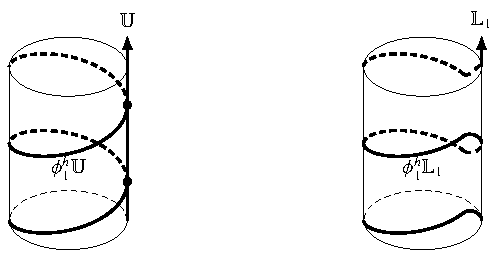
\includegraphics[width=0.76\textwidth]{figures/Fig_088_PDF178_Book166.pdf}
  \caption{圆柱上由余切纤维构造锥（原书 p.166）}
  \label{fig:cylinder-cotangent-cone}
\end{figure}

对于正合 Fukaya 范畴，情形有所不同。由于其中没有这些非紧对象，不存在有限生成集。要生成所有可能的局部系统，就需要对 $\rho(\ell)$ 的每个可能特征值各取一个生成元。因此，分裂导出正合 Fukaya 范畴由所有 $L_\lambda$ 生成，其中 $L_\lambda$ 是带一维局部系统、且 $\rho(\ell)=\lambda$ 的圆。它们之中只有 $L_1$ 属于基本 Fukaya 范畴，并生成该范畴：
\[
  D^\pi\mathrm{Fuk}^{\mathrm{ba}}X\simeq\langle L_1\rangle
  \subset D^\pi\mathrm{Fuk}^{\mathrm{ex}}X=\langle L_\lambda\mid\lambda\in k^*\rangle
  \subset D^\pi\mathrm{Fuk}^{\mathrm{wr}}X=\langle U\rangle.
\]
Abouzaid 对圆柱上 wrapped Fukaya 范畴的生成结论可以推广到所有余切丛；详细论证见文献\bookcite{7}。

\begin{theorem}{Abouzaid 生成定理}{abouzaid-cotangent-generation}
设 $M$ 是紧致连通黎曼流形。余切丛 $X=T^*M$ 的 wrapped Fukaya 范畴由一个余切纤维生成：
\[
  D^\pi\mathrm{Fuk}^{\mathrm{wr}}T^*M=\langle T_x^*M\rangle.
\]
\end{theorem}
\begin{proof}[证明思路]
首先，所有余切纤维彼此同构。由 $x$ 到 $y$ 的测地线给出 $T_x^*M$ 与 $T_y^*M$ 之间的一条 Reeb 弦；它是可逆态射，因为其逆对应于沿同一测地线反向行进。

现在取一个与零截面 $M$ 横截相交的拉格朗日子流形 $L$。选取函数 $f\colon M\to\mathbb R$，使其零点恰为交点，并考察流像 $\phi_f^tL$。当 $t\to\infty$ 时，这个流像趋于位于这些交点处的余切纤维之并。因此，$\phi_f^tL$ 可以看成这些余切纤维之间某个态射的锥。具体而言，该态射是若干 Reeb 弦之和；相对于余切纤维，这些 Reeb 弦同伦于连接交点的曲线。

\begin{figure}[H]\centering
  \centering
  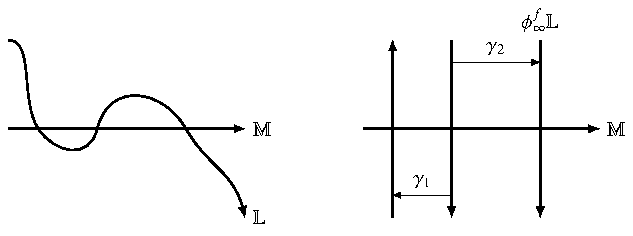
\includegraphics[width=0.76\textwidth]{figures/Fig_089_PDF179_Book167.pdf}
  \caption{拉格朗日子流形流向余切纤维之并（原书 p.167）}
  \label{fig:cotangent-flow-limit}
\end{figure}
\end{proof}

\begin{corollary}{Abouzaid}{abouzaid-loop-space}
余切丛的 wrapped Fukaya 范畴与环路空间上同调环的导出范畴分裂导出等价：
\[
  D^\pi\mathrm{Fuk}^{\mathrm{wr}}T^*M\simeq D^\pi H^\bullet(\mathcal L_xM).
\]
\end{corollary}
\begin{proof}[证明思路]\par
从 $T_x^*M$ 到自身的 Reeb 弦构成环路空间上某个 Morse 函数的临界点。因此，$\mathrm{Fuk}^{\mathrm{wr}}(T_x^*M,\allowbreak T_x^*M)$ 可以解释为环路空间上同调的一种模型。
\end{proof}

\subsection{有向 Fukaya 范畴的生成元}\label{subsec:directed-generators}
对于有向 Fukaya 范畴，可以构造许多生成集。设 $W\colon X\to\mathbb C$ 是 Lefschetz 纤维化，有 $k$ 个不同临界点 $p_i$，对应临界值 $c_i=W(p_i)$，且这些临界值彼此不同。选取 $k$ 条曲线 $\gamma_i$，使每条曲线都从基点 $b$ 出发，分别通向一个临界值；再假设这些曲线从 $b$ 出发的方向互不相同，且仅在 $b$ 相交。这样的曲线系称为一个例外序列\index{liewaixulie@例外序列|hyperpage}。

\begin{theorem}{Seidel 生成定理}{seidel-directed-generation}
例外序列对应的 thimble 生成有向 Fukaya 范畴：
\[
  D^\pi\mathrm{Fuk}^{\mathrm{dr}}(X,W)=\langle U_{\gamma_i}\mid i=1,\ldots,k\rangle.
\]
\end{theorem}
\begin{proof}[证明思路]
每条从 $b$ 到某临界值的互不相交曲线都可以扩充为一个例外序列。可以证明，任意两个例外序列都能通过称为变异的过程互相转换：取基点处相邻的两条曲线，在其中一条上添加绕另一条一周的环路，从而交换它们的次序。

可以证明，变异后新得到的 thimble 可由原 thimble 取锥表示，反过来也成立。因此，两组 thimble 生成同一个范畴。由于每个 thimble 都能出现在某个例外序列中，每个例外序列都生成全部 thimble。
\end{proof}

\begin{example}[圆柱上的 Lefschetz 纤维化]\label{ex:lefschetz-cylinder-quiver}
例~\ref{ex:punctured-plane-lg-model} 中考察了 Lefschetz 纤维化 $\pi\colon\mathbb C^*\to\mathbb C$，$z\mapsto\frac{z-z^{-1}}{4}$。它有两个临界点，临界值为 $\pm\frac{i}{2}$。我们考虑了三条曲线 $\gamma_1,\gamma_2,\gamma_3$；其中 $\gamma_1,\gamma_2$ 构成一个例外序列，$\gamma_2,\gamma_3$ 也构成一个例外序列。前者是后者的一次变异。两种情况下，自同态环都是二顶点双箭图的路径代数。因此
\begin{figure}[H]\centering
  \centering
  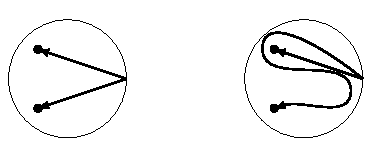
\includegraphics[width=0.48\textwidth]{figures/Fig_090_PDF180_Book168.pdf}
  \caption{例外序列的变异（原书 p.168）}
  \label{fig:mutation-two-curves}
\end{figure}
\begin{figure}[H]\centering
  \centering
  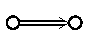
\includegraphics[width=0.36\textwidth]{figures/Fig_091_PDF180_Book168.pdf}
  \caption{二顶点双箭图（原书 p.168）}
  \label{fig:two-vertex-quiver-example}
\end{figure}
\[
  D^\pi\mathrm{Fuk}^{\mathrm{dr}}(\mathbb C^*,W)
  \cong_\infty D^\pi\mathrm{mod}^{\bullet}(Q),\qquad
  Q=\left(\bullet\rightrightarrows\bullet\right).
\]
\begin{figure}[H]\centering
  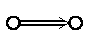
\includegraphics[width=0.34\textwidth]{figures/Fig_092_PDF180_Book168.pdf}
  \caption{该例中的二顶点箭图（原书 p.168）}
\end{figure}
\end{example}

\begin{example}[五次多项式的 thimble]\label{ex:quintic-thimbles}
令 $W\colon\mathbb C\to\mathbb C$，$Z\mapsto \frac45Z^5+Z$。其临界点为 $\frac{\pm1\pm i}{2}$，临界值为 $\frac{2(\pm1\pm i)}{5}$。基点 $1\in\mathbb C$ 上方的纤维由五个点组成。下图画出六条曲线 $\gamma_i$，它们从基点连向这些临界值。每条曲线对应一个 thimble $U_i$ 和一个消失圈 $V_i$；消失圈是两个点组成的集合，thimble 则是连接这两点的线段。

\begin{figure}[H]\centering
  \centering
  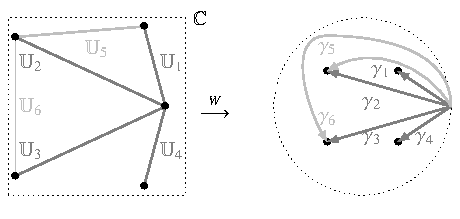
\includegraphics[width=0.84\textwidth]{figures/Fig_093_PDF180_Book168.pdf}
  \caption{五次多项式的临界值、thimble 与消失圈（原书 p.168）}
  \label{fig:quintic-thimbles}
\end{figure}

四元组 $\gamma_1,\ldots,\gamma_4$ 构成一个例外序列。在这个例子中，所有消失圈都包含同一个点，因此每对顶点之间都有态射。进一步考察可知，消失圈的自同态环是下列线性箭图的路径代数：
\begin{figure}[H]\centering
  \centering
  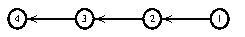
\includegraphics[width=0.43\textwidth]{figures/Fig_094_PDF180_Book168.pdf}
  \caption{例外序列对应的线性箭图（原书 p.168）}
  \label{fig:linear-quiver-exceptional-sequence}
\end{figure}
\[
  Q=\left(4\longleftarrow3\longleftarrow2\longleftarrow1\right).
\]

若将 $\gamma_2$ 绕 $\gamma_1$ 变异，便得到 $\gamma_5$；若先将 $\gamma_3$ 绕 $\gamma_2$ 变异，再绕 $\gamma_1$ 变异，也会得到 $\gamma_6$。
% [Tutor Note: 原书 p.169 此处两处均作“变成 $\gamma_5$”，但同段随即写“以 $\gamma_5,\gamma_6$ 替换 $\gamma_2,\gamma_3$”，且下一句按 $\gamma_6,\gamma_5$ 计顶点次序；第二次变异（先绕 $\gamma_2$、再绕 $\gamma_1$）应为 $\gamma_6$。译文径改，对照原书时请注意。]

以 $\gamma_5,\gamma_6$ 替换 $\gamma_2,\gamma_3$ 后，顶点次序发生交换，因为 $\gamma_6,\gamma_5$ 的起始角度小于 $\gamma_1$。此时只有相邻的消失圈相交，故自同态环成为对偶箭图代数（其中所有箭头乘积均为零）：
\begin{figure}[H]\centering
  \centering
  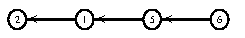
\includegraphics[width=0.43\textwidth]{figures/Fig_095_PDF181_Book169.pdf}
  \caption{变异后得到的线性箭图（原书 p.169）}
  \label{fig:mutated-linear-quiver}
\end{figure}
此时的箭图依次连接顶点 $2,1,5,6$，且相邻箭头的乘积均为零。
这两个代数都生成线性箭图的导出范畴。
\end{example}

\subsection{生成判据}\label{subsec:generation-criteria}
一般而言，判断一组拉格朗日膜是否分裂生成 Fukaya 范畴并不容易。锥的几何解释提示我们：要寻找分裂生成元，应当找到一组拉格朗日子流形，使每个拉格朗日子流形都能经 Hamilton 同伦变形到由这组子流形拼成的极限。

\begin{example}[曲面上的弧]
若 $X$ 是曲面，可以令这些拉格朗日子流形把曲面切分为拓扑平凡的区域，例如多边形或条带。比如，取一个带有标记点 $m_1,\ldots,m_k$ 的紧致黎曼曲面 $\Sigma$。删去标记点所得的曲面 $\Sigma^\times=\Sigma\setminus\{m_1,\ldots,m_k\}$，可通过在每个标记点附近挖去小圆盘并粘上无限圆柱，而获得 Liouville 流形结构。对连接两个标记点的每条曲线，我们在 $\mathrm{Fuk}^{\mathrm{wr}}\Sigma^\times$ 中得到一个非紧拉格朗日子流形，称为一条弧。下面给出了一个由四条弧分成两个正方形的双穿孔环面。

\begin{figure}[H]\centering
  \centering
  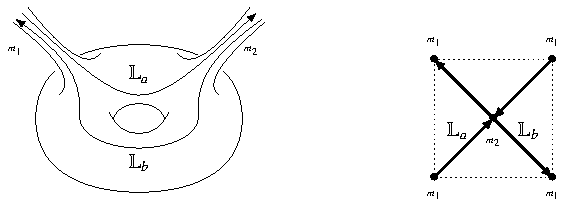
\includegraphics[width=0.77\textwidth]{figures/Fig_096_PDF181_Book169.pdf}
  \caption{弧将双穿孔环面分为两个正方形（原书 p.169）}
  \label{fig:arcs-two-punctured-torus}
\end{figure}

每条弧都可看作 wrapped Fukaya 范畴中的对象；弧之间的 Reeb 弦对应标记点周围的逆时针角。一个角的锥会把两条弧粘成一条新弧。也可以用多个角之和的锥粘接两条以上的弧，从而得到带局部系统的闭曲线。
\end{example}

\begin{theorem}{曲面上弧的生成判据}{arcs-generate-surface-fukaya}
若一组弧把曲面 $\Sigma$ 切分为多边形，则这组弧生成 wrapped Fukaya 范畴 $D^\pi\mathrm{Fuk}^{\mathrm{wr}}\Sigma^\times$。
\end{theorem}
\begin{proof}[证明思路]
若这些弧将曲面切分为多边形，就可以用沿着曲线所经过的多边形边界行进的弧序列来逼近任意曲线。因此，借助锥构造，可以得到任意曲线。

\begin{figure}[H]\centering
  \centering
  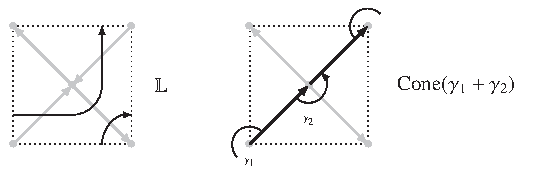
\includegraphics[width=0.72\textwidth]{figures/Fig_097_PDF182_Book170.pdf}
  \caption{通过角的锥拼接弧（原书 p.170）}
  \label{fig:cone-of-angles-arcs}
\end{figure}
\end{proof}

\begin{note}\label{note:surface-arcs-combinatorial}
\textbf{注 6.78.} 用弧生成曲面 Fukaya 范畴的思想将在本书第三部分进一步展开。它使我们能够组合地定义 Fukaya 范畴，并避开辛几何中大多数技术细节。
\end{note}

对于高维辛流形，情形更为复杂，因为拉格朗日膜并不会把流形切分为互不相交的区域。Abouzaid \bookcite{6} 给出了另一种检验一组拉格朗日膜是否生成 wrapped Fukaya 范畴的方法。其基本思想是：要成为分裂生成元，膜之间的态射必须充分反映 Reeb 流。为测量这一点，我们需要比较两个复形。

\begin{definition}{Hochschild 同调}{hochchild-homology-generators}
设 $\{L_i\}_{i\in I}$ 是一组拉格朗日膜，$L$ 是它们在 Fukaya 范畴中直和 $\bigoplus_iL_i$ 的自同态代数。Hochschild 同调\index{hochschildtongdiao@Hochschild 同调|hyperpage} $HH_\bullet(L)$ 定义为复形
\[
  CC_\bullet:=\bigoplus_{k=0}^{\infty}L\otimes L[1]^{\otimes k}
\]
的同调，其中微分由各个 $A_\infty$ 乘积给出：
\[
\begin{aligned}
 d(\gamma_0\otimes\cdots\otimes\gamma_k)
 ={}&\sum_{i>j}\pm\mu(\gamma_i,\ldots,\gamma_k,\ldots,\gamma_j)
       \otimes\gamma_{j+1}\otimes\cdots\otimes\gamma_{i-1}\\
 &+\sum_{i<j}\pm\gamma_0\otimes\cdots\otimes\gamma_i
       \otimes\mu(\gamma_{i+1},\ldots,\gamma_j)
       \otimes\gamma_{j+1}\otimes\cdots\otimes\gamma_k.
\end{aligned}
\]
% [Tutor Note: 这里已把第一个和式中的指标改为 $\gamma_{j+1}\otimes\cdots\otimes\gamma_{i-1}$：当 $\mu$ 作用于循环区间 $\gamma_i,\ldots,\gamma_k,\gamma_0,\ldots,\gamma_j$ 时，余下恰是 $\gamma_{j+1},\ldots,\gamma_{i-1}$；原文 p.170 印作 $\gamma_{i+j+1}$，疑为笔误。另外 Hochschild 同调在此记作 $HH_\bullet$，与 $CC_\bullet$ 的下标一致。]
\end{definition}

\begin{note}\label{note:hochchild-general}
\textbf{注 6.80.} Hochschild 同调是代数对象，对任意 $A_\infty$ 代数或范畴都可以定义\bookcite{253,93}。对多项式环 $\mathbb C[X_1,\ldots,X_n]$，它同构于多项式微分形式环
\[
  \mathbb C[X_1,\ldots,X_n]\langle dX_1,\ldots,dX_n\rangle.
\]
这称为 Hochschild--Kostant--Rosenberg 定理\bookcite{160,253}，并且对所有光滑仿射簇的坐标环都成立（见第\ref{ch:algebraic-geometry}章）。
\end{note}

\begin{definition}{辛同调}{symplectic-homology-generation}
设 $(X,\theta)$ 是带柱形端的 Liouville 流形。辛同调\index{xintongdiao@辛同调|hyperpage}是复形 $SC^\bullet(X)$ 的同调。该复形由某个适当通有的含时 Hamilton 函数所对应的 Reeb 流轨道生成，微分通过计数伪全纯圆柱定义：
\[
  d\rho_1=\sum_{\rho_2}\sum_{\psi\in\mathcal M(\rho_1,\rho_2)}\sigma_\psi\,\rho_2,
\]
其中 $\mathcal M(\rho_1,\rho_2)$ 表示连接 $\rho_1$ 与 $\rho_2$ 的刚性伪全纯圆柱模空间，$\sigma_\psi$ 是相应的符号。
\begin{figure}[H]\centering
  \centering
  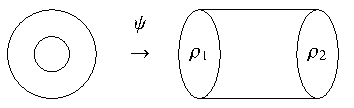
\includegraphics[width=0.48\textwidth]{figures/Fig_098_PDF183_Book171.pdf}
  \caption{辛同调微分所计数的伪全纯圆柱（原书 p.171）}
  \label{fig:symplectic-homology-cylinder}
\end{figure}
\end{definition}

\begin{note}\label{note:symplectic-homology-ainfty}
\textbf{注 6.82.} 辛同调带有 $A_\infty$ 结构，该结构通过计数从单位圆盘出发、挖去若干小圆盘的全纯映射得到；在此结构下，它还具有一个同伦意义下的单位元。关于辛同调的更多内容，见文献\bookcite{53,78,255,182}。
\end{note}

\begin{definition}{开闭映射}{open-closed-map}
开闭映射\index{kaibiyingshe@开闭映射|hyperpage} $OC\colon CC_\bullet(L)\to SC^\bullet(X)$ 通过计数以 Reeb 弦为角点、以 Reeb 轨道为另一端的带符号全纯映射 $\psi$ 定义：
\[
  OC(\gamma_1\otimes\cdots\otimes\gamma_k)=\sum_{\rho}\sum_{\psi\in\mathcal M(\gamma_1,\ldots,\gamma_k;\rho)}\sigma_\psi\,\rho.
\]
这里 $\mathcal M(\gamma_1,\ldots,\gamma_k;\rho)$ 是具有指定 Reeb 弦角点及 Reeb 轨道端的全纯映射模空间，$\sigma_\psi$ 表示其符号。
\begin{figure}[H]\centering
  \centering
  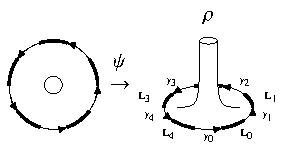
\includegraphics[width=0.62\textwidth]{figures/Fig_099_PDF183_Book171.pdf}
  \caption{开闭映射所计数的全纯曲面（原书 p.171）}
  \label{fig:open-closed-map}
\end{figure}
该映射是复形间的态射，因而在同调上诱导映射
\[
  OC\colon HH_\bullet(L)\longrightarrow SH^\bullet(X).
\]
% [Tutor Note: 开闭映射是链映射并不显然：需把“一端为 Reeb 轨道、另一端为若干 Reeb 弦”的圆柱模空间紧化，使其边界项分别对应 Hochschild 微分与辛同调微分；为此要对含时 Hamilton 函数取一般位置，否则会出现伪全纯圆柱的破裂。原文把验证留给文献 6。]
\end{definition}

\begin{theorem}{Abouzaid 生成判据}{abouzaid-generation-criterion}
若单位元 $1\in SH^\bullet(X)$ 属于 $OC$ 的像，则 $\{L_i\}_{i\in I}$ 分裂生成 $X$ 的 wrapped Fukaya 范畴。
\end{theorem}
\begin{proof}[证明思路]
给定任意拉格朗日膜 $B$，由该判据可找到一组高阶乘积，使得
\[
  1_B=\sum_r\mu(\gamma_{r,1},\ldots,\gamma_{r,k_r}).
\]
引理\ref{lem:split-generation-criterion} 随即说明 $B$ 由 $L$ 分裂生成。
\end{proof}

\begin{example}[圆柱上的 Abouzaid 判据]
Abouzaid 判据最基本的例子\bookcite{6} 是 $X=T^*S^1$。此时余切纤维 $T_x^*M$ 是生成元。$L=\mathbb C[X^{\pm1}]$ 的 Hochschild 同调为微分形式环 $\mathbb C[X^{\pm1}]\langle dX\rangle$，其中 $dX$ 简记为 $1\otimes X-X\otimes1$。

在辛同调中，绕圆柱 $i$ 圈的每个 Reeb 轨道 $\gamma_i$ 给出两个元素 $\gamma_i[0],\gamma_i[1]$，其次数分别为 $0$ 和 $1$。（若 Hamilton 函数与时间无关，闭 Reeb 轨道会产生一圈起点各异的 Reeb 轨道；对 Hamilton 函数作扰动后，这个圆周对称性破缺，只留下两个轨道。）当 $i=0$ 时，这两个元素对应于流为零处的“常值环路”。所以每个次数和同调类恰好各有一个基元素。开闭映射保持这两种分次，并给出同构，将 $X^i$ 映到 $\gamma_i[0]$，将 $X^idX$ 映到 $\gamma_i[1]$。
\end{example}

\begin{note}\label{note:compact-generation-criterion}
\textbf{注 6.86.} 预期紧致辛流形的 Fukaya 范畴也存在相应版本的生成判据；在这种情形下，辛同调由量子上同调取代。
\end{note}

\section{习题}\label{sec:fukaya-exercises}
\begin{exercise}\label{exer:morse-torus}
令 $T=\mathbb R^2/2\pi\mathbb Z^2$。选取适当的 Morse 函数，例如 $(\theta_1,\theta_2)\mapsto\cos(\theta_1)+2\sin(\theta_2)$，求 $T$ 的 Morse 上同调。
\end{exercise}

\begin{exercise}\label{exer:cotangent-geodesic-flow}
设流形 $M$ 带有度量 $g$，它在辛流形 $T^*M$ 上定义 Hamilton 函数 $h=g^{ij}p_ip_j$。
\begin{enumerate}[label=(\roman*)]
  \item 令 $M=\mathbb R^2/2\pi\mathbb Z^2$，取由 $\mathbb R^2$ 标准度量诱导的度量，并选 $x\in M$。证明 $T_x^*M$ 与 $\phi_h^t(T_x^*M)$ 横截相交，并描述交集。
  \item 令 $M$ 为由 $\mathbb R^3$ 中标准嵌入诱导度量的单位球面，并选 $x\in M$。证明 $T_x^*M$ 与 $\phi_h^t(T_x^*M)$ 并非横截相交。
\end{enumerate}
\end{exercise}

\begin{exercise}\label{exer:liouville-pants}
求一个 $\theta$，使 $\mathbb C\setminus\{0,1\}$ 成为在 $0,1,\infty$ 处有三个柱形端的 Liouville 流形。利用这一构造，通过把穿孔曲面切分成裤子曲面，为任意亏格和任意穿孔数的穿孔曲面构造 Liouville 流形结构。
\end{exercise}

\begin{exercise}\label{exer:surface-fukaya-endomorphisms}
设亏格为 $g$、有 $n$ 个穿孔的曲面带有在穿孔处具有柱形端的 Liouville 结构，并假设 $(g,n)\ne(0,1),(0,2)$。
\begin{enumerate}[label=(\roman*)]
  \item 证明：若 $\gamma$ 是一条非可缩简单闭曲线，则存在一条与 $\gamma$ 同位且正合的曲线 $\gamma'$。证明，对应于这个拉格朗日子流形（取平凡自旋结构）的对象在正合 Fukaya 范畴中的自同态环为 $\mathbb C[\varepsilon]/(\varepsilon^2)$，且 $\deg_{\mathbb Z_2}\varepsilon=1$。
  \item 设 $\gamma$ 是一条两端分别趋于不同穿孔的开拉格朗日子流形。证明，对应对象在 wrapped Fukaya 范畴中的自同态环为 $\mathbb C[X,Y]/(XY)$，且 $\deg_{\mathbb Z_2}X=\deg_{\mathbb Z_2}Y=1$。
\end{enumerate}
\end{exercise}

\begin{exercise}\label{exer:stopped-pants}
把裤子曲面看成带柱形端的 Liouville 流形，并在每个柱形端各放置一个 stop。
\begin{enumerate}[label=(\roman*)]
  \item 证明相应的 partially wrapped Fukaya 范畴是 Hom 有限的（即对象之间的 Hom 空间有限维）。
  \item 取三条彼此不相交的拉格朗日子流形，它们都具有柱形端，并分别连接不同的一对柱形端。描述这三者的自同态环。依 stop 的位置不同，有多少种可能？
  \item 描述移去 stop 后这个自同态环会发生什么变化。
\end{enumerate}
\end{exercise}

\begin{exercise}\label{exer:stopped-cotangent-torus}
令 $X=T^*T$，其中 $T$ 是实环面。取环面上的位置坐标 $q_1,q_2$ 和余切方向的动量坐标 $p_1,p_2$，并将 $X$ 视为带柱形端的 Liouville 流形。
\begin{enumerate}[label=(\roman*)]
  \item 令 $x\in T\subset T^*T$。描述从 $L=T_x^*T$ 到自身的 Reeb 弦，并解释其自同态环为集中在 $\mathbb Z_2$ 次数 $0$ 的 $\mathbb C[\mathbb Z^2]$。
  \item 对每个点 $y\in T$ 及每个本原向量 $v\in\mathbb Z^2$，可在 $T$ 中画一条过 $y$、法向量为 $v$ 的直线。构造一个 stop，使得投影沿 $v$ 方向穿过这条直线的每个 Reeb 弦都具有正次数。
  \item 若 $v_1,\ldots,v_k\in\mathbb Z^2$ 是本原向量，且 $y_1,\ldots,y_k,x\in T$ 互不相同，证明：在对每一对 $(y_i,v_i)$ 都设 stop 的 partially wrapped Fukaya 范畴中，$L_x=T_x^*T$ 的自同态环为
  $\mathbb C[u\in\mathbb Z^2\mid\langle v_i,u\rangle\le0]$。
\end{enumerate}
\end{exercise}

\begin{exercise}\label{exer:xy-z3-plus-z}
考察函数 $f\colon\mathbb C^3\to\mathbb C$，$(X,Y,Z)\mapsto XY-Z^3+Z$。
\begin{enumerate}[label=(\roman*)]
  \item 求 $f$ 的临界点和临界值。
  \item 构造连接基点 $1\in\mathbb C$ 与临界值的直线所对应的消失圈和 thimble。消失圈之间如何相交？
  \item 解释有向 Fukaya 范畴为何等价于 $D\mathrm{mod}^{\pm}Q$，其中 $Q$ 为下图所示的箭图。
\end{enumerate}
\begin{figure}[H]\centering
  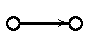
\includegraphics[width=0.34\textwidth]{figures/Fig_100_PDF185_Book173.pdf}
  \caption{练习 6.7 中的箭图 $Q$（原书 p.173）}
\end{figure}
\end{exercise}

\begin{exercise}\label{exer:quintic-all-orientations}
令 $W\colon\mathbb C\to\mathbb C$，$Z\mapsto\frac45Z^5+Z$，如例\ref{ex:quintic-thimbles}所述。对线性箭图 $L_4$ 的每一种箭头定向，求一组生成元，使其自同态环为该箭图的路径代数。
\end{exercise}

\begin{exercise}\label{exer:z2-zminus1-generators}
令 $W\colon\mathbb C^*\to\mathbb C$，$Z\mapsto Z^2+Z^{-1}$。求有向 Fukaya 范畴的一组生成元，并描述其自同态环。
\end{exercise}

\begin{exercise}\label{exer:two-sided-stops}
考察 $T^*S^1$，在一端放置 $k$ 个 stop，在另一端也放置 $k$ 个 stop。令 $L_{i,0}$ 是一条拉格朗日子流形，其一端从第一端第 $i$ 个与第 $i+1$ 个 stop 之间出发，另一端也止于第二端第 $i$ 个与第 $i+1$ 个 stop 之间；令 $L_{i,1}$ 从相同区间出发，但在另一端止于再往前一个区间（即第 $i+1$ 与第 $i+2$ 个 stop 之间）。
\begin{enumerate}[label=(\roman*)]
  \item 通过用这些曲线取锥来逼近任意曲线，证明它们生成 partially wrapped Fukaya 范畴。
  \item 计算这些拉格朗日子流形的自同态环。
  \item 现在考察 $W\colon\mathbb C^*\to\mathbb C$，$Z\mapsto Z^k+Z^{-k}$。解释这个 Lefschetz 纤维化的有向 Fukaya 范畴为何等价于本题中的 partially wrapped Fukaya 范畴。
\end{enumerate}
\end{exercise}

\chapterreview{%
\textbf{全章地位。}本章是同调镜像对称 A 侧的定义章。它先用开篇的 Morse 理论当练习场，让读者在有限维、可计算的设定里看清“复形—微分—分次”三件事，再把同一套机器搬到辛流形上，构造出基本 Fukaya 范畴，并依次给出 wrapped、partially wrapped、有向、相对、完整五种变体，最后讨论生成元。后文的曲面组合模型与所有 A 侧计算都以本章为入口。

\textbf{知识脉络。}Morse 复形由临界点张成，微分统计指数相差 $1$ 的流轨迹，$d^2=0$ 来自单参数轨迹族两端的符号相消；把 $M$ 换成余切丛的零截面、把梯度流换成 Hamilton 流，同一复形改由 $M$ 与 $\phi_\epsilon^hM$ 的交点张成，微分统计全纯二边形，Morse 指数随之变成交点的分次。若 Hamilton 函数只含动能项，交点便编码闭测地线，复形转而计算环路空间同调。把这一图景放到带柱状端的 Liouville 流形上：对象取正合紧致拉格朗日子流形，态射由横截交点张成，高阶积计数满足边界条件的伪全纯多边形；正合性保证面积由边界势差控制、求和有限，并排除泡，于是得到 $\mathbb Z_2$ 分次的 $A_\infty$ 预范畴，存在复体积形式时可提升为 $\mathbb Z$ 分次。变体一节再逐层放宽：允许浸入与局部系统；纳入非紧对象（wrapped，用 Reeb 弦与 $S_k$ 处理配对问题）；用 stop 截断 Reeb 流（partially wrapped，$U$-次数为零的态射，局部化）；用 Lefschetz 纤维化的 thimble 定义有向范畴；用除子与 Novikov 域处理紧致流形。

\textbf{核心结论。}（1）Morse 复形是上链复形，其上同调等于 $H^\bullet(M)$；在 $T^*M$ 中 $CF^\bullet(\phi_\epsilon^hM,M)$ 复现同一复形。（2）正合性使 Floer 乘积成为有限和：$\int_D\psi^*\omega=\sum_i\bigl(f_i(p_{i+1})-f_i(p_i)\bigr)$ 被紧致性控制；正合情形下两类泡都给出面积为零的映射，与 Gromov 紧致性矛盾，故 $\mu_k$ 满足 $A_\infty$ 关系。（3）$\mu_k$ 的次数为 $2-k$，交点次数为 $\deg x=(\Delta-(\theta_2-\theta_1))/\pi$；一般只有 $\mathbb Z_2$ 分次，Calabi--Yau 流形上可取 $\mathbb Z$ 分次。（4）包含链 $\mathrm{exFuk}^\bullet\subset\mathrm{wrFuk}^\bullet$；$\mathrm{wrFuk}^\bullet(T^*M)$ 由单个余切纤维生成，且 $D^\pi\mathrm{Fuk}^{\mathrm{wr}}T^*M\simeq D^\pi H^\bullet(\mathcal L_xM)$。（5）生成判据：若单位元 $1\in SH^\bullet(X)$ 落在开闭映射 $OC$ 的像中，则这组拉格朗日膜分裂生成 wrapped Fukaya 范畴。

\textbf{辨析与提醒。}其一，正合不是辛流形的一个技术条件，而是要求 $\theta$ 整体存在，因此正合辛流形必非紧致（否则 $\omega^n$ 是体积形式却上同调为零）；相对范畴与完整范畴正是为紧致流形补这个洞。其二，$\mathbb Z_2$ 与 $\mathbb Z$ 分次的差别不是记账问题：交点次数依赖 $\Omega$ 的相位沿路径的单值性，$\Omega=z^kdz$ 在 $k\ne-1$ 时甚至不给出底圆的分次，基本范畴为空。其三，wrapped 与普通 Fukaya 范畴的关系类似“有限生成模与有限维模”，partially wrapped 则是把某个子范畴的态射取逆的局部化；对象集逐层扩大，不能用同一套直觉混用。其四，定向与自旋结构、符号 $\sigma_\psi$ 是 $A_\infty$ 关系成立的实质条件，只有在 $\operatorname{char}k=2$ 时才可以暂时忽略。

\textbf{评注。}作者选择“Morse $\to$ Fukaya”的路线是有代价的：正文从未真正写下虚拟基本类或含时扰动的完整定义，模空间的光滑性、$S_k$ 的相干性、$k[[G]]$ 不是域时的极小模型，都只用“应当可以”“技术上相当复杂”带过。但这一取舍换来了全书最清晰的一条主线——读者始终知道每个定义是为解决哪个具体障碍而设：泡逼出正合性与带曲率结构，非紧对象逼出 wrapped，紧致流形逼出相对与完整范畴。真正该记住的不是定义本身，而是两个构造：拉格朗日手术即锥（$L_1+_xL_2\cong\operatorname{Cone}(x)$）与开闭映射检测生成。局限也要看清：曲面上用弧切分多边形得到的组合模型极其漂亮，却不能外推到高维，高维情形必须回到 Abouzaid 判据；而完整 Fukaya 范畴在本章只是框架，要做具体计算，仍应回到正合或相对设定。}

\chapter{B 侧}\label{ch:algebraic-geometry}
本章介绍 $B$ 模型所涉及的范畴：相干层的导出范畴与奇点范畴。这里的讲法与通常的导出范畴入门略有不同，因为我们希望把它定义为一个 $A_\infty$ 范畴。为此需要给范畴选择一个增强；我们将通过局部自由层的层上同调来构造这种增强。代数几何的背景知识可参阅\bookcite{109,74,248}；关于（拟）相干层导出范畴的经典处理，可参阅\bookcite{186,185,157}。

\section{簇}\label{sec:varieties}
\takeaway{簇是仿射环反等价意义下的空间，经 Zariski 开集粘合而成；拟相干层即 $R$-模的层化，局部自由层对应向量丛。Čech 复形计算层上同调，局部自由分解的 Hom 复形给出 $A_\infty$ 增强 $\mathrm{Coh}^{\bullet}X$；光滑性等价于 $\mathrm{Perf}^{\bullet}X\subset D\mathrm{Coh}^{\bullet}X$ 是等价。}
\subsection{仿射环与仿射簇}\label{subsec:affine-rings-varieties}
代数几何的基本思想，是把代数看作某个空间上的函数环。由此，环与空间之间便出现一种对偶关系；对一类特殊的环，这种对偶关系可以精确表述。

\begin{definition}{仿射环}{affine-ring}
仿射环\index{fangshehuan@仿射环|hyperpage}是一个有限生成、无幂零元的交换 $\mathbb C$-代数。由这些环及其 $\mathbb C$-代数态射组成的范畴记为 $\mathrm{AffRing}$。
\end{definition}

设 $R$ 是仿射环，例如
\[
  R=\frac{\mathbb C[X_1,\ldots,X_n]}{(f_1,\ldots,f_k)}.
\]
集合
\[
  V(R):=\mathrm{AffRing}(R,\mathbb C)
\]
由所有一维表示 $\rho\colon R\to\mathbb C$ 组成。把 $\rho$ 对应到点 $(\rho(X_1),\ldots,\rho(X_n))\in\mathbb C^n$，便可将 $V(R)$ 识别为 $\mathbb C^n$ 的子集：
\[
  V(R)\cong\{x\in\mathbb C^n\mid f_1(x)=\cdots=f_k(x)=0\}.
\]

环态射 $\phi\colon R\to S$ 诱导连续映射
\[
  V(\phi)\colon V(S)\longrightarrow V(R),\qquad \rho\longmapsto\rho\circ\phi.
\]

\begin{definition}{仿射簇及仿射映射}{affine-varieties}
范畴 $\mathrm{AffVar}$ 的对象是所有 $V(R)$，态射是所有 $V(\phi)$。这些对象称为仿射簇\index{fangshecu@仿射簇|hyperpage}，态射称为仿射映射\index{fangsheyingshe@仿射映射|hyperpage}。
\end{definition}

\begin{example}[仿射空间与抛物线]
若 $R=\mathbb C[X_1,\ldots,X_n]$，则称 $V(R)$ 为 $n$ 维仿射空间\index{fangshekongjian@仿射空间|hyperpage}，记为 $\mathbb A^n$；作为集合，它就是 $\mathbb C^n$。态射
\[
  \phi\colon\mathbb C[X,Y]\to\mathbb C[X],\qquad
  f(X,Y)\longmapsto f(X,X^2)
\]
诱导仿射映射
\[
  V(\phi)\colon\mathbb A^1\longrightarrow\mathbb A^2,
  \qquad x\longmapsto(x,x^2),
\]
它把仿射直线映到 $\mathbb A^2$ 中的一条抛物线上。
\end{example}

环 $R$ 本身也可以看作 $V(R)$ 上的函数环：每个 $r\in R$ 都定义一个函数
\[
  \mathrm{ev}_r\colon V(R)\to\mathbb C,\qquad \rho\longmapsto\rho(r).
\]
这提示我们应当能够从 $V(R)$ 重建 $R$。事实上，对 $\mathrm{AffVar}$ 中任意对象 $X$，定义
\[
  \mathcal O(X):=\mathrm{AffVar}(X,\mathbb A^1),
\]
其中 $\mathbb A^1=V(\mathbb C[X])$ 视为 $\mathbb C$。由于 $\mathbb A^1$ 上有加法与乘法，集合 $\mathcal O(X)$ 也具有环结构。若 $\phi\colon X\to Y$ 是仿射映射，则可定义环态射
\[
  \mathcal O(\phi)\colon\mathcal O(Y)\to\mathcal O(X),
  \qquad f\longmapsto f\circ\phi.
\]
由此，$\mathcal O$ 成为反变函子。

\begin{theorem}{仿射环与仿射簇的反等价}{affine-rings-varieties-antiequivalence}
函子 $V$ 与 $\mathcal O$ 给出反等价：
\[
\begin{array}{c}
  \mathrm{AffRing}\ \underset{\mathcal O}{\overset{V}{\rightleftarrows}}\ \mathrm{AffVar}.
\end{array}
\]
\end{theorem}
\begin{proof}[证明思路]
这是 Hilbert 零点定理的一种范畴化表述。该定理说明映射
\[
  R\longrightarrow\mathcal O(V(R)),\qquad r\longmapsto\mathrm{ev}_r
\]
是同构。这里 $R$ 无幂零元这一假设至关重要，因为对幂零元 $r$，函数 $\mathrm{ev}_r$ 会恒为零。
\end{proof}

\begin{figure}[H]\centering
  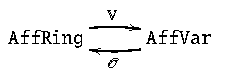
\includegraphics[width=0.48\textwidth]{figures/Fig_101_PDF188_Book176.pdf}
  \caption{仿射环与仿射簇之间的反等价（原书 p.176）}
  \label{fig:affring-affvar-antiequivalence}
\end{figure}

\subsection{模作为层}\label{subsec:modules-as-sheaves}
设 $R$ 是仿射环，$g\in R$。态射 $\iota\colon R\to R[g^{-1}]$ 诱导映射 $V(\iota)\colon V(R[g^{-1}])\to V(R)$。该映射是一个嵌入，其像为
\[
  U_g=\{\rho\in V(R)\mid \rho(g)\ne0\}.
\]
这类子集称为仿射开集\index{fangshekaiji@仿射开集|hyperpage}，它们生成 $X=V(R)$ 上的一种拓扑，称为 Zariski 拓扑\index{zariskituopu@Zariski 拓扑|hyperpage}。注意，两个仿射开集的交仍是仿射开集，且 $U_g\cap U_h=U_{gh}$；但仿射开集的并却未必是仿射的。

\begin{definition}{开集范畴}{open-category}
范畴 $\mathrm{Open}(X)$ 的对象是 $X$ 的所有 Zariski 开集\index{zariskikaiji@Zariski 开集|hyperpage}，态射是包含映射。仿射开集组成的全子范畴记为 $\mathrm{AffOpen}(X)$。
\end{definition}

\begin{note}\label{note:zariski-topology}
\textbf{注 7.6.} $V(R)$ 作为 $\mathbb C^n$ 子集所继承的通常拓扑，比 Zariski 拓扑精细得多。一般而言，Zariski 拓扑不是 Hausdorff 的。事实上，若 $R$ 没有零因子，则每个非空 Zariski 开集都是稠密的。
\end{note}

设 $M$ 是一个 $R$-模，$\rho\colon R\to\mathbb C$ 是 $X=V(R)$ 中一点，则张量积
\[
  M_\rho:=M\otimes_\rho\mathbb C
  =\frac{M\otimes\mathbb C}{(mr\otimes1-m\otimes\rho(r)\mid r\in R)}
\]
是一个 $\mathbb C$-向量空间。让 $\rho$ 变化，便得到一个定义在 $X$ 上的“向量丛\index{xiangliangcong@向量丛|hyperpage}”；不过，与向量丛不同，$M_\rho$ 的维数可能随 $\rho\in X$ 改变。

$M$ 中的每个元素 $m$ 都给出向量 $m\otimes1\in M_\rho$，因而可视为这个“丛”的一个截面。把它限制到仿射开集 $U_g\subset X$ 上时，$M\otimes_RR[g^{-1}]$ 中的元素可解释为局部截面，因为
\[
  m\otimes g^{-1}(\rho)=m\otimes\rho(g)^{-1}\in M_\rho.
\]
若两个仿射开集包含关系为 $U_g\subset U_h$，则 $R[h^{-1}]\subset R[g^{-1}]$，并有一个反向的限制映射
\[
  M(U_h)\longrightarrow M(U_g),\qquad
  M\otimes_RR[h^{-1}]\longrightarrow M\otimes_RR[g^{-1}].
\]
因此，$M$ 给出一个反变函子 $\mathrm{AffOpen}(X)\to\mathrm{Vect}_{\mathbb C}$（也可以取值于 $\mathrm{Mod}_R$）。回忆例\ref{ex:geometric-modules}：从 $\mathrm{Open}(X)$ 出发的反变函子称为预层\index{ceng@层|hyperpage}。若要把 $M$ 扩展为定义在整个 $\mathrm{Open}(X)$ 上的函子，就需要确定非仿射开集上的取值。其思路是把截面粘合起来。

具体地，设 $\mathcal S\colon\mathrm{Open}(X)\to\mathrm{Vect}_{\mathbb C}$ 是一个预层，令 $U=\bigcup_{i\in I}U_i$ 是开覆盖，并记 $U_{ij}=U_i\cap U_j$。由这些数据可构造两个映射
\[
  \mathcal S(U)\xrightarrow{\iota}\prod_i\mathcal S(U_i)
  \xrightarrow{\delta}\prod_{i<j}\mathcal S(U_{ij}),
\]
其中
\[
  \iota(x)=\bigl(\mathcal S(U_i\hookrightarrow U)(x)\bigr)_{i\in I},
\]
而
\[
  \delta((x_i)_{i\in I})_{ij}
  =\mathcal S(U_{ij}\hookrightarrow U_i)(x_i)
   -\mathcal S(U_{ij}\hookrightarrow U_j)(x_j).
\]
第二个映射检验局部截面 $(x_i)_{i\in I}$ 是否在交叠处彼此相容。若这些 $x_i$ 都来自 $U$ 上的一个截面，当然相容，故 $\delta\iota=0$。但可能存在属于 $\ker\delta$ 却不属于 $\operatorname{im}\iota$ 的元素；这说明 $\mathcal S(U)$ 中缺少某些截面。

\begin{definition}{层}{sheaf}
若对每个开覆盖 $U=\bigcup_{i\in I}U_i$，都有 $\ker\delta=\operatorname{im}\iota$，则称预层 $\mathcal S\colon\mathrm{Open}(X)\to\mathrm{Vect}_{\mathbb C}$ 为一个层。
\end{definition}

\begin{lemma}{模预层的层化}{module-presheaf-sheaf}
函子 $M\colon\mathrm{AffOpen}(X)\to\mathrm{Vect}_{\mathbb C}$ 可以扩展为层 $M\colon\mathrm{Open}(X)\to\mathrm{Vect}_{\mathbb C}$。
\end{lemma}
\begin{proof}[证明思路]
对任意开集 $U$，取所有包含于 $U$ 的仿射开集作为覆盖，并定义 $M(U)$ 为相应映射 $\delta$ 的核。
\end{proof}

\begin{example}[仿射平面上的非仿射开集]
考察仿射平面 $\mathbb A^2=V(R)$，其中 $R=\mathbb C[X,Y]$。开集
\[
  U=U_X\cup U_Y=\mathbb A^2\setminus\{(0,0)\}
\]
不是仿射开集。取 $M=R$，则 $M(U)$ 中的局部截面对应于一对函数
\[
  (f(X,Y),g(X,Y))\in M(U_X)\times M(U_Y)
  =R[X^{-1}]\times R[Y^{-1}],
\]
它们在 $M(U_{XY})=R[X^{-1},Y^{-1}]$ 中相等。这意味着 $f$ 不含 $X$ 的负次幂，$g$ 不含 $Y$ 的负次幂；因而二者都属于 $R$。所以 $M(U)\cong R$。
\end{example}

\begin{definition}{拟相干层与相干层}{quasicoherent-coherent-sheaf}
若层 $M\colon\mathrm{Open}(X)\to\mathrm{Vect}_{\mathbb C}$ 来自某个 $R$-模 $M$，则称其为拟相干层\index{xiangganceng@相干层|hyperpage}\index{nixiangganceng@拟相干层|hyperpage}；若 $M$ 有限生成，则称其为相干层。
\end{definition}

\begin{example}[点上的点层]
设一维模 $M=\mathbb C$ 上的 $R$-作用由表示 $\sigma\colon R\to\mathbb C$ 给出。向量空间 $M_\rho$ 在 $\rho=\sigma$ 时为一维，在其他情形下为零维。同样，$M$ 在 $U_g$ 上的截面空间，当且仅当 $\sigma\in U_g$ 时为一维，否则为零维。对非仿射开集也如此。这个相干层 $M$ 称为支撑在 $\sigma$ 上的点层。
\end{example}

\begin{example}[秩一自由层]
若 $M=R$，那么对 $V(R)$ 中每个点 $\rho$，向量空间 $M_\rho$ 都是一维；而 $U_g$ 上的截面空间为 $\mathcal O(U_g)=R[g^{-1}]$。相干层 $M$ 称为秩一自由层\index{zhiyiziyouceng@秩一自由层|hyperpage}，它表示 $V(R)$ 上的平凡秩一向量丛。
\end{example}

\begin{definition}{结构层}{structure-sheaf}
秩一自由层还可以看作一个环层\index{huanceng@环层|hyperpage}，因为每个 $\mathcal O(U)$ 都有环结构。把它称为 $X$ 的结构层\index{jiegouceng@结构层|hyperpage}，记作 $\mathcal O_X$。若 $M$ 是任意 $R$-模，则层 $M$ 是一个 $\mathcal O_X$-模层\index{oxmoceng@O\_X-模层|hyperpage}：对每个开集 $U$，$M(U)$ 都是 $\mathcal O_X(U)$-模。
\end{definition}

\subsection{粘合簇}\label{subsec:gluing-varieties}
正如可以把 $\mathbb R^n$ 的不同开片粘合成流形，我们也可以尝试把不同仿射簇粘合成更大的簇。先取一个空间 $X=U_1\cup\cdots\cup U_r$，使每个 $U_i$ 都是仿射簇，其坐标环为 $R_i=\mathcal O(U_i)$，并且任意交集 $U_{ij}=U_i\cap U_j$ 都是 $U_i$ 与 $U_j$ 中的仿射开集。交集的坐标环
\[
  R_{ij}:=\mathcal O(U_{ij})
\]
可写成 $R_i[g_{ij}^{-1}]$ 与 $R_j[g_{ji}^{-1}]$，其中 $g_{ij}\in R_i$、$g_{ji}\in R_j$ 是某些函数。于是得到限制态射
\[
  R_i\longrightarrow R_i[g_{ij}^{-1}]
  =R_{ij}=R_j[g_{ji}^{-1}]\longleftarrow R_j.
\]

固定这些数据之后，对高阶交集 $U_{i_1\cdots i_k}$ 也可定义坐标环
\[
  R_{i_1\cdots i_k}
  =R_{i_1}[g_{i_1i_2}^{-1},\ldots,g_{i_1i_k}^{-1}],
\]
并对所有包含关系 $U_{j_1\cdots j_\ell}\subset U_{i_1\cdots i_k}$ 定义限制态射
\[
  R_{i_1\cdots i_k}\longrightarrow R_{j_1\cdots j_\ell}.
\]

所有 $U_i$ 中的仿射开集生成 $X$ 上的 Zariski 拓扑；同样可以定义范畴 $\mathrm{Open}(X)$。空间 $X$ 带有一个自然的环层 $\mathcal O_X$，称为结构层，并满足
\[
  \mathcal O_X(U_{i_1\cdots i_k})=R_{i_1\cdots i_k}.
\]
每个开集 $U_i$ 都有一个全忠实嵌入 $\iota_i\colon\mathrm{Open}(U_i)\hookrightarrow\mathrm{Open}(X)$，而 $\mathcal O_X\circ\iota_i$ 就是 $U_i$ 上的结构层 $\mathcal O_{U_i}$。

\begin{definition}{带仿射覆盖的簇}{variety-affine-cover}\index{daifangshefugaidecu@带仿射覆盖的簇|hyperpage}
二元组 $(X,\mathcal O_X)$ 称为一个簇，其仿射覆盖为 $\mathcal U=\{U_1,\ldots,U_r\}$。\footnote{与流形的情形类似，为使一切良好，还需要对覆盖施加一些额外条件（例如分离性），这里不再讨论。}
\end{definition}

\begin{example}[射影空间]
射影空间 $\mathbb P^n$ 由 $\mathbb C^{n+1}$ 的所有一维子空间组成。我们用 $(x_0:\cdots:x_n)\in\mathbb P^n$ 表示子空间 $\mathbb C(x_0,\ldots,x_n)\subset\mathbb C^{n+1}$。它可由 $n+1$ 个开集覆盖：
\[
  U_i=\{(x_0:\cdots:x_n)\mid x_i\ne0\}
  =\left\{\left(\frac{x_0}{x_i}:\cdots:1:\cdots:\frac{x_n}{x_i}\right)\right\}
  \cong\mathbb C^n.
\]
坐标环 $\mathcal O(U_i)$ 可识别为多项式环 $\mathbb C[\xi_{ki}\mid k\ne i]$，其中 $\xi_{ki}$ 表示有理函数 $X_k/X_i$。在交叠处有嵌入
\[
  \mathbb C[\xi_{ki}\mid k\ne i]
  \longrightarrow \mathbb C[\xi_{ki}\mid k\ne i][\xi_{ji}^{-1}]
  =\mathbb C[\xi_{k\ell}\mid \ell=i,j]
  =\mathbb C[\xi_{kj}\mid k\ne j][\xi_{ij}^{-1}]
  \longleftarrow\mathbb C[\xi_{kj}\mid k\ne j].
\]
这足以计算 $\mathbb P^n$ 上的结构层：一般地，对 $\mathrm{Open}(\mathbb P^n)$ 中任意开集 $U$，有
\[
  \mathcal O(U)=\left\{\frac fg\in\mathbb C(X_0,\ldots,X_n)
  \ \middle|\ \deg f=\deg g,\ g(x)\ne0\text{ 对每个 }x\in U\right\}.
\]
第一个条件保证 $f/g$ 的值不依赖于代表元 $(x_0:\cdots:x_n)$；第二个条件保证 $f/g$ 在 $U$ 上有定义。
\end{example}

\begin{example}[射影簇与拟射影簇]
更一般地，设
\[
  R=\mathbb C[X_0,\ldots,X_n]/(f_1,\ldots,f_k)
\]
是正分次仿射整环（即 $\deg X_i\ge0$，且 $f_i$ 都是齐次元）。定义
\[
  U_i=V\bigl((R[X_i^{-1}])_0\bigr),
\]
并用包含关系
\[
  (R[X_i^{-1}])_0\longrightarrow
  (R[X_i^{-1},X_j^{-1}])_0\longleftarrow(R[X_j^{-1}])_0
\]
把这些开集粘合。由此得到的空间记作 $\mathbb P(R)$。
\end{example}

若 $R=\mathbb C[X_0,\ldots,X_n]$ 且所有 $X_i$ 的次数都是 $1$，则 $\mathbb P(R)=\mathbb P^n$。对次数均为 $1$ 的更一般的环 $R=\mathbb C[X_0,\ldots,X_n]/(f_1,\ldots,f_k)$，可将 $\mathbb P(R)$ 识别为
\[
  X=\{(x_0:\cdots:x_n)\in\mathbb P^n\mid f_i(x_0,\ldots,x_n)=0\}.
\]
这类簇称为射影簇\index{sheyingcu@射影簇|hyperpage}。若 $R$ 是多项式环，其中 $X_0,\ldots,X_k$ 的次数为 $1$，其余变量的次数为 $0$，则 $\mathbb P(R)=\mathbb P^k\times\mathbb A^{n-k}$。加入关系会截出子簇，称为拟射影簇\index{nisheyingcu@拟射影簇|hyperpage}。注意，并非所有簇都属于这一类。

直观地说，$(X,\mathcal O_X)$ 上的拟相干层应当是这样一种层：在局部看起来像仿射开集上的拟相干层。

\begin{definition}{簇上的（拟）相干层}{coherent-sheaf-on-variety}
若 $\mathcal O_X$-模层 $M$ 满足：对每个仿射开集 $U\subset X$，限制 $M|_{\mathrm{Open}(U)}$ 都是 $\mathcal O_U$ 上的拟相干层，则称 $M$ 为（拟）相干层。
\end{definition}

只需在一个仿射覆盖上检验上述条件。因此，要在 $X=\bigcup_iU_i$ 上构造拟相干层，需要给出以下数据：
\begin{itemize}
  \item 对每个 $U_i$，给出一个 $R_i$-模 $M_i$；
  \item 对每个 $U_{ij}$，给出一个 $R_{ij}$-模 $M_{ij}$ 和 $R_{ij}$-模同构
  \[
    M_i\otimes_{R_i}R_{ij}\xrightarrow{\pi_{ij}}M_{ij}
    \xleftarrow{\pi_{ji}}M_j\otimes_{R_j}R_{ij}.
  \]
\end{itemize}
这些数据给出 $U_i$ 上的拟相干层 $M_i$、$U_{ij}$ 上的拟相干层 $M_{ij}$ 和自然变换 $\pi_{ij}\colon M_i|_{\mathrm{Open}(U_{ij})}\to M_{ij}$。这些变换必须满足相容关系，才能在更高阶交集上作良好定义。\footnote{把这个相容条件明确写出来，是一道很好的练习。}固定所有这些数据后，对 $X$ 上的层 $M$ 定义
\[
  M(V)=\ker\delta,
\]
其中对每个开集 $V\subset X$，有映射
\[
  \begin{aligned}
  \delta\colon\prod_iM_i(V_i)&\longrightarrow\prod_{i<j}M_{ij}(V_{ij}),\\
  (x_i)_i&\longmapsto
  \bigl(\pi_{ij}M_i(V_{ij}\hookrightarrow V_i)(x_i)
       -\pi_{ji}M_j(V_{ij}\hookrightarrow V_j)(x_j)\bigr)_{ij},
  \end{aligned}
\]
这里 $V_i=V\cap U_i$，$V_{ij}=V\cap U_i\cap U_j$。换言之，$V$ 上的截面是各个 $V_i$ 上截面的粘合。由于 $\mathcal O_X(V)$ 的截面也以类似方式构造，可以证明 $M(V)$ 是 $\mathcal O_X(V)$-模，故 $M$ 是 $X$ 上的拟相干层。

\begin{example}[射影簇上的层与分次模]
设
\[
  R=\mathbb C[X_0,\ldots,X_n]/(f_1,\ldots,f_k)
\]
是正分次整环，$M$ 是一个 $\mathbb Z$-分次 $R$-模。在 $X=\mathbb P(R)$ 上定义层
\[
  M(U_{X_i})=(M\otimes_RR[X_i^{-1}])_0,
\]
并使用标准映射
\[
  (M\otimes_RR[X_i^{-1}])_0\longrightarrow
  (M\otimes_RR[X_i^{-1},X_j^{-1}])_0
  \longleftarrow(M\otimes_RR[X_j^{-1}])_0
\]
来粘合。取 $M=R$ 时得到 $\mathbb P(R)$ 上的结构层。若取 $M=R(k)$，其中 $R(k)_i=R_{i+k}$，则当 $k\ne0$ 时，新层 $\mathcal O(k)$ 不等于结构层 $\mathcal O$，因为它们的截面不同：
\[
  \mathcal O(k)(U_i)=R[X_i^{-1}]_k,
  \qquad \mathcal O(k)(\mathbb P^n)=R_k.
\]

不同的分次模可能给出相同的层。若 $M$ 是有限维 $R$-模，则当 $n$ 充分大时 $X_i^nM=0$，从而 $M\otimes_RR[X_i^{-1}]=0$。因此每个 $M(U_i)$ 都为零，故 $M$ 给出零层。类似地，若 $M$ 含有有限维分次子模 $N$，那么 $M$ 与 $M/N$ 所给出的层相同。

反过来，若 $M$ 是 $\mathbb P(R)$ 上的层，可以构造一个相应的分次模。先定义层 $M(k)$，使得对每个仿射开集 $U_i$，
\[
  M(k)(U_i)=M(U_i)\otimes_{\mathcal O(U_i)}\mathcal O(k)(U_i),
\]
再令
\[
  \widetilde M=\bigoplus_{k\ge0}M(k)(X).
\]
可以验证，$\widetilde M$ 所对应的层同构于原来的 $M$，因为它们在每个 $U_i$ 及其交集上都相同。
\end{example}

\subsection{层上同调}\label{subsec:sheaf-cohomology}
设簇 $(X,\mathcal O_X)$ 上有拟相干层 $M$，并取仿射覆盖 $\mathcal U=\{U_1,\ldots,U_r\}$。记
\[
  M_{i_1\cdots i_k}:=M(U_{i_1}\cap\cdots\cap U_{i_k}).
\]
前面已经看到，为构造整体截面，需要取一个衡量各个交叠上差异的映射 $\delta$ 的核。这个映射实际上是一个复形的首个微分。

\begin{definition}{Čech 复形}{cech-complex}
层 $M$ 关于覆盖 $\mathcal U$ 的 Čech 复形为
\[
  C^k_{\check C}(M,\mathcal U)
  =\bigoplus_{i_1<\cdots<i_k}M_{i_1\cdots i_k},
\]
其微分为
\[
  d^k=\sum_{i_1<\cdots<i_{k+1}}\sum_{j=1}^{k+1}
  (-1)^j\,[M_{i_1\cdots\widehat{i_j}\cdots i_{k+1}}
  \longrightarrow M_{i_1\cdots i_{k+1}}],
\]
其中求和遍历所有限制映射。
\end{definition}

该复形的零次上同调由所有整体截面组成：
\[
  H^0_{\check C}(M,\mathcal U)=M(X).
\]
这个空间不依赖于具体选取的覆盖，而只取决于层本身；更高阶上同调群也具有这一性质。

\begin{lemma}{Čech 上同调与仿射覆盖无关}{cech-cover-independence}
Čech 复形的上同调与仿射覆盖的选取无关。
\end{lemma}
\begin{proof}[证明思路]
由 Serre 定理，若仿射覆盖 $\mathcal U'$ 是覆盖 $\mathcal U$ 的细化，则 $C^\bullet_{\check C}(M,\mathcal U')$ 与 $C^\bullet_{\check C}(M,\mathcal U)$ 拟同构。此外，任意两个仿射覆盖都有一个共同细化。
\end{proof}

\begin{example}[射影空间上的线丛上同调]\label{ex:projective-space-cohomology}
令 $X=\mathbb P^n=\mathbb P(R)$，其中 $R=\mathbb C[X_0,\ldots,X_n]$，并取 $M=\mathcal O(k)$。此时 $M_{i_1\cdots i_\ell}$ 是 $R[X_{i_1}^{-1},\ldots,X_{i_\ell}^{-1}]$ 中所有 $k$ 次齐次函数组成的空间，限制映射是标准嵌入。复形 $C^\bullet_{\check C}(M,\mathcal U)$ 按单项式 $m=X_0^{s_0}\cdots X_n^{s_n}$ 分解。对每个单项式，在 $M_{i_1\cdots i_\ell}$ 中，当且仅当所有负幂变量 $X_j$ 的下标都属于 $\{i_1,\ldots,i_\ell\}$ 时，对应部分才是一维向量空间。

以 $\mathbb P^2$ 为例，一般的复形如下图所示：
\begin{figure}[H]\centering
  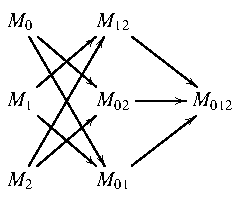
\includegraphics[width=0.54\textwidth]{figures/Fig_102_PDF194_Book182.pdf}
  \caption{三开覆盖的 Čech 复形（原书 p.182）}
  \label{fig:cech-complex-p2}
\end{figure}

根据单项式中负次幂变量的个数，共有四种情形。每出现一个负幂变量 $X_i$，就要删去所有下标中不含 $i$ 的 $M$ 项。各情形所得子复形及其上同调如下图所示：
\begin{figure}[H]\centering
  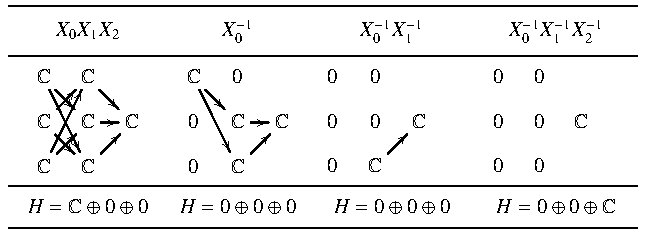
\includegraphics[width=0.96\textwidth]{figures/Fig_103_PDF194_Book182.pdf}
  \caption{按负次幂单项式分解 Čech 复形（原书 p.182）}
  \label{fig:cech-monomial-summands}
\end{figure}
由此可得
\[
  H^i_{\check C}(\mathcal O(k),\mathcal U)=
  \begin{cases}
    R_k, & i=0,\\
    0, & i=1,\\
    \left\langle X_0^{-r}X_1^{-s}X_2^{-t}\ \middle|\ 
    r,s,t\ge1,\ k=-r-s-t\right\rangle, & i=2.
  \end{cases}
\]
\end{example}

\begin{note}\label{note:projective-space-cohomology-range}
\textbf{注 7.21.} 只有 $k\ge0$ 时 $H^0$ 才可能非零，只有 $k\le-3$ 时 $H^2$ 才可能非零。对 $i\ne0,2$，上同调均为零。
\end{note}

\begin{definition}{局部自由层}{locally-free-sheaf}
$X$ 上的局部自由层\index{jubuziyouceng@局部自由层|hyperpage}是一个拟相干层 $\mathcal F$，并且存在一个仿射覆盖 $\mathcal U=\{U_i\mid i\in I\}$，使每个 $\mathcal F(U_i)$ 都是 $\mathcal O(U_i)$-自由模。
\end{definition}

簇上的局部自由相干层是向量丛的代数对应物。事实上，若对某个仿射开集 $U$，$\mathcal F(U)$ 是有限生成自由模，则
\[
  \mathcal F(U)\cong\mathcal O(U)^r,
\]
而对 $U$ 上每个点 $\rho$，纤维为
\[
  \mathcal F(U)_\rho=\mathcal O(U)^r_\rho=\mathbb C^r.
\]
整数 $r$ 称为秩；秩为 $1$ 时，$\mathcal F$ 称为可逆层\index{keniceng@可逆层|hyperpage}。之所以这样命名，是因为可以定义层的张量积，并在仿射开集上令
\[
  (\mathcal M\otimes\mathcal N)(U)
  :=\mathcal M(U)\otimes_{\mathcal O(U)}\mathcal N(U).
\]
在这个运算下，结构层 $\mathcal O$ 是单位元，而可逆层是具有逆元的层；其逆层由
\[
  \mathcal M^{-1}(U):=\operatorname{Hom}_{\mathcal O(U)}(\mathcal M(U),\mathcal O(U))
\]
给出。

\begin{example}[射影空间上的可逆层]
$X=\mathbb P^n$ 上的层 $\mathcal O(k)$ 都是局部自由层。令 $R=\mathbb C[X_0,\ldots,X_n]$，则
\[
  \mathcal O(U_i)=\mathbb C\left[\frac{X_0}{X_i},\ldots,\frac{X_n}{X_i}\right],
\]
并且
\[
  \mathcal O(k)(U_i)=R[X_i^{-1}]_k
  =X_i^k\mathbb C\left[\frac{X_0}{X_i},\ldots,\frac{X_n}{X_i}\right].
\]
因此，$\mathcal O(k)(U_i)$ 是秩为 $1$ 的自由 $\mathcal O(U_i)$-模。
\end{example}

\begin{example}[局部自由但非自由的模]
若 $X=V(R)$ 是仿射簇，则相干层局部自由，当且仅当它对应于一个投射模。这是 Serre--Swan 定理的代数几何版本\bookcite{222}；证明见\bookcite[Tag 00NV]{230}。下面用一个局部自由但非自由的模说明这一点。

取
\[
  R=\mathbb C[X,Y]/(Y^2-X^3+X),
\]
它给出嵌入于 $\mathbb A^2$ 的一条仿射椭圆曲线。模 $\mathcal F=RX+RY$ 不是自由模；但是对开覆盖 $X=U_X\cup U_{X^2-1}$，有
\[
\begin{aligned}
  \mathcal F(U_X)
    &=R[X^{-1}]X+R[X^{-1}]Y=R[X^{-1}],\\
  \mathcal F(U_{X^2-1})
    &=R[(X^2-1)^{-1}]X+R[(X^2-1)^{-1}]Y\\
    &=R[(X^2-1)^{-1}]Y\cong R[(X^2-1)^{-1}].
\end{aligned}
\]
故 $\mathcal F$ 是秩为 $1$ 的局部自由层。更一般地，这条曲线上任意一点所对应的极大理想 $\mathfrak p\subset R$ 都给出秩为 $1$ 的局部自由层，因为总能找到一个开覆盖，使 $\mathfrak p$ 在每个开片上成为主理想。下一节将进一步讨论这一点。
\end{example}

\begin{example}[除子所确定的层]\label{ex:divisor-sheaf}
设 $h(X,Y,Z)$ 是齐次多项式，且 $R=\mathbb C[X,Y,Z]/(h)$ 定义射影平面 $\mathbb P^2$ 中的一条光滑曲线 $X=\mathbb P(R)$。除子是 $X$ 中点的一个整系数组合：
\[
  D=a_1P_1+\cdots+a_kP_k.
\]
每个除子都定义一个层 $\mathcal O(D)$。它在仿射开集 $U$ 上的局部截面，是在每个 $P_i\in U$ 处阶数至少为 $-a_i$ 的有理函数：
\[
  \mathcal O(D)(U)=\left\{\frac fg\ \middle|\ f,g\in\mathcal O(U),\quad
  \operatorname{ord}_{P_i}(f)-\operatorname{ord}_{P_i}(g)\ge -a_i\text{ 对所有 }P_i\in U\right\}.
\]
（回忆：若 $\mathfrak p\subset\mathcal O(U)$ 是对应于点 $P$ 的极大理想，则 $\operatorname{ord}_{P}(f)$ 是满足 $f\in\mathfrak p^n$ 的最大指数 $n$。）与上一个例子类似，这些层都是秩为 $1$ 的局部自由层，也称线丛。线丛 $\mathcal O(D)$ 的次数定义为 $\sum_i a_i$。
\end{example}

给定簇 $(X,\mathcal O)$ 上的两个拟相干层 $\mathcal M,\mathcal N$，定义 Hom 层
\[
  \operatorname{Hom}(\mathcal M,\mathcal N)(U_i)
  :=\operatorname{Hom}_{\mathcal O(U_i)}(\mathcal M(U_i),\mathcal N(U_i)).
\]
这些 Hom 层可用来定义一个以层为态射对象的富集范畴\index{cengzhifanchou@层值范畴|hyperpage} $\mathrm{QCoh}\,X$，其对象是所有相干层，态射空间为相应的 Hom 层。该范畴有全子范畴 $\mathrm{Coh}\,X$ 和 $\mathrm{Vect}\,X$，分别由所有相干层与所有局部自由相干层组成。
% [Tutor Note: 原文称 $\mathrm{QCoh}\,X$ 的对象是“所有相干层”，但按记号 $\mathrm{QCoh}$ 取的应是所有拟相干层，相干层只构成其全子范畴 $\mathrm{Coh}\,X$（这正是下一句所说的全子范畴）；原书此处为笔误，勿据此记忆。]

若取一个开覆盖 $\mathcal U$，则可通过 Čech 复形构造一个 dg-范畴 $\mathrm{Vect}^{\bullet}(X;\mathcal U)$。它与 $\mathrm{Vect}\,X$ 有相同对象，而 Hom 空间为
\[
  \mathrm{Vect}^{\bullet}(X;\mathcal U)(\mathcal M,\mathcal N)
  :=C^\bullet_{\check C}\bigl(\operatorname{Hom}(\mathcal M,\mathcal N);\mathcal U\bigr).
\]
乘积使用杯积。若
\[
  f\in C^k_{\check C}(\operatorname{Hom}(\mathcal N,\mathcal P);\mathcal U),\qquad
  g\in C^\ell_{\check C}(\operatorname{Hom}(\mathcal M,\mathcal N);\mathcal U),
\]
则令
\[
  (f\smile g)_{i_0\cdots i_{k+\ell}}
  =f_{i_0\cdots i_k}|_{U_{i_0\cdots i_{k+\ell}}}
   \circ g_{i_k\cdots i_{k+\ell}}|_{U_{i_0\cdots i_{k+\ell}}}.
\]

\begin{lemma}{仿射覆盖改变下的拟等价}{vector-sheaf-cover-independence}
不同仿射覆盖给出拟等价的 $A_\infty$ 范畴 $\mathrm{Vect}^{\bullet}(X;\mathcal U)$ 与 $\mathrm{Vect}^{\bullet}(X;\mathcal U')$：
\[
  \mathrm{Vect}^{\bullet}(X;\mathcal U)\cong_\infty
  \mathrm{Vect}^{\bullet}(X;\mathcal U').
\]
\end{lemma}
\begin{proof}[证明思路]
证明与 Čech 上同调不依赖仿射覆盖的论证类似：由覆盖细化得到的拟同构与杯积相容。
\end{proof}

\begin{definition}{完美复形范畴}{perfect-complexes-variety}
$X$ 上向量丛完美复形\index{xiangliangcongwanmeifuxingfanchou@向量丛完美复形范畴|hyperpage}的范畴，定义为局部自由层 dg-范畴的导出范畴：
\[
  \mathrm{Perf}^{\bullet}X:=D\mathrm{Vect}^{\bullet}(X;\mathcal U).
\]
\end{definition}

\begin{example}[仿射簇上的完美复形]
若 $X=V(R)$ 是仿射簇，则局部自由层对应于 $R$ 的有限生成投射模。此外，可以取 $\mathcal U=\{V(R)\}$ 作为 $X$ 自身的仿射覆盖，此时 Čech 复形集中在次数 $0$。若投射 $R$-模 $P,Q$ 对应于层 $\mathcal P,\mathcal Q$，则
\[
  \mathrm{Vect}^{\bullet}(X;\mathcal U)(\mathcal P,\mathcal Q)
  =\operatorname{Hom}_R(P,Q).
\]
由此得到 $A_\infty$ 范畴等价
\[
  \mathrm{Vect}^{\bullet}(X;\mathcal U)\cong_\infty
  \mathrm{Proj}^{\bullet}R=\mathrm{SplitAdd}\,R,
\]
其中右侧视为集中在次数 $0$ 的 $A_\infty$ 范畴。取导出范畴后可得
\[
  \mathrm{Perf}^{\bullet}X\cong_\infty D\mathrm{Proj}^{\bullet}R=D^\pi R.
\]
因此 $R$ 是 $\mathrm{Perf}^{\bullet}X$ 的分裂生成元。
\end{example}

\begin{example}[射影平面上的 Beilinson 箭图]\label{ex:beilinson-quiver}
考察 $X=\mathbb P^2$，令 $R=\mathbb C[X_0,X_1,X_2]$。由于 $\mathcal O(k)$ 都是局部自由层，它们是 $\mathrm{Vect}\,X$ 中的对象，而且
\[
  \operatorname{Hom}(\mathcal O(k),\mathcal O(\ell))=\mathcal O(\ell-k).
\]
由例\ref{ex:projective-space-cohomology}中的计算可知，当 $\ell\ge k$ 时，
\[
  \mathrm{Perf}^{\bullet}X(\mathcal O(k),\mathcal O(\ell))=R_{\ell-k}
\]
集中在次数 $0$；当 $\ell-3<k<\ell$ 时，
\[
  \mathrm{Perf}^{\bullet}X(\mathcal O(k),\mathcal O(\ell))=0.
\]
取对象 $\mathcal O,\mathcal O(1),\mathcal O(2)$，可见它们之间只有次数为 $0$ 的态射，而且
\[
  \operatorname{End}_{\mathrm{Perf}^{\bullet}X}
  (\mathcal O\oplus\mathcal O(1)\oplus\mathcal O(2))
  =\begin{pmatrix}
    \mathbb C&R_1&R_2\\
    0&\mathbb C&R_1\\
    0&0&\mathbb C
  \end{pmatrix}=:B.
\]
这个代数还可以写成如下箭图及关系：
\begin{figure}[H]\centering
  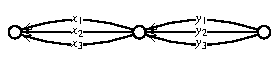
\includegraphics[width=0.52\textwidth]{figures/Fig_104_PDF197_Book185.pdf}
  \caption{Beilinson 箭图（原书 p.185）}
  \label{fig:beilinson-quiver}
\end{figure}
其中关系为 $x_i y_j=x_jy_i$。Beilinson\bookcite{26} 的著名定理说明，这三个对象生成 $\mathrm{Perf}^{\bullet}X$。因此，这个带关系的箭图称为 Beilinson 箭图\index{beilinsonjiantu@Beilinson 箭图|hyperpage}：
\[
  \mathrm{Perf}^{\bullet}X\cong_\infty
  \langle\mathcal O,\mathcal O(1),\mathcal O(2)\rangle
  \cong_\infty DB^{\bullet}.
\]
\end{example}

\subsection{光滑性}\label{subsec:smoothness}
若 $X=V(R)$ 是仿射簇，我们已经看到
\[
  \mathrm{Perf}^{\bullet}X=D\mathrm{Proj}^{\bullet}R
\]
是有界投射 $R$-模复形所成 dg-范畴 $\mathrm{TwSplitAdd}\,R$ 的极小模型。由于 $\mathrm{SplitAdd}\,R\subset\mathrm{Mod}^{\bullet}R$，有包含关系
\[
  \mathrm{Perf}^{\bullet}X\subset D\mathrm{Mod}^{\bullet}R.
\]
反过来，我们知道任意有限生成 $R$-模 $M$ 都有一个投射分解。这给出一个与 $M$ 拟同构的投射 $R$-模复形；遗憾的是，该复形未必有界，因而未必属于 $\mathrm{TwSplitAdd}\,R$。

\begin{example}[两条三次曲线]
考察两条三次曲线。
\begin{itemize}
  \item 令 $R=\mathbb C[X,Y]/(Y^2-X^3-X^2)$，并令 $S=R/(X,Y)$ 为简单模。它有如下自由分解：
  \[
  \cdots\longrightarrow R^2
  \xrightarrow{\left(\begin{smallmatrix}-X^2-X&-Y\\Y&X\end{smallmatrix}\right)}R^2
  \xrightarrow{\left(\begin{smallmatrix}-X&-Y\\Y&X^2+X\end{smallmatrix}\right)}R^2
  \xrightarrow{(Y\quad X)}R\longrightarrow S\longrightarrow0,
  \]
  且末尾这两个映射向左无限重复。由此可算得，对所有 $i>0$，$\operatorname{Ext}^i_R(S,S)=\mathbb C^2$；因此 $S$ 不可能有有界分解。
  \item 令 $R=\mathbb C[X,Y]/(Y^2-X^3+X)$，并令 $S=R/(X,Y)$ 为简单模。它有投射分解
  \[
    0\longrightarrow RX+RY\longrightarrow R\longrightarrow S\longrightarrow0.
  \]
  注意，$RX+RY$ 是投射模，但不是自由模。
\end{itemize}
从几何角度看，这两个模的区别在于：第一种情形中，$S$ 对应于 $V(R)$ 上的奇点；第二种情形中，它对应于一个光滑点。下图画出了相应的两条曲线：
\begin{figure}[H]\centering
  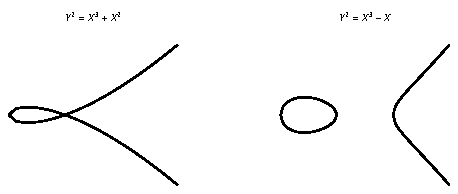
\includegraphics[width=0.66\textwidth]{figures/Fig_105_PDF198_Book186.pdf}
  \caption{奇异与光滑的三次曲线（原书 p.186）}
  \label{fig:singular-smooth-cubics}
\end{figure}
\end{example}

直观地说，光滑点 $\rho\in V(R)$ 是指它附近的空间局部看起来像仿射空间。可以通过完备化使这一说法精确化：令 $\mathfrak p=\ker\rho$，考虑
\[
  \widehat R_{\mathfrak p}=\varprojlim_i R/\mathfrak p^i.
\]
对仿射空间 $\mathbb A^n=V(\mathbb C[X_1,\ldots,X_n])$ 中的零点，有 $\mathfrak p=(X_1,\ldots,X_n)$，因此相应的完备化是形式幂级数环：
\[
  \widehat R_{\mathfrak p}\cong\mathbb C[[X_1,\ldots,X_n]].
\]
一般而言，$\widehat R_{\mathfrak p}$ 总可写成
\[
  \widehat R_{\mathfrak p}\cong\mathbb C[[X_1,\ldots,X_n]]/I,
  \qquad I\subset(X_1,\ldots,X_n)^2.
\]

\begin{definition}{光滑点}{smooth-point}
若点 $\rho\in V(R)$ 关于 $\mathfrak p=\ker\rho$ 的完备化 $\widehat R_{\mathfrak p}$ 同构于形式幂级数环 $\mathbb C[[X_1,\ldots,X_n]]$，则称 $\rho$ 是 $n$ 维光滑点。一般簇 $(X,\mathcal O_X)$ 中的点称为光滑点，如果它在某个仿射开邻域内光滑。簇光滑，当且仅当它的所有点都光滑。
\end{definition}

\begin{note}\label{note:dimension-smooth-points}
\textbf{注 7.32.} 若 $R$ 是整环，则可以证明所有光滑点都具有相同维数；这个维数称为 $V(R)$ 的维数。一般簇称为 $n$ 维的，如果它可由 $n$ 维仿射簇覆盖。
\end{note}

\begin{example}[椭圆曲线的局部完备化]
回到前面两条椭圆曲线。
\begin{itemize}
  \item 若 $R=\mathbb C[X,Y]/(Y^2-X^3+X)$，则零点处的形式完备化为
  \[
    \widehat R_{\mathfrak p}=\mathbb C[[X,Y]]/(Y^2-X^3+X).
  \]
  在该环中，$X=X^3-Y^2$，从而
  \[
    X=X^3-Y^2=(X^3-Y^2)^3-Y^2
      =((X^3-Y^2)^3-Y^2)^3-Y^2=\cdots=f(Y).
  \]
  展开后，含有 $X$ 的项次数会越来越高；极限中得到一个形式幂级数 $X=f(Y)$，所以 $\widehat R_{\mathfrak p}=\mathbb C[[Y]]$。
  \item 若 $R=\mathbb C[X,Y]/(Y^2-X^3-X^2)$，则零点处的形式完备化为
  \[
    \widehat R_{\mathfrak p}=\mathbb C[[X,Y]]/(Y^2-X^3-X^2).
  \]
  这个环不是形式幂级数环，因为它有零因子：$Y\pm X\sqrt{1+X}$ 的形式幂级数展开给出零因子分解。
\end{itemize}
\end{example}

\begin{theorem}{局部光滑性判据}{local-smoothness-criterion}
设 $R$ 是仿射整环，$X=V(R)$，$\rho\in X$ 是对应于简单 $R$-模 $S$ 的点。下列命题等价：
\begin{enumerate}[label=(\roman*)]
  \item $\rho$ 是 $n$ 维光滑点；
  \item $\operatorname{Ext}^{\bullet}_R(S,S)\cong\bigwedge^{\bullet}\mathbb C^n$；
  \item $S$ 有长度为 $n$ 的有限生成投射分解。
\end{enumerate}
\end{theorem}
\begin{proof}[证明思路]
这些等价关系来自一个事实：Ext 群和分解可以局部计算，且
\[
  \operatorname{Ext}^{\bullet}_R(S,S)
  =\operatorname{Ext}^{\bullet}_{R_{\mathfrak p}}(S,S)
  \cong\bigwedge^{\bullet}\mathbb C^n.
\]
更多信息见\bookcite[第 19 章]{74}。
\end{proof}

命题 (iii) 可以用范畴语言改述：点光滑，当且仅当 $S$ 在 $\mathrm{Perf}^{\bullet}X\subset D\mathrm{Mod}^{\bullet}R$ 中与某个对象等价。这个局部观察有一个漂亮的整体版本。

\begin{theorem}{整体光滑性判据：仿射情形}{global-smoothness-affine}
设 $R$ 是仿射整环，$X=V(R)$。下列命题等价：
\begin{enumerate}[label=(\roman*)]
  \item 簇 $X$ 光滑；
  \item 包含 $\mathrm{Perf}^{\bullet}X\subset D\mathrm{Mod}^{\bullet}R$ 是等价；
  \item $D\mathrm{MOD}^{\bullet}R$ 中的 Hom 空间次数有界，即当 $|i|\gg0$ 时，对所有 $M,N$ 都有 $D\mathrm{MOD}^{i}R(M,N)=0$。
\end{enumerate}
\end{theorem}
\begin{proof}[证明思路]
代数几何中的标准事实是：$V(R)$ 为 $n$ 维光滑簇\index{guanghuacu@光滑簇|hyperpage}，当且仅当每个 $R$-模 $M$ 都有长度至多为 $n$ 的投射分解\bookcite[\href{https://stacks.math.columbia.edu/tag/065U}{Tag 065U}]{230}。若 $M$ 有限生成，该分解也可取为有限生成的，因而每个有限生成模都属于 $\mathrm{Perf}^{\bullet}X$。

对任意模，这意味着当 $i>n$ 或 $i<0$ 时，
\[
  \mathrm{MOD}^{i}R(M,N)=\operatorname{Ext}^{i}_R(M,N)=0.
\]
允许扭曲复形后，这些次数可以整体平移有限距离；但每个扭曲复形只有有限个直和项，所以 $\mathrm{Tw}\,\mathrm{MOD}^{\bullet}R$ 与 $D\mathrm{MOD}^{\bullet}R$ 中的 Hom 空间次数仍然有界。
\end{proof}

到目前为止，我们只考察了仿射簇。若要把上述结果推广到一般簇，就需要为 $D\mathrm{Mod}^{\bullet}R$ 和 $D\mathrm{MOD}^{\bullet}R$ 找到合适的对应物。回忆第二章：我们通过以自由分解替换每个模，构造了 $\mathrm{Mod}^{\bullet}R$ 这一 $A_\infty$ 范畴。类似地，这里应当用局部自由层的分解来替换每个相干层。

\begin{definition}{层的复形与局部自由分解}{complex-of-sheaves}
$X$ 上的层复形是一个图表
\[
  P^{\bullet}=\cdots\longrightarrow\mathcal F^{-1}
  \xrightarrow{d^{-1}}\mathcal F^0
  \xrightarrow{d^0}\mathcal F^1
  \xrightarrow{d^1}\mathcal F^2\longrightarrow\cdots,
\]
其中 $d^i\in\operatorname{Hom}(\mathcal F^i,\mathcal F^{i+1})(X)$，且对每个仿射开集 $U\subset X$，限制 $P^{\bullet}(U)$ 都是 $\mathcal O(U)$-模复形。若对每个仿射开集 $U$，$P^{\bullet}(U)$ 都是 $\mathcal M(U)$ 的投射分解，则称 $P^{\bullet}$ 是层 $\mathcal M$ 的局部自由分解。
\end{definition}

若 $P^{\bullet},Q^{\bullet}$ 分别是层 $\mathcal M,\mathcal N$ 的分解，就像前面一样，可以定义它们之间的 Hom 层 $\operatorname{Hom}(P^{\bullet},Q^{\bullet})$。对每个仿射开集 $U$，$\operatorname{Hom}(P^{\bullet},Q^{\bullet})(U)$ 是一个复形，其微分由 $P^{\bullet}$ 和 $Q^{\bullet}$ 的微分诱导。取该 Hom 层的 Čech 复形：
\[
  C^\bullet_{\check C}(\operatorname{Hom}(P^{\bullet},Q^{\bullet});\mathcal U)
  :=\bigoplus_{k,\ell}\bigoplus_{i_1,\ldots,i_k}
  \operatorname{Hom}^{\ell}(P^{\bullet},Q^{\bullet})(U_{i_1\cdots i_k}).
\]
这个双复形带有两个微分：Čech 微分 $d_C$ 提高 $k$ 次数，Hom 微分 $d_H$ 提高 $\ell$ 次数。二者反交换，所以总微分
\[
  d_T=d_C+d_H
\]
是关于 $k+\ell$ 次数的微分，因为
\[
  d_T^2=d_C^2+d_Cd_H+d_Hd_C+d_H^2=0.
\]
不同的局部自由分解和仿射覆盖给出拟同构的复形；其零次上同调是 $\mathcal M$ 与 $\mathcal N$ 的 Hom 层的整体截面：
\[
  H^0C^\bullet_{\check C}(\operatorname{Hom}(P^{\bullet},Q^{\bullet});\mathcal U)
  =\operatorname{Hom}(\mathcal M,\mathcal N)(X).
\]

\begin{definition}{层的导出范畴}{derived-categories-of-sheaves}
以拟相干层的局部自由分解为对象、以上述 Čech 复形为 Hom 空间的范畴，在总微分下构成一个 dg-范畴。记其极小模型为 $\mathrm{Coh}^{\bullet}X$（$\mathrm{QCoh}^{\bullet}X$），并记其导出版本为 $D\mathrm{Coh}^{\bullet}X$（$D\mathrm{QCoh}^{\bullet}X$）。后者称为（拟）相干层的有界导出范畴\index{xianggancengdeyoujiedaochufanchou@相干层的有界导出范畴|hyperpage}。
\end{definition}

由于 $\mathrm{Vect}^{\bullet}X$ 中每个对象都是自身的分解，存在包含
\[
  \mathrm{Vect}^{\bullet}X\subset\mathrm{Coh}^{\bullet}X
  \subset\mathrm{QCoh}^{\bullet}X.
\]
取导出范畴后得到以下两列 $A_\infty$ 范畴：
\[
\begin{array}{ll}
  \text{仿射情形:}&\mathrm{Perf}^{\bullet}X\subset D\mathrm{Mod}^{\bullet}R
    \subset D\mathrm{MOD}^{\bullet}R,\\
  \text{一般情形:}&\mathrm{Perf}^{\bullet}X\subset D\mathrm{Coh}^{\bullet}X
    \subset D\mathrm{QCoh}^{\bullet}X.
\end{array}
\]
有了这些定义，就可以把前面的定理推广到一般情形。

\begin{theorem}{整体光滑性判据：一般情形}{global-smoothness-general}
设 $X$ 是一个簇。下列命题等价：
\begin{enumerate}[label=(\roman*)]
  \item 簇 $X$ 光滑；
  \item 包含 $\mathrm{Perf}^{\bullet}X\subset D\mathrm{Coh}^{\bullet}X$ 是等价；
  \item $D\mathrm{QCoh}^{\bullet}X$ 中的 Hom 空间次数有界。
\end{enumerate}
\end{theorem}
% [Tutor Note: 光滑性判据的几何含义：$\mathrm{Perf}^{\bullet}X$ 是“由向量丛生成的有限复形”，$D\mathrm{Coh}^{\bullet}X$ 是全体有界复形；$X$ 光滑时二者相等（每个相干层都有有限局部自由分解），$X$ 有奇点时商 $D^b\mathrm{Coh}X/\mathrm{Perf}X$ 非零，它只探测奇点，这正是 §7.2.5 的奇点范畴 $\operatorname{Sing}X$。]

\begin{note}\label{note:projective-derived-hom-finite}
\textbf{注 7.39.} 若进一步假设 $X$ 是射影簇，则 $D\mathrm{Coh}^{\bullet}X$ 中的 Hom 空间不仅次数有界，而且有限维。换言之，$D\mathrm{Coh}^{\bullet}X$ 是 Hom 有限的 $A_\infty$ 范畴。
\end{note}

光滑簇自然带有一组局部自由层，它们是微分几何中相应对象的代数类比。

\begin{definition}{切层、余切层与典范层}{tangent-cotangent-canonical-sheaves}
设 $(X,\mathcal O)$ 是一个簇。
\begin{itemize}
  \item 切层\index{qieceng@切层|hyperpage} $T$ 定义为 $X$ 上的导子层：
  \[
    T(U):=\operatorname{Der}(\mathcal O(U))
    =\{\delta\colon\mathcal O(U)\to\mathcal O(U)\mid
    \delta(uv)=\delta(u)v+u\delta(v)\}.
  \]
  \item 余切层\index{yuqieceng@余切层|hyperpage} $T^*$ 定义为切层的对偶：
  \[
    T^*(U):=\operatorname{Hom}_{\mathcal O(U)}(T(U),\mathcal O(U)).
  \]
  对 $f,g\in\mathcal O(U)$，表达式 $f\,dg$ 可视为 $T^*(U)$ 中的元素，具体由 $f\,dg(\delta)=f\delta(g)$ 给出。
  \item 微分 $k$-形式层 $\Omega^\bullet$ 是余切层关于结构层的外代数：
  \[
    \Omega^\bullet(U):=\bigwedge^\bullet T^*(U)
    =\frac{\displaystyle\bigoplus_{n=0}^{\infty}T^*(U)^{\otimes n}}
      {\langle u\otimes v-v\otimes u\mid u,v\in T^*(U)\rangle}.
  \]
  \item 典范层\index{dianfanceng@典范层|hyperpage}是最高次微分形式层\index{weifenxingshiceng@微分形式层|hyperpage}：
  \[
    K(U):=\Omega^n(U),\qquad n=\dim X.
  \]
\end{itemize}
\end{definition}

\begin{theorem}{光滑簇上的向量丛}{vector-sheaves-smooth}
若 $(X,\mathcal O)$ 光滑，则 $T,T^*$ 和 $\Omega^k$ 都是局部自由层，且 $K$ 是线丛。
\end{theorem}
\begin{proof}[证明思路]
参见\bookcite[\href{https://stacks.math.columbia.edu/tag/05D4}{Tag 05D4}]{230}。
\end{proof}

\begin{example}[射影空间的典范丛]
若 $X=\mathbb P^1$，则在 $U_0$ 上可用坐标 $\xi=X/Y$ 局部写出导子 $f(\xi)\,\frac d{d\xi}$。在 $U_1$ 上令 $\eta=Y/X=\xi^{-1}$，则
\[
  f(\xi)\frac d{d\xi}
  =-f(\eta^{-1})\eta^2\frac d{d\eta}.
\]
因此，当 $f$ 的次数不超过 $2$ 时，该导子可在整体上定义，故 $T(X)=\mathbb C^3$，且 $T=\mathcal O(2)$。另一方面，由 $d\xi=-\eta^{-2}d\eta$ 可知
\[
  T^*=\Omega^1=K=\mathcal O(-2).
\]
一般地，可以证明 $\mathbb P^n$ 的典范丛为 $K=\mathcal O(-n-1)$，因为
\[
  d\xi_{10}\wedge\cdots\wedge d\xi_{n0}
  =\pm\xi_{01}^{-n-1}
  d\xi_{01}\wedge\cdots\wedge d\xi_{n1}.
\]
\end{example}

\section{其他几何对象}\label{sec:other-geometrical-objects}
\takeaway{支撑层、概形、非交换簇与栈把导出范畴推广到更广的对象；Landau--Ginzburg 模型 $(X,W)$ 的矩阵分解由 $d_0d_1=d_1d_0=W$ 刻画，Knörrer 周期性、Dyckerhoff 生成定理与 Buchweitz 定理把 $\mathrm{MF}^{\pm}(R,W)$ 与 $W^{-1}(0)$ 的奇点范畴联系起来。}
本节考察代数几何中的其他一些对象。与簇类似，我们也可以构造仿射版本和非仿射版本；后者由粘合仿射片得到，但这里不详细展开。

\subsection{支撑}\label{subsec:support}
设 $X$ 是仿射簇，$I$ 是 $R=\mathcal O(X)$ 中的理想，并假设 $R/I$ 是仿射整环。则有自然嵌入
\[
  Y=V(R/I)\hookrightarrow X,
\]
其像是 $X$ 的闭子集。若 $M$ 是 $R/I$-模，也可以把它看作 $R$-模。由此得到嵌入
\[
  \mathrm{Coh}\,Y\subset\mathrm{Coh}\,X,
\]
其中右侧的子范畴由所有支撑在 $Y$ 上的 $X$-层组成。

作为普通范畴，这是一个全忠实嵌入；但加入额外的 $A_\infty$ 结构后，情形便不再如此。事实上，若 $Y=\{p\}$ 是 $X=\mathbb A^1$ 中的一个点，则简单模 $S_p$ 作为 $\mathcal O(Y)$-模的 $A_\infty$ 自同态环为
\[
  \operatorname{Ext}^{\bullet}_{\mathbb C}(S_p,S_p)=\mathbb C,
\]
而作为 $\mathcal O(X)$-模时则为
\[
  \operatorname{Ext}^{\bullet}_{\mathbb C[X]}(S_p,S_p)
  =\mathbb C\langle\xi\rangle/(\xi^2).
\]

\begin{definition}{支撑在闭子簇上的导出范畴}{derived-category-support}
$X$ 上支撑在 $Y$ 上的相干层导出范畴记为 $D\mathrm{Coh}^{\bullet}_Y(X)$；它是 $D\mathrm{Coh}^{\bullet}(X)$ 的 $A_\infty$ 子范畴，由把 $Y$ 上的层视为 $X$ 上的层后所生成。
\end{definition}

\begin{example}[光滑点的无穷小邻域]
若 $Y=\{p\}$ 是簇 $X$ 中一个 $n$ 维光滑点，则 $D\mathrm{Coh}^{\bullet}_Y(X)$ 由点层 $S_p$ 生成。这意味着 $D\mathrm{Coh}^{\bullet}_Y(X)$ 包含 $S_p$ 的自扩张；这些扩张是 $\mathrm{Coh}\,X$ 中的层，却不属于 $\mathrm{Coh}\,Y\subset\mathrm{Coh}\,X$。

由于 $S_p$ 在 $D\mathrm{Coh}^{\bullet}(X)$ 中的自同态环是外代数 $\Lambda^\bullet_n$，我们有
\[
  D\mathrm{Coh}^{\bullet}_Y(X)\cong_\infty D\Lambda^\bullet_n.
\]
这个范畴等价于 $D\mathrm{mod}\,\mathbb C[[X_1,\ldots,X_n]]$，所以它只看见 $Y$ 在 $X$ 中的无穷小邻域。
\end{example}

\begin{note}\label{note:singular-support-in-smooth-variety}
\textbf{注 7.45.} 一般而言，若 $Y$ 是奇异的而 $X$ 光滑，则 $D\mathrm{Coh}^{\bullet}_Y(X)$ 的表现会比 $D\mathrm{Coh}^{\bullet}(Y)$ 好得多。
\end{note}

\subsection{概形}\label{subsec:schemes}
概形\index{gaixing@概形|hyperpage}是簇的推广，在这种推广中，坐标环允许是任意交换环 $R$。与 $R$ 对应的空间记作 $\operatorname{Spec}(R)$，其点由 $R$ 的所有素理想组成。$\operatorname{Spec}(R)$ 中的仿射开集具有如下形式：
\[
  U_f=\{\mathfrak p\in\operatorname{Spec}(R)\mid f\notin\mathfrak p\}.
\]
与普通簇类似，可以把 $R$ 变成 $\operatorname{Spec}(R)$ 上的环层 $\mathcal O$，令
\[
  \mathcal O(U_f)=R[f^{-1}].
\]
与 $R$ 对应的概形是带环层空间 $X=(\operatorname{Spec}(R),\mathcal O)$，并且可以按通常方式定义（拟）相干层。

若 $R$ 是仿射环，则可将 $V(R)$ 嵌入 $\operatorname{Spec}(R)$：把表示 $\rho\colon R\to\mathbb C$ 映到极大理想 $\ker\rho$。虽然 $\operatorname{Spec}(R)$ 通常比 $V(R)$ 含有更多点，但这两个拓扑空间的形态十分相似。特别地，相应的开集范畴等价：
\[
  \mathrm{Open}_{V(R)}\simeq\mathrm{Open}_{\operatorname{Spec}(R)}.
\]
因此，概形版本的 $\mathrm{Coh}^{\bullet}X$、$\mathrm{QCoh}^{\bullet}X$ 与 $\mathrm{Perf}^{\bullet}X$ 和簇版本相同，并分别等价于 $\mathrm{MOD}^{\bullet}R$、$\mathrm{Mod}^{\bullet}R$ 与 $D\mathrm{Proj}^{\bullet}R$。
% [Tutor Note: 这句的对应顺序按本书记号是反的：$MOD^{\bullet}R$ 为全部（右）模、$Mod^{\bullet}R$ 为有限生成模（见第 1 章 §1.5 的约定），故与仿射簇的对应应为 Coh$\leftrightarrow$Mod、QCoh$\leftrightarrow$MOD。原书此处把两个记号对调，对照 §7.1.4 末尾的范畴塔 $\mathrm{Coh}^{\bullet}X\subset\mathrm{QCoh}^{\bullet}X$、$D\mathrm{Mod}^{\bullet}R\subset D\mathrm{MOD}^{\bullet}R$ 即可确认。]

\begin{example}[一般点]
若 $R=\mathbb C[X]$，则 $\operatorname{Spec}(R)$ 比 $V(R)$ 多一个点，它对应素理想 $(0)$。由于 $f\notin(0)$，这个点属于每个 $U_f$，因而位于任意点的闭包中。这个点称为 $\operatorname{Spec}(R)$ 的一般点。
\end{example}

\begin{example}[胖点]
若 $R=\mathbb C[X]/(X^n)$，则 $\operatorname{Spec}(R)$ 只有一个点，即素理想 $\mathfrak p=(X)$。当 $n=1$ 时，该概形就是由一个点构成的仿射簇；当 $n>1$ 时，概形仍只有一个点，但该点附近的函数环更大，是 $R$ 而非 $\mathbb C$。因此它称为胖点\index{pangdian@胖点|hyperpage}。其导出范畴为
\[
  D\mathrm{Coh}^{\bullet}X=D\mathrm{Mod}^{\bullet}\mathbb C[X]/(X^n),
\]
它不等于 $\mathrm{Perf}^{\bullet}\mathbb C[X]/(X^n)$，所以胖点是奇异概形。
\end{example}

概形的更多内容参见\bookcite{109,184,72}。

\subsection{非交换簇}\label{subsec:noncommutative-varieties}
我们还可以尝试把视角推广到非交换环。理想情况下，希望把 $\mathrm{Mod}^{\bullet}R$ 或 $\mathrm{MOD}^{\bullet}R$ 看成某个拓扑空间上的层范畴。一般而言，这很难做到，因为“点”可能有不同的合理定义，例如素理想、极大理想、简单表示或一维表示；每种定义都有各自的缺点。通常更好的做法是完全不考虑空间，只研究范畴 $\mathrm{Mod}^{\bullet}R$、$\mathrm{MOD}^{\bullet}R$ 及其导出版本 $D\mathrm{Mod}^{\bullet}R$、$D\mathrm{MOD}^{\bullet}R$。

\begin{example}[射影空间的非交换仿射模型]
在某些情形下，射影簇可以看作仿射非交换簇。由第 4.4.2 节可知
\[
  D\mathrm{Coh}^{\bullet}\mathbb P^1
  \cong_\infty D\mathrm{mod}^{\bullet}Q
  =D\mathrm{Mod}^{\bullet}Q,
\]
其中 $Q$ 是克罗内克箭图：
\begin{figure}[H]\centering
  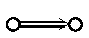
\includegraphics[width=0.30\textwidth]{figures/Fig_106_PDF204_Book192.pdf}
  \caption{克罗内克箭图（原书 p.192）}
  \label{fig:kronecker-quiver-b-side}
\end{figure}
这是因为我们找到了 $D\mathrm{Coh}^{\bullet}\mathbb P^1$ 的一个分裂生成元，其自同态环是 $Q$ 的路径代数。类似地，由例\ref{ex:beilinson-quiver}可得
\[
  D\mathrm{Coh}^{\bullet}\mathbb P^2
  \cong_\infty\mathrm{Perf}^{\bullet}\mathbb P^2
  \cong_\infty D\mathrm{Mod}^{\bullet}B,
\]
其中 $B$ 是由 Beilinson 箭图及其关系给出的路径代数。
\end{example}

若把非交换代数 $A$ 视为某个非交换簇上的函数环，把它的模视为拟相干层，就可以把几何概念转移到非交换情形。与交换簇类似，这里有三个值得关注的范畴：$D\mathrm{MOD}^{\bullet}A$ 对应 $D\mathrm{QCoh}^{\bullet}X$；有限生成模组成的 $D\mathrm{Mod}^{\bullet}A$ 对应 $D\mathrm{Coh}^{\bullet}X$；而
\[
  \mathrm{Perf}^{\bullet}A:=D\mathrm{Proj}^{\bullet}A
\]
对应 $\mathrm{Perf}^{\bullet}X$。不过，若 $A$ 不是 Noether 环，则 $D\mathrm{Mod}^{\bullet}A$ 的性质不佳，因为 $\mathrm{Mod}\,A$ 对取核不封闭。因此，下面假设 $A$ 是 Noether 环。

\begin{definition}{代数的整体维数}{global-dimension-algebra}
代数 $A$ 的（右）整体维数\index{zhengtiweishu@整体维数|hyperpage}，是使得存在 $M,N\in\mathrm{MOD}^{\bullet}A$ 满足 $\operatorname{Ext}^n_A(M,N)\ne0$ 的最大整数 $n$。若不存在这样的最大整数，则称 $A$ 的整体维数为无穷。
\end{definition}

\begin{example}[若干代数的整体维数]
列出一些重要代数的整体维数。
\begin{itemize}
  \item （斜）域的整体维数为 $0$，因为所有模都是自由模。
  \item 光滑 $n$ 维仿射簇的坐标环整体维数为 $n$。
  \item 箭图 $Q$ 的路径代数 $\mathbb C Q$ 的整体维数为 $1$，因为每个模 $M$ 都有如下分解：
  \[
    0\longrightarrow
    \bigoplus_{a\in Q_1}M_{h(a)}\otimes t(a)\mathbb C Q
    \xrightarrow{\ a\otimes t(a)-h(a)\otimes a\ }
    \bigoplus_{v\in Q_0}M_v\otimes v\mathbb C Q
    \longrightarrow M\longrightarrow0.
  \]
  \item 由 Beilinson 箭图及关系给出的路径代数，其整体维数为 $2$。
  \item 注意，整体维数不在导出等价下保持不变。下图所示的两个代数具有相同的导出范畴，但前者整体维数为 $1$，后者为 $2$：
  \begin{figure}[H]\centering
    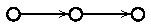
\includegraphics[width=0.33\textwidth]{figures/Fig_107_PDF205_Book193.pdf}\quad
    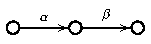
\includegraphics[width=0.37\textwidth]{figures/Fig_108_PDF205_Book193.pdf}
    \caption{导出等价但整体维数不同的代数（原书 p.193）}
    \label{fig:derived-equivalent-global-dimensions}
  \end{figure}
  \item 整体维数有限并不是一个很强的条件：每个没有有向圈的箭图所给出的带关系路径代数，都有有限整体维数。
\end{itemize}
\end{example}

\begin{theorem}{Noether 代数的光滑性判据}{smoothness-noetherian-algebra}
若 $A$ 是 Noether 环且整体维数为 $n$，则
\begin{enumerate}[label=(\roman*)]
  \item $\mathrm{Perf}^{\bullet}A\subset D\mathrm{Mod}^{\bullet}A$ 是等价；
  \item $D\mathrm{MOD}^{\bullet}A$ 中的 Hom 空间次数有界。
\end{enumerate}
\end{theorem}
\begin{proof}[证明思路]
若整体维数为 $n$，则每个模都有长度至多为 $n$ 的投射分解。由于 $A$ 是 Noether 环，这个分解可取为有限生成的，因此属于 $\mathrm{Perf}^{\bullet}A$。另一方面，我们知道模之间的 Hom 空间次数有界，所以对模的扭曲复形取 Hom 空间时，次数仍然有界。
\end{proof}

\begin{note}\label{note:noncommutative-geometry-approaches}
\textbf{注 7.52.} 把几何思想转移到非交换情形时往往不够完美，因此根据研究重点不同，存在多种非交换代数几何路径\bookcite{152,145,226}；这一领域与有限维代数表示论也有许多交叉\bookcite{97,108}。
\end{note}

\subsection{栈}\label{subsec:stacks}
设有限群 $G$ 作用在仿射簇 $X$ 上。我们希望构造一个新簇，使其点对应于 $X$ 中的轨道。为此需要找出新簇的坐标环。$G$ 在原簇上的作用诱导 $G$ 对坐标环 $R=\mathcal O(X)$ 的作用：
\[
  \forall g\in G,\ f\in R,\ x\in X,\qquad
  (g\cdot f)(x):=f(g^{-1}\cdot x).
\]
轨道集上的函数可以看成 $X$ 上在群作用下不变的函数。它们组成一个环
\[
  R^G:=\{f\in R\mid g\cdot f=f\text{ 对所有 }g\in G\},
\]
并定义商簇
\[
  X//G:=V(R^G).
\]
自然嵌入 $R^G\hookrightarrow R$ 诱导投影映射 $\pi\colon X\to X//G$；由于 $G$ 有限，$\pi$ 的纤维恰好是 $G$-轨道。

\begin{definition}{范畴商}{categorical-quotient}
簇 $X//G:=V(R^G)$ 称为范畴商\index{fanchoushang@范畴商|hyperpage}。
\end{definition}

\begin{example}[单位根作用的商]
令 $X=\mathbb A^1$，$G=\mathbb Z_n$，并令 $G$ 通过乘以 $n$ 次单位根作用。此时 $R=\mathbb C[X]$，不变函数正是关于 $X^n$ 的多项式。因此
\[
  \mathcal O(X//G)=\mathbb C[X^n],\qquad X//G\cong\mathbb A^1.
\]
\end{example}

上例表明，不变环并未完全捕捉商的几何结构：在 $X//G\cong\mathbb A^1$ 中，所有点看起来都一样，但商中有一个特殊点，即零轨道。这个轨道只含一个点，其余轨道都含 $\#G$ 个点。为解决这一问题，可以构造一个新的环。

\begin{definition}{叉积（smash product）}{smash-product}
若 $X=V(R)$ 是仿射簇，有限群 $G$ 作用在 $X$ 上，则定义叉积\index{chaji@叉积|hyperpage} $R\star G$ 为由 $R$ 与 $G$ 中元素线性组合组成的环：
\[
  R\star G:=\left\{\sum_i f_i g_i\ \middle|\ f_i\in R,\ g_i\in G\right\},
\]
其乘法满足
\[
  (f_1g_1)(f_2g_2)=\bigl(f_1(g_1\cdot f_2)\bigr)g_1g_2.
\]
\end{definition}

若 $G$ 的作用是忠实的，可以证明叉积 $R\star G$ 的中心等于不变环 $R^G$。叉积是一个非交换 $\mathbb C$-代数，因此可以将它视为一个非交换簇。

\begin{definition}{商栈}{quotient-stack}
商栈\index{shangzhan@商栈|hyperpage} $[X/G]$ 是与叉积 $R\star G$ 对应的非交换簇；按定义，
\begin{align*}
  \mathrm{Perf}^{\bullet}[X/G]&:=\mathrm{Perf}^{\bullet}(R\star G),\\
  D\mathrm{Coh}^{\bullet}[X/G]&:=D\mathrm{Mod}^{\bullet}(R\star G),\\
  D\mathrm{QCoh}^{\bullet}[X/G]&:=D\mathrm{MOD}^{\bullet}(R\star G).
\end{align*}
\end{definition}

\begin{example}[仿射直线的循环群商栈]
令 $X=\mathbb C$，$G=\mathbb Z/n\mathbb Z$，作用为乘以 $n$ 次单位根。由定理~\ref{thm:cyclic-quiver-crossed-product}，商栈对应于有 $n$ 个顶点的循环箭图路径代数：
\begin{figure}[H]\centering
  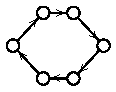
\includegraphics[width=0.28\textwidth]{figures/Fig_109_PDF206_Book194.pdf}
  \caption{循环箭图（原书 p.194）}
  \label{fig:cyclic-quiver-stack}
\end{figure}
\[
  \mathcal O(X)\star G\cong\mathbb C Q.
\]
因此
\[
  D\mathrm{Coh}^{\bullet}[X/G]\cong D\mathrm{Mod}^{\bullet}Q,
  \qquad D\mathrm{Coh}^{\bullet}(X//G)\cong D\mathrm{Mod}^{\bullet}\mathbb C[X],
\]
所以商栈确实与商簇不同。
\end{example}

从几何角度看，商栈通常比范畴商表现得更好。

\begin{example}[平面上的二阶群作用]
令 $G=\mathbb Z/2\mathbb Z\cong\{1,-1\}\cong\langle g\mid g^2=1\rangle$，并令它通过同时乘以 $-1$ 的方式对角作用在 $\mathbb A^2$ 上。$\mathbb C[X,Y]^G$ 由 $\xi=X^2$、$\eta=Y^2$、$\zeta=XY$ 生成，因此
\[
  \mathbb C[X,Y]^G\cong\mathbb C[\xi,\eta,\zeta]/(\xi\eta-\zeta^2).
\]
这表明 $X//G$ 是一个锥，并非光滑簇。另一方面，商栈 $[\mathbb A^2/G]$ 上的相干层可以看成有限生成的 $A$-模，其中
\[
  A=\mathbb C[X,Y]\star G
  =\frac{\mathbb C\langle X,Y,g\rangle}
  {(XY-YX,\ gX+Xg,\ gY+Yg,\ g^2-1)}.
\]
这个代数同构于下图所示带关系的箭图路径代数：
\begin{figure}[H]\centering
  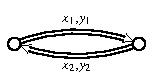
\includegraphics[width=0.43\textwidth]{figures/Fig_110_PDF207_Book195.pdf}
  \caption{商栈代数的箭图及关系（原书 p.195）}
  \label{fig:quotient-stack-quiver}
\end{figure}
其关系为
\[
  \mathcal R=\langle x_1y_2-y_1x_2,\ x_2y_1-y_2x_1\rangle.
\]
每个 $A$-模 $M$ 都有如下形式的投射分解：
\[
  0\longrightarrow M\otimes_{\mathbb CG}A
  \xrightarrow{\binom{-Y}{X}}
  (M\otimes_{\mathbb CG}A)^{\oplus2}
  \xrightarrow{(X\quad Y)}M\otimes_{\mathbb CG}A
  \longrightarrow M\longrightarrow0.
\]
\begin{figure}[H]\centering
  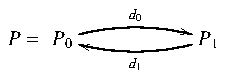
\includegraphics[width=0.62\textwidth]{figures/Fig_111_PDF207_Book195.pdf}
  \caption{叉积代数模的投射分解（原书 p.195）}
  \label{fig:quotient-stack-resolution}
\end{figure}
所以 $A$ 的整体维数为 $2$。由于 $A$ 是 Noether 环，有
\[
  D\mathrm{Coh}^{\bullet}[\mathbb A^2/G]
  \simeq\mathrm{Perf}^{\bullet}[\mathbb A^2/G].
\]
\end{example}

\begin{note}\label{note:stacks-equivariant-sheaves}
\textbf{注 7.59.} 也可以把 $[X/G]$ 上的相干层定义为 $X$ 上的 $G$-等变层。这种方法使我们能够对非仿射簇定义栈商。栈的概念甚至可以推广到不来自群作用商的情形。栈的简要介绍见\bookcite{76,196}。
\end{note}

\subsection{Landau--Ginzburg 模型}\label{subsec:landau-ginzburg-models}
矩阵分解\index{juzhenfenjie@矩阵分解|hyperpage}最初由 Eisenbud 在文献\bookcite{73}中引入，之后被物理学家用于研究某些称为 Landau--Ginzburg 模型\index{landauginzburgmoxing@Landau–Ginzburg 模型|hyperpage}的物理模型。Landau--Ginzburg 模型由一对 $(X,W)$ 组成，其中 $X$ 是一个簇，$W\colon X\to\mathbb C$ 是全纯函数。若 $X$ 是仿射簇，可以把 $W$ 看作 $\mathcal O(X)$ 中的元素；它通常称为势\index{shi@势|hyperpage}。

\begin{definition}{矩阵分解范畴}{matrix-factorization-category}
设 $(R,W)$ 是一对数据，其中 $R$ 是仿射整环，$W\in R$。
\begin{itemize}
  \item $(R,W)$ 的一个矩阵分解是一个图表
  \[
    P=P_0\underset{d_1}{\overset{d_0}{\rightleftarrows}}P_1,
    \qquad d_0d_1=W1_{P_1},\quad d_1d_0=W1_{P_0},
  \]
  其中 $P_0,P_1$ 是有限生成投射模（即 $V(R)$ 上的向量丛）。
  \item 两个矩阵分解 $P,Q$ 之间的态射空间为
  \[
    \bigoplus_{i,j\in\mathbb Z_2}\operatorname{Hom}_R(P_i,Q_j),
  \]
  微分对齐次态射 $f$ 定义为
  \[
    d\begin{pmatrix}f_{00}&f_{01}\\f_{10}&f_{11}\end{pmatrix}
    =\begin{pmatrix}0&d_1\\d_0&0\end{pmatrix}_{Q}
      \begin{pmatrix}f_{00}&f_{01}\\f_{10}&f_{11}\end{pmatrix}
      -\begin{pmatrix}f_{00}&-f_{01}\\-f_{10}&f_{11}\end{pmatrix}
       \begin{pmatrix}0&d_1\\d_0&0\end{pmatrix}_{P}.
  \]
% [Tutor Note: 微分公式右端的第二个矩阵正是 Koszul 符号：记 $\sigma=\operatorname{diag}(1,-1)$，则右端第二个矩阵等于 $\sigma f\sigma=(-1)^{|f|}f$（$f$ 为奇次时四个分量依次变号），故 $d(f)=d_Qf-(-1)^{|f|}fd_P$。漏掉这个符号 $d^2$ 一般不为零，这是矩阵分解 Hom 复形最易出错之处。]
  \item 矩阵分解范畴\index{juzhenfenjiefanchou@矩阵分解范畴|hyperpage} $\mathrm{MF}^{\pm}(R,W)$ 是以上述对象和态射为基础的 dg-范畴的极小模型。
\end{itemize}
\end{definition}

\begin{note}\label{note:matrix-factorizations-curved-algebra}
\textbf{注 7.61.} 若 $R$ 是多项式环，则 Quillen--Suslin 定理\index{quillensuslindingli@Quillen–Suslin 定理|hyperpage}\bookcite{206}说明每个投射 $R$-模都是自由模。结合例~\ref{ex:matrix-factorizations-from-potential}，可以把 $P_i$ 看成 $R^{\oplus k}$，把 $d_i$ 看成系数属于 $R$ 的矩阵。换言之，
\[
  \left(P_0\oplus P_1[1],
  \begin{pmatrix}0&d_1\\d_0&0\end{pmatrix}\right)
\]
是带曲率代数 $R_W$ 上的一个扭曲复形：
\[
  \mathrm{MF}^{\pm}(R,W)=H^0\mathrm{Tw}_{R_W}
  ={}^0\mathrm{D}R_W.
\]
\end{note}

\begin{example}[乘积势 $XY$ 的矩阵分解]
取环 $R=\mathbb C[X,Y]$ 与多项式 $W=XY$。有一个自然的矩阵分解：
\[
  S:=R\underset{Y}{\overset{X}{\rightleftarrows}}R.
\]
\begin{figure}[H]\centering
  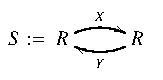
\includegraphics[width=0.23\textwidth]{figures/Fig_112_PDF208_Book196.pdf}
  \caption{$XY$ 的基本矩阵分解（原书 p.196）}
  \label{fig:xy-matrix-factorization}
\end{figure}
我们有 $\operatorname{End}_{\mathrm{MF}^{\pm}}(S,S)=\mathbb C\,1$。事实上，可以证明 $\mathrm{MF}^{\pm}(R,W)$ 由 $S$ 生成，因此它等价于 $D\mathbb C^{\pm}$，即一个点的 $\mathbb Z_2$-分次导出范畴；也就是说，它等价于矩阵分解范畴 $\mathrm{MF}^{\pm}(\mathbb C,0)$。

这并非巧合。一般而言，$\mathrm{MF}^{\pm}(R,W)$ 可用于描述零纤维
\[
  W^{-1}(0)=V(R/(W))
\]
的奇异集。对每个 $p\in W^{-1}(0)\subset\mathbb C^n$，都可以构造一个矩阵分解。设 $R=\mathbb C[X_1,\ldots,X_n]$，$p=0\in W^{-1}(0)$，并写成
\[
  W=\sum_rX_rW_r,
\]
其中 $W_r$ 是多项式。令
\[
  \Omega^{\pm}=R\otimes\bigwedge^\bullet\mathbb C^n
\]
为微分形式空间，并将其视为 $\mathbb Z_2$-分次 $R$-模。定义 $R$-线性映射
\[
  d\omega=\sum_rX_r\,\iota_{\partial_{X_r}}\omega
          +\sum_rW_r\,dX_r\wedge\omega.
\]
注意，$d$ 的第一部分 $\mathbb Z$-次数为 $-1$，因为它把 $\partial_{X_r}$ 插入 $\omega$；第二部分 $\mathbb Z$-次数为 $+1$，因为它把 $\omega$ 与一个 $1$-形式作外积。因此，总微分仅关于 $\mathbb Z_2$ 分次齐次。可以算得 $d^2\omega=W\omega$（另见例 12.13），所以
% [Tutor Note: 直接验证：由 $\iota_{\partial_r}(dX_s\wedge\omega)=\delta_{rs}\omega-dX_s\wedge\iota_{\partial_r}\omega$ 可知，$d^2\omega$ 中“先插入再外乘”与“先外乘再插入”的两组项逐项相消，只剩 $\sum_rX_rW_r\omega=W\omega$。又 $d$ 的两部分 $\mathbb Z$-次数分别为 $-1$ 与 $+1$，故 $d$ 本身并非 $\mathbb Z$-齐次，只在 $\mathbb Z_2$ 分次下齐次——这正是矩阵分解范畴取 $\mathbb Z_2$-分次的来源。]
\[
  M_p=(\Omega^{\pm},d)
\]
是 $W$ 的一个矩阵分解，并且有两个重要性质：
\begin{itemize}
  \item 若选取 $W=\sum_rX_rW'_r$ 的另一种分解，则得到的矩阵分解与原矩阵分解拟同构；
  \item 若某个 $W_r$ 有常数项，则 $(\Omega^{\pm},d)$ 拟等价于零对象。
\end{itemize}
这说明 $M_p$ 只依赖于点 $p$，并且仅当 $p$ 属于 $W^{-1}(0)$ 的奇异集时才非零。记
\[
  \operatorname{Sing}(W)=\{p\in W^{-1}(0)\mid(dW)_p=0\}.
\]
\end{example}

\begin{example}[三条直线的并]
令 $R=\mathbb C[X,Y]$，$W=XY(X-Y)$。有三个显然的矩阵分解：
\[
  S_X:=R\underset{Y(X-Y)}{\overset X{\rightleftarrows}}R,\qquad
  S_Y:=R\underset{X(X-Y)}{\overset Y{\rightleftarrows}}R,\qquad
  S_{X-Y}:=R\underset{XY}{\overset{X-Y}{\rightleftarrows}}R.
\]
\begin{figure}[H]\centering
  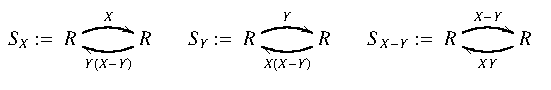
\includegraphics[width=0.73\textwidth]{figures/Fig_113_PDF209_Book197.pdf}
  \caption{$XY(X-Y)$ 的三个基本矩阵分解（原书 p.197）}
  \label{fig:three-line-matrix-factorizations}
\end{figure}
对每个 $Z\in\{X,Y,X-Y\}$，都有
\[
  \operatorname{End}_{\mathrm{MF}}(S_Z,S_Z)=\frac{\mathbb C[U]}{(U^2)},
\]
其中 $U$ 是乘积 $W/Z$ 中的一个因子。任取其中一个因子都可以，因为它们代表同一个上同调类，至多相差一个符号。

另一方面，$\operatorname{Sing}(W)$ 只有一个点 $p=0$。把 $W$ 写成 $X(XY)+Y(-XY)$，便得到矩阵分解
\[
\begin{aligned}
  M_p&\cong\left(R\oplus R\,dX\wedge dY\oplus R\,dX\oplus R\,dY,
  \begin{pmatrix}
    0&0&X&Y\\
    0&0&XY&XY\\
    XY&-Y&0&0\\
    -XY&X&0&0
  \end{pmatrix}\right)\\
  &\cong\left(R\oplus R\oplus R[1]\oplus R[1],
  \begin{pmatrix}
    0&0&X&Y\\
    0&0&0&X(X-Y)\\
    Y(X-Y)&-Y&0&0\\
    0&X&0&0
  \end{pmatrix}\right)\\
  &\cong\operatorname{Cone}\bigl(S_X\xrightarrow{Y}S_X[1]\bigr).
\end{aligned}
\]
因此 $M_p$ 由 $S_X$ 生成。另一方面，若 $\phi\colon M_p\to M_p$ 是次数为 $1$ 的态射，它来自复合
\[
  M_p\longrightarrow S_X\cong S_X[1]\longrightarrow M_p,
\]
则 $\operatorname{Cone}(\phi)\cong S_X\oplus S_X[1]$。因此 $M_p$ 分裂生成 $S_X$。类似推理表明，它也分裂生成 $S_Y,S_{X-Y}$，甚至生成整个范畴。
\end{example}

这些例子可以推广为三个重要定理。

\begin{theorem}{Knörrer 周期性\bookcite{140}}{knorrer-periodicity}
若 $W\in R=\mathbb C[X_1,\ldots,X_n]$，则
\[
  \mathrm{MF}^{\pm}(R,W)\cong_\infty
  \mathrm{MF}^{\pm}(R[U,V],W+UV).
\]
\end{theorem}

\begin{theorem}{Dyckerhoff 生成定理\bookcite{69}}{dyckerhoff-generation}
若 $W\in R=\mathbb C[X_1,\ldots,X_n]$ 只有一个孤立奇点，即 $\operatorname{Sing}(W)=\{p\}$，则 $\mathrm{MF}^{\pm}(R,W)$ 由 $M_p$ 分裂生成。
\end{theorem}

\begin{theorem}{Buchweitz 奇点范畴等价\bookcite{46}}{buchweitz-singularity-category}
矩阵分解范畴 $\mathrm{MF}^{0}(R,W)$ 等价于簇 $X=W^{-1}(0)$ 的奇点范畴\index{qidianfanchou@奇点范畴|hyperpage}，该范畴定义为商
\[
  \operatorname{Sing}X:=\frac{D^b\mathrm{Coh}\,X}{\mathrm{Perf}\,X}.
\]
\end{theorem}
这个等价把矩阵分解 $P$ 送到 $R/(W)$-模 $P_0/\operatorname{Im}d_1$，并将它视为 $X=V(R/(W))$ 上的层。

\begin{note}\label{note:matrix-factorization-category-equivalence}
\textbf{注 7.67.} 这个定理是用三角范畴而不是 $A_\infty$ 范畴表述的。若要把该等价理解为 $A_\infty$ 范畴之间的等价，可以使用 Drinfeld 商\bookcite{67}；此时矩阵分解范畴必须解释为 $2$-周期的 $\mathbb Z$-分次范畴，而非 $\mathbb Z_2$-分次范畴。
\end{note}

\begin{note}\label{note:singularity-category-kills-smooth-locus}
\textbf{注 7.68.} 奇点范畴 $\operatorname{Sing}X$ 之所以得名，是因为商构造会消去所有支撑在 $X$ 光滑部分上的层。这些层都有有限长度的局部自由分解，因此属于 $\mathrm{Perf}^{\bullet}X$。若 $X$ 是光滑簇，则 $\mathrm{Perf}^{\bullet}X=D\mathrm{Coh}^{\bullet}X$，所以相应商范畴为零。
\end{note}

矩阵分解的缺点是它把我们限制在 $\mathbb Z_2$-分次情形。可以通过使用分次代数来绕开这一限制。

\begin{definition}{分次 Landau--Ginzburg 模型}{graded-landau-ginzburg-model}\index{fencilandauginzburgmoxing@分次 Landau–Ginzburg 模型|hyperpage}
分次 Landau--Ginzburg 模型是二元组 $(R,W)$，其中 $R$ 是分次环，$W\in R$ 是次数为 $w$ 的齐次元。
\begin{itemize}
  \item $(R,W)$ 的分次矩阵分解\index{fencijuzhenfenjie@分次矩阵分解|hyperpage}是图表
  \[
    P=P_0\underset{d_1}{\overset{d_0}{\rightleftarrows}}P_1,
  \]
  其中 $P_0,P_1$ 是分次投射 $R$-模，$d_0,d_1$ 的次数分别为 $0,w$，并且
  \[
    d_1d_0=W1_{P_0},\qquad d_0d_1=W1_{P_1}.
  \]
  \begin{figure}[H]\centering
    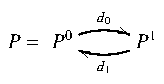
\includegraphics[width=0.30\textwidth]{figures/Fig_114_PDF210_Book198.pdf}
    \caption{分次矩阵分解（原书 p.198）}
    \label{fig:graded-matrix-factorization}
  \end{figure}
  \item 分次矩阵分解 $P$ 的同调移位为
  \[
    P[1]=P_1\underset{-d_0}{\overset{-d_1}{\rightleftarrows}}P_0(w).
  \]
  注意，$P[2]$ 与 $P(w)$ 相同，其中 $(w)$ 表示 $R$-分次的移位。
  \begin{figure}[H]\centering
    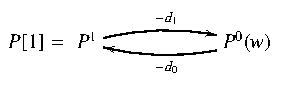
\includegraphics[width=0.34\textwidth]{figures/Fig_115_PDF210_Book198.pdf}
    \caption{矩阵分解的同调移位（原书 p.198）}
    \label{fig:graded-matrix-factorization-shift}
  \end{figure}
  \item 若 $P,Q$ 是两个分次矩阵分解，则定义
  \[
    \operatorname{Hom}^{\bullet}(P,Q)
    =\bigoplus_i\operatorname{grHom}_R(P_0,Q[i]_0)
      \oplus\operatorname{grHom}_R(P_1,Q[i]_1),
  \]
  其中 $\operatorname{grHom}_R(X,Y)$ 表示保持次数的 $R$-模态射。在这个空间上，标准微分关于同调分次的次数为 $1$。
  \item 分次矩阵分解范畴\index{fencijuzhenfenjiefanchou@分次矩阵分解范畴|hyperpage} $\mathrm{grMF}^{\bullet}(R,W)$ 是具有上述对象与态射的 dg-范畴的极小模型。
\end{itemize}
\end{definition}

\begin{example}[分次矩阵分解的不同实现]
回到 $R=\mathbb C[X,Y]$ 与 $W=XY(X-Y)$。把 $W$ 分解为 $X$ 与 $Y(X-Y)$，所得普通矩阵分解在忽略同调移位后，可以有三种不同的分次矩阵分解实现，如下图所示。
\begin{figure}[H]\centering
  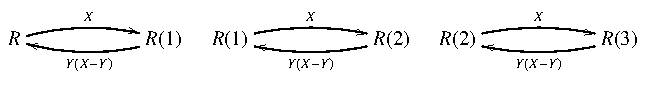
\includegraphics[width=0.92\textwidth]{figures/Fig_116_PDF211_Book199.pdf}
  \caption{例 7.70 中的三种分次矩阵分解（原书 p.199）}
  \label{fig:graded-factorization-three-gradings}
\end{figure}
\end{example}

分次矩阵分解的更多细节见 Orlov 的工作\bookcite{200}；其主要定理也将在下一节讨论。Landau--Ginzburg 模型还可以推广到非仿射\bookcite{201,225}或带栈结构\bookcite{216}的情形。此外，关于稳定表示范畴已有大量文献；它是奇点范畴的非交换类比\bookcite{46,108}。

\section{等价}\label{sec:equivalences}
\takeaway{Fano 与反 Fano 簇可由导出范畴借助 Serre 函子重构；Fourier--Mukai 核 $P\in D\mathrm{Coh}^{\bullet}(X\times Y)$ 给出函子 $\Phi_P=D\pi_{Y*}\circ(-\otimes P)\circ D\pi_X^*$，Orlov 定理说光滑射影簇间的正合函子皆源于此；模空间与倾斜把 $D\mathrm{Coh}^{\bullet}X$ 与箭图表示、$\mathrm{Perf}^{\bullet}A$ 联系起来。}
我们已经看到，$B$ 模型有许多不同形式，而不同的 $B$ 模型往往会导出等价或相关的范畴。本节将更深入地研究这一现象。

\subsection{重构簇}\label{subsec:reconstructing-varieties}
若 $A$ 是一个代数，则每个 $r\in Z(A)$ 都给出自然变换
\[
  \nu_r\colon 1_{\mathrm{Mod}A}\longrightarrow1_{\mathrm{Mod}A},
\]
它把模 $M$ 上对应于乘以 $r$ 的映射赋给 $M$。这确实是自然变换，因为 $r$ 的作用与所有模态射相容。反过来，任意从恒等函子到自身的自然变换都具有这种形式：令 $r=\nu_A(1)$。对任意模 $M$ 及元素 $m\in M$，定义模态射 $\phi_m\colon A\to M$，使 $\phi_m(1)=m$，则
\[
  \nu_M(m)=\nu_M(\phi_m(1))=\phi_m(\nu_A(1))=\phi_m(r)=rm.
\]
同样的论证也适用于包含 $A$ 本身的其他模范畴，例如 $\mathrm{Mod}A$、$D\mathrm{Mod}^{\bullet}A$ 和 $\mathrm{Perf}^{\bullet}A$。对仿射簇，这给出
\[
  \operatorname{End}(1_{D\mathrm{Coh}^{\bullet}X})
  \cong \operatorname{End}(1_{D\mathrm{Mod}^{\bullet}V(R)})\cong R.
\]
换言之，我们可以从仿射簇的导出范畴重构该簇：它就是
\[
  V\bigl(\operatorname{End}(1_{D\mathrm{Coh}^{\bullet}X})\bigr).
\]

对拟射影簇，这种方法通常行不通，因为它们的整体函数往往很少。此时，我们希望把簇写成某个分次环 $R$ 的 $\mathbb P(R)$。与仿射簇的坐标环不同，分次环 $R$ 并不能由 $X$ 唯一确定。取而代之的是，存在一个线丛 $L=\mathcal O(1)$，使
\[
  R=\bigoplus_{i\geq0}L^{\otimes i}(X).
\]

\begin{definition}{极丰富线丛与丰富线丛}{very-ample-ample-line-bundle}
若线丛 $L$ 满足 $X=\mathbb P(R_L)$，其中
\[
  R_L:=\bigoplus_{i\geq0}L^{\otimes i}(X),
\]
则称 $L$ 为极丰富线丛\index{jifengfuxiancong@极丰富线丛|hyperpage}；若存在 $k\geq1$ 使 $L^{\otimes k}$ 极丰富，则称 $L$ 为丰富线丛\index{fengfuxiancong@丰富线丛|hyperpage}。
\end{definition}

\begin{example}[射影直线上的丰富线丛]
一般而言，一个射影簇可以有许多丰富线丛。对 $\mathbb P^1$，所有 $\mathcal O(i)$（$i>0$）都是丰富的。以 $L=\mathcal O(2)$ 为例，则
\[
  R_L=\bigoplus_{i\geq0}\mathcal O(2i)(\mathbb P^1)
  =\mathbb C[X^2,Y^2,XY]
  \cong\frac{\mathbb C[U,V,W]}{(UV-W^2)}.
\]
由后一种描述可知，$\mathbb P(R_L)$ 可看作 $\mathbb P^2$ 中的圆锥曲线 $UV-W^2=0$。它通过 Veronese 嵌入
\[
  (x:y)\longmapsto(x^2:y^2:xy)
\]
与 $\mathbb P^1$ 同构。
\end{example}

从范畴角度看，我们可以把 $R_L$ 重构为自然变换空间。任一线丛都定义了 $\mathrm{Vect}(X)$ 上的自函子 $-\otimes L$：
\[
  (M\otimes L)(U):=M(U)\otimes_{\mathcal O(U)}L(U).
\]
这个函子在 $\mathrm{Vect}^{\bullet}(X)$ 上诱导 dg-函子，并在其导出范畴 $D\mathrm{Vect}^{\bullet}X=\mathrm{Perf}^{\bullet}X$ 上诱导一个 $A_\infty$ 函子 $T$（在导出范畴语境中，通常把它记为 $-\otimes^{\mathbf L}L$）。$L$ 的整体截面对应于恒等函子到 $T$ 的自然变换：
\[
  L(X)=\operatorname{Fun}(1,T).
\]
这里 $\operatorname{Fun}$ 表示从 $\mathrm{Perf}^{\bullet}X$ 到自身的函子范畴，其态射为自然变换。因为 $T$ 可逆，且 $T^{-1}=-\otimes L^{-1}$、$L^{-1}=\operatorname{Hom}(L,\mathcal O_X)$，故
\[
  \operatorname{Fun}(T^i,T^j)
  =\operatorname{Fun}(1,T^{j-i})
  =\operatorname{Fun}(1,-\otimes L^{j-i}).
\]
因此
\[
  R_T:=\bigoplus_{i\geq0}\operatorname{Fun}(1,T^i)
\]
通过复合获得环结构，并且与 $R_L$ 同构。于是，重构簇的问题归结为找到合适的 $T$。

如定义~\ref{def:tangent-cotangent-canonical-sheaves} 所述，簇上有一个内蕴地定义的线丛，即典范线丛。但是，它未必丰富，因此未必适合上述方法。为此，我们区分以下几类簇。

\begin{definition}{Fano 簇、Calabi--Yau 簇与反 Fano 簇}{fano-calabi-yau-antifano}
光滑射影簇 $X$ 称为：
\begin{itemize}
  \item 若反典范线丛 $K^{-1}$ 丰富，则称为 Fano 簇\index{fanocu@Fano 簇|hyperpage}；
  \item 若典范线丛平凡，即 $K=\mathcal O_X$，则称为 Calabi--Yau 簇\index{calabiyaucu@Calabi–Yau 簇|hyperpage}；
  \item 若典范线丛 $K$ 丰富，则称为反 Fano 簇\index{fanfanocu@反 Fano 簇|hyperpage}。
\end{itemize}
\end{definition}

\begin{note}\label{note:three-variety-types-curvature}
\textbf{注 7.74.} 这三种情形并未穷尽所有可能，但它们代表了三个基本类型，大致分别对应正曲率、零曲率和负曲率的流形。
\end{note}

\begin{example}[射影空间超曲面的分类]
射影空间 $\mathbb P^n$ 是 Fano 簇，因为 $K^{-1}=\mathcal O(n+1)$ 丰富。设 $f$ 是环 $R=\mathbb C[X_0,\ldots,X_n]$ 中次数为 $k$ 的齐次函数。由伴随公式\bookcite{109}，若 $\mathbb P(R/(f))$ 光滑，则当 $k<n+1$ 时它是 Fano 簇；当 $k=n+1$ 时它是 Calabi--Yau 簇；当 $k>n+1$ 时它是反 Fano 簇。

取 $n=2$，这也说明了前述曲率类比：当 $k=1,2$ 时，$\mathbb P(R/(f))$ 是 Fano 簇，即射影直线或二次曲线，因而同构于黎曼球面。当 $k=3$ 时所得簇是 Calabi--Yau 簇，即椭圆曲线；它是环面，故为平坦的。反 Fano 情形对应于亏格更高、具有负曲率的曲线。
\end{example}

这些讨论表明，如果光滑射影簇是 Fano 簇或一般型簇，我们或许可以从其导出范畴 $D\mathrm{Coh}^{\bullet}X=\mathrm{Perf}^{\bullet}X$ 重构它，因为此时可以尝试寻找函子 $-\otimes K$。

\begin{theorem}{Bondal--Orlov 重构定理}{bondal-orlov-reconstruction}
若 $X$ 是 Fano 簇或反 Fano 簇，则可以从 $D\mathrm{Coh}^{\bullet}X$ 重构 $X$。
\end{theorem}
\begin{proof}[证明思路]
证明的主要工具是 Serre 函子\index{serrehanzi@Serre 函子|hyperpage}。若 $\mathcal C$ 是 $k$-线性范畴，若存在函子 $F\colon\mathcal C\to\mathcal C$ 及自然同构
\[
  \nu_{X,Y}\colon\mathcal C(X,Y)\longrightarrow\mathcal C(Y,F(X))^\vee,
\]
其中 $(-)^\vee$ 表示 $k$-线性对偶，则称 $F$ 为 Serre 函子。若范畴有 Serre 函子，它在自然同构意义下唯一，因此是范畴的内在对象。$n$ 维光滑射影簇 $X$ 的导出范畴有 Serre 函子 $-\otimes K[n]$。当 $K$ 或 $K^{-1}$ 丰富时，Bondal 与 Orlov\bookcite{32}利用该 Serre 函子在导出范畴中识别点层\index{dianceng@点层|hyperpage}与线丛。
\end{proof}
% [Tutor Note: 原书把 Serre 函子的自然同构印作 $\nu_{X,Y}\colon\mathcal C(X,Y)\to\mathcal C(F(Y),X)^\vee$，这与紧接着所说的“$n$ 维光滑射影簇的导出范畴有 Serre 函子 $-\otimes K[n]$”不相容（按该书面公式，$-\otimes K[n]$ 满足的是关于 $F^{-1}$ 的关系）。译文采用标准方向 $\mathcal C(X,Y)\cong\mathcal C(Y,F(X))^\vee$；核对 Serre 对偶时可写成 $\operatorname{Hom}(X,Y)\cong\operatorname{Hom}(Y,X\otimes K[n])^\vee$，方向记反是最常见的错误。]

\subsection{Fourier--Mukai 变换}\label{subsec:fourier-mukai-transforms}
若簇不是 Fano 簇或一般型簇，则可能出现非同构簇却具有等价导出范畴的情形。为寻找这类现象的例子，我们先介绍一大类定义在相干层导出范畴之间的函子，再考察它们何时是等价。

这一构造的灵感来自 Fourier 分析。若 $f\colon\mathbb R\to\mathbb C$ 是函数，可以定义其 Fourier 变换
\[
  \mathcal F(f)\colon\mathbb R\to\mathbb C,
  \qquad y\longmapsto\int_{\mathbb R}f(x)e^{-ixy}\,dx.
\]
虽然这个运算把 $\mathbb R$ 上的函数变为 $\mathbb R$ 上的函数，但更好的看法是：它把一个空间 $X=\mathbb R$（位置空间）上的函数变成另一个空间 $Y$（动量空间）上的函数，只不过此处 $Y$ 恰好也同构于 $\mathbb R$。若把 $X$ 换成圆周 $S^1$，这一点就更明显：此时 $Y=\mathbb Z$，Fourier 变换把周期函数变成它的 Fourier 级数。

Fourier 变换具体如何作用？它先沿投影 $\pi_X\colon X\times Y\to X$ 把 $X$ 上的函数拉回到 $X\times Y$，再乘以 $X\times Y$ 上的一个函数，最后对 $X$ 分量积分消去。下面我们试着把这个过程从函数推广到层。

\begin{definition}{簇的笛卡尔积}{product-of-varieties}
若 $X,Y$ 是仿射簇，定义它们的笛卡尔积\index{dikaerji@笛卡尔积|hyperpage}为
\[
  X\times Y:=V(\mathcal O_X\otimes_{\mathbb C}\mathcal O_Y).
\]
若 $X,Y$ 是簇，分别有开覆盖 $\mathcal U=\{U_i:i\in I\}$ 和 $\mathcal V=\{V_j:j\in J\}$，则定义 $X\times Y$ 为由 $U_i\times V_j$ 覆盖、并配备显然粘合映射的簇。
\end{definition}

\begin{note}\label{note:product-topology-varieties}
\textbf{注 7.78.} 作为集合，$X\times Y$ 确实是 $X$ 与 $Y$ 的乘积；但就 Zariski 拓扑而言，它一般不是两个拓扑空间的乘积。此外可以证明，若 $X,Y$ 都光滑，则 $X\times Y$ 也光滑。
\end{note}

现在设 $X,Y$ 是光滑簇，且 $P^{\bullet}$ 是 $\mathrm{Perf}^{\bullet}(X\times Y)$ 中的对象。我们分三步构造一个函子。
\begin{enumerate}[label=(\roman*)]
  \item \textbf{提升到乘积空间。} 若 $M$ 是 $X$ 上的层，定义
  \[
    (\pi_X^*M)(U_i\times V_j):=M(U_i)\otimes_{\mathbb C}\mathcal O(V_j).
  \]
  若 $M$ 局部自由，则 $\pi_X^*M$ 也局部自由。因此这给出函子 $\pi_X^*\colon\mathrm{Vect}(X)\to\mathrm{Vect}(X\times Y)$，并进而给出 $A_\infty$ 函子
  \[
    D\pi_X^*\colon\mathrm{Perf}^{\bullet}(X)\to\mathrm{Perf}^{\bullet}(X\times Y).
  \]
  \item \textbf{与 $P^{\bullet}$ 张量。} 对簇 $V$ 上有限生成的局部自由层复形 $P^{\bullet}$（此处 $V=X\times Y$），可以定义层函子
  \[
    -\otimes P^{\bullet}\colon\mathrm{Vect}^{\bullet}V\longrightarrow\mathrm{Vect}^{\bullet}V,
    \qquad M^{\bullet}\longmapsto(M\otimes P)^{\bullet},
  \]
  其中
  \[
    (M\otimes P)^i(U)=\bigoplus_{k+\ell=i}M^k(U)\otimes P^{\ell}(U),
    \qquad d_{M\otimes P}=d_M\otimes1_P\pm1_M\otimes d_P.
  \]
  取 Čech 上同调后便得到 $A_\infty$ 函子
  \[
    D(-\otimes P)\colon\mathrm{Perf}^{\bullet}V\to\mathrm{Perf}^{\bullet}V.
  \]
  \item \textbf{对 $X$ 积分消去。} 若 $N$ 是 $X\times Y$ 上的层，我们希望令
  \[
    (\pi_{Y*}N)(V_j)=N(X\times V_j).
  \]
  但从 $A_\infty$ 的角度看，这个运算并不理想。事实上，$N(X\times V_j)$ 是层 $N(-\times V_j)\colon U_i\mapsto N(U_i\times V_j)$ 的零次 Čech 上同调；这种做法取了一个复形的同调，性质并不好。更好的办法是保留整个复形：
  \[
    (D\pi_{Y*}N)(V_j)=\check C\bigl(N(-\times V_j);\mathcal U\bigr).
  \]
  这样会把局部自由层变为局部自由层的复形。不过，这类复形未必有限生成，故得到的函子是
  \[
    D\pi_{Y*}\colon\mathrm{Perf}^{\bullet}(X\times Y)\to D\mathrm{VECT}^{\bullet}Y.
  \]
\end{enumerate}

\begin{note}\label{note:pushforward-perfect}
\textbf{注 7.79.} 一般而言，$N(U_i\times V_j)$ 不是有限生成的 $\mathcal O(V_j)$-模，所以这些 Čech 复形属于 $D\mathrm{VECT}^{\bullet}Y$，而非 $\mathrm{Perf}^{\bullet}Y$。不过，若 $X$ 是光滑射影簇，这些复形的上同调有限秩，因此 $D\pi_{Y*}$ 可以视为取值于 $\mathrm{Perf}^{\bullet}(Y)$ 的函子。
\end{note}

\begin{definition}{Fourier--Mukai 核与变换}{fourier-mukai-transform}
设 $X,Y$ 是光滑射影簇。Fourier--Mukai 核是对象 $F\in D\mathrm{Coh}^{\bullet}(X\times Y)$。把 $F$ 表示为 $X\times Y$ 上局部自由层组成的复形 $P^{\bullet}\in\mathrm{Vect}^{\bullet}(X\times Y)$，则相应的 Fourier--Mukai 变换\index{fouriermukaibianhuan@Fourier–Mukai 变换|hyperpage}是函子
\[
  \mathcal F_F:=D\pi_{Y*}\circ D(-\otimes P^{\bullet})\circ D\pi_X^*
  \colon\mathrm{Perf}^{\bullet}X\longrightarrow\mathrm{Perf}^{\bullet}Y.
\]
\end{definition}
% [Tutor Note: 合成顺序不可交换：$\Phi_P=D\pi_{Y*}\circ D(-\otimes P)\circ D\pi_X^*$ 是先沿 $\pi_X$ 拉回到 $X\times Y$、与核 $P$ 张量、再沿 $\pi_Y$ 推前，得到 $\mathrm{Perf}^{\bullet}X\to\mathrm{Perf}^{\bullet}Y$。核所在空间与函子方向的对应是：$P\in D\mathrm{Coh}^{\bullet}(X\times Y)$ 决定 $X\to Y$，把 $P$ 换成它在交换因子后的转置才给出反向函子；$p_2^*\mathcal E\otimes p_1^*(-)$ 的写法只是把拉回与张量换序的等价格式，不能据此调换 $X,Y$。]

\begin{example}[几种熟悉的函子]
Fourier--Mukai 变换的适用范围很广，能够描述一些熟知的函子。
\begin{itemize}
  \item 若 $Y$ 是一点，可以把结构层 $\mathcal O_X$ 看成 $X\times Y$ 上的层。对应的 Fourier--Mukai 变换把 $X$ 上的层 $S$ 送到它的 Čech 上同调，并将其视为 $\mathrm{Perf}^{\bullet}Y=\mathrm{vect}^{\bullet}_{\mathbb C}$ 中的对象。
  \item 令 $X=Y$，并考虑对角线的结构层
  \[
    \mathcal O_{\Delta}(U_i\times U_j)=\mathcal O_X(U_i\cap U_j).
  \]
  以 $\mathcal O_\Delta$ 为核的 Fourier--Mukai 变换同构于恒等函子。这类似于公式
  \[
    \int_{\mathbb R}f(y)\delta(x-y)\,dy=f(x),
  \]
  其中 $\delta$ 是 Dirac δ 函数。
  \item 若 $S$ 是 $X$ 上的可逆层，可以把它变成一个集中在对角线上的 $X\times X$ 上的层：
  \[
    S_\Delta(U_i\times U_j)=S_X(U_i\cap U_j).
  \]
  以 $S_\Delta$ 为核的 Fourier--Mukai 变换对应于与 $S$ 张量。
  \item 若 $\phi\colon X\to Y$ 是簇态射，则可构造其图像的结构层
  \[
    \mathcal O_\Gamma(U)=\frac{\mathcal O_{X\times Y}(U)}{(f\mid f(x,\phi(x))=0)}.
  \]
   以 $\mathcal O_\Gamma$ 为核的 Fourier--Mukai 变换对应于沿 $\phi$ 的导出推前。
\end{itemize}
在以上例子中，点层都被送到点层。不过，还有更精细的例子。
\end{example}

\begin{example}[椭圆曲线上的 Fourier--Mukai 等价]
考虑椭圆曲线 $E=\mathbb P(R)$，其中
\[
  R=\mathbb C[X,Y,Z]/(Y^2Z-X^3+XZ^2).
\]
对每个点 $P\in E$，都有一个线丛 $L_P=\mathcal O(P-P_\infty)$（参见例~\ref{ex:divisor-sheaf}）。为了区分椭圆曲线的两个副本——一个参数化点，另一个参数化线丛——把后者记作 $E^\vee$。

我们可以把这些线丛汇集为 $E^\vee\times E$ 上的一个大线丛 $T$，其在 $(P,Q)$ 处的纤维就是 $L_P$ 在 $Q$ 处的纤维。这个线丛称为 Poincaré 线丛。以它为核，可以定义从 $D\mathrm{Coh}^{\bullet}E^\vee$ 到 $D\mathrm{Coh}^{\bullet}E$ 的 Fourier--Mukai 变换；该变换把 $P$ 处的点层送到线丛 $L_P$。可以证明，这个函子实际上是一个等价。

Mukai\bookcite{183}把这一构造推广到高维，得到阿贝尔簇 $A$ 与其对偶簇 $A^\vee$ 之间的等价。这由此给出了不同簇之间导出等价的第一个例子。
\end{example}

本节最后介绍 Orlov 的一个漂亮定理：若限制在光滑射影簇上，Fourier--Mukai 构造足以描述簇之间所有相关的导出等价。

\begin{theorem}{Orlov 定理\bookcite{198}}{orlov-fourier-mukai}
光滑射影簇的导出范畴之间的每个正合函子，都同构于某个 Fourier--Mukai 变换。
\end{theorem}

Fourier--Mukai 变换的更多内容可参阅 Huybrechts 的专著\bookcite{124}。

\subsection{模空间}\label{subsec:moduli-spaces}
上一个例子中，我们使用了参数化 $D\mathrm{Coh}^{\bullet}E$ 中某些对象（次数为零的线丛）的空间 $E^\vee$。这个空间使我们能够把 $D\mathrm{Coh}^{\bullet}E$ 中的对象变换为 $D\mathrm{Coh}^{\bullet}E^\vee$ 中的对象。当然，这个想法并不局限于相干层的导出范畴，也可以用于其他范畴。

设 $A=\mathbb C Q/I$ 是带关系的箭图路径代数，并固定维数向量 $\alpha\colon Q_0\to\mathbb N$。定义表示空间
\[
  \operatorname{Rep}(Q,\alpha)
  :=\bigoplus_{a\in Q_1}\operatorname{Mat}_{\alpha_{h(a)}\times\alpha_{t(a)}}(\mathbb C),
\]
它可视为一个大仿射空间，其坐标环为
\[
  R=\mathbb C[X^a_{ij}\mid a\in Q_1,
       1\leq i\leq\alpha_{h(a)},\ 1\leq j\leq\alpha_{t(a)}].
\]
此空间中的每个点由一个 $|Q_1|$ 元组的矩阵 $(\rho_a)_{a\in Q_1}$ 表示，并对应一个表示 $\rho\colon\mathbb C Q\to\operatorname{Mat}_{n\times n}(\mathbb C)$，其中 $n=\sum_{v\in Q_0}\alpha_v$；对每条箭头 $a$，该表示把 $\rho_a$ 放入相应的分块矩阵中。我们可以把这些表示汇集成 $\operatorname{Rep}(Q,\alpha)$ 上的向量丛 $\operatorname{Rep}(Q,\alpha)\times\mathbb C^n$。在代数一侧，这对应于自由 $R$-模 $T=R\otimes\mathbb C^n$ 及模态射 $\rho\colon\mathbb C Q\to\operatorname{End}_R(T)$。

表示空间中的许多点对应同构的表示。为处理这一点，考虑换基群
\[
  \mathrm{GL}_\alpha:=\prod_{v\in Q_0}\mathrm{GL}_{\alpha_v}(\mathbb C),
\]
它在 $\operatorname{Rep}(Q,\alpha)$ 上的作用为
\[
  (g\cdot\rho)_a=g_{h(a)}\rho_a g^{-1}_{t(a)}.
\]
该作用的轨道恰好是表示的同构类。一个自然想法是取这个群作用的商\index{gitshang@GIT 商|hyperpage}，即考虑不变量环所对应的簇：
\[
  \operatorname{Rep}(Q,\alpha)//\mathrm{GL}_\alpha
  :=V(R^{\mathrm{GL}_\alpha}).
\]
与有限群的情形不同，这个商并不能参数化全部轨道。若群是无限的，一个轨道可能包含在另一个轨道的闭包中；此时每个不变量函数在这两个轨道上都取相同值，因此它们在商空间中对应同一点。

\begin{example}[Kronecker 箭图的商]
令 $Q$ 为下图所示的 Kronecker 箭图，并令 $\alpha=(1,1)$。于是 $\operatorname{Rep}(Q,\alpha)=\mathbb C^2$，$\mathrm{GL}_\alpha=(\mathbb C^*)^2$，且
\begin{figure}[H]\centering
  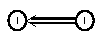
\includegraphics[width=0.20\textwidth]{figures/Fig_117_PDF218_Book206.pdf}
  \caption{例 7.84 中的箭图（原书 p.206）}
  \label{fig:kronecker-quiver-example-784}
\end{figure}
\[
  (g,h)\cdot(x,y)=(gxh^{-1},gyh^{-1}).
\]
该作用的轨道是去掉原点的直线 $\mathbb C(x,y)\setminus\{(0,0)\}$ 与零轨道 $\{(0,0)\}$；零轨道包含在所有其他轨道的闭包中。因此，范畴商只有一个点。事实上，坐标环为 $R=\mathbb C[X,Y]$，作用为
\[
  (g,h)\cdot X=gXh^{-1},\qquad(g,h)\cdot Y=gYh^{-1},
\]
所以 $R^{\mathrm{GL}_\alpha}=\mathbb C$，且 $\operatorname{Rep}(Q,\alpha)//\mathrm{GL}_\alpha=\{p\}$。

我们可以先丢弃不好的轨道，再取商。这样得到
\[
  \mathbb C^2\setminus\{(0,0)\}/\mathrm{GL}_\alpha=\mathbb P^1,
\]
这是一个射影簇，它分类除零表示外的所有轨道。这个商可以写作 $\mathbb P(R)$，其中 $R$ 按群作用分次：若 $f\in R$ 满足
\[
  (g,h)\cdot f=g^nh^{-n}f,
\]
就称 $f$ 的次数为 $n$。
\end{example}

上述例子可以推广为几何不变量理论（GIT）商。\footnote{GIT 是 geometric invariant theory（几何不变量理论）的缩写。}对每个向量 $\theta\colon Q_0\to\mathbb Z$，可构造乘法特征
\[
  \chi_\theta\colon\mathrm{GL}_\alpha\to\mathbb C^*,
  \qquad g\longmapsto\prod_{v\in Q_0}\det(g_v)^{\theta_v}.
\]
若 $f\in R$ 满足 $g\cdot f=\chi_\theta(g)f$，则称 $f$ 为 $\theta$-半不变量\index{banbubianliang@半不变量|hyperpage}。半不变量环\index{banbubianlianghuan@半不变量环|hyperpage}是各次幂 $\chi_\theta^n$ 对应半不变量空间的直和：
\[
  R_\theta:=\bigoplus_{n=0}^{\infty}
  \{f\in R\mid\text{对所有 }g\in\mathrm{GL}_\alpha,
  \ g\cdot f=\chi_\theta(g)^nf\}.
\]
这是一个分次环，其零次部分为不变量环 $R^{\mathrm{GL}_\alpha}$。簇 $\mathbb P(R_\theta)$ 可由开集
\[
  U_f=V\bigl((R_\theta[f^{-1}])_0\bigr),\qquad f\in(R_\theta)_n,
\]
覆盖。环 $R_\theta[f^{-1}]_0$ 的元素可看作定义在
$\{\rho\in\operatorname{Rep}(Q,\alpha)\mid f(\rho)\ne0\}$ 上的不变量函数，因此
\[
  U_f=\{\rho\in\operatorname{Rep}(Q,\alpha)\mid f(\rho)\ne0\}//\mathrm{GL}_\alpha.
\]

\begin{definition}{$\theta$-半稳定表示及其模空间}{theta-semistable-moduli}
若存在 $f\in(R_\theta)_{>0}$ 使 $f(\rho)\ne0$，则称表示 $\rho$ 为 $\theta$-半稳定表示\index{banwendingbiaoshi@半稳定表示|hyperpage}\index{wendingbiaoshi@稳定表示|hyperpage}。$\theta$-半稳定表示的模空间定义为
\[
  M_\theta(Q,\alpha):=\mathbb P(R_\theta),
\]
也可解释为
\[
  \operatorname{Rep}^{\theta\text{-ss}}(Q,\alpha)//\mathrm{GL}_\alpha
  :=\{\rho\in\operatorname{Rep}(Q,\alpha)\mid\rho\text{ 为 }\theta\text{-半稳定表示}\}//\mathrm{GL}_\alpha.
\]
\end{definition}

一般而言，两个不同构的 $\theta$-半稳定表示仍可能对应 $M_\theta(Q,\alpha)$ 中的同一点。这会在轨道大小不同时发生，因为较小的轨道可能包含在较大轨道的闭包中。最大的轨道对应于稳定子尽可能小的表示；最小稳定子就是标量矩阵群 $\mathbb C^*\subset\mathrm{GL}_\alpha$。因此，若一个半稳定表示的稳定子恰为 $\mathbb C^*$，就称它为 $\theta$-稳定表示。

(半)稳定性的定义来自 $\mathrm{GL}_\alpha$ 在簇 $\operatorname{Rep}(Q,\alpha)$ 上的群作用，但它也有一个漂亮的箭图表示论解释。

\begin{theorem}{King 稳定性判据}{king-stability-criterion}
表示 $\rho\in\operatorname{Rep}(Q,\alpha)$ 是 $\theta$-稳定的（$\theta$-半稳定的），当且仅当 $\theta\cdot\alpha=0$，且对每个真子表示，其维数向量 $\beta$ 都满足 $\theta\cdot\beta>0$（$\theta\cdot\beta\geq0$）。
\end{theorem}
\begin{proof}[证明思路]
这里只说明这种联系的主要思路，完整细节参见\bookcite{138}。首先，非零 $n\theta$-半不变量的存在蕴含 $\theta\cdot\alpha=0$，因为标量矩阵 $\lambda 1$ 对 $\rho$ 的作用平凡：
\[
  f(\rho)=f(\lambda1\cdot\rho)=\chi_\theta(\lambda1)^n f(\rho)
  =\lambda^{n\theta\cdot\alpha}f(\rho).
\]
若表示 $\rho$ 有维数向量为 $\beta$ 的子表示，就可将它写成分块上三角形式。用
\[
  g_t=\begin{pmatrix}t1_\beta&0\\0&1_{\alpha-\beta}\end{pmatrix}
\]
作共轭。由于表示具有上述分块上三角形式，极限 $\lim_{t\to0}g_t\cdot\rho$ 存在。但若 $f$ 是 $n\theta$-半不变量，则
\[
  f(g_t\cdot\rho)=t^{n\theta\cdot\beta}f(\rho).
\]
若 $\theta\cdot\beta<0$，当 $t\to0$ 时右侧没有极限，这就产生矛盾。
\end{proof}

\begin{definition}{泛型稳定条件}{generic-stability-condition}
若 $\theta\cdot\alpha=0$ 且对每个非零维数向量 $\beta<\alpha$ 都有 $\theta\cdot\beta\ne0$，则称稳定条件\index{fanxingwendingtiaojian@泛型稳定条件|hyperpage} $\theta$ 关于 $\alpha$ 是泛型的。这意味着 $\theta$-半稳定与 $\theta$-稳定两种概念一致。
\end{definition}

\begin{theorem}{King 模空间光滑性定理\bookcite{138}}{king-moduli-smoothness}
若 $\theta$ 是泛型的，则 $M_\theta(Q,\alpha)$ 是光滑簇，其点对应于 $Q$ 的 $\theta$-稳定 $\alpha$ 维表示的同构类。
\end{theorem}
\begin{proof}[证明思路]
空间 $\operatorname{Rep}^{\theta\text{-ss}}(Q,\alpha)$ 是光滑空间 $\operatorname{Rep}(Q,\alpha)$ 的开子集，故自身光滑。投影
\[
  \pi\colon\operatorname{Rep}^{\theta\text{-ss}}(Q,\alpha)
  \longrightarrow M_\theta(Q,\alpha)
\]
的纤维都同构于光滑簇 $\mathrm{GL}_\alpha/\mathbb C^*$，因而目标空间也必为光滑簇。
\end{proof}

\begin{example}[Kronecker 箭图表示的稳定模空间]
回到维数向量为 $\alpha=(1,1)$ 的 Kronecker 箭图。根据 $\theta=(\theta_1,\theta_2)$ 的不同取值，情况如下：
\begin{itemize}
  \item 若 $\theta_1+\theta_2\ne0$，则不存在 $\theta$-半不变量，故 $R_\theta=\mathbb C$、$\mathbb P(R_\theta)=\varnothing$。由于 $\alpha\cdot\theta\ne0$，不存在 $\theta$-半稳定表示，所以 $M_\theta(Q,\alpha)=\varnothing$。
  \item 若 $\theta_1=-\theta_2=0$，常数函数是 $\theta$-半不变量，故 $R_\theta=\mathbb C\oplus\mathbb C\oplus\cdots$，且 $\mathbb P(R_\theta)=\{p\}$。注意，此时 $\theta$ 不是泛型条件。所有表示都半稳定，但没有稳定表示。每个轨道的闭包都包含零轨道，因此 $M_\theta(Q,\alpha)$ 只有一个点。
  \item 若 $\theta_1=-\theta_2=k>0$，次数为 $k$ 的函数是 $\theta$-半不变量，故
  $R_\theta=\mathbb C\oplus R_k\oplus R_{2k}\oplus\cdots$，并且 $\mathbb P(R_\theta)=\mathbb P^1$。此时除零轨道外，所有表示都稳定；零轨道有维数向量 $(0,1)$ 的子表示。
  \item 若 $\theta_1=-\theta_2=k<0$，不存在 $\theta$-半不变量，故 $R_\theta=\mathbb C$ 且 $\mathbb P(R_\theta)=\varnothing$。此时没有稳定表示，因为每个表示都有维数向量 $(1,0)$ 的子表示。
\end{itemize}

若 $\theta$ 泛型，我们便能按同构分类所有 $\theta$-稳定表示。每个这样的表示都可视为一个带有 $\mathbb C Q$ 作用的向量空间 $\mathbb C^n$。自然的问题是：能否把这些表示组成 $M_\theta(Q,\alpha)$ 上的向量丛？朴素做法是考虑丛 $\operatorname{Rep}(Q,\alpha)\times\mathbb C^n\to\operatorname{Rep}(Q,\alpha)$，限制到稳定表示子空间后再对 $\mathrm{GL}_\alpha$ 取商。不幸的是，这样做行不通，因为每个点 $(\rho,x)$ 的轨道中都有 $(\rho,\lambda x)$（回忆标量 $\lambda\in\mathrm{GL}_\alpha$ 对 $\rho$ 的作用平凡）。于是 $(\rho,0)$ 落在所有 $(\rho,x)$ 的轨道闭包中，商仍只是 $M_\theta(Q,\alpha)$。

为避免这种情况，假设存在群态射 $\sigma\colon\mathrm{GL}_\alpha\to\mathbb C^*$，使其在 $\mathbb C^*\subset\mathrm{GL}_\alpha$ 上满足 $\sigma(\lambda)=\lambda$。把 $\mathrm{GL}_\alpha$ 在向量丛上的作用改为
\[
  g(\rho,x):=(g\cdot\rho,\sigma(g)^{-1}gx).
\]
这样标量在 $x$ 上的作用变为平凡，因而可对 $\operatorname{Rep}^{\theta\text{-ss}}(Q,\alpha)\times\mathbb C^n$ 取这个新作用的商。所得商称为泛丛；它可以视为 $M_\theta(Q,\alpha)$ 上的 $\mathbb C Q$-模层。
\end{example}

与交换情形类似，Fourier--Mukai 核可视为 $X$ 上的、以 $Y$ 上层为纤维的层；泛丛则是 $M_\theta(Q,\alpha)$ 上的、以与非交换代数 $\mathbb C Q$ 对应的非交换簇上的层为纤维的层。由此可定义非交换 Fourier--Mukai 变换
\[
  F\colon D\mathrm{Coh}^{\bullet}M_\theta(Q,\alpha)
  \longrightarrow D\mathrm{Mod}^{\bullet}\mathbb C Q.
\]

\begin{example}[Kronecker 模空间上的泛丛]
回到 $\alpha=(1,1)$、$\theta=(1,-1)$ 的 Kronecker 箭图，取 $\sigma(g,h)=h$。在
\[
  T=\mathbb C[X,Y]\otimes\mathbb C^2
  =\mathbb C[X,Y]e_1\oplus\mathbb C[X,Y]e_2
\]
上，$\mathrm{GL}_\alpha$ 的作用为
\[
  (g,h)e_1=h^{-1}ge_1,\qquad
  (g,h)e_2=h^{-1}he_2=e_2.
\]
因此，在 $M_\theta(Q,\alpha)=\mathbb P^1$ 上的重言丛为 $\mathcal O(1)\oplus\mathcal O$。

要计算 $\mathcal O(k)\in\mathrm{Perf}^{\bullet}\mathbb P^1$ 在 Fourier--Mukai 变换下的像，将它与 $T_\theta$ 张量，得到 $\mathcal O(k+1)\oplus\mathcal O(k)$。这个丛的 Čech 复形是一个无限维的分次 $\mathbb C Q$-表示。其底层两项复形为
\[
  \mathbb C[X]\oplus\mathbb C[X^{-1}]
  \xrightarrow{\ (1\quad X^k)\ }
  \mathbb C[X,X^{-1}],
  \qquad
  \mathbb C[X]\oplus\mathbb C[X^{-1}]
  \xrightarrow{\ (1\quad X^{k+1})\ }
  \mathbb C[X,X^{-1}],
\]
分别对应两项线丛的局部截面空间；图中竖直箭头给出 Kronecker 箭头在这些空间上的作用。\begin{figure}[H]\centering
  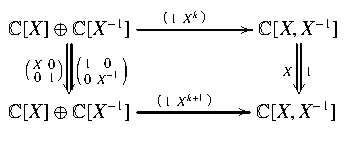
\includegraphics[width=0.90\textwidth]{figures/Fig_118_PDF221_Book209.pdf}
  \caption{例 7.90 中的 Čech 复形及箭图作用（原书 p.209）}
  \label{fig:cech-complex-tautological-bundle}
\end{figure}
水平映射是 Čech 复形的微分，竖直映射表示箭图箭头的作用。对该复形取上同调：若 $k\geq-1$，上同调集中在次数 $0$，得到表示
\[
  \mathbb C^{k+2}\xleftarrow{\left(\begin{smallmatrix}1_k\\)}\mathbb C^{k+1},
  \qquad
  \mathbb C^{k+2}\xleftarrow{\left(\begin{smallmatrix}0\\)}\mathbb C^{k+1}.
\]
若 $k<-1$，上同调集中在次数 $1$，得到表示
\[
  \mathbb C^{-k-1}\xleftarrow{\left(\begin{smallmatrix}1_k&0\end{smallmatrix}\right)}\mathbb C^{-k},
  \qquad
  \mathbb C^{-k-1}\xleftarrow{\left(\begin{smallmatrix}0&1_k\end{smallmatrix}\right)}\mathbb C^{-k}.
\]
\end{example}

\begin{note}\label{note:quiver-relations-moduli}
\textbf{注 7.91.} 模空间的构造也适用于带关系路径代数 $A=\mathbb C Q/I$。此时需要考虑子簇
\[
  \operatorname{Rep}(A,\alpha)
  =\{\rho\in\operatorname{Rep}(Q,\alpha)\mid\rho(I)=0\},
\]
或其某个不可约分支。该分支的坐标环 $R_A$ 是 $R$ 对一个 $\mathrm{GL}_\alpha$-不变理想 $i$ 取商所得。若此分支光滑且 $\theta$ 泛型，则
\[
  M_\theta(Q,\alpha)=\mathbb P\bigl(R_\theta/(i\cap R_\theta)\bigr)
\]
是光滑簇，并带有一个局部自由层，其纤维是 $\theta$-稳定的 $A$-模。由此可以构造 Fourier--Mukai 函子，但要判定该函子何时为等价并不容易。
\end{note}

\subsection{倾斜}\label{subsec:tilting}
非交换 Fourier--Mukai 变换与构造等价的另一种方法——倾斜——密切相关。

\begin{definition}{倾斜对象}{tilting-object}
设 $\mathcal C^{\bullet}$ 是一个极小且分裂闭的 $A_\infty$ 范畴。若对象 $T$ 是分裂生成元，且 $\mathcal C^{\bullet}(T,T)$ 集中在次数 $0$，则称 $T$ 为倾斜对象\index{qingxieduixiang@倾斜对象|hyperpage}。
\end{definition}

若 $T$ 是倾斜对象，则 $A=\mathcal C^{\bullet}(T,T)$ 是普通代数，因为次数原因，所有高阶乘积都为零。此外，
\[
  \mathcal C^{\bullet}\cong_\infty D^{\pi}A^{\bullet}
  \cong_\infty\mathrm{Perf}^{\bullet}A,
\]
所以所有对象都同构于有限生成投射 $A$-模所组成的有限复形。

若 $\mathcal C^{\bullet}$ 是 dg-范畴 $\mathrm{dg}\mathcal C^{\bullet}$ 的极小模型，且 $A=\mathrm{dg}\mathcal C^{\bullet}(T,T)$，则可以显式构造这些复形。对 $\mathrm{dg}\mathcal C^{\bullet}$ 中任意 $M$，复形 $\mathcal C^{\bullet}(M,T)$ 具有右 $A$-模结构，并且
\[
  d(ma)=(dm)a\pm m(da)=(dm)a,
\]
所以它实际上是右 $A$-模复形。映射
\[
  \operatorname{Hom}(-,T)\colon\mathrm{dg}\mathcal C^{\bullet}
  \longrightarrow\mathrm{TwMOD}^{\bullet}A,
  \qquad M\longmapsto\mathrm{dg}\mathcal C^{\bullet}(M,T)
\]
是一个 dg-函子。转到极小模型后，它给出 $A_\infty$ 函子
\[
  D\operatorname{Hom}(-,T)\colon\mathcal C^{\bullet}
  \longrightarrow D\mathrm{MOD}^{\bullet}A.
\]
由于 $T$ 的像是 $A$ 作为自身右模，且 $T$ 是分裂生成元，函子 $D\pi\operatorname{Hom}(-,T)$ 会把 $\mathcal C^{\bullet}$ 嵌入 $D\mathrm{MOD}^{\bullet}A$，其像是一个与 $\mathrm{Perf}^{\bullet}A$ 等价的全子范畴。

在特殊情形 $\mathrm{dg}\mathcal C^{\bullet}=\mathrm{Vect}^{\bullet}X$ 且 $T$ 是向量丛（即倾斜丛\index{qingxiecong@倾斜丛|hyperpage}）时，我们得到从 $\mathrm{Perf}^{\bullet}X$ 到 $\mathrm{Perf}^{\bullet}A$ 的函子，其中
\[
  A=\operatorname{Hom}(T,T)(X).
\]
该函子把一个向量丛复形与 $T$ 作层态射，随后取 Čech 上同调。但取层态射可以解释为与 $A$ 张量，其核是对偶层
\[
  T^\vee(U):=\operatorname{Hom}(T(U),\mathbb C),
\]
它是左 $A$-模层。因此，倾斜函子实际上是一个以 $T^\vee(U)$ 为核的非交换 Fourier--Mukai 变换。

\begin{example}[射影空间上的 Beilinson 倾斜丛]
射影直线 $\mathbb P^1$ 有倾斜丛 $\mathcal O\oplus\mathcal O(1)$；更一般地，$\mathbb P^k$ 有倾斜丛
\[
  \mathcal O\oplus\cdots\oplus\mathcal O(k).
\]
相应的自同态代数是如下箭图的路径代数：顶点为 $0,1,\ldots,k$，相邻顶点间有 $k+1$ 条箭头，记为 $a_i^u$（$0\leq u\leq k$）；其关系为
\[
  a_{i+1}^u a_i^v=a_{i+1}^v a_i^u.
\]
\begin{figure}[H]\centering
  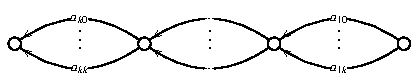
\includegraphics[width=0.92\textwidth]{figures/Fig_119_PDF222_Book210.pdf}
  \caption{$\mathbb P^k$ 上倾斜丛的箭图（原书 p.210）}
  \label{fig:tilting-projective-space-quiver}
\end{figure}
\end{example}

\begin{example}[带关系路径代数之间的倾斜]
不同的带关系路径代数也可以通过倾斜联系起来。最简单的例子是下图中的两个带关系箭图；后一个箭图是对象
\[
  T=S_2\oplus S_{23}\oplus P_2
\]
的自同态环（采用第\ref{subsec:linear-quiver}节所用记号）。
\begin{figure}[H]\centering
  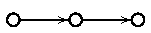
\includegraphics[width=0.31\textwidth]{figures/Fig_120_PDF223_Book211.pdf}\qquad
  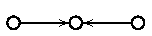
\includegraphics[width=0.31\textwidth]{figures/Fig_121_PDF223_Book211.pdf}
  \caption{倾斜前后的两个箭图（原书 p.211）}
  \label{fig:tilting-quiver-example}
\end{figure}
有限维代数的倾斜理论，更多内容参见\bookcite{10}。
\end{example}

\begin{note}\label{note:rarity-of-tilting-bundles}
\textbf{注 7.95.} 射影簇的相干层导出范畴有倾斜丛的情形相当少见。在一维时，只有射影直线有倾斜丛，其他曲线都没有；在二维时，有理曲面有倾斜丛\bookcite{120}。一般可以证明，若一个簇存在倾斜丛，则其 Grothendieck 群（见第\ref{ch:stability}章）是有限秩自由阿贝尔群。特别地，这排除了所有射影 Calabi--Yau 簇。
\end{note}

\subsection{矩阵分解与射影簇}\label{subsec:matrix-factorizations-projective-varieties}
设 $R=\mathbb C[X_0,\ldots,X_n]$，且 $f\in R$ 是次数为 $k$ 的齐次多项式。此时可以考虑两个范畴：
\begin{itemize}
  \item $X=\mathbb P(R/(f))$ 上相干层的导出范畴 $D\mathrm{Coh}^{\bullet}X$；
  \item 分次矩阵分解范畴 $\mathrm{grMF}^{\bullet}(R,f)$。
\end{itemize}
一般而言，这两个范畴并不等价，但彼此密切相关。

\begin{example}[三个齐次多项式的矩阵分解范畴]
考虑 $n=1$ 与三个函数
\[
  f_1=X,\qquad f_2=XY,\qquad f_3=XY(X-Y).
\]
簇 $X=\mathbb P(R/(f_k))$ 由 $k$ 个 $\mathbb P^1$ 上的点组成，且
\[
  X\subset\{(0:1),(1:0),(1:1)\}.
\]
因此 $X\cong V(\mathbb C^k)$，从而
\[
  D^b\mathrm{Coh}\,X\cong D^b\mathrm{mod}\,\mathbb C^k
  \cong D^b\mathrm{mod}\,\mathbb C Q,
\]
其中 $Q$ 是有 $k$ 个顶点且没有箭头的箭图。
\begin{itemize}
  \item 对 $f_1$，分次矩阵分解范畴是平凡的，因为 $V(R/(f_1))$ 是一条没有奇点的仿射直线。
  \item 对 $f_2$，范畴由下图所示的对象生成：
  \begin{figure}[H]\centering
    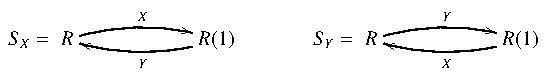
\includegraphics[width=0.78\textwidth]{figures/Fig_122_PDF223_Book211.pdf}
    \caption{$S_X$ 与 $S_Y$ 的矩阵分解（原书 p.211）}
    \label{fig:two-linear-matrix-factorizations}
  \end{figure}
  $S_X$ 与 $S_Y$ 的自同态环都同构于 $\mathbb C$，二者之间没有态射。因此
  \[
    \mathrm{grMF}^{\bullet}(R,f_2)\cong_\infty D\mathrm{mod}^{\bullet}\mathbb C Q,
  \]
  其中 $Q$ 是两个顶点且无箭头的箭图。
  \item 对 $f_3$，范畴由 $S_X(i),S_Y(i),S_{X-Y}(i)$ 生成。考察
  $S_X\oplus S_Y\oplus S_{X-Y}$ 的自同态代数，可见它同构于 $\mathbb C^3$。因此，这三个对象生成的子范畴与
  \[
    D\mathrm{mod}^{\bullet}\mathbb C^3
    \cong_\infty D\mathrm{Coh}^{\bullet}X
  \]
   等价；但这个子范畴并不等价于 $\mathrm{grMF}^{\bullet}(R,f_3)$。
% [Tutor Note: 原书此条（p.212）有两处把 $f_3$ 印成了 $f_2$：一是“$\mathrm{grMF}^{\bullet}(R,f_2)$ 中与 $D\mathrm{Coh}^{\bullet}X$ 等价的子范畴”，二是“不等价于 $\mathrm{grMF}^{\bullet}(R,f_2)$”。按上下文（本条讨论 $f_3=XY(X-Y)$，$f_2$ 的情形已在上一条处理）应为 $f_3$；译文已改。]
\end{itemize}
\end{example}

函数次数不同所导致的差异可以推广到所有射影空间的超曲面。

\begin{theorem}{Orlov 定理}{orlov-hypersurface}
设 $X=\mathbb P(R/(f))$ 是 $\mathbb P^n=\mathbb P(R)$ 中的光滑子簇，且 $k=\deg f$。则有以下函子：
\begin{enumerate}[label=(\roman*)]
  \item 若 $k<n+1$，则存在全忠实嵌入 $F\colon\mathrm{grMF}^{0}(R,f)\to D^b\mathrm{Coh}\,X$；
  \item 若 $k=n+1$，则存在等价 $F\colon D^b\mathrm{Coh}\,X\to\mathrm{grMF}^{0}(R,f)$；
  \item 若 $k>n+1$，则存在全忠实嵌入 $F\colon D^b\mathrm{Coh}\,X\to\mathrm{grMF}^{0}(R,f)$。
\end{enumerate}
\end{theorem}
\begin{proof}[证明思路]
涉及的两个范畴都可以构造为一个较大范畴的商：
\[
  D^b\mathrm{Coh}\,X\cong
  \frac{D^b\mathrm{grMod}\,R}{\langle\mathrm{grmod}\,R\rangle},
  \qquad
  \mathrm{grMF}^{0}(R,f)\cong
  \frac{D^b\mathrm{grMod}\,R}{\langle\mathrm{grProj}\,R\rangle}.
\]
两个分母分别是由有限维分次模和分次投射模生成的子范畴。在\bookcite{200}中，作者通过考察这两个子范畴在 $D^b\mathrm{grMod}\,R$ 中的相对位置，得到上述结论。

当 $k=n+1$ 时，Segal 与 Shipman\bookcite{216,225}还给出了一个漂亮的几何证明。把 $R$ 上的分次重新解释为群作用后，可以把 $\mathrm{grMF}(R,f)$ 看作商栈 $[\mathbb A^{n+1}/\mathbb Z_{n+1}]$ 上的矩阵分解范畴 $\mathrm{MF}([\mathbb A^{n+1}/\mathbb Z_{n+1}],f)$。这个栈与 $Y=|K_{\mathbb P^n}|$ 的典范丛全空间导出等价，因此可转而考察 $\mathrm{MF}(Y,f)$。在 $Y$ 上，$f$ 的零点由两部分组成：一部分是位于 $\mathbb P^n\subset |K_{\mathbb P^n}|=Y$ 中、在 $\mathbb P^n$ 上 $f$ 的零点之上的纤维，另一部分是 $\mathbb P^n$ 本身。因此奇点集为
\[
  X\subset\mathbb P^n\subset K_{\mathbb P^n}.
\]
局部而言，这是一个正规交，于是可用 Knörrer 周期性得到
\[
  \mathrm{MF}(Y,f)\simeq\mathrm{MF}(X,0)\cong D^b\mathrm{Coh}\,X.
\]
\end{proof}

\section{练习}\label{sec:exercises-chapter-seven}

\begin{exercise}\label{exer:varieties-same-finite-points}
设 $X_1,X_2$ 是两个仿射簇。
\begin{enumerate}[label=(\roman*)]
  \item 证明：若 $X_1,X_2$ 含有相同有限个点，则它们同构。
  \item 证明：若 $\mathrm{Coh}\,X_1\simeq\mathrm{Coh}\,X_2$，则 $X_1,X_2$ 同构（使用 Morita 等价）。
  \item 证明：对任意簇 $X$，有
  \[
    \mathcal O(X)\cong\operatorname{End}(1_{\mathrm{Perf}^{\bullet}X})
    \cong\operatorname{End}(1_{D\mathrm{Coh}^{\bullet}X}).
  \]
\end{enumerate}
\end{exercise}

\begin{exercise}\label{exer:product-varieties}
设 $X_1,X_2$ 是两个簇，分别有仿射开覆盖 $(U_{1,i})_i,(U_{2,j})_j$。把 $X_1\times X_2$ 看作由开集 $U_{1,i}\times U_{2,j}$ 覆盖的簇。
\begin{enumerate}[label=(\roman*)]
  \item 证明：若 $X_1=\mathbb P^n$、$X_2=\mathbb P^m$，则 $X_1\times X_2$ 可写成 $\mathbb P(R)$，其中 $R$ 是 $\mathbb C[X_0,\ldots,X_n,Y_0,\ldots,Y_m]$ 中由单项式 $X_iY_j$ 生成的子环。
  \item 令
  \[
    R=\mathbb C[X_1,\ldots,X_4]/(X_1^2+\cdots+X_4^2),\qquad \deg X_i=1.
  \]
  证明 $\mathbb P(R)$ 与 $\mathbb P^1\times\mathbb P^1$ 同构。
  \item 若 $M_1,M_2$ 分别是 $X_1,X_2$ 上的层，可在 $X_1\times X_2$ 上定义 $M_1\otimes M_2$，要求
  \[
    (M_1\otimes M_2)(U_{1,i}\times U_{2,j})
    =M_1(U_{1,i})\otimes M_2(U_{2,j}).
  \]
  证明：若 $M_1,M_2$ 局部自由，则 $M_1\otimes M_2$ 也局部自由。
\end{enumerate}
\end{exercise}

\begin{exercise}\label{exer:elliptic-curve-cohomology-and-generators}
令 $E=\mathbb P(R)$，其中
\[
  R=\mathbb C[X,Y,Z]/\bigl(Y^2Z-(X-\lambda_1Z)(X-\lambda_2Z)(X-\lambda_3Z)\bigr).
\]
\begin{enumerate}[label=(\roman*)]
  \item 证明 $E$ 光滑当且仅当 $\lambda_i$ 两两不同。以下各问均假设这一条件成立。
  \item 证明结构层的层上同调为 $\mathbb C\oplus\mathbb C$，分别集中在次数 $0,1$。
  \item 令 $S_p$ 是点 $p=(x:y:z)\in E$ 处的点层，构造它的局部自由分解。
  \item 利用该分解，计算 $D\mathrm{Coh}^{\bullet}E$ 中 $\mathcal O\oplus S_p$ 的自同态代数。证明该代数同构于下图箭图的路径代数模关系理想，其中关系为
  \begin{figure}[H]\centering
    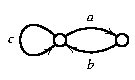
\includegraphics[width=0.27\textwidth]{figures/Fig_123_PDF225_Book213.pdf}
    \caption{练习 7.3(iv) 中的箭图（原书 p.213）}
    \label{fig:exercise-elliptic-endomorphism-quiver}
  \end{figure}
  \[
    \mathbb C Q/\langle ba,c^2\rangle.
  \]
  \item 可以证明 $\mathcal O$ 与 $S_p$ 分裂生成导出范畴。解释为什么这意味着 $\operatorname{End}(\mathcal O\oplus S_p)$ 上的 $A_\infty$ 结构必定非平凡。
\end{enumerate}
\end{exercise}

\begin{exercise}\label{exer:projective-hypersurface-smoothness}
令 $R=\mathbb C[X_0,\ldots,X_n]/(f)$，其中 $f$ 是次数为 $d$ 的不可约齐次函数。
\begin{enumerate}[label=(\roman*)]
  \item 证明 $V(R)$ 光滑当且仅当 $f$ 是线性的；此时 $V(R)\cong\mathbb A^n$。
  \item 证明：当 $d>1$ 时，对一般的 $f$，$\mathbb P(R)$ 光滑（也就是说，在所有次数为 $d$ 的齐次多项式组成的空间 $\mathbb C[X_0,\ldots,X_n]_d$ 中，光滑性构成一个稠密开条件）。
  \item 若 $\mathbb P(R)$ 光滑，证明 $K\cong\mathcal O(d-n-1)$；因此若 $d=n+1$，则 $\mathbb P(R)$ 是 Calabi--Yau 簇。
\end{enumerate}
\end{exercise}

\begin{exercise}\label{exer:quadric-surface-tilting}
令 $X=\mathbb P(R)$，其中
\[
  R=\mathbb C[X,Y,U,V]/(XY-UV),
\]
所有变量的次数均为 $1$。
\begin{enumerate}[label=(\roman*)]
  \item 求 $\mathrm{Perf}^{\bullet}X$ 中 $\mathcal O(0)\oplus\mathcal O(1)\oplus\mathcal O(2)\oplus\mathcal O(3)$ 的自同态环，并画出其箭图。
  \item 将 $X$ 识别为 $\mathbb P^1\times\mathbb P^1$。对每个 $(i,j)\in\mathbb Z^2$，定义
  \[
    \mathcal O(i,j)=\mathcal O_{\mathbb P^1}(i)\otimes\mathcal O_{\mathbb P^1}(j).
  \]
  求 $\mathcal O(0,0)\oplus\mathcal O(1,0)\oplus\mathcal O(0,1)\oplus\mathcal O(1,1)$ 的自同态环，并画出其箭图。
\end{enumerate}
\end{exercise}

\begin{exercise}\label{exer:matrix-factorizations-univariate}
令
\[
  f(X)=(X-\lambda_1)^{m_1}\cdots(X-\lambda_k)^{m_k}\in\mathbb C[X],
\]
并把指数向量记为 $\mathbf m$。对每个满足 $0\leq r_i\leq m_i$ 的序列 $\mathbf r=(r_i)$，有矩阵分解 $M_{\mathbf r}\in\mathrm{MF}^{\pm}(\mathbb C[X],f)$，对应于如下分解：
\[
  f=(X-\lambda_1)^{r_1}\cdots(X-\lambda_k)^{r_k}
  (X-\lambda_1)^{m_1-r_1}\cdots(X-\lambda_k)^{m_k-r_k}.
\]
\begin{enumerate}[label=(\roman*)]
  \item 证明 $M_{\mathbf r}$ 是零对象当且仅当 $\mathbf r=0$ 或 $\mathbf r=\mathbf m$。
  \item 证明
  \[
    M_{\mathbf r}\cong M_{(r_1,0,\ldots,0)}\oplus\cdots\oplus M_{(0,\ldots,0,r_k)}.
  \]
  \item 描述 $M_{\mathbf r}$ 的自同态环。
  \item 描述分次矩阵分解范畴 $\mathrm{grMF}^{\bullet}(\mathbb C[X],X^n)$。
\end{enumerate}
\end{exercise}

\begin{exercise}\label{exer:fourier-mukai-p1}
考察范畴 $D\mathrm{Coh}^{\bullet}\mathbb P^1$。
\begin{enumerate}[label=(\roman*)]
  \item 描述以点 $(p_1,p_2)\in\mathbb P^1\times\mathbb P^1$ 处的点层为核的 Fourier--Mukai 变换。
  \item 描述以线丛 $\mathcal O(i,j)=\mathcal O(i)\otimes\mathcal O(j)$ 为核的 Fourier--Mukai 变换。
  \item 求一个核，使相应的 Fourier--Mukai 变换对应于自同构
  \[
    \phi\colon\mathbb P^1\to\mathbb P^1,
    \qquad(x:y)\longmapsto(y:x)
  \]
  的（导出）拉回。
\end{enumerate}
\end{exercise}

\begin{exercise}\label{exer:calabi-yau-reconstruction}
Bondal--Orlov 定理说明，可以通过考察点型对象，从相干层导出范畴重构光滑 Fano 簇或一般型簇。点型对象是指其在导出范畴中的自同态代数为外代数 $\Lambda_n$ 的对象。这个想法在 Calabi--Yau 情形下并不奏效。
\begin{enumerate}[label=(\roman*)]
  \item 证明：对椭圆曲线
  \[
    E=\mathbb P(R),\qquad
    R=\mathbb C[X,Y,Z]/\bigl(Y^2Z-(X-\lambda_1Z)(X-\lambda_2Z)(X-\lambda_3Z)\bigr),
  \]
  线丛也都是点型对象。
  \item 举出一个 Fourier--Mukai 等价的例子，使其把点层变为线丛。
\end{enumerate}

一般而言，虽然不能从导出范畴重构 Calabi--Yau 簇，但对椭圆曲线仍可证明：若 $D\mathrm{Coh}^{\bullet}E_1\simeq D\mathrm{Coh}^{\bullet}E_2$，则 $E_1\cong E_2$。这是因为可以把 $E$ 重构为数值 Grothendieck 群中某个固定类的对象所组成的模空间（见\bookcite{205}）。
\end{exercise}

\begin{exercise}\label{exer:blowup-moduli-tilting}
原点 $(0,0)$ 处 $\mathbb A^2$ 的吹起是簇 $\widetilde{\mathbb A}^2:=\mathbb P(R)$，其中
\[
  R=\mathbb C[x,y,X,Y]/(Xy-xY),
\]
且 $x,y$ 的次数为 $0$，$X,Y$ 的次数为 $1$。
\begin{enumerate}[label=(\roman*)]
  \item 为 $\widetilde{\mathbb A}^2$ 找一个仿射开覆盖。
  \item 令 $Q$ 为下图所示的箭图。证明：维数向量 $\alpha=(1,1)$、稳定条件 $\theta=(-1,1)$ 对应的模空间是 $\widetilde{\mathbb A}^2$。
  \begin{figure}[H]\centering
    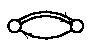
\includegraphics[width=0.26\textwidth]{figures/Fig_124_PDF227_Book215.pdf}
    \caption{练习 7.9(ii) 中的箭图（原书 p.215）}
    \label{fig:exercise-blowup-quiver}
  \end{figure}
  \item 证明相应的 $\widetilde{\mathbb A}^2$ 上的重言丛是一个倾斜丛。它的自同态环是什么？
\end{enumerate}
\end{exercise}

\begin{exercise}\label{exer:weighted-projective-line-stack}
考察带有群 $G=\{1,-1\}$ 作用的射影直线 $\mathbb P^1$，作用为
\[
  g\cdot(x:y)=(x:gy).
\]
加权射影直线 $\mathbb P^1_{2,2}$ 定义为商栈 $[\mathbb P^1/G]$。
\begin{enumerate}[label=(\roman*)]
  \item 定义 $\mathbb P^1_{2,2}$ 上 $G$-等变层的概念，并分类 $G$-等变线丛。令 $D\mathrm{Coh}^{\bullet}[\mathbb P^1/G]$ 表示 $G$-等变层的导出范畴。
  \item 将 $D\mathrm{Coh}^{\bullet}[\mathbb P^1/G]$ 解释为 $\mathbb P^1$ 上某个代数层的模所构成的导出范畴。
  \item 在 $D\mathrm{Coh}^{\bullet}[\mathbb P^1/G]$ 中寻找一个倾斜对象，并计算其自同态环。
\end{enumerate}
\end{exercise}

\chapterreview{%
\textbf{全章地位。}第 6 章用 Morse 理论造出 $A$ 侧的 $A_\infty$ 范畴，本章则用代数几何造出 $B$ 侧的相干层导出范畴与奇点范畴。作者避开消解与超上同调，改用仿射开集上的 Čech 复形直接给出 $A_\infty$ 增强，目的是让两侧范畴处在同一套语言里；第 8 至 10 章的镜像对应全部以 $D\mathrm{Coh}^{\bullet}X$ 为靶。

\textbf{知识脉络。}主线是“仿射环 $-$ 仿射簇反等价 $\to$ 模的层化 $\to$ 粘合成一般簇 $\to$ Čech 复形与层上同调 $\to$ 局部自由分解给出 $\mathrm{Perf}^{\bullet}X\subset D\mathrm{Coh}^{\bullet}X$”。§7.2 把机器推广到支撑层、概形、非交换簇、栈与 Landau--Ginzburg 模型；§7.3 反过来问导出范畴能记住多少几何：Fano 与反 Fano 簇可由 Serre 函子重构，一般簇之间的等价由 Fourier--Mukai 核给出，Orlov 定理说明这在光滑射影情形已完备；模空间与倾斜则把 $D\mathrm{Coh}^{\bullet}X$ 与箭图表示、$\mathrm{Perf}^{\bullet}A$ 联系起来。

\textbf{核心结论。}（1）仿射情形 $\mathrm{Perf}^{\bullet}X\cong_\infty D\mathrm{Proj}^{\bullet}R$，一般情形 $\mathrm{Perf}^{\bullet}X\subset D\mathrm{Coh}^{\bullet}X\subset D\mathrm{QCoh}^{\bullet}X$；$X$ 光滑当且仅当第一个包含是等价，也当且仅当 $D\mathrm{QCoh}^{\bullet}X$ 中 Hom 的次数有界。（2）矩阵分解由 $d_0d_1=d_1d_0=W$ 刻画：Knörrer 周期性给出 $\mathrm{MF}^{\pm}(R,W)\cong_\infty\mathrm{MF}^{\pm}(R[U,V],W+UV)$，孤立奇点情形由 Dyckerhoff 定理保证 $M_p$ 分裂生成，Buchweitz 定理把 $\mathrm{MF}^{0}(R,W)$ 等同于奇点范畴 $D^b\mathrm{Coh}X/\mathrm{Perf}X$。（3）仿射簇由 $\operatorname{End}(1_{D\mathrm{Coh}^{\bullet}X})\cong R$ 重构；Fano 或反 Fano 簇可由 Serre 函子 $-\otimes K[n]$ 重构。（4）核 $P\in D\mathrm{Coh}^{\bullet}(X\times Y)$ 给出 $\Phi_P=D\pi_{Y*}\circ(-\otimes P)\circ D\pi_X^*$，Orlov 定理断言光滑射影簇间的正合函子皆为此形；倾斜对象 $T$ 给出 $\mathcal C^{\bullet}\cong_\infty\mathrm{Perf}^{\bullet}A$，$A=\mathcal C^{\bullet}(T,T)$。

\textbf{辨析与提醒。}其一，$\bullet$ 记号不是装饰：$D\mathrm{Coh}^{\bullet}X$ 是 $A_\infty$ 增强，Hom 是复形而不仅是上同调群。其二，光滑性判据的方向要记清：光滑则每个相干层有有限局部自由分解，故 $\mathrm{Perf}=D\mathrm{Coh}$；有奇点时商 $D^b\mathrm{Coh}X/\mathrm{Perf}X$ 非零，它只探测奇点。其三，Serre 函子的自然同构方向极易写反，标准形式是 $\operatorname{Hom}(X,Y)\cong\operatorname{Hom}(Y,X\otimes K[n])^\vee$；Fourier--Mukai 的合成顺序同理，核在 $X\times Y$ 上决定函子 $X\to Y$，不能与转置核混为一谈。其四，$K^{-1}$ 丰富为 Fano、$K$ 丰富为反 Fano，方向只差一次对偶；“丰富”与“极丰富”也不同，后者要求 $L$ 本身给出射影嵌入。

\textbf{评注。}作者的取舍很明显：为与 $A$ 侧平行，他把层论压缩成“仿射覆盖 $+$ Čech 复形”，省略无界导出范畴的完备性、Brown 可表性与 Orlov 定理的证明；代价是补细节须另找文献，收益是 $B$ 侧范畴从第一页起就可计算。§7.2 把概形、栈与 LG 模型并置看似杂糅，实为第 8 章环簇与第 10 章镜像簇预置工具箱；矩阵分解若只当成 $\mathbb Z_2$ 玩具，就会错过它在分次理论中的核心地位。§7.3 揭示 $B$ 侧的刚性：Serre 函子把典范线丛变成范畴的内蕴对象，Fano 与反 Fano 因此可被范畴识别；到 Calabi--Yau 情形 $K$ 平凡，重构失效，镜像对应才真正开始。倾斜丛的存在性相当苛刻（例如所有射影 Calabi--Yau 簇都被排除），这也解释了作者为何把模空间与倾斜并置在末尾。阅读时宜与第 6 章对读：同一套 $A_\infty$ 语言，一侧由 Morse 轨迹给出，一侧由局部自由分解给出，这种对称是全书结构的主线。}

\chapter{镜像对称}
现在我们已经定义了与 $A$ 模型和 $B$ 模型相关的 $A_\infty$ 范畴，自然会提出一个问题：
\begin{center}
  \emph{是否能找到某些 $A$ 模型与 $B$ 模型，使它们描述同一个底层 $A_\infty$ 范畴？}
\end{center}
这一现象称为同调镜像对称。若一对 $A$ 模型与 $B$ 模型导出相同的范畴，就称它们为一对镜像。本章将讨论如何寻找可能的镜像对、如何证明它们互为镜像，并说明它们在几何上如何联系。

\section{复环面}\label{sec:complex-torus}
\takeaway{复环面 $T=(\mathbb C^*)^n$ 与 $T^*(S^1)^n$ 互为镜像：wrapped、正合、$\mathbb Z_2$ 分次三种 Fukaya 范畴分别等价于 $D\mathrm{Coh}^{\bullet}$、挠层与矩阵分解。镜像上的点对应底环面 $B$ 上的一维局部系统，因此 $T$ 的镜像是作为对偶群出现的 $T^\vee=\operatorname{Grp}(N,\mathbb C^*)$。}
我们从一个在第\ref{ch:physics-motivation}章已经研究过的例子开始。

\begin{example}[圆柱与复环面的镜像]
考察圆柱
\[
  X=T^*S^1\cong\mathbb C^*,
  \qquad \Omega=\frac{dz}{z},
\]
其中 $\Omega$ 是用于定义分次的体积形式。它可以看作带柱形端的 Liouville 流形。
\begin{itemize}
  \item 相应的 wrapped Fukaya 范畴 $\mathrm{wrFuk}^{\bullet}(X,\Omega)$ 由一个余切纤维生成，其自同态环为集中在次数 $0$ 的
  \[
    R=\mathbb C[X,X^{-1}].
  \]
  因而
  \[
    D^{\infty}\mathrm{wrFuk}^{\bullet}(T^*S^1,\Omega)
    =D^{\infty}R=D\mathrm{Mod}^{\bullet}R.
  \]
  后者与 $D\mathrm{Coh}^{\bullet}Y$ 同构，其中 $Y=V(R)\cong\mathbb C^*$。因此，$(T^*S^1,\mathbb C^*)$ 可以视为一对镜像：
  \[
    D^{\infty}\mathrm{wrFuk}^{\bullet}(T^*S^1,\Omega)
    \cong D\mathrm{Coh}^{\bullet}\mathbb C^*.
  \]
  \item 也可以考察 $T^*S^1$ 的正合 Fukaya 范畴。其对象是带局部系统的紧正合拉格朗日子流形。在同位变形意义下，这样的拉格朗日子流形只有圆周本身；局部系统可看成基本群
  \[
    \pi_1(S^1)=\mathbb Z
  \]
  的有限维表示，或其群环的有限维表示。该群环为
  \[
    \mathbb C[\pi_1(S^1)]\cong\mathbb C[X,X^{-1}]\cong R.
  \]
  于是有等价 $D\mathrm{mod}^{\bullet}R\simeq D\mathrm{Fuk}^{\bullet}X$。从 $B$ 侧看，$R$ 的有限维表示由 $Y=\mathbb C^*$ 上的点层 $S_p$ 生成；这些也称为挠层\index{naoceng@挠层|hyperpage}：
  \[
    D^{\infty}\mathrm{exFuk}^{\bullet}(T^*S^1,\Omega)
    =D^{\infty}\mathrm{tor}^{\bullet}\mathbb C^*
    :=\langle S_p\mid p\in\mathbb C^*\rangle
    \subset D\mathrm{Coh}^{\bullet}\mathbb C^*.
  \]
  \item 最后还可以考察 $\mathbb Z_2$ 分次的 wrapped Fukaya 范畴。它仍由一个余切纤维生成，所以与 $D^{\pm}R$ 等价。在 $B$ 侧，可以把这个范畴实现为矩阵分解范畴
  \[
    \mathrm{MF}^{\pm}(\mathbb C^3,(XY-1)Z).
  \]
  令 $F$ 表示 $\mathbb C[X,Y,Z]$ 上的秩一自由模。上述范畴由对象
  \[
    (F\oplus F,\begin{pmatrix}0&XY-1\\Z&0\end{pmatrix})
  \]
  生成；其自同态环为
  \[
    \mathbb C[X,Y,Z]/(XY-1,Z)\cong\mathbb C[X,X^{-1}]=R.
  \]
  从几何上看，这个 $B$ 模型对应于 $\mathbb C^3$ 中一个超曲面的奇点集；该超曲面由一个二次曲面与一个平面组成，二者的交是一条圆锥曲线，且同构于仿射簇 $\mathbb C^*$。因此
  \[
    D^{\infty}\mathrm{wrFuk}^{\pm}(T^*S^1)
    \simeq\mathrm{MF}^{\pm}(\mathbb C^3,(XY-1)Z).
  \]
\end{itemize}
所以，$\mathbb C^*$ 与 $T^*S^1$ 互为镜像这一事实，体现为三种不同的 $A_\infty$ 范畴等价。
\end{example}

上面的例子可以推广到高维。令
\[
  X=(T^*S^1)^n=T^*(S^1)^n,
  \qquad
  \Omega=\frac{dz_1}{z_1}\wedge\cdots\wedge\frac{dz_n}{z_n}.
\]
wrapped Fukaya 范畴仍由一个余切纤维分裂生成，但其自同态环变为
\[
  \mathbb C[X_1^{\pm1},\ldots,X_n^{\pm1}],
\]
对应的仿射簇为 $(\mathbb C^*)^n$。因此，$(T^*(S^1)^n,(\mathbb C^*)^n)$ 是一对镜像。

底空间 $L=(S^1)^n$ 是 $X$ 中的正合拉格朗日环面。由第\ref{ch:physics-motivation}章可知，给 $L$ 配备平凡局部系统时，其自同态环是环面的上同调环，也就是 $n$ 个变量生成的外代数 $\Lambda_n$。在 $L$ 上选取非平凡局部系统，相当于选择基本群 $\pi_1(L)=\mathbb Z^n$ 的一个表示。这个基本群的群环为
\[
  \mathbb C[X_1^{\pm1},\ldots,X_n^{\pm1}],
\]
故其每个有限维模都给出正合 Fukaya 范畴的一个对象。从 $B$ 侧看，一维简单模对应于
\[
  V\bigl(\mathbb C[X_1^{\pm1},\ldots,X_n^{\pm1}]\bigr)\cong(\mathbb C^*)^n
\]
上的点层。一般而言，坐标环的有限维模所对应的层也称为挠层。无分次版本也可以推广，于是得到下列等价表：
\[
\begin{array}{c|c|c}
\text{$A$ 模型} & \text{代数} & \text{$B$ 模型}\\\hline
D^{\infty}\mathrm{wrFuk}^{\bullet}(T^*(S^1)^n,\Omega)
 &D\mathrm{Mod}^{\bullet}\mathbb C[X_1^{\pm1},\ldots,X_n^{\pm1}]
 &D\mathrm{Coh}^{\bullet}(\mathbb C^*)^n\\
D^{\infty}\mathrm{exFuk}^{\bullet}(T^*(S^1)^n,\Omega)
 &D\mathrm{mod}^{\bullet}\mathbb C[X_1^{\pm1},\ldots,X_n^{\pm1}]
 &D\mathrm{tor}^{\bullet}(\mathbb C^*)^n\\
D^{\infty}\mathrm{wrFuk}^{\pm}(T^*(S^1)^n)
 &D^{\pm}\mathbb C[X_1^{\pm1},\ldots,X_n^{\pm1}]
 &\mathrm{MF}^{\pm}(\mathbb C^{n+2},(X_0\cdots X_n-1)Z)
\end{array}
\]

在上面的例子中，$X=T^*(S^1)^n\cong(\mathbb C^*)^n$ 与 $Y=(\mathbb C^*)^n$ 互为镜像，而 $Y$ 又与 $X$ 同构。这种看法有些迷惑性，因为实际上不应把 $X$ 与 $Y$ 看作同一个空间；它们是对偶的。

乘法群 $(\mathbb C^*)^n$ 称为 $n$ 维复环面，记为 $T$。与之相关的还有两个群：特征群\index{tezhengqun@特征群|hyperpage}
\[
  M:=\operatorname{Grp}(T,\mathbb C^*)
\]
和单参数子群所成的群
\[
  N:=\operatorname{Grp}(\mathbb C^*,T).
\]
二者都同构于 $\mathbb Z^n$。对每个 $u,v\in\mathbb Z^n$，定义
\[
  \chi_u\colon T\to\mathbb C^*,\quad
  (x_1,\ldots,x_n)\longmapsto x_1^{u_1}\cdots x_n^{u_n}\in M,
\]
和
\[
  \lambda_v\colon\mathbb C^*\to T,\quad
  t\longmapsto(t^{v_1},\ldots,t^{v_n})\in N.
\]
这两个群通过自然配对互为对偶：
\[
  \langle u,v\rangle=u_1v_1+\cdots+u_nv_n,
  \qquad \chi_u\circ\lambda_v(t)=t^{\langle u,v\rangle}.
\]
我们可以把 $T$ 重构为 $\operatorname{Grp}(M,\mathbb C^*)$ 或 $V(\mathbb C[M])$，因此定义对偶环面
\[
  T^\vee:=\operatorname{Grp}(N,\mathbb C^*)=V(\mathbb C[N]).
\]
% [Tutor Note: 配对 $\langle u,v\rangle=\sum u_iv_i$ 中 $u\in M$ 是“频率”（出现在单项式指数上），$v\in N$ 是“周期”（单参数子群的生成方向）；$\chi_u\circ\lambda_v(t)=t^{\langle u,v\rangle}$ 说两者相乘才给出数。把 $M,N$ 都识别成 $\mathbb Z^n$ 之后极易把指标写反：本节的射线向量住在 $N$，而对偶锥与势函数的单项式指数住在 $M$。]

回忆一下，$X=T^*(S^1)^n=T$ 的镜像上的点，对应于底空间
\[
  B=\{x\in T\mid|x|=1\}=(S^1)^n
\]
上的一维局部系统；等价地，对应于其基本群的一维表示。这个基本群可以认作 $N$：每个 $\lambda_v$ 都给出一个环路
\[
  \ell_v\colon[0,1]\to B,\qquad
  s\longmapsto\lambda_v(e^{2\pi is}).
\]
因此，$T$ 的镜像自然地可视为
\[
  \operatorname{Hom}(N,\mathbb C^*)=T^\vee.
\]
这一观察将成为我们寻找其他镜像对\index{jingxiangdui@镜像对|hyperpage}的出发点。

\section{环簇}\label{sec:toric-varieties}
\takeaway{环簇由扇（整锥的集合）组合地定义，锥与环面轨道一一对应且 $\dim\sigma=n-\dim O_\sigma$；每个环簇除子 $D_\sigma$ 对应 $B$ 侧势函数中的单项式 $y^{v_\sigma}$，由此猜测 $(X_\Delta,\sum D_\sigma)$ 的镜像是 Landau--Ginzburg 模型 $(T^\vee,W_\hbar)$。}
将镜像对称推广到复环面\index{fuhuanmian@复环面|hyperpage}之外的一种方法，是考察环簇\index{huanzu@环簇|hyperpage}（toric variety）。这类簇以复环面为稠密开子集，并且可以由组合数据定义。环簇理论发展成熟，包含代数几何中许多重要概念的说明性例子。更多内容参见\bookcite{89,57}。

令 $T,T^\vee$ 为上一节中的对偶环面\index{duiouhuanmian@对偶环面|hyperpage}。相应的对偶格记为
\[
  M=\operatorname{Hom}(T,\mathbb C^*)=\operatorname{Hom}(\mathbb C^*,T^\vee),
  \qquad
  N=\operatorname{Hom}(T^\vee,\mathbb C^*)=\operatorname{Hom}(\mathbb C^*,T),
\]
并记 $M_{\mathbb R}=M\otimes_{\mathbb Z}\mathbb R$、$N_{\mathbb R}=N\otimes_{\mathbb Z}\mathbb R$。格与相应实向量空间之间的自然配对记为 $\langle\ ,\ \rangle$。把 $M,N$ 识别为 $\mathbb Z^n$，把 $M_{\mathbb R},N_{\mathbb R}$ 识别为 $\mathbb R^n$，使得该配对就是标准内积。

坐标环 $\mathcal O(T)$ 同构于群环
\[
  \mathbb C[M]=\mathbb C[X_1^{\pm1},\ldots,X_n^{\pm1}].
\]
当 $u\in M=\mathbb Z^n$ 时，把单项式 $X_1^{u_1}\cdots X_n^{u_n}$ 简记为 $X^u$。类似地，
\[
  \mathcal O(T^\vee)=\mathbb C[N]\cong\mathbb C[Y_1^{\pm1},\ldots,Y_n^{\pm1}],
\]
并把与 $v\in N=\mathbb Z^n$ 对应的单项式记作 $Y^v$。

\begin{definition}{整锥}{integral-cone}
$N_{\mathbb R}$ 中的整锥\index{zhengzhui@整锥|hyperpage}是形如
\[
  \sigma=\{\lambda_1v_1+\cdots+\lambda_kv_k\mid
  \lambda_i\in\mathbb R_{\geq0}\}\subset N_{\mathbb R},
  \qquad v_i\in N
\]
的子集。每个锥都有对偶锥\index{duiouzhui@对偶锥|hyperpage}
\[
  \sigma^\vee:=\{u\in M_{\mathbb R}\mid
  \text{对所有 }v\in\sigma,\ \langle u,v\rangle\geq0\}.
\]
对每个 $u\in\sigma^\vee$，还可定义
\[
  \tau_u:=\{v\in\sigma\mid\langle u,v\rangle=0\}.
\]
这些集合仍是整锥，称为 $\sigma$ 的面\index{zhuidemian@锥的面|hyperpage}。
\end{definition}

\begin{definition}{扇}{fan}
扇\index{shan@扇|hyperpage} $\Delta$ 是 $N_{\mathbb R}$ 中整锥构成的集合，并满足：
\begin{itemize}
  \item 若 $\sigma\in\Delta$，且 $\tau$ 是 $\sigma$ 的一个面，则 $\tau\in\Delta$；
  \item 若 $\sigma_1,\sigma_2\in\Delta$，则 $\sigma_1\cap\sigma_2$ 是二者的公共面。
\end{itemize}
$\Delta$ 中所有 $k$ 维锥组成的子集记为 $\Delta_k$。
\end{definition}

扇是一种可用来定义簇的组合数据。每个锥定义群环 $\mathbb C[M]$ 的一个仿射子环
\[
  R_\sigma=\mathbb C[\sigma^\vee\cap M]
  =\mathbb C[X^u\mid u\in\sigma^\vee\cap M],
\]
和仿射簇 $U_\sigma=V(R_\sigma)$。若 $\tau_u$ 是 $\sigma$ 的一个面，则
\[
  \tau_u^\vee=\sigma^\vee+\mathbb R u,
  \qquad R_{\tau_u}=R_\sigma[X^{-u}],
\]
所以 $R_{\tau_u}$ 是 $R_\sigma$ 的局部化。从几何上看，$U_{\tau_u}$ 是 $U_\sigma$ 的开子集。若两个锥 $\sigma_1,\sigma_2$ 有公共面 $\tau$，就可沿图表
\[
  U_{\sigma_1}\longleftarrow U_\tau\longrightarrow U_{\sigma_2}
\]
将它们粘合起来。对扇中的所有锥都这样处理，便得到一个簇。

\begin{definition}{扇所确定的环簇}{toric-variety-from-fan}
簇
\[
  X_\Delta:=\bigcup_{\sigma\in\Delta}U_\sigma
\]
称为与扇 $\Delta$ 对应的环簇。
\end{definition}

\begin{example}[射影平面对应的扇]
令 $N=\mathbb Z^2$，取
\[
  v_1=(1,0),\qquad v_2=(0,1),\qquad v_3=(-1,-1),
\]
并令 $\sigma_i=\mathbb R_{\geq0}v_j+\mathbb R_{\geq0}v_k$，其中 $\{i,j,k\}=\{1,2,3\}$。再令
\[
  \tau_i=\mathbb R_{\geq0}v_i=\sigma_j\cap\sigma_k,
\]
注意 $\sigma_1\cap\sigma_2\cap\sigma_3=\{0\}$。集合
\[
  \Delta=\{\sigma_1,\sigma_2,\sigma_3,\tau_1,\tau_2,\tau_3,\{0\}\}
\]
是一个扇。相应的环为
\[
  R_{\sigma_1}=\mathbb C[YX^{-1},X^{-1}],\quad
  R_{\sigma_2}=\mathbb C[XY^{-1},Y^{-1}],\quad
  R_{\sigma_3}=\mathbb C[X,Y].
\]
这些都是多项式环，所以 $U_{\sigma_i}$ 都同构于 $\mathbb A^2=\mathbb C^2$。它们通过过渡映射粘合；这些映射与射影平面中三个标准仿射平面间的过渡映射一致：
\begin{figure}[H]\centering
  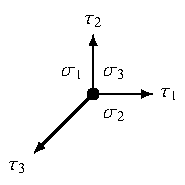
\includegraphics[width=0.37\textwidth]{figures/Fig_125_PDF232_Book220.pdf}
  \caption{射影平面对应的扇（原书 p.220）}
  \label{fig:fan-projective-plane}
\end{figure}
三个仿射片的坐标与齐次坐标之间的变换为
\[
\begin{array}{c|ccc}
 & U_{\sigma_3} & U_{\sigma_2} & U_{\sigma_1} \\ 
X_\Delta & (x,y) & (xy^{-1},y^{-1}) & (yx^{-1},x^{-1}) \\ 
\mathbb P^2 & (x:y:1) & (xy^{-1}:1:y^{-1}) & (1:yx^{-1}:x^{-1})
\end{array}
\]
这些正是射影平面中三个标准仿射片的过渡映射，因此 $X_\Delta\cong\mathbb P^2$。
\end{example}

因为所有环 $R_\sigma$ 都包含在 $\mathbb C[M]$ 中，每个仿射开集 $U_\sigma$ 都包含 $V(\mathbb C[M])=T$。这个开子集是稠密的，并且是群 $G=\mathbb C^{*n}\cong T$ 的一个轨道。$G$ 在各个 $R_\sigma$ 上的作用诱导了 $X_\Delta$ 上的作用，其形式为
\[
  g\cdot X^u=g_1^{u_1}\cdots g_n^{u_n}X^u.
\]
反过来，环簇也可以从这种几何性质刻画。

\begin{theorem}{环簇的扇刻画}{toric-variety-fan-classification}
每个 $n$ 维正规簇 $X$，只要带有 $T=(\mathbb C^*)^n$ 的忠实作用且存在稠密轨道，就来自某个扇 $\Delta$。锥 $\sigma\in\Delta$ 与轨道 $O_\sigma\in X/T$ 一一对应，且
\[
  \dim\sigma=n-\dim O_\sigma.
\]
\end{theorem}
\begin{proof}[证明思路]
固定稠密环面轨道中的一点 $p$。令 $N_+$ 为所有单参数子群\index{dancanshuqun@单参数子群|hyperpage} $\lambda_v\in\operatorname{Grp}(\mathbb C^*,T)$ 所成的集合，其中 $\lim_{t\to0}\lambda_v(t)p$ 在 $X$ 中存在。在 $N_+$ 上定义等价关系：若两个单参数子群给出同一个 $T$-轨道中的极限点，就称它们等价。这个等价关系把 $N_+$ 分成若干等价类 $E$，每个类对应一个轨道。对每个类，取其中向量的所有非负线性组合所成集合的闭包：
\[
  \sigma_E=\overline{\left\{\sum_i\lambda_i v_i\mid
  \lambda_i\in\mathbb R_{\geq0},\ v_i\in E\right\}}.
\]
这些是锥，且全体 $\sigma_E$ 构成所需的扇。为证明 $X_\Delta\cong X$，可构造一个环面等变态射，把 $X_\Delta$ 稠密环面中的一点 $q$ 映到 $p$。由于 $p$ 的轨道在 $X$ 中稠密，该态射是满射；由 $X$ 的正规性可推出它是单射。轨道与锥之间对应关系的更多细节，参见\bookcite[第 3.1 节]{89}。
\end{proof}
% [Tutor Note: “由正规性推出单射”省略的是 Zariski 主定理：正规簇之间的双有理、纤维有限的态射是开浸入；这里轨道分解说明该态射双有理且纤维有限，再加满射即为同构。若 $X$ 不正规，同一个扇给出的映射仍满射，但可能把若干轨道压到同一点，锥与轨道的双射即失效。]

\begin{example}[仿射平面对应的扇]
考察 $\mathbb A^2$，令 $g=(g_1,g_2)\in\mathbb C^*\times\mathbb C^*$ 通过
\[
  g\cdot(x,y)=(g_1x,g_2y)
\]
作用。固定稠密环面 $\mathbb C^*\times\mathbb C^*\subset\mathbb A^2$ 中的点 $(1,1)$。当且仅当 $k_1,k_2\geq0$ 时，极限
\[
  \lim_{t\to0}(t^{k_1},t^{k_2})
\]
存在，因此 $N_+=\mathbb Z_{\geq0}\times\mathbb Z_{\geq0}$。它分成四个等价类：
\[
  \{(0,0)\},\quad \{0\}\times\mathbb Z_{>0},\quad
  \mathbb Z_{>0}\times\{0\},\quad \mathbb Z_{>0}\times\mathbb Z_{>0},
\]
分别对应极限点 $(1,1),(1,0),(0,1),(0,0)$。
\begin{figure}[H]\centering
  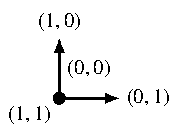
\includegraphics[width=0.25\textwidth]{figures/Fig_126_PDF233_Book221.pdf}
  \caption{仿射平面的扇及轨道极限（原书 p.221）}
  \label{fig:affine-plane-fan-orbits}
\end{figure}
相应的扇为
\[
  \Delta=\{\{(0,0)\},\ \{0\}\times\mathbb R_{\geq0},\
  \mathbb R_{\geq0}\times\{0\},\ \mathbb R_{\geq0}\times\mathbb R_{\geq0}\}.
\]
\end{example}

设 $T=\mathbb C^{*n}$，且 $\pi\colon\widetilde X\to X$ 是环簇之间的满射环面等变态射，并满足 $\pi|_T=1_T$。若两个单参数子群在 $\widetilde X$ 中等价，那么它们在 $X$ 中也等价；因此 $\widetilde X$ 中的锥是 $X$ 中锥的子锥，亦即 $\widetilde X$ 的扇是对 $X$ 的扇作细分所得。反过来，把一个扇细分成更小的锥，会得到一个映到原环簇上的新环簇。

\begin{example}[仿射平面的爆破]
最简单的例子是把仿射平面的锥细分成两个锥：
\begin{figure}[H]\centering
  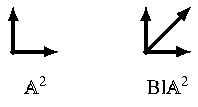
\includegraphics[width=0.36\textwidth]{figures/Fig_127_PDF233_Book221.pdf}
  \caption{$\mathbb A^2$ 的爆破（原书 p.221）}
  \label{fig:blowup-affine-plane-fan}
\end{figure}
在 $\mathbb A^2$ 中，二维锥对应于零轨道。在 $\mathrm{Bl}_0\mathbb A^2$ 中，这个锥被细分为三个锥：两个二维锥各对应一个零维轨道，一个一维锥对应一个一维轨道，该轨道同构于 $\mathbb C^*$。这些轨道合起来构成一条映到原点的 $\mathbb P^1$。换言之，我们把 $\mathbb A^2$ 的原点爆破成一条射影直线。
\end{example}

\begin{example}[$A_{k-1}$ 奇点]\label{ex:ak-singularity-resolution}
考察 $\mathbb R^2$ 中的扇 $\Delta$，其中唯一的二维锥为
\[
  \sigma=\mathbb R_{\geq0}(1,0)+\mathbb R_{\geq0}(1,k).
\]
其对偶锥为
\[
  \sigma^\vee=\mathbb R_{\geq0}(0,1)+\mathbb R_{\geq0}(k,-1),
\]
因此
\[
  \begin{aligned}
  \mathbb C[U_\sigma]
  &=\mathbb C[X^iY^j\mid i\geq0,\ i+kj\geq0]\\
  &=\mathbb C[X^kY^{-1},Y,X]
   \cong\mathbb C[U,V,W]/(UV-W^k).
  \end{aligned}
\]
这个环也是群 $G=\langle g\mid g^k=1\rangle\cong\mathbb Z/k\mathbb Z$ 在 $\mathbb C^2$ 上作用的不变量环，其中
\[
  g(x,y)=(\zeta x,\zeta^{-1}y),
\]
$\zeta$ 是 $k$ 次本原单位根。因此，$X_\Delta$ 同构于仿射商 $\mathbb C^2//G$，而与 $\sigma$ 对应的零维环面轨道就是奇点。

在锥 $\sigma$ 中加入方向为 $v_\ell=(1,\ell)$（$0<\ell<k$）的射线，就可以把 $\sigma$ 细分为 $k$ 个更小的锥。新扇的二维锥为
\[
  \sigma_\ell=\mathbb R_{\geq0}(1,\ell)
  +\mathbb R_{\geq0}(1,\ell+1),\qquad 0\leq\ell<k.
\]
容易验证，对所有 $\ell$，都有 $\mathbb C[U_{\sigma_\ell}]\cong\mathbb C[X,Y]$，所以新的环簇 $\widetilde X$ 是光滑的。
\begin{figure}[H]\centering
  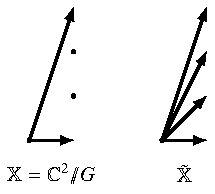
\includegraphics[width=0.54\textwidth]{figures/Fig_128_PDF234_Book222.pdf}
  \caption{$A_{k-1}$ 奇点及其消解（原书 p.222）}
  \label{fig:ak-singularity-resolution}
\end{figure}
每条新增射线给出一个同构于 $\mathbb C^*$ 的环面轨道，每个 $\sigma_\ell$ 给出一个零维环面轨道。它们合起来形成一串 $\mathbb P^1$，在投影映射 $\pi\colon\widetilde X\to X$ 下映到奇点。映射 $\pi$ 称为 $X$ 的一个奇点消解\index{qidianjiexiao@奇点消解|hyperpage}：它是满射、真映射、几乎处处一一对应，并且定义域 $\widetilde X$ 光滑。
\end{example}

前面的定理与例子说明，环簇中的环面轨道与扇的锥一一对应。稠密环面轨道对应零锥，一维锥对应 $(n-1)$ 维轨道。对每个一维锥 $\sigma$，可以定义两个对象：
\begin{itemize}
  \item 射线向量\index{shexianxiangliang@射线向量|hyperpage} $v_\sigma$，即半群 $\sigma\cap N$ 的生成元（最小非零格向量）；
  \item 环簇除子\index{huanzuchuzi@环簇除子|hyperpage} $D_\sigma$，即轨道 $O_\sigma$ 的闭包。
\end{itemize}
后者是一个 $(n-1)$ 维子簇，由所有锥包含 $v_\sigma$ 的轨道组成。由于每个非零锥至少包含一条射线，稠密环面的补集就是所有环簇除子的并：
\[
  X_\Delta\setminus T=\bigcup_{\sigma\in\Delta_1}D_\sigma.
\]

以上观察使我们得以初步猜测环簇的镜像是什么。考虑相对 Fukaya 范畴 $\mathrm{cuFuk}^{\pm}(X_\Delta,D)$，其中
\[
  D=\sum_{\sigma\in\Delta_1}D_\sigma
\]
是所有环簇除子的和。这个范畴是定义在形式幂级数环 $\mathbb C[[\hbar]]$ 上的带曲率形变，其未形变部分是环面 $T$ 的正合 Fukaya 范畴 $\mathrm{exFuk}^{\pm}(T)$。其对象为正合 Fukaya 范畴中的一对 $(L,\rho)$，其中
\[
  L=(S^1)^n\subset\mathbb C^{*n}=T^*(S^1)^n
\]
是拉格朗日基环面，$\rho$ 是基本群
\[
  \pi_1(L)=\pi_1(T)=N
\]
的一个表示。若 $\rho$ 是一维表示，则 $(L,\rho)$ 可认作
\[
  \operatorname{Hom}(N,\mathbb C^*)=T^\vee
\]
中的一点。把该点记作
\[
  (y_1,\ldots,y_n)=(\rho(\ell_1),\ldots,\rho(\ell_n))\in T^\vee,
\]
其中 $\ell_i$ 是 $N=\pi_1(L)=\mathbb Z^n$ 标准基所对应的环路。

将曲率打开，转到相对 Fukaya 范畴时会发生什么？若 $v=v_\sigma$ 是除子 $D_\sigma$ 的射线向量，就可考虑相应的单参数子群
\[
  \lambda_v\colon\mathbb C^*\to T.
\]
由于其在 $t\to0$ 时的极限存在于 $X_\Delta$ 中，$\lambda_v$ 在圆盘 $D\subset\mathbb C$ 上的延拓与限制定义了一张边界落在 $L$ 上、并与 $D_\sigma$ 相交的全纯圆盘。对对象 $(L,\rho)$ 而言，这张全纯圆盘对 $\mu^0$ 的贡献中出现因子
\[
  \rho(\lambda_v|_{S^1})\,\hbar.
\]
其中 $\rho(\lambda_v|_{S^1})$ 来自沿圆盘边界的平行移动，而 $\hbar$ 记录与除子的相交。从镜像一侧看，这意味着每个点 $y=(y_1,\ldots,y_n)\in T^\vee$ 都带有曲率 $W_\hbar(y)$，其中
\[
  W_\hbar=\sum_{\sigma\in\Delta_1}\hbar\,y^{v_\sigma}.
\]
注意，$\mu^0$ 还可能有其他贡献，$\mu^{>0}$ 也可能有贡献；但若运气好，我们找出的这些贡献就足以确定形变的同构类。这提示我们，$(X_\Delta,D)$ 的 $A$ 模型在 $B$ 侧的镜像可能是 Landau--Ginzburg 模型 $(T^\vee,W_\hbar)$。

\begin{note}\label{note:toric-divisor-potential}
\textbf{观察 8.10.} 在 $A$ 模型中加入环簇除子 $D_v$，会在 $B$ 模型的势函数中加入对偶单项式 $y^v$（也可能同时出现其他形变项）。
\end{note}

环簇除子与单项式项的对应关系似乎也可反向使用。回看例\ref{ex:punctured-plane-lg-model}和例\ref{ex:lefschetz-cylinder-quiver}，可见在 $A$ 模型中引入单项式项 $x,x^{-1}$，会得到一个与 $D\mathrm{mod}^{\bullet}\mathbb C Q_3^+$ 等价的有向 Fukaya 范畴。在第\ref{subsec:kronecker-quiver-sheaves}节中我们看到，这与 $\mathbb P^1$ 的导出范畴等价。$\mathbb P^1$ 是一个一维环簇，对应于扇
\[
  \Delta=\{0,\mathbb R_{\geq0},\mathbb R_{\leq0},\mathbb R\},
\]
其两个环簇除子为 $D_{+1}=\{0\}$、$D_{-1}=\{\infty\}$，相应的射线向量为 $N$ 中的 $\pm1$。

\begin{figure}[H]\centering
  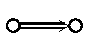
\includegraphics[width=0.33\textwidth]{figures/Fig_129_PDF235_Book223.pdf}
  \caption{有向 Fukaya 范畴中的两个生成对象（原书 p.223）}
  \label{fig:two-arrow-quiver}
\end{figure}
上图中的两个对象与 $\mathbb P^1$ 的两个环簇除子相对应。其扇由一维格 $N\cong\mathbb Z$ 中的两条射线及其交集构成：
\begin{figure}[H]\centering
  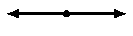
\includegraphics[width=0.22\textwidth]{figures/Fig_130_PDF235_Book223.pdf}
  \caption{$\mathbb P^1$ 的扇（原书 p.223）}
  \label{fig:fan-projective-line}
\end{figure}

\begin{note}\label{note:monomial-toric-divisor}
\textbf{观察 8.11.} 在 $A$ 模型的势函数中加入单项式项 $y^v$，对应于在 $B$ 模型中引入环簇除子 $D_v$。
\end{note}

请注意，目前这些观察还只是一些猜想性的提示，说明 $A$ 模型与 $B$ 模型之间可能如何关联。要得到更精确的结论，我们还需要引入另一种几何。

\section{热带几何}\label{sec:tropical-geometry}
\takeaway{令 $t\to\infty$，超曲面 $W_t^{-1}(0)$ 的阿米巴收缩为热带超曲面 $H_{\mathrm{trop}}$，后者是分段线性函数 $W_{\mathrm{trop}}=\max_m\lambda_m$ 不光滑的轨迹；热带曲线的腿数与亏格分别等于 Newton 多边形的边界格点数与内部格点数，并给出 $\square$ 的对偶三角剖分。}
Landau--Ginzburg 模型由一个带全纯函数的簇 $(Y,W)$ 构成。正如上一节所见，我们尤其关心簇为对偶环面 $T^\vee$、且势函数
\[
  W_\hbar\colon T^\vee\to\mathbb C
\]
依赖形变参数 $\hbar$ 的情形。一般而言，$A$ 模型 $(Y,W)$ 并不依赖 $\hbar$；因此我们将考察 $\hbar\to0$ 时的情形，或者等价地，令参数 $t=\hbar^{-1}$ 趋于无穷。这会引出一种称为热带几何的新几何。该领域的综述可参见 Mikhalkin\bookcite{175}，入门专著可参见 Maclagan 与 Sturmfels\bookcite{181}。

考虑一族 Laurent 多项式
\[
  W_t\in\mathbb C[Y_1^{\pm1},\ldots,Y_n^{\pm1},t^{\pm1}],
\]
并考察给定 $t\in\mathbb R_{>0}$ 时，对偶环面 $T^\vee$ 中由 $W_t$ 定义的超曲面。这类超曲面的拓扑不总是容易可视化，但可以通过阿米巴\index{amiba@阿米巴|hyperpage}来研究。\footnote{阿米巴（amoeba，源自希腊语“变形虫”）是复环面中超曲面在逐坐标对数映射下的像；它通常呈一只带腿的厚实变形虫之形，故得名。这一概念由 Gelfand、Kapranov 与 Zelevinsky 引入\bookcite{106}，其后在热带几何的研究中得到发展\bookcite{86,175}。}

\begin{definition}{Gelfand--Zelevinsky--Kapranov\bookcite{106}}{rescaled-amoeba}
定义映射
\[
  \log_t\colon T^\vee\to\mathbb R^n,
  \qquad (y_1,\ldots,y_n)\longmapsto
  \frac{1}{\ln|t|}(\ln|y_1|,\ldots,\ln|y_n|).
\]
$W_t$ 的（缩放）阿米巴是 $W_t^{-1}(0)$ 在此对数映射下的像：
\[
  A_t:=\log_t\{(y_1,\ldots,y_n)\in\mathbb C^{*n}\mid
  W_t(y_1,\ldots,y_n)=0\}.
\]
\end{definition}

\begin{example}[一个 Laurent 多项式的阿米巴]
取 $t=2$，令
\[
  W_t=X^2Y^3+X^2Y^2+tX^2Y-5XY^2+3XY-Y^2+t^2Y+1.
\]
它的阿米巴是由下图中的弯曲曲线围成的区域。
\begin{figure}[H]\centering
  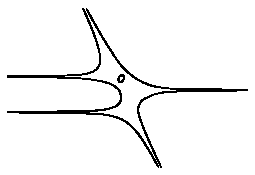
\includegraphics[width=0.53\textwidth]{figures/Fig_131_PDF236_Book224.pdf}
  \caption{例 8.13 中 Laurent 多项式的阿米巴（原书 p.224）}
  \label{fig:amoeba-example-813}
\end{figure}
\end{example}

一般而言，$\mathbb C^{*2}$ 中超曲面的阿米巴看起来像一张加厚的分段线性图，带有若干条无限延伸的腿。令 $t$ 趋于无穷时，这层加厚会逐渐收缩，极限就是那张图。

为精确说明这一点，把
\[
  W_t=\sum_{m\in M}c_m t^{k_m}Y^m
\]
写成单项式之和，其中指数 $m\in M\subset\mathbb Z^n$，系数由 $c_m\in\mathbb C^*$ 与 $t$ 的整数次幂 $k_m\in\mathbb Z$ 构成。令 $t$ 趋于无穷时，阿米巴 $A_t$ 趋近某个多面体骨架。原因是当 $t$ 很大时，在大多数点上，$W_t(y)$ 的某个单项式会占主导，因此 $W_t(y)\ne0$。只有当两个单项式大小相等时，它们才可能相消而使总和为零。每个单项式 $c_mt^{k_m}Y^m$ 定义线性函数
\[
  \lambda_m\colon\mathbb R^n\to\mathbb R,
  \qquad u\longmapsto\langle u,m\rangle+k_m.
\]
因此，$A_t$ 中的点集中在最大值同时由至少两个函数 $\lambda_m$ 取得的位置附近。

\begin{definition}{热带函数与热带超曲面}{tropical-function-hypersurface}
设 $W_t=\sum_{m\in M}c_mt^{k_m}Y^m$，其对应的热带函数\index{redaihanshu@热带函数|hyperpage}为
\[
  W_{\mathrm{trop}}\colon\mathbb R^n\to\mathbb R,
  \qquad u\longmapsto\max_{m\in M}\lambda_m(u).
\]
它是 $\mathbb R^n$ 上的分段线性函数，并把 $\mathbb R^n$ 分成若干胞腔 $\overline B_m$；在 $\overline B_m$ 上，$W_{\mathrm{trop}}$ 等于与单项式 $m$ 对应的线性函数 $\lambda_m$。热带超曲面\index{redaichaoqumian@热带超曲面|hyperpage} $H_{\mathrm{trop}}$ 是 $W_{\mathrm{trop}}$ 不光滑的轨迹；等价地，它是 $W_{\mathrm{trop}}$ 的最大值由多个线性函数同时取得的点集。换言之，它是所有 $\overline B_m$ 的内部之补集。
\end{definition}

\begin{theorem}{阿米巴的热带极限\bookcite{175,86}}{amoeba-tropical-limit}
设 $W_t\in\mathbb C[Y_1^{\pm1},\ldots,Y_n^{\pm1},t^{\pm1}]$ 是 Laurent 多项式。当 $t\in\mathbb C^*$ 趋于无穷时，阿米巴 $A_t$ 趋近热带超曲面 $H_{\mathrm{trop}}$。特别地，当 $|t|$ 足够大时，$\mathbb R^n\setminus A_t$ 由若干区域 $(B_m)_t$ 组成；每个区域对应于 $W_t$ 中某个单项式 $c_mt^{k_m}Y^m$ 占主导的位置。在极限下，$(B_m)_t$ 变为凸多面体胞腔 $\overline B_m$，此处相应的线性函数 $\lambda_m$ 在 $W_{\mathrm{trop}}$ 中占主导。
\end{theorem}
% [Tutor Note: “阿米巴 $A_t$ 趋近 $H_{\mathrm{trop}}$”的严格含义是：对任意紧集 $K$，$A_t\cap K$ 与 $H_{\mathrm{trop}}\cap K$ 的 Hausdorff 距离当 $|t|\to\infty$ 时趋于零。证明的关键只是初等估计——系数 $t^{k_m}$ 增长最快的单项式在远离折点处严格支配其余项，故交点只能出现在两个指数并列最大的位置。]

胞腔 $\overline B_m$ 是凸的，其边界由形如
\[
  \lambda_{m_1}(u)-\lambda_{m_2}(u)=0
\]
的超平面组成。这些超平面的交叠可能相当复杂，因此常常需要施加一般性条件。

\begin{definition}{Newton 多面体与通有热带函数\index{tongyouredaihanshu@通有热带函数|hyperpage}}{generic-tropical-function}
$W_{\mathrm{trop}}$ 的 Newton 多面体\index{newtonduomianti@Newton 多面体|hyperpage} $\square$ 是 $M\subset\mathbb Z^n$ 在 $\mathbb R^n$ 中的凸包。若对每个格点 $m\in\square\cap\mathbb Z^n$，胞腔 $\overline B_m$ 都有非空内部，且各超平面 $\lambda_{m_1}(u)-\lambda_{m_2}(u)=0$ 均横截相交，则称 $W_{\mathrm{trop}}$ 是通有的。
\end{definition}

下面集中讨论通有热带曲线\index{tongyou@通有|hyperpage}，即 $n=2$ 的情形。此时 Newton 多面体是一个多边形，热带曲线是嵌入 $\mathbb R^2$ 的图，其中有有限边和无限边；无限边称为腿。我们把单项式分成两类：指数位于 Newton 多边形内部的单项式，与指数位于边界上的单项式。分别记这两类指数集合为 $I$ 与 $B$。若 $m$ 是内部格点，则 $\overline B_m$ 是有界凸多边形；若 $m$ 是边界格点，则 $\overline B_m$ 是被两条趋向无穷远的热带曲线之腿夹住的无界区域。因此，热带曲线的无限腿总数为 $\#B$，其紧部分中的孔洞数为 $\#I$。

在通有情形下，图的顶点都是三价的，因为若某顶点价数更高，就意味着多于三个线性函数 $\lambda_i\colon\mathbb R^2\to\mathbb R$ 在同一点取相同值，这与横截相交条件矛盾。于是对每个顶点 $v\in H_{\mathrm{trop}}$，可以在多边形 $\square$ 中画一个小三角形\index{jibensanjiaoxing@基本三角形|hyperpage}，连接那些对应区域在 $v$ 处相邻的格点。这样便得到一个与 $H_{\mathrm{trop}}$ 对偶的三角剖分。每个三角形恰含三个格点，且都位于顶点处；这样的三角形称为基本三角形。

由于 $t$ 足够大时 $A_t$ 趋近 $H_{\mathrm{trop}}$，曲线
\[
  \dot S:=W_t^{-1}(0)\subset T^\vee
\]
可看作一条绕着 $H_{\mathrm{trop}}$ 延展、带有若干穿孔的黎曼曲面。因此，该曲面的亏格为 $\#I$，穿孔数为 $\#B$。沿热带曲线的有限边切开曲面，可将其分解为若干个裤子曲面。

\begin{example}[亏格为一的热带曲线]
取函数
\[
  W_t=t^8+tX^{-1}Y^{-1}+t^2Y^{-1}+tXY^{-1}+t^4Y.
\]
其热带函数为
\[
  W_{\mathrm{trop}}=\max\{8,\,1-X-Y,\,2-Y,\,1+X-Y,\,4+Y\}.
\]
热带曲线及 Newton 多边形的相应三角剖分如下图所示。
\begin{figure}[H]\centering
  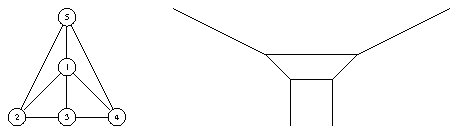
\includegraphics[width=0.66\textwidth]{figures/Fig_132_PDF238_Book226.pdf}
  \caption{例 8.17 的热带曲线与 Newton 多边形三角剖分（原书 p.226）}
  \label{fig:tropical-curve-genus-one}
\end{figure}
因此，对通有的 $t$，曲面 $\dot S=W_t^{-1}(0)\subset\mathbb C^{*2}$ 的亏格为 $1$，并有四个穿孔。
\end{example}

\section{一、二、三维镜像对称}\label{sec:one-two-three-mirror-symmetry}
\takeaway{同一个二维 Newton 多边形 $\square$ 可在复维 $1,2,3$ 中构造镜像：$A$ 侧依次是带穿孔黎曼曲面、Landau--Ginzburg 模型以及由 $UV=W_t$ 切出的三维超曲面；$B$ 侧是仿射环簇及其环簇除子，对应关系由矩阵分解、凝聚层与 wrapped/有向/正合 Fukaya 范畴的分裂导出等价给出。}
现在我们将研究镜像对称与环簇几何、热带几何之间的关系。出发点是 $n$ 维复环面上的一参数函数族
\[
  W_t\colon T^\vee\to\mathbb C,
\]
它使我们可以探索 $n-1,n,n+1$ 维中的镜像对称。为简单起见，假设 $\dim T^\vee=2$，于是得到一、二、三维中的对应关系。

\subsection{模型}\label{subsec:one-two-three-models}
我们先定义三个 $A$ 模型。每种情形中的辛几何都不依赖参数 $t$，因此可以令 $t\to\infty$，考察热带极限。于是 $A$ 模型只依赖于 Newton 多边形；当 $n=2$ 时，它是一个多边形。将其记为 $\square$，并用它作为以下三个 $A$ 模型的下标：
\begin{itemize}
  \item[(1D)] $Y^1_\square:=W_t^{-1}(0)$ 是对偶环面 $T^\vee=(\mathbb C^*)^2$ 中带穿孔的黎曼曲面。把穿孔附近补成柱形端后，它可视为一个 Liouville 子流形。
  \item[(2D)] $Y^2_\square:=(T^\vee,W_t)$ 是定义在复环面 $T^\vee\cong T^*(S^1)^2$ 上的 Landau--Ginzburg 模型，配备标准正合辛结构与体积形式。
  \item[(3D)]
  \[
    Y^3_\square:=\{(X,Y,U,V)\in T^\vee\times\mathbb C^2\mid
      UV=W_t(X,Y)\}
  \]
  是一个超曲面，可视为 $T^\vee\times\mathbb C^2=T^*(S^1)^2\times\mathbb R^2$ 中的正合辛子流形。也可以把它看作 $T^\vee$ 上的仿射圆锥截面族；当 $W_t=0$ 时，圆锥截面退化。
\end{itemize}
% [Tutor Note: 三个模型名字里的 1D、2D、3D 指复维数：$Y^1_\square$ 是黎曼曲面（实维 2），$Y^2_\square=(T^\vee,W_t)$ 是复曲面上的 Landau--Ginzburg 模型（实维 4），而 $Y^3_\square$ 是 $T^\vee\times\mathbb C^2$ 中由一个方程切出的超曲面，实维为 $4+4-2=6$。写镜像对应时不要混用复维与实维。]

由于 $W_t$ 是对偶环面 $T^\vee$ 上的函数，它的单项式指数属于 $N=\operatorname{Hom}(T^\vee,\mathbb C^*)$，所以 Newton 多边形是 $N_{\mathbb R}$ 的子集。在通有情形下取极限时，热带函数 $W_{\mathrm{trop}}$ 会在 Newton 多边形上诱导一个三角剖分，记作 $\boxtimes$。这个三角剖分将用于构造三个 $B$ 模型。

\begin{itemize}
  \item[(3D)] 把 Newton 多边形放在三维空间中的高度 $1$ 平面
  \[
    \square\times\{1\}\subset\mathbb R^3
  \]
  上，取它所张成的锥
  \[
    \sigma_\square=\mathbb R_{\geq0}(\square\times\{1\}).
  \]
  这确定一个三维仿射环簇
  \[
    X^3_\square=V(\mathbb C[\sigma_\square^\vee\cap M]).
  \]
  除非 $\square$ 是基本三角形（此时 $X^3_{\triangle}\cong\mathbb A^3$），否则该簇是奇异的。仿照例\ref{ex:ak-singularity-resolution}，把这个锥细分为覆盖三角剖分 $\boxtimes$ 中各基本三角形的小锥，即可消解奇点。这样得到光滑的三维环簇 $X^3_{\boxtimes}$ 和消解映射
  \[
    \pi\colon X^3_{\boxtimes}\to X^3_\square.
  \]
  这种消解称为 crepant 消解\index{crepantxiaojie@crepant 消解|hyperpage}。\footnote{消解 $\widetilde X\to X$ 称为 crepant 的，若 $X$ 上典范线丛的拉回等于 $\widetilde X$ 上的典范线丛。}
  % [Tutor Note: 环簇情形下“crepant”有一个纯组合的判据：细分所用的每条新射线都落在原锥的高度 $1$ 截面上（这里就是 $\square$ 的格点 $(a,b,1)$），于是细分不引入新的典范除子，$K_{X^3_\boxtimes}=\pi^*K_{X^3_\square}$。若射线来自更高层（如 $(a,b,2)$ 方向），消解就会多出未被消去的除子。]
  \begin{figure}[H]\centering
    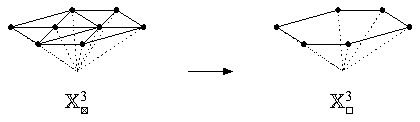
\includegraphics[width=0.73\textwidth]{figures/Fig_133_PDF240_Book228.pdf}
    \caption{三维仿射环簇及其消解（原书 p.228）}
    \label{fig:toric-threefold-crepant-resolution}
  \end{figure}
  \item[(2D)] $X^3_{\boxtimes}$ 的射线向量形如 $v=(a,b,1)$，其中 $(a,b)$ 是 Newton 多边形中的格点。令 $m=(0,0,1)$，则对所有射线向量 $v$ 都有 $\langle m,v\rangle=1$。这意味着函数
  \[
    \ell=X^m
  \]
  属于所有 $\mathcal O(U_\sigma)$，因此是一个整体函数。它的零点集是稠密环面的补集
  \[
    D=X^3_{\boxtimes}\setminus T,
  \]
  也就是所有环簇除子 $D_v$ 的并。每个环簇除子 $D_v$ 本身也是光滑环簇。其扇可如下构造：若射线向量 $v,w_1,w_2$ 构成 $\boxtimes$ 中的一个基本三角形，则
  \[
    \mathbb R_{\geq0}(w_1-v)+\mathbb R_{\geq0}(w_2-v)
  \]
  是平面 $\mathbb R^2\times\{0\}$ 中的一个锥。若 $v$ 是 $\square$ 的内部格点，该扇覆盖整个 $\mathbb R^2$，且 $D_v$ 位于消解映射 $\pi\colon X^3_{\boxtimes}\to X^3_\square$ 的零纤维中。我们把这个除子记为 $X^2_v$。
  \begin{figure}[H]\centering
    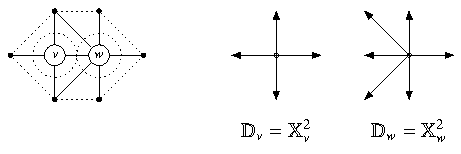
\includegraphics[width=0.55\textwidth]{figures/Fig_134_PDF240_Book228.pdf}
    \caption{环簇除子的局部扇（原书 p.228）}
    \label{fig:toric-divisor-fans}
  \end{figure}
  \item[(1D)] 最后考察 Landau--Ginzburg 模型
  \[
    X^1_{\boxtimes}:=(X^3_{\boxtimes},\ell).
  \]
  从 $B$ 模型的角度，它描述 $\ell$ 的零点集中的奇点；该奇点集是一维的。正如我们已经看到的，$\ell^{-1}(0)=X^2_{\boxtimes}$ 是若干光滑环簇除子的并，其奇点集就是这些除子的交。若 $D_v,D_w$ 的射线向量在扇中张成二维锥，那么这两个除子有一个公共的一维环面轨道（即 $\mathbb C^*$）。这恰好意味着三角剖分中的相应格点以一条边相连。若三个除子相交于一点，则其射线向量张成三维锥，也就是说相应三个格点构成三角剖分中的一个三角形。
\end{itemize}

因此，我们可以把具有同一三角剖分的热带曲线的几何与 $\ell^{-1}(0)$ 的奇点集联系起来。$\ell^{-1}(0)$ 的奇点集在热带曲线的每条边上有一个 $\mathbb C^*$，在每个顶点上有一个点。每条内部边连接两个顶点，相应的两个点与 $\mathbb C^*$ 合起来构成一个 $\mathbb P^1$；每条腿只连接一个顶点，所以相应的点与 $\mathbb C^*$ 合起来构成一个 $\mathbb A^1$。故奇点集是若干条射影直线与仿射直线组成的并，它们在三重交点处相接。
\begin{figure}[H]\centering
  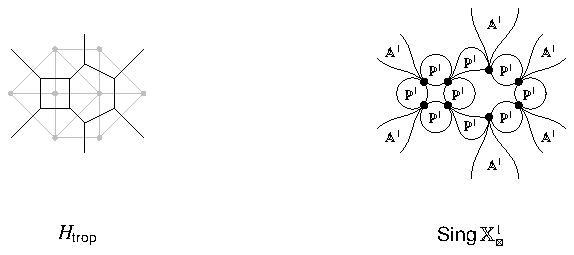
\includegraphics[width=0.92\textwidth]{figures/Fig_135_PDF241_Book229.pdf}
  \caption{热带曲线及 $X^1_{\boxtimes}$ 的奇点集（原书 p.229）}
  \label{fig:tropical-curve-singularity-locus}
\end{figure}

现在可以陈述三维中的镜像对应关系：
\begin{itemize}
  \item[(1D)] Landau--Ginzburg 模型 $X^1_{\boxtimes}$ 的矩阵分解范畴与带穿孔黎曼曲面 $Y^1_\square$ 的 wrapped Fukaya 范畴分裂导出等价：
  \[
    D^\pi\mathrm{MF}^{\pm}X^1_{\boxtimes}
    \simeq D^\pi\mathrm{wrFuk}^{\pm}Y^1_\square.
  \]
  \item[(2D)] 对 Newton 多边形中的每个内部格点 $v$，除子 $X^2_v$ 的凝聚层导出范畴嵌入 $Y^2_\square$ 这一 Landau--Ginzburg 模型的有向 Fukaya 范畴的分裂导出范畴：
  \[
    D\mathrm{Coh}^{\bullet}X^2_v
    \hookrightarrow D^\pi\mathrm{drFuk}^{\bullet}Y^2_\square.
  \]
  若 $X^2_v=\ell^{-1}(0)$，则这个嵌入是等价。
  \item[(3D)] 支撑在 $X^2_v$ 上的 $X^3_{\boxtimes}$ 凝聚层导出范畴嵌入 $Y^3_\square$ 的正合 Fukaya 范畴的分裂导出范畴：
  \[
    D\mathrm{Coh}^{\bullet}_{X^2_v}(X^3_{\boxtimes})
    \hookrightarrow D^\pi\mathrm{exFuk}^{\bullet}Y^3_\square.
  \]
\end{itemize}
构造这些等价有多种方法。下面简要说明每个维数中解决问题的思路。

\subsection{一维情形}\label{subsec:hms-dimension-one}
第一种方法是在两侧分别找出一组分裂生成元，再证明它们的 $A_\infty$ 自同态代数 $A_\infty$ 同构。一维情形的例子见\bookcite{1}。该文作者先考虑 Newton 多边形为基本三角形的情形。此时 $A$ 模型是三穿孔球面
\[
  Y^1_{\triangle}=\{(x,y)\in\mathbb C^{*2}\mid x+y+1=0\}
  \cong\mathbb C^*\setminus\{-1\},
\]
把穿孔补为柱形端后便是裤子曲面。$B$ 模型是 Landau--Ginzburg 模型
\[
  X^1_{\triangle}=(\mathbb A^3,XYZ),
\]
其奇点集由三条坐标轴组成。

$Y^1_{\triangle}$ 的 wrapped Fukaya 范畴有一组简单的锥形拉格朗日子流形 $L_x,L_y,L_z$，它们是分别连接两条柱形端的三条曲线。这些曲线把球面切成两个三角形，因此分裂生成 Fukaya 范畴。矩阵分解范畴也有三个简单的分裂生成元，它们对应于 $\mathbb A^3$ 中三条坐标轴的矩阵分解：
\[
  M_X=\left(R\underset{YZ}{\overset{X}{\rightleftarrows}}R\right),
  \quad M_Y=\left(R\underset{XZ}{\overset{Y}{\rightleftarrows}}R\right),
  \quad M_Z=\left(R\underset{XY}{\overset{Z}{\rightleftarrows}}R\right).
\]
\begin{figure}[H]\centering
  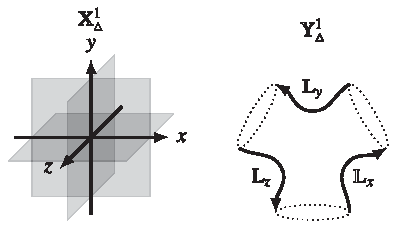
\includegraphics[width=0.92\textwidth]{figures/Fig_136_PDF242_Book230.pdf}
  \caption{裤子曲面上的三个生成曲线（原书 p.230）}
  \label{fig:pants-three-generators}
\end{figure}
\begin{figure}[H]\centering
  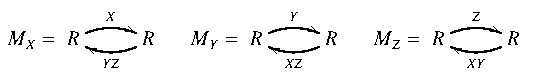
\includegraphics[width=0.88\textwidth]{figures/Fig_137_PDF242_Book230.pdf}
  \caption{三个坐标轴对应的矩阵分解（原书 p.230）}
  \label{fig:coordinate-axis-matrix-factorizations}
\end{figure}
可以计算出，两组生成元的 $A_\infty$ 自同态代数彼此 $A_\infty$ 同构，因此它们分裂生成的范畴等价。更多细节见第~\ref{sec:gentle-algebra-deformations}~节（参见定理~\ref{thm:gentle-ainfty-classification}）。

\begin{note}\label{note:pants-mirror-extensions}
\textbf{注 8.18.} Abouzaid 等人\bookcite{1}通过考察裤子曲面的覆盖，把这一技巧推广到更高亏格、带更多穿孔的黎曼曲面。在 $B$ 侧，这会得到一个带栈结构的 Landau--Ginzburg 模型；该模型也等价于一个拟射影模型。在文献\bookcite{36}中，同一技巧被用于构造非交换镜像，再利用箭图模空间将它们转化为拟射影模型。Pascaleff 与 Sibilla\bookcite{204}、Lee\bookcite{155}还发展了另一种方法：把三穿孔球面对应关系当作基本构件来处理其他情形。此时不寻找生成元，而是把多个三穿孔球面的 $A_\infty$ 范畴粘合起来。在 $A$ 侧，这种粘合可解释为把圆柱管缝在一起；在 $B$ 侧，则可看成把环境空间变为环簇。第\ref{ch:gluing}章将更详细地讨论这一点。最后，Nadler 与 Gammage\bookcite{190,94}提出的另一种粘合方法，把裤子曲面及其他带穿孔曲面的 Fukaya 范畴与微局部层理论联系起来。
\end{note}

\subsection{二维情形}\label{subsec:hms-dimension-two}
二维情形中的 $A$ 模型是一个 Landau--Ginzburg 模型。其对象是 $T^\vee$ 中边界落在 $W_t^{-1}(0)=Y^1_\square$ 上的拉格朗日圆盘。$Y^1_\square$ 在映射 $\log_t\colon T^\vee\to\mathbb R^2$ 下的像是 $W_t=\sum_{w\in\square}t^{a_w}Y^w$ 的阿米巴，是一块带若干孔的区域，这些孔记作 $(B_v)_t$。在通有情形下，每个孔对应 Newton 多边形中的一个格点 $v\in\square$。当 $t\to\infty$ 时，对应于 $v$ 的孔趋近多边形区域
\[
  \overline B_v=\{u\in\mathbb R^2\mid
  \text{对所有使 }[v,w]\text{ 成为 }\boxtimes\text{ 中一条边的 }w,
  \ \langle w-v,u\rangle+a_w-a_v\leq0\}.
\]
注意，向量 $w-v$ 正是 $X^2_v$ 的射线向量。为得到二维对应关系（更高维同理），Abouzaid\bookcite{5}比较了 $X^2_v$ 上的线丛与拉格朗日圆盘；当 $t\to\infty$ 时，这些圆盘经 $\log_t$ 映到 $(B_v)_t$ 上。

若 $X_\Delta$ 是环簇，且 $d\colon S_\Delta:=\Delta_1\to\mathbb Z$ 是从射线向量集合到整数的映射，则可在 $X_\Delta$ 上定义凝聚层 $\mathcal O(d)$：
\[
  \mathcal O(d)(U_\sigma)
  =\mathbb C\{X^m\mid\text{对所有 }v\in S_\Delta\cap\sigma,
    \ \langle v,m\rangle+d_v\geq0\}.
\]
从定义可见，$\mathcal O(0)=\mathcal O$ 是 $X_\Delta$ 的结构层；对每个 $d$，$\mathcal O(d)(U_\sigma)$ 都是有限生成的 $\mathcal O(U_\sigma)$-模。若 $X$ 光滑，则可证明对每个锥 $\sigma$，$\mathcal O(d)(U_\sigma)$ 都是秩一自由模，所以 $\mathcal O(d)$ 是线丛。其整体截面由多边形
\[
  P_d=\{m\in M_{\mathbb R}\mid
  \text{对所有 }v\in S_\Delta,\ \langle v,m\rangle+d_v\geq0\}
\]
中格点对应的单项式张成。
% [Tutor Note: 原文用 $S_\Delta$ 表示射线向量的集合，而前文（例 8.5 之后）把一维锥的集合记作 $\Delta_1$，二者应是同一个集合，属于记号不统一（见原书 p.231）。又 $\mathcal O(d)$ 的数据是每条射线上的整数 $d_v$，故 $d$ 的自由度就是射线数，在二维时等于 Newton 多边形的边数。]

若所有 $d_v$ 均为正，$P_d$ 与 $\overline B_v$“形状相同”（更准确地说，边的法向量方向相反）。因此存在一个光滑映射
\[
  \phi\colon\overline B_v\to P_d
\]
把角点对应起来，如下图所示。
\begin{figure}[H]\centering
  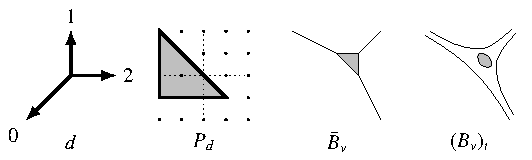
\includegraphics[width=0.86\textwidth]{figures/Fig_138_PDF244_Book232.pdf}
  \caption{线丛多边形与热带胞腔的对应（原书 p.232）}
  \label{fig:line-bundle-polytope-tropical-cell}
\end{figure}

把 $T^\vee$ 分解为
\[
  T^\vee\cong(S^1)^2\times\mathbb R^2=M_{\mathbb R}/M\times\mathbb R^2,
\]
并构造映射
\[
  \widetilde\phi\colon\overline B_v\to T^\vee,
  \qquad u\longmapsto(\phi(u)+M,u).
\]
它把 $\overline B_v$ 缠绕在实环面上，并且是 $\log_t|_{\overline B_v}$ 的截面。当 $t$ 足够大时，区域 $(B_v)_t$ 与 $\overline B_v$ 足够接近，可以微调这个映射，得到 $\log_t|_{(B_v)_t}$ 的一个拉格朗日截面 $L_d$，且它的边界落在 $W_t^{-1}(0)$ 上。这是 $Y^2_{\boxtimes}$ 的有向 Fukaya 范畴中的对象。

在特殊情形 $d=0$ 时，多边形 $P_d$ 是原点，$\phi$ 是常值映射；它提升为常值截面 $L_0$。$L_0$ 与 $L_d$ 的交点对应于 $P_d$ 中的格点，这正符合 $L_0,L_d$ 分别对应线丛 $\mathcal O(0),\mathcal O(d)$ 的预期。在文献\bookcite{5}中，Abouzaid 构造了 $X^2_{\boxtimes,v}$ 上的线丛预范畴到 $Y^2_{\boxtimes}$ 有向 Fukaya 预范畴中的嵌入。

对环簇而言，这些线丛分裂生成凝聚层的整个导出范畴\bookcite[命题 1.3]{5}。在 Fukaya 一侧，可以证明所有紧致 $(B_v)_t$ 上方的拉格朗日截面生成有向 Fukaya 范畴。因此，当内部格点只有一个时，该嵌入诱导导出等价。Abouzaid\bookcite{5}在所有维数中详细构造了这一过程。线丛预范畴与拉格朗日截面 Fukaya 范畴之间的等价，是通过一系列中间步骤建立的，其中使用了 $\overline B_v$ 上的 Morse 理论。

\begin{note}\label{note:del-pezzo-mirror}
\textbf{注 8.19.} del Pezzo 曲面（二维 Fano 簇）的情形也见于\bookcite{247}。Auroux、Katzarkov 与 Orlov\bookcite{11}采取了不同的方法，建立在 $k\leq8$ 个点处爆破的射影平面的导出范畴与 Landau--Ginzburg 模型 $W\colon M_k\to\mathbb C$ 的有向 Fukaya 范畴之间的联系。该方法目前只在二维中展开，但它适用范围更广，也包括非环簇 Fano 簇（$k\geq4$）。
\end{note}

\begin{note}\label{note:partially-wrapped-toric-mirror}
\textbf{注 8.20.} 也可以用 partially wrapped Fukaya 范畴描述 $A$ 模型。考虑实环面的余切丛 $T^*(S^1)^2$ 及投影
\[
  \pi\colon T^*(S^1)^2\to(S^1)^2,
\]
并取 $(S^1)^2$ 周围一个小管状邻域 $N_\epsilon$。多边形 $P_d$ 的每条边 $e$ 在实环面 $(S^1)^2=M_{\mathbb R}/M$ 中成为一个超平面。去掉 $N_\epsilon$ 后，该直线上方的余切纤维
\[
  F=\pi^{-1}(e)
\]
自然分成两部分：一部分协向量在指向 $P_d$ 外侧的切向量上取正值，另一部分取负值。分别记为 $E^+$ 和 $E^-$，并把所有 $E^+$ 的并作为 stop $\sigma$。partially wrapped Fukaya 范畴 $\mathrm{wrFuk}^{\bullet}_\sigma(T^*(S^1)^2)$ 与 $X^2_v$ 的导出范畴等价，因为对每个 $\mathcal O(d)$，可以重新缩放相应的 $\widetilde\phi$，使其落在 $N_\epsilon$ 内，并沿墙 $E^+\subset\sigma$ 继续上述嵌入。下图用一维多边形说明这一思路；此时余切丛是一个圆柱。
\begin{figure}[H]\centering
  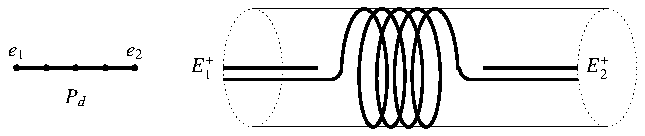
\includegraphics[width=0.90\textwidth]{figures/Fig_139_PDF245_Book233.pdf}
  \caption{一维截面上的 partially wrapped stop（原书 p.233）}
  \label{fig:partially-wrapped-stops-toric}
\end{figure}

这一方法与 Nadler、Zaslow\bookcite{195,187}提出的镜像对称中的可构造层与微局部层方法密切相关。对环簇，Bondal\bookcite{38}最先描述了可构造层方法，Fang 等人\bookcite{80,81}进一步发展。Morse 理论与微局部层之间的关系，参见 Ganatra、Pardon 与 Shende\bookcite{95}。
\end{note}

\subsection{三维情形}\label{subsec:hms-dimension-three}
为研究三维情形，需要考察环簇除子的嵌入
\[
  \iota\colon D_v=X^2_v\hookrightarrow X^3_{\boxtimes}.
\]
$X^2_v$ 上的每个线丛 $\mathcal O(d)$ 都可视为支撑在 $X^2_v$ 上的 $X^3_{\boxtimes}$ 上的层，因此是
\[
  \iota_*\mathcal O(d)\in D\mathrm{Coh}^{\bullet}_{X^2_v}(X^3_{\boxtimes})
\]
中的对象。要建立镜像对应，需要在 $Y^3_\square$ 中寻找一个以相同方式表现的对象。若计算 $D\mathrm{Coh}^{\bullet}_{X^2_v}(X^3_{\boxtimes})$ 中的自同态环，由 Serre 对偶性可知它具有 $\mathbb C\oplus\mathbb C[3]$ 的形式，这与三维球面的上同调同构。因此，一个自然想法是把拉格朗日截面 $L_d\in Y^2_\square$ 提升为 $Y^3_\square$ 中的拉格朗日球面。

前文已知，每个线丛 $\mathcal O(d)$ 对应于 $(B_v)_t$ 上方的一个拉格朗日截面 $L_d$。拓扑上，$L_d$ 是 $\mathbb C^{*2}$ 中的一张圆盘，边界落在 $W_t^{-1}(0)$ 上。三维空间 $Y^3_\square$ 可以看作 $\mathbb C^{*2}$ 上的圆锥曲线族
\[
  \{(u,v)\in\mathbb C^2\mid uv=W_t(x,y)\},
\]
而在 $W_t^{-1}(0)$ 上圆锥退化为锥。这个退化可以看作一个圆收缩为一点；所以在圆盘 $L_d$ 上方有一族圆，并在边界处收缩为点。该圆丛的全空间是一个三维球面。到目前为止我们只从拓扑角度定义了这个球面，但还可以把它实现为 $Y^3_\square$ 中的正合拉格朗日球面 $S_d$。对应关系
\[
  \iota_*\mathcal O(d)\longmapsto S_d
\]
延拓为全忠实嵌入
\[
  D\mathrm{Coh}^{\bullet}_{X^2_v}(X^3_{\boxtimes})
  \hookrightarrow D^\pi\mathrm{Fuk}^{\pm}Y^3_\square.
\]
\begin{figure}[H]\centering
  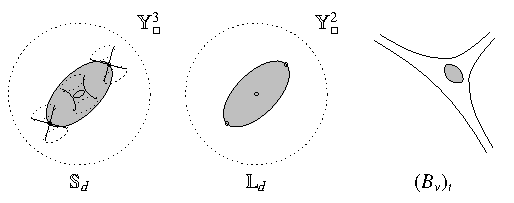
\includegraphics[width=0.73\textwidth]{figures/Fig_140_PDF246_Book234.pdf}
  \caption{三维镜像中球面与拉格朗日截面的关系（原书 p.234）}
  \label{fig:lagrangian-sphere-lift}
\end{figure}
Seidel\bookcite{219}详细研究了 Fano 情形；Abouzaid、Auroux 与 Katzarkov\bookcite{2}则将其推广到更一般的情形。

\section{远离大体积极限时}\label{sec:away-from-large-limit}
\takeaway{为得到紧流形，把曲线族紧化到环簇中并在每个柱形端放一个除子，得到 $\mathbb C[[q_1,\ldots,q_r]]$ 上的相对 Fukaya 范畴；$B$ 侧相应给势函数加入极端单项式，两侧参数由形式幂级数环的自同构联系。亏格 $2$ 曲线给出 Seidel 定理，椭圆曲线经极对偶给出反射多边形与 Batyrev 型构造。}
我们上面讨论的镜像对称例子都属于大体积极限。这里的意思是，辛形式测得的面积不起作用，因此可对 $\omega$ 重新缩放而不改变范畴。这也意味着可以在 $\mathbb C$ 上工作，而无须使用 Novikov 域。在 $B$ 侧，范畴只取决于环簇的组合结构。

大体积极限的缺点是，所考虑的辛流形必然非紧。若要研究紧辛流形，就必须通过添加额外结构来补全这些非紧版本。最直接的办法是加入除子，并考察相对 Fukaya 范畴。

先看曲线的情形。在大体积极限下，辛簇是带穿孔黎曼曲面 $Y^1_\square$，由 $W_t\colon\mathbb C^{*2}\to\mathbb C$ 的零点集确定。它是带柱形端的正合 Liouville 流形，每个穿孔对应一个端，也等价于热带曲线的一条无限腿。每条腿由 $W_t$ 的 Newton 多边形边界上的一条基本边确定。最容易想象的例子是三穿孔球面：把
\[
  X+Y+1=0\subset\mathbb C^{*2}
\]
嵌入射影平面，即可将它紧化为射影直线。
\begin{figure}[H]\centering
  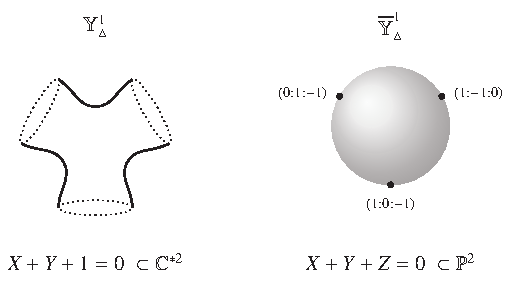
\includegraphics[width=0.64\textwidth]{figures/Fig_141_PDF247_Book235.pdf}
  \caption{三穿孔球面的射影紧化（原书 p.235）}
  \label{fig:pants-projective-compactification}
\end{figure}
一般的 $Y^1_\square$ 如何紧化？思路是把 $\mathbb C^{*2}$ 紧化为环簇 $V$，再考察 $Y^1_\square\subset\mathbb C^{*2}\subset V$ 的闭包。函数 $W_t$ 是若干单项式的线性组合，这些单项式对应 Newton 多边形 $\square$ 中的格点。我们可以把它们解释为环簇上某个线丛 $\mathcal O(d)$ 的截面；该簇的射线向量是 Newton 多边形各边的向内法向量。这个簇或其某个适当的消解，就是所需的紧化。

\begin{example}[两种环簇紧化]\label{ex:toric-compactifications}
考察以下两个例子。
\begin{enumerate}[label=(\roman*)]
  \item\label{ex:triangle-compactification} 令
  \[
    W_t=t+X+Y+X^{-1}Y^{-1}.
  \]
  其 Newton 多边形是由
  \[
    m_1=(1,0),\qquad m_2=(0,1),\qquad m_3=(-1,-1)
  \]
  张成的三角形，各边的向内法向量为
  \[
    n_1=(2,-1),\qquad n_2=(-1,2),\qquad n_3=(-1,-1).
  \]
  构造二维锥为 $\mathbb R_{\geq0}n_i+\mathbb R_{\geq0}n_j$ 的环簇 $V$。这个簇不是光滑的，但对其锥作细分可以得到消解 $\widetilde V$；补集 $\widetilde V\setminus\mathbb C^{*2}$ 由九条 $\mathbb P^1$ 组成，每条对应一条射线向量，并且这些射影直线按环状相交。
  \begin{figure}[H]\centering
    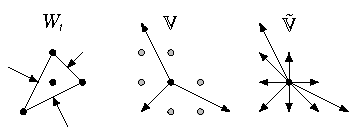
\includegraphics[width=0.48\textwidth]{figures/Fig_142_PDF247_Book235.pdf}
    \caption{三角形 Newton 多边形及其环簇消解（原书 p.235）}
    \label{fig:triangle-toric-compactification}
  \end{figure}
  函数 $W_t$ 可视为 $\mathcal O_V(1)$ 的截面，其中 $1$ 把每个射线向量 $n_i$ 映到 $1$；它也可视为 $\mathcal O_{\widetilde V}(1)$ 的截面。对通有的 $W_t$，零点集 $\overline Y^1_\square$ 与对应于 $n_i$ 的三条 $\mathbb P^1$ 各交于一点 $p_i$，但不与另外六条新增的 $\mathbb P^1$ 相交。
  \item\label{ex:projective-plane-compactification} 令
  \[
    W_t=t+X^2Y^{-1}+XY^{-1}+Y^{-1}+X^{-1}Y^{-1}
        +X^{-1}+X^{-1}Y+X^{-1}Y^2+Y+X.
  \]
  此时 Newton 多边形的三个法向方向为
  \[
    n_1=(1,0),\qquad n_2=(0,1),\qquad n_3=(-1,-1),
  \]
  相应的环簇就是光滑的 $\mathbb P^2$。该曲面有三条 $\mathbb P^1$；因为相应的方程是三次方程（等价地，热带曲线沿每条边有三条腿），$W_t^{-1}(0)$ 的紧化与每条 $\mathbb P^1$ 都交于三点。
  \begin{figure}[H]\centering
    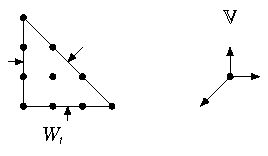
\includegraphics[width=0.53\textwidth]{figures/Fig_143_PDF248_Book236.pdf}
    \caption{第二个 Newton 多边形紧化示意（原书 p.236）}
    \label{fig:second-toric-compactification}
  \end{figure}
\end{enumerate}
\end{example}

我们可以通过加入一个除子 $D$ 来形变 wrapped Fukaya 范畴，其中 $D$ 在每个柱形端各取一点。但如例 8.21(ii) 所示，有些柱形端在紧化后会落在同一个除子上。这提示我们应给这些端使用相同的形变系数，从而得到定义在
\[
  \mathbb C[[q_1,\ldots,q_r]]
\]
上的相对 Fukaya 范畴 $\mathrm{cuFuk}^{\pm}(Y^1_\square,D)$，其中 $r$ 是 Newton 多边形边的数目。

要得到镜像对应，还需要形变 $B$ 模型。回忆一下，带穿孔黎曼曲面的镜像是 Landau--Ginzburg 模型 $(X^3_\square,\ell)$，其中整体函数 $\ell$ 是 $X^m\in\mathcal O(X^3_\square)$，且 $m=(0,0,1)\in M$。对这个 $B$ 模型，最简单的形变方法是给 $\ell$ 添加单项式项。它们必须来自结构层的整体截面：
\[
  \mathcal O(X^3_\square)
  =\mathbb C\{X^m\mid
  \text{对所有 }u\in\square,\ \langle m,(u,1)\rangle\geq0\}.
\]
这些单项式对应于对偶锥 $\sigma^\vee_\square$ 中的格点。该锥的射线向量与 $\sigma_\square$ 的面互为对偶，而这些面又与 $\square$ 的边一一对应。因此，对偶锥由形如
\[
  e_i=(n_i,c_i)
\]
的向量张成，其中 $n_i$ 是 $\square$ 某条边的向内法向量，$c_i\in\mathbb Z$ 则取决于 $\square$ 在 $\mathbb R^2$ 中的位置。这些射线向量对应的单项式称为极端单项式，可以加入势函数。首先考察 Landau--Ginzburg 模型
\[
  \mathrm{cuTw}(X^3_\square,\ell_q),
  \qquad \ell_q=\ell+\sum_iq_iX^{e_i}.
\]
这给出定义在 $\mathbb C[[q_1,\ldots,q_r]]$ 上的带曲率范畴，其中 $r$ 是多边形的边数。它恰好等于 $A$ 模型形变所用的参数数目。因此，我们预期这两种形变彼此对应，并由此在无曲率部分之间得到导出等价。当然，不能指望两侧的参数空间直接一一对应；我们预期存在形式幂级数环的一个自同构 $\alpha$，把两侧的参数互相转换。
\begin{figure}[H]\centering
  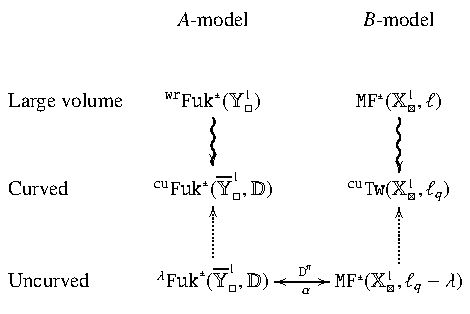
\includegraphics[width=0.82\textwidth]{figures/Fig_144_PDF249_Book237.pdf}
  \caption{$A$、$B$ 模型中的大体积极限与曲率形变（原书 p.237）}
  \label{fig:large-volume-curved-models}
\end{figure}

若在 $\overline Y^1_\square$ 上选择特定的辛形式 $\omega$，则可在 $A$ 侧对 Novikov 环上的完整 Fukaya 范畴工作。此时我们预期存在一个环同态
\[
  \beta\colon\mathbb C[[q_1,\ldots,q_r]]\to\Lambda
\]
实现参数之间的转换。这些启发式想法已在若干具体情形中得到部分验证。

\subsection*{亏格为 2 的曲线}
取环 $\mathbb C[X,Y,Z]$，并令群 $G=\langle g\mid g^5=1\rangle$ 作用为
\[
  g(x,y,z)=(\zeta x,\zeta y,\zeta^3z),
\]
其中 $\zeta$ 是五次单位根。为了求不变量，先考察 $\mathbb C[X^{\pm1},Y^{\pm1},Z^{\pm1}]^G$。此环由
\[
  U=XY^{-1},\qquad V=X^2Y^3,\qquad W=XYZ
\]
自由生成，并且
\[
  U^iV^jW^k\in\mathbb C[X,Y,Z]
  \quad\Longleftrightarrow\quad
  i+2j+k\geq0,\quad -i+3j+k\geq0,\quad k\geq0.
\]
因此，不变量环同构于由锥
\[
  \sigma=\mathbb R_{\geq0}(1,2,1)
       +\mathbb R_{\geq0}(-1,3,1)
       +\mathbb R_{\geq0}(0,0,1)
\]
张成的仿射环簇。由此
\[
  \mathbb A^3//G\cong X^3_\square,
\]
其中 $\square$ 如下图所示。
\begin{figure}[H]\centering
  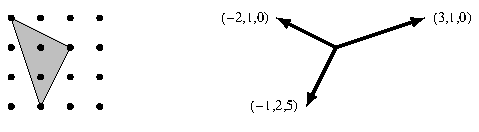
\includegraphics[width=0.62\textwidth]{figures/Fig_145_PDF249_Book237.pdf}
  \caption{亏格 2 曲线对应的 Newton 多边形（原书 p.237）}
  \label{fig:genus-two-newton-polygon}
\end{figure}

这与 Newton 多边形顶点为 $(1,2),(-1,3),(0,0)$ 的 $X^3_\square$ 相同。固定该多边形的任一三角剖分，都可以把 $X^3_{\boxtimes}$ 解释为 $\mathbb A^3//G$ 的一个消解。另一方面，$A$ 模型 $Y^1_\square$ 是一条亏格为 $2$、带三个穿孔的曲线，因为这个多边形有两个内部格点、三个边界格点。

在 $A$ 侧填上穿孔，对应于按照对偶锥的射线加入单项式：
\[
  U^3V=X^5,\qquad U^{-2}V=Y^5,\qquad
  U^{-1}V^{-2}W^5=Z^5.
\]
因此可以把势函数写为不变函数
\[
  \ell_q=XYZ+q_1X^5+q_2Y^5+q_3Z^5.
\]
在 $A$ 侧和 $B$ 侧，参数都没有出现在无穷级数中，所以镜像对应可以用普通的 $\mathbb C$-线性范畴表述。

\begin{theorem}{Seidel 的亏格二镜像定理\bookcite{220}}{seidel-genus-two-mirror}
设 $\Sigma_2$ 是一条亏格为 $2$ 的曲线，将其视为辛流形，并令 $\widetilde X$ 是 $\mathbb A^3//\mathbb Z_5$ 的一个 crepant 消解\index{crepantxiaojie@crepant 消解|hyperpage}，则有等价
\[
  D^\pi\mathrm{Fuk}^{\pm}(\Sigma_2)
  \cong_\infty D^\pi\mathrm{MF}^{\pm}
  (\widetilde X,XYZ-X^5-Y^5-Z^5).
\]
\end{theorem}
\begin{proof}[证明思路]
该定理由构造一个生成元并证明其自同态环是外代数 $\Lambda_3$ 的形变，再通过分类外代数的形变来证明这些形变彼此等价。也可以不用 $\widetilde X$，而直接在商栈 $[\mathbb A^3/\mathbb Z_5]$ 上工作。更多内容见\bookcite{220}。
\end{proof}

\begin{note}\label{note:efimov-higher-genus}
\textbf{注 8.23.} Efimov\bookcite{71}利用 $\mathbb Z_{2g+1}$ 在 $\mathbb A^3$ 上的作用，把该定理推广到了亏格 $g\geq3$ 的曲线。
\end{note}

\subsection*{椭圆曲线}
对椭圆曲线可以采取类似策略，考察 $\mathbb A^3$ 上的 $\mathbb Z_3$ 作用；此时会出现一些额外特征。首先，椭圆曲线是 Calabi--Yau 流形，因此可以把 Fukaya 范畴提升为 $\mathbb Z$-分次版本。另一方面，多项式 $\ell_q$ 是三次齐次的，所以可以考察分次矩阵分解，而非普通矩阵分解。Orlov 的结果使我们能够把分次矩阵分解范畴
\[
  \mathrm{grMF}^{\bullet}(\mathbb C[X,Y,Z],\ell_q)
\]
解释为 $\mathbb P^2$ 中 $\ell_q$ 零点集的凝聚层导出范畴；该零点集又是一条椭圆曲线 $E^\vee$。因此预期有对应
\[
  D^\pi\mathrm{Fuk}^{\bullet}(E,D)
  \cong_\infty\mathrm{grMF}^{\bullet}(\mathbb C[X,Y,Z],\ell_q)
  \cong_\infty D\mathrm{Coh}^{\bullet}E^\vee.
\]
与高亏格曲线的情形不同，$A$ 侧有无穷多个圆盘，所以形变参数会出现幂级数。

椭圆曲线的镜像仍是椭圆曲线，这一点已在许多框架下得到详细研究。Polishchuk 与 Zaslow\bookcite{205}最先描述了凝聚层导出范畴对象与 Fukaya 范畴对象之间的对应。Lekili 与 Perutz\bookcite{162,161}研究了单个除子的相对 Fukaya 范畴情形；Lekili 与 Polishchuk\bookcite{164}研究了由多个点组成的除子情形。他们从椭圆曲线的另一种表示出发。关于 $E^\vee\subset\mathbb P^2$ 及其非交换推广，参见 Cho、Hong 与 Lau 的工作\bookcite{55,154}。

\subsection*{极对偶性\index{jiduiou@极对偶|hyperpage}}
椭圆曲线的 $A$、$B$ 模型之间还存在一种引人注目的对称性。由例\ref{ex:toric-compactifications}可知，椭圆曲线 $E=Y^1_\square$ 就是例 8.21\hyperref[ex:triangle-compactification]{(i)}的紧化 $\widetilde V$ 中 $W_t$ 的零点集；而 $E^\vee$ 是 $\ell_q$ 在 $\mathbb P^2$ 中的零点集，$\mathbb P^2$ 正是该例\hyperref[ex:projective-plane-compactification]{(ii)}所用的紧化。因此，$W_t$ 与 $\ell_q$ 都在由含一个内部格点的多边形所对应的环簇中切出一条椭圆曲线。

\begin{definition}{反射多边形与极对偶多边形}{reflexive-polygon}
若 Newton 多边形 $\square$\index{fansheduobianxing@反射多边形|hyperpage} 恰有一个内部格点，且该点为 $0\in\mathbb Z^2=M$，则称 $\square$ 为反射多边形。这意味着 $\square$ 的边可写为
\[
  \langle m,u\rangle+1=0,
\]
其中 $u$ 是 $\operatorname{Hom}(M,\mathbb Z)=M^\vee=N$ 中的本原向量。由这些向量张成的凸包 $\diamond\subset N_{\mathbb R}$ 称为极对偶多边形。注意，由 $u$ 与 $m$ 的对称性可知，极对偶多边形 $\diamond$ 也仍是反射多边形。
\end{definition}

\begin{theorem}{二维反射多边形分类}{classification-reflexive-polygons}
在 $\mathrm{GL}_2(\mathbb Z)$ 变换意义下，恰有 $16$ 个反射多边形，如下图所列。其中前六列两两构成对偶对，最后两列则在某个线性变换下自对偶。
\begin{figure}[H]\centering
  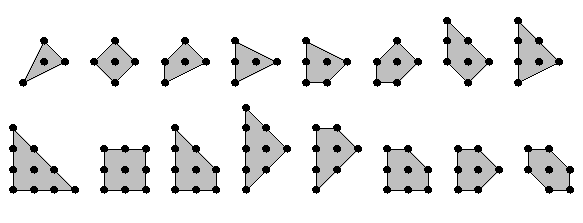
\includegraphics[width=0.82\textwidth]{figures/Fig_146_PDF251_Book239.pdf}
  \caption{二维反射多边形及其极对偶关系（原书 p.239）}
  \label{fig:sixteen-reflexive-polygons}
\end{figure}
\end{theorem}

从一个反射多边形 $\square$ 出发，把 $v=(0,0)$ 与其顶点相连，就得到一个奇异 Fano 簇的扇；再把 $v$ 连到边界上的其他格点即可消解其奇点。所得消解 $V=X^2_v$ 是弱 Fano 簇，这是 Fano 簇的轻微推广。线丛 $\mathcal O_V(1)$ 的整体截面是由极对偶多边形 $\diamond$ 中的单项式线性组合而成。取通有整体截面 $W\in\mathcal O_V(1)(V)$，其零点集是一条椭圆曲线 $E\subset V$，即一维 Calabi--Yau 簇。对极对偶多边形作同样构造，得到另一个弱 Fano 簇 $V^\vee$ 及其截面 $W^\vee$；后者的零点集是另一条椭圆曲线 $E^\vee\subset V^\vee$。对于适当的辛结构和整体截面选择，我们预期 $E$ 的 Fukaya 范畴与 $E^\vee$ 的凝聚层导出范畴等价，反向亦然。若 $\square$ 是图中第一种反射多边形，就得到上一小节描述的对应；若是第二种，则得到嵌入 $\mathbb P^1\times\mathbb P^1$ 的椭圆曲线镜像对称，详见\bookcite{154}。

这一总体思想最早由 Batyrev\bookcite{22}提出。每个 $n$ 维反射多面体都定义一个带线丛的 $n$ 维弱 Fano 簇。该线丛的通有截面给出一个 Calabi--Yau 超曲面；镜像 Calabi--Yau 簇则由极对偶多面体按同样方式构造。
% [Tutor Note: 极对偶的几何内容是“交换 Kähler 自由度与复结构自由度”：$\square$ 一侧给出弱 Fano 簇 $V$ 上的椭圆曲线 $E$，$\diamond$ 一侧给出 $V^\vee$ 上的 $E^\vee$，而 $W$ 与 $W^\vee$ 的系数分别充当对方的模参数。二维反射多边形恰有 $16$ 个，对应 $16$ 类 del Pezzo 型弱 Fano 曲面；这是 Batyrev 对偶在复二维的实例。]

这一设想已从许多角度得到研究并向多个方向推广\bookcite{24,25}。在经典镜像对称方法中，它被用于验证若干重要镜像对的 Hodge 数猜想\bookcite{22,23,56}。从同调镜像对称角度看，Seidel\bookcite{221}研究了 $\mathbb P^3$ 中的四次超曲面情形（相应反射多面体由 $\mathbb R^3$ 的标准坐标向量与 $(-1,-1,-1)$ 张成）。再高一维，$\mathbb P^4$ 中的五次超曲面是最初引出镜像对称的例子\bookcite{51}。这一情形的同调版本由 Nohara 与 Ueda\bookcite{194}证明，更一般的各维情形由 Sheridan\bookcite{223}证明。

\subsection*{Landau--Ginzburg 模型之间的镜像对称}
我们不一定只能得到两个 Calabi--Yau 簇之间的对应；也可以推广这一构造，得到两个 Landau--Ginzburg 模型之间的镜像对称。设 $a=(a_{ij})$ 是一个系数为正整数的可逆 $n\times n$ 矩阵。由 $a$ 构造多项式
\[
  W_a=\sum_iX_1^{a_{i1}}\cdots X_n^{a_{in}}
\]
和环 $R=\mathbb C[X_1,\ldots,X_n]$。$W_a$ 中的每个单项式都是环面 $T\subset\mathbb A^n=V(R)$ 上的特征。在 $T$ 中有一个固定 $W_a$ 的有限子群 $G_a$，我们取定其子群 $\Gamma\subset G_a\subset T$。

对偶一侧的多项式环为 $R^\vee=\mathbb C[Y_1,\ldots,Y_n]$，对偶多项式为
\[
  W_a^\vee=\sum_iY_1^{a_{1i}}\cdots Y_n^{a_{ni}}.
\]
固定 $W_a^\vee$ 的有限子群 $G_a^\vee$ 可自然认作 $\operatorname{Grp}(G_a,\mathbb C^*)$，并把 $\Gamma$ 的湮灭子群记作 $\Gamma^\vee$。由此得到两个带栈结构的 Landau--Ginzburg 模型
\[
  ([\mathbb A_X^n/\Gamma],W_a),
  \qquad ([\mathbb A_Y^n/\Gamma^\vee],W_a^\vee),
\]
它们应当互为镜像。与前述情形类似，一侧势函数中的每个单项式对应于另一侧仿射空间中的一个环簇除子；现在还包含额外的 orbifold 群作用，用以记录这些单项式可能是射线向量的倍数这一事实。

最简单的情形是 $n=1$ 且 $\Gamma$ 平凡；此时 $W_a=X^a$、$W_a^\vee=Y^a$，并且
\[
  D^\pi\mathrm{drFuk}^{\pm}(\mathbb C,X^a)
  \cong_\infty\mathrm{MF}^{\pm}(\mathbb C[Y]\star\mathbb Z_a,Y^a).
\]
左侧可以重新解释为 $\mathbb C$ 上带有趋向无穷远 stop 的 partially wrapped Fukaya 范畴；等价地，是边界上标有 $a$ 个点的圆盘的 Fukaya 范畴。从这个角度看，我们重新得到与第\ref{subsec:linear-quiver}节线性箭图相应的镜像对称。

这套思想也可用于尖点奇点 $(\mathbb A^2,X^3+Y^2)$ 的镜像对称（见\bookcite{161}，更一般情形见\bookcite{107}）；Ueda\bookcite{247}、Lekili\bookcite{169}等人也研究了相关对偶。此外，这些带栈结构的模型还可以与任意环簇结合使用\bookcite{59}。

\section{镜像与纤维化}\label{sec:mirrors-and-fibrations}
\takeaway{SYZ 猜想断言镜像对由互为对偶的特殊拉格朗日环面纤维化联系：$X^\vee$ 上的点层对应 $X$ 中带 $U(1)$ 局部系统的拉格朗日环面，故 $X^\vee$ 是这些环面的模空间。大体积极限下由矩映射 $\log_t$ 实现该纤维化，并由 Gross--Siebert 退化给出组合版本。}
我们已经看到，利用热带几何与环簇几何之间的对偶，可以寻找镜像对并证明一些同调镜像对称实例。从历史上看，这种解释出现得较晚。镜像对称最初只针对紧致 Calabi--Yau 流形提出，涉及计数伪全纯映射的数值不变量与镜像流形上的某些复积分之间的对偶。这些不变量的关系最初表述为生成函数之间的对应，后来才被重新解释为范畴等价。

为了描述两个镜像流形之间的关系，Strominger、Yau 与 Zaslow\bookcite{237}借助弦论中的 $T$-对偶提出一个猜想，下面将予以讨论。$T$-对偶的若干数学处理可参见\bookcite{19,77}。

\subsection{SYZ 纤维化}\label{subsec:syz-fibrations}
回忆一下，$n$ 维 Calabi--Yau Kähler 流形 $M$ 带有三种结构：复结构
\[
  J\colon TM\to TM,
\]
辛结构 $\omega\in\Omega^2M$，与复体积形式 $\Omega\in\Omega^n_{\mathbb C}M$。

\begin{definition}{特殊拉格朗日子流形与特殊拉格朗日环面纤维化}{special-lagrangian-fibration}
若拉格朗日子流形 $L\subset M$ 上的复体积形式 $e^{-i\theta}\Omega$ 限制为实体积形式，则称 $L$ 为相位 $\theta$ 的特殊拉格朗日子流形\index{teshulagelangriziliuxing@特殊拉格朗日子流形|hyperpage}。若映射 $\pi\colon M\to B$ 的每个纤维都是具有相同相位的特殊拉格朗日环面，则称 $\pi$ 为特殊拉格朗日环面纤维化\index{teshulagelangrihuanmianxianweihua@特殊拉格朗日环面纤维化|hyperpage}。
\end{definition}

\begin{example}[椭圆曲线的特殊拉格朗日纤维化]
考虑复流形
\[
  M=\mathbb C/(\mathbb Z+i\mathbb Z),
\]
配备辛形式 $\omega=dx\wedge dy$，其中 $z=x+iy$ 是 $\mathbb C$ 上的标准坐标。取复体积形式 $\Omega=dz$。这个一维紧致 Calabi--Yau 流形有一个显然的特殊拉格朗日环面纤维化，其底空间为 $B=\mathbb R/\mathbb Z$：
\[
  \pi\colon M\to B,\qquad x+iy\longmapsto y.
\]
该映射的纤维是水平圆周，所以纤维化的相位为 $0$。若改为投影到 $x$ 坐标，则得到相位为 $\pi/2$ 的纤维化。更一般地，对每个
\[
  A=\begin{pmatrix}a&c\\b&d\end{pmatrix}\in\mathrm{GL}(2,\mathbb Z),
\]
映射 $\pi\circ A^{-1}$ 都给出一个相位为 $\arg(a+bi)$ 的特殊拉格朗日环面纤维化。
\end{example}

还可以用另一种方式看这个例子。考察圆周 $S^1$ 及其余切丛 $T^*S^1$。该余切丛是平凡向量丛，因此可以在每个纤维 $T_p^*S^1$ 中选取一个格 $\Lambda_p^*\subset T_p^*S^1$。余切丛有自然辛结构，该结构自然下降到商丛
\[
  M=T^*S^1/\Lambda^*.
\]
特殊拉格朗日子流形恰好是纤维
\[
  L_p=T_p^*S^1/\Lambda_p^*.
\]
另一方面，切丛 $TS^1$ 带有自然复结构，而格 $\Lambda_p^*\subset T_p^*S^1$ 确定一个对偶格 $\Lambda_p\subset T_pS^1$。向量空间 $V$ 中一个格的对偶格由所有把该格映到 $\mathbb Z$ 的协向量组成。若该格有一组基，则其对偶格由对偶基生成。对偶格取商便得到实环面
\[
  M^\vee=TS^1/\Lambda,
\]
和配对
\[
  \langle\ ,\ \rangle_p\colon
  T_p^*S^1/\Lambda_p^*\times T_pS^1/\Lambda_p
  \longrightarrow\mathbb R/\mathbb Z\cong U(1).
\]
整体上，这给出如下图表，其中纤维两两对偶：
\begin{figure}[H]\centering
  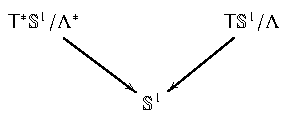
\includegraphics[width=0.43\textwidth]{figures/Fig_147_PDF255_Book243.pdf}
  \caption{余切环面与切环面的对偶纤维（原书 p.243）}
  \label{fig:cotangent-torus-duality}
\end{figure}
\begin{figure}[H]\centering
  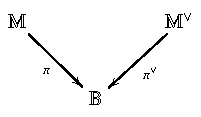
\includegraphics[width=0.38\textwidth]{figures/Fig_148_PDF255_Book243.pdf}
  \caption{两对偶环面纤维化在共同底空间上的对应（原书 p.243）}
  \label{fig:dual-torus-fibrations}
\end{figure}

由于 $M$ 与 $M^\vee$ 构成镜像对，这提示镜像流形应当由互为对偶的拉格朗日纤维化联系起来。一般而言，紧致 Calabi--Yau 流形上的特殊拉格朗日环面纤维化很难找到\bookcite{102,101,103}；多数情形下，除非放宽对 $\pi$ 的要求，否则它们并不存在。首先，不应要求底空间 $B$ 是光滑流形；其次，也不应要求每个纤维都是特殊拉格朗日环面，只要求通有纤维如此\bookcite{129}。也就是说，只有在 $B$ 的一个稠密开子集上，纤维才是互为对偶的特殊拉格朗日环面。特殊拉格朗日纤维化的背景可参阅 Hitchin\bookcite{113} 与 Joyce\bookcite{128} 的讲义。

\begin{conjecture}{Strominger--Yau--Zaslow\bookcite{237}}{syz-conjecture}
若两个 Calabi--Yau 流形 $(M,M^\vee)$ 互为镜像，则存在一个底空间 $B$ 及映射 $\pi,\pi^\vee$，使图表
\[
\begin{array}{ccc}
  M & \xrightarrow{\,\pi\,} & B \\[-2pt]
  M^\vee & \xrightarrow{\,\pi^\vee\,} & B
\end{array}
\]
所表示的 $\pi\colon M\to B$ 与 $\pi^\vee\colon M^\vee\to B$ 都是（可能奇异的）特殊拉格朗日环面纤维化；并且对一般点 $b\in B$，存在配对
\[
  \langle\ ,\ \rangle_b\colon
  \pi^{-1}(b)\times(\pi^\vee)^{-1}(b)\to U(1).
\]
\end{conjecture}

这个猜想与同调镜像对称有何关系？回忆一下，完整 Fukaya 范畴中我们关注的对象是带 $U(1)$ 局部系统的拉格朗日子流形（见注~\ref{note:unitary-local-systems}）。若 $X$ 与 $X^\vee$ 互为镜像，则有等价
\[
  D^\pi\mathrm{Fuk}(X)\cong D^\pi\mathrm{Coh}(X^\vee).
\]
$X^\vee$ 上的点层是 $D^\pi\mathrm{Coh}(X^\vee)$ 中的对象，其自同态代数是外代数。粗略来说，拉格朗日子流形 $L$ 的自同态代数等于它的上同调环；因此我们预期，点层会对应于带局部 $U(1)$-系统的拉格朗日环面。

这表明，一般而言，$X^\vee$ 上点层的模空间应当参数化 $X$ 上带 $U(1)$-局部系统的平行拉格朗日环面。对每个拉格朗日环面，可选的 $U(1)$-局部系统本身构成一个实 $n$ 维环面。因此，$X^\vee$ 一般由若干个实 $n$ 维环面组成；同一个拉格朗日环面对应的点层位于同一个这样的环面中。把这些环面取商，便得到某个 $n$ 维空间 $B$ 及映射 $\pi^\vee\colon X^\vee\to B$。

位于不同点的两个点层之间没有态射，这类似于两个不相交拉格朗日子流形之间的 Hom 空间为零。这提示 $B$ 中不同点对应的拉格朗日环面彼此不相交；这族 $n$ 维环面一般会铺满 $2n$ 维空间 $X$，从而得到投影 $\pi\colon X\to B$。纤维
\[
  L_b=\pi^{-1}(b)
\]
是一个环面，可写作 $\mathbb R^n/\Lambda$，其中格 $\Lambda\cong\pi_1(L_b)$。$L_b$ 上的 $U(1)$ 局部系统空间自然同构于对偶环面：
\[
  \operatorname{Hom}(\Lambda,U(1))
  \cong\operatorname{Hom}(\Lambda,\mathbb R/\mathbb Z)
  \cong\frac{\operatorname{Hom}(\Lambda,\mathbb R)}
  {\operatorname{Hom}(\Lambda,\mathbb Z)}
  \cong\frac{\mathbb R^n}{\Lambda^*}.
\]
% [Tutor Note: 第二处同构用了 $\Lambda\cong\mathbb Z^n$：逐个生成元提升即可看出 $\operatorname{Hom}(\Lambda,\mathbb R)\to\operatorname{Hom}(\Lambda,\mathbb R/\mathbb Z)$ 满射，其核正是 $\operatorname{Hom}(\Lambda,\mathbb Z)$。最后一步把 $\Lambda$ 换成对偶格 $\Lambda^*=\operatorname{Hom}(\Lambda,\mathbb Z)$；若改变 $\Lambda$ 与 $\pi_1(L_b)$ 的同一化，$B$ 的坐标会差一个 $\mathrm{GL}(n,\mathbb Z)$ 变换，这正是镜像构造中的整变换不确定性。]
这番推理并非证明，却说明了在一定条件下 SYZ 猜想成立的缘由。另一种观点见\bookcite{245}。

SYZ 猜想为镜像对的存在提供了漂亮的几何解释，但它既不容易证明，也不清楚是否在完全一般的情形下成立\bookcite{130}。一个原因是，特殊拉格朗日子流形通常很难构造，更不用说构造几乎覆盖整个空间的一族此类子流形。此外，纤维化的底空间通常是奇异的；如何构造这个底空间、它应满足哪些性质，都还不清楚。

\subsection*{极限情形}
为绕开这些困难，最好考察大体积极限等极限情形。此时可以利用环簇几何与热带几何之间的对偶。复环面有一个自然的拉格朗日环面纤维化
\[
  \log_t\colon T\to\mathbb R^n.
\]
若 $V$ 是一个环簇，其射线向量垂直于多面体 $\square$ 的各边，则可用矩映射 $\mu\colon V\to\square$ 延拓这个纤维化，使 $T$ 映到 $\square$ 的内部，而每个射线向量对应的除子映到相应的面\bookcite{89}。

现在设
\[
  W_t=1+tf,
\]
其中 $f$ 是 Newton 多面体为反射多面体 $\square$ 的通有函数。纤维 $W_t^{-1}(0)\subset\mathbb C^{*n}$ 可紧化为一族 $\overline Y_t\subset V$。当 $t\ne0$ 时，映射 $\mu|_{\overline Y_t}$ 不是拉格朗日环面纤维化；但在极限 $t\to0$ 时，它变为这样的纤维化，此时族退化为
\[
  \overline Y_0=\widetilde V\setminus\mathbb C^{*n},
\]
即若干环簇的并。每个多边形的面对应一个环簇；两个面相交时，对应的环簇也相交。另一方面，极对偶多边形给出第二族 $\overline Y^\vee_t$，可视为第一族的镜像。其极限同样是若干环簇的并，但由于极对偶性，它的交复形与第一族的交复形互为对偶。

\begin{example}[椭圆曲线退化与极对偶]
从顶点为 $(\pm1,\pm1)$ 的正方形出发，可得到 $\mathbb P^1\times\mathbb P^1$ 中一族退化为四条 $\mathbb P^1$ 的椭圆曲线。每条曲线与四条 $\mathbb P^1$ 共交于八个点，每条 $\mathbb P^1$ 上有两个，位置由 $f$ 的零点决定。

极对偶是顶点为 $(\pm1,0),(0,\pm1)$ 的正方形。它给出另一族椭圆曲线，位于有四个二阶商奇点的环簇中，每个顶点对应一个奇点。该族退化为四条在这些二阶奇点处相交的 $\mathbb P^1$。每条曲线与四条 $\mathbb P^1$ 各交于一点，位置由 $f$ 的零点决定。
\begin{figure}[H]\centering
  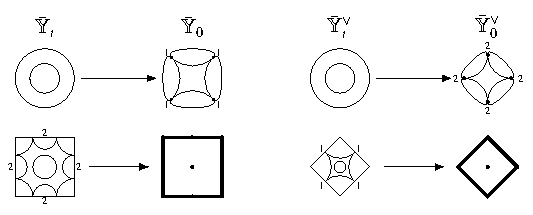
\includegraphics[width=0.96\textwidth]{figures/Fig_149_PDF257_Book245.pdf}
  \caption{例 8.29 中的对偶退化（原书 p.245）}
  \label{fig:elliptic-degeneration-polar-dual}
\end{figure}
\end{example}

这一思想在 Gross--Siebert 研究纲领中得到进一步发展与推广。其基本目标是通过一族簇研究镜像对称，这些簇退化为若干环簇之并，相邻的环簇沿轨道层相交。退化的交复形连同一些附加数据，可以通过离散 Legendre 变换重构镜像族。该方法使用代数几何、仿射结构、对数几何和热带几何中的许多技巧。关于这一纲领的更多内容，参见\bookcite{104,105,250}。

\section{练习}\label{sec:chapter-eight-exercises}

\begin{exercise}\label{exer:toric-line-bundle-cohomology}
设 $v_1,\ldots,v_4$ 是 $N=\mathbb Z^2$ 中的本原向量，它们把平面分为四个凸锥
\[
  \mathbb R_{\geq0}v_i+\mathbb R_{\geq0}v_{i+1}
\]
（下标按循环理解），并令 $\Delta$ 为对应的扇。对每个 $d\in\mathbb Z^4$，可在 $X_\Delta$ 上定义线丛 $\mathcal O(d)$。其 Čech 复形可按 $M=N^\vee$ 分次。请用几何方式，根据 $v_i,d_i$ 计算次数 $m\in M$ 部分的层上同调。
\end{exercise}

\begin{exercise}\label{exer:five-line-bundle-tilting}
设 $X$ 是由下图环簇图确定的完备环簇。
\begin{figure}[H]\centering
  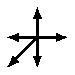
\includegraphics[width=0.17\textwidth]{figures/Fig_150_PDF258_Book246.pdf}
  \caption{练习 8.2 中的环簇图（原书 p.246）}
  \label{fig:exercise-eight-two-fan}
\end{figure}
说明为什么可以把 $X$ 看成在两个点处爆破的射影平面，或在一个点处爆破的 $\mathbb P^1\times\mathbb P^1$。找一个由五个形如 $\mathcal O(d)$ 的线丛直和组成的倾斜丛。
\end{exercise}

\begin{exercise}\label{exer:isolated-toric-singularity}
设 $v_1,\ldots,v_k\in\mathbb Z^2\times\{1\}$ 是位于高度 $1$ 的凸格点多边形 $\square$ 的顶点，令 $X^3_\square$ 是由锥
\[
  \sum_i\mathbb R_{\geq0}v_i
\]
对应的环簇。证明：$X^3_\square$ 有孤立奇点，当且仅当边上没有额外格点，且 $\square$ 不是基本三角形。
\end{exercise}

\begin{exercise}\label{exer:pick-theorem}
证明 Pick 定理：格点多边形的面积为
\[
  I+\frac{B}{2}-1,
\]
其中 $I$ 是内部格点数，$B$ 是边界格点数。
\end{exercise}

\begin{exercise}\label{exer:cyclic-quotient-toric-triangle}
固定 $(a,b)\in\mathbb Z^2$，令 $G=\langle g\mid g^n=1\rangle\cong\mathbb Z/n\mathbb Z$ 在 $\mathbb C^3$ 上的作用为
\[
  g(x,y,z)=\bigl(e^{2a\pi i/n}x,
  e^{2b\pi i/n}y,e^{-2(a+b)\pi i/n}z\bigr).
\]
证明该商可以描述为环簇 $X^3_\square$，其中 $\square$ 是面积为 $n/2$ 的三角形。
\end{exercise}

\begin{exercise}\label{exer:elliptic-tropicalization}
设椭圆曲线 $E$ 的方程为
\[
  Y^2=X^3+t^aX+t^b.
\]
描述其热带化如何随 $a,b\in\mathbb Z$ 变化。
\end{exercise}

\begin{exercise}\label{exer:one-polytope-three-dimensions}
第\ref{sec:one-two-three-mirror-symmetry}节为格点多边形在维数 $1,2,3$ 中构造了镜像。类似地，$n$ 维格点多面体也可在 $n-1,n,n+1$ 维中构造镜像。现在取 $n=1$。一维格点多面体就是长度为 $k$ 的线段 $L$，可将它放在 $\mathbb Z^2$ 中高度为 $1$ 的位置。
\begin{enumerate}[label=(\roman*)]
  \item 证明
  \[
    X^{n+1}_\square\cong V\bigl(\mathbb C[X,Y,Z]/(XY-Z^k)\bigr).
  \]
  描述消解 $X^{n+1}_{\boxtimes}\to X^{n+1}_\square$ 的例外纤维。
  \item $(n-1)$ 维镜像对应预言等价
  \[
    D^\pi\mathrm{MF}^{\pm}(X^{n+1}_{\boxtimes},\ell)
    \cong_\infty D^\pi_{\mathrm{wr}}\mathrm{Fuk}^{\pm}Y^{n-1}_\square.
  \]
  若把一点的 wrapped Fukaya 范畴解释为 $\mathrm{vect}^{\pm}_{\mathbb C}$，证明此对应成立。
  \item 对 $n$ 维版本，假设 $L$ 有一个内部格点。证明这会给出 $\mathbb P^1$ 的导出范畴与一个有向 Fukaya 范畴之间的镜像对应，并给出证明策略。
  \item 对 $(n+1)$ 维版本，描述支撑在 $\mathbb P^1$ 上的 $X^{n+1}_{\boxtimes}$ 上的层导出范畴。证明它与代数
  \[
    \mathbb C[[X,Y]]\star\mathbb Z_2
  \]
  的有限维模导出范畴等价，其中 $\mathbb Z_2$ 对 $X,Y$ 都按符号作用。
\end{enumerate}
\end{exercise}

\begin{exercise}\label{exer:genus-g-toric-triangle}
调整亏格为 $g$ 的曲线的镜像构造，使它适用于任意一个内部有 $g$ 个格点、边界上没有格点的格点三角形。
\begin{enumerate}[label=(\roman*)]
  \item 证明：当 $g=2$ 时，这种构造总是给出 Seidel 的同一构造。
  \item 证明：当 $g=3$ 时，存在不止一种可能（即在格的自同构意义下有不同的三角形）。哪一种对应 Efimov 的构造？
  \item 详细研究一个 $g=3$、但不对应 Efimov 构造的三角形。描述群作用，并确定商奇点的不同可能消解。
\end{enumerate}
\end{exercise}

\begin{exercise}\label{exer:batyrev-elliptic-curve-p1-p1}
用齐次坐标 $((X:Y),(U:V))$ 描述空间 $\mathbb P^1\times\mathbb P^1$。证明：对通有的 $q$，方程
\[
  XYUV+q(X^2+Y^2)(U^2+V^2)=0
\]
的零点集是一条椭圆曲线。用 Batyrev 对偶的观点解释这一构造。
\end{exercise}

\begin{exercise}\label{exer:lg-lg-an-singularity}
为简单奇点 Landau--Ginzburg 模型
\[
  X=(\mathbb A^n,X_1^2+\cdots+X_n^2)
\]
构造 Landau--Ginzburg 镜像 $Y$，并双向证明镜像对称：$X$ 的 $A$ 模型等价于 $Y$ 的 $B$ 模型，反过来也成立。
\end{exercise}

\chapterreview{%
\textbf{全章地位。}前七章分别造出 $A$ 侧与 $B$ 侧的范畴，本章第一次把它们真正对上。作者没有直接处理紧致 Calabi--Yau 流形，而是从 $(\mathbb C^*)^n$ 与 $T^*(S^1)^n$ 这对最简单的镜像出发，逐步加入环簇与热带几何，最后把一、二、三维的构造统一成“Newton 多边形 $+$ 三角剖分”这组组合数据。后半转向 SYZ 猜想与 Gross--Siebert 纲领。

\textbf{知识脉络。}线索是“一个例子、两种几何、三个维数、一个猜想”。§8.1 用复环面把 wrapped、正合、$\mathbb Z_2$ 分次三种 Fukaya 范畴分别对应凝聚层、挠层与矩阵分解；§8.2 引入环簇，把“锥 $-$ 轨道 $-$ 除子”的字典翻译成“势函数单项式”；§8.3 用热带几何把 $t\to\infty$ 的阿米巴极限化为 Newton 多边形的对偶三角剖分；§8.4 陈述一、二、三维的镜像等价；§8.5 讨论离开大体积极限后如何紧化、加除子并加入极端单项式；§8.6 用 SYZ 纤维化解释镜像对的整体几何。

\textbf{核心结论。}（1）$D^\infty\mathrm{wrFuk}^{\bullet}(T^*(S^1)^n)\cong D\mathrm{Coh}^{\bullet}(\mathbb C^*)^n$，正合版本对应挠层，$\mathbb Z_2$ 分次版本对应 $\mathrm{MF}^{\pm}(\mathbb C^{n+2},(X_0\cdots X_n-1)Z)$；镜像上的点对应底环面 $(S^1)^n$ 上的一维局部系统，故镜像是作为对偶群出现的 $T^\vee=\operatorname{Grp}(N,\mathbb C^*)$。（2）环簇中锥与轨道一一对应，$\dim\sigma=n-\dim O_\sigma$；一维锥给出射线向量 $v_\sigma$ 与环簇除子 $D_\sigma$，$A$ 侧加入 $D_\sigma$ 恰使 $B$ 侧势函数多出单项式 $y^{v_\sigma}$，即 $W_\hbar=\sum\hbar\,y^{v_\sigma}$。（3）热带极限把几何变成组合：$W_t^{-1}(0)$ 的亏格等于 Newton 多边形的内部格点数，穿孔数等于边界格点数，三角剖分与热带曲线对偶。（4）三维对应有三条：$D^\pi\mathrm{MF}^{\pm}X^1_{\boxtimes}\simeq D^\pi\mathrm{wrFuk}^{\pm}Y^1_\square$；$D\mathrm{Coh}^{\bullet}X^2_v\hookrightarrow D^\pi\mathrm{drFuk}^{\bullet}Y^2_\square$；$D\mathrm{Coh}^{\bullet}_{X^2_v}(X^3_{\boxtimes})\hookrightarrow D^\pi\mathrm{exFuk}^{\bullet}Y^3_\square$，其中第二条在内部格点唯一（$X^2_v=\ell^{-1}(0)$）时升级为等价。

\textbf{辨析与提醒。}其一，“环簇”不是“环面”：环簇是含稠密复环面开轨道、由扇组合定义的正规簇，复环面只是它的一个开子集；“环簇除子”专指余维 $1$ 轨道闭包。其二，几种 Fukaya 范畴不要混：wrapped 用于非紧余切丛，正合用于紧正合拉格朗日，有向用于 LG 模型的盘，相对版本 $\mathrm{cuFuk}$ 用于带除子的流形，partially wrapped 则带 stop。其三，$t\to\infty$ 的热带极限与 $\hbar\to0$ 是同一退化的两种说法，阿米巴“收敛到”热带曲线是 Hausdorff 意义下的收敛，不能当作相等。其四，大体积极限丢掉紧致性与 Kähler 模：恢复紧致须紧化并加除子，所得范畴定义在 $\mathbb C[[q_1,\ldots,q_r]]$ 上，两侧参数只由形式幂级数环的自同构联系，不要指望逐一对应。

\textbf{评注。}作者的策略是用环簇与热带几何绕开一般 Calabi--Yau 流形上难以构造的特殊拉格朗日纤维化，把镜像对称化归为多边形与三角剖分的组合游戏。代价是结论基本停留在大体积极限与非紧流形，真正紧的情形只剩 SYZ 猜想与 Gross--Siebert 纲领的入口。三维部分的拆法值得注意：$B$ 侧分成 $X^1_{\boxtimes}$、$X^2_v$、$X^3_{\boxtimes}$ 三层，分别对应矩阵分解、凝聚层与支撑层，看似重复，实则正是 Abouzaid 等人“先找分裂生成元、再比自同态代数”的证明路线；三行对应当读成一个构造的三层，而非三个独立定理。椭圆曲线与极对偶两小节把 Batyrev 对偶放进同调框架，是连接经典镜像对称与范畴版本的桥梁，也是本章最值得细读之处。}


\part{曲面上的思考}
\chapter{粘合}\label{ch:gluing}
本章将引入一种 $A_\infty$ 范畴，作为曲面上 partially wrapped Fukaya 范畴的一个模型。这种拓扑 Fukaya 范畴的优点在于，它可以由曲面剖分成多边形后组合地构造出来，而不必处理真正 Fukaya 范畴定义中诸多棘手的技术问题。

具体来说，这个范畴被定义为某个 $A_\infty$ 代数的导出范畴；该代数由曲面的多边形剖分得到。它与表示论中研究甚广的两类特殊代数密切相关：双列代数\bookcite{88,234}和 gentle 代数\bookcite{14,208}。对这一范畴作 Fukaya 范畴解释，可以从曲面上的曲线角度，为这些代数的表示论带来新的理解\bookcite{166}。

还可以通过不同方式把较小的范畴粘合起来，构造这些范畴\bookcite{115,65,204,189,232}。本章将讨论这种现象并给出若干例子。这些粘合方法也能用来构造此类范畴的 $B$ 侧镜像，即 Landau--Ginzburg 模型\bookcite{204,155}。这属于 Kontsevich\bookcite{144} 发起的一项更广泛研究计划：把 wrapped Fukaya 范畴视为定义在拉格朗日骨架上的范畴层。

文献中出现过这些范畴的多个版本\bookcite{3,156,115,65,204,36,166,155}；它们在允许的曲面类型、采用 $\mathbb Z_2$ 分次还是 $\mathbb Z$ 分次上，有不同约定与限制。本章聚焦于 $\mathbb Z_2$ 分次版本，下一章再转向 $\mathbb Z$ 分次情形。

\section{带标记曲面}\label{sec:marked-surfaces}
\takeaway{带标记曲面连同生成弧系给出 gentle $A_\infty$ 代数 $\mathrm{Gtl}^{\pm}A$ 与箭图 $Q_A$；高阶乘积由边界为弧的浸入多边形计数，拓扑 Fukaya 范畴 $\mathrm{topFuk}^{\pm}$ 定义为其导出范畴，且与弧系的选取无关。}
\begin{definition}{带标记曲面}{marked-surface}
带标记曲面\index{daibiaojiqumian@带标记曲面|hyperpage} $(S,M)$ 由紧致定向曲面 $S$ 和有限点集 $M\subset S$ 构成。曲面可以有边界分支 $B_1,\ldots,B_k$，并要求每个连通分支和每个边界分支上都至少有一个 $M$ 中的点。位于边界上的点称为边界标记点，位于曲面内部的点称为内部标记点。
\end{definition}

\begin{definition}{弧、同位变形与不相交性}{arc}
弧\index{hu@弧|hyperpage}是连接标记点的嵌入曲线 $a\colon[0,1]\to S$，并且中间不经过任何标记点，即 $a^{-1}(M)=\{0,1\}$，也不围成一个没有内部标记点的圆盘。\footnote{换言之，我们不考虑可缩弧。}若两个弧可以通过一参数弧族彼此变形，则称它们同位变形。若两条弧除端点外不相交，则称它们不相交。
\end{definition}

\begin{definition}{生成弧系}{generating-arc-collection}
一组两两不相交、且任意两条都不能通过同位变形互相变换的弧，称为生成弧系\index{shengchenghuxi@生成弧系|hyperpage}，若任意其他弧都可以通过同位变形变为该弧系中若干条首尾相接的弧（忽略方向）组成的序列。也说这组弧剖分了曲面。
\end{definition}

\begin{note}\label{note:open-closed-polygons}
沿生成弧系切开曲面后，曲面会分解为若干多边形，其顶点是标记点，边要么是弧，要么是边界的一段。对每个多边形而言，边要么全是弧，要么除一条外全是弧；否则，连接两条非弧边的对角线无法同位变形为弧的序列。若多边形的每条边都是弧，就称其为闭多边形\index{biduobianxing@闭多边形|hyperpage}；若恰有一条边不是弧，则称其为开多边形\index{kaiduobianxing@开多边形|hyperpage}。
\end{note}

给定生成弧系 $A$，可以构造箭图 $Q_A$。它的顶点是弧，即 $(Q_A)_0=A$；箭是多边形中这些弧之间的角。具体地，在标记点周围画一个小圆（若标记点在边界上，则画半圆）。弧把圆周切成若干小段，将这些小段按逆时针方向定向；每一段若连接两条弧，就在 $Q_A$ 中画一条箭 $\alpha$。

\begin{example}[生成弧系与相应箭图]
下图给出六标记圆盘的三种生成弧系与三标记环带的两种生成弧系，并画出相应的箭图。
\begin{figure}[H]\centering
  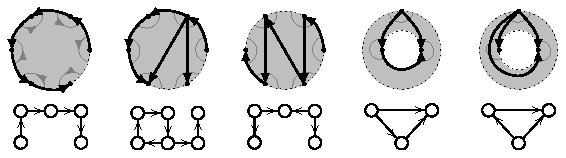
\includegraphics[width=0.89\textwidth]{figures/Fig_151_PDF265_Book253.pdf}
  \caption{生成弧系及其箭图（原书 p.253）}\label{fig:arc-collections-quivers}
\end{figure}
\end{example}

对每个弧系，其箭图都有一个特殊性质：每个顶点至多有两条入箭和两条出箭。因此，对每条箭 $\beta$，以 $\beta$ 开始的长度为 $2$ 的路径至多有两条。若路径 $\alpha\beta$ 中的两角在标记点周围的圆上相邻，就称它为角状路径\index{jiaozhuanglujing@角状路径|hyperpage}；若两角在多边形内相邻，则称它为面状路径\index{mianzhuanglujing@面状路径|hyperpage}。分别记角状路径集为 $P^+$（它们绕标记点逆时针转向）和面状路径集为 $P^-$（它们绕多边形顺时针转向）。

\begin{figure}[H]\centering
  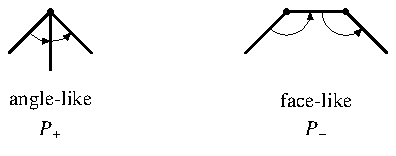
\includegraphics[width=0.48\textwidth]{figures/Fig_152_PDF265_Book253.pdf}
  \caption{角状路径与面状路径（原书 p.253）}\label{fig:angle-like-face-like}
\end{figure}

\begin{definition}{弧系的 gentle $A_\infty$ 代数}{gentle-a-infinity-algebra}\index{gentleadaishu@gentle $A_\infty$ 代数|hyperpage}
弧系的 gentle $A_\infty$ 代数是箭图 $Q_A$ 的路径代数除以面状路径所生成的理想：
\[
  \mathrm{Gtl}^{\pm}A:=\frac{\mathbb C Q_A}{\langle\alpha\beta\mid\alpha\beta\in P^-\rangle}.
\]
它的 $\mathbb Z_2$ 分次按下图规则赋予：
\begin{figure}[H]\centering
  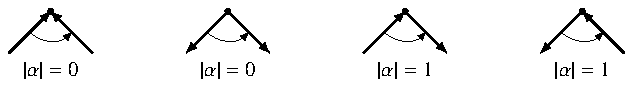
\includegraphics[width=0.65\textwidth]{figures/Fig_153_PDF265_Book253.pdf}
  \caption{弧系箭的 $\mathbb Z_2$ 次数（原书 p.253）}\label{fig:arc-degree-rule}
\end{figure}
在 $\mathrm{Gtl}^{\pm}A$ 上定义如下 $A_\infty$ 结构：若 $\beta_1,\ldots,\beta_l$ 是一个无内部标记点、边界由弧组成的浸入多边形上的连续各角，则
\[
  \mu(\alpha\beta_1,\beta_2,\ldots,\beta_k)=\alpha,
  \qquad
  \mu(\beta_1,\ldots,\beta_k\gamma)=(-1)^{|\gamma|}\gamma.
\]
% [Tutor Note: 定义正文说 $\beta_1,\ldots,\beta_l$ 是一个多边形的连续各角，两条乘积公式却写成 $\beta_k$；原书 p.253 此处指标不一致，按上下文两处应指同一组角，代入时以正文的 $\beta_l$ 为准。]
\end{definition}

\begin{figure}[H]\centering
  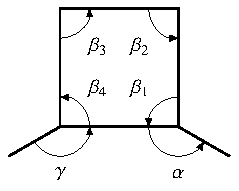
\includegraphics[width=0.44\textwidth]{figures/Fig_154_PDF266_Book254.pdf}
  \caption{高阶乘积的边界角（原书 p.254）}\label{fig:gentle-product-four-gon}
\end{figure}

\begin{lemma}{gentle 代数上的高阶乘积定义了 $A_\infty$ 结构}{gentle-algebra-ainfty-structure}
上述规则定义了一个 $A_\infty$ 结构\bookcite{115,36}。
\end{lemma}
\begin{proof}[证明思路]
首先，乘积的 $\mathbb Z_2$ 次数正确。若 $\alpha_1,\ldots,\alpha_k$ 位于某个多边形上，且所有弧沿多边形的方向一致，则所有 $\alpha_i$ 的次数都是 $1$。删去这些弧时，次数变化为 $k$；在 $\mathbb Z_2$ 中这与 $2-k$ 相同。若改变一条弧的方向，则有两个 $\alpha_i$ 的次数改变 $1$，总次数模 $2$ 不变。

下面验证 $A_\infty$ 关系。若
\[
\mu\bigl(\alpha_1,\ldots,\alpha_k,\mu(\alpha_{k+1},\ldots,\alpha_l),\ldots,\alpha_n\bigr)\ne0,
\]
根据内外两层乘积是否为二元乘积，可分为四种情形。
\begin{itemize}
  \item 若两者都是二元乘积，这就是普通乘积的结合律。
  \item 若外层乘积是二元乘积，则有
  \[
    \mu\bigl(\alpha_1,\mu(\alpha_2\beta_1,\ldots,\beta_k)\bigr)
    -\mu\bigl(\mu(\alpha_1,\alpha_2\beta_1),\ldots,\beta_k\bigr)=0.
  \]
  相应的两项来自同一多边形的两种分解：
  \begin{figure}[H]\centering
    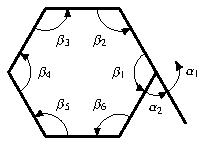
\includegraphics[width=0.42\textwidth]{figures/Fig_155_PDF266_Book254.pdf}
    \caption{外层乘积为二元乘积时的抵消（原书 p.254）}\label{fig:ainfty-cancellation-outer}
  \end{figure}
  \item 若内层乘积是二元乘积，则位于内层中间的弧把浸入多边形分成两个多边形，从而得到两个非零高阶乘积项，二者相消。
  \item 若内外两层都是高阶乘积，这两个多边形粘合成一个较大的浸入圆盘；相应地会出现一个内层为二元乘积的非零项，与原项相消：
  \begin{figure}[H]\centering
    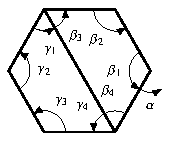
\includegraphics[width=0.48\textwidth]{figures/Fig_156_PDF266_Book254.pdf}
    \caption{两个高阶乘积对应的抵消项（原书 p.254）}\label{fig:ainfty-cancellation-higher}
  \end{figure}
  \[
    \mu(\alpha\beta_1,\beta_2,\mu(\beta_3\gamma_1,\gamma_2,\gamma_3,\gamma_4),\beta_4)
    -\mu(\alpha\beta_1,\beta_2,\beta_3\gamma_1,\gamma_2,\gamma_3,\mu(\gamma_4,\beta_4))=0.
  \]
\end{itemize}
每种情形中恰有两个非零项，并且它们互相抵消。\hfill$\square$
\end{proof}

\begin{lemma}{高阶乘积与有限维性}{gentle-algebra-finiteness}
设 $A$ 是剖分曲面的弧\index{poufenqumiandehu@剖分曲面的弧|hyperpage}系，$(\mathrm{Gtl}^{\pm}A,\mu)$ 是相应的 gentle $A_\infty$ 代数。
\begin{enumerate}[label=(\roman*)]
  \item 高阶乘积全为零，当且仅当不存在闭多边形。
  \item gentle 代数有限维，当且仅当不存在内部标记点。
\end{enumerate}
\end{lemma}
\begin{proof}[证明思路]
每个非零高阶乘积都来自一个边界由弧组成的浸入多边形。这样的多边形必由若干闭多边形粘合而成。gentle 代数中的非零路径对应标记点周围的角；若标记点在内部，这些角可以无限次地连续转绕。\hfill$\square$
\end{proof}
% [Tutor Note: 第一条的“当且仅当”要两边验证：若存在闭多边形，其各角按规则相乘得到 $\lambda\,1_a$（$\lambda\ne0$），故有非零高阶乘积；反之任何非零高阶乘积所在浸入多边形的边界都由闭多边形拼成。]

\begin{example}[含内部标记点的圆盘]
取一个圆盘，内部有 $k$ 个标记点，边界上有 $l$ 个标记点。把一个内部标记点连接到所有其他标记点。所得箭图是一个循环箭图；连接两个内部点的弧所对应的顶点上带有环。所有箭的次数均为 $0$，环与其他箭的乘积为零。该 gentle 代数是无限维的，但没有高阶乘积。
\begin{figure}[H]\centering
  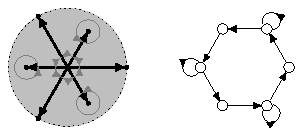
\includegraphics[width=0.43\textwidth]{figures/Fig_157_PDF267_Book255.pdf}
  % [Fig] 原书 p.255
\end{figure}
\end{example}

若考虑内圈和外圈各有 $k$ 个标记点的环带，可以用之字形弧将内外标记点相连。由此得到的循环箭图中箭的方向交替变化。此时没有关系，也没有高阶乘积，因此 gentle 代数就是路径代数。
\begin{figure}[H]\centering
  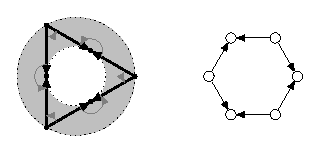
\includegraphics[width=0.43\textwidth]{figures/Fig_158_PDF267_Book255.pdf}
  % [Fig] 原书 p.255
\end{figure}

\begin{note}\label{note:gentle-algebra-classical}
gentle 代数最初由 Assem 和 Skowroński 在文献\bookcite{14}中引入，指满足下列条件的一类无分次路径代数 $\mathbb C Q/I$：
\begin{enumerate}[label=(G\arabic*)]
  \item $Q$ 没有有向环，且每个顶点至多有两条入箭和两条出箭；
  \item $I$ 由长度为 $2$ 的路径生成；
  \item 对每条箭 $\alpha\in Q_1$，至多有一条路径 $\alpha\beta$ 属于 $I$，也至多有一条路径 $\gamma\alpha$ 属于 $I$；
  \item 对每条箭 $\alpha$，至多有一条路径 $\alpha\beta$ 不属于 $I$，也至多有一条路径 $\gamma\alpha$ 不属于 $I$。
\end{enumerate}
引入这类代数，是因为它们具有良好的表示论性质，因而可以分类其不可分解表示。它们与镜像对称的联系则是后来才发现的\bookcite{3,36,115,166}。
\end{note}

\begin{theorem}{Lekili--Polishchuk 定理}{gentle-algebras-from-surfaces}
每个上述意义下的 gentle 代数都来自某个曲面。\bookcite{166}\footnote{这是 Lekili 与 Polishchuk 定理的一个特例；他们的结果处理的是 $\mathbb Z$ 分次版本。}
\end{theorem}
\begin{proof}[证明思路]
我们分步构造曲面。
\begin{enumerate}[label=(\roman*)]
  \item 考虑所有满足 $\alpha_i\alpha_{i+1}\in I$ 的最长序列 $\alpha_1\cdots\alpha_k$。对每个这样的序列取一个 $(k+2)$ 边形，并按 $h(\alpha_1),h(\alpha_2),\ldots,h(\alpha_k),t(\alpha_k)$ 给除最后一条边以外的边标记。将箭画成沿多边形角落排列的小角。由 (G3)，每条箭恰好属于一个多边形。
  \item 考虑所有满足 $\beta_i\beta_{i+1}\notin I$ 的最长序列 $\beta_1\cdots\beta_k$。对每个这样的序列取一个标记点 $m_i$，并把每个多边形的角标为包含该角的序列所对应的标记点。
  \item 沿着具有相同标记的边与角粘合多边形。所得曲面可定向，因为各多边形上的角均顺时针排列，而标记点周围的角均逆时针排列。
  \item 定向各条边，使每个标记点处的边要么全部指向该点，要么全部从该点指出。
\end{enumerate}
这样得到一个弧系，它把曲面剖分为开多边形。相应的 gentle $A_\infty$ 代数集中在次数 $0$，没有高阶乘积，并且同构于 $\mathbb C Q/I$。\hfill$\square$
\end{proof}

\begin{theorem}{生成弧系改变时的拟等价}{gentle-derived-invariance}
同一带标记曲面的两个生成弧系所对应的 gentle $A_\infty$ 代数，其扭曲完备化彼此 $A_\infty$ 拟等价\bookcite{115,36}。
\end{theorem}
\begin{proof}[证明思路]
若 $A'$ 是把弧 $a$ 的方向反转后由 $A$ 得到的，则可以把 $\mathrm{Gtl}^{\pm}A'$ 嵌入 $\mathrm{TwGtl}^{\pm}A$，方法是把反向弧识别为对象 $a[1]$（注意，$a$ 是 $Q_A$ 的顶点，因而也是范畴 $\mathrm{Gtl}^{\pm}A$ 的对象）。

若 $A$ 与 $A'=A\cup\{a\}$ 都是剖分曲面的弧系，则 $a$ 位于 $A$ 的某个多边形内，并可找到一列弧 $a_1,\ldots,a_k$，其首尾相接后可同位变形为 $a$：
\begin{figure}[H]\centering
  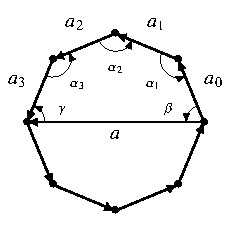
\includegraphics[width=0.62\textwidth]{figures/Fig_159_PDF269_Book257.pdf}
  \caption{把新增弧表示为扭曲复形（原书 p.257）}\label{fig:added-arc-twisted-complex}
\end{figure}
在范畴 $\mathrm{TwGtl}^{\pm}A'$ 中，对象 $a$ 与下列对象拟同构：
\[
  M=(a_0\oplus\cdots\oplus a_k,\alpha_1+\cdots+\alpha_k).
\]
事实上，设 $\beta$ 是 $a_0$ 与 $a$ 之间的角，$\gamma$ 是 $a$ 与 $a_k$ 之间的角，则 $\beta\in\mathrm{TwGtl}^{\pm}A'(M,a)$、$\gamma\in\mathrm{TwGtl}^{\pm}A'(a,M)$ 互为逆元，因为
\[
  \widehat\mu_2(\beta,\gamma)=\mu(\beta,\alpha_0,\ldots,\alpha_k,\gamma)=1_a,
\]
\[
  \widehat\mu_2(\gamma,\beta)=\sum_i\mu(\alpha_i,\ldots,\alpha_k,\gamma,\beta,\alpha_0,\ldots,\alpha_{i-1})
  =1_{a_1}+\cdots+1_{a_k}=1_M.
\]
因此，$\mathrm{Gtl}^{\pm}A$ 生成 $\mathrm{TwGtl}^{\pm}A'$。

只要两组弧都剖分曲面，添加或删除一条弧就不会改变扭曲完备化。不断添加弧，可将任一弧系扩充为曲面的三角剖分。Hatcher 定理\bookcite{110}说明，任意两个三角剖分都可以通过四边形中翻转对角线的操作互相转化（即删去一条对角线并以另一条替代）。
\begin{figure}[H]\centering
  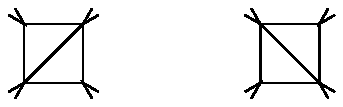
\includegraphics[width=0.36\textwidth]{figures/Fig_160_PDF269_Book257.pdf}
  \caption{翻转四边形的对角线（原书 p.257）}\label{fig:flip-diagonal}
\end{figure}
由此即可得到结论。\hfill$\square$
\end{proof}

\begin{definition}{带标记曲面的拓扑 Fukaya 范畴}{topological-fukaya-marked-surface}
带标记曲面 $(S,M)$ 的 $\mathbb Z_2$ 分次拓扑 Fukaya 范畴\index{tuopufukayafanchou@拓扑 Fukaya 范畴|hyperpage}，定义为任一剖分弧系 $A$ 所对应的 gentle $A_\infty$ 范畴的导出范畴：
\[
  \mathrm{topFuk}^{\pm}(S,M):=D\mathrm{Gtl}^{\pm}A.
\]
\end{definition}

\begin{example}[三类经典箭图]
第四章研究过的线性箭图、Kronecker 箭图和循环箭图，都属于这一框架。它们的导出范畴分别等价于下列带标记曲面的拓扑 Fukaya 范畴：边界上有 $n$ 个标记点的圆盘；两个边界分支上各有一个标记点的圆柱；内部有一个标记点、边界上有 $n$ 个标记点的圆盘。
\end{example}

\begin{note}\label{note:marked-surface-conventions}
文献中对带标记曲面有不同约定，差异在于如何处理标记点和边界分支：
\begin{enumerate}[label=(\roman*)]
  \item 文献\bookcite{3,156,36}采用与本书相同的约定。
  \item 在文献\bookcite{115}中，标记点被切除。内部标记点变成一个小的标记边界圆；带有 $n$ 个标记点的边界分支变成由 $2n$ 段组成的边界，标记段和非标记段交替排列。弧的端点落在标记边界段上；不同弧的端点彼此不同（但可以落在同一标记段上），角则是这些标记边界段的子段。角也称为 Reeb 弦。
  \item 在文献\bookcite{166}中，边界的非标记段被压缩成点，并称作 stop（文献中有时也管它叫标记点，容易混淆），因为它们会阻碍 Reeb 弦的流动。
  \item 在文献\bookcite{204}中，采用带状图的对偶形式（见定义\ref{def:ribbon-graph}）。每个多边形的中心成为带状图的一个节点，并与多边形的各边相连，构成带状图的半边。
\end{enumerate}
\begin{figure}[H]\centering
  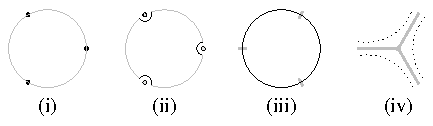
\includegraphics[width=0.9\textwidth]{figures/Fig_161_PDF270_Book258.pdf}
  \caption{四种带标记曲面的约定（原书 p.258）}\label{fig:marked-surface-conventions}
\end{figure}
\end{note}

\begin{note}\label{note:marked-surface-generalizations}
带标记曲面的概念还有一些有时很有用的推广。
\begin{itemize}
  \item \textbf{同位变形的弧。}若弧 $a,b$ 可以通过同位变形互相变换，则它们围成一个二边形。若把高阶乘积规则扩展到二边形，就会得到 $\mu_2(\alpha,\beta)=\pm1_a$ 和 $\mu_2(\beta,\alpha)=\pm1_b$，因此 $a,b$ 是同构对象。含有 $a,b$ 两条弧的集合严格说来不再给出 gentle 代数，但所得代数与只含 $a$ 的 gentle 代数 Morita 等价。二边形见图\ref{fig:isotopic-arcs-digon}。
  \begin{figure}[H]\centering
    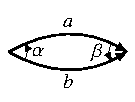
\includegraphics[width=0.18\textwidth]{figures/Fig_162_PDF271_Book259.pdf}
    \caption{同位变形的弧围成二边形（原书 p.259）}\label{fig:isotopic-arcs-digon}
  \end{figure}
  \item \textbf{曲面中的穿孔。}可以把穿孔建模为 $S\setminus M$ 内部的另一组点 $P$。弧不得经过这些点，也不得以它们为端点；生成弧系的每个多边形至多包含一个穿孔。定义高阶乘积时，只考虑不覆盖穿孔的浸入多边形。
  \item \textbf{轨形点。}可以把轨形点建模为 $S\setminus M$ 内部的点 $o_i$，并给每个点赋予次数 $d_i\ge2$。弧不得经过这些点，也不得以它们为端点；生成弧系的每个多边形至多包含一个轨形点。若多边形含有次数为 $d_i$ 的轨形点，则要求
  \[
    \mu(\underbrace{\beta_1,\ldots,\beta_k,\ldots,\beta_1,\ldots,\beta_k}_{d_i\text{ 次}})=h(\beta_1),
  \]
  其中 $\beta_1,\ldots,\beta_k$ 是该多边形的各角。其他乘积可以通过提升到轨形万有覆盖来计算。
  \item \textbf{面积。}若给每个多边形赋予面积，则可以用因子 $e^{-A}$ 对高阶乘积 $\mu$ 加权，其中 $A$ 是浸入多边形的总面积。通常可通过 gentle 代数的自同构消去这些面积参数。
\end{itemize}
\end{note}

\section{从弧到弦与带}\label{sec:arcs-strings-bands}
\takeaway{把首尾相接的弧用角缝合，开曲线实现为扭曲复形上的弦对象，闭曲线实现为带局部系统的带对象；交点是态射，曲线围成的多边形计数高阶乘积，故 $\mathrm{topFuk}^{\pm}$ 可看作 Fukaya 范畴的组合模型。}
称 $\mathrm{topFuk}^{\pm}(S,M)$ 为拓扑 Fukaya 范畴，是因为其中的对象可以与曲面上开曲线和闭曲线的同伦类对应。本节将说明如何把这类对象构造为 gentle $A_\infty$ 代数上的扭曲复形。更多细节见\bookcite{115,36,37}。

考虑一列弧 $a_1[i_1],\ldots,a_k[i_k]$，其中各弧经过平移后首尾相接。对每对相邻弧 $a_u[i_u]$ 与 $a_{u+1}[i_{u+1}]$，选取一个绕公共标记点的角 $\alpha_u$；它可以从 $a_u$ 指向 $a_{u+1}$，也可以反向。注意，$\alpha_u$ 可视为 $a_u[i_u]$ 到 $a_{u+1}[i_{u+1}]$ 或反向的次数为 $1$ 的态射。由此可定义两个对象：
\begin{itemize}
  \item 在曲面 $S$ 上，用沿角 $\alpha_u$ 的小弦把各弧缝合，得到浸入曲线 $L$；
  \item 在 $\mathrm{TwGtl}^{\pm}A$ 中定义复形
  \[
    (L,\delta):=\left(\bigoplus_{j=1}^k a_j[i_j],\ \sum_{u=1}^{k-1}\alpha_u\right).
  \]
\end{itemize}
曲线 $L$ 的几何性质与相应扭曲复形的代数性质紧密相关。
\begin{figure}[H]\centering
  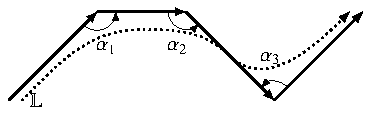
\includegraphics[width=0.52\textwidth]{figures/Fig_163_PDF272_Book260.pdf}
  \caption{用弧与角拼接出曲线及其扭曲复形（原书 p.260）}\label{fig:string-from-arcs}
\end{figure}

\begin{lemma}{开弦对象的基本性质}{string-object-properties}
设 $L$ 是一条曲线，$(L,\delta)$ 是与之对应的扭曲复形。
\begin{enumerate}[label=(\roman*)]
  \item $(L,\delta)$ 满足 Maurer--Cartan 方程，当且仅当 $L$ 不含在 $S\setminus M$ 中可缩的环；
  \item 与彼此同位变形的曲线对应的扭曲复形在 $\mathrm{topFuk}^{\pm}(S,M)$ 中同构；
  \item 对每个同伦类，都存在一列弧，使其缝合得到属于该同伦类的曲线 $L$。
\end{enumerate}
\end{lemma}
\begin{proof}[证明思路]
若存在可缩环，则环内各角 $\alpha_u$ 会给出非零乘积 $\mu(\alpha_u,\ldots,\alpha_v)$。若不存在可缩环，则 Maurer--Cartan 方程中的所有高阶乘积均为零。普通乘积也全为零：扭曲微分 $\delta$ 中相邻的两个角要么不可复合，要么其乘积由 gentle 代数中的关系置零。
相邻角的两种情形如下：
\begin{figure}[H]\centering
  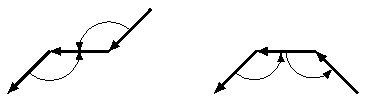
\includegraphics[width=0.5\textwidth]{figures/Fig_164_PDF272_Book260.pdf}
  \caption{相邻角的乘积为零的两种情形（原书 p.260）}\label{fig:consecutive-string-angles}
\end{figure}

为证第二条，考虑两列只在某一个多边形处不同的弧序列：一列沿多边形顺时针绕行，另一列沿逆时针绕行。由此得到扭曲对象 $(L_1,\delta_1)$ 与 $(L_2,\delta_2)$。令 $u=\sum 1_a+\beta_1\in\mathrm{Hom}^{\bullet}(L_1,L_2)$、$v=\sum 1_a+\beta_2\in\mathrm{Hom}^{\bullet}(L_2,L_1)$，其中求和遍历 $L_1,L_2$ 的公共箭。计算扭曲乘积时，插入多边形各角会产生额外的高阶乘积项；结果为
\[
\begin{aligned}
\widehat\mu(u,v)
&=\sum_{a\in L_1\cap L_2}1_a+
\sum\mu\bigl(\cdots\alpha_i^{L_2}\cdots,\beta_1,
\cdots\alpha_i^{L_1}\cdots,\beta_2,\cdots\alpha_i^{L_2}\cdots\bigr)\\
&=\sum_{a\in L_1\cap L_2}1_a+
\sum_{a\in L_2\setminus L_1}1_a=1_{L_2}.
\end{aligned}
\]
反向乘积同理，因此 $u,v$ 互为逆元。两条彼此同位变形的曲线之间的局部变换如下：
\begin{figure}[H]\centering
  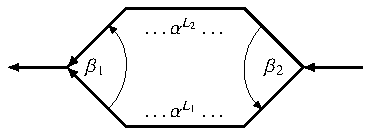
\includegraphics[width=0.52\textwidth]{figures/Fig_165_PDF273_Book261.pdf}
  \caption{在多边形内改变弧的绕行方向（原书 p.261）}\label{fig:isotopy-string-curves}
\end{figure}
任意两条彼此同位变形的曲线都可以通过一系列这类局部变换互相得到。

为证第三条，先对曲线作同位变形，使其不含可缩环；再把曲线每次穿过多边形的线段替换为沿多边形顺时针或逆时针绕行的弧序列，并用多边形内的角把各箭缝合起来。\hfill$\square$
\end{proof}

\begin{definition}{弦对象}{string-object}
连接两个标记点的曲线 $L$ 所对应的弦对象\index{xianduixiang@弦对象|hyperpage} $S(L)$，是由一列近似该曲线的弧所得到的扭曲对象 $(L,\delta)$。
\end{definition}

\begin{lemma}{弦对象的自同态空间}{string-object-endomorphisms}
设 $a$ 是连接两个不同标记点 $p_1,p_2$ 的弧。
\begin{enumerate}[label=(\roman*)]
  \item 若 $p_1,p_2$ 都是内部点，则
  \[
    \mathrm{topFuk}^{\pm}(S(a),S(a))\cong k[\ell_1,\ell_2]/(\ell_1\ell_2).
  \]
  \item 若只有 $p_1$ 是内部点，则 $\mathrm{topFuk}^{\pm}(S(a),S(a))\cong k[\ell_1]$。
  \item 若 $p_1,p_2$ 都在边界上，则 $\mathrm{topFuk}^{\pm}(S(a),S(a))\cong k$。
\end{enumerate}
\end{lemma}
\begin{proof}[证明思路]
取一个包含 $a$ 的弧系，并构造 gentle 代数 $\mathrm{Gtl}^{\pm}A$。第一种情形下，
\[
  \mathrm{topFuk}^{\pm}(S(a),S(a))=1_a\cdot\mathrm{Gtl}^{\pm}A\cdot1_a.
\]
这个空间由所有从 $e_a$ 出发的非零环路张成。基本环路有两个：$\ell_1$ 绕过 $a$ 的头端，$\ell_2$ 绕过尾端；它们的乘积由 gentle 代数中的关系置零。其余情形类似。
\begin{figure}[H]\centering
  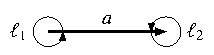
\includegraphics[width=0.42\textwidth]{figures/Fig_166_PDF273_Book261.pdf}
  \caption{弧两端的基本环路（原书 p.261）}\label{fig:string-end-loops}
\end{figure}
\hfill$\square$
\end{proof}

闭曲线也能构造出对象。先取一列首尾相接成环的弧 $a_1[i_1],\ldots,a_k[i_k]$，再用角 $\alpha_u$ 缝合它们，得到闭曲线 $L$。此时还需一个角 $\alpha_k$ 连接 $a_k$ 与 $a_1$。图中画出由此得到的曲线：
\begin{figure}[H]\centering
  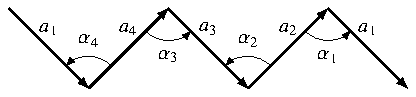
\includegraphics[width=0.52\textwidth]{figures/Fig_167_PDF275_Book263.pdf}
  \caption{用弧与角拼接闭曲线（原书 p.263）}\label{fig:closed-curve-from-arcs}
\end{figure}
选取映射 $\lambda\colon\{1,\ldots,k\}\to\mathrm{GL}_n(k)$，并定义
\[
  (L,\delta):=\left(\bigoplus_{j=1}^k a_j[i_j]^{\oplus n},\ \sum_{u=1}^k\lambda_u\alpha_u\right).
\]
定义沿曲线的绕行变换（holonomy）$T^\lambda$ 为各个 $\lambda_i^{\pm1}$ 的乘积：若 $\alpha_u$ 的转向与 $L$ 一致，指数取 $+1$；若方向相反，则取 $-1$。

\begin{lemma}{带绕行变换的闭曲线对象}{band-object-properties}
设 $L$ 是一条曲线，$\lambda\colon\{1,\ldots,k\}\to\mathrm{GL}_n(k)$，$(L,\delta)$ 是相应扭曲复形。
\begin{enumerate}[label=(\roman*)]
  \item 矩阵 $\delta$ 为下三角矩阵，当且仅当 $T^\lambda$ 的各因子指数不全相同。
  \item $\delta$ 满足 Maurer--Cartan 方程，当且仅当 $L$ 不含可缩环。
  \item 对应于彼此同位变形的曲线、且绕行变换共轭的两对数据，给出 $\mathrm{topFuk}^{\pm}(S,M)$ 中同构的对象。
  \item 对每个同伦类，都可以找到一列弧，使其缝合曲线 $L$ 属于该同伦类。
\end{enumerate}
\end{lemma}
\begin{proof}[证明思路]
第一条由下述观察得到：所有指数相同，当且仅当 $\alpha_i$ 在 $Q_A$ 中构成一个有向环。第二条和第四条的证明与弦对象相同。为证第三条，若 $L$ 的各段上有矩阵 $G_i\in\mathrm{GL}_n(k)$，可取
\[
  G=\sum_j G_j\otimes1_{a_j},\qquad G^{-1}=\sum_j G_j^{-1}\otimes1_{a_j}.
\]
若 $\lambda_i'=G_{i-1}\lambda_iG_i^{-1}$，则
\[
  (dG)_j=\lambda_j'G_j-G_{j-1}\lambda_j=0.
\]
因此
\[
G\in H\mathrm{Hom}^{\bullet}\left(
  \bigoplus_{j=1}^k a_j[i_j]^{\oplus n},
  \bigoplus_{j=1}^k a_j[i_j]^{\oplus n}
\right)
=\mathrm{topFuk}^{\pm}\bigl((L,\delta_\lambda),(L,\delta_{\lambda'})\bigr)
\]
是两扭曲对象之间的同构，并且 $T^{\lambda'}=G_1T^\lambda G_1^{-1}$。\hfill$\square$
\end{proof}
% [Tutor Note: 下标至关重要：$\lambda_i'=G_{i-1}\lambda_iG_i^{-1}$ 中左乘的 $G_{i-1}$ 与右乘的 $G_i^{-1}$ 来自沿曲线搬运矩阵指标时的同一次平移，但位置相反；代入 $(dG)_j=\lambda_j'G_j-G_{j-1}\lambda_j$ 后绕一圈，中间项两两相消，剩下的正是共轭 $T^{\lambda'}=G_1T^{\lambda}G_1^{-1}$，与引理第三条“绕行变换共轭”对应。]

\begin{definition}{带对象}{band-object}
扭曲对象 $(L,\delta)$ 称为与 $(L,T^\lambda)$ 对应的带对象\index{daiduixiang@带对象|hyperpage}。记为 $B(L,T^\lambda)$，以强调它只依赖曲线的同伦类和绕行变换的共轭类。
\end{definition}

\begin{note}\label{note:bands-local-systems}
从几何上看，$(L,T^\lambda)$ 可以视为带有局部系统的曲线。也可以给弦对象引入局部系统，但此时可以通过基变换把所有 $\lambda$ 矩阵化为恒等矩阵，因而扭曲对象就是 $n$ 个弦对象的直和。开曲线的基本群平凡，所以其上的局部系统只有平凡者。

若一条带对象对应的曲线沿同一轨迹绕行 $l$ 次，且绕行变换为 $T^\lambda$，则也可以把它看成只绕行一次、但绕行变换为 $T^\lambda\otimes P$ 的带对象，其中 $P$ 是循环置换矩阵。
\end{note}

\begin{lemma}{简单闭曲线上带对象的态射}{band-self-homs}
设 $L$ 是简单闭曲线，$\lambda,\lambda'\in k^*$。则
\[
  \mathrm{topFuk}^{\pm}(B(L,\lambda),B(L,\lambda'))\cong
  \begin{cases}
    k\iota\oplus k\iota^*,&\lambda=\lambda',\\
    0,&\lambda\ne\lambda',
  \end{cases}
\]
其中 $\iota=1_B$ 是恒等态射，$\iota^*$ 的次数为 $1$。
\end{lemma}
\begin{proof}[证明思路]
选取弧系，使 $L$ 同位变形到一条连接角方向交替的弧路（即相邻角不可复合）。构造一条与 $L$ 同伦的路径，并令
\[
  B=\left(\bigoplus_{j=1}^k a_j,\ \delta=\sum_{j=1}^k\lambda_j\alpha_j\right),
\]
其中 $\alpha_j$ 是 $a_j$ 与 $a_{j+1}$ 之间的角，指标按模 $k$ 计算。为简便起见，先假设所有标记点都在边界上；含内部标记点的情形类似，但计算稍繁。此时
\[
  \mathrm{Hom}^{\bullet}(B,B)=\bigoplus_j k1_{a_j}+k\alpha_j,
\]
微分由交换子给出，因为不会出现更高阶乘积：
\[
  dx=\left[\sum_{j=1}^k\lambda_j\alpha_j,x\right].
\]
直接计算可知，其上同调由 $\iota=1_B=\sum_a1_a$ 和 $\iota^*=\lambda_j\alpha_j$ 张成。第二个上同调类可取任一 $\lambda_j\alpha_j$，因为在上同调中它们至多相差一个倍数；具体而言，$d1_{a_j}=\pm(\lambda_j\alpha_j-\lambda_{j-1}\alpha_{j-1})$。若 $\lambda\ne\lambda'$，则 $d1_B\ne0$，而各个 $d1_{a_j}$ 的线性组合可消去某个 $\alpha_u$ 的倍数，故上同调为零。\hfill$\square$
\end{proof}

接下来考察两个不同带对象之间的态射。设 $L_1,L_2$ 是曲面 $S$ 上两条无自交闭曲线，且它们恰有一个交点 $p$。令 $B_1=B(L_1,\lambda_1)$、$B_2=B(L_2,\lambda_2)$ 是相应的带对象。取弧系，使交点 $p$ 落在一条弧上，并使该弧的定向与曲线方向一致；局部图形如下，且两曲线没有其他重叠：
\begin{figure}[H]\centering
  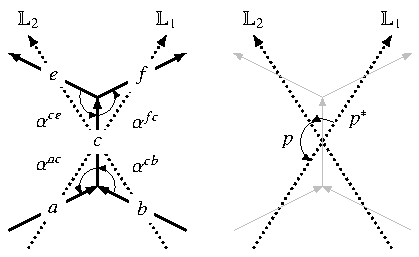
\includegraphics[width=0.56\textwidth]{figures/Fig_168_PDF276_Book264.pdf}
  \caption{两条闭曲线的局部交叉与相应角（原书 p.264）}\label{fig:band-intersection-local}
\end{figure}
于是
\[
  B_1=(a\oplus c\oplus f\oplus\cdots,\lambda_1^{ac}\alpha_{ac}+\lambda_1^{fc}\alpha_{fc}+\cdots),
\]
\[
  B_2=(b\oplus c\oplus e\oplus\cdots,\lambda_2^{cb}\alpha_{cb}+\lambda_2^{ce}\alpha_{ce}+\cdots),
\]
其中 $\alpha_{ac}$ 表示围绕公共标记点从 $c$ 指向 $a$ 的逆时针角。

\begin{lemma}{单个交点产生的带对象态射}{band-intersection-morphisms}
若两条曲线恰在一点 $p$ 相交，且 $B_1,B_2$ 是相应的一维局部系统带对象，则
\[
  \mathrm{topFuk}^{\pm}(B_1,B_2)=kp^*\oplus0,
  \qquad
  \mathrm{topFuk}^{\pm}(B_2,B_1)=0\oplus kp,
\]
其中 $p^*=1_c$，而 $p=\lambda_1^{ac}\alpha_{ac}-\lambda_2^{cb}\alpha_{cb}$。
\end{lemma}
\begin{proof}[证明思路]
仍假设所有标记点都在边界上。此时态射复形为
\[
  \mathrm{Hom}(B_1,B_2)=k1_c+k\alpha_{ba}+k\alpha_{ca}+k\alpha_{bc}+k\alpha_{ef}+k\alpha_{cf}+k\alpha_{ec},
\]
其微分为
\[
  x\longmapsto(\lambda_2^{cb}\alpha_{cb}+\lambda_2^{ce}\alpha_{ce})x
  -x(\lambda_1^{ac}\alpha_{ac}+\lambda_1^{fc}\alpha_{fc}).
\]
因此 $1_c$ 属于零次上同调；把它记为 $p$，因为它对应交点。容易验证，这就是唯一的上同调类。反向的态射空间中也有一个上同调类：$\lambda_1^{ac}\alpha_{ac}-\lambda_2^{cb}\alpha_{cb}$；也可以写成 $\lambda_1^{fc}\alpha_{fc}-\lambda_2^{ce}\alpha_{ce}$，因为两者之和是 $d1_c$。取前者记为 $p^*$，其次数为 $1$。\hfill$\square$
\end{proof}
% [Tutor Note: 证明把 $1_c$ 记作 $p$、把 $\lambda_1^{ac}\alpha_{ac}-\lambda_2^{cb}\alpha_{cb}$ 记作 $p^*$，与原书引理 9.24 的命名（$p^*=1_c$，$p=\lambda_1^{ac}\alpha_{ac}-\lambda_2^{cb}\alpha_{cb}$）正好相反；原书 p.264 亦如此。按下一引理的 $p\cdot p^*=\iota^*_{B_1}$ 与“后者次数为 $1$”，应以引理的命名为准，即 $1_c$ 是零次的 $p^*$。]

\begin{note}\label{note:multiple-band-intersections}
上述引理可以推广到有多个交点的曲线。每个交点都会在两个方向上各贡献一个态射，而态射的次数由两条曲线的定向决定。
\end{note}

\begin{lemma}{交点态射的乘积}{band-intersection-products}
若 $p$ 是两个带对象 $B_1,B_2$ 的交点，则
\[
  p\cdot p^*=\iota_{B_1}^*,\qquad p^*\cdot p=-\iota_{B_2}^*.
\]
\end{lemma}
\begin{proof}[证明思路]
这直接由 $\iota,\iota^*,p,p^*$ 的定义得到。\hfill$\square$
\end{proof}

现在设闭曲线 $L_1,\ldots,L_k$ 围成 $\dot S$ 中的一个多边形区域，并且存在弧系，使局部图形如下。把从 $L_{i+1}$ 到 $L_i$ 的次数 $1$ 态射记作 $p_i$，反方向的次数 $0$ 态射记作 $p_i^*$。
\begin{figure}[H]\centering
  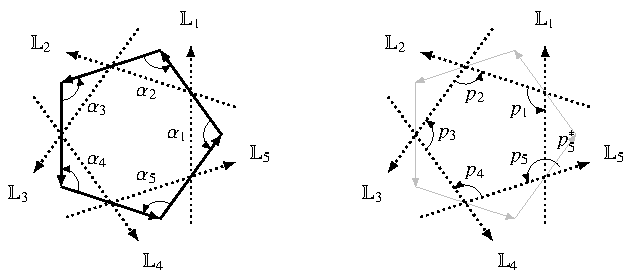
\includegraphics[width=0.66\textwidth]{figures/Fig_169_PDF277_Book265.pdf}
  \caption{由闭曲线围成的多边形区域（原书 p.265）}\label{fig:band-polygon-products}
\end{figure}

\begin{lemma}{多边形上的高阶乘积}{band-higher-product-polygon}
在上述情形中，
\[
  \mu(p_1,\ldots,p_{k-1})=c\,p_k^*,
  \qquad c=\lambda_1\cdots\lambda_k,
\]
其中 $c$ 是沿闭路的绕行变换。
\end{lemma}
\begin{proof}[证明思路]
每个 $p_i$ 的表达式形如 $\lambda_i\alpha_i+\cdots$，其中省略项是多边形外部的角，在计算中不起作用。带对象 $B(L_i,\lambda_i)$ 的扭曲微分也形如 $\lambda_i\alpha_i+\cdots$（以 $\lambda_i$ 表示角 $\alpha_i$ 上的系数）。计算 $\mu(p_1,\ldots,p_{k-1})$ 时，需要在各态射之间以所有可能方式插入 $\delta_i$ 并求和。唯一可能的非零乘积，是把 $\delta_k$ 插在末尾：
\[
  \mu(\lambda_1\alpha_1+\cdots,\ldots,\lambda_{k-1}\alpha_{k-1}+\cdots,
  \lambda_k\alpha_k+\cdots)=\lambda_1\cdots\lambda_k1_{a_k}.
\]
这是第 $k$ 条弧的恒等态射，对应于 $c p_k^*\in\mathrm{topFuk}^{\pm}(B_1,B_k)$。这项计算尚未在极小模型中进行；转入极小模型后结果仍然相同，因为其他可能贡献的树都会包含为零的乘积 $\mu_2(\alpha_i,\alpha_{i+1})$。\hfill$\square$
\end{proof}

与这个多边形对应的另一个乘积则依赖于所选的极小模型。为了在极小模型中计算乘积，对每个带对象 $B=(\bigoplus_i a_i,\lambda_i\alpha_i)$，需要选取分解
\[
  \mathrm{Hom}^{\bullet}(B,B)=I^{\bullet}\oplus H^{\bullet}\oplus R^{\bullet}.
\]
为此，选取一条弧 $a_m$ 和一个角 $\alpha_m$，称为标记弧和标记角。零次部分中，把除 $1_{a_m}$ 外的所有 $1_a$ 放入 $R^0$，并把 $1_B$ 放入 $H^0$；一次部分中，把 $\lambda_m\alpha_m$ 放入 $H^1$，并把所有 $\lambda_i\alpha_i-\lambda_{i+1}\alpha_{i+1}$ 放入 $I^1$。

\begin{lemma}{依赖标记弧的极小模型乘积}{minimal-model-polygon-product}
在上述情形中，
\[
  \mu(p_1,\ldots,p_{k-1},p_k)=c1_{L_k}\quad\text{或}\quad0.
\]
当且仅当 $L_k$ 的标记弧属于该多边形时，乘积取第一种情形。
\end{lemma}
\begin{proof}[证明思路]
此时唯一可能的非零乘积，是不插入任何 $\delta_i$ 的项：
\[
  \mu(\lambda_1\alpha_1+\cdots,\ldots,\lambda_k\alpha_k+\cdots)
  =\lambda_1\cdots\lambda_k1_{a_k}=c1_{a_k}.
\]
但 $1_{a_k}$ 不是 $\mathrm{Hom}(B(L_k,\lambda),B(L_k,\lambda))$ 中的上同调类，因此转到极小模型时须投影到上同调。该自同态空间中的零次上同调类为 $1_{L_k}=\sum_{a\in L_k}1_a$。由于除 $1_{a_m}$ 外的所有 $1_a$ 都被放在 $R$ 中，相应投影把它们映为零，并把 $1_{a_m}$ 映为 $1_{L_k}$。\hfill$\square$
\end{proof}

\begin{note}\label{note:geometric-fukaya-product}
这种现象与 Fukaya 范畴的几何构造相似。为了定义一条拉格朗日子流形与自身之间的态射空间，必须先选取一个变形。变形曲线与原曲线相交于两点，其中一点对应恒等态射。若这一点落在多边形边界上，就会有非零乘积；若落在多边形之外，则没有贡献。下图给出两种情形：
\begin{figure}[H]\centering
  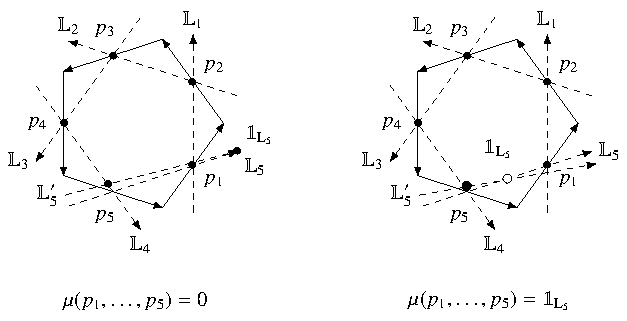
\includegraphics[width=0.89\textwidth]{figures/Fig_170_PDF279_Book267.pdf}
  \caption{多边形乘积的两种情形（原书 p.267）}\label{fig:polygon-products-two-cases}
\end{figure}
还需注意，上述乘积并非全部非零乘积。要完整计算所有乘积，技术上十分繁复，本书不再尝试。
\end{note}

由前述引理可知，带对象之间的态射由交点给出，而这些交点态射的乘积则通过计数由曲线围成的浸入圆盘得到。这正是我们对 Fukaya 型范畴所预期的行为。因此，可以把 $\mathrm{topFuk}^{\pm}(S,M)$ 看作 Fukaya 范畴的一种代数定义的替代模型。给定带标记曲面 $(S,M)$，可以构造一个带柱形端和 stop 的 Liouville 流形 $(X,\sigma)$：
\begin{enumerate}[label=(\roman*)]
  \item 在每个内部标记点周围切去一个圆盘。所得带边界曲面可赋予 Liouville 域 $X_0$ 的结构；
  \item 在由内部标记点产生的边界上粘接不带 stop 的圆柱；
  \item 对每个带有 $k$ 个标记点的边界分支，粘接带有 $k$ 个 stop 的圆柱。这些 stop 是终止在相邻标记点之间边界上的曲线。
\end{enumerate}

\begin{theorem}{拓扑 Fukaya 范畴与 partially wrapped Fukaya 范畴}{topological-partially-wrapped-equivalence}
带标记曲面 $(S,M)$ 的 Fukaya 范畴与 $(X,\sigma)$ 的 partially wrapped Fukaya 范畴 $A_\infty$ 等价：
\[
  \mathrm{topFuk}^{\pm}(S,M)\cong_\infty\mathrm{wrFuk}^{\pm}_{\sigma}X.
\]
\end{theorem}
\begin{proof}[证明思路]
在标记点附近把每条弧延伸到无穷远，可把它变成具有锥形端的拉格朗日子流形。在 partially wrapped Fukaya 范畴中，这些拉格朗日子流形之间的态射空间与 $\mathrm{topFuk}^{\pm}(S,M)$ 中弧之间的态射空间相同，因为每一次 Reeb 流动都对应一个角。两侧的高阶乘积也一致，因为浸入圆盘恰好对应于曲面 $S$ 上的多边形。最后，由于弧系把曲面剖分为多边形，可以应用定理\ref{thm:abouzaid-generation-criterion}中的生成判据，证明这些带锥形端的拉格朗日子流形生成 Fukaya 范畴。更多细节见文献\bookcite{36}的附录。\hfill$\square$
\end{proof}

在上述对应中，弦对象对应开拉格朗日子流形，带对象对应带局部系统的闭拉格朗日子流形。因此，可以把带标记曲面的（部分）wrapped Fukaya 范畴定义为由弦对象生成的范畴，而把正合 Fukaya 范畴定义为由带对象生成的子范畴：
\[
\begin{aligned}
  \mathrm{wrFuk}^{\pm}(S,M)&:=\langle S(L)\mid S(L)\text{ 是弦对象}\rangle
  =\mathrm{topFuk}^{\pm}(S,M),\\
  \mathrm{exFuk}^{\pm}(S,M)&:=\langle B(L,\lambda)\mid B(L,\lambda)\text{ 是带对象}\rangle
  \subset\mathrm{topFuk}^{\pm}(S,M).
\end{aligned}
\]

\begin{note}\label{note:exact-fukaya-spin-morse}
传统上，正合 Fukaya 范畴的对象是带有自旋结构和 Morse 函数的闭曲线\bookcite{218}。自旋结构用于确定符号；Morse 函数则用来定义 $L$ 的自同态，把曲线与其在该 Morse 函数下的 Hamilton 变形的交点视为态射。可以在曲线 $L$ 上标出三个特殊点 $\circ,*,\times$ 来表示这些数据。
\begin{itemize}
  \item $\circ$ 是 Morse 函数的极小点，对应 $\iota=1_L$。在本书的设定中，这等价于选择标记弧，并把 $\circ$ 放在标记弧之前；
  \item $*$ 是 Morse 函数的极大点，对应 $\iota^*=\lambda_m\alpha_m$。在本书的设定中，这等价于选择标记角，并把 $*$ 放在对应于 $\alpha_m$ 的线段中间；
  \item $\times$ 是自旋结构发生翻转的位置。在本书的术语中，带非平凡自旋结构的曲线具有绕行变换为 $-1$ 的局部系统。这可以通过令除一个以外的所有 $\lambda_i$ 都为 $1$，而剩余的一个取为 $-1$ 实现；把 $\times$ 放在这个取负号的角所对应的线段上。
\end{itemize}
\begin{figure}[H]\centering
  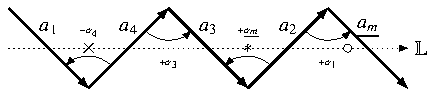
\includegraphics[width=0.64\textwidth]{figures/Fig_171_PDF280_Book268.pdf}
  \caption{带标记的弧、角与自旋翻转点（原书 p.268）}\label{fig:spin-morse-markers}
\end{figure}
\end{note}

\section{沿图粘合 Fukaya 范畴}\label{sec:gluing-categories}
\takeaway{沿带腿图粘合拓扑 Fukaya 范畴：带状图给出协变（余层）函子，管状图给出反变（层）函子，整体范畴是同伦（余）极限。圆柱的两个粘合例子分别把局部构件粘成 Kronecker 箭图与 $\mathbb P^1$ 的 $\mathbb Z_2$ 分次导出范畴。}
带标记曲面可以通过沿公共边粘合多边形构造；在 Fukaya 范畴层面也可以模拟这一过程。本节将讨论粘合 $A_\infty$ 范畴的几种方式。一般而言，粘合 $A_\infty$ 范畴或 dg 范畴需要用到高阶代数中的许多技巧，例如模型论\bookcite{239}及同伦（余）极限\bookcite{31,68}。这里仅在拓扑 Fukaya 范畴这一特殊情形中展示这些思想。一般框架的更多细节可参阅 Toen\bookcite{243,244}。

我们的目标是沿一种特定的一维空间粘合拓扑 Fukaya 范畴。此类空间由有限多个闭区间、半开区间和开区间组成，并将其中一些端点识别而得，称为带腿图 $\Gamma$。端点称为节点，区间称为边。根据区间的类型，边分为闭边、半开边和开边。半开边有时称为腿；开边不连接任何节点，有时称为孤立边。

图 $\Gamma$ 的每个具有有限多个连通分支的开子集，仍可视为带腿图。为排除具有无限多个连通分支的开集，我们将 $\mathrm{Open}(\Gamma)$ 定义为由所有有限多个连通分支的开集组成的范畴，态射为包含映射。若两个这样的开集 $\Upsilon_1,\Upsilon_2$ 的交为 $\Upsilon_{12}:=\Upsilon_1\cap\Upsilon_2$，则在 $\mathrm{Open}(\Gamma)$ 中有粘合图：
\begin{figure}[H]\centering
  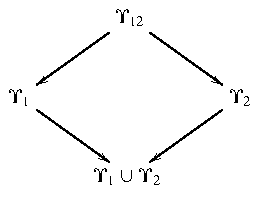
\includegraphics[width=0.35\textwidth]{figures/Fig_172_PDF281_Book269.pdf}
  \caption{开覆盖的粘合图式（原书 p.269）}\label{fig:open-cover-gluing-diagram}
\end{figure}
范畴论地说，$\Upsilon_1\cup\Upsilon_2$ 是图式 $\Upsilon_1\leftarrow\Upsilon_{12}\to\Upsilon_2$ 的余极限，因为任何补全该图式的方式都唯一地经由它分解。

\subsection*{沿带状图\index{daizhuangtu@带状图|hyperpage}粘合}
\begin{definition}{弧系的带状图}{ribbon-graph}
设 $A$ 是带标记曲面 $(S,M)$ 的生成弧系，并假设所有边界段都属于 $A$。带状图 $\Gamma_A$ 是一个带腿图：每个多边形中心对应一个节点；每条内部弧对应一条闭边；每条边界弧对应一条半开边。各边连接到弧所围多边形对应的节点。\footnote{之所以称为带状图，是因为它在 $(S,M)$ 中的自然嵌入允许我们把边加粗为带。}

对每个开集 $\Upsilon\in\mathrm{Open}(\Gamma_A)$，可以构造一个新的带标记曲面 $(S_\Upsilon,M_\Upsilon)$：把子图中各节点对应的多边形，沿 $\Upsilon$ 中闭边所对应的弧粘在一起。若 $\Upsilon$ 中含有孤立边，则为每条孤立边添加一个带两个标记点的圆盘。多边形的角就是 $S_\Upsilon$ 的标记点。
\end{definition}

\begin{theorem}{带状图上的协变范畴值函子}{ribbon-graph-cosheaf-functor}
存在一个协变函子，从范畴 $\mathrm{Open}(\Gamma_A)$ 出发，取值于以 $A_\infty$ 函子为态射的导出 $A_\infty$ 范畴所构成的范畴，并将每个 $\Upsilon$ 映到 $(S_\Upsilon,M_\Upsilon)$ 的拓扑 Fukaya 范畴：
\[
  R\colon\mathrm{Open}(\Gamma_A)\longrightarrow\mathrm{DCAT}_\infty,
  \qquad \Upsilon\longmapsto\mathrm{topFuk}^{\pm}(S_\Upsilon,M_\Upsilon).
\]
\end{theorem}
\begin{proof}[证明思路]
设 $\phi\colon\Upsilon_1\to\Upsilon_2$ 是 $\mathrm{Open}(\Gamma_A)$ 中的态射。对 $(S_{\Upsilon_i},M_{\Upsilon_i})$，取由各多边形边组成的弧系 $A_i$。态射 $\phi$ 诱导弧系之间的映射 $A_1\to A_2$，因为 $\Upsilon_1$ 中的每条边都落在 $\Upsilon_2$ 中唯一一条边上。这一映射未必是单射：$A_1$ 中两条弧可能映到 $A_2$ 中同一条弧。

每个非平凡角都唯一对应于一个多边形及两条入弧（对偶地，对应于一个节点及两条边），所以 $\phi$ 也诱导角之间的映射，从而得到 gentle 代数态射
\[
  F\colon\mathrm{Gtl}^{\pm}A_1\longrightarrow\mathrm{Gtl}^{\pm}A_2.
\]
这个态射保持 $A_\infty$ 结构：若某个角同时出现在两个曲面中，就表示相应多边形也同时出现在两者中。因此，在 $S_{\Upsilon_2}$ 中的任意多边形浸入也会出现在 $S_{\Upsilon_1}$ 中。转到导出范畴后得到严格的 $A_\infty$ 函子
\[
  R(\Upsilon_i):=D\mathrm{Gtl}^{\pm}A_i,
  \qquad R(\phi):=DF\colon R(\Upsilon_1)\longrightarrow R(\Upsilon_2).
\]
复合律由构造直接得到。\hfill$\square$
\end{proof}

函子 $R$ 很像一个预层，只是它由协变函子而非反变函子定义；换言之，它是一个余预层。甚至可以把 $R$ 称为 $A_\infty$ 范畴的余层。这表示，正如层的整体截面可以由局部截面沿交集相容地粘合而成，范畴 $R(\Upsilon_1\cup\Upsilon_2)$ 也是如下图式的一个普适构造：
\begin{figure}[H]\centering
  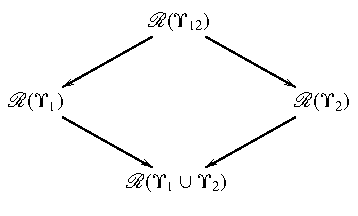
\includegraphics[width=0.45\textwidth]{figures/Fig_173_PDF283_Book271.pdf}
  \caption{范畴余层的粘合图式（原书 p.271）}\label{fig:categorical-cosheaf-diagram}
\end{figure}
数学上，$R(\Upsilon_1\cup\Upsilon_2)$ 是图式 $R(\Upsilon_1)\leftarrow R(\Upsilon_{12})\to R(\Upsilon_2)$ 的同伦余极限\index{tonglunyujixian@同伦余极限|hyperpage}。这是范畴中经典余极限的高阶版本，并且与拟同构和扭曲完备化相容。其精确定义超出本书范围；更多信息见 Haiden、Katzarkov 和 Kontsevich\bookcite{115}，Dyckerhoff 和 Kapranov\bookcite{65}，Sibilla、Treumann 和 Zaslow\bookcite{232}，Nadler\bookcite{189,188,191}，Pascaleff 和 Sibilla\bookcite{204}。

\begin{example}[由两个三角形粘合成圆柱]\label{ex:cylinder-ribbon-gluing}
可以把两个边界各有一个标记点的圆柱看成两个三角形沿边粘合而成：
\begin{figure}[H]\centering
  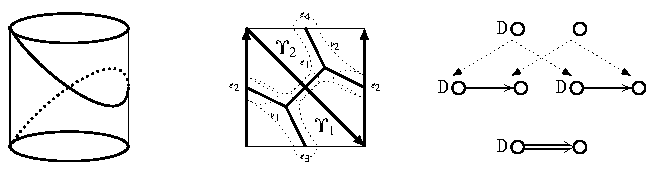
\includegraphics[width=0.86\textwidth]{figures/Fig_174_PDF283_Book271.pdf}
  \caption{圆柱的带状图及相应的箭图粘合（原书 p.271）}\label{fig:cylinder-ribbon-gluing}
\end{figure}
带状图有两个三价节点 $v_1,v_2$，由两条边 $e_1,e_2$ 相连；另有两条开边 $e_3,e_4$，分别连到 $v_1,v_2$。取开覆盖
\[
\begin{aligned}
  \Upsilon_1&=\{v_1\}\cup\operatorname{Int}(e_1)\cup\operatorname{Int}(e_2)\cup\operatorname{Int}(e_3),\\
  \Upsilon_2&=\{v_2\}\cup\operatorname{Int}(e_1)\cup\operatorname{Int}(e_2)\cup\operatorname{Int}(e_4),\\
  \Upsilon_{12}&=\operatorname{Int}(e_1)\cup\operatorname{Int}(e_2),
\end{aligned}
\]
则 Fukaya 范畴图式由两个线性箭图的导出范畴构成，二者都包含一个只有两个顶点、没有箭的箭图的导出范畴。其同伦余极限是沿这两个顶点粘合两个线性箭图所得的导出范畴，也就是 Kronecker 箭图的导出范畴。
\end{example}

\begin{note}\label{note:ribbon-graph-skeleton}
利用带状图粘合 Fukaya 范畴，是 Kontsevich 关于某些非紧辛流形的 wrapped Fukaya 范畴应由拉格朗日骨架\index{lagelangrigujia@拉格朗日骨架|hyperpage}构造这一思想的一维实现。拉格朗日骨架是辛流形的一个（可能奇异的）形变收缩核。它在骨架上给出一个范畴余层，相应的同伦余极限就是辛流形的 wrapped Fukaya 范畴。考察骨架的组合结构，便可把 wrapped Fukaya 范畴视为若干简单 $A_\infty$ 范畴的余极限。在这里，带状图就是拉格朗日骨架；简单部分对应于图节点的邻域（给出线性箭图 $L_n$ 的模范畴导出范畴 $D\mathrm{mod}^{\pm}L_n$）和边的邻域（给出 $\mathbb C$ 的导出范畴）。
\end{note}

\subsection*{沿管状图\index{guanzhuangtu@管状图|hyperpage}粘合}
\begin{definition}{切曲线与管状图}{tubular-graph}
设 $(S,M)$ 是带标记曲面。简单闭曲线是圆周 $S^1$ 到 $S$ 的一个嵌入，并且不与围绕某个内部标记点的小圆同伦。切集\index{qieji@切集|hyperpage} $C$ 是一组两两不相交且彼此不同伦的简单闭曲线。

由切集 $C$ 可构造一个带腿图，称为管状图 $\Gamma_C$。它的节点是删去这些简单闭曲线后所得的连通分支，边则对应简单闭曲线和内部标记点。对应简单闭曲线的边连接到该曲线围出的各连通分支所对应节点。其他边可视为半开边，因为它们只连接到包含相应标记点的节点。

与带状图情形相同，对每个开集 $\Upsilon\in\mathrm{Open}(\Gamma_C)$，都可构造一个新的带标记曲面：把 $\Upsilon$ 中节点对应的连通分支，沿其闭边所对应的闭曲线粘合；每条开边添加一个圆柱，并把未与内部标记点粘合的开端收缩。\footnote{在把标记点本身视为标记边界分支的形式体系中，最后一步并不需要，见第~\ref{note:marked-surface-conventions}~节的注记。}记所得曲面为 $(S_\Upsilon,M_\Upsilon)$。
\end{definition}

\begin{theorem}{管状图上的反变范畴值函子}{tubular-graph-sheaf-functor}
存在一个从范畴 $\mathrm{Open}(\Gamma_C)$ 到由导出 $A_\infty$ 范畴组成的范畴的反变函子；后者的态射为 $A_\infty$ 函子。该函子将每个 $\Upsilon$ 映到 $(S_\Upsilon,M_\Upsilon)$ 的拓扑 Fukaya 范畴：
\[
  T\colon\mathrm{Open}(\Gamma_C)^{\mathrm{op}}\longrightarrow\mathrm{DCAT}_\infty,
  \qquad \Upsilon\longmapsto\mathrm{topFuk}^{\pm}(S_\Upsilon,M_\Upsilon).
\]
\end{theorem}
\begin{proof}[证明思路]
取一个生成 $(S,M)$ 的弧系 $A$。给定 $\Upsilon\in\mathrm{Open}(\Gamma_C)$，每条弧 $a$ 都交替分解为位于 $(S_\Upsilon,M_\Upsilon)$ 内的弧段 $a_i$ 和不在其中的弧段 $b_i$。某些 $a_i$ 在 $(S_\Upsilon,M_\Upsilon)$ 中可能彼此同位变形，但它们合在一起仍能剖分 $S_\Upsilon$。将这组弧记为 $A_\Upsilon$，并令 $T(\Upsilon):=D\mathrm{Gtl}^{\pm}A_\Upsilon$。

若 $\phi\colon\Upsilon_1\to\Upsilon_2$ 是 $\mathrm{Open}(\Gamma_C)$ 中的态射，则 $A_{\Upsilon_2}$ 中每条弧 $a$ 都分解为若干子弧 $a_i$。映射
\[
  T\colon\mathrm{Gtl}^{\pm}A_{\Upsilon_2}\longrightarrow D\mathrm{Gtl}^{\pm}A_{\Upsilon_1},
  \qquad a\longmapsto\bigoplus_{a_i\subset a}a_i
\]
可以扩展为 $A_\infty$ 态射。若角 $\alpha$ 同时出现在 $S_{\Upsilon_2}$ 与 $S_{\Upsilon_1}$ 中，就令 $T(\alpha)=\alpha$，并把后者看成 $T(h(a))$ 与 $T(t(a))$ 的相应直和项之间的映射；若角 $\alpha$ 不出现在 $S_{\Upsilon_1}$ 中，则令 $T(\alpha)=0$。

考察 $A_{\Upsilon_1}$ 中弧之间的角，可见它们分成两类：一类也存在于 $S_{\Upsilon_2}$ 中，另一类是收缩闭曲线后新产生的角。后者可看成 $S_{\Upsilon_2}$ 中弧之间的弦。若 $S_{\Upsilon_2}\setminus S_{\Upsilon_1}$ 中的角序列 $a_0\leftarrow\cdots\leftarrow a_k$ 与一条弦 $\beta$ 围成浸入多边形，就令高阶分量 $T(\alpha_1,\ldots,\alpha_k)=\pm\beta$：
\begin{figure}[H]\centering
  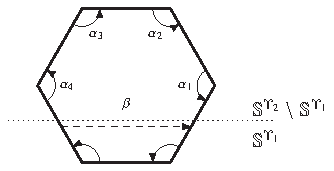
\includegraphics[width=0.44\textwidth]{figures/Fig_175_PDF285_Book273.pdf}
  \caption{收缩闭曲线后出现的高阶分量（原书 p.273）}\label{fig:tubular-gluing-higher-map}
\end{figure}
容易验证，这一赋值使 $T$ 成为 $A_\infty$ 态射。转到导出范畴后得到函子
\[
  T(\Upsilon_i):=D\mathrm{Gtl}^{\pm}A_i,
  \qquad T(\phi):=DT\colon T(\Upsilon_2)\longrightarrow T(\Upsilon_1).
\]
复合律由构造直接得到。\hfill$\square$
\end{proof}

\begin{note}\label{note:tubular-gluing-limit}
与带状图的情形相同，这个 $A_\infty$ 函子可以看成一个层，而范畴 $T(\Upsilon_1\cup\Upsilon_2)$ 可由图式
\[
T(\Upsilon_1)\longrightarrow T(\Upsilon_1\cap\Upsilon_2)\longleftarrow T(\Upsilon_2)
\]
通过同伦极限\index{tonglunjixian@同伦极限|hyperpage}构造。为使这一构造正常工作，必须对 Fukaya 范畴取 ind-完备化\footnote{例如，若 $\mathrm{topFuk}^{\pm}(\dot S)=D\mathrm{Mod}^{\pm}Q$，其 ind-完备化为 $D\mathrm{MOD}^{\pm}Q$。}。更多信息见 Pascaleff 和 Sibilla\bookcite{204}。请注意，由于采用了不同约定，他们把这种粘合称为沿闭子图粘合。
\end{note}

\begin{example}[沿闭曲线切开圆柱]\label{ex:cylinder-tubular-gluing}
仍考虑两个边界分支各有一个标记点的圆柱，并取一条把圆柱切成两半的简单闭曲线：
\begin{figure}[H]\centering
  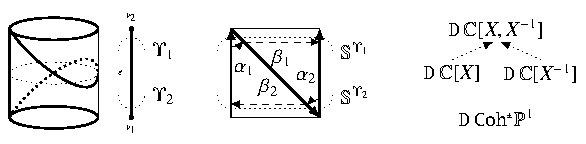
\includegraphics[width=0.94\textwidth]{figures/Fig_176_PDF286_Book274.pdf}
  \caption{圆柱切分、角及相应的代数图式（原书 p.274）}\label{fig:cylinder-tubular-gluing}
\end{figure}
管状图有两个一价节点 $v_1,v_2$，由一条边 $e$ 相连。每个节点对应一个边界上有一个标记点的穿孔圆盘，二者的交集是带有两个内部标记点的球面。取开覆盖
\[
  \Upsilon_1=v_1\cup\operatorname{Int}(e),\qquad
  \Upsilon_2=v_2\cup\operatorname{Int}(e),\qquad
  \Upsilon_{12}=\operatorname{Int}(e),
\]
则曲面 $S_{\Upsilon_1}$、$S_{\Upsilon_2}$ 都是边界上有一个标记点、内部有一个标记点的圆盘，而 $S_{\Upsilon_1\cap\Upsilon_2}$ 是开圆柱（或带两个标记点的球面）。

若取与例\ref{ex:cylinder-ribbon-gluing}相同的弧系，弧集 $\{a_1,a_2\}$ 在这三个曲面上都限制为两条弧。除原有角 $\alpha_1,\alpha_2\colon a_1\to a_2$ 外，交集曲面中还多出两个角 $\beta_1,\beta_2\colon a_2\to a_1$。角 $\beta_1$ 出现在 $S_{\Upsilon_2}$ 中，但不出现在 $S_{\Upsilon_1}$ 中；对 $\beta_2$ 则相反。相应的 gentle 代数由下列关系描述：
\[
\begin{aligned}
  \mathrm{Gtl}^{\pm}A_1&=\mathbb C\langle a_1,a_2,\alpha_1,\alpha_2,\beta_2\rangle
  /(\alpha_1\beta_2-1_{a_2},\,\beta_2\alpha_1-1_{a_1}),\\
  \mathrm{Gtl}^{\pm}A_2&=\mathbb C\langle a_1,a_2,\alpha_1,\alpha_2,\beta_1\rangle
  /(\alpha_2\beta_1-1_{a_2},\,\beta_1\alpha_2-1_{a_1}),\\
  \mathrm{Gtl}^{\pm}A_{12}&=\mathbb C\langle a_1,a_2,\alpha_1,\alpha_2,\beta_1,\beta_2\rangle
  /(\alpha_1\beta_2-1_{a_2},\,\beta_2\alpha_1-1_{a_1},\\
  &\hspace{39mm}\alpha_2\beta_1-1_{a_2},\,\beta_1\alpha_2-1_{a_1}).
\end{aligned}
\]

% [Tutor Note: 原书 p.274 把 $\mathrm{Gtl}^{\pm}A_2$ 的第二条关系印作 $\beta_1\alpha_1-1_{a_1}$，但 $\alpha_2$ 与 $\beta_1$ 才互为逆：$\alpha_2\beta_1=1_{a_2}$ 必须配 $\beta_1\alpha_2=1_{a_1}$。译文按后者写作 $\beta_1\alpha_2$；若沿用 $\beta_1\alpha_1$，该代数不会 Morita 等价于 $\mathbb C[\alpha_1\beta_1]$。]
由此得到相应的导出范畴粘合图式：
\begin{figure}[H]\centering
  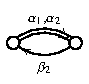
\includegraphics[width=0.9\textwidth]{figures/Fig_177_PDF286_Book274.pdf}
  \caption{两个区域中的第一组角关系（原书 p.274）}\label{fig:cylinder-tubular-algebra-one}
\end{figure}
\begin{figure}[H]\centering
  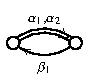
\includegraphics[width=0.9\textwidth]{figures/Fig_178_PDF286_Book274.pdf}
  \caption{两个区域中的第二组角关系（原书 p.274）}\label{fig:cylinder-tubular-algebra-two}
\end{figure}
\begin{figure}[H]\centering
  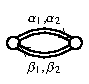
\includegraphics[width=0.9\textwidth]{figures/Fig_179_PDF286_Book274.pdf}
  \caption{交集曲面上的两组角关系（原书 p.274）}\label{fig:cylinder-tubular-algebra-intersection}
\end{figure}
因此，$\mathrm{Gtl}^{\pm}A_1$ 与 $\mathbb C[\alpha_2\beta_2]=\mathbb C[X]$ Morita 等价，$\mathrm{Gtl}^{\pm}A_2$ 与 $\mathbb C[\alpha_1\beta_1]=\mathbb C[Y]$ Morita 等价。最后，在 $\mathrm{Gtl}^{\pm}A_{12}$ 中，$\alpha_1\beta_1$ 与 $\beta_2\alpha_2$ 互为逆元，所以该代数与 $\mathbb C[X,Y]/(XY-1)$ Morita 等价。

这说明我们正在把 $\mathbb C[X]$ 与 $\mathbb C[X^{-1}]$ 的导出范畴沿 $\mathbb C[X,X^{-1}]$ 的导出范畴粘合。所得同伦极限是两条仿射直线沿 $\mathbb C^*$ 粘合后的导出范畴，换言之，就是 $\mathbb P^1$ 的 $\mathbb Z_2$ 分次导出范畴。
\end{example}

\section{粘合与镜像对称}\label{sec:gluing-mirror-symmetry}
\takeaway{裤子曲面 $(S^2,\{0,1,\infty\})$ 的拓扑 Fukaya 范畴等价于矩阵分解范畴 $\mathrm{MF}^{\pm}(\mathbb C^3,XYZ)$；用矩阵分解的 Čech 型粘合把裤子拼成高亏格曲面，得到非仿射 Landau--Ginzburg 模型，两侧图式的同伦极限互相对应。}
现在用上一节的粘合方法研究穿孔黎曼曲面的镜像对称。基本思路是先构造一个镜像对称的基本构件，再把多个这样的构件粘合起来。基本构件是裤子曲面\index{kuziqumian@裤子曲面|hyperpage}，也就是有三个标记点的球面\index{daisangebiaojidiandeqiumian@带三个标记点的球面|hyperpage} $(S^2,\{0,1,\infty\})$。其镜像对称由 Abouzaid、Auroux、Efimov、Katzarkov 和 Orlov\bookcite{1}建立。

\begin{theorem}{裤子曲面的镜像对称}{pants-mirror-equivalence}
裤子曲面的拓扑 Fukaya 范畴与 Landau--Ginzburg 模型 $(\mathbb C^3,XYZ)$ 的矩阵分解范畴导出等价：
\[
  \mathrm{topFuk}^{\pm}(S^2,\{0,1,\infty\})
  \cong_\infty \mathrm{MF}^{\pm}(\mathbb C^3,XYZ).
\]
\end{theorem}
\begin{proof}[证明思路]
把球面剖分成两个三角形，得到由三条弧 $\{x,y,z\}$ 组成的弧系。下图给出相应的曲面、三角剖分和箭图：
\begin{figure}[H]\centering
  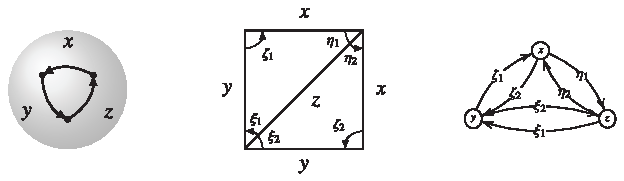
\includegraphics[width=0.91\textwidth]{figures/Fig_180_PDF287_Book275.pdf}
  \caption{裤子曲面的弧系、三角剖分及其箭图（原书 p.275）}\label{fig:pants-arcs-quiver}
\end{figure}
所有箭的次数都是 $1$，例如
\[
\begin{aligned}
  \mu(\zeta_1,\xi_1,\eta_1)=\mu(\eta_2,\xi_2,\zeta_2)&=1_x,\\
  \mu(\xi_1,\eta_1,\zeta_1)=\mu(\zeta_2,\eta_2,\xi_2)&=1_y,\\
  \mu(\eta_1,\zeta_1,\xi_1)=\mu(\xi_2,\zeta_2,\eta_2)&=1_z.
\end{aligned}
\]
$B$ 侧有三个显然的矩阵分解。令 $R=\mathbb C[X,Y,Z]$，则
\[
  M_X=\left(R^{\oplus2},\begin{pmatrix}0&X\\YZ&0\end{pmatrix}\right),\quad
  M_Y=\left(R^{\oplus2},\begin{pmatrix}0&Y\\XZ&0\end{pmatrix}\right),\quad
  M_Z=\left(R^{\oplus2},\begin{pmatrix}0&Z\\XY&0\end{pmatrix}\right).
\]
从 $M_Z$ 到 $M_Y$ 的 Hom 空间是 $\mathrm{Mat}_{2\times2}(R)$，其微分为
\[
  d\begin{pmatrix}a&b\\c&d\end{pmatrix}
  =\begin{pmatrix}0&Y\\XZ&0\end{pmatrix}\begin{pmatrix}a&b\\c&d\end{pmatrix}
   -\begin{pmatrix}a&-b\\-c&d\end{pmatrix}\begin{pmatrix}0&Z\\XY&0\end{pmatrix}
  =\begin{pmatrix}Yc+bXY&Yd-aZ\\XZa-dXY&XZb+cZ\end{pmatrix}.
\]
该空间的上同调为 $\mathbb C[X]\xi_1$，其中
\[
  \xi_1=\begin{pmatrix}0&-1\\X&0\end{pmatrix}.
\]
类似计算给出下表（表中非对角项表示由相应矩阵生成的多项式模）：
{\small
\[
\begin{array}{c|ccc}
  &M_X&M_Y&M_Z\\\hline
M_X&\mathbb C[Y]1+\mathbb C[Z]1
&\mathbb C[Z]\!\begin{pmatrix}0&-1\\Z&0\end{pmatrix}
&\mathbb C[Y]\!\begin{pmatrix}0&-1\\Y&0\end{pmatrix}\\[5pt]
M_Y&\mathbb C[Z]\!\begin{pmatrix}0&-1\\Z&0\end{pmatrix}
&\mathbb C[Z]1+\mathbb C[X]1
&\mathbb C[X]\!\begin{pmatrix}0&-1\\X&0\end{pmatrix}\\[5pt]
M_Z&\mathbb C[Y]\!\begin{pmatrix}0&-1\\Y&0\end{pmatrix}
&\mathbb C[X]\!\begin{pmatrix}0&-1\\X&0\end{pmatrix}
&\mathbb C[X]1+\mathbb C[Y]1
\end{array}
\]
}
根据矩阵中出现的变量，把六个次数为 $1$ 的生成元记为 $\xi_1,\xi_2,\ldots,\zeta_1,\zeta_2$。只有希腊字母相同的乘积非零。例如
\[
  \zeta_1\eta_1=
  \begin{pmatrix}0&-1\\Z&0\end{pmatrix}
  \begin{pmatrix}0&-1\\Y&0\end{pmatrix}
  =\begin{pmatrix}-Y&0\\0&-Z\end{pmatrix}
  =d\begin{pmatrix}0&0\\1&0\end{pmatrix}.
\]
所以这六个次数为 $1$ 的态射的行为恰好与上述弧系中的角相同。令 $M=M_X\oplus M_Y\oplus M_Z$，便有
\[
  \mathrm{MF}^{\pm}(M,M)\cong\mathrm{Gtl}^{\pm}A.
\]
这个代数同构可提升为 $A_\infty$ 同构。例如，为验证 $\mu(\zeta_1,\xi_1,\eta_1)=1_{M_X}$，取分解使
\[
  \begin{pmatrix}0&0\\0&1\end{pmatrix}\in R,
  \qquad
  \begin{pmatrix}-X&0\\0&-Y\end{pmatrix}
  =d\begin{pmatrix}0&0\\-1&0\end{pmatrix}\in I.
\]
于是
\[
\begin{aligned}
  \mu(\zeta_1,\xi_1,\eta_1)
  &=\pi\begin{pmatrix}0&-1\\Z&0\end{pmatrix}
    h\!\left(\begin{pmatrix}0&-1\\Y&0\end{pmatrix}
             \begin{pmatrix}0&-1\\X&0\end{pmatrix}\right)
   +\pi h\!\left(\begin{pmatrix}0&-1\\Z&0\end{pmatrix}
             \begin{pmatrix}0&-1\\Y&0\end{pmatrix}\right)
             \begin{pmatrix}0&-1\\X&0\end{pmatrix}\\
  &=\pi\begin{pmatrix}0&-1\\Z&0\end{pmatrix}
    h\begin{pmatrix}-X&0\\0&-Y\end{pmatrix}
   +\pi h\begin{pmatrix}-Y&0\\0&-Z\end{pmatrix}
             \begin{pmatrix}0&-1\\X&0\end{pmatrix}\\
  &=\pi\begin{pmatrix}0&-1\\Z&0\end{pmatrix}
    \begin{pmatrix}0&0\\-1&0\end{pmatrix}
   +\pi\begin{pmatrix}0&0\\-1&0\end{pmatrix}
             \begin{pmatrix}0&-1\\X&0\end{pmatrix}\\
  &=\pi\begin{pmatrix}1&0\\0&0\end{pmatrix}
   +\pi\begin{pmatrix}0&0\\0&1\end{pmatrix}=1_{M_X}.
\end{aligned}
\]
% [Tutor Note: 原书 p.276 这一推导的末行印作 $=-\,\mathbb{1}$，与所要证的 $\mu(\zeta_1,\xi_1,\eta_1)=1_{M_X}$ 矛盾；译文取 $1_{M_X}$。若按原书取 $-1$，则须同步改变 $\mu(\zeta_1,\xi_1,\eta_1)=1_x$ 的符号约定，属原书笔误。]
与其逐一检查所有非零高阶乘积，不如证明 $\mu(\zeta_1,\xi_1,\eta_1)$ 和 $\mu(\eta_2,\xi_2,\zeta_2)$ 的取值唯一确定代数 $\mathrm{Gtl}^{\pm}A$ 上的 $A_\infty$ 结构（至 $A_\infty$ 同构）。这可以用 $A_\infty$ 代数的变形理论和 Hochschild 上同调证明；第\ref{ch:deformation}章，尤其是定理\ref{thm:ainfty-deformation-classification}，将更详细地说明这一点。

证明的最后一步是说明这三个矩阵分解生成 $\mathrm{MF}^{\pm}(\mathbb C^3,XYZ)$。由定理\ref{thm:buchweitz-singularity-category}，矩阵分解范畴等价于 $X=W^{-1}(0)$ 的奇点范畴；$X$ 由三个坐标平面组成。在这一对应下，$M_X[1]$ 对应于 $R/(X)$，即 $YZ$ 平面的结构层。由于 $YZ$ 平面光滑，其结构层生成该平面的导出范畴。在 $D^b\mathrm{Coh}X$ 中，$R/(X)$ 生成所有支撑在 $YZ$ 平面上的层。因此，$D^b\mathrm{Coh}X$ 由 $R/(X),R/(Y),R/(Z)$ 生成，奇点范畴也由这些对象生成。证明的更多细节见\bookcite{1,155}。\hfill$\square$
\end{proof}

\begin{note}\label{note:pants-singularity-mirror}
矩阵分解范畴描述了 $\mathbb C^3$ 中 $XYZ=0$ 的奇点集。这个奇点集由三条在原点相接的仿射直线组成。对奇点集上的每一点，都可以为该点的点层构造局部自由分解，并考察其二周期尾部，从而得到矩阵分解。对 $p=(0,0,z)$，所得矩阵分解为
\[
  M_p=\left(\begin{array}{cccc}
  0&X&0&0\\YZ&0&0&0\\Z-z&0&0&X\\0&z-Z&YZ&0
  \end{array}\right)=\operatorname{Cone}(\zeta_1\ \ \zeta_2-z).
\]
它对应于裤子曲面上绕某个标记点的圆周 $L_p$，并带有绕行变换为 $z$ 的局部系统。

对原点，得到矩阵分解 $R\otimes\Lambda_3$，其微分为
\[
  d\phi:=\iota_X\phi+\iota_Y\phi+\iota_Z\phi
  +(YZ\,dX+XZ\,dY+XY\,dZ)\wedge\phi.
\]
该矩阵分解与下列对象拟同构：
\[
  M_0=\operatorname{Cone}\!\left(
  M_x\oplus M_y\oplus M_z\xrightarrow{\ \xi_1\pm\cdots\pm\zeta_2\ }
  M_x\oplus M_y\oplus M_z\right).
\]
它对应于一条环绕裤子曲面“裆部”的曲线 $L_0$，其局部系统的绕行变换为 $\lambda=-1$。\footnote{文献\bookcite{71,220}中通过非平凡自旋结构实现这一局部系统。}

最后，三个矩阵分解 $M_X,M_Y,M_Z$ 分别对应于支撑在三条仿射直线中两条上的对象。注意，$p=(0,0,z)$ 处的 $M_p$ 可以看成 $M_X$ 或 $M_Y$ 上的锥，却不能看成 $M_Z$ 上的锥。因此，$p$ 属于 $M_X,M_Y$ 的支撑，而不属于 $M_Z$ 的支撑。从 $A$ 侧看这一点也很清楚：$L_p$ 与弧 $x,y$ 相交，但不与 $z$ 相交。
\begin{figure}[H]\centering
  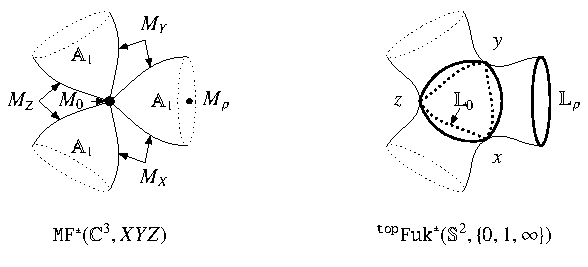
\includegraphics[width=0.93\textwidth]{figures/Fig_181_PDF290_Book278.pdf}
  \caption{裤子曲面上的矩阵分解与曲线对象（原书 p.278）}\label{fig:pants-singularity-objects}
\end{figure}
\end{note}

这个镜像对应也与粘合相容。下面说明如何把不同的裤子曲面粘在一起，从而为亏格较高、标记点较多的曲线构造非仿射 Landau--Ginzburg 模型。

\begin{example}[粘合裤子曲面得到四标记球面的镜像]\label{ex:gluing-pants-landau-ginzburg}
取 $U_1,U_2\cong\mathbb C^3$，其中 $U_i=V(R_i)$，$R_i=\mathbb C[X_i,Y_i,Z_i]$。要把这两个仿射空间粘起来，可取一个过渡映射，使 $X_1Y_1Z_1$ 与 $X_2Y_2Z_2$ 对应，并把其中一个坐标取逆。例如
\[
  X_2=X_1Z_1,\qquad Y_2=Y_1Z_1,\qquad Z_2=Z_1^{-1}.
\]
交集 $U_{12}$ 是环
\[
  R_{12}=\mathbb C[X_1,Y_1,Z_1^{\pm1}]
  =\mathbb C[X_2,Y_2,Z_2^{\pm1}]
\]
所对应的簇，且该环含有函数 $\ell=X_1Y_1Z_1=X_2Y_2Z_2$。

嵌入 $U_{12}\hookrightarrow U_i$ 诱导限制函子
\[
  \mathrm{MF}^{\pm}(R_i,\ell)\longrightarrow\mathrm{MF}^{\pm}(R_{12},\ell),
  \qquad (M,d)\longmapsto(M\otimes_{R_i}R_{12},d\otimes_{R_i}1).
\]
若把矩阵分解 $M_X,M_Y,M_Z$ 限制到交集，会发生什么？把 $Z$ 取逆后，态射 $\zeta_1,\zeta_2$ 变成可逆态射，矩阵分解 $M_Z$ 成为零对象，因为
\[
  1_{M_Z}=
  \begin{pmatrix}0&Z\\XY&0\end{pmatrix}
  \begin{pmatrix}0&0\\Z^{-1}&0\end{pmatrix}
  +\begin{pmatrix}0&0\\Z^{-1}&0\end{pmatrix}
  \begin{pmatrix}0&Z\\XY&0\end{pmatrix}
  =d\begin{pmatrix}0&0\\Z^{-1}&0\end{pmatrix}.
\]
因此，在 $\mathrm{MF}^{\pm}(R_{12},\ell)$ 中，$M_X\cong M_Y[1]$ 且 $M_Z=0$。此外，$M_X$ 的自同态环为 $\mathbb C[Z,Z^{-1}]1_{M_X}$，所以
\[
  \mathrm{MF}^{\pm}(\mathbb C[X,Y,Z,Z^{-1}],XYZ)
  \cong_\infty D\mathbb C[Z,Z^{-1}],
\]
它也就是两个标记点的球面的 Fukaya 范畴。若沿 $U_{12}$ 把 $U_1$ 与 $U_2$ 粘起来，就得到一个簇 $X$，其全局函数为 $\ell=X_1Y_1Z_1=X_2Y_2Z_2$；这就是一个非仿射 Landau--Ginzburg 模型。

范畴 $\mathrm{MF}^{\pm}(X,\ell)$ 的对象是二元组 $(P,d)$，其中 $P$ 是 $\mathbb Z_2$ 分次局部自由层，且 $d\in\mathrm{Hom}(P,P)$ 满足 $d^2=\ell$。局部自由层由三元组 $(R_1^n,R_2^n,U)$ 确定，其中 $U\in\mathrm{Mat}_{n\times n}(R_{12})$ 可逆。微分由一对映射 $d_1,d_2$ 给出，满足
\[
  (d_1^2,d_2^2)=(X_1Y_1Z_1,X_2Y_2Z_2),\qquad d_1=Ud_2U^{-1}
\]
（后一等式在 $R_{12}$ 上成立）。由此可以构造四个矩阵分解：
{\scriptsize
\[
\begin{array}{c|c|c|c}
 &d_1&d_2&U\\\hline
M_{Z_1}&\begin{pmatrix}0&Z_1\\X_1Y_1&0\end{pmatrix}
&\begin{pmatrix}0&1\\X_2Y_2Z_2&0\end{pmatrix}
&\begin{pmatrix}Z_1&0\\0&1\end{pmatrix}\\[7pt]
M_{Z_2}&\begin{pmatrix}0&1\\X_1Y_1Z_1&0\end{pmatrix}
&\begin{pmatrix}0&Z_2\\X_2Y_2&0\end{pmatrix}
&\begin{pmatrix}Z_1&0\\0&1\end{pmatrix}\\[7pt]
M_X&\begin{pmatrix}0&X_1\\Y_1Z_1&0\end{pmatrix}
&\begin{pmatrix}0&X_2\\Y_2Z_2&0\end{pmatrix}
&\begin{pmatrix}Z_1^{-1}&0\\0&1\end{pmatrix}\\[7pt]
M_Y&\begin{pmatrix}0&Y_1\\X_1Z_1&0\end{pmatrix}
&\begin{pmatrix}0&Y_2\\X_2Z_2&0\end{pmatrix}
&\begin{pmatrix}Z_1^{-1}&0\\0&1\end{pmatrix}
\end{array}
\]
}
两个对象 $(P,d_P)$ 与 $(Q,d_Q)$ 之间的态射空间，是 $\mathrm{Hom}(P,Q)$ 的 Čech 复形，其微分为 $d_C+d_{\mathrm{MF}}$：
\[
\begin{gathered}
  \check C=(\mathrm{Mat}_{n\times m}(R_1)\oplus
  \mathrm{Mat}_{n\times m}(R_2)\oplus\mathrm{Mat}_{n\times m}(R_{12})),\\
  d(\phi_1,\phi_2,\phi_{12})=\bigl(
  d_{Q_1}\phi_1-(-1)^{|\phi|}\phi_1d_{P_1},\;
  d_{Q_2}\phi_2-(-1)^{|\phi|}\phi_2d_{P_2},\\[-2pt]
  d_{Q_1}\phi_{12}-(-1)^{|\phi|}\phi_{12}d_{P_1}
  +\phi_1-U_Q\phi_2U_P^{-1}\bigr).
\end{gathered}
\]
计算 $\mathrm{MF}^{\pm}(M,M)$ 的极小模型，其中 $M=M_{Z_1}\oplus M_{Z_2}\oplus M_X\oplus M_Y$，得到如下箭图：
\begin{figure}[H]\centering
  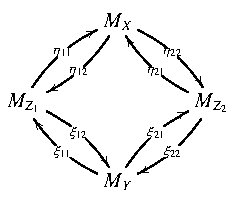
\includegraphics[width=0.56\textwidth]{figures/Fig_182_PDF291_Book279.pdf}
  \caption{粘合矩阵分解的极小模型箭图（原书 p.279）}\label{fig:glued-mf-minimal-quiver}
\end{figure}
所有 $\xi_{ij}$、$\eta_{ij}$ 都具有形如 $(\phi_1,\phi_2,0)$ 的形式，其中 $\phi_1\otimes_{R_1}R_{12}=\phi_2\otimes_{R_2}R_{12}$。例如
\[
  \xi_{11}=\left(\left(
  \begin{pmatrix}0&-1\\X_1&0\end{pmatrix},
  \begin{pmatrix}0&-1\\X_2Z_2&0\end{pmatrix}\right),0\right).
\]
进一步确定 $A_\infty$ 结构可得
\[
  \mu(\xi_{12},\eta_{12},\xi_{22},\eta_{22})=1_{M_X},
\]
并且 $\mathrm{MF}^{\pm}(M,M)$ 与四标记点球面上正方形四边的自同态环之间存在 $A_\infty$ 同构。对应关系图示如下：
\begin{figure}[H]\centering
  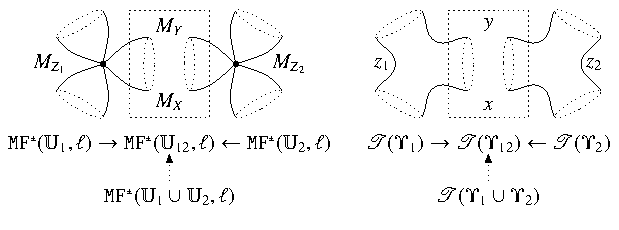
\includegraphics[width=0.93\textwidth]{figures/Fig_183_PDF292_Book280.pdf}
  \caption{Landau--Ginzburg 模型粘合与曲面范畴粘合的对应（原书 p.280）}\label{fig:glued-mf-surface-diagrams}
\end{figure}
两侧的图式都是由等价图式取同伦极限得到，因此
\[
  \mathrm{MF}^{\pm}(X,\ell)\cong_\infty
  \mathrm{topFuk}^{\pm}(S^2,\{0,1,\infty,p\}).
\]

这一思路可推广到亏格更高、标记点更多的曲面。取 $\mathbb Z^2$ 中一个凸格多边形，其内部有 $g$ 个格点、边界上有 $n$ 个格点，并把它放在 $\mathbb Z^3$ 中高度 $z=1$ 的平面上。令 $P$ 为多边形中的格点集，对每个 $p\in P$，记其坐标为 $(a_p,b_p,1)$。

选取一个三角剖分 $T$，把多边形分成基本三角形。基本三角形是 $v=\{r,s,t\}\subset P$，除顶点外不含其他格点；等价地，$r,s,t$ 构成 $\mathbb Z^3$ 的一组基。对每个三角形定义子环
\[
  R_v=\mathbb C[X^iY^jZ^k\mid a_pi+b_pj+k\ge0,\ p\in v],
  \qquad U_v=V(R_v).
\]
因为 $r,s,t$ 构成 $\mathbb Z^3$ 的一组基，$R_v$ 同构于三元多项式环，故 $U_v\cong\mathbb C^3$。$R_v$ 的生成元是单项式 $X^iY^jZ^k$，其中 $(i,j,k)$ 是 $r,s,t$ 的对偶基。把这些单项式记作 $U_v,V_v,W_v$。由于 $r,s,t$ 都位于平面 $z=1$，有
\[
  Z=U_vV_vW_v.
\]

对每条边 $e=\{r,s\}$，定义
\[
  R_e=\mathbb C[X^iY^jZ^k\mid a_pi+b_pj+k\ge0,\ p\in e].
\]
它同构于 $\mathbb C[U_v,V_v,W_v,W_v^{-1}]$，因为此处少了第三个不等式条件。因此 $U_e=V(R_e)\cong\mathbb C^2\times\mathbb C^*$。若 $e$ 是三角形 $v$ 的一条边，则 $R_v\subset R_e$，对偶地 $U_e\subset U_v$。沿公共边识别各个 $U_e$ 并粘合所有 $U_v$，得到一个三维光滑环簇 $Y_T$。所有这些环都是 $\mathbb C[X^{\pm1},Y^{\pm1},Z^{\pm1}]$ 的子环，并且都含有 $\ell=Z$。因此 $\ell$ 是 $Y_T$ 上的全局函数，我们得到 Landau--Ginzburg 模型 $(Y_T,\ell)$。

现在考察三角剖分的对偶图 $\Gamma_T$。每个三角形对应一个节点，每条剖分边对应一条对偶边；若原边位于多边形边界上，则对应的对偶边是半开边。每个节点 $v$ 带有 Landau--Ginzburg 模型 $(U_v,\ell)$，每条边带有模型 $(U_e,\ell)$。若边 $e$ 与节点 $v$ 相连，则有嵌入 $U_e\hookrightarrow U_v$。
\begin{figure}[H]\centering
  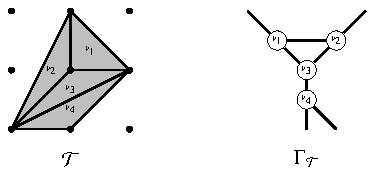
\includegraphics[width=0.79\textwidth]{figures/Fig_184_PDF293_Book281.pdf}
  \caption{三角剖分及其对偶图（原书 p.281）}\label{fig:triangulation-dual-graph}
\end{figure}
对每个节点 $v$ 和边 $e$，有两个矩阵分解范畴及一个限制函子：
\[
  \mathcal M(U_v):=\mathrm{MF}^{\pm}(U_v,\ell)
  \longrightarrow
  \mathcal M(U_e):=\mathrm{MF}^{\pm}(U_e,\ell).
\]
由此得到一个 $A_\infty$ 范畴图式；$(Y_T,\ell)$ 的矩阵分解范畴可以解释为该图式的同伦极限。

$A$ 侧则沿对偶图 $\Gamma_T$ 构造管状邻域 $\Sigma_T$，得到一个带穿孔曲面，其亏格等于图中的圈数，穿孔数等于管状图的腿数。用多边形来表述，亏格等于多边形内部格点数，腿数等于边界格点数。可用节点周围的开星形邻域 $\Upsilon_v$ 和边的开邻域 $\Upsilon_e$ 覆盖该图。应用函子 $T$ 后，也得到 Fukaya 范畴图式，其同伦极限为 $\mathrm{topFuk}^{\pm}(\Sigma_T)$。下图展示了两个对应的图式：
\begin{figure}[H]\centering
  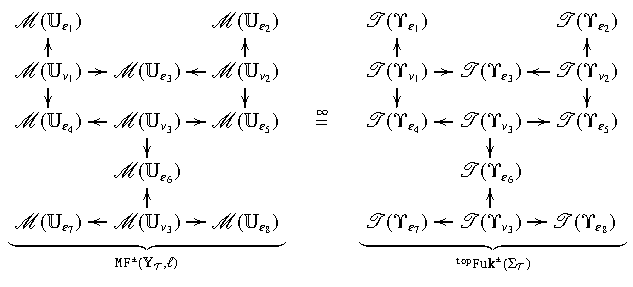
\includegraphics[width=0.98\textwidth]{figures/Fig_185_PDF293_Book281.pdf}
  \caption{矩阵分解范畴与拓扑 Fukaya 范畴图式的对应（原书 p.281）}\label{fig:triangulation-category-diagrams}
\end{figure}
核心想法是：这两个图式 $A_\infty$ 等价，因此它们的极限也等价。
\end{example}

\begin{theorem}{Sibilla--Pascaleff--Lee 定理}{polygon-gluing-mirror-equivalence}
设 $T$ 是一个凸格多边形的三角剖分，多边形内部有 $g$ 个格点、边界有 $n$ 个格点，则
\[
  \mathrm{MF}^{\pm}(Y_T,\ell)\cong_\infty\mathrm{topFuk}^{\pm}(\Sigma_T),
\]
其中 $\Sigma_T$ 是亏格为 $g$、有 $n$ 个标记点的闭带标记曲面。
\end{theorem}
\begin{proof}[证明思路]
为使上述构想成立，必须转到适当完备化后的范畴。先在完备化的设定中作粘合，再把所得等价限制到紧对象子范畴，就得到未完备化版本之间的等价。更多细节见 Pascaleff 和 Sibilla\bookcite{204}。Lee 的另一种方法是分别识别两侧的生成元，见\bookcite{155}。\hfill$\square$
\end{proof}

\section{覆盖}\label{sec:covers}
\takeaway{覆盖 $\pi$ 拉回弧系给出严格 $A_\infty$ 函子，而群作用与叉积 $A\star G$ 给出覆盖曲面的 gentle 代数；据此为商栈 $[\mathbb C^3/G]$ 构造带栈镜像，其标记点数由特征标 $\lambda_X,\lambda_Y,\lambda_Z$ 的稳定子决定。}
\begin{definition}{带标记曲面间的覆盖映射}{marked-surface-cover}
设 $(S_1,M_1)$、$(S_2,M_2)$ 是带标记曲面。映射 $\pi\colon S_1\to S_2$ 称为覆盖映射\index{daibiaojiqumianjiandefugaiyingshe@带标记曲面间的覆盖映射|hyperpage}，若它是一个分支覆盖，满足 $\pi(M_1)=M_2$，且所有分支点都位于 $M_2$。覆盖次数定义为 $p\in S_2\setminus M_2$ 的原像点数 $|\pi^{-1}(p)|$。
\end{definition}

若 $A_2$ 是剖分 $(S_2,M_2)$ 的弧系，则沿 $\pi$ 拉回 $A_2$，得到剖分 $(S_1,M_1)$ 的弧系 $A_1$。$A_1$ 中任意两条弧之间的角态射都会映到 $S_2$ 中的一个角态射。因此，$\pi$ 诱导 gentle 范畴之间的严格 $A_\infty$ 函子
\[
  F_\pi\colon\mathrm{Gtl}^{\pm}A_1\longrightarrow\mathrm{Gtl}^{\pm}A_2,
  \qquad a\longmapsto\pi(a),\quad\alpha\longmapsto\pi(\alpha),
\]
并可扩张为导出范畴或相应拓扑 Fukaya 范畴之间的函子。类似地，覆盖 $\pi$ 的自同构群
\[
  G=\{\phi\colon S_1\to S_1\mid \pi\phi=\pi\}
\]
作用在弧系 $A_1$ 上，由此也得到严格 $A_\infty$ 函子对 $\mathrm{Gtl}^{\pm}A_1$ 的作用。现在反过来考虑这个构造。

\begin{definition}{群作用的 $A_\infty$ 代数叉积}{ainfty-smash-product}
设 $A$ 是一个 $A_\infty$ 代数，有限群 $G$ 通过严格 $A_\infty$ 同构作用于 $A$。叉积\index{chaji@叉积|hyperpage}代数定义为 $A\star G:=A\otimes\mathbb CG$，其 $A_\infty$ 乘积为
\[
  \mu(a_1\otimes g_1,\ldots,a_k\otimes g_k)
  =\mu(a_1,g_1\cdot a_2,\ldots,g_1\cdots g_{k-1}\cdot a_k)
  \otimes g_1\cdots g_k.
\]
容易验证，这些乘积满足 $A_\infty$ 公理。
\end{definition}

设 $A=\mathbb C Q/I$ 是由带标记曲面 $(S,M)$ 上弧系 $A$ 所给出的 gentle $A_\infty$ 代数，并且阿贝尔群 $G$ 的作用固定各顶点、只对每个角乘以一个标量。具体说，对每个 $\alpha\in Q_1$，存在一个特征标 $\lambda_\alpha\in\widehat G=\mathrm{Grp}(G,\mathbb C^*)$，使得 $g\cdot\alpha=\lambda_\alpha(g)\alpha$；若 $\alpha_1,\ldots,\alpha_k$ 是某个多边形的各角，则 $\lambda_{\alpha_1}\cdots\lambda_{\alpha_k}=1$。

\begin{theorem}{覆盖与 gentle 代数叉积}{gentle-cover-smash-product}
在上述设定下，
\[
  A\star G\cong\mathrm{Gtl}^{\pm}\widetilde A,
\]
其中 $\widetilde A$ 是 $A$ 沿覆盖 $\pi\colon\widetilde S\to S$ 拉回所得的弧系。
\end{theorem}
\begin{proof}[证明思路]
对每个 $\lambda\in\widehat G$ 及 $a\in Q_0$，定义
\[
  e_\lambda:=\frac1{|G|}\sum_{g\in G}\lambda(g)g\in\mathbb CG,
  \qquad a_\lambda:=a\otimes e_\lambda\in A\star G.
\]
$e_\lambda$ 构成 $\mathbb CG$ 的一组正交幂等基，而 $a_\lambda$ 构成 $A\star G$ 的一组完备正交幂等元。把 $a_\lambda$ 作为新箭图 $\widetilde Q$ 的顶点。若 $\alpha\in Q_1$ 是一条从 $b=t(\alpha)$ 到 $a=h(\alpha)$ 的角，则
\[
\begin{aligned}
  \alpha\otimes1
  &=\left(\sum_{\kappa\in\widehat G}a\otimes e_\kappa\right)
    (\alpha\otimes1)
    \left(\sum_{\lambda\in\widehat G}b\otimes e_\lambda\right)\\
  &=\sum_{\kappa,\lambda\in\widehat G}
    (a\otimes e_\kappa)(\alpha\otimes e_{\kappa\lambda_\alpha})
    (b\otimes e_\lambda)\\
  &=\sum_{\kappa\in\widehat G}
    (a\otimes e_\kappa)(\alpha\otimes1)(b\otimes e_{\kappa\lambda_\alpha})\\
  &=\sum_{\kappa\in\widehat G}a_\kappa(\alpha\otimes1)b_{\kappa\lambda_\alpha}.
\end{aligned}
\]
因此 $\alpha\otimes1$ 分解为 $\widetilde Q$ 中 $|G|$ 条新箭 $\alpha_\kappa$，其头尾满足
\[
  h(\alpha_\kappa)=h(\alpha)_\kappa,
  \qquad t(\alpha_\kappa)=t(\alpha)_{\kappa\lambda_\alpha}.
\]
若 $\alpha_1,\ldots,\alpha_k$ 是 $S$ 中某个多边形的各角，则对每个 $\kappa\in\widehat G$，用下列各角作为边界可构造一个新的多边形：
\[
  (\alpha_1)_\kappa,\quad
  (\alpha_2)_{\kappa\lambda_{\alpha_1}},\quad\ldots,\quad
  (\alpha_k)_{\kappa\lambda_{\alpha_1}\cdots\lambda_{\alpha_{k-1}}}.
\]
把这些多边形粘合起来，得到新曲面 $\widetilde S$ 及其弧系 $\widetilde A=\widetilde Q_0$，相应 gentle $A_\infty$ 代数同构于 $A\star G$。\hfill$\square$
\end{proof}

\begin{example}[三标记球面的三重覆盖]\label{ex:threefold-pants-cover}
取一个有三个标记点的球面，并构造一个以环面为覆盖空间、以这三个标记点为分支点的三重覆盖。球面上的三角形给出弧系 $A_2=\{x,y,z\}$；沿覆盖拉回后得到弧系
\[
  A_1=\{x_1,x_2,x_3,\ldots,z_1,z_2,z_3\}.
\]
可以把它画成平面上的周期弧系，其基本区域由六个三角形组成。覆盖自同构群为 $\mathbb Z_3$，并循环置换各弧的下标。
\begin{figure}[H]\centering
  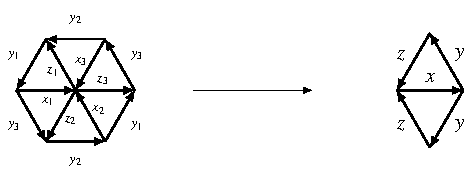
\includegraphics[width=0.89\textwidth]{figures/Fig_186_PDF296_Book284.pdf}
  \caption{裤子曲面的弧系在三重覆盖下的拉回（原书 p.284）}\label{fig:threefold-pants-cover}
\end{figure}

令 $G=\mathbb Z_3=\langle g\mid g^3=1\rangle$ 作用于
\[
  A=\mathrm{Gtl}^{\pm}A_2,
\]
使每个角都具有相同权重，即 $g\cdot\xi_i=e^{2\pi i/3}\xi_i$，$g\cdot\eta_i=e^{2\pi i/3}\eta_i$，$g\cdot\zeta_i=e^{2\pi i/3}\zeta_i$。于是 $A\star G$ 同构于上述覆盖曲面的 gentle 代数。
\begin{figure}[H]\centering
  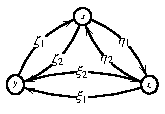
\includegraphics[width=0.68\textwidth]{figures/Fig_187_PDF296_Book284.pdf}
  \caption{三阶群作用下的 gentle 代数箭图（原书 p.284）}\label{fig:threefold-smash-quiver}
\end{figure}
\end{example}

覆盖方法可以为穿孔曲面构造带栈镜像。取有限阿贝尔群 $G$ 对 $\mathbb C^3$ 的对角作用。设对应的坐标特征标为 $\lambda_X,\lambda_Y,\lambda_Z\in\widehat G$，并满足
\[
  \lambda_X\lambda_Y\lambda_Z=1.
\]
此时函数 $XYZ$ 不变，所以它可以视为商栈 $[\mathbb C^3/G]$ 上的函数，并可考察相应矩阵分解。代数上，这些就是非交换 Landau--Ginzburg 模型 $(\mathbb C[X,Y,Z]\star G,XYZ)$ 的矩阵分解。

环 $B=\mathbb C[X,Y,Z]\star G$ 可以用一个箭图描述：顶点 $v_\phi$ 由 $\widehat G$ 编号，且有 $3|G|$ 条箭 $X_\phi,Y_\phi,Z_\phi$，分别连接 $v_\phi$ 与 $v_{\phi\lambda_X},v_{\phi\lambda_Y},v_{\phi\lambda_Z}$。这些箭之间的关系来自变量的交换关系：
\[
\begin{aligned}
  X_{\phi\lambda_Y}Y_\phi-Y_{\phi\lambda_X}X_\phi&=0,\\
  Y_{\phi\lambda_Z}Z_\phi-Z_{\phi\lambda_Y}Y_\phi&=0,\\
  Z_{\phi\lambda_X}X_\phi-X_{\phi\lambda_Z}Z_\phi&=0.
\end{aligned}
\]
正如每条箭在新箭图中有 $|G|$ 个对应物，标准矩阵分解 $M_X,M_Y,M_Z$ 也各有 $|G|$ 个版本。例如
\[
  M_{X_\phi}=\left(v_\phi B\oplus v_{\phi\lambda_X}B[1],
  \begin{pmatrix}
    0&Z_{\phi\lambda_Y\lambda_X}Y_{\phi\lambda_X}\\
    X_\phi&0
  \end{pmatrix}\right).
\]
基本态射 $\zeta_1\colon M_X\to M_Y$ 和 $\zeta_2\colon M_X\to M_Y$ 变为
\[
  \zeta_{1,\phi}\colon M_{X_\phi}\longrightarrow M_{Y_{\phi\lambda_Z}},
  \qquad
  \zeta_{2,\phi}\colon M_{Y_\phi}\longrightarrow M_{X_\phi}.
\]
% [Tutor Note: 原文把 $\zeta_1,\zeta_2$ 都写作 $M_X\to M_Y$，但紧接着的 $\zeta_{2,\phi}:M_{Y_\phi}\to M_{X_\phi}$ 方向相反；由上一节 $\mu(\zeta_1,\xi_1,\eta_1)=1_x$ 的循环结构，$\zeta_1,\zeta_2$ 中必有一个反向（原书 p.284 笔误），引用时以上标方向公式为准。]
这 $2|G|$ 个态射在箭图中组成 $|\widehat G/\langle\lambda_Z\rangle|$ 个环。

\begin{theorem}{阿贝尔商栈的镜像曲面}{abelian-stacky-pants-mirror}
若 $G\subset\mathrm{SL}_3(\mathbb C)$ 对 $\mathbb C^3$ 作对角作用，则
\[
  D^\pi\mathrm{MF}^{\pm}([\mathbb C^3/G],XYZ)
  \cong_\infty\mathrm{topFuk}^{\pm}(S,M),
\]
其中曲面 $S$ 的标记点数为
\[
  n=\frac{|G|}{|\langle\lambda_X\rangle|}
    +\frac{|G|}{|\langle\lambda_Y\rangle|}
    +\frac{|G|}{|\langle\lambda_Z\rangle|},
\]
其 Euler 示性数为 $n-|G|$。
\end{theorem}
\begin{proof}[证明思路]
与裤子曲面的情形相同，可以证明 $M_{X_\phi},M_{Y_\phi},M_{Z_\phi}$ 分裂生成 $D^\pi\mathrm{MF}^{\pm}([\mathbb C^3/G],XYZ)$。这些对象的自同态环是 $M_X\oplus M_Y\oplus M_Z$ 的自同态环与 $G$ 的叉积。由裤子曲面的镜像对称可知，这就是一个 gentle 代数与 $G$ 的叉积，也就是某个覆盖曲面的 gentle 代数。该曲面由 $2|G|$ 个三角形、$3|G|$ 条弧组成。其标记点数等于由 $\xi$、$\eta$ 或 $\zeta$ 组成的极小环路数；如上所见，这个数正是
\[
  n=\frac{|G|}{|\langle\lambda_X\rangle|}
    +\frac{|G|}{|\langle\lambda_Y\rangle|}
    +\frac{|G|}{|\langle\lambda_Z\rangle|}.
\]
\hfill$\square$
\end{proof}

\begin{example}[循环群作用的带栈镜像]\label{ex:cyclic-stacky-mirror}
令 $\mathbb Z_{2g+1}$ 以权重
\[
  \left(e^{2\pi i/(2g+1)},e^{2\pi i/(2g+1)},e^{-4\pi i/(2g+1)}\right)
\]
作用于 $\mathbb C[X,Y,Z]$。所得带栈 Landau--Ginzburg 模型的镜像是一个有三个标记点的曲面 $(S,M)$，其 Euler 示性数为 $3-(2g+1)=2-2g$，所以曲面亏格为 $g$。该曲面可以画成粘合在一起的 $2(2g+1)$ 边形：
\begin{figure}[H]\centering
  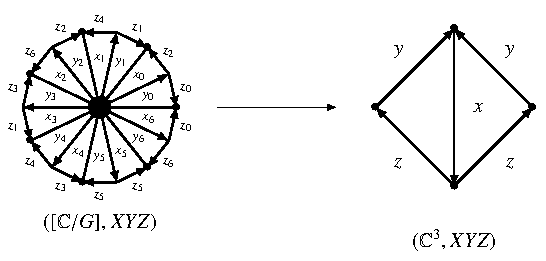
\includegraphics[width=0.9\textwidth]{figures/Fig_188_PDF297_Book285.pdf}
  \caption{循环群商栈及其裤子曲面镜像（原书 p.285）}\label{fig:cyclic-stacky-pants-mirror}
\end{figure}
\end{example}

\section{二聚体模型}\label{sec:dimer-models}
\takeaway{二聚体模型是弧系带循环定向的版本，镜面对偶在组合层面交换标记点与锯齿圈；Jacobi 代数 $(\mathrm{Jac}\,Q,\ell)$ 的矩阵分解的自同态环 $A_\infty$ 同构于 $\mathrm{Gtl}^{\pm}Q^\vee$，锯齿一致性保证这一镜像等价成立。}
我们可以把上述构造推广到其他非交换镜像。为此，先引入一些工具。

\begin{definition}{二聚体模型}{dimer-model}
二聚体模型\index{erjutimoxing@二聚体模型|hyperpage} $Q=(S,M,A)$ 由一个带标记曲面和一组剖分该曲面的弧组成，并要求每个多边形周围的弧都沿环形方向定向。把 $Q$ 看成嵌入曲面 $S$ 的箭图，其中 $Q_0=M$、$Q_1=A$。每个多边形给出 $Q$ 中的一个环路，把这些环路组成集合 $Q_2$。它是两个子集的并：$Q_2^+$ 由逆时针定向的环路组成，$Q_2^-$ 由顺时针定向的环路组成。
\end{definition}

\begin{note}\label{note:dimer-bipartite-origin}
二聚体模型的概念最初来自统计物理，原本指嵌入曲面的二分图\bookcite{137,132}。该图是弧系的对偶带状图：在每个顺时针多边形内放一个白点，在每个逆时针多边形内放一个黑点；相邻面的节点以边相连。
\end{note}

\begin{definition}{镜面（二聚体）对偶}{dimer-duality}
在二聚体模型集合上有一种对偶，称为镜面对偶\index{jingmianduiou@镜面对偶|hyperpage}\bookcite{121}或二聚体对偶\index{erjutiduiou@二聚体对偶|hyperpage}\bookcite{36,35}。其步骤如下：
\begin{enumerate}[label=(\roman*)]
  \item 沿弧把二聚体 $Q$ 切开；
  \item 翻转顺时针多边形中弧的定向；
  \item 按照相容的定向把所有部分重新粘合。
\end{enumerate}
所得新二聚体记为 $Q^\vee$。这一过程是对合，即 $Q^{\vee\vee}=Q$；$Q^\vee$ 也称为 $Q$ 的镜像二聚体\index{jingxiangerjuti@镜像二聚体|hyperpage}。
\end{definition}

\begin{example}[环面二聚体的对偶]\label{ex:torus-dimer-mirror}
从一个把环面剖分成两个三角形的二聚体出发，施行二聚体对偶后得到一个位于三标记球面上的二聚体：
\begin{figure}[H]\centering
  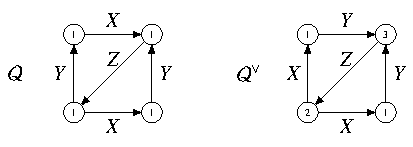
\includegraphics[width=0.66\textwidth]{figures/Fig_189_PDF298_Book286.pdf}
  \caption{环面二聚体及其镜像二聚体（原书 p.286）}\label{fig:torus-dimer-mirror}
\end{figure}
\end{example}

\begin{example}[更多二聚体对偶的例子]\label{ex:dimer-duality-examples}
下图给出文献\bookcite{36}中的另外四个例子。上排是四个二聚体：前两个嵌入环面，第三个嵌入亏格为 $2$ 的曲面，第四个位于球面。它们的镜像都嵌入环面，见下排。注意，前两个二聚体与其镜像同构，但这种同构并非显然。
\begin{figure}[H]\centering
  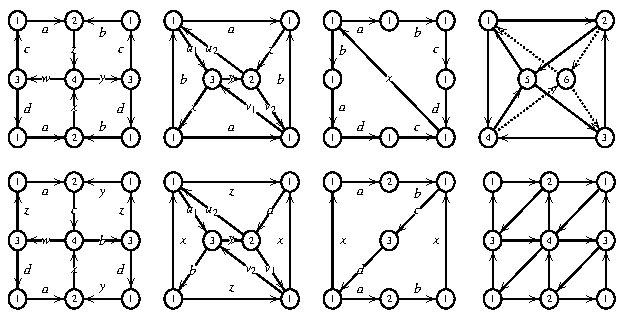
\includegraphics[width=0.99\textwidth]{figures/Fig_190_PDF299_Book287.pdf}
  \caption{四组二聚体及其镜像（原书 p.287）}\label{fig:four-dimer-duals}
\end{figure}
\end{example}

要记录二聚体对偶对亏格和标记点数的影响，需要引入锯齿路径\index{juchilujing@锯齿路径|hyperpage}的概念。

\begin{definition}{锯齿路径}{zigzag-path}
若路径 $a_1\cdots a_k$ 满足：当 $i$ 为偶数时，$a_i,a_{i+1}$ 在正向环路中相继出现；当 $i$ 为奇数时，它们在负向环路中相继出现，则称它为锯齿路径。换言之，这条路径在曲面上交替向左、向右转。从一条箭 $a$ 出发可以构造两条锯齿路径：锯齿射线先向左、再向右转；反锯齿射线先向右、再向左转。
\end{definition}

在对偶操作下，锯齿环路中的各条箭都会与镜像二聚体中的同一个标记点相接，因此二聚体对偶会交换标记点与锯齿环路：
\begin{figure}[H]\centering
  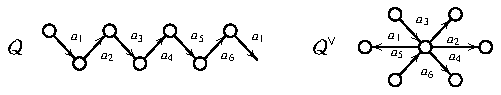
\includegraphics[width=0.64\textwidth]{figures/Fig_191_PDF299_Book287.pdf}
  \caption{锯齿路径及其在对偶二聚体中的表现（原书 p.287）}\label{fig:zigzag-path-duality}
\end{figure}

\begin{lemma}{二聚体对偶下的拓扑量}{dimer-duality-euler-characteristic}
设二聚体 $Q$ 有 $n$ 个标记点、$z$ 个锯齿环路，Euler 示性数为 $\chi$。则 $Q^\vee$ 有 $z$ 个标记点、$n$ 个锯齿环路，Euler 示性数为 $\chi-n+z$。
\end{lemma}

\begin{definition}{Jacobi 代数}{jacobi-algebra}
对二聚体 $Q$，可以构造一个非交换代数，称为它的 Jacobi 代数\index{jacobidaishu@Jacobi 代数|hyperpage}。它是箭图 $Q$ 的路径代数除以如下关系：对每条箭 $a$，令 $a\ell_a$ 和 $ar_a$ 是 $Q_2$ 中包含 $a$ 的两个环路，则令两条回路路径相等：
\[
  \mathrm{Jac}\,Q:=
  \frac{\mathbb C Q}{\langle \ell_a-r_a\mid a\in Q_1,\;a\ell_a\in Q_2^+,\;ar_a\in Q_2^-\rangle}.
\]
\begin{figure}[H]\centering
  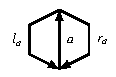
\includegraphics[width=0.42\textwidth]{figures/Fig_192_PDF299_Book287.pdf}
  \caption{一条箭及其所在的正、负向环路（原书 p.287）}\label{fig:dimer-jacobi-relation}
\end{figure}
这些关系表示：对每条箭，沿左侧环路返回与沿右侧环路返回，在代数中是相同的路径。
\end{definition}

\begin{lemma}{Jacobi 代数的中心元}{jacobi-central-element}
Jacobi 代数 $\mathrm{Jac}\,Q$ 含有一个中心元 $\ell$，并且对每个 $v\in Q_0$，$v\ell$ 都是 $Q_2$ 中的一个环路。
\end{lemma}
\begin{proof}[证明思路]
对每个 $v$，取一个从 $v$ 出发且代表 $Q_2$ 中环路的闭路 $\ell_v$。由于 Jacobi 关系，$\ell_v$ 在 $\mathrm{Jac}\,Q$ 中不依赖于闭路的具体选择。进一步，对任意路径 $p$，利用这些关系可得
\[
  \ell_{h(p)}p=p\ell_{t(p)}.
\]
因此 $\ell:=\sum_{v\in Q_0}\ell_v$ 是中心元。\hfill$\square$
\end{proof}

\begin{definition}{二聚体的 Landau--Ginzburg 模型}{dimer-landau-ginzburg}
二聚体 $Q$ 的 Landau--Ginzburg 模型\index{qdelandauginzburgmoxing@Q 的 Landau–Ginzburg 模型|hyperpage}是二元组 $(\mathrm{Jac}\,Q,\ell)$。
\end{definition}

\begin{example}[裤子曲面的 Jacobi 代数]
从例\ref{ex:torus-dimer-mirror} 中把环面剖分成两个三角形的二聚体 $Q$ 出发。其 Jacobi 代数是三元多项式环
\[
  \mathrm{Jac}\,Q=
  \frac{\mathbb C\langle X,Y,Z\rangle}
       {\langle XY-YX,\;XZ-ZX,\;YZ-ZY\rangle},
\]
中心元为 $\ell=XYZ$。它的 Landau--Ginzburg 模型是裤子曲面的镜像，因此 $Q^\vee$ 位于一个有三个标记点的球面上。
\end{example}
% [Tutor Note: 直觉上，二聚体对偶就是镜像对称的组合版本：A 侧的弧系与 B 侧 Jacobi 代数的矩阵分解互为镜像，锯齿圈（箭的极大交替路径）在对偶下变成标记点，这正是亏格与标记点数在对偶下互换的来源。]

这一构造也与覆盖相容。先考虑有一个穿孔的环面，并通过选取两个向量 $v_1,v_2\in\mathbb Z^2$ 来扩大其基本区域，令
\[
  S=\mathbb R^2/(\mathbb Z v_1+\mathbb Z v_2).
\]
取格点集 $M=\mathbb Z^2/(\mathbb Z v_1+\mathbb Z v_2)$ 作为标记点，\linebreak[3] 并取从每个标记点出发、方向向量分别为\linebreak $(1,0),(0,1),(-1,-1)$ 的箭组成弧系。对每个 $m\in M$，按方向把这些箭记为 $x_m,y_m,z_m$。总共有 $k=|\det(v_1,v_2)|$ 个标记点和 $3k$ 条箭，它们把环面剖分成 $2k$ 个三角形。把这个二聚体记为 $Q_{v_1,v_2}$。

注意，$M=\mathbb Z^2/(\mathbb Z v_1+\mathbb Z v_2)$ 本身也是一个群。令 $G=\mathrm{Hom}(M,\mathbb C^*)$，则 $M$ 是 $G$ 的特征群。可以定义 $G$ 在 $\mathbb C[X,Y,Z]$ 上的作用：
\[
  g\cdot X=g(1,0)X,\qquad
  g\cdot Y=g(0,1)Y,\qquad
  g\cdot Z=g(-1,-1)Z.
\]
这里 $(1,0),(0,1),(-1,-1)$ 都视为 $M$ 的元素，因此可以将 $g\in G=\mathrm{Hom}(M,\mathbb C^*)$ 作用于它们。

\begin{lemma}{覆盖环面二聚体的 Jacobi 代数}{cover-dimer-jacobi-algebra}
二聚体 $Q_{v_1,v_2}$ 的 Jacobi 代数同构于
\[
  \mathrm{Jac}\,Q_{v_1,v_2}\cong\mathbb C[X,Y,Z]\star G.
\]
\end{lemma}
\begin{proof}
代数 $\mathbb C[X,Y,Z]\star G$ 的箭图顶点是 $G$ 的特征，因而与 $M$ 中元素对应。其箭形如 $X_\phi,Y_\phi,Z_\phi$，其中 $\phi\in\widehat G$，自然对应于 $x_m,y_m,z_m$。因此存在自然满射
\[
  \mathbb C Q\longrightarrow\mathbb C[X,Y,Z]\star G.
\]
该映射通过 Jacobi 代数，因为 $\mathrm{Jac}\,Q$ 中的关系都形如 $x_\phi y_\psi-y_\phi x_\psi$（或把 $\{x,y,z\}$ 中其他两种变量配对得到的关系）；在映射下，这些关系变成 $[X,Y]e_\psi=0$。

Jacobi 代数中的关系说明，每条路径都由其起点与其中 $x,y,z$ 的数目唯一确定。因此，没有两条不同路径会映到 $\mathbb C[X,Y,Z]\star G$ 中的同一个元素，故上述映射也是单射。\hfill$\square$
\end{proof}

若把这些带栈 Landau--Ginzburg 模型视为非交换 Landau--Ginzburg 模型，就可以把镜像对称解释为二聚体对偶的一种实例。箭图 $Q=Q_{v_1,v_2}$ 中每条箭 $a$ 都自然对应于 $\ell\in\mathrm{Jac}\,Q$ 的一个矩阵分解：
\begin{figure}[H]\centering
  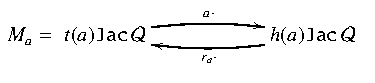
\includegraphics[width=0.38\textwidth]{figures/Fig_193_PDF301_Book289.pdf}
  \caption{由箭构造的 Jacobi 代数矩阵分解（原书 p.289）}\label{fig:arrow-matrix-factorization}
\end{figure}
由定理\ref{thm:abelian-stacky-pants-mirror}可知，矩阵分解 $M_a$ 的直和的自同态环 $A_\infty$ 同构于某个曲面弧系的 gentle 代数。直接计算可见，该弧系恰是镜像二聚体 $Q^\vee$ 所对应的弧系：
\[
  \mathrm{End}_{\mathrm{MF}^{\pm}(\mathrm{Jac}\,Q,\ell)}
  \left(\bigoplus_{a\in Q_1}M_a\right)
  \cong_\infty\mathrm{Gtl}^{\pm}Q^\vee.
\]

\begin{example}[环面覆盖与二聚体对偶]\label{ex:cyclic-dimer-duality}
令 $v_1=(g+1,g)$、$v_2=(g,g+1)$。此时
\[
  M=\mathbb Z^2/(\mathbb Z v_1+\mathbb Z v_2)
  \cong\mathbb Z/(2g+1)\mathbb Z=\langle(1,1)\rangle.
\]
取对偶生成元 $u\in\mathrm{Hom}(M,\mathbb C^*)$，令它把 $(1,1)$ 映到 $e^{2\pi i/(2g+1)}$。于是
\[
  u\cdot X=e^{2\pi i/(2g+1)}X,\qquad
  u\cdot Y=e^{2\pi i/(2g+1)}Y,\qquad
  u\cdot Z=e^{-4\pi i/(2g+1)}Z.
\]
\begin{figure}[H]\centering
  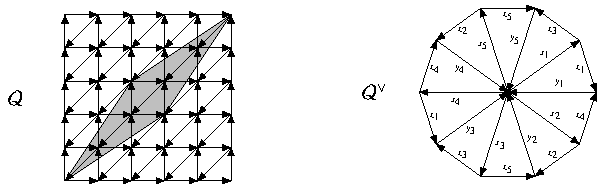
\includegraphics[width=0.86\textwidth]{figures/Fig_194_PDF301_Book289.pdf}
  \caption{互为镜像的两个环面二聚体（原书 p.289）}\label{fig:cyclic-dimer-dual}
\end{figure}
从二聚体角度看，$Q$ 的亏格为 $1$、有 $2g+1$ 个标记点；其对偶二聚体 $Q^\vee$ 的亏格为 $g$、有 $3$ 个标记点。这与例\ref{ex:cyclic-stacky-mirror}相同。
\end{example}

从这个例子可能会猜想，任意二聚体都具有这样的二聚体对偶性质；遗憾的是，并非如此。关键问题在于某些情形下 Jacobi 代数的性质不够好（例如整体维数不是有限的），因此必须给二聚体附加一些一致性条件\index{yizhixingtiaojian@一致性条件|hyperpage}。文献中研究过多种一致性条件\bookcite{180,63,42,126,33}；下面聚焦其中一个。

\begin{definition}{锯齿一致二聚体}{zigzag-consistent-dimer}
若对 $Q_1$ 中每条箭 $a$，锯齿射线与反锯齿射线在万有覆盖中除 $a$ 本身外不相交，则称二聚体 $Q$ 是锯齿一致\index{juchiyizhixing@锯齿一致性|hyperpage}的。
\end{definition}

\begin{example}[二聚体的一致性]
下表列出例\ref{ex:dimer-duality-examples}中八个二聚体的一致性性质：
\[
\begin{array}{c|cccc}
 &Q_1&Q_2&Q_3&Q_4\\\hline
\text{锯齿一致}&\text{是}&\text{否}&\text{是}&\text{否}\\
\text{镜像一致}&\text{是}&\text{否}&\text{否}&\text{是}
\end{array}
\]
对上排第二个二聚体，可以直接检查从 $z$ 出发的锯齿射线和反锯齿射线也会在 $x$ 处相交。
\end{example}

\begin{theorem}{锯齿一致二聚体的镜像等价}{zigzag-consistent-dimer-mirror}
若二聚体 $Q$ 锯齿一致，则
\[
  \mathrm{End}_{\mathrm{MF}^{\pm}(\mathrm{Jac}\,Q,\ell)}
  \left(\bigoplus_{a\in Q_1}M_a\right)
  \cong_\infty\mathrm{Gtl}^{\pm}Q^\vee.
\]
\end{theorem}
\begin{proof}[证明思路]
设 $M_a,M_b$ 是分别来自箭 $a,b$ 的两个矩阵分解，且 $ax_1\cdots x_kb$ 是一条锯齿路径。可以利用这条锯齿路径的反向路径构造一个从 $M_a$ 到 $M_b$ 的态射。这两条路径 $z^+,z^-$ 分别沿着锯齿路径两侧的正向环和负向环返回：
\begin{figure}[H]\centering
  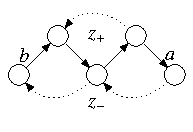
\includegraphics[width=0.48\textwidth]{figures/Fig_195_PDF302_Book290.pdf}
  \caption{锯齿路径两侧的正、负向回路（原书 p.290）}\label{fig:zigzag-positive-negative-paths}
\end{figure}
该态射的形状如下：
\begin{figure}[H]\centering
  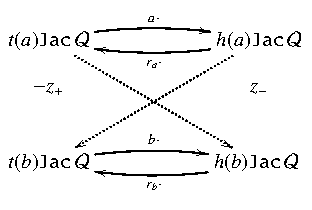
\includegraphics[width=0.58\textwidth]{figures/Fig_196_PDF302_Book290.pdf}
  \caption{由锯齿路径给出的矩阵分解态射（原书 p.290）}\label{fig:zigzag-mf-morphism}
\end{figure}
在二聚体对偶构造下，锯齿环路变成 $Q^\vee$ 中的标记点，而锯齿路径可视为绕这些标记点转向的角，换言之，就是 gentle 代数 $\mathrm{Gtl}^{\pm}Q^\vee$ 中的路径。若 $Q$ 锯齿一致，可以证明这一解释延拓为\linebreak $\mathrm{End}_{\mathrm{MF}^{\pm}(\mathrm{Jac}\,Q,\ell)}(\bigoplus_{a\in Q_1}M_a)$ 与 $\mathrm{Gtl}^{\pm}Q^\vee$ 之间的 $A_\infty$ 同构。证明的更多细节见\bookcite{36}。\hfill$\square$
\end{proof}

\begin{example}[两个正方形铺砌的环面]\label{ex:two-square-dimer}
取一个有两个标记点的环面，并用两个正方形铺砌。其对偶二聚体是有四个标记点的球面。容易验证，第一个二聚体是一致的：在万有覆盖中，锯齿射线是沿不同方向延伸的阶梯线，所以只能在一条箭上相交。第二个二聚体不一致，因为它位于球面上，锯齿射线总会多次相交。
\begin{figure}[H]\centering
  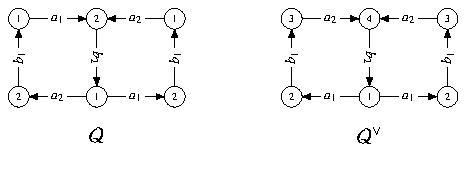
\includegraphics[width=0.86\textwidth]{figures/Fig_197_PDF303_Book291.pdf}
  \caption{环面上的二聚体及球面上的镜像二聚体（原书 p.291）}\label{fig:two-square-dimer-dual}
\end{figure}
其 Jacobi 代数为
\[
  \mathrm{Jac}\,Q:=
  \frac{\mathbb C\langle a_1,a_2,b_1,b_2\rangle}{I},
\]
其中 $I$ 由下列四个关系生成：
\[
\begin{aligned}
  a_1b_1a_2-a_2b_1a_1,&\qquad a_1b_2a_2-a_2b_2a_1,\\
  b_1a_1b_2-b_2a_1b_1,&\qquad b_1a_2b_2-b_2a_2b_1.
\end{aligned}
\]
中心元为 $\ell=a_1b_1a_2b_2+b_1a_2b_2a_1$。非交换 Landau--Ginzburg 模型 $(\mathrm{Jac}\,Q,\ell)$ 是四标记球面的镜像。
\begin{figure}[H]\centering
  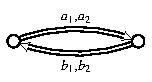
\includegraphics[width=0.43\textwidth]{figures/Fig_198_PDF303_Book291.pdf}
  \caption{构成 Jacobi 关系的两组平行箭（原书 p.291）}\label{fig:two-square-jacobi-arrows}
\end{figure}

正如裤子曲面的镜像是嵌入光滑三维空间 $\mathbb A^3$ 中的 Landau--Ginzburg 模型，这些 Jacobi 代数也应被视为非交换空间。若二聚体 $Q$ 一致且其曲面是环面，则 $\mathrm{Jac}\,Q$ 实际上与一个真正的交换空间——三维环簇 Calabi--Yau 簇——导出等价。该簇的 Newton 多边形各边的法向量，与二聚体万有覆盖中锯齿射线的方向一一对应（在万有覆盖中作图时，基本区域取为单位正方形）。关于三维环簇 Calabi--Yau 簇和二聚体模型的更多关系，见\bookcite{125,127,179}。
\end{example}

\begin{example}[三标记环面二聚体的镜像]\label{ex:five-zigzag-dimer}
取文献\bookcite{35}中的二聚体 $Q$。它嵌入有三个标记点的环面，而其镜像二聚体 $Q^\vee$ 位于有五个标记点的球面。
\begin{figure}[H]\centering
  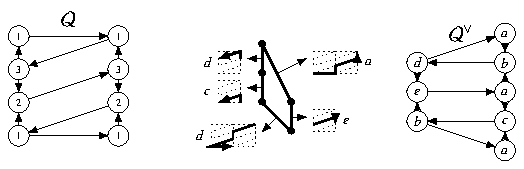
\includegraphics[width=0.94\textwidth]{figures/Fig_199_PDF304_Book292.pdf}
  \caption{环面二聚体、其镜像及 Newton 多边形（原书 p.292）}\label{fig:five-zigzag-dimer}
\end{figure}
二聚体 $Q$ 有五条锯齿路径，图中央画出了 Newton 多边形 $\square$，其边垂直于这些锯齿路径。Jacobi 代数 $\mathrm{Jac}\,Q$ 与第\ref{subsec:one-two-three-models}节中的三维环簇 $X^3_{\boxtimes}$ 导出等价。
\end{example}

\section{众多镜像}\label{sec:mirrors-galore}
\takeaway{同一带标记曲面可有三类镜像：Newton 多边形三角剖分给出的三维环簇、$[\mathbb C^3/G]$ 型的带栈 Landau--Ginzburg 模型，与锯齿一致二聚体给出的非交换 Landau--Ginzburg 模型；亏格与标记点数由多边形或二聚体的组合量算出。}
设 $(S,M)$ 是亏格为 $g$、有 $n$ 个内部标记点的带标记曲面。可以为它构造若干不同类型的镜像；每一类镜像也会因额外的组合数据而有不同选择。

\begin{itemize}
  \item \textbf{交换 Landau--Ginzburg 模型。}对 Newton 多边形作三角剖分，可以构造一个三维环簇 $X_{\boxtimes}^{3}$ 及其上的全局函数 $\ell$，并得到
  \[
    \mathrm{topFuk}^{\pm}(S,M)\simeq D^{\pi}\mathrm{MF}^{\pm}(X_{\boxtimes}^{3},\ell).
  \]
  曲面的标记点数等于多边形边界格点数，亏格等于多边形内部格点数。

  \item \textbf{带栈 Landau--Ginzburg 模型。}取有限阿贝尔群 $G\subset\mathrm{SL}_3(\mathbb C)$，可构造三维商栈 $[\mathbb C^3/G]$ 及其不变函数 $\ell=XYZ$，并有
  \[
    \mathrm{topFuk}^{\pm}(S,M)\simeq D^{\pi}\mathrm{MF}^{\pm}([\mathbb C^3/G],\ell).
  \]
  标记点数等于 $X,Y,Z$ 三个函数的稳定子群阶数之和，即
  \[
    n=|G_X|+|G_Y|+|G_Z|,
  \]
  而曲面的亏格为
  \[
    g=\frac12\bigl(|G|-|G_X|-|G_Y|-|G_Z|\bigr)+1.
  \]

  \item \textbf{非交换 Landau--Ginzburg 模型。}取一个锯齿一致的二聚体模型 $Q$，它给出 Jacobi 代数 $\mathrm{Jac}\,Q$ 及其中心元 $\ell$。每条箭 $a\in Q_1$ 对应于 $(\mathrm{Jac}\,Q,\ell)$ 的一个矩阵分解 $M_a$，也对应于镜像二聚体 $Q^{\vee}$ 中的一条弧 $a$，从而给出 $\mathrm{topFuk}^{\pm}(S,M)$ 中的对象 $L_a$。两侧的生成子范畴之间有 $A_{\infty}$ 同构：
  \[
    D^{\pi}\mathrm{MF}^{\pm}(\mathrm{Jac}\,Q,\ell)\supset
    \langle M_a\mid a\in Q_1\rangle
    \cong_\infty
    \langle L_a\mid a\in Q^{\vee}_1\rangle
    \subset\mathrm{topFuk}^{\pm}(S,M).
  \]
  曲面的标记点数 $n$ 等于 $Q$ 的锯齿环路数，曲面亏格为
  \[
    g=\frac12\bigl(\#Q_1-\#Q_2-n\bigr)+1.
  \]
\end{itemize}

\section{习题}\label{sec:gluing-exercises}

\begin{exercise}\label{exer:gluing-min-arcs}
设 $(S,M)$ 是亏格为 $g$ 的带标记曲面，有 $m$ 个边界分支，第 $i$ 个边界分支上有 $b_i$ 个标记点（$1\le i\le m$），并有 $k$ 个内部标记点。写出将曲面剖分所需弧数的最小值公式。
\end{exercise}

\begin{exercise}\label{exer:gluing-linear-quiver-surface}
找一个曲面及其弧系，使相应 gentle 代数是下图箭图的路径代数：
\begin{figure}[H]\centering
  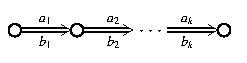
\includegraphics[width=0.43\textwidth]{figures/Fig_200_PDF305_Book293.pdf}
  \caption{练习 9.2 中的箭图（原书 p.293）}
\end{figure}
其关系为 $a_{i+1}a_i=b_{i+1}b_i=0$，且所有箭的次数均为 $0$。用 $k$ 表示该曲面的亏格和边界分支数。
\end{exercise}

\begin{exercise}\label{exer:gluing-self-intersecting-string}
设曲线 $\gamma$ 从两个不同的标记点出发，并自交一次，围成一个不可缩的环。确定相应弦对象在 $D\mathrm{Gtl}^{\pm}A$ 中的自同态环。
\end{exercise}

\begin{exercise}\label{exer:gluing-polygon-hocolim}
取一个多边形并将其三角剖分。利用这一三角剖分，把多边形的 Fukaya 范畴写成若干个下图所示范畴的同伦余极限：
\begin{figure}[H]\centering
  \includegraphics[width=0.28\textwidth]{figures/Fig_201_PDF305_Book293.pdf}
  \caption{练习 9.4 中的基本箭图范畴（原书 p.293）}
\end{figure}
\end{exercise}

\begin{exercise}\label{exer:gluing-cylinder-two-marks}
将例\ref{ex:cylinder-tubular-gluing}推广到圆柱两侧各有两个标记点的情形，并完成相应构造。
\end{exercise}

\begin{exercise}\label{exer:gluing-local-p2}
考虑由 $(1,0,1)$、$(0,1,1)$ 和 $(-1,-1,1)$ 张成的多边形，并通过从顶点连接到 $v_0=(0,0,1)$ 来三角剖分。相应的光滑三维簇 $X_{\boxtimes}^{3}$ 是 $\mathbb P^2$ 的反典范线丛全空间；令 $D=\mathbb P^2$ 为对应于 $v_0$ 的除子。
\begin{enumerate}[label=(\roman*)]
  \item 确定与 $(X_{\boxtimes}^{3},\ell)$ 镜像的曲面 $S_{g,n}$ 的亏格和穿孔数。
  \item 在下列识别下，求出与结构层 $\mathcal O_D$ 的像相对应的 $\ell$ 的矩阵分解 $M$：
  \[
    \mathrm{MF}^{\pm}(X_{\boxtimes}^{3},\ell)
    =D_{\mathrm{Sing}}\bigl(\ell^{-1}(0)\bigr)
    =\frac{D\mathrm{Coh}\bigl(\ell^{-1}(0)\bigr)}
    {\mathrm{Perf}\bigl(\ell^{-1}(0)\bigr)}.
  \]
  提示：把 $\mathrm{MF}^{\pm}(\mathbb C^3,XYZ)$ 中形如 $M_X$ 的矩阵分解粘合起来。
  \item 利用同伦极限的解释，确定曲面 $S_{g,n}$ 上与 $M$ 对应的曲线。
\end{enumerate}
\end{exercise}

\begin{exercise}\label{exer:gluing-smash-product}
验证有限群对 $A_{\infty}$ 代数的作用所定义的叉积 $A\mathbin{\star}G$，按定义\ref{def:ainfty-smash-product} 的构造仍是一个 $A_{\infty}$ 代数。
\end{exercise}

\begin{exercise}\label{exer:gluing-klein-stacky-mirror}
令 $G=\mathbb Z_2\times\mathbb Z_2$ 作用于 $\mathbb C^3$，作用为
\[
  (a,b)\cdot(X,Y,Z)=\bigl((-1)^aX,(-1)^bY,(-1)^{a+b}Z\bigr).
\]
求带栈 Landau--Ginzburg 模型 $([\mathbb C^3/G],XYZ)$ 的镜像，并将其描述为三穿孔球面上的覆盖。同时，给出满足 $\mathrm{Jac}\,Q\cong\mathbb C[X,Y,Z]\mathbin{\star}G$ 的二聚体模型 $Q$。
\end{exercise}

\begin{exercise}\label{exer:gluing-dimer-mutation}
设 $Q$ 是锯齿一致的二聚体模型，$v\in Q_0$ 是一个顶点，有两条箭 $a_1,a_2$ 指向 $v$，另有两条箭 $b_1,b_2$ 从 $v$ 指出。通过反转这些箭并为路径 $b_i a_j$ 加入新箭来变异顶点，最后删去所有二环。局部变异如下图所示：
\begin{figure}[H]\centering
  \includegraphics[width=0.46\textwidth]{figures/Fig_202_PDF306_Book294.pdf}
  \caption{二聚体模型的顶点变异（原书 p.294）}
\end{figure}
证明变异后的二聚体模型 $\mu_v Q$ 仍然锯齿一致。
\end{exercise}

\begin{exercise}\label{exer:gluing-z3-dimer}
令 $G=\mathbb Z_3=\langle g\mid g^3=1\rangle$ 作用于 $\mathbb C^3$，且
\[
  g\cdot(X,Y,Z)=\bigl(e^{2\pi i/3}X,e^{2\pi i/3}Y,e^{2\pi i/3}Z\bigr).
\]
代数 $\mathbb C[X,Y,Z]\mathbin{\star}G$ 可表示为带关系的下图箭图：
\begin{figure}[H]\centering
  \includegraphics[width=0.4\textwidth]{figures/Fig_203_PDF306_Book294.pdf}
  \caption{练习 9.10 中的箭图（原书 p.294）}
\end{figure}
\begin{enumerate}[label=(\roman*)]
  \item 把 $Q$ 画成环面上的二聚体模型，使得 $\mathrm{Jac}\,Q\cong\mathbb C[X,Y,Z]\mathbin{\star}G$。
  \item 证明维数向量 $\alpha=(1,1,1)$、稳定参数 $\theta=(-2,1,1)$ 对应的模空间 $M_\theta(\mathrm{Jac}\,Q,\alpha)$ 同构于习题\ref{exer:gluing-local-p2} 中的簇。
  \item 求一个矩阵分解 $M$，使其对应于中心 $\mathbb P^2$ 的结构层。
\end{enumerate}
\end{exercise}

\chapterreview{%
\textbf{全章地位。}本章是全书构造的中枢。它用带标记曲面与生成弧系把曲面的 partially wrapped Fukaya 范畴完全组合化，得到只依赖多边形剖分的 $\mathrm{topFuk}^{\pm}(S,M)$，同时把 Kontsevich 关于“wrapped Fukaya 范畴是拉格朗日骨架上的范畴层”的设想在一维情形下兑现。此前的 gentle 代数、矩阵分解与二聚体在此合流，此后的分次版本、稳定性与变形都以本章的模型为出发点。

\textbf{知识脉络。}带标记曲面 $\to$ 生成弧系 $\to$ 箭图 $Q_A$ 与 gentle $A_\infty$ 代数 $\mathrm{Gtl}^{\pm}A$（面状路径置零，闭多边形贡献高阶乘积）$\to$ 换弧不变性（扭曲完备化与 Hatcher 翻转）$\to$ 定义 $\mathrm{topFuk}^{\pm}:=D\mathrm{Gtl}^{\pm}A$ $\to$ 用弧与角缝合曲线，得弦对象与带对象（交点为态射，多边形计数乘积）$\to$ 沿带状图（协变余层、同伦余极限）与管状图（反变层、同伦极限）粘合 $\to$ 以裤子曲面为基本构件做镜像并粘出高亏格曲面 $\to$ 覆盖与叉积 $A\star G$ $\to$ 二聚体与 Jacobi 代数。主线是“局部可算、整体靠粘合”。

\textbf{核心结论。}（1）$\mathrm{topFuk}^{\pm}(S,M)=D\mathrm{Gtl}^{\pm}A$ 与弧系无关；换弧归结为把反向弧识别为 $a[1]$，再由 Hatcher 定理化为四边形的对角翻转。（2）开曲线的同伦类实现为弦对象，闭曲线连同绕行变换实现为带对象 $B(L,T^\lambda)$；带对象间的态射由交点给出，乘积由曲线围成的浸入多边形计数，这正是 Fukaya 范畴的组合影子。（3）沿带状图的 $R$ 是余层，同伦余极限还原整体范畴；沿管状图的 $T$ 是层，同伦极限（须先取 ind-完备化）还原整体范畴。（4）裤子曲面 $\mathrm{topFuk}^{\pm}\cong_\infty\mathrm{MF}^{\pm}(\mathbb C^3,XYZ)$，粘合与矩阵分解的 Čech 型粘合逐项对应，得 $\mathrm{MF}^{\pm}(Y_T,\ell)\cong_\infty\mathrm{topFuk}^{\pm}(\Sigma_T)$，其中亏格等于多边形内部格点数、标记点数等于边界格点数。（5）覆盖拉回对应叉积 $A\star G\cong\mathrm{Gtl}^{\pm}\widetilde A$，据此算出带栈镜像的标记点数 $n=\sum_i|G|/|\langle\lambda_i\rangle|$。（6）锯齿一致二聚体满足 $\operatorname{End}(\bigoplus_aM_a)\cong_\infty\mathrm{Gtl}^{\pm}Q^\vee$。

\textbf{辨析与提醒。}其一，本章的等价都是 $A_\infty$ 等价而非严格同构；极小模型中的乘积依赖标记弧（引理 9.10 给出两种取值），只在 $A_\infty$ 同构意义下良定，不能把某一模型算出的数值当作不变量。其二，闭多边形产生非零高阶乘积、内部标记点使代数无限维，这是两件独立的事；例 9.2 的圆盘既有内部标记点又无高阶乘积，正可对照。其三，文献约定差别很大：有的挖去标记点，有的把非标记边界段压成 stop；对照公式前须先确认 $(S,M)$ 取哪一种。其四，带对象允许非平凡绕行变换，而弦对象的局部系统总可化为平凡，这一区别到第 12 章填充标记点时才显出作用。

\textbf{评注。}作者用一维曲面换取“一切可组合计算”，代价是几乎不出现 Floer 理论，也不处理 $\mathbb Z$ 分次与圆盘泡。第 9.2 节关于极小模型依赖的处理值得细读：作者用标记弧点破了良定性问题，却未系统展开“乘法依赖模型”的一般理论，想深究的读者应回到 Haiden--Katzarkov--Kontsevich 与 Pascaleff--Sibilla 的原文。二聚体一节密度最高：Jacobi 代数、锯齿一致性与镜像等价三者串联，实际上已经预告了第 11 章的环簇消解与第 12 章的填充构造。阅读建议：先抓住“弧—曲线—对象”这本词典，再把粘合理解为范畴层的层论操作，最后用二聚体检验自己是否真的会算乘积。}

\chapter{分次}\label{ch:grading}

上一章中，我们利用带标记曲面上的弧系定义了 $\mathbb Z_2$ 分次的 Fukaya 范畴。本章依照 Haiden、Katzarkov 和 Kontsevich\bookcite{115} 的工作，研究如何把这一构造提升到 $\mathbb Z$ 分次情形。这也使我们能够建立与真正簇而非 Landau--Ginzburg 模型之间的镜像对应；Lekili 和 Polishchuk 在文献\bookcite{165}中证明了这一点。

\section{分次曲面}\label{sec:graded-surfaces}
\takeaway{线场是射影切丛 $P T\dot S$ 的截面，曲线的分次就是相位 $\theta$ 的提升，平移 $[n]$ 把相位加 $n\pi$；只有绕数为 $0$ 的闭曲线可分次。标记点的指标由 $I_m=1-w/2$ 给出，并受 Poincaré 指标定理整体约束。}
\begin{definition}{分次带标记曲面}{graded-marked-surface}
分次带标记曲面\index{fencidaibiaojiqumian@分次带标记曲面|hyperpage} $\vec S$ 是一个三元组 $(S,M,\eta)$，其中 $(S,M)$ 是带标记曲面，而 $\eta$ 是一个光滑映射，它给每个点
\[
  p\in\dot S:=S\setminus M
\]
赋予切空间 $T_p\dot S$ 中的一个实一维子空间 $\eta_p$。映射 $\eta$ 称为\emph{线场\index{xianchang@线场|hyperpage}}或\emph{一维叶状结构}；它可以视为丛 $P T\dot S$ 的一个截面，其在 $p$ 上的纤维是射影直线 $\mathbb P(T_pS)$。满足对每个 $p\in L$ 都有 $T_pL=\eta_p$ 的一维子流形 $L\subset\dot S$，称为 $\eta$ 的叶。
\end{definition}

线场可用于定义分次弧\index{fencihu@分次弧|hyperpage}和分次曲线\index{kefenciquxian@可分次曲线|hyperpage}。为此，我们暂时在 $\dot S$ 上固定一个度量。该度量可以测量曲面上切向量之间的角度，并定义覆盖映射
\[
  \dot S\times\mathbb R\longrightarrow P T\dot S,\qquad (p,\theta)\longmapsto V_p,
\]
其中 $V_p\in P(T_p\dot S)$ 是与 $\eta_p$ 成角 $\theta$ 的一维子空间。在每个点 $p\in\dot S$ 上，此映射都是 $P(T_p\dot S)$ 的万有覆盖；当 $\theta_1-\theta_2$ 是 $\pi$ 的整数倍时，$(p,\theta_1)$ 与 $(p,\theta_2)$ 映到同一点。曲线的分次就是沿此覆盖映射对曲线作的一个提升。具体定义如下。

\begin{definition}{曲线的分次}{grading-of-curve}
设 $L\colon I\to S$ 是一条弧（此时 $I=(0,1)$）或一条闭曲线（此时 $I=\mathbb R/\mathbb Z$）。$L$ 的一个分次是映射 $\theta\colon I\to\mathbb R$，使得 $\theta(t)\bmod\pi$ 等于点 $p=L(t)$ 处线场 $\eta_p$ 与 $L$ 的切线之间的夹角。这个角称为相位。二元组 $\vec L=(L,\theta)$ 称为分次弧或分次曲线。其 $n$ 次平移定义为
\[
  \vec L[n]=(L,\theta+n\pi).
\]
% [Tutor Note: 平移下标按 $n\pi$ 而不是 $2\pi$：线场是无向的，相位只在模 $\pi$ 意义下有定义，所以 $\vec L[1]$ 是相位加 $\pi$（半圈）而非绕一整圈；$\mathbb Z$ 分次比 $\mathbb Z_2$ 分次多出的正是这一圈内的位置信息。]
\end{definition}

\begin{note}[度量的选择]
虽然上述定义看起来依赖度量，但不同度量所给出的覆盖映射 $\dot S\times\mathbb R\to P T\dot S$ 彼此同伦，因而可以在不同度量之间自然传递分次。
\end{note}

\begin{note}[沿曲线传递相位]
设 $L\colon I\to S$ 是一条曲线。若固定某个 $t\in I$ 处的 $\theta(t)$，则沿曲线传递夹角后，所有 $u\in(0,1)$ 处的相位都唯一确定：
\[
  \theta(u)=\theta(t)+\int_t^u
  \frac{d\angle(\dot L(s),\eta_{L(s)})}{ds}\,ds.
\]
记这一增量为 $\Delta_L[t,u]$。对弧 $L$，对任意
\[
  \theta(t)\in\angle(\dot L(t),\eta_{L(t)})+\pi\mathbb Z
\]
的选择都唯一确定一个分次，因此 $L$ 的分次与 $\mathbb Z$ 一一对应。

对闭曲线则更复杂。沿闭曲线 $L$ 传递相位后，相位一般会改变 $\pi$ 的整数倍。这个整数称为线场沿 $L$ 的绕数\index{raoshu@绕数|hyperpage}：
\[
  w(\eta,L)=\frac{\Delta_L[0,1]}{\pi}.
\]
要使分次良定义，绕数必须为 $0$；否则 $\theta\colon I\to\mathbb R$ 无法良定义。满足这一条件的闭曲线称为可分次闭曲线。与弧一样，可分次闭曲线的分次与 $\mathbb Z$ 一一对应。
\end{note}
% [Tutor Note: 绕数 $w(\eta,L)=\Delta_L[0,1]/\pi$ 必为整数：线场是 $P T\dot S$ 的截面，其纤维是长为 $\pi$ 的射影直线，沿闭曲线搬运一圈后相位只能相差 $\pi$ 的整数倍。$w\ne0$ 时不存在整体相位函数 $\theta$，这正是该曲线不可分次的原因。]

\begin{example}[向量场诱导的线场与指标]
若向量场 $V\colon S\to TS$ 的零点都在 $M$ 中，则令 $\eta_p=\mathbb R V_p$。向量场的积分曲线可取分次 $\theta=0$。对每个标记点 $m\in M$，取一条绕 $m$ 的小逆时针圆周 $\gamma_m$，并计算线场沿该圆周的绕数。$m$ 的指标定义为
\[
  I_m=1-\frac{w(\eta,\gamma_m)}{2}.
\]
当指标为 $1$ 时，这条小圆周可分次。更一般地，若 $S$ 中一条曲线围成圆盘 $D$，则它可分次当且仅当 $D$ 内所有标记点的指标之和为 $1$。

通常很容易确定标记点的指标。若标记点邻域内的向量场积分曲线绕着该点转动，则指标为 $1$。其余情形可将标记点邻域分成若干楔形区域，并按图\ref{fig:vector-field-index-wedges} 所示的三类楔形计数求和：
\begin{figure}[H]\centering
  \includegraphics[width=0.42\textwidth]{figures/Fig_204_PDF308_Book296.pdf}
  \caption{由楔形区域计数确定标记点指标（原书 p.296）}\label{fig:vector-field-index-wedges}
\end{figure}

著名的 Poincaré 指标定理\index{poincarzhibiaodingli@Poincaré 指标定理|hyperpage}指出，这些指标之和等于 $S$ 的 Euler 示性数。
\end{example}

\begin{example}[复一形式定义的线场]
设 $S$ 是 Riemann 曲面，$\omega$ 是一个复一形式，并且它在 $M$ 之外没有零点或极点。令 $\eta_p\subset T_pS$ 为使 $\omega$ 取实值的一维子空间。在局部可取坐标 $z$ 使 $\omega=dz$，此时 $\eta_p$ 就是切空间中的实轴。

在零点或极点附近，$\omega$ 的形式为 $z^kdz$（$k\in\mathbb Z$）或 $\lambda z^{-1}dz$。相应线场的局部形状如图\ref{fig:one-form-line-fields} 所示；其指标为 $-k$。
\begin{figure}[H]\centering
  \includegraphics[width=0.72\textwidth]{figures/Fig_205_PDF309_Book297.pdf}
  \caption{$\omega$ 在零点和极点附近诱导的线场（原书 p.297）}\label{fig:one-form-line-fields}
\end{figure}
\end{example}

\begin{example}[二次微分定义的线场]\label{ex:quadratic-differential-line-fields}
也可以使用在 $M$ 外没有零点或极点的二次微分\index{erciweifen@二次微分|hyperpage} $\phi$。它是丛 $(T_{\mathbb C}^*S)^{\otimes2}$ 的一个截面。局部可写成
\[
  \phi=f(z)\,dz^2.
\]
若 $f(0)\ne0$，可换坐标使 $\phi=du^2$，并以新坐标中的切空间实轴定义 $\eta_p$。等价地，也可令 $\eta_p$ 是 $\phi$ 取正实值的方向；当 $\phi=f(z)dz^2$ 时，该方向为 $\mathbb R e^{-i\theta/2}$，其中 $\theta=\arg f(z)$。

在零点和极点附近，线场如图\ref{fig:quadratic-differential-line-fields} 所示。$z^kdz^2$ 的指标为 $-k/2$。注意，与向量场和一形式的情形不同，这些线场的指标可以是半整数。
\begin{figure}[H]\centering
  \includegraphics[width=0.72\textwidth]{figures/Fig_206_PDF309_Book297.pdf}
  \caption{二次微分在零点和极点附近诱导的线场（原书 p.297）}\label{fig:quadratic-differential-line-fields}
\end{figure}
\end{example}

\begin{definition}{线场的奇偶性}{line-field-parity}
若线场沿所有曲线的绕数都是偶数，或者等价地，该线场来自一个向量场，则称线场的奇偶性为偶；若至少有一条曲线的绕数为奇数，则称其奇偶性为奇。记线场 $\eta$ 的奇偶性\index{xianchangdejiouxing@线场的奇偶性|hyperpage}为 $\sigma(\eta)\in\mathbb Z/2\mathbb Z$。
\end{definition}
% [Tutor Note: 来自向量场的线场其绕数必为偶数：向量场方向以 $2\pi$ 为周期，而线场只以 $\pi$ 为周期，故沿任何闭曲线向量场转过的 $2\pi$ 整数倍对应线场 $w$ 的偶数。配合 $I_m=1-w/2$，这保证向量场给出的指标都是整数；一般线场的指标可以是半整数。]

设 $A$ 是剖分分次曲面 $\vec S$ 的弧系。为每条弧选定一个分次，并把所得分次弧集合记为 $\vec A$。若标记点 $p$ 处的角 $\alpha$ 位于分次弧 $\vec a=(a,\theta_a)$ 与 $\vec b=(b,\theta_b)$ 之间，则定义
\[
  \deg_{\vec A}\alpha
  :=\frac{\Delta_\alpha-(\theta_b(p)-\theta_a(p))}{\pi},
\]
其中 $\Delta_\alpha$ 是沿对应于角 $\alpha$ 的小圆弧移动时线场的变化量。由此得到的分次使温和代数的 $A_\infty$ 结构相容。

\begin{note}[角态射的分次]
上述定义同样不依赖测量角度所用度量。还可以这样定义：若 $\alpha\colon L_1\to L_2$ 是角态射，就沿路径 $\alpha$ 对 $L_1$ 作同位变形，得到一条新曲线 $L_1'$，使其端点与 $L_2$ 的端点重合；同时沿同位变形传递 $L_1$ 的分次。态射 $\alpha$ 的次数是使 $L_1'$ 的分次与 $L_2[n]$ 在重合端相同的整数平移量 $n$。
\end{note}

\begin{lemma}{高阶乘积的次数}{graded-higher-product-degree}
乘积 $\mu^k$ 关于 $\deg_{\vec A}$ 的次数为 $2-k$。
\end{lemma}
\begin{proof}[证明思路]
对 $\mu^2$，次数的可加性是显然的。若 $\alpha_1,\ldots,\alpha_k$ 是一个多边形的内部角，则它们的乘积是某条弧的恒等态射，故次数为 $0$。为确定各个 $\alpha_i$ 的总次数，可选取使该多边形成为平面的度量。此时结论等价于 $k$ 边形内角和为 $(k-2)\pi$。
\hfill$\square$
\end{proof}
% [Tutor Note: 度量可自由选取是关键一步：在多边形内部取平坦度量后，线场相位绕各角的变化只由内角决定，因此 $\sum_i\deg\alpha_i=k-2$ 与外角和恒为 $2\pi$（即内角和 $(k-2)\pi$）是同一件事。]

\begin{example}[球面上的一组分次]\label{ex:sphere-arc-grading}
上一章中，弧系所对应的温和代数带有由弧定向诱导的 $\mathbb Z_2$ 分次，但该分次不一定与线场给出的分次相容。

例如，取 Riemann 球面 $S=\widehat{\mathbb C}$，二次微分
\[
  \phi=(1-z^2)^{-1}dz^2,
\]
与标记点集 $M=\{-1,1,\infty\}$。这三个标记点的指标分别为 $1/2,1/2,1$；对于最后一个点，令 $z=u^{-1}$，则
\[
  \phi=u^{-2}(u^2-1)^{-1}(du)^2,
\]
故其指标为 $-(-2/2)=1$。

弧系可取扩充实轴 $\widehat{\mathbb R}\subset\widehat{\mathbb C}=S$，它由三条弧
\[
  a_1=[\infty,-1],\qquad a_2=[-1,1],\qquad a_3=[1,\infty]
\]
组成。因为 $z^{-1}(1-z)^{-1}$ 在 $(0,1)$ 上为正，线场与 $a_2$ 平行，而与 $a_1,a_3$ 垂直。因此可取 $\theta_{a_1}=\theta_{a_3}=\pi/2$、$\theta_{a_2}=0$。绕 $-1$ 或 $1$ 转半圈时，线场改变 $\pi/2$，于是
\[
\begin{aligned}
  \deg_{\vec A}\alpha_{-1}^{+}&=1,&
  \deg_{\vec A}\alpha_{-1}^{-}&=0,\\
  \deg_{\vec A}\alpha_{1}^{+}&=0,&
  \deg_{\vec A}\alpha_{1}^{-}&=1.
\end{aligned}
\]
绕 $\infty$ 的角处线场没有变化，所以
\[
  \deg_{\vec A}\alpha_{\infty}^{+}
  =\deg_{\vec A}\alpha_{\infty}^{-}=0.
\]
这三条弧把球面剖分成两个三角形，每个三角形内部角的次数之和都是 $1+0+0=3-2$，符合要求。
\begin{figure}[H]\centering
  \includegraphics[width=0.34\textwidth]{figures/Fig_207_PDF311_Book299.pdf}
  \caption{球面弧系及其角的分次（原书 p.299）}\label{fig:sphere-arc-grading}
\end{figure}

这一分次与弧系的 $\mathbb Z_2$ 分次不相容：$\alpha_{-1}^{+}\alpha_{-1}^{-}$ 是从 $a_1$ 到自身、绕标记点转一整圈的态射，其 $\mathbb Z_2$ 次数为 $0$，而线场分次下两角次数之和为 $1$。
\end{example}

\begin{example}[为任意温和代数分次构造线场]\label{ex:line-fields-arbitrary-gradings}
若弧系中的弧同时是线场的叶\index{xianchangdeye@线场的叶|hyperpage}，则只需令 $\theta_a\equiv0$，便能很容易地给弧分次。角态射的次数也容易确定：在每个标记点附近把曲面分成楔形区域，角的次数就是它穿过的各类楔形区域的带符号计数，见图\ref{fig:grading-by-wedges}。
\begin{figure}[H]\centering
  \includegraphics[width=0.42\textwidth]{figures/Fig_208_PDF311_Book299.pdf}
  \caption{由楔形区域计算角态射次数（原书 p.299）}\label{fig:grading-by-wedges}
\end{figure}

反过来，设 $A$ 是弧系，其温和代数 $\mathrm{Gtl}^{\bullet}A$ 上给定一个次数函数 $\deg\colon Q_1\to\mathbb Z$，并且每个 $k$ 边形中各角次数之和为 $k-2$。那么可以构造出与此分次对应的线场。首先，添加对角线可将问题化为所有多边形均为三角形的情形。对一个三角形，设
\[
  \deg\alpha_1+\deg\alpha_2+\deg\alpha_3=3-2=1.
\]
最简单的次数配置 $(1,0,0)$ 显然可由图\ref{fig:triangle-line-fields} 中的线场实现。
\begin{figure}[H]\centering
  \includegraphics[width=0.78\textwidth]{figures/Fig_209_PDF311_Book299.pdf}
  \caption{三角形上的基本线场构造（原书 p.299）}\label{fig:triangle-line-fields}
\end{figure}
其余情形可对 $|\deg\alpha_1|+|\deg\alpha_2|+|\deg\alpha_3|$ 作归纳。选两个次数异号的角，例如 $\deg\alpha_2>0$、$\deg\alpha_3<0$。在这两个角之间画一条新弧，并在新的二边形内填入泪滴形线场；图\ref{fig:triangle-line-fields} 右侧展示了这一步。剩余三角形的角次数应为 $\deg\alpha_1,\deg\alpha_2-1,\deg\alpha_3+1$。
\end{example}

\begin{theorem}{剖分弧系所给出的导出等价}{graded-arc-collections-equivalent}
\textnormal{（\bookcite{115}）}
若 $\vec A$ 与 $\vec B$ 是分次曲面 $\vec S$ 上两组剖分曲面的分次弧系，则
\[
  D\mathrm{Gtl}^{\bullet}\vec A\simeq D\mathrm{Gtl}^{\bullet}\vec B
\]
作为 $A_\infty$ 范畴等价。
\end{theorem}
\begin{proof}[证明思路]
证明与定理\ref{thm:gentle-derived-invariance} 完全类似。首先，不同分次的弧对应于对象的平移。若两条弧同位，则可沿同位变形把一条弧的分次传递到另一条弧；带有传递后分次的第二条弧与第一条弧同构。最后，在多边形中，可把一条对角线识别为边界弧的锥；适当选择边界弧的分次，使这些弧之间的角态射次数全为 $1$，则添加、删除或翻转对角线都不改变导出范畴。任意两组极大弧系可由一系列翻转连接，结论遂得。
\hfill$\square$
\end{proof}

\section{弦与带}\label{sec:graded-strings-bands}
\takeaway{分次弦对象的平移须满足 $i_{j+1}=i_j+\deg\alpha_j-1$；闭曲线还要求 $\sum_j(\deg\alpha_j-1)=0$，此时带对象由分次闭曲线与绕行变换决定。$D\mathrm{Gtl}^{\bullet}A$ 中每个对象都同构于弦对象与带对象的直和。}
与 $\mathbb Z_2$ 分次情形一样，可以构造弦对象和带对象
\[
  \left(\bigoplus_{j=1}^{k}a_j[i_j]^{\oplus n_j},\quad
  \delta=\sum_{j=1}^{k}\lambda_j\alpha_j\right),
\]
但现在必须谨慎选取平移 $i_j$：所有 $\alpha_j$ 都必须是次数为 $1$ 的态射。若任意固定 $i_1$，则对每个 $j\ge1$ 令
\[
  i_{j+1}=i_j+\deg\alpha_j-1.
\]
弦对象总能如此分次，因此对于每个 $i_1\in\mathbb Z$，每个弦对象都恰有一种相应的分次。

给定弦对象，可以构造一条沿着各条 $a_j$ 延伸、并避开标记点小邻域的弧。在这些小邻域内，新弧先向右转 $90$ 度，再沿一段圆弧转过角 $\alpha$，然后再向右转 $90$ 度。沿这条变形后的路径传递相位时，若 $\alpha_j$ 的次数为 $1$，相邻 $a_j$ 之间的相位便会吻合，因为该次数恰好抵消两次右转的贡献。所得分次弧表示这个弦对象；当所有弧的相位均为 $0$ 时，这一构造最容易看清。其示意如图\ref{fig:graded-string-arc} 所示。
\begin{figure}[H]\centering
  \includegraphics[width=0.32\textwidth]{figures/Fig_210_PDF312_Book300.pdf}
  \caption{分次弦对象对应的弧示意图（原书 p.300）}\label{fig:graded-string-arc}
\end{figure}

对于带对象，弧的指标是循环的，因此必须有 $i_{j+k}=i_j$。这只有在
\[
  \sum_j(\deg\alpha_j-1)=0
\]
时才可能。此时所得曲线可分次，上述过程会给出一条分次闭曲线。因此，带对象由分次曲线 $\vec L$ 与其局部系统的绕行变换 $T_\lambda$ 决定。反之，给定一条分次弧或带局部系统的闭曲线，可将其同位变形成一列弧与角，并沿同位变形传递分次，进而将该弧或闭曲线识别为弦对象或带对象。这个对应也反向成立。

\begin{theorem}{弦与带对象的分解定理}{graded-string-band-decomposition}
\textnormal{（Haiden--Katzarkov--Kontsevich）}设 $(\vec S,M)$ 是带标记点的分次曲面，$\vec A$ 是剖分该曲面的分次弧系。$D\mathrm{Gtl}^{\bullet}\vec A$ 中的每个对象都同构于弦对象与带对象的直和。
\end{theorem}
\begin{proof}[证明思路]
分两步证明。第一步只考虑没有内部标记点的曲面。此时可选择一组弧系，使其箭图没有有向环，因此不存在高阶 $\mu$ 乘积，且 $\mathrm{Gtl}^{\bullet}A$ 是有限维的。于是可以使用普通分次温和代数的标准方法（见\bookcite{192,197,115}）。

对于含内部标记点的情形，在该标记点周围切出一个小圆，并在新圆周上添加一个标记点。记所得曲面为 $(S',M')$，并将线场限制到其上。$(S',M')$ 上的每个分次弧系 $\vec A'$ 也可看作 $(S,M)$ 上的弧系 $\vec A$。如定理\ref{thm:tubular-graph-sheaf-functor} 的构造，可得一个 $A_\infty$ 函子
\[
  \phi\colon\mathrm{Gtl}^{\bullet}A'\longrightarrow\mathrm{Gtl}^{\bullet}A,
\]
它在导出范畴上诱导本质满函子（见\bookcite{115}）。因此，$D\mathrm{Gtl}^{\bullet}A$ 中每个对象都来自 $D\mathrm{Gtl}^{\bullet}A'$ 中弦对象与带对象的直和。在函子 $D\phi$ 下，$(S',M')$ 中的弦或带被切成若干段，这些段包含在 $(S,M)$ 中，并分别给出弦对象或带对象。
\hfill$\square$
\end{proof}

\begin{definition}{分次曲面的拓扑 Fukaya 范畴}{graded-topological-fukaya}
分次曲面的拓扑 Fukaya 范畴\index{tuopufukayafanchou@拓扑 Fukaya 范畴|hyperpage}定义为
\[
  \mathrm{topFuk}^{\bullet}(\vec S,M):=D\mathrm{Gtl}^{\bullet}\vec A,
\]
其中 $\vec A$ 是任意一组剖分曲面的分次弧系。
\end{definition}

\section{分次曲面的刻画}\label{sec:characterizing-graded-surfaces}
\takeaway{线场的同位类构成 $\mathrm{LF}(S,M)$，映射类群作用后得 $\mathrm{MLF}(S,M)$；不变量（奇偶性、绕数向量 $W$，$g=1$ 时的 $\mathrm{GCD}$ 与 $g\ge2$ 时的 $\mathrm{ARF}$）完全刻画线场，从而可判定两个分次曲面是否等价。}
\begin{definition}{分次曲面的等价}{graded-surface-equivalence}
若两个线场 $\eta_0,\eta_1$ 可由一条线场路径 $\gamma\colon[0,1]\to\Gamma(P T\dot S)$ 连接，即 $\gamma(t)=\eta_t$，则称它们同位。若两个分次曲面 $(S_1,M_1,\eta_1)$ 与 $(S_2,M_2,\eta_2)$ 之间存在微分同胚 $\phi\colon S_1\to S_2$，它将 $M_1$ 映到 $M_2$，且 $\eta_2$ 与 $\phi^*\eta_1$ 同位，则称这两个分次曲面等价。
\end{definition}

等价的分次曲面给出等价的 wrapped Fukaya 范畴。事实上，若 $A_1$ 是 $S_1$ 上的弧系，则 $A_2=\phi(A_1)$ 是 $S_2$ 上的弧系；利用 $\phi^*\eta_1$ 与 $\eta_2$ 之间的同位，可以传递分次。因此，$\mathrm{topFuk}^{\bullet}(\vec S_1,M_1)$ 和 $\mathrm{topFuk}^{\bullet}(\vec S_2,M_2)$ 都由同一个分次温和代数生成。

要判断两个分次曲面是否等价并不总是容易，因此需要一组能刻画其等价类的不变量。Lekili 和 Polishchuk 在文献\bookcite{166}中研究了这个问题。

\begin{definition}{线场的映射类不变量}{mapping-class-line-field-invariant}
对带标记曲面 $(S,M)$，记同位意义下线场的集合为
\[
  \mathrm{LF}(S,M):=\pi_0\bigl(\Gamma(P T\dot S)\bigr).
\]
映射类群
\[
  \mathrm{MCG}(S,M):=\pi_0\{\phi\in\mathrm{Diff}^+(S,S)\mid
    \forall m\in M,\ \phi(m)=m\}
\]
作用于该集合。记其轨道集为
\[
  \mathrm{MLF}(S,M):=\mathrm{LF}(S,M)/\mathrm{MCG}(S,M).
\]
取一组小逆时针圆周 $\Gamma$，其中每个内部标记点周围取一条、每个边界分支周围也取一条。映射类群固定标记点，因而也固定 $\Gamma$ 中这些曲线的同伦类。于是线场的绕数给出良定义映射
\[
  W\colon\mathrm{LF}(S,M)\longrightarrow\mathbb Z^{\Gamma},
\]
并且该映射经过轨道集 $\mathrm{MLF}(S,M)$。由 Poincaré 指标定理，$W$ 的像包含在子空间
\[
  \left\{a\in\mathbb Z^{\Gamma}\ \middle|\ \sum_{\gamma\in\Gamma}\left(1-\frac{a_\gamma}{2}\right)=2-2g\right\}
\]
之中。
\end{definition}

\begin{theorem}{分次带标记曲面的分类不变量}{graded-surfaces-classification}
\textnormal{（Lekili--Polishchuk\bookcite{166}）}设 $(S,M)$ 是亏格为 $g$ 的带标记曲面。两个线场 $\eta_1,\eta_2$ 对应于 $\mathrm{MLF}(S,M)$ 中同一点，当且仅当它们具有：
\begin{enumerate}[label=(\alph*)]
  \item 相同的奇偶性；
  \item 相同的绕数向量 $W(\eta_1)=W(\eta_2)$；
  \item 并满足下列附加条件：
  \begin{enumerate}[label=(\alph*\arabic*)]
    \item 若 $g=1$，则 $\mathrm{GCD}(\eta_1)=\mathrm{GCD}(\eta_2)$，其中
    \[
      \mathrm{GCD}(\eta)=\gcd\{w(\eta,\gamma)\mid
      \gamma\text{ 是闭曲线且 }S\setminus\operatorname{Im}\gamma\text{ 连通}\};
    \]
    \item 若 $g\ge2$ 且 $W(\eta_1)\in(2+4\mathbb Z)^{\Gamma}$，则
    \[
      \mathrm{ARF}(\eta_1)=\mathrm{ARF}(\eta_2),
    \]
    其中
    \[
      \mathrm{ARF}(\eta)=\sum_{i=1}^{g}
      \frac{w(\eta,\alpha_i)}{2}\frac{w(\eta,\beta_i)}{2}\pmod 2,
    \]
    而 $\alpha_i,\beta_i$ 是构成曲面辛基的一组闭曲线。
  \end{enumerate}
\end{enumerate}
\begin{figure}[H]\centering
  \includegraphics[width=0.48\textwidth]{figures/Fig_211_PDF315_Book303.pdf}
  \caption{曲面上的一组辛基曲线（原书 p.303）}\label{fig:symplectic-basis}
\end{figure}
\end{theorem}

\begin{note}[不变量与导出等价]
由于上述不变量刻画了弧系的分次曲面，它们可用于发现温和代数之间不明显的导出等价。具有相同不变量的温和代数导出等价；但反过来是否成立尚不清楚。温和代数之间或许还存在并非来自曲面等价的导出等价。更多细节及定理证明见文献\bookcite{166}。
\end{note}
\section{分次与矩阵分解}\label{sec:gradings-matrix-factorizations}
\takeaway{$B$ 侧把 $\mathbb Z$ 分次落在使势函数次数为 $2$ 的变量次数上（$\deg Z=2-\deg X-\deg Y$）；三标记球面的分次由 $\deg X=2-2I_{m_\xi}$ 等参数化，故分次裤子曲面镜像于带次数的 $(\mathbb C[X,Y,Z],XYZ)$，并可沿边界分支粘合、由格多边形与二聚体实现。}
在 $A$ 侧，$\mathbb Z$ 分次可以解释为线场；在 $B$ 侧，则需为矩阵分解范畴引入 $\mathbb Z$ 分次。带曲率代数中的零元乘积 $\mu^0$ 的次数为 $2$，因此要寻找使势函数次数为 $2$ 的分次。先从裤子曲面开始。

令 $(S,M)=(\mathbb P^1,\{0,\infty,1\})$。在 $\mathbb Z_2$ 分次情形，我们已知它与\linebreak Landau--Ginzburg 模型 $(\mathbb C[X,Y,Z],XYZ)$ 的矩阵分解范畴镜像。\linebreak 要得到 $\mathbb Z$ 分次版本，需给变量 $X,Y,Z$ 指定整数次数，使势函数的次数为 $2$。因此，固定 $\deg X,\deg Y$ 后必须令
\[
  \deg Z=2-\deg X-\deg Y.
\]
标准矩阵分解可以赋予相容分次：
\[
\begin{aligned}
  M_X&=\left(R\oplus R[1-\deg X],\begin{pmatrix}0&X\\YZ&0\end{pmatrix}\right),\\
  M_Y&=\left(R\oplus R[1-\deg Y],\begin{pmatrix}0&Y\\XZ&0\end{pmatrix}\right),\\
  M_Z&=\left(R\oplus R[1-\deg Z],\begin{pmatrix}0&Z\\XY&0\end{pmatrix}\right).
\end{aligned}
\]
态射
\[
  \zeta_1=\begin{pmatrix}0&-1\\Z&0\end{pmatrix}\colon M_X\longrightarrow M_Y
\]
的次数为 $1-\deg Y$，反向态射 $\zeta_2\colon M_Y\to M_X$ 的次数为 $1-\deg X$。它们的复合为
\[
  \zeta_1\zeta_2=
  \begin{pmatrix}-Z&0\\0&-Z\end{pmatrix}\colon M_Y\longrightarrow M_Y,
\]
其次数为 $2-\deg X-\deg Y=\deg Z$。在 $A$ 侧，这对应于绕标记点 $m_\zeta=1\in\{0,\infty,1\}$ 转过一个完整 $2\pi$ 角。按例\ref{ex:line-fields-arbitrary-gradings} 中的方法，可将两个三角形粘合起来，并令其内部角的次数分别为 $1-\deg X,1-\deg Y,1-\deg Z$。

另一方面，由定理\ref{thm:graded-surfaces-classification} 可知，三标记球面上的每种分次都由标记点周围的绕数确定。绕标记点的整周角次数为 $2-2I_m$，其中 $I_m$ 是该标记点的指标。因此，若令
\[
  \deg X=2-2I_{m_\xi},\qquad\ldots,\qquad
  \deg Z=2-2I_{m_\zeta},
\]
便可用分次 $B$ 模型实现每个分次 $A$ 模型。

\begin{theorem}{分次裤子曲面的镜像}{graded-pants-mirror}
分次带标记曲面
\[
  \bigl(\mathbb P^1,\{0,\infty,1\},z^k(z-1)^l dz^2\bigr)
\]
是如下分次 Landau--Ginzburg 模型的镜像：
\[
  (\mathbb C[X,Y,Z],XYZ),\qquad
  \deg X=2+k,\quad\deg Y=-k-l-2,\quad\deg Z=2+l.
\]
\end{theorem}

含有更多标记点且亏格更高的曲面，可由若干裤子曲面粘合而成；这个过程可以与分次相容。粘合两个裤子曲面的一条边界分支时，两侧整周角的次数必须互为相反数。满足这一条件后，可以同位变形线场\index{tongweibianxingxianchang@同位变形线场|hyperpage}使它们在交叠区域吻合：若裤子曲面某条边界分支的绕数为负数 $k$，可将其同位变形为 $k$ 个环绕楔形；坐标反演会把这些环绕楔形变成 $k$ 个鞍形楔形，对应正绕数，于是两侧在线场上吻合，得到连续线场。图\ref{fig:pants-line-field-gluing} 示意了这一过程。
\begin{figure}[H]\centering
  \includegraphics[width=0.55\textwidth]{figures/Fig_212_PDF316_Book304.pdf}
  \caption{粘合裤子曲面时的线场匹配（原书 p.304）}\label{fig:pants-line-field-gluing}
\end{figure}

这类曲面的镜像还可通过对格多边形作三角剖分来构造。如此得到带函数 $\ell$ 的三维环簇 $X$。多边形中的每个三角形 $\Delta$ 都给出一个矩阵分解
\[
  \bigl(\mathbb C[X_\Delta,Y_\Delta,Z_\Delta],X_\Delta Y_\Delta Z_\Delta\bigr),
\]
其中 $X_\Delta,Y_\Delta,Z_\Delta$ 是 $\mathbb C(U,V,W)$ 中的单项式，且
\[
  X_\Delta Y_\Delta Z_\Delta=W.
\]
若选取 $\deg U,\deg V\in\mathbb Z$ 并令 $\deg W=2$，便可定义 $(X,\ell)$ 的分次矩阵分解范畴；它与由分次裤子曲面粘合而成的分次曲面的 $A$ 模型等价。

\begin{example}[单位正方形的三角剖分]
考虑单位正方形，并将其分成两个三角形。这给出一个 Landau--Ginzburg 模型，其镜像是四穿孔球面，也就是两枚裤子曲面粘合而成的曲面。图\ref{fig:square-polygon-mirror} 标出了每个三角形外边对应的单项式；内边对应的单项式为 $UVW^{-1}$ 或其逆元。每条外边对应一个标记点，标记点的指标由相应单项式的次数确定；内边的次数则决定曲面上对应曲线的绕数。
\begin{figure}[H]\centering
  \includegraphics[width=0.68\textwidth]{figures/Fig_213_PDF317_Book305.pdf}
  \caption{正方形三角剖分及其四标记球面镜像（原书 p.305）}\label{fig:square-polygon-mirror}
\end{figure}
该例中的线场可由下列二次微分得到：
\[
  \phi=z^{\deg V-2}(z+1)^{\deg U-2}(z-1)^{-\deg U}\,dz^2.
\]
\end{example}

上一章还引入了非交换 Landau--Ginzburg 模型。若 $Q$ 是一致二聚体模型，可给 $Q$ 的每条箭赋予次数 $R_a$，并要求每个面上所有箭的次数之和为 $2$。于是，Jacobi 代数 $\mathrm{Jac}\,Q$ 可按此分次，$(\mathrm{Jac}\,Q,\ell)$ 成为分次非交换 Landau--Ginzburg 模型。每条箭对应的标准矩阵分解都可赋予分次，其箭映射如图\ref{fig:graded-dimer-matrix-factorization} 所示。
\begin{figure}[H]\centering
  \includegraphics[width=0.63\textwidth]{figures/Fig_214_PDF317_Book305.pdf}
  \caption{二聚体箭所对应的分次矩阵分解（原书 p.305）}\label{fig:graded-dimer-matrix-factorization}
\end{figure}
相应地，态射 $\alpha\colon M_a\to M_b$ 由矩阵
\[
  \begin{pmatrix}0&-1_{t(a)}\\r_{ab}&0\end{pmatrix}
\]
表示，其次数为 $1-R_b$。对每个 $k$ 边形 $f\in Q_2$，该面内角态射的总次数为
\[
  \sum_{b\in f}(1-R_b)=k-2,
\]
因此可以构造一个边为线场叶、角次数与之相符的多边形。按二聚体对偶方式粘合这些多边形，就得到分次带标记曲面及其分次弧系，并且
\[
  \operatorname{End}^{\bullet}\left(\bigoplus_a M_a\right)
  \cong_\infty\mathrm{Gtl}^{\bullet}Q^\vee.
\]

\begin{example}[二聚体分次与对偶线场]
回到例\ref{ex:two-square-dimer} 中的二聚体 $Q$，令
\[
  \deg a_1=\deg a_2=\deg b_1=0,\qquad \deg b_2=2.
\]
在这一分次下，除终点为 $b_2$ 的角态射外，其余角态射次数都为 $1$。在对偶箭图中，可在这些特殊角处放置环绕楔形，在其他角处放置鞍形楔形。$Q^\vee$ 的四个顶点指标依次为 $1,0,0,1$；若将这些点分别识别为 $0,+1,-1,\infty\in\widehat{\mathbb C}$，所得线场与 $z^{-2}dz^2$ 同位。
\begin{figure}[H]\centering
  \includegraphics[width=0.71\textwidth]{figures/Fig_215_PDF317_Book305.pdf}
  \caption{二聚体及其对偶上的分次对应（原书 p.305）}\label{fig:graded-dimer-duality-example}
\end{figure}
\end{example}

\section{镜像簇}\label{sec:mirror-varieties}
\takeaway{当无边界曲面上各标记点的绕数只取 $0$（指标 $1$）或 $2$（指标 $0$）时，$\mathrm{topFuk}^{\bullet}$ 可等价于真正的（可能奇异的）簇的导出范畴：裤子曲面对应 $\mathbb A^1\cup_p\mathbb A^1$，直线链、射影直线环链与结点三次曲线都是这样得到的镜像。}
使用线场的一个优点是，在某些特殊情形下，我们可以超越矩阵分解的范畴，构造真正的簇作为镜像。在第\ref{ch:quivers}章的\hyperref[sec:points-sheaves]{“点与层”一节}中，我们看到，$\mathbb P^1$ 的导出范畴可解释为圆柱的拓扑 Fukaya 范畴；圆柱两侧各有一个标记点，线场平行于圆柱轴线。若把其中一个或两个边界分支收缩为内部标记点，所得范畴分别是 $\mathbb A^1$ 或 $\mathbb C^*=\mathbb A^1\setminus\{0\}$ 的导出范畴。

若允许奇异簇，这些例子可推广到没有边界分支、且标记点处绕数仅为 $0$（即指标为 $1$）或 $2$（即指标为 $0$）的分次带标记曲面 $(\vec S,M)$。由 Poincaré 指标定理，这只可能发生在以下两种情形：
\begin{itemize}
  \item $g=0$，此时恰有两个点的绕数为 $0$；
  \item $g=1$，此时没有点的绕数为 $0$。
\end{itemize}
此外，绕数为 $0$ 的点还可以改成各带一个标记点的边界分支。更多细节见\bookcite{232,165}；下面介绍几个例子。

再次从裤子曲面出发。可以把它看成 $(\mathbb P^1,\{0,1,\infty\})$，并取由一形式 $z^{-1}dz$ 给出的径向线场；此时 $0$ 与 $\infty$ 处的绕数为 $0$，而 $1$ 处的绕数为 $2$。我们断言：

\begin{lemma}{裤子曲面与相交直线的镜像}{graded-pants-two-lines-mirror}
分次曲面
\[
  (\mathbb P^1,\{0,1,\infty\},z^{-1}dz)
\]
的拓扑 Fukaya 范畴等价于两条仿射直线相交于一点的相干层导出范畴：
\[
  \mathrm{topFuk}^{\bullet}(\mathbb P^1,\{0,1,\infty\},z^{-1}dz)
  \cong_\infty D\mathrm{Coh}^{\bullet}(\mathbb A^1\cup_p\mathbb A^1)
  \cong_\infty D\mathrm{Mod}^{\bullet}\bigl(\mathbb C[X,Y]/(XY)\bigr).
\]
\end{lemma}
\begin{proof}[证明思路]
令 $R=\mathbb C[X,Y]/(XY)$，并考虑三个模
\[
  R,\qquad M_X=R/(X),\qquad M_Y=R/(Y).
\]
后两个模有如下周期分解，可用来计算 Ext 的 $A_\infty$ 代数：
\[
  \cdots\xrightarrow{X}R\xrightarrow{Y}R\xrightarrow{X}R\longrightarrow M_X,
  \qquad
  \cdots\xrightarrow{Y}R\xrightarrow{X}R\xrightarrow{Y}R\longrightarrow M_Y.
\]
该 Ext 代数由六个态射生成，其中四个次数为 $0$：
\[
\begin{aligned}
  \xi_1&\colon R\to R/(Y),&1&\mapsto1,&
  \xi_2&\colon R/(Y)\to R,&1&\mapsto X,\\
  \eta_1&\colon R\to R/(X),&1&\mapsto1,&
  \eta_2&\colon R/(X)\to R,&1&\mapsto Y.
\end{aligned}
\]
另有两个次数为 $1$ 的态射 $\zeta_1,\zeta_2$，如图\ref{fig:two-lines-degree-one-morphisms} 所示。它们也分别对应以下短正合列：
\begin{figure}[H]\centering
  \includegraphics[width=0.78\textwidth]{figures/Fig_216_PDF319_Book307.pdf}
  \caption{两条次数为 $1$ 的 Ext 态射（原书 p.307）}\label{fig:two-lines-degree-one-morphisms}
\end{figure}
\[
  0\longrightarrow R/(X)\xrightarrow{\,Y\,}R\xrightarrow{\,X\,}R/(Y)\longrightarrow0,
  \qquad
  0\longrightarrow R/(Y)\xrightarrow{\,X\,}R\xrightarrow{\,Y\,}R/(X)\longrightarrow0.
\]
所得 Ext 代数作为 $A_\infty$ 代数同构于裤子曲面对应的标准温和代数。三个模生成 $D\mathrm{Mod}^{\bullet}(\mathbb C[X,Y]/(XY))$，故两侧范畴等价。
\hfill$\square$
\end{proof}
% [Tutor Note: 原书 p.307 把两个短正合列都印成 $0\to R/(X)\xrightarrow{Y}R\xrightarrow{X}R/(Y)\to0$；由 $\zeta_2$ 的图，第二个应为 $0\to R/(Y)\xrightarrow{X}R\xrightarrow{Y}R/(X)\to0$。译文已改正，否则无法同时得到 $R/(X)$ 与 $R/(Y)$ 的两种锥，Ext 代数也少两个生成元。]

可以把这个分次曲面想成 $\mathbb C\setminus\{0,1\}$，其线场沿径向向外。图\ref{fig:two-lines-mirror-picture} 中，$R$ 对应实区间 $(-\infty,0)$，$R/(X)$ 对应 $(0,1)$，而 $R/(Y)$ 对应 $(1,+\infty)$。
\begin{figure}[H]\centering
  \includegraphics[width=0.9\textwidth]{figures/Fig_217_PDF319_Book307.pdf}
  \caption{裤子曲面与相交仿射直线的镜像对应（原书 p.307）}\label{fig:two-lines-mirror-picture}
\end{figure}

位于第一条仿射直线 $\mathbb A^1=V(R/(X))$ 上的点，其点层
\[
  R/(X,Y-\lambda)
\]
对应于单位圆盘内圆周上的带对象。第二条仿射直线 $\mathbb A^1=V(R/(Y))$ 上的点层 $R/(Y,X-\lambda)$ 也对应于单位圆盘内圆周上的带对象。奇点
\[
  S=R/(X,Y)
\]
处的点层则对应于单位圆上的弦对象。

\begin{example}[直线链]\label{ex:chain-of-lines}
考虑带相同线场的 $(\mathbb P^1,\{0,\infty,1,\ldots,k\})$。沿着相邻的 $k$ 个标记点之间的圆周切开曲面，可将它看成 $k$ 枚裤子曲面沿带对象粘合。$B$ 侧则把两条相交于原点的仿射直线沿开子集 $\mathbb C^*$ 粘合。两条仿射直线粘合后成为一条射影直线，因此得到一条由仿射直线和射影直线组成的链：
\[
  \mathbb A^1_0\sqcup_\infty\mathbb P^1_0\sqcup_\infty\cdots
  \sqcup_\infty\mathbb P^1_0\sqcup_0\mathbb A^1.
\]
\begin{figure}[H]\centering
  \includegraphics[width=0.95\textwidth]{figures/Fig_218_PDF319_Book307.pdf}
  \caption{裤子曲面粘合与直线链（原书 p.307）}\label{fig:chain-of-lines-gluing}
\end{figure}

还可以用另一种方式粘合：沿穿过标记点的圆周切开曲面，将它分成若干圆柱，再沿弦对象粘合这些圆柱。两端的部分是一个圆盘，其中有一个内部标记点和一个边界标记点，对应 $B$ 侧的一条仿射直线；中间部分是两侧边界各有一个标记点的圆柱，对应 $A$ 侧的一条射影直线。由于沿弦对象粘合，在 $B$ 侧只需把相应点识别起来，所得仍是同一条链（见图\ref{fig:chain-of-lines-second-gluing}）。省去一端或两端包含 $0$、$\infty$ 的部分，还可得到只有一个仿射分支或完全没有仿射分支的链。
\begin{figure}[H]\centering
  \includegraphics[width=0.60\textwidth]{figures/Fig_219_PDF320_Book308.pdf}
  \caption{沿弦对象粘合的圆柱与射影直线链（原书 p.308）}\label{fig:chain-of-lines-second-gluing}
\end{figure}
\end{example}

\begin{example}[射影直线的环链]
现在考虑环面 $\mathbb C/(\mathbb Z+i\mathbb Z)$，其内部有 $k>1$ 个标记点，并取水平线场。仍可沿切割把环面分成含内部标记点的圆柱，或分成两侧各有一个标记点的圆柱。两种切法都得到由 $k$ 条射影直线构成的环链，如图\ref{fig:necklace-of-lines}。
\begin{figure}[H]\centering
  \includegraphics[width=0.37\textwidth]{figures/Fig_220_PDF320_Book308.pdf}
  \caption{环面上的射影直线环链（原书 p.308）}\label{fig:necklace-of-lines}
\end{figure}
\end{example}

\begin{example}[结点三次曲线]
考虑仅有一个内部标记点、带水平线场的环面 $\mathbb C/(\mathbb Z+i\mathbb Z)$。此时必须把一条射影直线上的两个点粘合起来，所得是结点曲线 $E$。它可表示为射影平面 $\mathbb P^2$ 中方程
\[
  Y^2Z-XYZ-X^3=0
\]
的零点集。$E$ 上有两个生成范畴的对象：奇点 $s=(0:0:1)$ 处的点层 $S$，与结构层 $\mathcal O$。在 $A$ 侧，这两个对象分别对应于从标记点出发又回到该点的竖直弦对象，和水平带对象。该例见文献\bookcite{162}。
\begin{figure}[H]\centering
  \includegraphics[width=0.55\textwidth]{figures/Fig_221_PDF321_Book309.pdf}
  \caption{结点三次曲线及其两个生成对象（原书 p.309）}\label{fig:nodal-cubic-generators}
\end{figure}
\end{example}

\section{镜像轨形簇}\label{sec:mirror-orbifolds}
\takeaway{奇点轨形 $[\mathbb A^1_0\sqcup_0\mathbb A^1/\mathbb Z_k]_r$ 的导出范畴是 $\mathbb C[X,Y]/(XY)\star\mathbb Z_k$ 的模范畴，其箭图有 $k$ 个顶点与两条出箭 $X_i,Y_i$；$A$ 侧是两个圆盘沿边界弧粘合所得曲面，亏格 $(k-m)/2$ 由移位 $u\mapsto u+1+r$ 的轨道数 $m$ 决定。}
如果 $B$ 侧只允许簇，则无法为亏格 $g\ge2$ 的曲面找到镜像。使用轨形或栈可以绕过这一限制，也为亏格 $g\ge2$ 的情形构造新的镜像。

在 $B$ 侧，考虑奇点轨形
\[
  [\mathbb A^1_0\sqcup_0\mathbb A^1/\mathbb Z_k]_r,
\]
其中 $\mathbb Z_k$ 在第一条直线上按乘以 $e^{2\pi i/k}$ 的方式作用，在第二条直线上按乘以 $e^{2r\pi i/k}$ 的方式作用，且 $r\in\mathbb Z_k^*$。按定义，该栈的导出范畴是代数
\[
  A=\mathbb C[X,Y]/(XY)\star\mathbb Z_k
\]
的模导出范畴。这个代数同构于一个带关系的箭图的路径代数：箭图由一个有 $k$ 个顶点 $v_i$ 的环组成，每个顶点有两条出箭
\[
  X_i\colon v_i\to v_{i+1},\qquad
  Y_i\colon v_i\to v_{i+r},
\]
其中下标按模 $k$ 计算；关系为
\[
  Y_{i+1}X_i=0,\qquad X_{i+r}Y_i=0.
\]

构造 $A$ 模型时，取两个圆盘，每个圆盘内部各有一个标记点，边界上各有 $k$ 个标记点，并在其上取径向线场。在第一个圆盘上，按逆时针方向将边界弧记为 $c_i$（$i\in\{1,\ldots,k\}$）；第二个圆盘上的弧记为 $c_{ri}$，下标按模 $k$ 计算。将名称相同的弧粘合，所得是一个无边界的定向曲面，其内部标记点数为 $2+m$：前两个是原来两个圆盘的中心，而 $m$ 是 $\mathbb Z_k$ 在变换
\[
  u\longmapsto u+1+r
\]
下的轨道数。这个轨道数也等于由 $X,Y$ 箭交替组成的箭图环路数（锯齿路径数）。所得曲面由两个 $k$ 边形和 $m$ 个角组成，亏格为
\[
  g=\frac{k-m}{2}.
\]
由于沿多边形内部角传递线场时变化量为 $\pi$，绕任一内部标记点转一整周的总次数为 $2k/m$。
% [Tutor Note: 这里的轨道数 $m$ 同时是内部标记点数与锯齿路径数：移位 $u\mapsto u+1+r$ 在 $\mathbb Z_k$ 上的轨道数决定亏格 $g=(k-m)/2$，所以改变 $r$ 就得到不同亏格的镜像曲面；例 10.11 中 $r=3,4$（$k=5$）分别给出 $m=1$ 与 $m=5$，即 $g=2$ 与 $g=0$。]

在多边形的边上再添连接圆盘中心与边界标记点的径向弧，即得到弧系 $A$。在镜像对应下，多边形边对应于简单顶点表示 $v_iA/(X,Y)$，径向弧对应于模 $v_iA/(X)$ 和 $v_iA/(Y)$。这 $3k$ 个模生成 $D\mathrm{Mod}^{\bullet}A$，它们直和的 Ext 环作为 $A_\infty$ 代数同构于温和代数 $\mathrm{Gtl}^{\bullet}A$。改变 $r$ 即可得到不同曲面。

\begin{example}[五阶循环群作用]\label{ex:cyclic-k5}
取 $k=5$，分别令 $r=3,4$。第一种情形的亏格为 $2$，第二种情形的亏格为 $0$，见图\ref{fig:orbifold-mirrors-k5}。
\begin{figure}[H]\centering
  \includegraphics[width=0.85\textwidth]{figures/Fig_222_PDF322_Book310.pdf}
  \caption{$k=5,r=3$ 与 $r=4$ 时的镜像曲面（原书 p.310）}\label{fig:orbifold-mirrors-k5}
\end{figure}

一般地，若 $r=k-1$，则亏格恒为 $0$，所得曲面是
\[
  \mathbb C^*\setminus\{e^{2j\pi i/k}\mid j\in\mathbb Z\}
\]
的镜像。这个分次曲面等价于 $\mathbb C^*\setminus\{1,\ldots,k\}$，所以轨形奇点的导出范畴等价于由两条仿射直线和 $k-1$ 条射影直线组成的链的相干层导出范畴。于是得到两个 $B$ 模型之间的非平凡对应：
\[
  D\mathrm{Coh}^{\bullet}[\mathbb A^1_0\sqcup_0\mathbb A^1/\mathbb Z_k]_{k-1}
\cong_\infty
  D\mathrm{Coh}^{\bullet}\bigl(\mathbb A^1_0\sqcup_0\mathbb P^1_\infty
  \sqcup_0\cdots\sqcup_0\mathbb P^1_\infty\sqcup_0\mathbb A^1\bigr).
\]
还可以将这类轨形粘合成链或环，从而构造更多类似的镜像等价。Lekili 和 Polishchuk 在文献\bookcite{165}中详细研究了这些构造。
\end{example}

\section{习题}\label{sec:grading-exercises}

\begin{exercise}\label{exer:grading-closed-surface-existence}
证明：没有标记点的闭曲面 $S$ 只有在亏格为 $1$ 时才存在全局线场。
\end{exercise}

\begin{exercise}\label{exer:grading-index-theorem-wedges}
设 $S$ 是带标记点 $M$ 的闭曲面，$S\setminus M$ 上有线场 $V$。假设存在一组叶构成的弧系，并且它将曲面剖分。证明：若用楔形区域计数公式计算标记点指标，则 Poincaré 指标定理成立。
\end{exercise}

\begin{exercise}\label{exer:grading-contractible-loop}
设 $S$ 是带标记点 $M$ 的闭曲面，$\gamma$ 是 $S$ 中一条可缩闭曲线，并围成圆盘 $U$。$U$ 内标记点的指标须满足什么条件，$\gamma$ 才可分次？
\end{exercise}

\begin{exercise}\label{exer:grading-linear-gentle-algebra}
找一个分次曲面及其弧系，使相应温和代数是下图箭图的分次路径代数：
\begin{figure}[H]\centering
  \includegraphics[width=0.35\textwidth]{figures/Fig_223_PDF322_Book310.pdf}
  \caption{习题 10.4 中的箭图（原书 p.310）}\label{fig:grading-linear-exercise-quiver}
\end{figure}
关系为
\[
  a_{i+1}a_i=b_{i+1}b_i=0,
\]
且 $\deg a_i=1$、$\deg b_i=0$。
\end{exercise}

\begin{exercise}\label{exer:grading-three-arrow-quiver}
考虑下图所示、无关系的箭图：
\begin{figure}[H]\centering
  \includegraphics[width=0.24\textwidth]{figures/Fig_224_PDF323_Book311.pdf}
  \caption{习题 10.5 中的箭图（原书 p.311）}\label{fig:grading-three-arrow-quiver}
\end{figure}
对每个次数三元组
\[
  (\deg a,\deg b,\deg c)\in\mathbb Z^3,
\]
求一个分次曲面及其弧系 $A$，使温和代数成为该箭图的分次路径代数。描述 $D\mathrm{Gtl}^{\bullet}A$ 中不可分解对象，并区分不同的次数三元组。
\end{exercise}

\begin{exercise}\label{exer:grading-nonzero-arf-genus-two}
构造一个亏格为 $2$ 且 Arf 不变量非零的分次曲面。
\end{exercise}

\begin{exercise}\label{exer:grading-reflexive-polygon-torus}
设 $\square$ 是带三角剖分 $\boxtimes$ 的反射多边形，$v_0$ 是其中的内部格点。元素 $2v_0\in N=\mathbb Z^3$ 在 $\mathbb C[M]$ 上定义分次 $\deg_{2v_0}$，并且
\[
  \deg_{2v_0}\ell=2.
\]
因此，可以用它为 $(X_{\boxtimes}^{3},\ell)$ 的矩阵分解范畴定义分次。证明：相应的分次带标记曲面是带二次微分 $(dz)^2$ 的环面。
\end{exercise}

\begin{exercise}\label{exer:grading-perfect-matching-line-field}
设 $Q$ 是环面上的一致二聚体模型。完美匹配 $P\subset Q_1$ 是一组箭，并且每个 $Q_2$ 中的环路恰好包含 $P$ 中的一条箭。利用它定义 $\mathrm{Jac}(Q)$ 上的分次 $\deg_{2P}$：对属于 $P$ 的箭赋予次数 $2$，其他箭赋予次数 $0$。此分次满足 $\deg_{2P}\ell=2$，因而可用于为 $(\mathrm{Jac}(Q),\ell)$ 的矩阵分解范畴定义分次。构造 $Q^\vee$ 上与该分次互为镜像的线场。
\end{exercise}

\begin{exercise}\label{exer:grading-orbifold-necklace}
设 $X$ 是由 $k$ 条 $\mathbb P^1$ 构成的环链。构造与 $X$ 导出等价的轨形栈。这样的构造有多少种？
\end{exercise}

\begin{exercise}\label{exer:grading-cylinder-orbifold-points}
设 $S$ 是一个圆柱，一侧边界上有 $k$ 个标记点，另一侧也有 $k$ 个标记点。给 $S$ 配备平行于圆柱轴线的线场。它在 $B$ 侧的镜像应是带两个轨形点的射影直线。将其导出范畴构造成某个代数层的模层导出范畴。
\end{exercise}

\chapterreview{%
\textbf{全章地位。}第 9 章用弧系的路径代数造出 $\mathbb Z_2$ 分次的拓扑 Fukaya 范畴，本章把它提升到 $\mathbb Z$ 分次。这一步不只是加细：有了整数分次，矩阵分解才能换成分次矩阵分解，$B$ 侧才能给出真正的（可能奇异的）簇，而不只是 Landau--Ginzburg 模型。本章取材于 Haiden--Katzarkov--Kontsevich 与 Lekili--Polishchuk，技术密度为全书之最。

\textbf{知识脉络。}线索是“几何 $\to$ 拓扑 $\to$ 代数 $\to$ 镜像”。§10.1 用线场（射影切丛 $PT\dot S$ 的截面）定义相位提升，把分次问题化为绕数 $w$ 是否为零；$I_m=1-w/2$ 与 Poincaré 指标定理给出整体约束，角态射的分次与 $\mu^k$ 的次数 $2-k$ 也在此给出。§10.2 由此得到弦对象、带对象的分次规则与分解定理。§10.3 给出分类：两个分次曲面何时等价，由奇偶性、绕数向量 $W$、$g=1$ 的 $\mathrm{GCD}$ 与 $g\ge2$ 的 $\mathrm{ARF}$ 决定。§10.4 转向 $B$ 侧，以 $\deg Z=2-\deg X-\deg Y$ 固定势函数的次数为 $2$，得到分次裤子曲面的镜像。§10.5、§10.6 放宽奇点条件，得到直线链、射影直线环链、结点三次曲线与轨形 $[\mathbb A^1_0\sqcup_0\mathbb A^1/\mathbb Z_k]_r$ 的镜像。

\textbf{核心结论。}（1）$\vec L[n]=(L,\theta+n\pi)$，平移加的是半圈；闭曲线可分次当且仅当 $w(\eta,L)=0$，而 $\sum_m(1-w(\eta,\gamma_m)/2)=2-2g$ 是 Poincaré 指标定理的分次版本。（2）角态射分次为 $\deg_{\vec A}\alpha=(\Delta_\alpha-(\theta_b(p)-\theta_a(p)))/\pi$，$\mu^k$ 的次数为 $2-k$；弦对象的平移须满足 $i_{j+1}=i_j+\deg\alpha_j-1$，带对象存在当且仅当 $\sum_j(\deg\alpha_j-1)=0$，且 $D\mathrm{Gtl}^{\bullet}\vec A$ 中每个对象都同构于弦与带的直和。（3）$(\mathbb P^1,\{0,\infty,1\},z^k(z-1)^l dz^2)$ 的镜像是 $(\mathbb C[X,Y,Z],XYZ)$，$\deg X=2+k$、$\deg Y=-k-l-2$、$\deg Z=2+l$；更一般地 $\deg X=2-2I_{m_\xi}$ 把 $A$ 侧指标翻译成 $B$ 侧变量次数。（4）当各标记点绕数只取 $0$ 或 $2$ 时，$\mathrm{topFuk}^{\bullet}$ 等价于真簇的导出范畴：裤子对应 $D\mathrm{Coh}^{\bullet}(\mathbb A^1\cup_p\mathbb A^1)\cong D\mathrm{Mod}^{\bullet}\mathbb C[X,Y]/(XY)$；轨形对应 $\mathbb C[X,Y]/(XY)\star\mathbb Z_k$ 的模范畴，亏格为 $(k-m)/2$。

\textbf{辨析与提醒。}其一，线场无向，相位只在模 $\pi$ 意义下有定义，所以平移加 $n\pi$；这正是 $\mathbb Z$ 分次比 $\mathbb Z_2$ 分次多出的“半圈信息”。其二，指标与绕数的换算 $I_m=1-w/2$ 要记牢：$w=0$ 对应 $I=1$，$w=2$ 对应 $I=0$；Poincaré 约束意味着 $g=0$ 时恰有两个 $w=0$ 的点，$g=1$ 时可以没有，这决定了 §10.5 中哪些曲面能给出真簇。其三，弦对象的分次是递推的，不能给每个直和项任意加平移；带对象要求总次数恰为零，否则整体相位不存在。其四，$A$ 侧的分次是拓扑数据，$B$ 侧的分次是代数数据，两者通过 $\deg Z=2-\deg X-\deg Y$（即 $\mu^0$ 次数为 $2$）对接；改变轨形参数 $r$ 会改变轨道数 $m$，从而得到不同亏格，例~\ref{ex:cyclic-k5} 中 $k=5$、$r=3,4$ 分别给出亏格 $2$ 与 $0$。

\textbf{评注。}本章的骨架是 HKK 的分解定理：每个对象都是弦与带的直和。它把 $\mathbb Z_2$ 情形下“对象即弧系”的直觉推广到分次情形，使计算归结为曲线上的局部系统与绕数。Lekili--Polishchuk 的分类则给出少见的“完全分类”：两个分次曲面是否等价，只看奇偶性、绕数向量与 $\mathrm{GCD}$、$\mathrm{ARF}$ 这几个整数；作者把它放在 §10.3 而非末尾，是为了让读者进入 $B$ 侧前就掌握判据。本章只处理拓扑二维的带标记曲面，不涉及高维辛几何中的分次与 $Spin$ 结构，这一限制使证明初等、结论干净。阅读时建议手算两例：三标记球面检验分次与 $\mathbb Z_2$ 分次是否相容，四穿孔球面检验粘合时整周角次数互为相反数的条件；这两例算通，§10.5 的直线链与环链就只是机械推广。}

\chapter{稳定化}\label{ch:stability}

数学中的许多问题都归结为按某种等价关系对特定对象分类。通常无法对所有对象完成分类，也无法为分类空间赋予良好的几何结构。应对这类问题的一种思路，是对对象空间施加额外条件，使分类问题的性质更好；这类条件称为稳定性条件。本章讨论表示论中两种主要稳定性条件：用于构造代数表示模空间的 King 稳定性\bookcite{138} 和用于研究导出范畴结构的 Bridgeland 稳定性\bookcite{39}。我们将在曲面的 Fukaya 范畴、gentle 代数和 Jacobi 代数中讨论这些稳定性条件，研究它们之间的关系，并给出几何解释。

\section{格罗滕迪克群}\label{sec:grothendieck-group}

格罗滕迪克群\index{geluotengdikequn@格罗滕迪克群|hyperpage}\bookcite{99}是分类对象最粗略的方法之一。本节定义 $A_\infty$ 范畴的格罗滕迪克群，并考察拓扑 Fukaya 范畴的情形。关于格罗滕迪克群及更一般的 $K$ 理论，参见 Weibel 的著作\bookcite{254}。分次曲面的格罗滕迪克群构造见\bookcite{115}；Abouzaid 在\bookcite{4}中对闭曲面的 Fukaya 范畴作了类似计算。
\takeaway{格罗滕迪克群 $K_0A^{\bullet}$ 由对象符号模去拟同构、平移与锥关系生成；对分次曲面有 $K_0\mathrm{topFuk}^{\bullet}(\vec S,M)\cong H_1(\vec S,M)$，Euler 型给出双线性形式，其核给出数值格罗滕迪克群。}

\begin{definition}{格罗滕迪克群}{grothendieck-group}
设 $A^{\bullet}$ 是对平移和锥封闭的 $A_\infty$ 范畴。格罗滕迪克群 $K_0A^{\bullet}$ 是由符号 $[X]$（其中 $X$ 是 $A^{\bullet}$ 的对象）生成的自由阿贝尔群，再对以下关系取商所得的群：
\begin{itemize}
  \item 若 $X,Y$ 拟同构，则 $[X]-[Y]=0$；
  \item $[X]+[X[1]]=0$；
  \item 若 $f\colon X\to Y$ 是次数为 $1$ 的态射，则 $[X]+[Y]-[\operatorname{Cone}(f)]=0$。
\end{itemize}
若 $A^{\bullet}$ 对平移和锥不封闭，则记 $K_0A^{\bullet}:=K_0\mathrm{Tw}A^{\bullet}$。最后一条关系蕴含：对扭曲复形 $(M,\delta)$，有
\[
  [(M,\delta)]=[M].
\]
\end{definition}

\begin{example}[向量空间与群表示]
$D\mathrm{vect}^{\bullet}$ 的格罗滕迪克群是 $\mathbb Z$，因为每个对象都是一维向量空间平移的直和。类似地，若 $G$ 是有限群，则
\[
  K_0D\mathrm{mod}^{\bullet}\mathbb CG\cong\mathbb Z^k,
\]
其中 $k$ 是 $G$ 的不可约表示个数。
\end{example}

\begin{example}[多项式环的模]
考虑 $R=\mathbb C[X]$。每个有限生成模都有长度不超过 $1$ 的自由分解，故在格罗滕迪克群中其类由 $[R]$ 与 $[S^\lambda]$ 生成。这里 $S^\lambda$ 是映射
\[
  m_{X-\lambda}\colon R\longrightarrow R,\qquad
  r\longmapsto(X-\lambda)r
\]
的锥，因此在格罗滕迪克群中
\[
  [S^\lambda]=[R]-[R]=0.
\]
所以 $K_0\mathrm{Mod}^{\bullet}R\cong\mathbb Z$，它测量模无挠部分的秩。另一方面，若只考虑有限维模的导出范畴 $D\mathrm{mod}^{\bullet}R$，上述约化无法进行，故 $K_0\mathrm{mod}^{\bullet}R$ 由无穷多个生成元 $[S^\lambda]$ 自由生成。
\end{example}

\begin{theorem}{无环箭图的格罗滕迪克群}{acyclic-quiver-grothendieck}
设 $Q$ 是没有有向环的箭图，则
\[
  K_0D\mathrm{Mod}^{\bullet}Q\cong\mathbb Z^{Q_0}.
\]
\end{theorem}
\begin{proof}[证明思路]
由于 $Q$ 没有有向环，顶点简单模生成有限维模，因此有满射
\[
  \phi\colon\mathbb Z^{Q_0}\longrightarrow K_0D\mathrm{mod}^{\bullet}Q.
\]
另一方面，对模复形 $M^{\bullet}$，令
\[
  \alpha(M^{\bullet}):=\sum_i(-1)^i\underline{\dim}_{\mathrm{vect}} H^i(M^{\bullet}).
\]
对次数为 $1$ 的态射 $f\colon M\to N$，有
\[
  \alpha(M[1]^{\bullet})=-\alpha(M^{\bullet}),\qquad
  \alpha\bigl(\operatorname{Cone}(f\colon M\to N)\bigr)
  =\alpha(M)+\alpha(N).
\]
故得到满射 $\alpha\colon K_0D\mathrm{mod}^{\bullet}Q\to\mathbb Z^{Q_0}$。这两个映射互为逆映射。
\hfill$\square$
\end{proof}

设 $(\vec S,M)$ 是分次带标记曲面，$A$ 是将它剖分的弧系。由于这些弧生成拓扑 Fukaya 范畴，得到满射
\[
  \mathbb Z A\longrightarrow K_0\mathrm{topFuk}^{\bullet}(\vec S,M).
\]
若 $a_1,\ldots,a_k$ 围成一个多边形，内部角为 $\alpha_i\colon a_i\to a_{i+1}$，则在拓扑 Fukaya 范畴中有同构
\[
  \left(a_1[i_1]\oplus\cdots\oplus a_{k-1}[i_{k-1}],
  \alpha_1+\cdots+\alpha_{k-2}\right)
  \cong a_k[i_k-1],
\]
其中各平移 $i_j$ 的选取使所有 $\alpha_j\colon a_j[i_j]\to a_{j+1}[i_{j+1}]$ 都是次数为 $1$ 的态射。在格罗滕迪克群中，这给出关系
\[
  (-1)^{i_1}[a_1]+\cdots+(-1)^{i_k}[a_k]=0.
\]
令 $G_A$ 为由 $a_i$ 生成、并满足上述多边形关系的阿贝尔群。若分次来自向量场，则它与 $\mathbb Z_2$ 分次相容，可以把弧理解为定向线段；此时关系就是说，围成多边形边界的弧之和为零。弧可视为相对于 $M$ 的 $S$ 中的一个循环，因此 $G_A$ 可识别为相对第一同调。若分次并非来自向量场，仍可作类似解释：此时 $G_A$ 是以 $S$ 上某个层为系数、相对于 $M$ 的同调。细节见\bookcite{115}。本书只需作如下定义：
\[
  H_1(\vec S,M):=G_A.
\]
容易验证，该定义不依赖弧系 $A$ 的选择。

\begin{theorem}{分次曲面的格罗滕迪克群}{graded-surface-grothendieck}
\textnormal{（Haiden--Katzarkov--Kontsevich）}有
\[
  K_0\mathrm{topFuk}^{\bullet}(\vec S,M)
  \cong H_1(\vec S,M).
\]
\end{theorem}
\begin{proof}[证明思路]
若 $(S,M)$ 没有内部标记点，可找到一组不围成闭多边形的弧系。此时 $G_A$ 中没有关系，且 $\mathrm{Gtl}A$ 是没有有向环、也没有高阶乘积的带分次路径代数，可应用前一定理。一般情形下，可把 $\mathrm{topFuk}^{\bullet}(\vec S,M)$ 看作 $\mathrm{topFuk}^{\bullet}(\vec S',M')$ 的局部化，其中 $(\vec S',M')$ 没有内部标记点。利用\bookcite{99}中的结果，可通过正合列关联两者的格罗滕迪克群。更多细节见\bookcite{115}。
\hfill$\square$
\end{proof}

若 $A^{\bullet}$ 是 proper $A_\infty$ 范畴，即所有 Hom 空间的同调都有限维，则可在其格罗滕迪克群上定义双线性形式。

\begin{definition}{Euler 型}{euler-pairing}
$A^{\bullet}$ 的 Euler 型\index{eulerxing@Euler 型|hyperpage}是映射
\[
  \langle-,-\rangle\colon K_0A^{\bullet}\times K_0A^{\bullet}\longrightarrow\mathbb Z,
  \qquad ([X],[Y])\longmapsto\sum_i(-1)^i\dim A^i(X,Y).
\]
\end{definition}
% [Tutor Note: 定义中 $A^{i}(X,Y)$ 指分次 $\mathrm{Hom}$ 复形的第 $i$ 次部分，$\dim$ 是它的普通维数；交错和保证 $\langle X[1],Y\rangle=-\langle X,Y\rangle$，与格罗滕迪克群中 $[X[1]]=-[X]$ 相容。核对符号时可用这条恒等式自检。]

\begin{example}[无环箭图的 Euler 型]
设 $Q$ 没有有向环，$S_1,S_2$ 是两个有限维表示。由于不存在更高阶 Ext，双线性形式为
\[
  \langle S_1,S_2\rangle
  =\dim\operatorname{Hom}_{\mathbb CQ}(S_1,S_2)
  -\dim\operatorname{Ext}^1_{\mathbb CQ}(S_1,S_2).
\]
$S_i$ 在格罗滕迪克群中的类只依赖其维数向量 $\alpha_i$：
\[
  \langle S_1,S_2\rangle
  =\sum_{v\in Q_0}\alpha_1(v)\alpha_2(v)
  -\sum_{a\in Q_1}\alpha_1(t(a))\alpha_2(h(a)).
\]
\end{example}

\begin{example}[带对象的交数]
设 $(S,M)$ 是没有内部标记点的带标记曲面。若 $B_1=B(L_1,\lambda_1)$、$B_2=B(L_2,\lambda_2)$ 是两个带对象，则 $K_0\mathrm{topFuk}^{\pm}(S,M)$ 上的配对对应于两条曲线的交数：
\begin{figure}[H]\centering
  \includegraphics[width=0.30\textwidth]{figures/Fig_225_PDF327_Book315.pdf}
  \caption{带对象的交点及其符号（原书 p.315）}\label{fig:band-euler-intersection}
\end{figure}
在此情形下，带对象之间的配对是反对称的；若涉及弦对象，则一般不反对称。
\end{example}

很多情况下，格罗滕迪克群不是有限生成的，但可借助 Euler 型将其映到一个较小的群。

\begin{definition}{数值平凡元与数值格罗滕迪克群}{numerical-grothendieck-group}
若 $x\in K_0A^{\bullet}$ 满足对任意 $y\in K_0A^{\bullet}$ 都有 $\langle x,y\rangle=0$，则称 $x$（左）数值平凡。（左）数值格罗滕迪克群是格罗滕迪克群对数值平凡子群取商所得的群。
\end{definition}

\begin{note}[右数值格罗滕迪克群]
也可以定义右数值格罗滕迪克群；一般而言，它可能不同于左数值格罗滕迪克群。然而，若 $A_\infty$ 范畴光滑且 proper，则左右数值格罗滕迪克群相同，并且是有限生成群。证明见\bookcite{240}。
\end{note}

\begin{example}[带对象的数值类]
设 $(\vec S,M)$ 是分次带标记曲面，考虑由带对象生成的子范畴
\[
  \mathrm{Bands}^{\bullet}\subset\mathrm{topFuk}^{\bullet}(\vec S,M).
\]
一般而言，$K_0\mathrm{Bands}^{\bullet}$ 不是有限生成的。若两个带对象 $B_1,B_2$ 的底层简单曲线相同，它们在 $K_0\mathrm{Bands}^{\bullet}$ 中通常仍给出不同元素，但在数值格罗滕迪克群中代表同一元素，因为
\[
  \langle[B_1]-[B_2],-\rangle=0.
\]
\end{example}

\section{King 稳定性与裤子分解}\label{sec:king-stability-pants}

若 $Q$ 是箭图，$A=\mathbb CQ/I$ 是带关系的路径代数，可以通过构造半稳定表示的模空间来尝试分类表示。回忆第\ref{subsec:moduli-spaces}节中，我们曾利用维数向量 $\alpha\colon Q_0\to\mathbb N$ 和向量 $\theta\colon Q_0\to\mathbb Z$ 构造空间
\[
  M_\theta(A,\alpha)=\operatorname{Proj}(R_\theta),
\]
其中
\[
  R_\theta:=\bigoplus_{i=0}^{\infty}
  \left\{f\in\mathcal O(\operatorname{Rep}(A,\alpha))\ \middle|\
  \forall g\in\mathrm{GL}_\alpha,\quad
  g\cdot f=\left(\prod_{v\in Q_0}\det(g_v)^{\theta_v}\right)f\right\}.
\]
若 $\theta\cdot\alpha\ne0$，则该空间为空。其点对应于 $\theta$ 稳定表示的直和的同构类；所谓 $\theta$ 稳定，是指表示中不存在真子表示，其维数向量 $\beta$ 满足 $\beta\cdot\theta\le0$。这种稳定性常称为 King 稳定性，因为 Alistair King 在\bookcite{138}中对此作了深入研究。
\takeaway{King 稳定性用维数向量 $\alpha$ 与参数 $\theta$ 构造半稳定表示的模空间；环面二聚体的稳定完美匹配给出匹配多边形的三角剖分，Ishii--Ueda 定理把通有 $\theta$ 的模空间实现为环簇消解，其镜像由裤子曲面沿对偶图粘合而成。}
% [Tutor Note: 条件 $\beta\cdot\theta\le0$ 的方向与 $\theta$ 的选取绑定：把 $\theta$ 换成 $-\theta$ 就把 $\theta$ 稳定换成反稳定。另外模空间非空要求 $\theta\cdot\alpha=0$，所以 $\theta$ 只在 $\alpha$ 的正交补中取值；核对 King 稳定性时先检查这两个约定。]

现在用 King 稳定性研究带标记曲面的镜像对称。第九章中我们看到，构造镜像的一种方法是采用二聚体模型 $Q$ 及其 Jacobi 代数。若环面上的二聚体模型锯齿一致，则 $(\mathrm{Jac}(Q),\ell)$ 可视为非交换 Landau--Ginzburg 模型，并且镜像于对偶二聚体。

依照\bookcite{42,125,35}，考虑其 Jacobi 代数 $\mathrm{Jac}=\mathrm{Jac}(Q)$、固定维数向量 $\alpha\colon Q_0\to\mathbb N$（将每个顶点映为 $1$）的表示空间。表示空间 $\operatorname{Rep}(\mathrm{Jac}(Q),\alpha)$ 是仿射概形，其坐标环为
\[
  \mathbb C[\operatorname{Rep}(\mathrm{Jac}(Q),\alpha)]
  =\mathbb C[x_a\mid a\in Q_1]
  \Big/\left\langle\prod_{b\in l_a}x_b-\prod_{b\in r_a}x_b\ \middle|\ a\in Q_1\right\rangle.
\]
每条箭 $a$ 对应一个变量 $x_a$。若表示 $\rho$ 对每条箭都取非零值 $\rho(a)=x_a\ne0$，则称 $\rho$ 为环面表示。环面表示构成表示空间中的开集，其闭包是一个分支
\[
  \operatorname{Trep}(\mathrm{Jac}(Q),\alpha)\subset\operatorname{Rep}(\mathrm{Jac}(Q),\alpha),
\]
称为环面表示概形。给定稳定条件 $\theta$，可考虑环面表示的 $\theta$ 稳定模空间
\[
  M^t_\theta(\mathrm J,\alpha)\subset M_\theta(\mathrm J,\alpha).
\]
若 $\theta$ 通有，即对所有 $0<\beta<\alpha$ 都有 $\theta\cdot\beta\ne0$，则这是一个光滑环簇。Ishii 和 Ueda 研究了此环簇在通有 $\theta$ 下的结构\bookcite{125}。为概述其结果，先作如下定义。

\begin{definition}{完美匹配、多边形与余支撑}{perfect-matching-polygon-cosupport}
设 $Q$ 是环面上的一致二聚体模型，$X,Y\in\mathrm{Jac}\,Q$ 是张成环面同调的两个循环路径。
\begin{itemize}
  \item 完美匹配\index{wanmeipipei@完美匹配|hyperpage} $P$ 是箭的集合：二聚体的每个面 $c\in Q_2$ 都恰好含有一条属于 $P$ 的箭。给 $P$ 赋予一个分次 $\deg_P$，其中 $a\in P$ 时 $\deg_P(a)=1$，否则 $\deg_P(a)=0$。
  \item $P$ 对应的格点为 $m_P=(\deg_P X,\deg_P Y)$。
  \item 匹配多边形\index{pipeiduobianxing@匹配多边形|hyperpage}是所有 $m_P$ 的凸包。
  \item 表示 $\rho$ 的余支撑是取值为零的箭集 $\{a\mid\rho(a)=0\}$。
  \item 若完美匹配集 $\{P_1,\ldots,P_k\}$ 的并是某个 $\theta$ 稳定表示的余支撑\index{biaoshideyuzhicheng@表示的余支撑|hyperpage}，则称该集合为 $\theta$ 稳定。$k=2$ 或 $3$ 时，分别称为稳定对或稳定三元组。
\end{itemize}
\end{definition}

\begin{theorem}{Ishii--Ueda 环簇定理}{ishii-ueda-toric-moduli}
设 $Q$ 是环面上的一致二聚体模型，$\theta$ 是通有稳定条件\index{tongyouwendingtiaojian@通有稳定条件|hyperpage}。
\begin{enumerate}[label=(\roman*)]
  \item $Y= M^t_0(\mathrm{Jac}(Q),\alpha)$ 是三维仿射环簇，对应于匹配多边形上的锥。
  \item 稳定对和稳定三元组确定匹配多边形的一个三角剖分，其三角形都是基本三角形。
  \item $Y_\theta=M^t_\theta(\mathrm{Jac}(Q),\alpha)$ 是与此三角剖分对应的 $Y$ 的消解。
  \item $Y_\theta$ 与 Jacobi 代数导出等价：
  \[
    D\mathrm{Coh}^{\bullet}Y_\theta\cong_\infty D\mathrm{Mod}^{\bullet}\mathrm{Jac}(Q).
  \]
  \item $Y_\theta$ 自然带有函数 $\ell\colon\rho\mapsto\rho(\ell)$，并且
  \[
    \mathrm{MF}^{\pm}(Y_\theta,\ell)
    \cong_\infty\mathrm{MF}^{\pm}(\mathrm{Jac}(Q),\ell).
  \]
\end{enumerate}
\end{theorem}
\begin{proof}[证明思路]
前面三点的证明相当技术性，并且高度依赖二聚体 $Q$ 的一致性与 $\theta$ 的通有性。第四点来自 $Y_\theta$ 带有倾斜丛 $\mathcal V_\theta$，其自同态环为 $\mathrm{Jac}(Q)$。在每个纤维上，$\mathrm{Jac}(Q)$ 的作用如同相应表示 $p\in Y_\theta$。该丛给出 Fourier--Mukai 函子
\[
  \operatorname{RHom}(-,\mathcal V_\theta)\colon
  D\mathrm{Coh}^{\pm}Y_\theta\longrightarrow D\mathrm{Mod}^{\bullet}\mathrm{Jac}(Q),
\]
其逆函子为 $-\otimes_{\mathrm{Jac}}^{\mathbf L}\mathcal V_\theta$。这对函子还可将 $(\mathrm{Jac},\ell)$ 的矩阵分解 $(P,d)$ 转换为 $(Y_\theta,\ell)$ 的矩阵分解，反之亦然。更多细节见\bookcite{125,179,29}。
\hfill$\square$
\end{proof}

\begin{example}[Hirzebruch 曲面的二聚体模型]\label{ex:hirzebruch-dimer-stability}
考虑图\ref{fig:hirzebruch-dimer-quiver} 所示嵌入环面的箭图 $Q$，并固定循环路径
\[
  (x,y)=(a_9a_8^{-1},a_1^{-1}a_4^{-1}a_2).
\]
\begin{figure}[H]\centering
  \includegraphics[width=0.86\textwidth]{figures/Fig_226_PDF329_Book317.pdf}
  \caption{Hirzebruch 曲面例中的二聚体箭图与匹配多边形（原书 p.317）}\label{fig:hirzebruch-dimer-quiver}
\end{figure}
当 $\theta=(-3,-1,2,2)$ 时，稳定完美匹配如下表所示：
\begin{center}
\begin{tabular}{c|c|c}
匹配 & 所含箭 & 格点 \\
\hline
$P_1$ & $\{9,6,4\}$ & $(1,-1)$ \\
$P_2$ & $\{7,2,10\}$ & $(0,1)$ \\
$P_3$ & $\{3,8,5\}$ & $(-1,0)$ \\
$P_4$ & $\{1,6,5\}$ & $(0,-1)$ \\
$P_5$ & $\{3,2,4\}$ & $(0,0)$
\end{tabular}
\end{center}
它们的格点在上图右侧的 Newton 多边形中以相应数字标出。奇异空间 $Y$ 是 Hirzebruch 曲面 $\Sigma_1$ 上的锥，而其消解 $Y_\theta$ 是该 Hirzebruch 曲面反典范线丛的全空间。

定理\ref{thm:ishii-ueda-toric-moduli} 还说明，环簇可分解为环面轨道之并，每个轨道参数化具有特定余支撑的表示：
\begin{itemize}
  \item 余支撑为空的表示构成稠密的三维环面轨道；
  \item 每个稳定完美匹配给出二维环面轨道，其闭包是一个环面除子；
  \item 每个稳定对给出一维环面轨道，其闭包为 $\mathbb P^1$ 或 $\mathbb A^1$；
  \item 每个稳定三元组给出一个不动点。
\end{itemize}
每个三元组 $T$ 还定义了开集 $U_T\subset Y_\theta$，它同构于 $\mathbb C^3$，并由余支撑包含于该稳定三元组的环面轨道组成。

与第\ref{subsec:one-two-three-models}节类似，$\ell$ 的零点集由除稠密轨道以外的所有轨道组成。$\ell^{-1}(0)$ 的奇点集是所有一维和零维轨道之并。我们可将奇点集
\[
  S_\theta=\operatorname{Sing}\ell^{-1}(0)
\]
视为若干 $\mathbb A^1$ 与 $\mathbb P^1$ 的并：每条内部边对应一条 $\mathbb P^1$，匹配多边形边界上的每条边对应一条 $\mathbb A^1$；对每个三角形，将其各边对应的 $\mathbb A^1$ 和 $\mathbb P^1$ 粘合于一点。每个开集 $U_T$ 上，Landau--Ginzburg 模型 $(Y_\theta,\ell)$ 限制为 $(\mathbb C^3,XYZ)$，即裤子曲面的镜像。由定理\ref{thm:tubular-graph-sheaf-functor}，$(Y_\theta,\ell)$ 的镜像可视为若干个裤子曲面的粘合；所得曲面是匹配多边形三角剖分对偶图的一个管状邻域。
\end{example}

\begin{example}[匹配多边形的分解]
继续例\ref{ex:hirzebruch-dimer-stability}。三角剖分的对偶图是一个带四条leg的四边形。奇点集 $S_\theta=\operatorname{Sing}\ell^{-1}(0)$ 由四条 $\mathbb P^1$ 和四条 $\mathbb A^1$ 组成，而镜像曲面由四枚裤子曲面粘合而成，如图\ref{fig:hirzebruch-pants-decomposition} 所示。
\begin{figure}[H]\centering
  \includegraphics[width=0.52\textwidth]{figures/Fig_227_PDF331_Book319.pdf}
  \caption{Hirzebruch 例中的奇点集与裤子曲面分解（原书 p.319）}\label{fig:hirzebruch-pants-decomposition}
\end{figure}
\end{example}

另一方面，由定理\ref{thm:zigzag-consistent-dimer-mirror}，镜像也可看作对偶二聚体 $Q^\vee$ 所在的曲面，因此我们应能把该曲面切成若干裤子曲面。为此，考察对偶二聚体 $Q^\vee$ 上的完美匹配。回忆，$Q^\vee$ 是一个嵌入亏格为 $g$、有 $m$ 个标记点的曲面 $(S,M)$ 中的二聚体。亏格等于 Newton 多边形的内部格点数，标记点数等于其边界格点数。因此可将 $S\setminus M$ 识别为三角剖分对偶图 $\Gamma_\theta$ 的一个管状加厚。但如何在这一管状加厚上画出对偶二聚体的弧系？

\begin{theorem}{稳定匹配确定对偶二聚体弧系}{stable-matchings-dual-dimer-arcs}
设 $Q$ 是环面上的一致二聚体模型，$\theta$ 是通有稳定条件，$Q^\vee$ 是对偶二聚体。
\begin{enumerate}[label=(\roman*)]
  \item 对每条箭 $a$，可以在对偶图的加厚邻域上画一条分隔线，将包含 $a$ 的稳定匹配与不包含 $a$ 的稳定匹配分开。
  \item 若 $c\in Q_2$ 是一个面，则来自 $c$ 中各箭的分隔线围成一个多边形区域，该区域落在对偶图的一棵子树上。
  \item 将这些区域粘合，得到对偶图的管状邻域；这些分隔线组成的弧系表示对偶二聚体 $Q^\vee$。
\end{enumerate}
\end{theorem}
\begin{proof}[证明思路]
证明依赖二聚体的一致性，详细论证见文献\bookcite{37}。
\hfill$\square$
\end{proof}

\begin{example}[分隔线与稳定匹配]
回到 Hirzebruch 曲面的例子\ref{ex:hirzebruch-dimer-stability}。可以列出每条箭、包含它的稳定匹配及相应的分隔线；图\ref{fig:stable-matchings-separating-lines} 中标出了箭 $a_1,\ldots,a_{10}$。
\begin{figure}[H]\centering
  \includegraphics[width=0.7\textwidth]{figures/Fig_228_PDF332_Book320.pdf}
  \caption{稳定匹配与对偶图上的分隔线（原书 p.320）}\label{fig:stable-matchings-separating-lines}
\end{figure}

现在把 $Q^\vee$ 放到对偶图周围的管状曲面上。取稳定对 $\{P_1,P_2\}$，并取对偶图中相应边的垂直截面，得到一条简单闭曲线 $L_{P_1,P_2}$。它穿过
\[
  (P_1\cup P_2)\setminus(P_1\cap P_2)
\]
中的所有箭，并在属于 $P_1$ 的箭与属于 $P_2$ 的箭之间交替。容易在 $B$ 侧找到与这些曲线对应的对象。
\end{example}

\begin{lemma}{稳定对对应带对象}{stable-pair-band-object}
若表示 $\rho$ 的余支撑为 $P_1\cup P_2$，则在如下识别下
\[
  D_{\mathrm{Sing}}^{\pm}(\mathrm{Jac}/\langle\ell\rangle)
  \cong_\infty\mathrm{MF}^{\pm}(\mathrm{Jac},\ell)
  \cong_\infty\mathrm{topFuk}^{\pm}(S,M),
\]
$\rho$ 对应于一条底层曲线为 $L_{P_1,P_2}$ 的带对象与其平移的直和。
\end{lemma}
\begin{proof}[证明思路]
由于 $\rho$ 在 $P_1$ 上取零，矩阵分解 $M_\rho$ 可按 $2\deg_{P_1}$ 分次，因此它是弦对象与带对象的直和。它不可能含有弦对象，因为弦对象的自同态环是无限维的，而
\[
  \operatorname{Hom}^{\pm}_{\mathrm{MF}}(M_\rho,M_\rho)
  \cong\operatorname{Mat}_{2\times2}\bigl(\mathbb C[\epsilon]/(\epsilon^2)\bigr)
\]
是有限维的。这一 Hom 空间也表明，$M_\rho$ 是某条简单曲线上的带对象与其平移的直和。

此外，对箭所对应的标准矩阵分解 $M_a$ 可计算得：若 $\rho(a)=\rho(\ell a^{-1})=0$，则
\[
  \operatorname{Hom}_{\mathrm{MF}^{\pm}}(M_a,M_\rho)=\mathbb C\oplus\mathbb C;
\]
否则该 Hom 空间为零。因此，$M_\rho$ 的带对象只与那些 $P_1$ 与 $P_2$ 所取的箭不同的面中的箭相交，因为只有在这些面上，$a$ 与 $\ell a^{-1}$ 才能同时取零。由于 Hom 空间为 $\mathbb C\oplus\mathbb C$，带曲线会沿两个方向都与这些箭相交。更多细节见\bookcite{37}。
\hfill$\square$
\end{proof}

这些结果可视作某种 SYZ 纤维化：奇点集 $S_\theta$ 与曲面 $(S,M)$ 都可投影到三角剖分对偶图 $\Gamma_\theta$，如图\ref{fig:syz-over-dual-graph}。在此图中，$S_\theta$ 中的表示 $\rho$ 对应于底层曲线为
\[
  \pi_A^{-1}\bigl(\pi_B(\rho)\bigr)
\]
的带对象。图中的投影仅在同伦意义下确定，因为 $\Gamma_\theta$ 只是一个组合对象。
\begin{figure}[H]\centering
  \includegraphics[width=0.66\textwidth]{figures/Fig_229_PDF333_Book321.pdf}
  \caption{奇点集与镜像曲面在对偶图上的投影（原书 p.321）}\label{fig:syz-over-dual-graph}
\end{figure}

最后，可用热带曲线将 $\Gamma_\theta$ 实现为一个实际空间。给定权函数 $w\colon Q_1\to\mathbb Z$，可定义稳定条件
\[
  \theta_w\colon Q_0\longrightarrow\mathbb Z,\qquad
  v\longmapsto\sum_{h(a)=v}w(a)-\sum_{t(a)=v}w(a).
\]
它满足 $\theta_w\cdot(1,\ldots,1)=0$；反过来，任何满足这一条件的 $\theta$ 都可由某个权函数 $w$ 实现。权函数还可定义多项式
\[
  f_{w,t}=\sum_P t^{\sum_{a\in P}w(a)}
  X^{\deg_Px}Y^{\deg_Py},
\]
其中求和遍历 $Q$ 的所有完美匹配。

\begin{theorem}{稳定匹配三角剖分的热带实现}{tropical-curve-stability-triangulation}
若 $\theta_w$ 是通有的，则其三角剖分的对偶图与 $f_{w,t}$ 的热带曲线相同。
\end{theorem}
\begin{proof}[证明思路]
热带曲线是满足下式的点 $(\xi,\eta)\in\mathbb R^2$ 的轨迹：
\[
  F^{\mathrm{trop}}(\xi,\eta)=\max_P\{L_P(\xi,\eta)\}
\]
至少由两个函数同时取到，其中
\[
  L_P(\xi,\eta)
  =(\deg_Px)\xi+(\deg_Py)\eta+\sum_{a\in P}w(a).
\]
可以证明，$P$ 为 $\theta_w$ 稳定，当且仅当存在 $(\xi,\eta)$ 使 $F^{\mathrm{trop}}(\xi,\eta)=L_P(\xi,\eta)$ 且该最大值唯一；而 $\{P_1,P_2\}$ 是稳定对，当且仅当存在 $(\xi,\eta)$ 使
\[
  F^{\mathrm{trop}}(\xi,\eta)=L_{P_1}(\xi,\eta)=L_{P_2}(\xi,\eta).
\]
因此热带曲线的边与稳定对一一对应。更多细节见\bookcite{35}。
\hfill$\square$
\end{proof}


\section{Bridgeland 稳定性}\label{sec:bridgeland-stability}

King 稳定性适用于代数的表示，但我们常常需要处理更一般的范畴或 $A_\infty$ 范畴，因此要推广稳定性的概念。为此，先用一种便于推广的方式重述 King 稳定性。
\takeaway{Bridgeland 稳定条件由中心荷 $Z\colon\Gamma\to\mathbb C$ 与切片 $\mathcal P_\phi$ 组成，五条公理保证每个对象有相位递增的半稳定锥分解；King 稳定性是 $Z(\alpha)=\theta\cdot\alpha+i\sum\alpha_v$ 的特例，稳定条件空间 $\operatorname{Stab}_\Gamma A^{\bullet}$ 是复流形，遗忘映射为局部微分同胚。}

对每个 $\theta\colon Q_0\to\mathbb Z$，可定义中心荷\index{zhongxinhe@中心荷|hyperpage}映射
\[
  Z\colon\mathbb Z^{Q_0}\longrightarrow\mathbb C,\qquad
  \alpha\longmapsto\theta\cdot\alpha+i\sum_{v\in Q_0}\alpha_v.
\]
它给每个表示 $\rho$ 赋予上半平面
\[
  \mathbb H=\{z\in\mathbb C\mid\operatorname{Im}z>0\}
\]
中的复数 $Z(\rho)$，其取值由表示的维数向量决定。表示的相位定义为
\[
  \phi(\rho)=\arg Z(\rho).
\]
按原来的定义，$\rho$ 是 $\theta$ 稳定表示，当且仅当：(i) 它的相位为 $\pi/2$；(ii) 每个真子表示的相位都小于 $\rho$ 的相位。因此，可以去掉第一个条件，得到如下定义。

\begin{definition}{表示的半稳定性}{representation-semistability}
若表示 $\rho$ 的每个真子表示的相位都小于或等于 $\phi(\rho)$，则称 $\rho$ 是相位为 $\phi(\rho)$ 的（半）稳定表示。
\end{definition}

\begin{theorem}{Harder--Narasimhan 滤过}{harder-narasimhan-filtration}
对每个表示 $\rho\colon\mathbb CQ\to\operatorname{End}(W)$，都存在滤过
\[
  0=V_0\subset V_1\subset\cdots\subset V_n=W,
\]
使每个商 $F_i=V_i/V_{i-1}$ 都是相位为 $\phi_i$ 的半稳定 $\mathbb C$-模，并且相位递减：若 $i<j$，则 $\phi_i\ge\phi_j$。这样的滤过称为 Harder--Narasimhan 滤过\index{hardernarasimhanlvguo@Harder–Narasimhan 滤过|hyperpage}。
\end{theorem}
% [Tutor Note: 定理中"半稳定 $\mathbb C$-模"应为半稳定 $\mathbb C Q$-模，即 $Q$ 的表示——原书 p.322 漏写了 $Q$，按上下文每个商 $F_i$ 都是 $\mathbb C Q$-模。]
\begin{proof}[证明思路]
对 $W$ 的总维数归纳。若维数为 $1$，则表示是简单表示，可取滤过 $0\subset W$。若 $W$ 已半稳定，也取同一滤过。

若 $W$ 不半稳定，则至少存在一个相位更大的子表示 $V_1$。取相位最大的一个，考虑 $0\subset V_1\subset W$。$V_1$ 必为半稳定，否则它包含相位更大的子表示，与 $V_1$ 的选取矛盾。同样，$W/V_1$ 不可能含有相位大于 $\phi(V_1)$ 的子表示 $V'$，否则沿自然映射 $\pi\colon W\to W/V_1$ 将 $V'$ 拉回后，其中心荷为 $Z(V_1)+Z(V')$，从而
\[
  \phi\bigl(\pi^{-1}(V')\bigr)>\phi(V_1),
\]
仍与 $V_1$ 的最大性矛盾。由归纳假设，$W/V_1$ 有相位递减的滤过
\[
  0\subset V'_2\subset\cdots\subset V'_k=W/V_1.
\]
这些表示的拉回 $V_i=\pi^{-1}(V'_i)$ 仍按相位递减，故
\[
  0\subset V_1\subset V_2\subset\cdots\subset V_k
  =\pi^{-1}(V'_k)=W
\]
即为所求滤过。
\hfill$\square$
\end{proof}

\begin{figure}[H]\centering
  \includegraphics[width=0.88\textwidth]{figures/Fig_230_PDF335_Book323.pdf}
  \caption{Harder--Narasimhan 滤过的中心荷分解与归纳步骤（原书 p.323）}\label{fig:harder-narasimhan-central-charge}
\end{figure}

\begin{note}[Harder--Narasimhan 滤过的适用范围]
Harder--Narasimhan 滤过的存在并不限于箭图表示；它对向量丛分类也很重要（该术语最初即源于向量丛理论\bookcite{193,117}）。若 $E$ 是一条曲线、$V$ 是其上的向量丛，可定义中心荷
\[
  Z(V)=-\deg V+i\,\operatorname{rk}V,
\]
并将相位取为 $\arg Z(V)\in(0,\pi]$。
\end{note}

\begin{note}[相位与斜率]
文献中通常使用斜率而非相位。斜率是
\[
  \mu=\frac{\deg V}{\operatorname{rk}V}
\]
（对箭图表示则为 $\mu=-\theta\cdot\alpha/\sum_v\alpha_v$，见\bookcite{112,207}）。二者等价，因为有单调关系
\[
  \phi=\arctan(\mu)+\frac{\pi}{2}.
\]
与斜率相比，相位的优点在于可以推广到表示的整个导出范畴 $D\mathrm{mod}^{\bullet}Q$。我们把 $Z$ 视为从（数值）格罗滕迪克群到 $\mathbb C$ 的映射。若 $\rho$ 是相位为 $\phi(\rho)$ 的半稳定表示，则称 $\rho[k]$ 是相位为 $\phi(\rho)+k\pi$ 的半稳定对象。按此约定，$D\mathrm{mod}^{\bullet}Q$ 中所有对象都可表示为相位递增的半稳定对象的锥。
\end{note}

要把这些想法推广到 $A_\infty$ 范畴，需要将 Bridgeland\bookcite{39}为三角范畴发展的稳定条件重述到扭曲完备的 $A_\infty$ 范畴中。关键在于把滤过改写为扭曲复形。若
\[
  V_0\subset\cdots\subset V_k
\]
是滤过，则 $V_k$ 是一系列扩张锥，可写成扭曲复形
\[
  V_k=\left(\bigoplus_{i=1}^k V_i/V_{i-1},
  \alpha_k+\alpha_{k-1}+\cdots+\alpha_1\right),
\]
其中 $\alpha_i$ 是相应短正合列
\[
  0\longrightarrow V_{i-1}/V_{i-2}
  \longrightarrow V_i/V_{i-2}
  \longrightarrow V_i/V_{i-1}\longrightarrow0
\]
所对应的扩张态射。因此，滤过的因子相位递减，对应于直和项相位递增的扭曲复形。

\begin{definition}{Bridgeland 稳定条件}{bridgeland-stability-condition}
设 $A^{\bullet}$ 是扭曲完备的极小 $A_\infty$ 范畴，并固定群同态
\[
  v\colon K_0A^{\bullet}\longrightarrow\Gamma,
\]
其中 $\Gamma\cong\mathbb Z^N$ 是有限生成自由阿贝尔群。一个 Bridgeland 稳定条件\index{bridgelandwendingtiaojian@Bridgeland 稳定条件|hyperpage}由二元组 $(Z,\mathcal P)$ 组成：$Z\colon\Gamma\to\mathbb C$ 是称为中心荷的群同态；对每个 $\phi\in\mathbb R$，$\mathcal P_\phi$ 是 $A^{\bullet}$ 的满加法子范畴，其对象称为相位 $\phi$ 的半稳定对象。该二元组需满足以下公理。
\begin{enumerate}[label=(SC\arabic*)]
  \item \textbf{中心荷与相位。}对任意 $X\in\mathcal P_\phi$，若 $X\ne0$，则
  \[
    Z(X)\in\mathbb R_{>0}e^{i\phi}.
  \]
  这里以 $Z(X)$ 简记 $Z(v[X])$。
  \item \textbf{平移。}平移使相位增加 $\pi$：
  \[
    \mathcal P_{\phi+\pi}=\mathcal P_\phi[1].
  \]
  \item \textbf{态射与相位。}若 $X_1\in\mathcal P_{\phi_1}$、$X_2\in\mathcal P_{\phi_2}$ 且 $\phi_1>\phi_2$，则
  \[
    A^0(X_1,X_2)=0.
  \]
  \item \textbf{锥分解。}每个对象都是相位递增的半稳定对象的迭代锥：对每个 $X\in A^{\bullet}$，存在 $\phi_1<\cdots<\phi_k$ 及 $X_i\in\mathcal P_{\phi_i}$，使得
  \[
    X\cong(X_1\oplus\cdots\oplus X_k,\delta).
  \]
  可以证明，对给定的 $X$，这些 $X_i$ 在拟同构意义下唯一确定。记
  \[
    \phi^-(X)=\phi_1,\qquad\phi^+(X)=\phi_k.
  \]
  \item \textbf{支撑性质\index{zhichengxingzhi@支撑性质|hyperpage}。}中心荷不能在半稳定对象上任意趋近于零：存在常数 $C>0$，使对所有非零半稳定对象 $X$，都有
  \[
    \|v([X])\|\le C|Z(X)|,
  \]
  其中 $\|\cdot\|$ 是 $\mathbb Z^N$ 上的标准范数。
\end{enumerate}
\end{definition}
% [Tutor Note: (SC4) 中的 $X_i$ 在拟同构意义下唯一，这保证 $\phi^{\pm}(X)$ 与心 $\heartsuit_\sigma$ 良定义；切片按 $\pi$ 周期（见 (SC2)），故 (SC4) 里的相位可以整体平移 $\pi$ 的整数倍，实际只用到 $(0,\pi]$ 这一段，心也正是为此取成半开区间。]

\begin{note}[支撑性质]
Bridgeland 原始定义中没有群 $\Gamma$，而是直接使用整个格罗滕迪克群；证明其主要结果定理\ref{thm:bridgeland-manifold} 时使用的是另一条性质——局部有限性，而非公理 (SC5)。然而，格罗滕迪克群不一定有限生成，这会导致稳定条件空间无穷维。为控制格罗滕迪克群的规模，可引入同态 $v$；文献\bookcite{149}将公理 (SC5) 作为支撑性质提出。关于该性质及其意义的进一步讨论，见\bookcite{30}。
\end{note}

\begin{note}[心与子对象]
注意，在模范畴 $\mathrm{Mod}^{\bullet}R$ 中，映射 $f$ 是单射，当且仅当锥
\[
  \operatorname{Cone}(f\colon X[-1]\to Y)\in D\mathrm{Mod}^{\bullet}R
\]
同构于一个模（等价地，其上同调集中在次数 $0$）。此时 $f$ 将 $X$ 嵌入 $Y$，而该锥是 $f$ 的余核。

一般的 $A_\infty$ 范畴没有子对象或商对象的概念，可借助切片来处理。给定稳定条件 $\sigma=(Z,\mathcal P)$，定义其心\index{wendingtiaojiandexin@稳定条件的心|hyperpage} $\heartsuit_\sigma$ 为所有满足
\[
  \phi^+(X),\phi^-(X)\in(0,\pi]
\]
的对象所成的子范畴。若 $X,Y\in\heartsuit_\sigma$，且 $f\colon X\to Y$ 是次数为 $0$ 的映射，并且
\[
  \operatorname{Cone}(f\colon X[-1]\to Y)\in\heartsuit_\sigma,
\]
则称 $f$ 是嵌入，并称 $X$ 是 $Y$ 的子对象。

心和中心荷足以重建所有切片。对 $\phi\in(0,\pi]$，切片 $\mathcal P_\phi$ 由心中的对象 $Y$ 构成，这些对象满足 $Z(Y)\in\mathbb R_{>0}e^{i\phi}$，且不存在一个子对象 $X$ 使 $Z(X)\in\mathbb R_{>0}e^{i\phi'}$ 且 $\phi'>\phi$。由此得到把稳定条件公理化为一对 $(Z,\heartsuit)$ 的另一种方式。更多细节见\bookcite{40}。
\end{note}

\begin{example}[线性箭图上的稳定条件]
设 $Q$ 是线性箭图，考虑 $D\mathrm{mod}^{\bullet}Q$。第四章中，我们把它解释为一个 $(n+1)$ 边形的边与对角线所成的范畴。将此多边形嵌入 $\mathbb C$ 为一个凸 $(n+1)$ 边形，并在 $\mathbb C$ 上取水平线场，则每个不可分解对象都可视为一个带相位角的复向量。将每条线段映到其向量即可定义中心荷；令 $\mathcal P_\phi$ 为由相位为 $\phi$ 的不可分解对象的所有直和组成的范畴。其构造见图\ref{fig:linear-quiver-stability}。
\begin{figure}[H]\centering
  \includegraphics[width=0.75\textwidth]{figures/Fig_231_PDF337_Book325.pdf}
  \caption{凸多边形给出的线性箭图稳定条件（原书 p.325）}\label{fig:linear-quiver-stability}
\end{figure}
容易验证，这五条稳定性公理均成立：(SC1)、(SC2) 来自分次的定义；(SC3) 成立，因为所有态射都可看成相位在 $(0,\pi)$ 内的正角；(SC4) 成立，因为可按相位排列不可分解直和项并取平凡的 $\delta$；最后，因不可分解对象只有有限多个，(SC5) 也成立。

现在将凸多边形的一个顶点向内移动，直至多边形变成凹多边形。此时稳定条件会怎样变化？与该点相邻的两条边的相位逐渐趋同，随后交换次序。发生交换时，伸到多边形之外的对角线相位小于第一条边，因此它们之间的态射从高相位对象指向低相位对象。可将该对角线声明为不稳定对象，从而解决这个问题，见图\ref{fig:concave-quiver-stability}。
\begin{figure}[H]\centering
  \includegraphics[width=0.81\textwidth]{figures/Fig_232_PDF338_Book326.pdf}
  \caption{顶点移动后不稳定的对角线（原书 p.326）}\label{fig:concave-quiver-stability}
\end{figure}
这样处理后，Harder--Narasimhan 性质仍成立：不稳定对角线是两条边的锥；由于两条边的相位顺序已交换，它确实是相位递增对象之间的锥。

这个例子表明，给定稳定条件 $(Z,\mathcal P)$，可以连续地向各个方向改变中心荷，并在过程中相应改变切片 $\mathcal P_\phi$。下面的定理准确表达这一点。
\end{example}

\begin{theorem}{Bridgeland 稳定条件空间定理}{bridgeland-manifold}
\textnormal{（Bridgeland）}给定 $A_\infty$ 范畴 $A^{\bullet}$ 及映射 $v\colon K_0A^{\bullet}\to\Gamma$，稳定条件集合 $\operatorname{Stab}_\Gamma A^{\bullet}$ 可赋予复流形结构，使遗忘映射
\[
  \operatorname{Stab}_\Gamma A^{\bullet}
  \longrightarrow\operatorname{Grp}(\Gamma,\mathbb C),
  \qquad (Z,\mathcal P)\longmapsto Z
\]
成为局部微分同胚。
\end{theorem}
\begin{proof}[证明思路]
Bridgeland 对三角范畴给出的原始定理（未引入额外映射 $v$，并使用局部有限稳定条件）的证明见\bookcite{39}。支撑性质的相关讨论见\bookcite{30}附录 A。其核心是：当 $Z$ 发生微小变化时，要控制稳定对象的相位。若 $K_0A^{\bullet}$ 有限生成，可取 $\Gamma=K_0A^{\bullet}$，并省去下标。
\hfill$\square$
\end{proof}

\begin{note}[稳定流形的连通分支]\label{note:stability-manifold-components}
一般而言，描述一个范畴的整个稳定流形并不容易；但给定一个稳定条件，有时可以描述它所在的连通分支。在少数情况下，还能证明稳定流形是连通的，从而得到完整描述。
\end{note}

\begin{note}[自等价群对稳定流形的作用]\label{note:stability-manifold-autoequivalences}
若 $\mathcal F\colon A^{\bullet}\to A^{\bullet}$ 是范畴的自等价，它会在稳定流形上诱导一个同胚。因此，稳定流形带有范畴自同构群的作用，也可以考察商空间 $\operatorname{Stab}(A^{\bullet})/\operatorname{Aut}A^{\bullet}$。稳定条件空间本身往往是可缩的，但这个商空间可能具有丰富的拓扑结构。
\end{note}


\section{稳定条件与二次微分}\label{sec:stability-quadratic-differentials}

上一节线性箭图的例子说明：可以把多边形与复平面的一部分等同，从而构造稳定条件。本节把这一想法推广到带一形式或二次微分的曲面。Bridgeland--Smith\bookcite{44} 和 Sutherland\bookcite{233} 最先用二次微分构造稳定条件：前者处理曲面，后者处理三维 Calabi--Yau（CY3）代数；Haiden、Katzarkov 和 Kontsevich\bookcite{115} 处理了曲面 Fukaya 范畴的情形。本节展示其中若干例子，下一节讨论其主要结果。
\takeaway{把多边形嵌入复平面、或沿曲面积分一形式 $\omega$（二次微分则取 $\sqrt{\varphi}$ 提升到双覆盖上），可定义中心荷；特殊曲线是平直度量下相位恒定的直线，射线叶把曲面切成有限与无限条带，由此构造稳定条件并把 Harder--Narasimhan 分解解释为曲线的拉直过程。}

先看略简单的一形式情形。设 $(\vec S,M)$ 是没有边界、分次来自一形式 $\omega$ 的分次曲面，且 $\omega$ 的零点与极点都位于 $M$。对 $\mathrm{topFuk}^{\bullet}(\vec S,M)$ 中的每个对象 $L$，沿其底层曲线积分可赋予一个复数：
\[
  Z(L)=\int_0^1\omega(\dot{\vec L}(t))\,dt,
\]
其中 $\vec L(t)$ 是对象所代表曲线的一种参数化。该数只依赖 $\vec L$ 的同调类，故 $Z(L)$ 定义良好，但可能为无穷大；当弦的起点或终点是 $\omega$ 的极点时就会发生这种情况。令 $\Gamma\subset H_1(\vec S,M)$ 为由避开这些极点的弦与带的同调类生成的子群，则 $Z$ 可看成中心荷 $Z\colon\Gamma\to\mathbb C$。再令
\[
  {}^{\mathrm{fin}}\mathrm{Fuk}^{\bullet}(\vec S,M)
  \subset\mathrm{topFuk}^{\bullet}(\vec S,M)
\]
为由避开这些极点的弦对象和带对象生成的子范畴，则有自然映射
\[
  v\colon{}^{\mathrm{fin}}\mathrm{Fuk}^{\bullet}(\vec S,M)\longrightarrow\Gamma,
\]
将弦或带对象映到其同调类。

要选出半稳定对象，先定义曲线长度
\[
  \ell(\vec L):=\int_0^1|\omega(\dot{\vec L}(t))|\,dt.
\]
由三角不等式，$|Z(L)|\le\ell(\vec L)$；若取等号，则称 $\vec L$ 为特殊曲线。该长度给 $S\setminus M$ 赋予平直度量，因为每个点 $p\in S\setminus M$ 附近都可取局部复坐标 $z$，使得 $\omega=dz$。写 $z=x+iy$ 后，长度公式正是欧氏长度。

因此可把特殊曲线看作直线。分次拉格朗日曲线的相位函数为常数，并且模 $\pi$ 后等于 $\arg Z(L)$。这是具体曲线的性质，而非其同伦类的性质：一个同伦类中可能有特殊曲线，也可能没有。若对象 $L$ 可由特殊曲线 $\vec L$ 表示，则称其为相位 $\phi=\theta$ 的半稳定对象。由此得到切片 $\mathcal P_\phi$。
% [Tutor Note: 特殊曲线的相位就是它在平直度量下的方向角：$\int\omega$ 给出的复向量方向恒定，而 $|Z(L)|\le\ell(\vec L)$ 取等号当且仅当曲线处处沿该方向前进。所以这里判断稳定性是纯几何的：把曲线在同伦类中拉直到最短，得到的折线段就给出 Harder--Narasimhan 分解。]

对任意曲线 $\vec L$，可以通过改变曲线使长度尽可能短。曲线通常会逐渐变直，但有时会被标记点挡住；此时极限会成为若干折线段，并且弦或带对象可看作这些折线段的锥。角态射的次数为 $1$，但转过的角度大于 $\pi$，所以锥中的直和项相位递增，正对应于 Harder--Narasimhan 滤过。
\begin{figure}[H]\centering
  \includegraphics[width=0.32\textwidth]{figures/Fig_233_PDF340_Book328.pdf}
  \caption{曲线缩短过程中的折线分解（原书 p.328）}\label{fig:broken-line-hn}
\end{figure}
支撑性质的验证见\bookcite{115}第 5.4 节。

\begin{example}[对数一形式给出的稳定对象]
取标记点为 $\{0,1,2,\infty\}$ 的 Riemann 球面，并令
\[
  \omega=\frac{dz}{z}=d\ln z.
\]
相应线场的叶是径向直线。若弧起点或终点为 $0$ 或 $\infty$，其长度为无穷大。从 $1$ 出发、终止于 $2$ 并在环带 $1<|z|<2$ 中绕一圈的弧，其中心荷为
\[
  \int_{\vec L}d\ln z=\ln 2+2\pi i=:u.
\]
它可由特殊拉格朗日曲线 $\gamma(t)=e^{ut}$ 表示，相位为 $\theta=\arctan(2\pi/\ln 2)$，因此是稳定对象，见图\ref{fig:logarithmic-form-stable-arc}。
\begin{figure}[H]\centering
  \includegraphics[width=0.74\textwidth]{figures/Fig_234_PDF341_Book329.pdf}
  \caption{对数一形式下的稳定弧与不稳定弧（原书 p.329）}\label{fig:logarithmic-form-stable-arc}
\end{figure}

从 $1$ 出发又回到 $1$、绕过 $2$ 但不绕环带的弧，其中心荷为 $0$，因此不可能稳定。它分解为
\[
  (a\oplus a[1],\alpha),
\]
其中 $a$ 是从 $1$ 到 $2$ 的简单直弧，$\alpha$ 是绕 $2$ 的整周角。
\end{example}

若使用二次微分 $\varphi$ 代替一形式，也可以作同样构造，只需对 $\varphi$ 取平方根。由于我们在复数域上工作，平方根一般不是 $S$ 上的一形式，而是双覆盖 $\widetilde S$ 上的一形式。每条曲线 $L$ 都提升为 $\widetilde L$，并可在覆盖空间上积分。

\begin{example}[二次微分的双覆盖]
取 Riemann 球面 $S=\widehat{\mathbb C}$、标记点 $\{-1,1,\infty\}$ 及二次微分
\[
  \varphi=\frac{dz^2}{1-z^2}.
\]
水平线场由连接 $-1$ 与 $1$ 的直线及其周围的椭圆组成（见例\ref{ex:sphere-arc-grading}）。沿映射
\[
  z=\frac12(u+u^{-1})
\]
拉回 $\varphi$ 后得到 $-u^{-2}du^2$，因此可取平方根 $\sqrt{\varphi}=iu^{-1}du$。该映射是一个双覆盖，在 $z=\pm1$ 处分支而在 $z=\infty$ 处不分支；所得覆盖曲面是带四个标记点的球面，可识别为带一形式 $i\,du/u$ 的 $(\mathbb P^1,\{0,1,-1,\infty\})$，如图\ref{fig:quadratic-differential-double-cover}。
\begin{figure}[H]\centering
  \includegraphics[width=0.75\textwidth]{figures/Fig_235_PDF341_Book329.pdf}
  \caption{二次微分及其双覆盖上的一形式（原书 p.329）}\label{fig:quadratic-differential-double-cover}
\end{figure}

连接 $-1$ 和 $1$ 的直线提升为单位圆上连接 $1$ 与 $-1$ 的两段半圆弧，提升后的总中心荷为 $2\pi$。每条椭圆提升为两个圆，一个在单位圆内，一个在单位圆外，总中心荷为 $4\pi$。相应的弦对象与带对象的相位均为 $0$（因为中心荷为实数）。利用双覆盖上的中心荷与相位，即可为 ${}^{\mathrm{fin}}\mathrm{Fuk}^{\bullet}(\vec S,M)$ 构造稳定条件。
\end{example}
% [Tutor Note: 平方根 $\sqrt{\varphi}$ 只有在双覆盖 $\widetilde S$ 上才是整体一形式，双覆盖在 $\varphi$ 的零点与极点处分枝；因此中心荷要在覆盖上积分后再取，长度也相应翻倍——例中直线提升后的总中心荷为 $2\pi$、椭圆为 $4\pi$，正是这个原因。]

每个定义在 $(S,M)$ 上的二次微分 $\varphi$ 都确定两种结构：水平叶状结构和度量。该叶状结构的叶是此度量下相位恒为 $0$ 的测地线。根据端点类型，叶可分为：
\begin{itemize}
  \item \textbf{闭叶：}没有端点；
  \item \textbf{有限叶：}连接两个形如 $z^kdz^2$、$k\ge-1$ 的标记点（即其绕数为正）的叶，长度有限；
  \item \textbf{射线叶：}从一个满足 $k\ge-1$ 的标记点出发，终止于一个满足 $k<-1$ 的标记点；它在一端长度有限，在另一端长度无穷；
  \item \textbf{无限叶：}连接两个形如 $z^kdz^2$、$k<-1$ 的标记点，长度无穷。
\end{itemize}
如例\ref{ex:quadratic-differential-line-fields} 所示，每个满足 $z^kdz^2$、$k\ge-1$ 的标记点都有 $k+2$ 个有限叶端点抵达，其切向方向为
\[
  e^{2\pi ir/(k+2)}.
\]
因此，射线叶和有限叶的数量有上界。

有限叶的出现是特殊现象，因为它要求两个有限端点恰好相遇。可以证明，若至少有一个标记点的绕数为正，则稍微旋转二次微分为 $e^{i\epsilon}\varphi$ 后，可以消除所有闭叶和有限叶。此时沿射线叶切开曲面。相邻射线叶之间的角度为 $\pi$，因此相邻射线共同组成一条直线。所得各部分与下列条带同胚：
\[
  S_r=\left(\{x+iy\in\mathbb C\mid0<y<r\},(dz)^2\right),
  \qquad r\in(0,+\infty].
\]
若 $r<\infty$，称为有限条带，其两侧边界由两条射线组成，分别在标记点 $m_1=x_1$、$m_2=x_2+ri$ 相遇；若 $r=\infty$，称为无限条带，其下边界由两条射线组成。

\begin{example}[有限叶分裂为射线]
回到上一例。二次微分 $\varphi=dz^2/(1-z^2)$ 有一条有限叶；若将它微调为 $e^{i\epsilon}dz^2/(1-z^2)$，该有限叶便分裂为两条通向无穷远的射线。沿射线切开后得到一条有限条带，其每一侧都由同一条射线的两份边界围成，如图\ref{fig:finite-leaf-strip}。
\begin{figure}[H]\centering
  \includegraphics[width=0.93\textwidth]{figures/Fig_236_PDF342_Book330.pdf}
  \caption{有限叶旋转后分裂为射线（原书 p.330）}\label{fig:finite-leaf-strip}
\end{figure}
\end{example}

\begin{example}[含有限条带与无限条带的分解]
考虑带标记点 $\{0,\infty\}$ 的 Riemann 球面 $\widehat{\mathbb C}$，并取二次微分 $\varphi=z(dz)^2$。从 $0$ 出发有三条射线叶通向 $\infty$，切开曲面后得到三条无限条带。再在 $1\in\widehat{\mathbb C}$ 添加一个标记点，则实方向上的叶在该点处分成两段，形成一条有限叶。稍微旋转 $\varphi$ 后，这条有限叶避开 $1$ 并成为射线。包含 $1$ 的楔形区域分成两块：一块是有限条带，其另一端由经过 $1$ 的叶（现在分成两条射线）围成；另一块是无限条带，见图\ref{fig:finite-infinite-strips}。
\begin{figure}[H]\centering
  \includegraphics[width=0.58\textwidth]{figures/Fig_237_PDF343_Book331.pdf}
  \caption{添加标记点前后的条带分解（原书 p.331）}\label{fig:finite-infinite-strips}
\end{figure}
\end{example}

上述例子说明，如何为有内部标记点且没有边界分支的分次曲面构造稳定条件。若要包含边界分支，则需考察带有指数奇点的二次微分。

\begin{example}[指数二次微分]
考虑 $\mathbb C$ 上的二次微分
\[
  \varphi=e^{f(z)}dz^2,
\]
其中 $f(z)$ 是 $n$ 次多项式。先取 $f(z)=z$。水平线场由高度为 $2k\pi$ 的水平直线与夹在它们之间的弯曲线组成；每条弯曲线从 $+\infty+2k\pi i$ 出发，转弯后回到 $+\infty+2(k+1)\pi i$。

若将 $\mathbb C$ 径向压缩到单位圆盘内，每条水平直线变成连接 $-1$ 与 $1$ 的曲线；夹在其中的弯曲线变成从 $1$ 出发又回到 $1$ 的叶瓣，其长度为无穷大。另一方面，圆盘内任意以 $-1$ 为起点或终点的曲线长度都有限。图\ref{fig:exponential-quadratic-differentials} 展示了 $e^z dz^2$ 与更高次数情形。
\begin{figure}[H]\centering
  \includegraphics[width=0.98\textwidth]{figures/Fig_238_PDF343_Book331.pdf}
  \caption{指数二次微分在圆盘中的叶状结构（原书 p.331）}\label{fig:exponential-quadratic-differentials}
\end{figure}

若 $f(z)=z^n+\cdots$，则在 $|z|\gg0$ 时，该图景展开 $n$ 次。一般位置下，水平射线从 $-1$ 的 $n$ 次方根出发，终止于 $1$ 的 $n$ 次方根；$f$ 的低次项决定它们分别终止于哪些根（在非一般情形下，也可能出现连接两个 $-1$ 的根的射线）。任何从 $-1$ 的某个根出发、又终止于另一个 $-1$ 的根的曲线都具有有限长度。因此，可用该二次微分计算圆盘上带 $n$ 个标记点（即 $-1$ 的 $n$ 次方根）的分次线段的中心荷。

此外，长度等于中心荷范数的曲线称为稳定曲线。由此可在带 $n$ 个标记点的圆盘 Fukaya 范畴上得到稳定条件。与闭曲面上的二次微分一样，可以将圆盘内部连同标记点作条带分解。射线叶是从 $-1$ 的根出发的直线；这类射线有无穷多条，因而条带也有无穷多条。只有有限多个条带是有限条带（图中灰色部分）；其余都是无限条带，可以忽略，因为标记点之间的任意曲线都有代表元落在这些条带之外（也就是灰色区域内）。
\end{example}

\begin{note}[多边形的核心]
由指数二次微分得到的稳定条件与将多边形嵌入欧氏平面所得的基本稳定条件有何关系？后者是前者的特例。先过多边形每个顶点画水平直线，再在每个顶点外侧接上两列无限条带，组成鞍形楔形花束。所得对象可解释为一个带指数二次微分的曲面。将其投影到圆盘后，水平射线会变成直线：它们从一个 $-1$ 的根出发，终止于射线所交多边形边两端的 $-1$ 的根之间的那个根。
\begin{figure}[H]\centering
  \includegraphics[width=0.90\textwidth]{figures/Fig_239_PDF344_Book332.pdf}
  \caption{由指数二次微分恢复多边形核心（原书 p.332）}\label{fig:polygon-core-from-differential}
\end{figure}

由二次微分重建多边形时，取标记点的凸包，即包含这些点且对取直线段运算封闭的最小子集（直线按二次微分的度量定义）。该集合也称为二次微分的核心\index{erciweifendehexin@二次微分的核心|hyperpage}。有些二次微分的核心是凸多边形，但并非总是如此。图\ref{fig:polygon-core-from-differential} 示意了此构造。
\end{note}

\begin{note}[平移对稳定条件的影响]
设 $\gamma$ 是 $\mathbb C$ 中的一条曲线，其在圆盘中的像连接圆周上的两个标记点。将该曲线平移常数 $c$，不会改变它的中心荷或稳定性。因此，二次微分
\[
  \varphi=e^{f(z)}dz^2,\qquad \varphi=e^{f(z-c)}dz^2
\]
定义相同的稳定条件。
\end{note}


\section{稳定流形}\label{sec:stability-manifolds}

我们已经看到，二次微分可用于为分次曲面的 Fukaya 范畴构造稳定条件。在大多数情形下，这个方法足以描述整个稳定流形。
\takeaway{二次微分给出的稳定条件由平直结构空间 $\mathrm{Flat}(S^{\flat})$ 参数化，$\iota$ 是开闭嵌入，故它恰为一个连通分支；线性箭图、射影直线与四标记球面的例子分别算出 $\mathbb C^n$、$\mathbb C^2$、$\mathbb C\times\mathbb H^+$ 型分支，Takeda 定理给出 $\mathrm{Flat}=\operatorname{Stab}$ 的充分条件。}

设 $(S,M)$ 是没有边界的紧致带标记曲面。给 $S$ 一个复结构 $J\colon TS\to TS$，并取二次微分
\[
  \varphi\in(T^*_{\mathbb C}S)^{\otimes2},
\]
要求它在 $S\setminus M$ 上处处有定义且非零。还假设每个标记点至多是指数奇点：对每个 $m\in M$，存在以 $m$ 为原点的局部复坐标 $z$，使得
\[
  \varphi=e^{z^{-n}}z^kf(z)\,dz^2,
\]
其中 $n\in\mathbb Z_{\ge0}$、$k\in\mathbb Z$，且 $f(z)$ 是满足 $f(0)\ne0$ 的全纯函数。
\begin{itemize}
  \item 若 $n>0$，称该点为 $(n,k)$ 型指数极点\index{zhishujidian@指数极点|hyperpage}。其邻域内有 $n$ 条特殊水平叶从使 $z^n$ 为负实数的方向趋近该点；这些叶在该点附近长度有限。
  \item 若 $n=0$ 且 $k<-1$，称该点为高阶极点\index{gaojiejidian@高阶极点|hyperpage}。所有水平叶在这些点附近的长度都无穷大。
\end{itemize}
数据 $S^{\flat}=(S,M,J,\varphi)$ 有时称为带锥形奇点的平\index{daizhuixingqidiandepingtanqumian@带锥形奇点的平坦曲面|hyperpage}直曲面。对每个 $(n,k)$ 型指数标记点，切去一个小圆盘，并在特殊水平叶与圆周的交点处添上 $n$ 个新标记点。所得新带标记曲面记为 $(\vec S^{\circ},M^{\circ})$；可将二次微分诱导的线场限制到其上，从而为其赋予分次。记其相对同调群为
\[
  \Gamma=H_1(\vec S^{\circ},M^{\circ}).
\]

\begin{definition}{平直曲面的 Fukaya 范畴与稳定条件空间}{flat-surface-fukaya-stability}
$\mathrm{Fuk}^{\bullet}(S^{\flat})$ 是 $\mathrm{topFuk}^{\bullet}(\vec S^{\circ},M^{\circ})$ 的子范畴，由带对象及端点不在高阶极点上的弦对象生成。存在自然映射
\[
  v\colon K_0\mathrm{Fuk}^{\bullet}(S^{\flat})\longrightarrow\Gamma.
\]
记这一映射对应的稳定条件空间为
\[
  \operatorname{Stab}(S^{\flat})
  :=\operatorname{Stab}_{\Gamma}\mathrm{Fuk}^{\bullet}(S^{\flat}).
\]
\end{definition}

显然，$(J,\varphi)$ 本身确定了 $\operatorname{Stab}(S^{\flat})$ 中的一个稳定条件 $\sigma$。其中心荷由积分 $\sqrt\varphi$ 得到，并令围绕指数极点的小圆周半径趋于零。切片 $\mathcal P_\phi$ 由那些可由相位恒为 $\phi$ 的分次曲线表示的对象生成。

设有一族平直曲面
\[
  S_t^{\flat}=(S,M,J_t,\varphi_t)_{t\in[0,1]},
\]
且 $S_0^{\flat}=S^{\flat}$，并保持 $M$ 中零点和极点的类型不变。也保持指数极点处的有限个入射方向，从而保持小圆上的标记点不变。于是 $(S^{\circ},M^{\circ})$ 不变，分次线场彼此同位；曲线的分次也可沿这族曲面传递，从而得到等价
\[
  I\colon\mathrm{Fuk}^{\bullet}(S_0^{\flat})
  \longrightarrow\mathrm{Fuk}^{\bullet}(S_1^{\flat}).
\]
例如，对曲面族 $(S,M,J,e^{2\pi it}\varphi)_{t\in[0,1]}$，该等价对应于 $\mathrm{Fuk}^{\bullet}(S^{\flat})$ 上的平移函子。

函子 $I$ 可将 $\mathrm{Fuk}^{\bullet}(S_1^{\flat})$ 上的标准稳定条件拉回为 $\mathrm{Fuk}^{\bullet}(S^{\flat})$ 上的稳定条件，得到
\[
  I^*\sigma_{S_1^{\flat}}\in\operatorname{Stab}(S^{\flat}),
\]
它只依赖于曲面族的同伦类。此外，若 $\tau_t\colon S\to S$ 是一族固定标记点的微分同胚，且 $\tau_0=1_S$，则曲面族 $\tau_t^*S_t^{\flat}$ 与 $S_t^{\flat}$ 给出相同的稳定条件。

因此，要描述由此得到的全部稳定条件，可考察 $(S,M)$ 上平直结构模空间（按微分同胚取商）的万有覆盖。记包含 $S^{\flat}$ 的连通分支为 $\mathrm{Flat}(S^{\flat})$。该空间每个点对应于一个始于 $S^{\flat}$ 的平直结构族，因而得到映射
\[
  \iota\colon\mathrm{Flat}(S^{\flat})\longrightarrow\operatorname{Stab}(S^{\flat}),
  \qquad [S_t^{\flat}]\longmapsto I^*\sigma_{S_1^{\flat}}.
\]

\begin{theorem}{平直结构与稳定条件}{flat-structures-stability-component}
\textnormal{（Haiden--Katzarkov--Kontsevich）}映射 $\iota$ 是开闭嵌入。换言之，$\mathrm{Flat}(S^{\flat})$ 是 $\operatorname{Stab}(S^{\flat})$ 的一个连通分支。
\end{theorem}
\begin{proof}[证明思路]
对任一平直曲面 $S_0^{\flat}=(S,M,J,\varphi)$，可找到 $e^{i\epsilon}\in\mathbb C^*$，使 $(S,M,J,e^{i\epsilon}\varphi)$ 可由有限和无限水平条带粘合而成，并且每条边界上恰有一个标记点。每条条带两侧标记点之间的复向量
\[
  a_j=h_j+iw_j
\]
确定该平直曲面。因此，在 $S_0^{\flat}$ 附近，平直结构空间由向量 $e^{-i\epsilon}(h_j+iw_j)$ 局部描述，见图\ref{fig:strip-flat-structure-coordinates}。
\begin{figure}[H]\centering
  \includegraphics[width=0.42\textwidth]{figures/Fig_240_PDF346_Book334.pdf}
  \caption{条带的复坐标与平直结构局部参数（原书 p.334）}\label{fig:strip-flat-structure-coordinates}
\end{figure}

每条有限条带都包含一条连接其两侧标记点的稳定弧，其中心荷是两个复点之差。由于这些弧生成 $\Gamma$，复数 $e^{-i\epsilon}(h_j+iw_j)$ 确定 $S_0^{\flat}$ 附近稳定条件的中心荷。因此 $\iota$ 是局部同胚。关于其像开闭且映射单射的证明，参见\bookcite{115}。
\hfill$\square$
\end{proof}
% [Tutor Note: 原书 p.335 此处印作 $e^{-i\epsilon}(w_j+ih_j)$，与同一证明前文的 $a_j=h_j+iw_j$ 及图\ref{fig:strip-flat-structure-coordinates} 的坐标标法不一致；若照印，中心荷会整体取共轭。译文按 $e^{-i\epsilon}(h_j+iw_j)$ 统一。]
% [Tutor Note: 证明的要点是"局部坐标"：每条有限条带两侧标记点之间的复向量 $a_j=h_j+iw_j$ 给出平直结构的局部坐标，而稳定弧的中心荷恰为这两个复点之差，所以 $\iota$ 是局部同胚；再把开、闭与单射性合起来，才得到 $\mathrm{Flat}(S^{\flat})$ 是一个连通分支而非仅仅是开子集。]

\begin{example}[线性箭图的稳定流形]
再次考虑有 $n$ 个顶点的线性箭图及其导出范畴；它等价于圆盘上有 $n+1$ 个边界标记点的 Fukaya 范畴。用新的记号，该范畴也对应于平直曲面
\[
  S^{\flat}=(S^2,\{\infty\},J_{\mathbb P^1},e^{z^{n+1}}dz^2),
\]
即在 $\infty$ 处有 $n+1$ 阶指数奇点的 Riemann 球面。

为确定所有平直结构，先注意球面上的复结构都同胚于 $\mathbb P^1$，因此可固定 $J_{\mathbb P^1}$。接着考察所有形如 $\varphi=g(z)dz^2$ 的二次微分，其中 $g(z)$ 是在 $\infty$ 处有 $n+1$ 阶指数极点的非零整函数。这类二次微分必可写成 $e^{f(z)}dz^2$，其中 $f$ 是 $n+1$ 次多项式。

固定 $\infty$ 的 $\mathbb P^1$ 自同构群仍作用于这些二次微分，这类自同构正是仿射变换 $z\mapsto az+b$。利用这一作用可将 $f(z)$ 化为首一，并令 $z^n$ 项系数为零，即可设
\[
  f(z)=z^{n+1}+a_{n-1}z^{n-1}+\cdots+a_0.
\]
将 $a_0$ 加上 $2\pi i$ 不改变二次微分，因此模掉同构后的二次微分空间为
\[
  \mathbb C^{n-1}\times\mathbb C/(2\pi i\mathbb Z),
\]
其万有覆盖为 $\mathbb C^n$。文献\bookcite{115}证明了 $\iota$ 是同构，所以
\[
  \operatorname{Stab}(D\mathrm{Mod}^{\bullet}Q)=\mathbb C^n.
\]
\end{example}

\begin{example}[射影直线的稳定流形]
射影直线的导出范畴等价于圆柱的 Fukaya 范畴，圆柱两侧边界上各有一个标记点。该范畴可由具有两个指数奇点的平直曲面实现：
\[
  S^{\flat}=(S^2,\{0,\infty\},J_{\mathbb P^1},e^{z+z^{-1}}dz^2).
\]
同样可固定 $J$ 并保持极点 $\{0,\infty\}$ 不变，因此二次微分形如
\[
  e^{a_1z+a_0+a_{-1}z^{-1}}dz^2.
\]
在变换 $z\mapsto az$ 下可令 $a_1=1$，故模掉自同构后的二次微分空间为 $\mathbb C/(2\pi i\mathbb Z)\times\mathbb C^*$，其万有覆盖是 $\mathbb C\times\mathbb C$。同样由\bookcite{115}，$\iota$ 是同构，并且
\[
  \operatorname{Stab}(D\mathrm{Coh}^{\bullet}\mathbb P^1)=\mathbb C^2.
\]
\end{example}

\begin{example}[四标记球面上的稳定条件]
考虑标记点为 $\{0,1,\infty,p\}$ 的 Riemann 球面及平直曲面
\[
  S^{\flat}=\left(S^2,\{0,1,p,\infty\},J_{\mathbb P^1},\frac{dz^2}{z^2}\right).
\]
由该二次微分给出的度量将 $S\setminus\{0,\infty\}$ 变为周长为
\[
  \int_{|z|=1}\left|\frac{dz}{z}\right|=2\pi
\]
的圆柱，点 $0$ 和 $\infty$ 位于两端的无穷远处。

在 $(S^2,\{0,1,p,\infty\})$ 中，有限长度的弧是连接 $1$ 与 $p$ 的弧；它们生成
\[
  \mathrm{Fuk}^{\bullet}(S^{\flat})
  \subset\mathrm{topFuk}^{\bullet}(S^2,\{0,1,p,\infty\}).
\]
由例\ref{ex:chain-of-lines} 可知，右侧范畴等价于
\[
  D\mathrm{Coh}^{\bullet}X,\qquad
  X=\mathbb A^1_0\sqcup_0\mathbb P^1_\infty\sqcup_0\mathbb A^1,
\]
而 $\mathrm{Fuk}^{\bullet}(S^{\flat})$ 对应于支撑在中间射影直线上的层子范畴：
\[
  \mathrm{Fuk}^{\bullet}(S^{\flat})
  \cong_\infty D\mathrm{Coh}^{\bullet}_{\mathbb P^1}X.
\]

要描述 $\operatorname{Stab}(S^{\flat})$，需确定 $\mathrm{Flat}(S^{\flat})$。在 $\mathbb P^1$ 上，极点 $0,\infty$ 处为二阶极点的二次微分形如
\[
  a\frac{dz^2}{z^2},\qquad a\in\mathbb C^*.
\]
球面上的复结构在微分同胚意义下都相同，并可用 Möbius 变换固定前三个标记点为 $\{0,\infty,1\}$。这用尽了全部自由度，所以复结构由标记点 $p$ 的位置决定。因此平直结构空间是
\[
  \mathbb C^*\times(\mathbb C\setminus\{0,1\})
\]
的万有覆盖；该覆盖同胚于 $\mathbb C\times\mathbb H^+$。由定理\ref{thm:flat-structures-stability-component}，它给出稳定流形的一个连通分支：
\[
  \mathbb C\times\mathbb H^+
  \subset\operatorname{Stab}(D\mathrm{Coh}^{\bullet}_{\mathbb P^1}X).
\]
\end{example}

最后给出 Takeda\bookcite{241} 的一个定理，它为平直曲面所给出的稳定条件何时覆盖所有稳定条件提供了充分条件。

\begin{theorem}{Takeda 定理}{takeda-stability-surfaces}
若 $S^{\flat}$ 没有内部标记点，且至少有一个边界分支上有两个标记点，则
\[
  \mathrm{Flat}(S^{\flat})=\operatorname{Stab}(S^{\flat}).
\]
\end{theorem}

\section{习题}\label{sec:stability-exercises}

\begin{exercise}\label{exer:stability-grothendieck-groups}
确定下列范畴的格罗滕迪克群：
\begin{enumerate}[label=(\roman*)]
  \item 圆柱的拓扑 Fukaya 范畴，其中一侧边界上有 $k$ 个标记点、另一侧边界上有 $l$ 个标记点，并取竖直线场；
  \item 亏格为 $g$、有 $n$ 个标记点且配备偶线场的闭曲面之拓扑 Fukaya 范畴；
  \item $D\mathrm{Coh}^{\bullet}\mathbb P^1$。
\end{enumerate}
\end{exercise}

\begin{exercise}\label{exer:stability-direct-sum-algebras}
设 $A,B$ 是两个有限维复代数。证明
\[
  K_0\mathrm{Mod}^{\bullet}(A\oplus B)
  \cong K_0\mathrm{Mod}^{\bullet}A\oplus K_0\mathrm{Mod}^{\bullet}B.
\]
\end{exercise}

\begin{exercise}\label{exer:stability-first-dimer}
考虑下图中的二聚体模型：
\begin{figure}[H]\centering
  \includegraphics[width=0.22\textwidth]{figures/Fig_241_PDF349_Book337.pdf}
  \caption{习题 11.3 的二聚体模型（原书 p.337）}\label{fig:stability-exercise-dimer-one}
\end{figure}
\begin{enumerate}[label=(\roman*)]
  \item 计算其 Newton 多边形，确定所有完美匹配，并将它们对应到各自格点。
  \item 令 $\alpha=(1,\ldots,1)$。确定满足 $\theta\cdot\alpha=0$ 且使 $M^t_\theta(\mathrm{Jac}\,Q,\alpha)$ 光滑的所有 $\theta$ 所成的集合。
  \item 证明所有光滑的 $M^t_\theta(\mathrm{Jac}\,Q,\alpha)$ 都是同构簇。
\end{enumerate}
\end{exercise}

\begin{exercise}\label{exer:stability-second-dimer}
考虑环面上的下图二聚体模型：
\begin{figure}[H]\centering
  \includegraphics[width=0.37\textwidth]{figures/Fig_242_PDF349_Book337.pdf}
  \caption{习题 11.4 的环面二聚体模型（原书 p.337）}\label{fig:stability-exercise-dimer-two}
\end{figure}
\begin{enumerate}[label=(\roman*)]
  \item 计算其 Newton 多边形，确定所有完美匹配，并将它们对应到各自格点。
  \item 令 $\alpha=(1,\ldots,1)$。确定满足 $\theta\cdot\alpha=0$ 且使 $M^t_\theta(\mathrm{Jac}\,Q,\alpha)$ 光滑的所有 $\theta$ 所成的集合。
  \item 证明所有光滑的 $M^t_\theta(\mathrm{Jac}\,Q,\alpha)$ 都是同构簇。
\end{enumerate}
\end{exercise}

\begin{exercise}\label{exer:stability-tropical-curve}
使用习题\ref{exer:stability-first-dimer} 中的二聚体模型。
\begin{enumerate}[label=(\roman*)]
  \item 找到权函数 $w\colon Q_1\to\mathbb Q$，使相应的特征标为 $\theta=(-3,1,1,1)$。
  \item 确定稳定完美匹配。
  \item 画出相应热带曲线，并在热带曲线上标出二聚体的每条箭。
\end{enumerate}
\end{exercise}

\begin{exercise}\label{exer:stability-linear-quiver-hn}
设 $Q$ 是三顶点线性箭图：
\begin{figure}[H]\centering
  \includegraphics[width=0.24\textwidth]{figures/Fig_243_PDF350_Book338.pdf}
  \caption{习题 11.6 的线性箭图（原书 p.338）}\label{fig:stability-linear-quiver-exercise}
\end{figure}
考虑一种稳定条件，使简单对象的中心荷为
\[
  Z(S_1)=1+i,\qquad Z(S_2)=i,\qquad Z(S_3)=-1+i,
\]
且它们的相位都位于 $(0,\pi)$。考虑 $\mathrm{mod}^{\bullet}Q$ 中所有不可分解对象，并给出它们的 Harder--Narasimhan 滤过。
\end{exercise}

\begin{exercise}\label{exer:stability-unique-acyclic}
证明：若 $A=\mathbb CQ/I$，其中 $Q$ 没有有向环，且
\[
  C\colon Q_0\longrightarrow\{re^{i\phi}\mid r>0,\ 0<\phi<\pi\}
\]
是任意映射，则在 $D\mathrm{mod}^{\bullet}Q$ 上恰有一个 Bridgeland 稳定条件，使每个简单模 $S_v$ 的中心荷为 $C(v)$，且相位位于 $(0,\pi)$。
\end{exercise}

\begin{exercise}\label{exer:stability-polynomial-quadratic-differential}
设 $\varphi=(z^2-1)(dz)^2$ 是 $\mathbb P^1$ 上的二次微分。为以 $\varphi$ 的极点为标记点的曲面构造弧系，并赋予由该二次微分诱导的分次。确定相应的 gentle $A_\infty$ 代数。
\end{exercise}

\begin{exercise}\label{exer:stability-three-parameter-differentials}
设 $Q$ 是下图箭图。
\begin{figure}[H]\centering
  \includegraphics[width=0.23\textwidth]{figures/Fig_244_PDF350_Book338.pdf}
  \caption{习题 11.9 的箭图（原书 p.338）}\label{fig:stability-quiver-exercise}
\end{figure}
\begin{enumerate}[label=(\roman*)]
  \item 给出一个三参数族的 $\mathbb P^1$ 上二次微分，使它们为 $D\mathrm{mod}^{\bullet}Q$ 定义稳定条件。
  \item 画出一个二次微分，使 $Q$ 的所有简单表示具有相同的中心荷和相位。
\end{enumerate}
\end{exercise}

\begin{exercise}\label{exer:stability-chain-p1}
令 $X=\mathbb A^1_0\sqcup_0\mathbb P^1$。确定 $D\mathrm{Coh}^{\bullet}_{\mathbb P^1}X$ 的稳定条件空间。
\end{exercise}

\chapterreview{%
\textbf{全章地位。}本章把稳定性条件从表示论搬到 $A$ 侧与 $B$ 侧：先以格罗滕迪克群给对象分类，再以 King 稳定性造模空间，随后抽象为 Bridgeland 稳定条件，最后用二次微分把它几何化。它承接第 9 章的组合模型与第 10 章的分次版本，并为第 12 章“填充标记点构造闭曲面镜像”提供“特殊曲线即半稳定对象”的直觉。

\textbf{知识脉络。}格罗滕迪克群 $K_0$ 与 Euler 型 $\to$ 箭图表示上以维数向量与参数 $\theta$ 造模空间（King）$\to$ 抽象为扭曲完备 $A_\infty$ 范畴上的二元组 $(Z,\mathcal P)$ 与五条公理（Bridgeland）$\to$ 在分次曲面上用 $\int\omega$（或双覆盖上的 $\int\sqrt\varphi$）作中心荷、用平直度量下的特殊曲线造切片 $\to$ 说明二次微分给出的稳定条件恰好铺满 $\operatorname{Stab}$ 的一个连通分支。每一步都在把依赖具体模型的计算换成范畴内蕴的结构。

\textbf{核心结论。}（1）$K_0\mathrm{topFuk}^{\bullet}(\vec S,M)\cong H_1(\vec S,M)$；Euler 型 $\langle X,Y\rangle=\sum_i(-1)^i\dim A^i(X,Y)$，带对象之间的配对就是交数。（2）King 稳定性：$M_\theta(A,\alpha)=\operatorname{Proj}R_\theta$，$\theta$ 稳定指不存在维数向量 $\beta$ 满足 $\beta\cdot\theta\le0$ 的真子表示，且模空间非空须 $\theta\cdot\alpha=0$。（3）Ishii--Ueda：通有 $\theta$ 下 $Y_\theta=M^t_\theta$ 是匹配多边形所定仿射环簇 $Y$ 的消解，且 $D\mathrm{Coh}^{\bullet}Y_\theta\cong_\infty D\mathrm{Mod}^{\bullet}\mathrm{Jac}(Q)$、$\mathrm{MF}^{\pm}(Y_\theta,\ell)\cong_\infty\mathrm{MF}^{\pm}(\mathrm{Jac}(Q),\ell)$；稳定对给出带对象，热带曲线复原三角剖分。（4）Bridgeland 五条公理推出 Harder--Narasimhan 滤过与心 $\heartsuit_\sigma$，$\operatorname{Stab}_\Gamma A^{\bullet}$ 是复流形，遗忘映射为局部微分同胚。（5）$\mathrm{Flat}(S^{\flat})\to\operatorname{Stab}(S^{\flat})$ 是开闭嵌入，即一个连通分支；Takeda 定理在无内部标记点且某边界分支有两个标记点时给出 $\mathrm{Flat}=\operatorname{Stab}$。

\textbf{辨析与提醒。}其一，相位只在模 $\pi$ 意义下定义（公理 SC2），心取半开区间 $(0,\pi]$，比较相位前必须先固定平移。其二，$\beta\cdot\theta\le0$ 的方向随 $\theta$ 变号而翻转，而“模空间非空 $\Leftrightarrow\theta\cdot\alpha=0$”常被漏掉。其三，$Z(L)$ 可能为无穷（端点落在高阶极点），只有避开极点的子范畴 ${}^{\mathrm{fin}}\mathrm{Fuk}$ 才带稳定条件。其四，“稳定流形”不是“稳定条件空间”的同义词：$\mathrm{Flat}$ 一般只是 $\operatorname{Stab}$ 的一个分支，等号仅在 Takeda 型条件下成立；第 11.5 节的三个例子分别给出 $\mathbb C^n$、$\mathbb C^2$ 与 $\mathbb C\times\mathbb H^+$，恰好说明分支可以很小。

\textbf{评注。}先 King 后 Bridgeland 的次序是有意的：King 可算，二聚体、环簇与热带曲线三件工具都能落地；Bridgeland 抽象，却提供与几何的接口。作者也诚实标出局限：只做曲面，只做 $\mathbb Z_2$ 或分次情形，$\operatorname{Stab}$ 的整体连通性几乎未触及。全章真正的桥是“特殊曲线即半稳定对象”，它把 Harder--Narasimhan 分解读成“把曲线在同伦类里拉直”。若只记住公理而漏掉这条几何图像，第 12 章用变形消去弦端点的构造会显得突兀；反过来，先读第 11.4 节的条带分解，再回头看形变理论，会顺畅得多。日后要处理高维或代数簇上的稳定性，King 与 Bridgeland 两套语言仍需并用，本章的对照正可作模板。}

\chapter{变形}\label{ch:deformation}

第九章中，我们看到可以利用粘合技术为带标记曲面构造镜像。这些范畴对应于正合流形上的 partially wrapped Fukaya 范畴。若要构造闭曲面的 Fukaya 范畴，就必须考察这些范畴的变形。本章先详细讨论 $A_\infty$ 代数的变形理论及其与 Hochschild 上同调的关系；更多细节参见\bookcite{147,153}。

随后，我们将这些概念用于带内部标记点的曲面，并讨论如何借此构造闭曲面的镜像对应。我们将考察高亏格曲面的情形，这部分工作由 Seidel\bookcite{220} 和 Efimov\bookcite{71} 完成。亏格为 $1$ 的曲线的镜像对称最初由 Polishchuk 和 Zaslow\bookcite{205} 研究，但当时只涉及普通导出范畴。包含高阶乘积的处理由 Lekili 和 Perutz\bookcite{162}、Lekili 和 Polishchuk\bookcite{164} 完成。与高亏格曲线（可以在 $\mathbb C$ 上工作）不同，椭圆曲线理论需要形式幂级数，才能使 $A_\infty$ 结构正常运作。本部分主要沿用 Cho、Hong 和 Lau\bookcite{55,154} 的工作；这一框架用途广泛，也便于向多个方向推广。

\section{\texorpdfstring{$A_\infty$}{A-infinity} 代数的变形理论}\label{sec:deformation-a-infinity}

数学的许多领域都关心对象的变形。一般地，若 $A$ 是某种定义在 $\mathbb C$ 上的对象（例如代数、模或簇），那么变形是定义在环 $\mathbb C[\hbar]/(\hbar^{n+1})$ 或 $\mathbb C[[\hbar]]$ 上的对象 $\widetilde A$，并且令变形参数 $\hbar$ 取零后可恢复 $A$。在前一种情形中，称 $\widetilde A$ 为 $n$ 阶变形；在后一种情形中，称为形式变形。以下考察 $A_\infty$ 代数或范畴的变形，并用 $\mathbb C[[\hbar]]$ 表示系数环，用 $(\hbar)$ 表示由变形参数生成的理想。
\takeaway{$A_\infty$ 代数的变形由 Hochschild 上链复形 $\mathrm{HC}^{\bullet}(A)$ 控制：一阶变形对应 $\mathrm{HH}^1(A)$，形式变形对应满足 Maurer--Cartan 方程的元素，其等价类由 $\mathrm{HC}^0$ 的指数作用给出；HKR 与 Koszul 对偶把变形理论翻译成多向量场与外代数的语言。}

\begin{definition}{$A_\infty$ 代数的变形}{ainfty-deformation}
一个 $A_\infty$ 代数 $(A,\mu)$ 的变形\index{adaishudebianxing@$A_\infty$ 代数的变形|hyperpage}，是一组乘法 $\mu+\nu$，其中
\[
  \nu_i\in\operatorname{Hom}^{1}\bigl(A[1]^{\otimes i},A[1]\bigr)\otimes(\hbar),\qquad i\geq 0,
\]
并且它们满足带曲率的 $A_\infty$ 公理。

若存在一个 $A_\infty$ 态射 $1+\phi$，其中
\[
  \phi\in\operatorname{Hom}^{0}\bigl(A[1]^{\otimes i},A[1]\bigr)\otimes(\hbar),
\]
把变形 $\mu+\nu$ 映到 $\mu+\nu'$，则称这两个变形等价。
\end{definition}

按等价分类 $A_\infty$ 代数变形的问题，可以用一种上同调理论来表述。

\begin{definition}{Hochschild 上链复形}{hochschild-cochain-complex}
$A_\infty$ 代数 $A$ 的 Hochschild 上链复形\index{hochschildshanglianfuxing@Hochschild 上链复形|hyperpage}是分次向量空间
\[
  \mathrm{HC}^{i}(A):=\prod_{k\geq0}\operatorname{Hom}_{k}^{i}\bigl(A[1]^{\otimes k},A[1]\bigr),
\]
其微分定义为
\begin{align*}
  (d\nu)_k(a_1,\ldots,a_k)
  ={}&\sum_{i,j}(-1)^{\dagger\,\deg\nu}
  \mu(a_1,\ldots,a_{i-1},\nu(a_i,\ldots,a_j),a_{j+1},\ldots,a_k)\\
  &+\sum_{i,j}(-1)^{\dagger\,\deg\mu}
  \nu(a_1,\ldots,a_{i-1},\mu(a_i,\ldots,a_j),a_{j+1},\ldots,a_k).
\end{align*}
Hochschild 复形还带有一个称为 Gerstenhaber 括号\index{gerstenhaberkuohao@Gerstenhaber 括号|hyperpage}的括号运算，使它成为微分分次 Lie 代数（dgla）：\footnote{dgla 是带有括号的上链复形，满足 $[a,b]=(-1)^{|a||b|}[b,a]$、$d[a,b]=[da,b]+(-1)^{|a|}[a,db]$ 与分次 Jacobi 恒等式。和微分分次代数类似，dgla 也有称为 $L_\infty$ 代数的 $\infty$ 推广。}
\[
\begin{aligned}
  \relax[\nu,\kappa](a_1,\ldots,a_k)
  ={}&\sum_{i,j}(-1)^{\dagger\,\deg\kappa}\,
  \nu(a_1,\ldots,a_{i-1},\\
  &\qquad\kappa(a_i,\ldots,a_j),a_{j+1},\ldots,a_k)\\
  &+\sum_{i,j}(-1)^{\dagger\,\deg\nu}\,
  \kappa(a_1,\ldots,a_{i-1},\\
  &\qquad\nu(a_i,\ldots,a_j),a_{j+1},\ldots,a_k).
\end{aligned}
\]
复形 $\mathrm{HC}^{\bullet}(A)$ 的上同调称为 Hochschild 上同调\index{hochschildshangtongdiao@Hochschild 上同调|hyperpage}，记作 $\mathrm{HH}^{\bullet}(A)$。
\end{definition}
% [Tutor Note: 定义中用直积 $\prod_{k\geq0}$ 而非直和，因此 $\mathrm{HC}^{i}(A)$ 允许同时含无穷多个不同输入个数的项；这一约定在 §12.2 的滤过与指数作用中必不可少，否则 $\exp(\phi)$ 展开出的无穷多项会越出复形。]

\begin{theorem}{$A_\infty$ 代数变形的分类}{ainfty-deformation-classification}
设 $A$ 是一个 $A_\infty$ 代数。
\begin{enumerate}[label=(\roman*)]
  \item $A$ 的一阶变形按等价分类，由 $\mathrm{HH}^{1}(A)$ 描述。
  \item $A$ 的形式变形由满足 Maurer--Cartan 方程
  \[
    \mathrm{MC}(x):=dx+\frac12[x,x]=0
  \]
  的元素 $x\in\mathrm{HC}^{1}(A)\otimes(\hbar)$ 描述。
\end{enumerate}
Maurer--Cartan 元素空间上有 Lie 代数 $\mathrm{HC}^{0}(A)\otimes(\hbar)$ 的作用：
\[
  \phi\cdot x=\partial_x\mathrm{MC}(x)(\phi)
  =d\phi+\frac12[\phi,x]+\frac12[x,\phi].
\]
该作用可积分为 Lie 群作用
\[
  \exp(\phi)\cdot x
  =x+\phi+[\phi,x]+\frac12\bigl([\phi,[\phi,x]]+[\phi,d x]\bigr)+\cdots.
\]
此作用的轨道正是变形的等价类。
\end{theorem}
\begin{proof}[证明思路]
第一条直接由定义得到。第二条可参见\bookcite{147}。
\hfill$\square$
\end{proof}

\begin{note}[约化 Hochschild 复形]
若 $A=\Bbbk 1\oplus\overline A$ 有严格单位元 $1$，可把约化 Hochschild 复形\index{yuehuahochschildfuxing@约化 Hochschild 复形|hyperpage} $\mathrm{HC}^{\bullet}_{\mathrm{red}}(A)$ 定义为 $\mathrm{HC}^{\bullet}(A)$ 的子复形，其中的 $\nu$ 只要有一个输入为 $1$ 就取零。该复形描述保持 $1$ 为严格单位元的变形。由于每个带弱单位元的 $A_\infty$ 代数都等价于一个带严格单位元的代数，可以证明 $\mathrm{HC}^{\bullet}_{\mathrm{red}}(A)$ 与 $\mathrm{HC}^{\bullet}(A)$ 拟同构。
\end{note}

\begin{example}[对偶数代数的变形]
令 $E=\mathbb C[\xi]/(\xi^2)$，其中 $\deg\xi=1$，并把它看成 $\mathbb Z_2$ 分次的 $A_\infty$ 代数。约化 Hochschild 复形中的元素由 $\nu_k(\xi,\ldots,\xi)$ 决定。若其值是 $\xi$ 的倍数，则次数为 $0$；若其值是 $1$ 的倍数，则次数为 $1$。任意取乘积
\[
  \nu_k(\xi,\ldots,\xi)=a_k\xi+b_k
\]
都会自动满足 $A_\infty$ 公理，因此微分为零。令 $a(X)=\sum_k a_kX^k$、$b(X)=\sum_k b_kX^k$，属于 $\mathbb C[[X]]$，则可作如下识别：
\[
  \mathrm{HC}^{\bullet}_{\mathrm{red}}(E)=\mathbb C[[X]]\oplus\mathbb C[[X]].
\]
复形上的括号也容易计算。若 $\nu_1$ 对应 $(X^k,0)$，而 $\nu_2$ 对应 $(0,X^\ell)$，那么可把 $\nu_k(\xi,\ldots,\xi)=\xi$ 放入 $\nu_\ell$ 的 $\ell$ 个位置中的任意一个；反过来，把 $\nu_\ell(\xi,\ldots,\xi)=0$ 放入 $\nu_k$ 则结果为零。因此 $[\nu_1,\nu_2]$ 对应于
\[
  \ell X^{k+\ell-1}=X^k\partial_X X^\ell.
\]
于是，把 $(a(X),0)$ 识别为算子 $a(X)\partial_X$，把 $(0,b(X))$ 识别为函数 $b(X)$ 是自然的。这样，$a(X)\partial_X\in\mathrm{HH}^0(E)$ 对 $b(X)\in\mathrm{HH}^1(E)$ 的作用就是通常的导数作用。

两个 $b(X)$ 型元素之间的括号为零，所以所有 $b(X)\in\mathrm{HH}^1(E)\otimes(\hbar)$ 都满足 Maurer--Cartan 方程。$\mathrm{HH}^0(E)\otimes(\hbar)$ 的导数作用积分为
\[
  \exp\bigl(a(X)\partial_X\bigr)\cdot b(X)=b\bigl(e^{a(X)}\bigr),
\]
它作用在 $\mathrm{HH}^1(E)\otimes(\hbar)$ 上。该作用的轨道对应于单项式 $\hbar^iX^j$。每种这样的变形对应一个 $A_\infty$ 结构，其中
\[
  \mu_j(\xi,\ldots,\xi)=\hbar^i,
\]
其余乘积均为零。
\end{example}
% [Tutor Note: 原文此处作 $\exp(a(X)\partial_X)\cdot b(X)=b(e^{a(X)})$；但 $\exp(a\partial_X)$ 是沿向量场 $a\partial_X$ 的时间 $1$ 流，一般给出 $X\mapsto X+a(X)+\cdots$ 的变量代换。只有当 $a(X)=cX$ 为线性时流才恰为 $X\mapsto e^{c}X=e^{a(X)}$，故一般情形下此处疑为原书笔误（见原书 p.341）；后文“轨道对应单项式”应按变量代换而非按 $e^{a}$ 理解。]

\begin{note}[dg Lie 代数与变形问题]\label{note:dgla-deformation-theory}
定理~\ref{thm:ainfty-deformation-classification} 是变形理论中的一般现象：每个变形问题都可关联一个 dgla $(L,d,[\ ,\ ])$。一阶变形由第一上同调 $H^1L$ 给出；形式变形则由 $L^1\otimes(\hbar)$ 中满足 Maurer--Cartan 方程的解给出。拟同构的 dgla 会产生同构的变形问题：形式变形的等价类与 Maurer--Cartan 解在指数化的 $L^0\otimes(\hbar)$ 作用下的轨道之间存在一一对应\bookcite{203}。

与微分分次代数的情形类似，dgla 也有极小模型的概念，这种对象称为 $L_\infty$ 代数。它带有满足适当 $L_\infty$ 公理的高阶括号 $[-,\ldots,-]$。Maurer--Cartan 方程展开为
\[
  \mathrm{MC}(x)=dx+\frac1{2!}[x,x]+\frac1{3!}[x,x,x]+\cdots=0,
\]
Lie 代数作用相应定义为 $\phi\cdot x=\partial_x\mathrm{MC}(\phi)$。有关这种变形理论方法的更多信息，可参见 Kontsevich 与 Soibelman 的在线手稿\bookcite{147}。拟同构的 $L_\infty$ 代数的 Maurer--Cartan 解等价类之间存在双射，其证明见\bookcite[附录 A]{71}。
\end{note}

\begin{note}[经典 Hochschild 上同调]
Hochschild 上同调最初只在普通的未分次代数背景下发展\bookcite{119}。由于代数 $A$ 集中在次数 $0$，空间 $\mathrm{HC}^k(A)$ 只包含 $(k+1)$ 元乘积，所以也可以按输入个数为复形分次。正因如此，在经典语境中，$\mathrm{HH}^1(A)$ 通常记作 $\mathrm{HH}^2_{\mathrm{clas}}(A)$，它描述代数的一阶变形。

经典的零阶和一阶 Hochschild 上同调也有直观解释：前者是中心，后者是外导子的空间。\footnote{经典 Hochschild 上同调的表达式采用表示论中的符号约定。这样，$m_1$ 是导子，而 $m_2$ 是普通乘法。}
\[
  \mathrm{HH}^0_{\mathrm{clas}}(A)=\{m_0\in A\mid dm_0(a)=am_0-m_0a=0\}=Z(A),
\]
\[
  \mathrm{HH}^1_{\mathrm{clas}}(A)
  =\frac{\{m_1:A\to A\mid dm_1(a,b)=m_1(ab)-m_1(a)b-am_1(b)=0\}}
  {\{dm_0:A\to A\mid a\mapsto[a,m_0]\}}
  =\frac{\operatorname{Der}(A)}{\operatorname{Inn}(A)}.
\]
经典 Hochschild 上同调还有另一种解释：把 $A$ 看成自身的双模时，它是 Ext 环；等价地，把 $A$ 看成 $A^e:=A\otimes A^{\mathrm{op}}$ 上的右模，有
\[
  \mathrm{HH}^{\bullet}_{\mathrm{clas}}(A)=\operatorname{Ext}^{\bullet}_{A^e}(A,A).
\]
这说明可以利用代数的双模分解来计算 Hochschild 上同调。
\end{note}

\begin{example}[形式幂级数环的 Hochschild 上同调]
令 $A=\mathbb C[[X]]$，则它有如下双模分解：
\[
  B^{\bullet}:=A\otimes A\xrightarrow{\,X\otimes1-1\otimes X\,}A\otimes A.
\]
复形 $\operatorname{Hom}_{A^e}(B^{\bullet},A)$ 为 $A\xrightarrow{0}A$，所以
\[
  \mathrm{HH}^{\bullet}_{\mathrm{clas}}(A)=A\oplus A.
\]
经典零阶上同调是中心 $A$，一阶上同调是由 $A\partial_X$ 给出的导子。恢复 $A_\infty$ 分次后，
\[
  \mathrm{HH}^{\bullet}(A)=A\partial_X\oplus A,
\]
因此 $A=\mathbb C[[X]]$ 的 Hochschild 上同调实际上与例~12.5 中 $E=\mathbb C[\xi]/(\xi^2)$ 的相同。不过，此处变形 $\hbar^iX^j$ 有不同解释：它把 $\mathbb C[[X]]$ 变形成带曲率的 $A_\infty$ 代数 $(\mathbb C[[X]],\hbar^iX^j)$。

上述例子可以推广到箭图。令 $A=\widehat{\mathbb C Q}/I$ 为完备路径代数，关系由长度为 $2$ 的路径生成。令 $Z_0=Q_0$、$Z_1=Q_1$；对 $n\geq2$，令 $Z_n$ 为所有路径 $a_1\cdots a_n$ 的集合，其中每个长度至少为 $2$ 的子路径（包括路径本身）都属于 $I$。对每条路径 $p$，定义双模
\[
  B[p]=A_{h(p)}\otimes[p]\otimes_{t(p)}A,
\]
并以 $[p]$ 记其生成元。现在令
\[
  B_i=\bigoplus_{a_1\cdots a_n\in Z_i}B[a_1\cdots a_n],
\]
微分定义为
\[
  d[a_1\cdots a_n]=a_1[a_2\cdots a_n]-(-1)^k[a_1\cdots a_{n-1}]a_n.
\]
\end{example}

\begin{theorem}{Bardzell 双模分解}{bardzell-resolution}
复形 $B^{\bullet}$ 是 $A$ 的投射双模分解，因此
\[
  \mathrm{HH}^{\bullet}_{\mathrm{clas}}(A)\cong H\operatorname{Hom}^{\bullet}_{A^e}(B^{\bullet},A).
\]
\end{theorem}
\begin{proof}[证明思路]
容易验证 $B[p]$ 是投射模且 $d^2=0$。此外，在 $H B_0$ 中，表达式 $p[h(a)]a q$ 与 $p a[t(a)]q$ 相同，所以可以把所有因子移到左边，从而 $H B_0=\bigoplus_{v\in Q_0}A_v=A$。其余同调为零的证明见\bookcite{21}。
\hfill$\square$
\end{proof}

\begin{example}[循环箭图的 Hochschild 上同调]
考虑顶点为 $v_i$、箭头为 $a_i:v_i\leftarrow v_{i+1}$ 的循环箭图，其中 $i\in\mathbb Z_n$ 且 $n\geq2$。先考虑没有关系的箭图。此时当 $n\geq2$ 时 $Z_n=\varnothing$，因此分解只有两项：
\[
  \bigoplus_{v\in Q_0}A_v[v]_vA\xleftarrow{\ a[t(a)]-[h(a)]a\ }\bigoplus_{a\in Q_1}A_{h(a)}[a]_{t(a)}A.
\]
由此得到
\[
  \mathrm{HH}^0_{\mathrm{clas}}(A)=Z(A)=\mathbb C[\ell],\qquad
  \mathrm{HH}^1_{\mathrm{clas}}(A)=\mathbb C[\ell]\delta,\qquad
  \mathrm{HH}^{>2}_{\mathrm{clas}}(A)=0,
\]
其中
\[
  \ell=a_1\cdots a_n+\cdots+a_n\cdots a_{n-1},\qquad \delta([a_i])=a_i.
\]

再考察对偶箭图代数 $E=\Lambda_Q=\operatorname{Ext}^{\bullet}(S,S)$，其中 $S$ 是顶点简单模的直和。可将 $E$ 写成顶点为 $v_i$、箭头为 $\alpha_i:v_{i+1}\leftarrow v_i$，关系为 $\alpha_{i+1}\alpha_i=0$ 的路径代数。此时 $Z_k$ 由所有长度为 $k$ 的路径组成。由于 $\Lambda_Q$ 中只有顶点和箭头对应非零路径，只有当 $k\equiv0,1\pmod n$ 时，才可能存在态射 $B_k\to E$。

\begin{itemize}
  \item 若 $k=rn$，双模态射 $f:B_k\to E$ 由常数 $\lambda_i$ 确定，使得
  \[
    f([\alpha_{i+rn-1}\cdots\alpha_i])=\lambda_i v_i.
  \]
  条件 $df=0$ 蕴含所有 $\lambda_i$ 相等，而 $\operatorname{Hom}_{E^e}(B_{rk},E)$ 中 $d$ 的像为零。因此
  \[
    \mathrm{HH}^{rn}_{\mathrm{clas}}(E)
    =\mathbb C\left(\sum_i[\alpha_{i+rn-1}\cdots\alpha_i\to v_i]\right)=:\mathbb C\Omega_{r,0}.
  \]
  \item 若 $k=rn+1$，双模态射 $f:B_k\to E$ 由常数 $\lambda_i$ 确定，使得
  \[
    f([\alpha_{i+rn}\cdots\alpha_i])=\lambda_i\alpha_i.
  \]
  此时 $df=0$ 自动成立，而
  \[
    d[\alpha_{i+rn-1}\cdots\alpha_i\to v_i]
    =[\alpha_{i+rn}\cdots\alpha_i\to\alpha_i]
    -[\alpha_{i+rn}\cdots\alpha_i\to\alpha_i],
  \]
  所以在等价意义下可令所有 $\lambda_i$ 相等：
  \[
    \mathrm{HH}^{rn+1}_{\mathrm{clas}}(E)
    =\mathbb C\left(\sum_i[\alpha_{i+rn}\cdots\alpha_i\to\alpha_i]\right)=:\mathbb C\Omega_{r,1}.
  \]
\end{itemize}
若将 $\ell^j1$ 对应于 $\Omega_{r,0}$，将 $\ell^i\delta$ 对应于 $\Omega_{r,1}$，则在 $A_\infty$ 分次下，$A$ 与 $E$ 的 Hochschild 上同调之间有对应
\[
  \mathrm{HH}^{0}(A)=\mathbb C[[\ell]]\delta=\mathrm{HH}^{0}(E),\qquad
  \mathrm{HH}^{-1}(A)=\mathbb C[[\ell]]=\mathrm{HH}^{-1}(E).
\]
在这一分次下，所有 $\Omega_{r,0}$ 的次数为 $-1$，所有 $\Omega_{r,1}$ 的次数为 $0$。该对应也与 Gerstenhaber 括号所给的额外结构相容：两边都有
\[
  [\ell^i\delta,\ell^j]=n j\ell^{i+j},
\]
所以 $\ell^i\delta\in\mathrm{HH}^{0}(A)$ 对 $\mathrm{HH}^{0}(E)$ 的作用是导数 $n\ell^{i+1}\partial_\ell$。与例~12.5 类似，这说明每个变形都等价于由一个单项式给出的变形，进而得到 Landau--Ginzburg 模型 $(\widehat{\mathbb C Q},\hbar\ell^j)$ 与 $A_\infty$ 代数 $(E,\mu_{\hbar,j})$ 之间的对应；后者唯一非零的乘积为
\[
  \mu_{\hbar,j}(\alpha_i,\ldots,\alpha_{i+jn-1})=\hbar h(\alpha_i).
\]
% [Tutor Note: 原文写 $\ell^i\delta\in\mathrm{HH}^{0}(A)$ 作用在 $\mathrm{HH}^{0}(E)$ 上；但按前述分次，$\ell^j$ 位于 $\mathrm{HH}^{-1}$，而括号给出 $[\ell^i\delta,\ell^j]=nj\ell^{i+j}\in\mathrm{HH}^{-1}$，故作用对象疑应为 $\mathrm{HH}^{-1}(E)$（原书 p.344），此处沿原文保留。]

这属于称为 Koszul 对偶\index{koszulduiou@Koszul 对偶|hyperpage}的一般现象。任意完备路径代数 $A=\widehat{\mathbb C Q}/I$ 及其 Koszul 对偶 $A_\infty$ 代数 $\operatorname{Ext}^{\bullet}_A(S,S)$ 的 Hochschild 复形都是 $L_\infty$ 拟同构的\bookcite{134}。第~\ref{sec:koszul-duality} 节将更详细讨论这一现象。
\end{example}

Hochschild 上同调在其他一些构造下也保持不变。不过，在进一步讨论之前，需要先把 Hochschild 上同调的概念推广到 $A_\infty$ 范畴。推广并不困难：若 $\mathcal A^{\bullet}$ 是 $A_\infty$ 范畴，令
\[
  \mathrm{HC}^{i}(\mathcal A^{\bullet})
  :=\prod_{k\geq0}\prod_{X_0,\ldots,X_k\in\mathcal A^{\bullet}}
  \operatorname{Hom}^{i}_{\mathbb C}\bigl(
  \mathcal A^{\bullet}(X_{k-1},X_k)\otimes\cdots\otimes
  \mathcal A^{\bullet}(X_0,X_1),\mathcal A^{\bullet}(X_0,X_k)\bigr),
\]
并按代数情形相同的方式定义微分与括号。

\begin{theorem}{Hochschild 复形的不变性}{hochschild-invariance}
以下相关的 $A_\infty$ 代数与范畴具有拟同构的 Hochschild 复形：
\begin{enumerate}[label=(\roman*)]
  \item 拟 $A_\infty$ 等价的 $A_\infty$ 范畴；
  \item 一个 $A_\infty$ 范畴及其扭曲完备化；
  \item （分裂）导出等价的 $A_\infty$ 范畴；
  \item $A=\widehat{\mathbb C Q}/I$ 与 $E=\operatorname{Ext}^{\bullet}_A(S,S)$，其中 $S=A/\langle a\in Q_1\rangle$。
\end{enumerate}
\end{theorem}
\begin{proof}[证明思路]
这些结论在微分分次代数的语境中早已为人所知，而该语境与 $A_\infty$ 语境等价。不同一般性层次的证明可见多种文献。例如，文献\bookcite{134} 证明了这些拟同构还与 Gerstenhaber 括号给出的 $L_\infty$ 结构等额外结构相容。
\hfill$\square$
\end{proof}

\begin{example}[多项式环的 Hochschild--Kostant--Rosenberg 对应]
令 $\widehat R=\mathbb C[[X_1,\ldots,X_n]]$ 为集中在次数 $0$ 的完备多项式环，令 $\Lambda=\operatorname{Ext}^{\bullet}_{\widehat R}(S,S)$ 为由对偶变量 $\xi_1,\ldots,\xi_n$ 生成、每个变量次数为 $1$ 的外代数。每个 $\xi_i$ 可视为 $\widehat R$ 上的导数 $\partial_{X_i}$，乘积 $g(X)\xi_{i_1}\cdots\xi_{i_k}$ 可解释为映射 $\nu_k:\widehat R^{\otimes k}\to\widehat R$：
\[
  \nu_k(f_1(X),\ldots,f_k(X))
  =g(X)\sum_{\sigma\in S_k}\frac{(-1)^\sigma}{k!}
  \partial_{X_{i_{\sigma(1)}}}f_1(X)\cdots
  \partial_{X_{i_{\sigma(k)}}}f_k(X).
\]
由此得到映射
\[
  F:\widehat R\otimes\Lambda\longrightarrow\mathrm{HH}^{\bullet}_{\mathrm{clas}}(\widehat R).
\]
著名的 Hochschild--Kostant--Rosenberg 定理\index{hochschildkostantrosenbergdingli@Hochschild–Kostant–Rosenberg 定理|hyperpage}\bookcite{116} 说明 $F$ 是分次向量空间的同构。

在 $\widehat R\otimes\Lambda$ 上令 $d=0$，并规定
\[
  [X_i,\xi_j]=\delta_{ij},\qquad [X_i,X_j]=[\xi_i,\xi_j]=0,
\]
再通过分次 Poisson 规则
\[
  [a,bc]=[a,b]c+(-1)^{\deg b(\deg a-1)}[b,ac]
\]
把括号延拓至整个 $\widehat R\otimes\Lambda$，即可赋予其 dgla 结构。按原分次，括号的次数为 $-1$；对 $\widehat R\otimes\Lambda[1]$ 而言，括号的次数为 $0$。

Kontsevich 同样著名的形式性定理\index{kontsevichxingshixingdingli@Kontsevich 形式性定理|hyperpage}\bookcite{143,242} 断言，$F$ 可延拓为一个 $L_\infty$ 同构
\[
  F_{\bullet}:\widehat R\otimes\Lambda[1]\longrightarrow\mathrm{HH}(\widehat R).
\]
此时 $\widehat R\otimes\Lambda[1]$ 上的 Maurer--Cartan 方程化为 $[\psi,\psi]=0$，其中
\[
  \psi\in\widehat R\otimes\Lambda[1]^1\otimes(\hbar)
  =\widehat R\otimes\Lambda^2\otimes(\hbar).
\]
满足该方程的解称为 Poisson 双向量。形式性定理蕴含每个 Poisson 双向量都对应于 $\widehat R$ 的一个形式变形。

若采用 $\mathbb Z_2$ 分次，也可以考虑与每个偶数次的 $\widehat R\otimes\Lambda^k\otimes(\hbar)$ 元素相对应的变形。特别地，$f(X)\in\widehat R\otimes\Lambda^0\otimes(\hbar)$ 自动满足 $[f,f]=0$，并对应一个 Landau--Ginzburg 模型 $(\widehat R,f)$，即 $\widehat R$ 的带曲率变形。

要判断两个这样的带曲率变形是否等价，需要考察 $\mathrm{HH}^{0}(\widehat R)=\mathrm{HH}^{\mathrm{odd}}_{\mathrm{clas}}(\widehat R)$ 的作用。这样的元素形如 $\sum_i g_i(X)\xi_i+K$，其中 $K$ 含有 $\xi_i$ 的高次项。若将它与函数 $f(X)$ 作括号，则
\[
  \left[\sum_i g_i(X)\xi_i+K,f(X)\right]
  =\sum_i g_i(X)\partial_{X_i}f(X)+[K,f(X)].
\]
第二项仍含有 $\xi_i$ 的幂，因此若要留在函数构成的子空间内，必须要求 $K=0$。元素 $\sum_i g_i(X)\xi_i$ 对 $\widehat R$ 的作用是导数作用；而 $\widehat R=\mathrm{HH}^{0}_{\mathrm{clas}}(\widehat R)\subset\mathrm{HH}^{1}(\widehat R)$，将此作用积分后便得到 $\operatorname{Aut}(\widehat R)$ 的作用。因此，两个带曲率变形 $f,f'$ 等价，当且仅当它们属于同一个 $\operatorname{Aut}(\widehat R)$ 轨道。
\end{example}

\begin{example}[由矩阵分解得到的变形]
前一例也可从外代数的角度处理。由 Koszul 对偶，$\mathrm{HH}^{\bullet}(\widehat R)$ 与 $\mathrm{HH}^{\bullet}(\Lambda)$ 等价，因此可以把 $\widehat R$ 的变形传递为 $\Lambda$ 的变形。

考虑微分形式环
\[
  \Omega=\widehat R\langle dX_1,\ldots,dX_n\rangle,
\]
把它看成 $\mathbb Z_2$ 分次的 $\widehat R$ 模，并令 $\delta\omega=\iota_\eta\omega$，其中 $\eta=\sum_i X_i\partial_i$。这样得到的扭曲复形 $(\Omega,\delta)$ 可看作 $S$ 的一个分解。于是
\[
  E:=\bigl(\operatorname{Hom}_{\widehat R}(\Omega,\Omega),[\delta,-]\bigr)
\]
是 $\Lambda$ 的一个 dg 模型。

若把 $\widehat R$ 变形为 Landau--Ginzburg 模型 $(\widehat R,\hbar f)$，其中 $f\in(X)$，则 dg 代数 $E$ 变形为带曲率 dg 代数
\[
  E_f=(E,\hbar f\,1_\Omega).
\]
另一方面，如第~\ref{subsec:matrix-factorizations-projective-varieties} 节所述，也可以把 $(\Omega,\delta)$ 变形为 $f$ 的矩阵分解。写成 $f=X_1f_1+\cdots+X_nf_n$，并令 $\gamma=f_1dX_1+\cdots+f_ndX_n$，则 $\iota_\eta(\gamma)=f$，且对任意 $\omega\in\Omega$，
\begin{align*}
  (\delta+\hbar\gamma\wedge)^2\omega
  &=\iota_\eta\iota_\eta\omega+\iota_\eta(\hbar\gamma\wedge\omega)
    +\hbar\gamma\wedge\iota_\eta\omega+\hbar^2\gamma\wedge\gamma\wedge\omega\\
  &=0+\iota_\eta(\hbar\gamma)\wedge\omega+0
   =\hbar f\omega.
\end{align*}
矩阵分解 $(\Omega,\delta+\hbar\gamma\wedge)$ 的自同态环
\[
  E_\gamma=\bigl(\operatorname{Hom}_{\widehat R}(\Omega,\Omega),[\delta+\hbar\gamma\wedge,-]\bigr)
\]
是 $E$ 的一个变形。变形 $E_\gamma$ 与 $E_f$ 在 Hochschild 上同调中由同一个元素 $f=[\gamma\wedge,-]\in\mathrm{HC}^{1}(E)$ 表示，因为若把 $\gamma\wedge$ 看成
\[
  \operatorname{Hom}^{1}(\Omega,\Omega)=E[1]^0
  =\operatorname{Hom}^{0}_{\mathbb C}(E[1]^{\otimes0},E[1])\subset\mathrm{HC}^{0}(E),
\]
则
\[
  d_{\mathrm{HC}}(\gamma\wedge)=\delta\gamma-[\gamma\wedge,-]=f-[\gamma\wedge,-].
\]
\end{example}

\begin{note}[Hochschild--Kostant--Rosenberg 定理]\index{hochschildkostantrosenbergdingli@Hochschild–Kostant–Rosenberg 定理|hyperpage}
一般而言，Hochschild--Kostant--Rosenberg 定理说明光滑仿射簇 $X$ 的 Hochschild 上同调等于其多向量场环。从代数角度看，若 $R$ 是 $X$ 的坐标环，则
\[
  \mathrm{HH}^{\bullet}_{\mathrm{clas}}(R)=\Lambda_R^{\bullet}\operatorname{Der}_R.
\]
对非仿射簇也可以作类似构造，不过此时多向量场环是定义在结构层 $\mathcal O_X$ 上的环层，而 Hochschild 上同调则是该层的上同调。
\end{note}

\section{\texorpdfstring{$A_\infty$}{A-infinity} 扩张}\label{sec:ainfty-extensions}

Hochschild 上同调不仅适用于研究 $A_\infty$ 代数的无穷小变形，也是研究一个相关问题的便利工具。
\takeaway{固定底层分次代数后，$A_\infty$ 扩张的等价类由滤过 $\mathrm{HC}^1(A)$ 中满足 Maurer--Cartan 方程的元素控制，等价关系来自滤过 $\mathrm{HC}^0(A)$ 的指数作用；Efimov 定理说明这类扩张能把 Landau--Ginzburg 模型重构到变量代换的程度。}

\begin{definition}{$A_\infty$ 扩张}{ainfty-extension}
设 $(A,\cdot)$ 是分次代数。$A$ 上的一个 $A_\infty$ 结构，或称 $A$ 的一个 $A_\infty$ 扩张\index{akuozhang@$A_\infty$ 扩张|hyperpage}，是一组乘积 $\mu_i:A^{\otimes i}\to A$，满足 $A_\infty$ 公理，且
\[
  \mu_0=\mu_1=0,\qquad \mu_2(a,b)=(-1)^{\deg a}a\cdot b.
\]
若存在 $A_\infty$ 函子 $F:(A,\mu)\to(A,\nu)$ 且 $F_1=1_A$，则称两个 $A_\infty$ 结构 $\mu,\nu$ 等价。若 $A$ 上的一个 $A_\infty$ 结构等价于满足 $\mu_{\geq3}=0$ 的结构，则称它是平凡的。
\end{definition}

$A$ 的 Hochschild 复形带有如下滤过：
\[
  F_r\mathrm{HC}^{i}(A)
  :=\prod_{k\geq r+i+1}\operatorname{Hom}^{i}_{\mathbb C}\bigl(A[1]^{\otimes k},A[1]\bigr),
\]
并满足
\[
  dF_r\mathrm{HC}^{i}(A)\subset F_r\mathrm{HC}^{i+1}(A),\qquad
  [F_r\mathrm{HC}^{i}(A),F_s\mathrm{HC}^{j}(A)]
  \subset F_{r+s}\mathrm{HC}^{i+j}(A).
\]
$A$ 上的 $A_\infty$ 结构可视为 $\mu\in F_1\mathrm{HC}^{1}(A)$ 中满足 Maurer--Cartan 方程的元素；两个 $A_\infty$ 结构等价，当且仅当它们由某个 $\exp(\phi)$ 的作用相连，其中 $\phi\in F_1\mathrm{HC}^{0}(A)$。由于 $\exp(\phi)\cdot\mu$ 中相继各项在滤过中的阶数不断提高，此作用是有意义的。注意 $\mathrm{HC}^0(A)$ 与 $\mathrm{HC}^1(A)$ 也含有滤过次数为零或负数的部分；这些部分必须排除，否则 Maurer--Cartan 方程或指数作用可能不收敛。

\begin{note}[滤过的 $L_\infty$ 代数]
可以发展滤过 $L_\infty$ 代数的概念，并考察 Maurer--Cartan 元素在等价关系下的分类。与第~\ref{note:dgla-deformation-theory}~节的注类似，滤过 $L_\infty$ 代数的拟同构会导出 Maurer--Cartan 元素等价类之间的双射\bookcite[附录 A]{71}。
\end{note}

\begin{example}[由函数变形诱导的外代数扩张]
令 $\widehat R=\mathbb C[[X_1,\ldots,X_n]]$，令 $\Lambda$ 为由对偶变量 $\xi_1,\ldots,\xi_n$ 生成、每个变量次数为 $1$ 的外代数。取 $f\in(X)^3$，并考虑 Landau--Ginzburg 模型 $(\widehat R,f)$ 的矩阵分解 $(\Omega,\delta+\gamma\wedge)$。由于 $f$ 不含线性项，该矩阵分解的自同态环，其极小模型作为向量空间同构于 $\Lambda$；又因为 $f$ 不含二次项，其乘法结构也与 $\Lambda$ 相同。$f$ 的高次项会在 $\Lambda$ 上诱导一个 $A_\infty$ 结构，记作 $\Lambda_\gamma$。按照前述滤过，可以把 $f\in(X)^k$ 看成 $F_{k-2}\mathrm{HH}^1(\Lambda)$ 中的元素。

Efimov 在文献\bookcite[第 8 节]{71} 中证明，$\Lambda_\gamma$ 的等价类可以在变量代换的意义下重构 $f$。
\end{example}

\begin{theorem}{Efimov}{efimov-a-infinity-extensions}
设 $f_1,f_2\in(X)^3$，并分别选择 $\gamma_1,\gamma_2$，从 Landau--Ginzburg 模型
\[
  (\Omega,\delta+\gamma_i\wedge)\in\mathrm{MF}^{\pm}(\widehat R,f_i)
\]
构造自同态环 $\Lambda_{\gamma_i}$。若存在 $A_\infty$ 同构 $F_{\bullet}:\Lambda_{\gamma_1}\to\Lambda_{\gamma_2}$ 且 $F_1=1_\Lambda$，则存在变量代换 $X_i\mapsto X_i+O_i$，其中 $O_i\in(X)^2$，把 $f_1$ 变为 $f_2$。
\end{theorem}

\section{温和代数的变形理论}\label{sec:gentle-algebra-deformations}

设 $(S,M)$ 是一个闭的带标记曲面，亏格为 $g$，且有 $n$ 个内部标记点。取一组剖分 $(S,M)$ 的弧系 $A$，令 $Q$ 为其底层温和 $A_\infty$ 代数 $\mathrm{Gtl}^{\pm}A$ 的箭图。以 $F$ 表示 $A$ 中的多边形（或面）的集合。由 Euler 示性数可得
\[
  |Q_0|=|A|=2g-2+|M|+|F|=2g-2+n+|F|,
\]
而 $|Q_1|=2|Q_0|$，因为每个顶点（弧）有两个入箭（角）。每个箭头 $\alpha$ 恰好绕某个标记点和某个面各一周。对 $i\in M\cup F$，记绕 $i$ 的角的数目为 $n_i$。
\takeaway{温和代数 $A$ 的 Hochschild 上同调由绕标记点的中心元 $\ell_m$ 与绕面的元素 $\ell_f^r$ 显式给出；这些类参数化 $\mathrm{HH}^1$ 中的 Maurer--Cartan 元素，从而把温和 $A_\infty$ 结构刻画为面处高阶乘积非零的 $A_\infty$ 扩张。}

令 $A$ 表示温和 $A_\infty$ 代数 $\mathrm{Gtl}^{\pm}A$ 的底层 $\mathbb Z_2$ 分次代数。它是带二次关系的箭图路径代数，因此可以用 Bardzell 的双模分解计算 $A$ 的 Hochschild 上同调。

\begin{itemize}
  \item 对每个 $m\in M$，取所有绕 $m$ 的箭头 $\alpha_1,\ldots,\alpha_{n_m}$，构造中心元素
  \[
    \ell_m=\alpha_{n_m}\cdots\alpha_1+\cdots+\alpha_1\alpha_{n_m}\cdots\alpha_2\in Z(A),
  \]
  并构造导子
  \[
    \partial_m:A\to A,\qquad
    \alpha\longmapsto\begin{cases}
      \alpha,&\alpha\in\{\alpha_1,\ldots,\alpha_{n_m}\},\\
      0,&\text{其他情形}.
    \end{cases}
  \]
  \item 对每个 $f\in F$ 及 $r\geq1$，取所有绕 $f$ 的箭头 $\alpha_1,\ldots,\alpha_{n_f}$，仿照例~12.10 构造映射
  \[
    \ell_f^r:=\sum_{i=1}^{n_f}[\alpha_{i+rn_f-1}\cdots\alpha_i\to t(\alpha_i)]
      \in\mathrm{HH}^{rn_f}_{\mathrm{clas}}(A),
  \]
  \[
    \ell_f^r\partial_f:=\sum_{i=1}^{n_f}[\alpha_{i+rn_f}\cdots\alpha_i\to\alpha_i]
      \in\mathrm{HH}^{rn_f+1}_{\mathrm{clas}}(A).
  \]
\end{itemize}

\begin{theorem}{温和代数的经典 Hochschild 上同调}{gentle-classical-hochschild}
代数 $A$ 的经典 Hochschild 上同调具有如下结构：
\begin{align*}
  \mathrm{HH}^{0}_{\mathrm{clas}}(A)
  &\cong\mathbb C\oplus\bigoplus_{m\in M,\,r\geq1}\mathbb C\ell_m^r,\\
  \mathrm{HH}^{1}_{\mathrm{clas}}(A)
  &\cong\mathbb C^{|Q_0|+1}\oplus\bigoplus_{m\in M,\,r\geq1}\mathbb C\ell_m^r\partial_{\ell_m},\\
  \bigoplus_{k\geq2}\mathrm{HH}^{k}_{\mathrm{clas}}(A)
  &\cong\bigoplus_{f\in F,\,r\geq1}\mathbb C\ell_f^r
    \oplus\mathbb C\ell_f^r\partial_f.
\end{align*}
\end{theorem}
\begin{proof}[证明思路]
零阶和一阶 Hochschild 上同调都可以直接求出。对零阶而言，可验证每个中心元素都是 $\ell_m$ 的幂的线性组合，并且当 $m\ne m'$ 时 $\ell_m\ell_{m'}=0$。

一阶 Hochschild 上同调是外导子的空间。导子由其在每个箭头上的取值确定。若箭头 $\alpha_i$ 绕标记点 $m$，则可以把 $\alpha_i$ 映到 $f(\ell_m)\alpha_i$。可以证明，这就是 $A$ 上全部可能的导子。

若弧（顶点）$a$ 与 $m$ 相连，则由与 $\ell_m^i1_a$ 作交换所给出的内导子，会把终点为 $a$ 的角箭头 $\alpha_u$ 映到 $\ell_m^i\alpha_u$，并把起点为 $a$ 的箭头 $\alpha_{u+1}$ 映到 $-\ell_m^i\alpha_{u+1}$。当 $i>0$ 时，其他标记点周围的所有箭头都映到零。因此，模去内导子后，可以假定 $m$ 周围的所有 $\alpha_i$ 都乘以同一个非恒定因子 $\lambda_{m,i}\ell_m^i$。

对常数因子而言，与 $1_a$ 作交换会把到达 $a$ 的两个角箭头乘以 $1$，把离开 $a$ 的箭头乘以 $-1$。因此，次数为 $0$ 的外导子空间维数为
\[
  |Q_1|-(|Q_0|-1)=|A|+1,
\]
其中加上的 $1$ 来自与恒等元 $1=\sum_a1_a$ 作交换所得的平凡导子。

高阶 Hochschild 上同调可用 Bardzell 的双模分解计算。注意 $B_{\geq1}$ 按 $B[p]$ 所对应路径 $p$ 所在的多边形分解为直和，所以计算基本上与例~12.10 相同。更多细节见\bookcite{1,36}。
\hfill$\square$
\end{proof}

要把上述结果转到 $A_\infty$ 语境中，必须谨慎。在 $\mathbb Z_2$ 分次下，$\ell_m^r$ 与 $\ell_f^r$ 的 $A_\infty$ 次数都是 $1$，所以它们构成 $\mathrm{HH}^1(A)$ 的部分。不过，后者分别处于不同的经典次数，而 $\mathrm{HH}^{\bullet}(A)=\prod_i\mathrm{HH}^i(A)$，因此可以对 $\ell_f$ 作形式求和，却不能对 $\ell_m$ 作形式求和。于是
\[
  \mathrm{HH}^{0}(A)
  =\bigoplus_{m\in M}\mathbb C[\ell_m]\ell_m\partial_m
   \oplus\bigoplus_{f\in F}\mathbb C[[\ell_f]]\ell_f\partial_f
   \oplus\mathbb C^{|A|+1},
\]
\[
  \mathrm{HH}^{1}(A)
  =\frac{\mathbb C[\ell_m\mid m\in M][[\ell_f\mid f\in F]]}
  {(\ell_i\ell_j\mid i\ne j,\ i,j\in F\cup M)}.
\]
采用这种记号，是为了使 $[\ell_i^j\partial_{\ell_i},-]$ 对 $\mathrm{HH}^1(A)$ 的作用恰好成为导数 $\ell_i^j\partial_i$。
% [Tutor Note: $C[\ell_m]$ 与 $C[[\ell_f]]$ 的不对称来自 $\mathrm{HH}^{\bullet}(A)=\prod_i\mathrm{HH}^{i}(A)$ 是直积：$\ell_f$ 的各次幂落在不同的经典次数里，故允许作形式幂级数；而 $\ell_m$ 的各次幂落在同一经典次数中，取无穷和会越出直和，只能保留有限线性组合。]

\begin{note}[形式完备化]
通过转向形式完备化 $\widehat A$，可以恢复 $\ell_m$ 与 $\ell_f$ 之间的不对称性。这样，所有 $\ell_i$ 都成为形式变量。
\end{note}

温和 $A_\infty$ 代数是底层代数 $A$ 的一个 $A_\infty$ 扩张。利用 $A$ 的 Hochschild 上同调，可以得到一个简洁判据，用来检验给定的 $A_\infty$ 扩张是否同构于温和代数。

\begin{theorem}{温和 $A_\infty$ 结构的判据}{gentle-ainfty-classification}
设 $A$ 的一个 $A_\infty$ 扩张满足：对每个面 $f\in F$，绕该面的一组高阶乘积均非零，即存在 $\lambda_f\in\mathbb C\setminus\{0\}$，使得对每个 $i$，
\[
  \mu_{n_f}(\alpha_{i+n_f-1},\ldots,\alpha_i)=\lambda_f t(\alpha_i).
\]
那么此 $A_\infty$ 扩张与 $\mathrm{Gtl}^{\pm}A$ 的 $A_\infty$ 结构同构。
\end{theorem}
\begin{proof}[证明思路]
这样的扩张对应于一个 Maurer--Cartan 元素
\[
  \sum_{f\in F}\lambda_f\ell_f+\text{高阶项}.
\]
作用 $\ell_f^j\partial_f$ 积分后给出变量代换 $\ell_f\mapsto\ell_f+O(\ell_f)$，可用它消去高阶项。角态射作缩放，则可把所有 $\lambda_f$ 归一化为 $1$。更多细节见\bookcite{36}。
\hfill$\square$
\end{proof}

\begin{theorem}{温和 $A_\infty$ 代数的 Hochschild 上同调}{gentle-ainfty-hochschild}
温和 $A_\infty$ 代数 $\mathrm{Gtl}^{\pm}A$ 的 Hochschild 上同调为
\[
  \mathrm{HH}^{0}(\mathrm{Gtl}^{\pm}A)
  =\bigoplus_{m\in M}\mathbb C[\ell_m]\ell_m\partial_m\oplus\mathbb C^{n+2g-1},
\]
\[
  \mathrm{HH}^{1}(\mathrm{Gtl}^{\pm}A)
  =\frac{\mathbb C[\ell_m\mid m\in M]}
  {(\ell_i\ell_j\mid i\ne j,\ i,j\in M)}.
\]
\end{theorem}
\begin{proof}[证明思路]
作为分次向量空间，$A$ 与 $\mathrm{Gtl}^{\pm}A$ 的 Hochschild 复形相同，但微分不同：
\[
  d_{\mathrm{Gtl}^{\pm}A}=d_A+[\mu_{\geq3},-].
\]
利用谱序列\bookcite{253}，可将 $d_A$ 的上同调与 $d_{\mathrm{Gtl}^{\pm}A}$ 的上同调联系起来。后者成为复形 $(\mathrm{HH}(A),[\sum_f\ell_f, -])$ 的上同调。对每个面 $f\in F$，此微分消去所有项，包括 $\mathrm{HH}^0(A)$ 中的一个 $\ell_f$ 幂和一个常数项。因此常数项的总数为
\[
  |A|+1-|F|=2g-1+|M|.
\]
\hfill$\square$
\end{proof}

\begin{note}[不同镜像模型的 Hochschild 上同调]
由于 $\mathrm{DGtl}^{\pm}A=\mathrm{topFuk}^{\pm}(S,M)$ 只依赖带标记曲面本身，因此对许多不同模型都可以进行上述计算。对交换的 Landau--Ginzburg 模型 $(\widetilde X,\ell)$，可利用 Lin 与 Pomerleano 在\bookcite{163}中的结果；对非交换 Landau--Ginzburg 模型 $(\operatorname{Jac}Q,\ell)$，Wong 已完成这项计算\bookcite{257}。
\end{note}

\begin{note}[A 侧的几何解释]
这个结果符合 Hochschild 上同调在 A 侧的一般几何解释。猜想在良好情形下，Liouville 流形的 wrapped Fukaya 范畴的 Hochschild 上同调应当与其辛同调相对应；辛同调由 Reeb 闭轨生成。对穿孔曲面而言，这些 Reeb 闭轨是绕穿孔点的回路。

我们的 Hochschild 上同调计算表明，拓扑 Fukaya 范畴的变形由与绕标记点回路的幂对应的系数 $\ell_m^r$ 参数化。不幸的是，这些变形会使拓扑 Fukaya 范畴中的许多对象变成带曲率对象，尤其包括弧系中的所有弧。因此，寻找在变形下不会产生曲率的对象十分重要。
\end{note}

\section{填充裤子曲面}\label{sec:filling-pants}

现在可以填入标记点，从而构造闭曲面的 Fukaya 范畴。我们从裤子曲面，也就是带三个标记点的球面开始。回顾第九章，我们可以选取一组弧，把球面剖分成两个三角形，并据此构造它的拓扑 Fukaya 范畴。我们还看到，该范畴等价于 Landau--Ginzburg 模型 $(\mathbb C^3,-XYZ)$ 的矩阵分解范畴（为后文方便，这里加上负号）：
\[
  D^{\pi}\mathrm{topFuk}^{\pm}(S,\{0,1,\infty\})
  \cong_\infty D^{\pi}\mathrm{MF}^{\pm}(\mathbb C^3,-XYZ).
\]
\takeaway{锯齿拉格朗日 $Z$ 的自同态环 $E_Z^{\pm}$ 是外代数 $\Lambda_3$ 的 $A_\infty$ 扩张；把标记点填成阶数 $2g+1$ 的轨形点后它变形为 $E^\hbar_Z$，其镜像给出 $(\mathbb C^3,-XYZ+X^{2g+1}+Y^{2g+1}+Z^{2g+1})$ 的矩阵分解，并给出闭亏格 $g$ 曲面的分裂生成元。}

在 $\mathrm{MF}^{\pm}(\mathbb C^3,-XYZ)$ 中，有一个与简单表示
\[
  S=\mathbb C[X,Y,Z]/(X,Y,Z)
\]
相对应的特殊对象。作为矩阵分解，它可写为
\[
  (\Omega,\delta+\gamma\wedge),\qquad \gamma=-XZ\,dY,
\]
其自同态环作为 $A_\infty$ 代数等价于外代数 $\Lambda_\gamma$ 的一个 $A_\infty$ 扩张。

在 A 侧，这个对象对应于图~\ref{fig:zigzag-lagrangian} 中的带对象，并配有绕行变换为 $-1$ 的局部系统（即非平凡的自旋结构）。为使图示简洁，我们把三个特殊点 $\circ,\ast,\times$ 都放在同一线段上，并把它们合并记为 $\circ$。
\begin{figure}[H]\centering
  \centering\includegraphics[width=.56\textwidth]{figures/Fig_245_PDF364_Book352.pdf}
  \caption{裤子曲面上的锯齿拉格朗日（原书 p.352）}
  \label{fig:zigzag-lagrangian}
\end{figure}

我们称这个对象为锯齿拉格朗日。作为扭曲复形，它具有如下形式：
\[
  Z=(x\oplus y\oplus z\oplus x\oplus y\oplus z,
  \zeta_1+\xi_2-\eta_1+\zeta_2+\xi_1+\eta_2).
\]
利用引理~\ref{lem:band-self-homs}、引理~\ref{lem:band-intersection-morphisms}、引理~\ref{lem:band-intersection-products} 与引理~\ref{lem:band-higher-product-polygon}，可验证
\[
  E_Z^{\pm}:=\mathrm{topFuk}^{\pm}(Z,Z)
\]
是八维向量空间，由态射 $\iota,\iota^*,p_x,p_y,p_z,p_x^*,p_y^*,p_z^*$ 张成；后六个生成元对应于位于弧 $x,y,z$ 上的三个自交点。若把 $\iota$ 识别为 $1$，把 $p_x,p_y,p_z$ 识别为 $\xi,\eta,\zeta\in\Lambda_3$，则乘积
\[
  \mu(p_x,p_y)=-\mu(p_y,p_x)=p_z^*
\]
可用来把 $p_x^*,p_y^*,p_z^*$ 分别识别为 $\eta\zeta,\zeta\xi,\xi\eta\in\Lambda_3$。最后，乘积 $\mu(p_x,p_x^*)=\iota^*$ 告诉我们 $\iota^*=\xi\eta\zeta$。因此作为代数，$\Lambda_Z$ 同构于外代数 $\Lambda_3$。此外，由引理~\ref{lem:minimal-model-polygon-product} 可知 $\mathrm{topFuk}^{\pm}(Z,Z)$ 带有非平凡的 $A_\infty$ 结构。由于 $\circ$ 与 $\times$ 位于 $x$ 与 $z$ 之间的线段上，有
\[
  \mu(p_x,p_y,p_z)=-\iota.
\]
% [Tutor Note: 此处 $\Lambda_3$ 的下标 $3$ 指生成元 $\xi,\eta,\zeta$ 的个数，而不是分次次数；$p_x^*,p_y^*,p_z^*$ 对应的是 $2$ 次元素 $\eta\zeta,\zeta\xi,\xi\eta$，而 $\iota^*=\xi\eta\zeta$ 对应 $3$ 次元素，它们都住在同一个外代数 $\Lambda_3$ 里，不要误写成 3 次外幂 $\Lambda^3$。]

利用锥构造与 $x,y,z$ 分别对应 $M_X,M_Y,M_Z$ 这一事实，可以在 $\mathrm{MF}^{\pm}(\mathbb C^3,-XYZ)$ 中构造与 $Z$ 对应的对象，并将它与 $(\Omega,\delta+\gamma\wedge)$ 比较；相关矩阵表示见图~\ref{fig:zigzag-matrix-factorization}。直接验证这两个对象拟同构是一个很好的练习，由此可得
\[
  E_Z\cong_\infty E_\gamma\cong_\infty\Lambda_\gamma.
\]
\begin{figure}[H]\centering
  \centering\includegraphics[width=.78\textwidth]{figures/Fig_246_PDF365_Book353.pdf}
  \caption{锯齿对象的矩阵分解表示（原书 p.353）}
  \label{fig:zigzag-matrix-factorization}
\end{figure}

现在填入标记点，考察 $E_Z$ 会发生什么变化。取 $a,b,c>1$ 且为整数，并在三个标记点处分别放置阶数为 $a,b,c$ 的轨形点。记所得曲面为 $S_{abc}$。它的轨形 Euler 示性数为
\[
  \chi=\frac1a+\frac1b+\frac1c-3+2.
\]
有三种可能：
\begin{itemize}
  \item 若 $\chi>0$，则 $S_{abc}$ 可视为球面模某个有限等距群所得的商；
  \item 若 $\chi=0$，则 $S_{abc}$ 可视为欧氏平面模某个晶面等距群所得的商；
  \item 若 $\chi<0$，则 $S_{abc}$ 可视为双曲平面模某个 Fuchsian 群所得的商。
\end{itemize}
在每种情形下，都可以为该曲面定义相对 Fukaya 范畴。$\mathrm{relFuk}^{\pm}(S_{abc})$ 的对象是 $\mathrm{topFuk}^{\pm}(S,\{0,1,\infty\})$ 中的带对象；其乘积计数满足如下条件的全纯映射 $\psi:D\to S_{abc}$：这些映射须经过商构造因子分解。每个映射的权重由局部系统的绕行变换与因子 $\hbar^n$ 决定，其中 $n$ 是圆盘 $D$ 中被映到标记点的点的个数。

在相对 Fukaya 范畴中，锯齿拉格朗日的自同态代数 $E_Z^{\pm}$ 变形为一个可能带曲率的 $A_\infty$ 代数 $E^\hbar_Z$。其中一些变形乘积可以从图~\ref{fig:orbifold-products} 读出。注意，在球面上，$p_x$ 处有两个单边形相接，二者都含有阶数为 $a$ 的轨形点。这些单边形在万有覆盖中提升为 $a$ 边形。其中一个 $a$ 边形上有 $a$ 个 $\circ$，故会产生符号 $(-1)^a$。因此，仿照引理~\ref{lem:band-higher-product-polygon} 与引理~\ref{lem:minimal-model-polygon-product}，有
\[
  \mu_a(p_x,\ldots,p_x)=(-1)^a\hbar\,\iota+\cdots,
  \qquad
  \mu_{a-1}(p_x,\ldots,p_x)=\bigl(\hbar+(-1)^a\hbar\bigr)p_x^*+\cdots,
\]
对 $p_y,p_z$ 也有类似乘积。
\begin{figure}[H]\centering
  \centering\includegraphics[width=.62\textwidth]{figures/Fig_247_PDF366_Book354.pdf}
  \caption{轨形点在万有覆盖中的多边形提升（原书 p.354）}
  \label{fig:orbifold-products}
\end{figure}

这里仍可区分三种情形：
\begin{itemize}
  \item 若 $\chi>0$，则 $a,b,c$ 中有一个等于 $2$，所以微分可能变为非零。此外，由于万有覆盖是球面，还会出现非平凡的 $\mu_0$。
  \item 若 $\chi=0$，则会有一个阶数为 $2$ 或 $3$ 的轨形点，因此微分会变为非平凡，或者普通乘积会发生变形。另外，若 $a=3$，则 $\mu_{a-1}(p_x,\ldots,p_x)$ 会从尺寸越来越大的三角形得到无穷多个额外贡献。
  \item 若 $\chi<0$，负曲率意味着不存在角度约束相同而尺寸任意大的多边形。因此所有乘积关于 $\hbar$ 都是多项式而非幂级数，我们可以令 $\hbar=1$ 并在 $\mathbb C$ 上工作。若 $a,b,c>3$，所有额外乘积都是高阶乘积；令 $\hbar=1$ 后，$E^\hbar_Z$ 就成为 $E_Z^{\pm}=\Lambda_3$ 的一个 $A_\infty$ 扩张。
\end{itemize}
最后一种情形显然最简单，下面考察它的一个具体例子：令 $a=b=c=2g+1$，其中 $g\geq2$。

\begin{theorem}{Seidel（$g=2$）；Efimov（$g>2$）}{pants-fukaya-landau-ginzburg}
当 $a=b=c=2g+1$ 时，$S_{abc}$ 的 Fukaya 范畴与下列 Landau--Ginzburg 模型分裂导出等价：
\[
  D^{\pi}\mathrm{Fuk}^{\bullet}(S_{abc})
  \cong_\infty D^{\pi}\mathrm{MF}^{\pm}\bigl(\mathbb C^3,
  -XYZ+X^{2g+1}+Y^{2g+1}+Z^{2g+1}\bigr).
\]
\end{theorem}
\begin{proof}[证明思路]
令
\[
  \gamma=-YZ\,dX+X^{2g}\,dX+Y^{2g}\,dY+Z^{2g}\,dZ,
\]
使得
\[
  \delta\gamma=f=-XYZ+X^{2g+1}+Y^{2g+1}+Z^{2g+1}.
\]
把 $p_x,p_y,p_z$ 识别为 $\xi,\eta,\zeta$，并令 $\hbar=1$，则 $E^\hbar_Z$ 与 $\Lambda_\gamma$ 的非零乘积相同：
\[
  \mu_{2g+1}(\xi,\ldots,\xi)
  =\mu_{2g+1}(\eta,\ldots,\eta)
  =\mu_{2g+1}(\zeta,\ldots,\zeta)
  =\iota=-\mu(\xi,\eta,\zeta).
\]
此外，对 $3<k<2g+1$，没有其他非零的 $\mu_k$；这两个 $A_\infty$ 结构都在 $G=\mathbb Z_{2g+1}$ 作用下保持不变，其中 $G$ 对 $\xi,\eta,\zeta$ 的权分别为 $1,1,-2$。

这些性质足以证明 $\Lambda$ 的两个 $A_\infty$ 扩张同构。思路是考察它们在 Hochschild 上同调中的类，并证明二者属于同一轨道。$\Lambda_\gamma$ 的上同调类为
\[
  f=f\otimes1\in\widehat R\otimes\Lambda^{\mathrm{even}}=\mathrm{HH}^1(\Lambda).
\]
由上述乘积可知，$E^\hbar_Z$ 的类形如 $f\otimes1+\cdots$，其中额外项满足 $G$ 不变性，并且只出现在某些次数中。利用 $\widehat R\otimes\Lambda^{\mathrm{odd}}=\mathrm{HH}^0(\Lambda)$ 中适当的元素作用，可以消去这些额外项。更多细节见\bookcite{71}。

为了得到镜像对应，还需证明具有这两个自同态代数的对象都是分裂生成元。对 $(\Omega,\delta+\gamma\wedge)$，这由 Dyckerhoff 的生成判据\bookcite{69} 和 $f$ 只在原点有孤立奇点这一事实推出。对 $Z$，则可使用 Seidel 的生成判据\bookcite{220}。直观上，这是清楚的：$Z$ 把曲面切分为多边形，因此每条曲线都可以同位变形为 $Z$ 上若干线段组成的序列。
\hfill$\square$
\end{proof}

这个镜像对应可以从轨形提升到亏格为 $g$ 的曲面。回忆例~\ref{ex:threefold-pants-cover} 与例~\ref{ex:five-zigzag-dimer}：亏格为 $g$、带三个标记点的曲面 $(S_g,M)$ 到裤子曲面之间存在分歧覆盖，如图~\ref{fig:branched-cover-pants} 所示。该覆盖的自同构群为 $G=\mathbb Z_{2g+1}$，并给出镜像对应
\[
  D^{\pi}\mathrm{topFuk}^{\pm}(\widetilde S,M)
  \cong_\infty D^{\pi}\mathrm{MF}^{\pm}\bigl(\mathbb C[X,Y,Z]\star G,-XYZ\bigr).
\]
\begin{figure}[H]\centering
  \centering\includegraphics[width=.48\textwidth]{figures/Fig_248_PDF367_Book355.pdf}
  \caption{亏格曲面到裤子曲面的分歧覆盖（原书 p.355）}
  \label{fig:branched-cover-pants}
\end{figure}
锯齿拉格朗日 $Z$ 提升为 $S_g$ 上的 $2g+1$ 条曲线；这些曲线的集合 $\widetilde Z$ 的自同态环为 $E_Z^{\pm}\star G$，它变形为 $E^\hbar_Z\star G$。在 B 侧，函数
\[
  f=-XYZ+X^{2g+1}+Y^{2g+1}+Z^{2g+1}
\]
在 $G$ 作用下不变，故可用它来变形 Landau--Ginzburg 模型 $(\mathbb C[X,Y,Z]\star G,-XYZ)$。与 $S\star G$ 对应的矩阵分解的自同态环为 $\Lambda_\gamma\star G$。由此再次得到两个分裂生成元之间的对应。

\begin{theorem}{Seidel--Efimov}{closed-surface-mirror}
对闭的亏格 $g\geq2$ 曲面，其 Fukaya 范畴与下列两个模型分别分裂导出等价：
\begin{itemize}
  \item 一个带栈 Landau--Ginzburg 模型：
  \[
    D^{\pi}\mathrm{Fuk}^{\pm}(S_g)
    \cong_\infty D^{\pi}\mathrm{MF}^{\pm}\bigl([\mathbb C^3/G],
       -XYZ+X^{2g+1}+Y^{2g+1}+Z^{2g+1}\bigr),
  \]
  其中 $G=\mathbb Z_{2g+1}$ 以权 $(1,1,2g-1)$ 作用在 $\mathbb C^3$ 上；
  \item 一个拟射影 Landau--Ginzburg 模型：
  \[
    D^{\pi}\mathrm{Fuk}^{\pm}(S_g)
    \cong_\infty D^{\pi}\mathrm{MF}^{\pm}\bigl(\widetilde X,
       -XYZ+X^{2g+1}+Y^{2g+1}+Z^{2g+1}\bigr),
  \]
  其中 $\widetilde X$ 是由图~\ref{fig:genus-toric-diagram} 中的扇形图给出的 $\mathbb C^3/\!\!/G$ 的 crepant 解消。
\end{itemize}
\end{theorem}
\begin{figure}[H]\centering
  \centering\includegraphics[width=.18\textwidth]{figures/crop_toric_diagram_original_pdf368.pdf}
  \caption{亏格曲面镜像模型的扇形图（原书 p.356）}
  \label{fig:genus-toric-diagram}
\end{figure}
\begin{proof}[证明思路]
带栈版本的证明沿着如下等价链进行：
\[
\begin{aligned}
  D^{\pi}\mathrm{Fuk}^{\pm}(S_g)
  &\cong_\infty D^{\pi}(\Lambda_\gamma\star G)
   \cong_\infty D^{\pi}(E^\hbar_\gamma\star G)\\
  &\cong_\infty D^{\pi}\mathrm{MF}^{\pm}\bigl(\mathbb C[X,Y,Z]\star G,
      -XYZ+X^{2g+1}+Y^{2g+1}+Z^{2g+1}\bigr)\\
  &\cong_\infty D^{\pi}\mathrm{MF}^{\pm}\bigl([\mathbb C^3/G],
      -XYZ+X^{2g+1}+Y^{2g+1}+Z^{2g+1}\bigr).
\end{aligned}
\]
为了得到拟射影版本，可利用 $D^b\mathrm{Coh}\,\widetilde X$ 与 $D^b\mathrm{Coh}[\mathbb C^3/G]$ 之间的导出等价，进而得到两个矩阵分解范畴之间的等价。更多细节见\bookcite{71}。
\hfill$\square$
\end{proof}

\begin{note}[非交换 Landau--Ginzburg 模型]
由引理~\ref{lem:cover-dimer-jacobi-algebra}，还可以使用非交换 Landau--Ginzburg 模型 $(\operatorname{Jac}Q,f)$，其中 $Q$ 是例~\ref{ex:five-zigzag-dimer} 中的二聚体模型，而 $f$ 是同一个函数，不过现在把它看作 $\mathbb C[X,Y,Z]\star G\cong\operatorname{Jac}Q$ 中的中心元。
\end{note}

\begin{example}[亏格为 $1$ 的情形]\label{ex:pants-filling-genus-one}
若亏格为 $1$，同样的技巧给出一个三重覆盖：带三个标记点的环面覆盖带三个标记点的球面。这意味着，产生乘积的 $2g+1$ 边形现在是三角形，因此它们也会贡献到二元乘积中。此外，还存在任意大尺寸的三角形，因此这些贡献成为无穷和。

为了计算乘积，在每个标记点处放置参数 $\hbar$。乘积对给定角点序列的三角形计数：每个三角形中的 $\hbar$ 点贡献因子 $\hbar$；边界上的每个 $\circ$ 贡献局部系统的绕行因子 $\sigma=-1$。于是得到如下二元乘积：
\[
\begin{aligned}
  \mu(\xi,\eta)&=(1+\sigma^3\hbar^3+\sigma^3\hbar^6+\cdots)\zeta^*,\\
  \mu(\eta,\xi)&=(\sigma+\sigma^2\hbar^3+\sigma^4\hbar^6+\cdots)\zeta^*,\\
  \mu(\zeta,\zeta)&=\bigl((1+\sigma^3)\hbar+(\sigma^3+\sigma^6)\hbar^{10}+\cdots\bigr)\zeta^*,
\end{aligned}
\]
并有循环置换得到的类似公式。注意当 $\sigma=-1$ 时，$\mu(\xi,\eta)=-\mu(\eta,\xi)$，且 $\mu(\zeta,\zeta)=0$。不存在形如 $\mu(\xi^*,\eta^*)$ 的乘积，因为它们对应的三角形会有两个钝角。因此，对带星变量作适当缩放后，作为代数，$E^\hbar_Z$ 仍同构于外代数（不过系数环为 $\mathbb C[[\hbar]]$）。图~\ref{fig:torus-triangle-products} 描绘了相关三角形及其乘积。
% [Tutor Note: 这里 $\hbar$ 的幂次 $1,3,6,10$ 正是三角数，对应三角形面积随边长增长；出现 $\hbar^{10}$ 这样的跳跃并非排版错误。]
\begin{figure}[H]\centering
  \centering\includegraphics[width=.88\textwidth]{figures/Fig_250_PDF369_Book357.pdf}
  \caption{环面覆盖上的二元乘积（原书 p.357）}
  \label{fig:torus-triangle-products}
\end{figure}

现在考察三元乘积。它们来自经过标记为 $\circ$ 的点的三角形：
\[
\begin{aligned}
  \mu(\zeta,\zeta,\zeta)&=(\sigma^3\hbar+(\sigma^3+2\sigma^6)\hbar^{10}+\cdots)\iota,\\
  \mu(\eta,\xi,\zeta)&=(\sigma+2\sigma^4\hbar^6+\cdots)\iota,\\
  \mu(\xi,\eta,\zeta)&=(\sigma^3\hbar^3+\sigma^6\hbar^6+\cdots)\iota,\\
  &\hspace{2em}\vdots\\
  \mu(\zeta,\eta,\xi)&=(\sigma^3\hbar^3+\sigma^3\hbar^6+\cdots)\iota.
\end{aligned}
\]
因此，若 $E^\hbar_Z$ 同构于 $\Lambda_f$，则 $f$ 具有如下形式：
\[
  (\sigma+\cdots)ZYX+\cdots+(\sigma^3\hbar^3+\cdots)XYZ
  +(\sigma^3\hbar+(\sigma^3+2\sigma^6)\hbar^{10}+\cdots)(X^3+Y^3+Z^3).
\]
把 $XYZ$ 的所有排列项合并，并缩放使其系数为 $1$，便可将 $f$ 化为
\[
  f_\hbar=XYZ+\lambda_\hbar(X^3+Y^3+Z^3),\qquad \lambda_\hbar\in(\hbar).
\]
若选取 $\gamma_\hbar$ 使 $\delta\gamma_\hbar=f_\hbar$，则得到如下两个变形之间的等价：
\[
  E_Z^{\pm}\rightsquigarrow E^\hbar_Z
  \quad\sim\quad
  \Lambda_{\gamma_0}\rightsquigarrow\Lambda_{\gamma_\hbar}.
\]
取扭曲完备化后，得到 $\mathrm{relFuk}^{\pm}(S_{333})$ 与 $\mathrm{MF}^{\pm}(\mathbb C^3,f_\hbar)$ 之间的镜像对应，再与群 $G=\mathbb Z_3$ 作半直积，即可得到带三个已填充标记点的环面之间的镜像对应。这是一个 $\mathbb Z_2$ 分次对应；但环面是 Calabi--Yau 的，因此 Fukaya 范畴可以取 $\mathbb Z$ 分次。

在 B 侧，$f_\hbar$ 是三次齐次函数，故可构造分次矩阵分解范畴。该范畴中存在平移 $S(i)$，分别对应于 $(\Omega(i),\delta+\gamma_\hbar\wedge)$，并且有恒等式 $S(3)=S[2]$；左边的平移来自 $\mathbb C[X,Y,Z]$ 的分次，右边的平移是同调平移。因此矩阵分解范畴 $\mathrm{grMF}^{\bullet}(\mathbb C^3,f_\hbar)$ 由 $S,S(1),S(2)$ 生成。这些对象直和的自同态环作为代数是 $\Lambda\star G$，可写成带关系的箭图路径代数，见图~\ref{fig:graded-matrix-quiver}。
\begin{figure}[H]\centering
  \centering\includegraphics[width=.34\textwidth]{figures/Fig_251_PDF370_Book358.pdf}
  \caption{分次矩阵分解的自同态箭图（原书 p.358）}
  \label{fig:graded-matrix-quiver}
\end{figure}
从各顶点出发的三条箭头表示 $\xi,\eta,\zeta$ 的不同副本。它们的分次取决于起点：前两个副本的次数仍为 $1$，而最后一个副本终止于 $S(3)=S[-2]$，故其次数为 $1-2=-1$。在 Fukaya 一侧，锯齿拉格朗日提升为环面上的三条曲线 $Z_1,Z_2,Z_3$，可适当选择它们的分次，使之与上述次数相配。由此得到 $\mathbb C[[\hbar]]$ 上的 $A_\infty$ 同构
\[
  \operatorname{End}^{\bullet}_{\mathrm{Fuk}}(Z_1\oplus Z_2\oplus Z_3)_\hbar
  \cong_\infty (\Lambda\star G)_\hbar.
\]
取扭曲完备化，并在域 $\mathbb C((\hbar))$ 上工作，便得到
\[
  D^{\pi}\mathrm{Fuk}^{\bullet}(T,M)_{\mathbb C((\hbar))}
  \cong_\infty D^{\pi}\mathrm{grMF}\bigl(\mathbb C((\hbar))[X,Y,Z],f_\hbar\bigr).
\]

由 Orlov 定理（定理~\ref{thm:orlov-hypersurface}），右侧与
\[
  \mathrm{P}\bigl(\mathbb C((\hbar))[X,Y,Z]/(f_\hbar)\bigr)
\]
导出等价；后者是椭圆曲线族的一般成员。当 $\hbar\to0$ 时，该族退化为
\[
  \mathrm{P}\bigl(\mathbb C[X,Y,Z]/(XYZ)\bigr),
\]
这是一条带三个节点奇点、由三条 $\mathbb P^1$ 串接而成的曲线。该退化可看成曲面上的三条曲线收缩到一点；这些消失圈对应 A 侧的标记点。图~\ref{fig:elliptic-degeneration} 示意了 A 侧与 B 侧的退化。
\begin{figure}[H]\centering
  \centering\includegraphics[width=.7\textwidth]{figures/Fig_252_PDF371_Book359.pdf}
  \caption{椭圆曲线镜像族的退化（原书 p.359）}
  \label{fig:elliptic-degeneration}
\end{figure}
\end{example}

\begin{note}[椭圆曲线的镜像对称]
许多数学家研究过椭圆曲线的镜像对称，下面列出几个例子。
\begin{itemize}
  \item 环面的原始镜像对应（以 $\mathbb C$ 上的导出范畴表述，而不着重考察 $A_\infty$ 结构）由 Polishchuk 与 Zaslow 给出\bookcite{205}。
  \item 上述构造由 Cho、Hong 与 Lau 在\bookcite{55} 中详细研究；他们使用 Novikov 环上的完整 Fukaya 范畴，从而得到以面积参数表示的不同 $\lambda_\hbar$。
  \item 环面的相对观点方面，Lekili 与 Perutz 研究了一个标记点的情形\bookcite{162,161}；Lekili 与 Polishchuk 研究了多个标记点的情形\bookcite{164}。后一种工作使用另一组拉格朗日 brane，将环面切成若干矩形，每个矩形包含一个标记点，并各自带有变形参数 $t_i$。图~\ref{fig:torus-relative-mirror} 展示了 A 侧与 B 侧的构造。
\end{itemize}
\begin{figure}[H]\centering
  \centering\includegraphics[width=.77\textwidth]{figures/Fig_253_PDF371_Book359.pdf}
  \caption{带多个标记点的环面上的相对镜像构造（原书 p.359）}
  \label{fig:torus-relative-mirror}
\end{figure}
当 $n=1$ 时，镜像族可视为由方程
\[
  Y^2Z+XYZ=X^3+a(\hbar)XZ^2+b(\hbar)Z^3
\]
定义的 Weierstrass 族。当 $\hbar\to0$ 时，它退化为结点曲线 $Y^2Z+XYZ=X^3$。对带 $n$ 个标记点的环面，相应族是 Tate 曲线；它退化为由 $n$ 条射影直线组成的链。

与拉格朗日 $L_0$ 镜像对应的对象是曲线的结构层；与 $S_i$ 镜像对应的对象则是点的 skyscraper 层。它们的自同态环是如下带关系路径代数的一个 $A_\infty$ 扩张：图~\ref{fig:torus-relative-quiver}。
\begin{figure}[H]\centering
  \centering\includegraphics[width=.45\textwidth]{figures/Fig_254_PDF372_Book360.pdf}
  \caption{相对镜像对象的箭图关系（原书 p.360）}
  \label{fig:torus-relative-quiver}
\end{figure}
其关系为 $a_i^*a_i=a_j^*a_j$ 且 $a_i a_j^*=0$。与锯齿拉格朗日的情形类似，即使令 $\hbar=0$，这个 $A_\infty$ 扩张仍然非平凡。

值得注意的是，此构造具有一种特殊对称性：A 侧的每个标记点都对应 B 侧的一条消失圈，而 B 侧每个带标记的 skyscraper 层都对应 A 侧的一条拉格朗日圈。
\end{note}

本节最后介绍一个非交换镜像构造。在计算 $S_{333}$ 的乘积时，我们特意把符号写成 $\sigma$，因为现在要稍作不同处理：不再给 $Z$ 赋予非平凡自旋结构，而是给它配备绕行变换为 $\rho\ne-1$ 的局部系统。记新的拉格朗日 brane 为 $Z_\rho$，它在环面上的提升为 $\widetilde Z_\rho$，其自同态环记作 $E^\hbar_{Z_\rho}$。

为了确定这个自同态环，可以沿用上述计算，只需把 $\sigma$ 换成 $\rho$。所得外代数 $\Lambda$ 上出现了新的代数结构：现在 $\mu(\zeta,\zeta)$ 不再为零，而且 $\mu(\xi,\eta)$ 的系数也不同。确切地说，存在 $\alpha,\beta,\gamma\in\mathbb C[[\hbar]]$，使二元乘积为
\[
\begin{array}{c|ccc}
  \cdot & \xi & \eta & \zeta\\\hline
  \xi & \gamma\xi^* & \beta\zeta^* & \alpha\eta^*\\
  \eta & \alpha\zeta^* & \gamma\eta^* & \beta\xi^*\\
  \zeta & \beta\eta^* & \alpha\xi^* & \gamma\zeta^*
\end{array}
\]
把这个不带高阶乘积的新代数记作 $\Lambda_{\alpha\beta\gamma}$，于是 $E^\hbar_{Z_\rho}$ 是 $\Lambda_{\alpha\beta\gamma}$ 的一个 $A_\infty$ 扩张。$\Lambda_{\alpha\beta\gamma}$ 中的乘积提示，它是另一个代数的 Koszul 对偶：
\[
\begin{aligned}
  \Lambda_{\alpha\beta\gamma}&=\operatorname{Ext}_A(S,S),\\
  A=Skl_{\alpha\beta\gamma}&:=
  \frac{\mathbb C\langle X,Y,Z\rangle}
  {\left\langle\begin{gathered}
    \alpha XY+\beta YX+\gamma Z^2,\\
    \alpha YZ+\beta ZY+\gamma X^2,\\
    \alpha ZX+\beta XZ+\gamma Y^2
  \end{gathered}\right\rangle}.
\end{aligned}
\]
遗憾的是，这并非总是成立，因为该代数可能没有有限整体维数；但对一般的 $\alpha,\beta,\gamma$，结论成立。这些代数称为三维 Sklyanin 代数\index{sklyanindaishu@Sklyanin 代数|hyperpage}，可视为三变量多项式环的良好非交换变形。

Artin、Tate 与 Van den Bergh 研究了这些代数\bookcite{17}，并证明这类环的中心由一个次数为 $3$ 的元素 $\ell$ 生成。商 $Skl_{\alpha\beta\gamma}/\langle\ell\rangle$ 有良好的几何描述：它是椭圆曲线的扭曲坐标环。更精确地说，存在椭圆曲线 $E$、线丛 $L$ 及自同构 $\tau:E\to E$，使得
\[
  B=\frac{\operatorname{Skl}_{\alpha\beta\gamma}}{\langle\ell\rangle}
  \cong\bigoplus_{r=0}^{\infty}
  L\otimes L^\tau\otimes\cdots\otimes L^{\tau^{r-1}}(E),
\]
且乘法为 $u\cdot v=u\otimes\tau^{\deg u}(v)$（$\tau$ 通过拉回作用在线丛上）。从非交换代数几何角度，可把 $A$ 看作非交换射影平面 $\mathbb P_{\alpha\beta\gamma}$ 的齐次坐标环，而椭圆曲线嵌在该射影平面中。对这两个对象可定义凝聚层范畴：
\[
  \operatorname{Coh}\mathbb P_{\alpha\beta\gamma}
  :=\frac{\operatorname{grMod}A}{\operatorname{grmod}A},\qquad
  \operatorname{Coh}E_{\alpha\beta\gamma}
  :=\frac{\operatorname{grMod}B}{\operatorname{grmod}B}.
\]
需要强调，虽然 $\operatorname{Coh}\mathbb P_{\alpha\beta\gamma}$ 不等价于某个交换簇的凝聚层范畴，但 $\operatorname{Coh}E_{\alpha\beta\gamma}$ 与上述椭圆曲线 $E$ 的凝聚层范畴等价。

令人惊讶的是，这个元素 $\ell$ 正是利用三元乘积求得的 $f_\hbar$。若在奇点范畴
\[
  \operatorname{Sing}^{\bullet}B\cong_\infty D^{\pi}\mathrm{MF}^{\bullet}(A,f_\hbar)
\]
中计算简单 $B$ 模 $S=B/\langle X,Y,Z\rangle$ 的自同态环，可得 $E^\hbar_S$；它是 $\Lambda_{\alpha\beta\gamma}$ 的一个 $A_\infty$ 扩张，并与 $E^\hbar_{Z_\rho}$ 等价。结合 Orlov 定理的非交换版本（定理~\ref{thm:orlov-hypersurface}），得到如下等价链：
\[
\begin{aligned}
  D^{\pi}\mathrm{Fuk}^{\bullet}(T,M)_{\mathbb C((\hbar))}
  &\cong_\infty D^{\pi}E^\hbar_{\widetilde Z_\rho}
   \cong_\infty D^{\pi}(E^\hbar_{Z_\rho}\star\mathbb Z_3)
   \cong_\infty D^{\pi}(E^\hbar_S\star\mathbb Z_3)\\
  &\cong_\infty D^{\pi}\mathrm{grMF}^{\bullet}(A,f_\hbar)
   \cong_\infty\frac{D^b\mathrm{grMod}^{\bullet}B}{D^b\mathrm{Perf}^{\bullet}B}
   \cong_\infty\frac{D^b\mathrm{grMod}^{\bullet}B}{D^b\mathrm{grmod}^{\bullet}B}
   \cong_\infty D^{\infty}\mathrm{Coh}^{\bullet}E.
\end{aligned}
\]


这一结果可以这样理解：无论交换情形还是非交换情形，环面的镜像都可以看作嵌在射影平面中的椭圆曲线，是某个齐次函数的零点：
\[
  E=\mathrm P\bigl(\mathbb C((\hbar))[X,Y,Z]/(f_\hbar)\bigr)
  \subset\mathbb P^2=\mathrm P\bigl(\mathbb C((\hbar))[X,Y,Z]\bigr),
\]
\[
  E=\mathrm P\bigl(Skl^{\hbar}_{\alpha\beta\gamma}/\langle f_\hbar\rangle\bigr)
  \subset\mathbb P^2_{\alpha\beta\gamma}
  =\mathrm P\bigl(Skl^{\hbar}_{\alpha\beta\gamma}\bigr).
\]
Cho、Hong 与 Lau 在\bookcite{154} 中用更一般的框架发展了这些思想；接下来两节将讨论该框架。

\section{Koszul 对偶}\label{sec:koszul-duality}

我们先简要讨论 Koszul 对偶\index{koszulduiou@Koszul 对偶|hyperpage}。有关这一主题的更多信息，参见 Beilinson、Ginzburg 与 Soergel 的工作\bookcite{27}；关于它与 $A_\infty$ 代数的联系，可参见\bookcite{167,249}。
\takeaway{Koszul 对偶把以顶点为严格单位元的 $A_\infty$ 结构 $(\Lambda_Q,\mu)$ 一一对应到完备路径代数 $\widehat{\mathbb C Q}$ 上的微分分次结构 $\mu\mapsto d_\mu$，其中 $A_\infty$ 公理恰等价于 $d_\mu^2=0$；它还给出有限维右 $A_\infty$ 模范畴与 $A^!$ 的扭曲复形范畴的等价。}

设 $Q$ 是一个箭图，记其完备路径代数为 $\widehat{\mathbb C Q}$，其对偶箭图代数为 $\Lambda_Q$。回忆
\[
  \Lambda_Q=\operatorname{Ext}^{\bullet}_{\mathbb C Q}(S,S)
  =\mathbb C Q^{\mathrm{op}}/\langle\alpha\beta\mid\alpha,\beta\in Q_1^{\mathrm{op}}\rangle,
\]
其中 $S=\widehat{\mathbb C Q}/\langle a\in Q_1\rangle$。换言之，$Q$ 中每个箭头 $a$ 都对应于 $\Lambda_Q$ 中方向相反的对偶箭头 $\alpha$，并且所有乘积 $\alpha\beta$ 都为零。因此，作为向量空间，$\Lambda_Q$ 由顶点和对偶箭头张成。

$Q$ 中箭头与 $Q^{\mathrm{op}}$ 中箭头之间的配对延拓为路径之间的配对：若 $p=a_1\cdots a_k$ 是 $Q$ 中的一条路径，则记
\[
  p^\vee=\alpha_k\otimes\cdots\otimes\alpha_1
  \in(\mathbb C Q^{\mathrm{op}})_k=(\Lambda_Q)^{\otimes k},
\]
其中张量积分别在 $\mathbb C Q_0$ 与 $\mathbb C Q_0^{\mathrm{op}}$ 上取。

在 $\Lambda_Q$ 的箭头上选取一个正的 $\mathbb Z$ 分次 $\deg:Q_1^{\mathrm{op}}\to\mathbb N$，并在 $\Lambda_Q$ 上取一个 $A_\infty$ 结构 $\mu$，使顶点在把 $(\Lambda_Q,\mu)$ 看成 $A_\infty$ 范畴时成为严格单位元。给完备路径代数 $\widehat{\mathbb C Q}$ 赋予对偶分次
\[
  \deg a=1-\deg\alpha,
\]
并定义微分 $d_\mu:\widehat{\mathbb C Q}\to\widehat{\mathbb C Q}$，使得对每个 $a\in Q_1$，
\[
  d_\mu a=\sum_p\mu(p^\vee)(a)\,p,
\]
求和遍历 $Q$ 中所有路径。也就是说，路径 $a_1\cdots a_k$ 在 $d_\mu a$ 中的系数，等于 $\alpha_k,\ldots,\alpha_1$ 的乘积 $\mu(\alpha_k,\ldots,\alpha_1)$ 中 $\alpha$ 的系数。由于 $\widehat{\mathbb C Q}$ 没有关系，可按分次 Leibniz 规则把 $d_\mu$ 延拓到整个代数。按这一新分次，$d_\mu$ 的次数为 $1$，且 $\widehat{\mathbb C Q}$ 在正次数部分为零。

\begin{theorem}{$A_\infty$ 代数的 Koszul 对偶}{koszul-duality-ainfty-algebras}
赋值 $\mu\mapsto d_\mu$ 给出如下两类对象之间的一一对应：
\begin{itemize}
  \item 顶点为严格单位元的 $A_\infty$ 结构 $(\Lambda_Q,\mu)$；
  \item 完备路径代数 $\widehat{\mathbb C Q}$ 上的微分分次结构。
\end{itemize}
\end{theorem}
\begin{proof}[证明思路]
关键观察是，$\mu$ 的 $A_\infty$ 公理等价于 $d_\mu^2=0$。
\hfill$\square$
\end{proof}

\begin{definition}{Koszul 对偶}{koszul-dual-algebra}
称 $A^!=(\widehat{\mathbb C Q},d_\mu)$ 为 $A=(\Lambda_Q,\mu)$ 的 Koszul 对偶。
\end{definition}

\begin{example}[二变量外代数的 Koszul 对偶]
令 $A=\Lambda_2=\mathbb C\oplus\mathbb C\xi\oplus\mathbb C\eta\oplus\mathbb C\rho$ 为二变量外代数，其中 $\rho=\xi\eta=-\eta\xi$。此时 $Q^{\mathrm{op}}$ 有一个顶点和三个自环 $\xi,\eta,\rho$，且 $\mu(\xi,\eta)=-\mu(\eta,\xi)=\rho$。其 Koszul 对偶为
\[
  \mathbb C\langle\!\langle X,Y,R\rangle\!\rangle,
  \qquad dX=dY=0,\quad dR=XY-YX,
\]
其中 $\deg X=\deg Y=0$、$\deg R=-1$。这个微分分次代数的同调为集中在次数 $0$ 的 $\mathbb C[[X,Y]]$，因此 $A^!$ 与 $\mathbb C[[X,Y]]$ 作为代数拟同构。
\end{example}

Koszul 对偶的 $A_\infty$ 代数之间的乘积密切相关；这也反映在它们的表示论中。

\begin{theorem}{模的 Koszul 对偶}{koszul-duality-modules}
存在如下等价：$A$ 的有限维右 $A_\infty$ 模范畴与 $A^!$ 的扭曲复形范畴等价，反之亦然：
\[
  \mathrm{mod}_{\infty}^{\bullet}A\cong_\infty\mathrm{Tw}A^!,\qquad
  \mathrm{mod}_{\infty}^{\bullet}A^!\cong_\infty\mathrm{Tw}A.
\]
\end{theorem}
\begin{proof}[证明思路]
简要说明 $A$ 只是一个代数（即箭图只有一个顶点）的情形；一般情形相似，但写起来更繁复。$A$ 的每个有限维 $A_\infty$ 模都可看成一个 $A_\infty$ 态射
\[
  F_{\bullet}:A^{\mathrm{op}}\to\operatorname{Mat}_{n\times n}^{\bullet}(\mathbb C)
  =\operatorname{End}_{\mathrm{grvect}^{\bullet}}(V),
\]
其中 $V$ 是有限维分次向量空间。由于 $A$ 正分次，可以假定这些矩阵映射是下三角的。

沿用前面的构造，可定义一个取值于 $A^!$ 的矩阵
\[
  \delta_F=\sum_p F(p^\vee)\otimes p
  \in\operatorname{Mat}_{n\times n}(A^!)
  =\operatorname{End}_{\mathrm{grvect}^{\bullet}}(V)\otimes A^!.
\]
$F$ 满足 $A_\infty$ 关系，等价于 $\delta_F$ 满足 Maurer--Cartan 方程
\[
  d_\mu\delta_F+\delta_F^2=0.
\]
因此，我们得到 $V$ 与扭曲复形 $(A^!\otimes V,\delta_F)$ 之间的对应。

反过来，令 $S$ 为生成元作用为零的简单 $A^!$ 模。可证明
\[
  \operatorname{Ext}^{\bullet}_{A^!}(S,S)\cong_\infty A.
\]
由于 $A^!$ 是完备的，$S$ 生成所有有限维模，因此 $\mathrm{mod}_{\infty}^{\bullet}A^!=\langle S\rangle^{\infty}\cong_\infty\mathrm{Tw}A$。
\hfill$\square$
\end{proof}

$\mathrm{mod}_{\infty}^{\bullet}A$ 与 $\mathrm{Tw}A^!$ 的识别也可用于把其他范畴映到 $A^!$ 的扭曲复形范畴。若 $A^{\bullet}$ 是较大范畴 $\mathcal C^{\bullet}$ 的子范畴，且从 $A$ 出发的所有 Hom 空间都是有限维的，则可把 $\mathcal C^{\bullet}$ 中每个对象 $X$ 看成右 $A_\infty$ 模
\[
  F_X:A^{\bullet}\to\operatorname{End}^{\bullet}_{\mathcal C}
  \bigl(\mathcal C^{\bullet}(A,X)\bigr),\qquad
  F_X(\alpha_1\otimes\cdots\otimes\alpha_n)(\xi)
  :=F_X(\alpha_n,\ldots,\alpha_1,\xi).
\]
将它与前述识别复合，得到一个 $A_\infty$ 函子
\[
  K_A:\mathcal C^{\bullet}\longrightarrow\mathrm{Tw}A^!.
\]

\begin{example}[点模的像]
取简单 $\mathbb C[X,Y]$ 模 $S=\mathbb C[X,Y]/(X,Y)$，并把它的 Ext 代数
\[
  A=\operatorname{Ext}^{\bullet}_{\mathbb C[X,Y]}(S,S)=\Lambda_2
\]
看成 $\mathrm{mod}^{\bullet}\mathbb C[X,Y]$ 的子范畴。这给出函子
\[
  K_A:\mathrm{mod}^{\bullet}\mathbb C[X,Y]\to\mathrm{Tw}\Lambda_2^!.
\]
现在已知 $\Lambda_2^!$ 与完备多项式环 $\mathbb C[[X,Y]]$ 拟同构，因此得到函子
\[
  \mathrm{mod}^{\bullet}\mathbb C[X,Y]\longrightarrow\mathrm{Tw}\mathbb C[[X,Y]].
\]
该函子把 $S$ 映到一个有 $\dim\Lambda_2=4$ 个直和项的扭曲复形，也就是 $S$ 作为 $\mathbb C[[X,Y]]$ 模的标准分解。由于其他任意简单 $\mathbb C[X,Y]$ 模与 $S$ 之间的 Ext 代数为零，这些简单模都被映到零复形。
\end{example}

\begin{example}[无环箭图的 Koszul 对偶函子]
若 $Q$ 是无有向环箭图，且 $S^{\bullet}$ 是简单模构成的子范畴，则 $A^!=\mathbb C Q$。函子 $K_{S^{\bullet}}$ 把 $\mathbb C Q$ 的模 $S_\rho$ 映到它的分解 $P_\rho$，所以 $K_{S^{\bullet}}$ 是等价。若 $Q$ 含有有向环，则 $S_\rho$ 被映到 $S_\rho\otimes_{\mathbb C Q}\widehat{\mathbb C Q}$ 的分解。
\end{example}

\begin{note}[局部化视角]
函子 $K_A:\mathcal C^{\bullet}\to\mathrm{Tw}A^!$ 应理解为某种局部化。若对象 $X$ 满足 $\mathcal C^{\bullet}(A,X)=0$（换言之，$X$ 与 $A$ 并不接近），则 $K_A$ 会把 $X$ 消去。

若 $A^{\pm}$ 是 $\mathbb Z_2$ 分次，则情况会改变，因为这时可能出现含顶点的乘积，例如 $\mu(\alpha,\alpha,\alpha)=v$。对偶地，这意味着 $d_\mu v=a^3$，因此 $v$ 不再是该微分分次代数的严格单位元。此外，构造中的扭曲复形也不再是下三角的，因为 $A^{\pm}$ 并非正分次。为了处理这些问题，我们将构造 $A^!$ 的替代物——Landau--Ginzburg 模型，并使局部函子以矩阵分解而非扭曲复形为值。下面针对本书相关的情形给出细节。
\end{note}

\section{镜像函子}\label{sec:mirror-functor}
\takeaway{镜像函子 $F:\mathcal C^{\pm}\to\mathrm{MF}^{\pm}(A,\ell)$ 把对象 $X$ 送到 $\bigl(A\otimes\mathcal C^{\pm}(B,X),d\bigr)$，其中 $dx=\mu(x)+\mu(x,b)+\cdots$ 满足 $d^2x=\ell x$，即像自动是 Landau--Ginzburg 模型的矩阵分解；它由锯齿骨架与二聚体给出，并在双重一致情形猜想为等价。}

令
\[
  B=(B_1,\rho_1)\oplus\cdots\oplus(B_k,\rho_k)
\]
是拓扑 Fukaya 范畴中的一组带对象。选取标记 $\circ,\ast,\times$，以确定其自同态 $A_\infty$ 代数 $E_B^{\pm}$ 的极小模型。作为向量空间，它由以下基元素张成：
\begin{itemize}
  \item 恒等态射 $\iota_1,\ldots,\iota_k$，分别对应带上的 $\circ$ 标记；
  \item 次数为 $1$ 的态射 $\alpha_1,\ldots,\alpha_\ell$，每个交点对应一个；
  \item 次数为 $0$ 的态射 $\alpha_1^*,\ldots,\alpha_\ell^*$，每个与 $\alpha_i$ 方向相反的交点对应一个；
  \item 次数为 $1$ 的态射 $\iota_1^*,\ldots,\iota_k^*$，分别对应带上的 $\ast$ 标记。
\end{itemize}
把 $\iota_1,\ldots,\iota_k$ 看成某个箭图的顶点，把 $\alpha_1,\ldots,\alpha_\ell$ 看成箭头。令 $v_1,\ldots,v_k$ 与 $a_1,\ldots,a_\ell$ 分别为对偶箭图的顶点和箭头，并记该对偶箭图为 $Q$。注意，与 Koszul 对偶的构造不同，$Q$ 只包含 $E_B^{\pm}$ 中无星部分的对偶。从另一角度看，也可以说我们消去了带星部分：作为代数，
\[
  \mathbb C Q=(E_B^{\pm})^!/I^*,
\]
其中 $I^*\subset(E_B^{\pm})^!$ 是由 $\alpha_i^*$ 与 $\iota_j^*$ 的对偶生成元生成的理想。

在 $\widehat{\mathbb C Q}$ 中定义以下元素：
\begin{itemize}
  \item 对每个顶点 $v\in Q_0$，令
  \[
    \ell_v=\sum_p\mu(p^\vee)(v)p;
  \]
  \item 对每个箭头 $a\in Q_1$，令
  \[
    r_a=\sum_p\mu(p^\vee)(a^*)p.
  \]
\end{itemize}
以上两式的求和都遍历 $Q$ 中的所有路径。这些元素记录了 Koszul 微分中无星部分：
\[
  \ell_v=d_\mu(v)\bmod I^*,\qquad r_i=d_\mu(a_i^*)\bmod I^*.
\]

\begin{theorem}{Cho--Hong--Lau}{cho-hong-lau-landau-ginzburg}
有序对
\[
  (A,\ell):=
  \left(\frac{\widehat{\mathbb C Q}}{\langle r_1,\ldots,r_k\rangle},
  \sum_v\ell_v\right)
\]
是一个非交换 Landau--Ginzburg 模型。
\end{theorem}
\begin{proof}[证明思路]
一个简洁的证明方法，是把 $E_B^{\pm}$ 上的 $A_\infty$ 结构延拓到 $A\otimes_{\Bbbk}E_B^{\pm}$ 上，规定
\[
  \mu(p_1\otimes\gamma_1,\ldots,p_k\otimes\gamma_k)
  =p_k\cdots p_2p_1\otimes\mu(\gamma_1,\ldots,\gamma_k).
\]
容易验证这一定义满足 $A_\infty$ 公理。现在令 $b=\sum_i a_i\otimes\alpha_i$，则
\[
  \sum_{k\geq1}\mu_k(b,\ldots,b)
  =\sum_v\ell_v\otimes\iota_v+\sum_jr_j\otimes\alpha_j^*
  =\sum_v\ell_v\otimes\iota_v,
\]
因为在 $A$ 中 $r_j=0$。结合 $A_\infty$ 公理与 $\iota_i$ 是严格单位元这一事实，有
\begin{align*}
  0&=\sum\pm\mu_k\bigl(b,\ldots,b,\mu_l(b,\ldots,b),b,\ldots,b\bigr)\\
   &=\sum\mu_2\left(b,\sum_v\ell_v\otimes\iota_v\right)
     -\sum\mu_2\left(\sum_v\ell_v\otimes\iota_v,b\right)\\
   &=\sum_j\bigl(\ell_{h(a_j)}a_j-a_j\ell_{t(a_j)}\bigr)\otimes\alpha_j.
\end{align*}
所以 $\sum_v\ell_v$ 与每个 $a_j$ 交换，因而是中心元。更多信息见\bookcite{154}。
\hfill$\square$
\end{proof}

若 $E_B^{\pm}$ 嵌在较大的范畴 $\mathcal C^{\pm}$ 中，可构造 $A_\infty$ 函子
\[
  F:\mathcal C^{\pm}\longrightarrow\mathrm{MF}^{\pm}(A,\ell),\qquad
  X\longmapsto\bigl(A\otimes\mathcal C^{\pm}(B,X),d\bigr),
\]
其中
\[
  dx=\mu(x)+\mu(x,b)+\mu(x,b,b)+\cdots.
\]
由 $A_\infty$ 关系
\[
\begin{aligned}
  0&=\sum\mu\bigl(\mu(x,b,\ldots,b),b,\ldots,b\bigr)
  +\sum\mu\bigl(x,\mu(b,\ldots,b),b,\ldots,b\bigr)+\cdots\\
   &=d^2x+\mu(x,\ell\otimes1)+\mu(x,b,\ldots,\ell\otimes1,\ldots,b)+\cdots\\
   &=d^2x-\ell x.
\end{aligned}
\]
函子的高阶部分为
\[
  F_k(c_1,\ldots,c_k)=\sum\mu(c_1,\ldots,c_k,b,\ldots,b).
\]

\begin{theorem}{Cho--Hong--Lau}{cho-hong-lau-mirror-functor}
若所有 Hom 空间 $\mathcal C^{\pm}(B,X)$ 都是有限维的，则
\[
  F_{\bullet}:\mathcal C^{\pm}\longrightarrow\mathrm{MF}^{\pm}(A,\ell)
\]
是一个 $A_\infty$ 函子。
\end{theorem}
\begin{proof}[证明思路]
证明与定理~\ref{thm:cho-hong-lau-landau-ginzburg} 类似，也可参见\bookcite{154}。
\hfill$\square$
\end{proof}

\begin{example}[裤子曲面上的镜像函子]
回到第~\ref{sec:filling-pants} 节开头描述的裤子曲面锯齿拉格朗日 $Z$。考察 $E_Z^{\pm}$ 可得
\[
  \ell=-XYZ,\qquad r_1=XZ-ZX,\quad r_2=ZY-YZ,\quad r_3=YX-XY.
\]
因此 Landau--Ginzburg 模型为 $(\mathbb C[[X,Y,Z]],-XYZ)$。取弧 $x$，考察它在函子
\[
  F:\mathrm{topFuk}^{\pm}(S,\{0,1,\infty\})
  \longrightarrow\mathrm{MF}^{\pm}(\mathbb C[[X,Y,Z]],-XYZ)
\]
下的像。稍微扰动弧后可见两个交点 $p,q$，它们分别给出次数为 $0$ 和 $1$ 的态射。由图~\ref{fig:mirror-functor-pants-arc} 可读出两个非平凡乘积
\[
  \mu(q,\xi)=p,\qquad \mu(p,\eta,\zeta)=-q,
\]
从而 $dp=Xq$、$dq=-YZp$。因此
\[
  F(x)=\left(\mathbb C[[X,Y,Z]]^{\oplus2},
  \begin{pmatrix}0&X\\-YZ&0\end{pmatrix}\right).
\]
绕某个标记点的带对象与锯齿拉格朗日不相交，所以被映到零对象。
\begin{figure}[H]\centering
  \centering\includegraphics[width=.78\textwidth]{figures/Fig_255_PDF379_Book367.pdf}
  \caption{裤子曲面上的镜像函子与弧的像（原书 p.367）}
  \label{fig:mirror-functor-pants-arc}
\end{figure}
\end{example}

\begin{example}[填充裤子曲面上的镜像函子]
若把裤子曲面的锯齿拉格朗日嵌入带三个轨形点的球面，就得到 Landau--Ginzburg 模型
\[
  (\mathbb C[[X,Y,Z]],-XYZ+X^{2g+1}+Y^{2g+1}+Z^{2g+1}).
\]
镜像函子把锯齿拉格朗日本身映到 $(\mathbb C[[X,Y,Z]]\otimes\Lambda_3,d)$，其中
\[
\begin{aligned}
  d\iota&=X\xi+Y\eta+Z\zeta,\\
  d\xi&=-YZ\iota+Z\eta-Y\zeta,\\
  &\hspace{2em}\vdots\\
  d\zeta^*&=Z\iota^*-Y\xi+X\eta,\\
  d\iota^*&=(X^{2g}-YZ)\xi^*+(Y^{2g}-XZ)\eta^*+(Z^{2g}-XY)\zeta^*.
\end{aligned}
\]
这恰好就是 $(\Omega,\delta+\gamma\wedge)$。由于镜像函子与锥构造相容，并且 $Z$ 与 $(\Omega,\delta+\gamma\wedge)$ 都是生成元，因此在此情形下镜像函子是等价。
\end{example}

\begin{example}[锯齿拉格朗日]
取亏格为 $g$、有 $n$ 个内部标记点的闭带标记曲面 $(S,M)$，并取构成二聚体的弧系 $A$，把它的镜像记作 $Q$，故 $A=Q^{\vee}$。按照\bookcite[第 10 节]{154}，还需取符号映射
\[
  \rho:(Q_A)_1\to\{+1,-1\},
\]
使得每个具有奇数个角的顺时针多边形都恰含一个负号角箭头，其余角箭头的符号均为正。

从一条弧出发，沿锯齿路径继续前进，直到路径重复。把各弧的中点连接起来，便得到一条闭曲线。对每条这样的曲线构造复形
\[
  Z_i=(a_1\oplus\cdots\oplus a_k,
  \rho(\alpha_1)\alpha_1+\cdots+\rho(\alpha_k)\alpha_k)
  \in\mathrm{topFuk}^{\pm}(S,M).
\]
锯齿骨架 $Z$ 是所有 $Z_i$ 的直和。对每个锯齿圈，还要固定一条标记弧 $a_1$ 和一个标记角 $\alpha_1$，以便构造极小模型。按照第~\ref{note:ribbon-graph-skeleton}~节的注，在 $a_1$ 后方的曲线上放置 $\circ,\ast$；每个满足 $\rho(\alpha)=-1$ 的角还放置一个 $\times$。图~\ref{fig:zigzag-skeleton-construction} 展示了这一构造。
\begin{figure}[H]\centering
  \centering\includegraphics[width=.58\textwidth]{figures/Fig_256_PDF380_Book368.pdf}
  \caption{锯齿曲线与锯齿拉格朗日（原书 p.368）}
  \label{fig:zigzag-skeleton-construction}
\end{figure}
\end{example}

\begin{theorem}{Cho--Hong--Lau}{zigzag-dimer-mirror}
与锯齿骨架 $Z$ 相关的 Landau--Ginzburg 模型由对偶二聚体的完备 Jacobi 代数与其中心元 $\ell$ 构成：
\[
  (\widehat{\operatorname{Jac}}\,Q,\ell).
\]
\end{theorem}
\begin{proof}[证明思路]
每条弧 $a$ 恰属于两个多边形 $a_1\cdots a_k$ 与 $b_1\cdots b_\ell$，其中 $b_1=a_1=a$；它们给出两个非零乘积
\[
  \mu(\alpha_2,\ldots,\alpha_k)
  =-\mu(\beta_2,\ldots,\beta_\ell)=\alpha^*,
\]
由于符号映射 $\rho$ 的选取，这两个乘积符号相反。对偶地，
\[
  r_a=a_k\cdots a_2-b_\ell\cdots b_2,
\]
这恰好是定义~\ref{def:jacobi-algebra} 中对偶二聚体 Jacobi 代数的关系。为了确定 $\ell$，只需注意每个 $\circ$ 恰落在一个多边形中，所以 $\ell$ 是每个顶点各取一个多边形环的和，与引理~\ref{lem:jacobi-central-element} 相同。更多细节见\bookcite{154}。
\hfill$\square$
\end{proof}
% [Tutor Note: 这里的“对偶二聚体”指 $Q$：题设已令弧系 $A=Q^{\vee}$，故 $A$ 的对偶二聚体是 $Q$，Landau--Ginzburg 模型取 $\operatorname{Jac}Q$；若误取 $\operatorname{Jac}Q^{\vee}$，就会与下文“$Q$ 须锯齿一致”和 $\operatorname{Ext}_{\operatorname{Jac}Q}(S,S)$ 的记号对不上。]

如裤子曲面的例子所示，镜像函子
\[
  F:\mathrm{topFuk}^{\pm}(S,M)\longrightarrow
  \mathrm{MF}^{\pm}(\widehat{\operatorname{Jac}}\,Q,\ell)
\]
不可能是等价，因为标记点周围的小圆与锯齿拉格朗日不相交，因而被函子消去。若把曲面中的标记点填上，这些小圆会变得有阻碍，因此在变形过程中也会被消去。裤子曲面的情形正是如此：
\[
  F:\mathrm{topFuk}^{\pm}(S,M)\to
  \mathrm{MF}^{\pm}(\mathbb C[[X,Y,Z]],-XYZ)
\]
不是等价；但若用阶数 $r=2g+1$ 的轨形点填入三个标记点，则
\[
  F:\mathrm{Fuk}^{\pm}(S_{rrr},M)\to
  \mathrm{MF}^{\pm}\bigl(\mathbb C[[X,Y,Z]],
  -XYZ+X^{2g+1}+Y^{2g+1}+Z^{2g+1}\bigr)
\]
是等价。文献\bookcite{154} 给出了若干例子，但目前还没有关于镜像函子何时为等价的一般结论。要使这一构造如预期般成立，至少有两个主要条件：
\begin{itemize}
  \item 二聚体 $Q$ 必须满足锯齿一致性，因为这是 $\operatorname{Jac}Q$ 具有良好同调性质的必要条件。在这种情况下，$\operatorname{Ext}^{\bullet}_{\operatorname{Jac}Q}(S,S)$ 由 $\iota,\iota^*,\alpha,\alpha^*$ 张成。若 $Q$ 不一致，则 Ext 代数通常是无限维的。
  \item 对偶二聚体 $Q^{\vee}$ 也必须满足锯齿一致性。在这种情况下，Fukaya 范畴中 $Z$ 的自同态环的同调由 $\iota,\iota^*,\alpha,\alpha^*$ 张成。若 $Q^{\vee}$ 不一致，则单边形会造成阻碍，双边形会导致非平凡微分。
\end{itemize}
在双重一致的情形下，我们猜想对闭曲面镜像函子是等价的。若 $g>1$，可在 $\mathbb C$ 上工作；若 $g=1$，则必须在 $\mathbb C((\varepsilon))$ 上工作。$g=1$ 的双重一致二聚体已被分类\bookcite{34,121}。它们的 Jacobi 代数来自弱 toric del Pezzo 曲面上的倾斜丛；填入标记点则会产生这些曲面的良好非交换 Sklyanin 型变形\bookcite{154,178}。

\section{习题}\label{sec:deformation-exercises}

\begin{exercise}
设 $Q$ 是连通且无有向环的箭图。证明其经典 Hochschild 上同调为
\begin{itemize}
  \item $\mathrm{HH}^{0}_{\mathrm{clas}}(\mathbb C Q)=\mathbb C$；
  \item $\displaystyle\mathrm{HH}^{1}_{\mathrm{clas}}(\mathbb C Q)
    =\mathbb C^{1-|Q_0|+\sum_{a\in Q_1}p(a)}$，其中 $p(a)$ 是从 $t(a)$ 到 $h(a)$ 的路径数；
  \item $\mathrm{HH}^{>2}_{\mathrm{clas}}(\mathbb C Q)=0$。
\end{itemize}
\end{exercise}

\begin{exercise}
考虑 $\Pi=\mathbb C[X,Y]\star G$，其中 $G=\langle g\mid g^n=1\rangle$，且 $gX=e^{2\pi i/n}X$、$gY=e^{2\pi i/n}Y$。
\begin{enumerate}[label=(\roman*)]
  \item 证明 $\Pi$ 可以写成图~\ref{fig:cyclic-skew-group-quiver} 所示箭图的路径代数：
  \begin{figure}[H]\centering
    \centering\includegraphics[width=.55\textwidth]{figures/Fig_257_PDF382_Book370.pdf}
    \caption{循环群作用下的箭图（原书 p.370）}
    \label{fig:cyclic-skew-group-quiver}
  \end{figure}
  并满足关系 $x_i y_i-y_{i+1}x_{i+1}=0$。
  \item 计算 $\Pi$ 的 Hochschild 上同调。
  \item 取 $\lambda_i\in(\varepsilon)$，把关系变形为 $x_{i+1}y_{i+1}-y_i x_i=\lambda_i$。证明 $\Pi_\lambda$ 可看成 $\Pi$ 的变形，并确定它的上同调类。
\end{enumerate}
\end{exercise}

\begin{exercise}
计算边界上有 $k$ 个点、内部有 $\ell$ 个标记点的圆盘的拓扑 Fukaya 范畴的 Hochschild 上同调。
\end{exercise}

\begin{exercise}
设 $X$ 是一个簇。用三种方法确定 $D^{\bullet}\mathrm{Coh}\,X$ 的 Hochschild 上同调：
\begin{enumerate}[label=(\roman*)]
  \item 取生成元 $E$，计算 $A_\infty$ 代数
  \[
    E^{\bullet}=\mathrm{Coh}^{\bullet}X(E,E)
  \]
  的 Hochschild 上同调；
  \item 另一种刻画是 $X\times X$ 中对角线结构层的 Ext 环：
  \[
    \mathrm{HH}=\mathrm{Coh}^{\bullet}_{X\times X}(D,D),
  \]
  其中
  \[
    D(U\times V)=\mathcal O(U\times V)/
    \langle f\mid \forall x\in U\cap V,\ f(x,x)=0\rangle;
  \]
  \item Hochschild--Kostant--Rosenberg 定理说明，它也等于多向量场层的整体截面：
  \[
    \mathrm{HH}^i=\Gamma(\wedge^iT).
  \]
\end{enumerate}
证明当 $X=\mathbb P^1$ 时，这三种定义彼此一致。
\end{exercise}

\begin{exercise}
计算 $\mathrm{MF}^{\pm}(\mathbb C^3,XYZ)$ 的 Hochschild 上同调。
\end{exercise}

\begin{exercise}
通过变形轨形范畴
\[
  \mathrm{MF}^{\pm}([\mathbb C^3/G],XYZ),
\]
求出亏格为 $3$ 的曲线的镜像对称，其中 $G=\langle g\mid g^7=1\rangle$，且
\[
  g(X,Y,Z)=\bigl(e^{2\pi i/7}X,e^{4\pi i/7}Y,e^{8\pi i/7}Z\bigr).
\]
\end{exercise}

\begin{exercise}
为例~\ref{ex:pants-filling-genus-one} 中三穿孔环面的 Fukaya 范畴的变形二元乘积所出现的幂级数写出显式表达式。
\end{exercise}

\begin{exercise}
令 $(T,M)$ 为一个单穿孔环面，$L_0,L_1$ 是两条把环面切成正方形、且穿孔点位于正方形中心的曲线。给两条曲线都赋予非平凡自旋结构。在相对 Fukaya 范畴中，$L_0\oplus L_1$ 的自同态环是四维的，由恒等态射和两个态射 $p:L_0\to L_1$、$p^*:L_1\to L_0$ 张成。求
\[
  \mu_3(p,p^*,p)
\]
关于穿孔点变形参数 $\hbar$ 的幂级数（另见\bookcite{162}）。
\end{exercise}

\begin{exercise}
通过变形轨形范畴
\[
  \mathrm{MF}^{\pm}([\mathbb C^3/G],XYZ),
\]
求出亏格为 $1$ 的曲线的镜像对称，其中 $G=\langle g\mid g^4=1\rangle$，且
\[
  g(X,Y,Z)=(iX,iY,-Z).
\]
\end{exercise}

\begin{exercise}
计算 Sklyanin 代数
\[
  S=Skl_{\alpha\beta\gamma}/\langle X,Y,Z\rangle
\]
的简单表示的 Ext--$A_\infty$ 代数。可以假定 $\alpha,\beta,\gamma$ 一般取值，使得
\[
  \operatorname{Ext}^{>3}_{Skl_{\alpha\beta\gamma}}(S,S)=0.
\]
\end{exercise}

\chapterreview{%
\textbf{全章地位。}第 9 章处理带标记（穿孔）曲面，本章处理闭曲面：闭曲面没有可用的弧系，只能靠“变形 + 填充标记点”。技术上以 $A_\infty$ 代数变形理论与 Hochschild 上同调为骨架，几何上以裤子曲面为基本块，最终给出亏格 $g\ge2$ 闭曲面的 Seidel--Efimov 镜像与环面的 Cho--Hong--Lau 镜像函子。这是全书第一次真正把“同调镜像对称”作为定理陈述出来。

\textbf{知识脉络。}Hochschild 上链复形与 Gerstenhaber 括号 $\to$ 一阶变形由 $\mathrm{HH}^1$ 描述、形式变形由 Maurer--Cartan 方程描述、等价类由 $\mathrm{HC}^0$ 的指数作用给出 $\to$ Bardzell 双模分解算出经典上同调 $\to$ HKR 与 Kontsevich 形式性定理把变形翻译成 Poisson 双向量 $\to$ 温和代数的 $\mathrm{HH}^{\bullet}$ 显式计算（绕标记点的 $\ell_m$ 与绕面的 $\ell_f$ 不对称）$\to$ $A_\infty$ 扩张判据认出温和结构 $\to$ 填充标记点后锯齿拉格朗日的自同态环由 $\Lambda_3$ 变形为 $E^\hbar_Z$ $\to$ Koszul 对偶给出 Sklyanin 代数版本 $\to$ 一般框架：镜像函子 $F(X)=(A\otimes\mathcal C(B,X),d)$。

\textbf{核心结论。}（1）$A$ 的一阶变形按等价分类由 $\mathrm{HH}^1(A)$ 描述；形式变形由 $\mathrm{HC}^1(A)\otimes(\hbar)$ 中满足 $dx+\tfrac12[x,x]=0$ 的元素描述，轨道即等价类。（2）HKR 定理：$\mathrm{HH}^{\bullet}_{\mathrm{clas}}(\widehat R)\cong\widehat R\otimes\Lambda^{\bullet}\mathrm{Der}$；Kontsevich 形式性定理把 Maurer--Cartan 方程化为 $[\psi,\psi]=0$，故每个 Poisson 双向量给出一个形式变形。（3）锯齿拉格朗日 $Z$ 的自同态代数 $E_Z^{\pm}\cong\Lambda_3$，而 $\mu(p_x,p_y,p_z)=-\iota$；填三个 $2g+1$ 阶轨形点后 $E^\hbar_Z\cong\Lambda_\gamma$，于是 $D^\pi\mathrm{Fuk}^{\bullet}(S_{abc})\cong_\infty D^\pi\mathrm{MF}^{\pm}(\mathbb C^3,-XYZ+X^{2g+1}+Y^{2g+1}+Z^{2g+1})$。（4）$g=1$ 时乘积是三角数的无穷和，必须取 $\mathbb C[[\hbar]]$ 并在 $\mathbb C((\hbar))$ 上工作，镜像退化为 $XYZ=0$ 的三节点曲线；非交换版本以 $Skl_{\alpha\beta\gamma}/\langle\ell\rangle\cong D^\infty\mathrm{Coh}^{\bullet}E$ 收尾。（5）Koszul 对偶把以顶点为严格单位元的 $A_\infty$ 结构一一对应到 $\widehat{\mathbb C Q}$ 上的 dg 结构，$\mu\mapsto d_\mu$，且 $A_\infty$ 公理等价于 $d_\mu^2=0$。（6）镜像函子由 $dx=\mu(x)+\mu(x,b)+\cdots$ 与 $d^2x=\ell x$ 定义，在双重锯齿一致时猜想为等价。

\textbf{辨析与提醒。}其一，$\mathrm{HC}^{\bullet}$ 用直积而非直和，故 $\ell_f$ 的各次幂可作形式求和、$\ell_m$ 的不行；$\mathrm{HH}^1$ 分母中的 $\ell_i\ell_j\ (i\ne j)$ 正来自这一不对称。其二，$\mathbb Z_2$ 分次下 $\ell_m^r$ 与 $\ell_f^r$ 的 $A_\infty$ 次数都是 $1$，不能按经典次数读它们的幂。其三，$\hbar$ 不可省：$g=1$ 与 $g>1$ 的差别不在几何直觉而在收敛性，$\hbar\to0$ 是奇异极限。其四，镜像函子一般不是等价：标记点周围的小圆与锯齿拉格朗日不相交，因而被消去；只有填充标记点、并且 $Q$ 与 $Q^\vee$ 都锯齿一致时才期望等价。

\textbf{评注。}本章技术密度最高，作者的取舍也最明显：用 Hochschild 上同调把交换与非交换情形塞进同一条等价链，代价是许多计算只给结论（温和代数的 $\mathrm{HH}^{\bullet}$ 用谱序列一笔带过，Orlov 定理直接引用）。这种写法适合有基础的读者按图索骥，初学者则应配合 Efimov 与 Cho--Hong--Lau 的原文补算。值得注意的是，作者把“填充标记点”解释为“消除弦端点造成的阻碍”，这与第 11 章“特殊曲线即半稳定对象”互为表里：稳定化之后 $A$ 侧的对象才是闭的，$B$ 侧才得到真正的 Landau--Ginzburg 模型。全章唯一悬而未决的问题是镜像函子何时为等价，双重锯齿一致仍只是猜想——这也提醒读者，本书给出的是“可算的候选镜像”，而非完整定理。}


\backmatter
\chapter*{附录：校订批注}
\markboth{校订批注}{校订批注}
\addcontentsline{toc}{chapter}{附录：校订批注}
% 由 tools/make_appendix_notes.py 自动生成，勿手改
\section*{第 1 章\quad 范畴}
\noindent\textbf{§1.2}\quad 相反范畴的约定极易记反：本书取 $\mathcal C^{\mathrm{op}}(V,W):=\mathcal C(W,V)$，同时把复合次序整体反转，于是 $\mathcal C^{\mathrm{op}}$ 中的态射 $V\to W$ 对应 $\mathcal C$ 中的态射 $W\to V$。逐项核对含下标的复合式时，务必按这一定义验证配平。\par\medskip
\noindent\textbf{§1.2}\quad 原文把光滑函数构造写成 $C^\infty\colon\mathrm{Man}\to\mathrm{Rings}$，但它是反变函子，规范写法应为 $C^\infty\colon\mathrm{Man}^{\mathrm{op}}\to\mathrm{Rings}$；译文已按反变情形校正。\par\medskip
\noindent\textbf{§1.2}\quad 注意 $\mathrm{mat}(n,m):=\mathrm{Mat}_{m\times n}(k)$ 的指标约定：$n$ 是定义域 $k^n$ 的维数、$m$ 是靶 $k^m$ 的维数，故矩阵有 $m$ 行 $n$ 列。若按“$n\times m$ 矩阵”的日常说法记忆，态射的复合方向会立即错位。\par\medskip
\noindent\textbf{§1.5}\quad 原书此处写作 $F_M:=1_XM$，应为 $F_M(X):=1_XM$（把对象 $X$ 映到向量空间 $1_XM$）；译文已按后者处理。注意 $1_XM$ 是 $M$ 的直和项，$\varphi$ 只能作用在与其源、靶匹配的分量上。\par\medskip
\noindent\textbf{§1.5}\quad Yoneda 引理此处只给陈述而未证明；完整形式是对所有 $F\colon\mathcal C^{\mathrm{op}}\to\mathrm{VECT}(k)$ 有自然同构 $\operatorname{Nat}(\mathcal C(-,X),F)\cong F(X)$，证明只需沿恒等态射追踪像。该引理是后文“生成元”与“导出范畴”论证的隐性工具。\par\medskip
\noindent\textbf{§1.6}\quad 这里的全忠实性依赖 $M=MAeA=(Me)A$，即 $e$ 为满幂等元（$AeA=A$）；若 $e$ 不满，$E$ 只能做到全忠实而未必本质满。这是 Morita 理论中最常见的符号疏漏点。\par\medskip
\noindent\textbf{§1.6}\quad Karoubi 完备化的对象是二元组 $(X,e)$，Hom 空间取 $e'\mathcal C(X,X')e$；$X\mapsto(X,1_X)$ 才是全嵌入，不能省略幂等元 $e$ 的左右夹逼，否则复合不封闭。\par\medskip
\noindent\textbf{§1.7}\quad 原书此处提示作 $e_\rho=\tfrac{1}{|G|}\sum_g\operatorname{Tr}\rho(g)\,g$，缺少因子 $\dim\rho$ 且应为 $\rho(g^{-1})$：对非平凡不可约表示它并不满足 $e_\rho^2=e_\rho$。译文按特征标投影的标准公式校正；书中为笔误。\par\medskip
\section*{第 2 章\quad 上同调}
\noindent\textbf{§2.1}\quad 移位同时改了两件事：指标平移 $i\mapsto i+n$，以及微分整体乘以 $(-1)^n$。后者来自把移位看作与集中在次数 $-n$ 的一维空间作张量积、再按 Koszul 规则把奇次运算符移过：每交换一次顺序就出负号，因此恰好是 $(-1)^n$。核对本章后面 $\operatorname{Hom}^\bullet(C[i],D[j])\cong\operatorname{Hom}^\bullet(C,D)[j-i]$ 所说的“适当符号”，以及第三章 $\mu_k(a_1[i_1],\ldots,a_k[i_k])$ 的移位因子时，都要从这一约定出发；漏掉 $(-1)^n$ 是最常见的移位错误。\par\medskip
\noindent\textbf{§2.1}\quad 证明第一步“由于 $C^i$ 是向量空间”是关键：它保证了每个子空间都有直和补，才能把 $C^i$ 拆成 $H\oplus I\oplus R$ 并使 $d\colon R^i\to I^{i+1}$ 同构。换成 $\mathbb Z$-模（例如 $\mathbb Z\xrightarrow{2}\mathbb Z$）这一步就失效，结构定理与后面的拟同构判别引理都不再成立，见练习 2.1。一般的阿贝尔范畴里同样没有这种分裂。\par\medskip
\noindent\textbf{§2.1}\quad 这里出现的 $h^2=0$、$dhd=d$、$hdh=h$ 不是随手选出的恒等式，而是“收缩数据”的典型关系（还配上 $dh$、$hd$ 为投影、$h$ 次数为 $-1$）。第三章的同调扰动引理正是把这组关系抽象为 $\varphi\varphi^\dagger=1_B+h\mu_1^B+\mu_1^Bh$ 等条件，再据此把 $A_\infty$ 结构沿 $h$ 搬运过去；记住这套关系，后面的树形公式才看得懂。\par\medskip
\noindent\textbf{§2.2}\quad 原书此处把末式印成 $(f+dh)\smile g=f\smile g-d(h\smile g)$，符号有误：由 $d(h\smile g)=dh\smile g+(-1)^{|h|}h\smile dg$ 与 $dg=0$ 得 $d(h\smile g)=dh\smile g$，故应为加号（译文已按加号排）。另外注意两处符号的不同来源：Leibniz 律里的 $(-1)^p$ 来自 $f$ 的次数 $p$，而末式的成立只用 $dg=0$，$df=0$ 仅用于保证 $[f]$ 是上同调类。\par\medskip
\noindent\textbf{§2.2}\quad 三个要点：其一，$\langle[u],[v],[w]\rangle$ 一般是一个集合而非单个类（只有当它只含一个元素时才说“良定义”），所以博罗米恩环那个例子的结论写成“含有非零类/只含零类”。其二，两处的 $\pm$ 必须取相容的符号，最终类才闭；不同 $s,t$ 给出的类相差 $\pm$ 恰当项。其三，这一“选 $s,t$ 再取类”的不定性，正是第三章 $A_\infty$ 语言中 $\mu_3$ 只定义到同伦（或到 $\pm$）的原因。\par\medskip
\noindent\textbf{§2.3}\quad “唯一性可用类似论证证明”省掉的正是同伦 $s$ 的构造，其归纳步骤是：在次数 $0$，差 $\bar\psi^0-\bar\varphi^0$ 是闭的且落在 $\ker(Q^0\to N)=\operatorname{im}d_Q$ 中，用 $P^0$ 的自由性提升得到 $s^0$ 使 $\bar\psi^0-\bar\varphi^0=d_Qs^0$；随后考察 $\bar\psi^{i}-\bar\varphi^{i}-s^{i-1}d_P$（$i<0$），它仍是闭的且落在 $\operatorname{im}d_Q$ 中，再提升一次。每一步都依赖 $P^\bullet$ 由自由（或投射）模构成，这就是定理必须对这类分解陈述的原因。\par\medskip
\noindent\textbf{§2.3}\quad $\xi,\eta$ 都是奇次类，而 Ext 环按 Koszul 符号约定分次交换：$\xi\eta=(-1)^{|\xi||\eta|}\eta\xi=-\eta\xi$，所以 $\xi\eta+\eta\xi=0$ 是由次数决定的，与提升的具体取法无关（多项式环情形那条定理中外代数 $\Lambda_n$ 的全部关系都由此而来）。但像“反方向复合给出 $-\rho$ 的提升”“$\xi$ 自乘为零”这类具体结论，仍须把提升按 $K^\bullet$ 的分次逐块相乘、逐块核对符号才能得到，不能只凭分次交换性断言。\par\medskip
\section*{第 3 章\quad 高阶积}
\noindent\textbf{§3.1}\quad 假设 $\mathrm{char}\,k=2$ 时 $+1=-1$，所以下面三条恒等式里的所有符号都消失了；在特征 $0$ 的域上，须改用带 Koszul 符号的 $b_k$（见 §3.1.4），三条恒等式才严格成立。切勿把特征 $2$ 下的“统一解释”直接搬到特征 $0$。\par\medskip
\noindent\textbf{§3.1}\quad 这里 $|\cdot|$ 是元素在 $A$ 中的次数，不是移位后在 $A[1]$ 中的次数，所以每越过一个输入就贡献 $(|a|-1)$；若误把输入当成 $A[1]$ 的元素（次数 $|a|-1$）再算，会多出符号。另一处常见混淆是 $\mu$ 与 $m$ 两套约定：$m_k=\sigma^{-1}\circ b_k\circ\sigma^{\otimes k}$ 不带额外符号，而 $\mu$ 由右作用 $\bigl((a_1[1]\otimes\cdots\otimes a_k[1])b_k\bigr)[-1]$ 定出，两者只差整体符号约定，切勿混用。\par\medskip
\noindent\textbf{§3.2}\quad 书中只说“每个节点表示某个映射 $b_i$”，未限定 $i\geq2$。若允许 $b_1$ 作节点标记，$k$ 个叶子的树可以带任意长的 $b_1$ 单链，$\bar b_k$ 的定义就不再是有限和（形式的 $\partial_h$ 也需要幂级数收敛性才能逐项求导）。标准约定只取 $i\geq2$：每个内节点至少 $2$ 个儿子，故含 $k$ 个叶子的树至多 $k-1$ 个内节点，求和确为有限和。\par\medskip
\noindent\textbf{§3.2}\quad 这两式都略去了下标与求和限制。$\mu_n^A$ 的式子右端用 $b$ 的 $\mu_r^B$ 与输入端的 $\varphi$，此时 $\varphi$ 已由下式先构造好，故 $r=1,\ i_1=n$ 也可；但 $\varphi_n$ 的递推必须取 $r\geq2$（即每个 $\varphi_{i_j}$ 的下标 $i_j\leq n-1$），否则右端会出现 $\mu_1^B\varphi_n$ 自身造成循环。书中把两式写成同一形式，读者需自行补上这一限制。\par\medskip
\noindent\textbf{§3.3}\quad 普通复形只要求 $\mu_1(\delta)=0$（即 $\delta^2=0$），这里却要求整条 MC 方程：$A_\infty$ 范畴的 Hom 空间自带高阶乘积，$\delta$ 作为“内部的微分”必须与它们相容，$\mu_2(\delta,\delta),\mu_3(\delta,\delta,\delta),\ldots$ 正是度量这种相容性的项；当 $\mathcal C^\bullet$ 退化为只有 $\mu_1$ 的 dg-范畴时 MC 就还原为 $\delta^2=0$。下三角条件保证 $\delta_{i_1i_2}\otimes\cdots$ 足够长时为零，故 MC 的无穷和其实是有限和；去掉下三角（曲情形）就必须另加“$\mu_k=0$ 对充分大的 $k$ 成立”或用完备环才能定义 $\widetilde\mu_k$。\par\medskip
\noindent\textbf{§3.3}\quad 原文（见原书 p.56）此式右端末尾作 $f_k$，与左端只有 $f_1,\ldots,f_{k-1}$ 以及态射列只到 $f_{k-1}$ 都不符，译文已改作 $f_{k-1}$。但按因子个数核对仍有问题：左端 $k-1$ 个因子，右端把相邻的 $f_{i-1},f_i,f_{i+1}$ 换成 $\widetilde f_{i-1},\widetilde f_{i+1}$ 两个因子，只剩 $k-2$ 个。正确的理解是几何式的：$\widetilde f_{i+1}$ 把 $A_{i+2}$ 送进 $\operatorname{Cone}(f_i)$，$\widetilde f_{i-1}$ 从锥送出，中间在扭曲乘积里插入一次 $\delta_i$ 就还原出 $f_i$；使用时按这一含义核对，不必逐字依赖原式的指标。\par\medskip
\noindent\textbf{§3.4}\quad 原书用带下划线的 $\underline{\mathcal C}^\bullet$ 记预范畴、不带下划线的 $\mathcal C^\bullet$ 记它的范畴化，译文两处都排成了 $\mathcal C^\bullet$，于是“称 $\mathcal C^\bullet$ 为 $\mathcal C^\bullet$ 的范畴化”看起来是同义反复。阅读时请记住：本条中前一个 $\mathcal C^\bullet$ 指新构造出的那个范畴（对象集与横截结构来自预范畴），后一个才是原来的预范畴。\par\medskip
\section*{第 4 章\quad 箭图}
\noindent\textbf{§4.1}\quad 乘积顺序务必按"从右到左"：$pq$ 表示先走 $q$ 再走 $p$，所以 $a_1\cdots a_k$ 的拼接条件是 $t(a_i)=h(a_{i+1})$（头尾相接）。若按从左到右理解，后面 $P_v(w)=v\mathbb C Qw$、$\mathbb C Q(v,w)=w\mathbb C Qv$ 和 $vw=\delta_{vw}v$ 的下标会整体反过来。\par\medskip
\noindent\textbf{§4.1}\quad $\operatorname{Ext}^1(S_v,S_w)$ 的指标方向最容易写反：它是 $\#\{a:v\leftarrow w\}$，即从 $w$ 指向 $v$ 的箭头数。原因在投射分解 $\bigoplus_{h(a)=v}P_{t(a)}\to P_v$：同调计算给出 $\operatorname{Ext}^1(S_v,S_w)=\operatorname{Hom}(P_{t(a)},S_w)$，只在存在满足 $h(a)=v$、$t(a)=w$ 的箭头时非零。用单箭头箭图 $v_1\to v_2$ 验算：$\operatorname{Ext}^1(S_2,S_1)=\mathbb C$，而 $\operatorname{Ext}^1(S_1,S_2)=0$。\par\medskip
\noindent\textbf{§4.2}\quad 次数公式 $\deg=\bigl(\beta-(\theta_2-\theta_1)\bigr)/\pi$ 中 $\beta$ 与 $\theta_i$ 都以逆时针为正；把某个相位换成等价的 $\theta+2\pi$ 不改变次数，但把线段的定向改取相反代表元会同时给 $\beta$ 与 $\theta$ 加 $\pi$，次数保持不变。实践中最容易出错的是只给其中一个量加 $\pi$，结果整体差一次移位。\par\medskip
\noindent\textbf{§4.2}\quad 何以"偶长弦对象是带对象的极限"：$\lambda\to0$ 时 $J(\lambda,n)\to J(0,n)$ 成为幂零块，$\alpha_01_n+\alpha_1J(0,n)$ 的秩使复形退化为 $2n$ 项的一维链；$\lambda\to\infty$ 时首项与末项互换，得到方向相反的 $S(1,2n)$。因此带对象在参数边界上退化为偶长弦对象；对 $\lambda\in\mathbb C^*$，带对象与弦对象是不同的不可分解对象。\par\medskip
\noindent\textbf{§4.3}\quad 关系 $gXg^{-1}=\zeta X$ 说明 $g$ 并不固定 $X$，而是把 $X$ 的本征值旋转 $\zeta$；因此 $\mathbb C[X]\star G$ 比不变环 $\mathbb C[X]^G=\mathbb C[X^n]$ 大得多，前者的模保留了 $G$ 在纤维上的作用，这正是"轨形"与"商簇"的差别所在。$g^n=1$ 与 $gXg^{-1}=\zeta X$ 相容，因为 $\zeta^n=1$。\par\medskip
\noindent\textbf{§4.3}\quad 粘合数据的关键在于交叠上 $Y=X^{-1}$，所以 $M_X\otimes_{R_X}R_{XY}$ 只是把 $X$ 局部化：$\mathbb C[X]/(X-\lambda)^n$ 在 $\lambda\ne0$ 时仍非零，而在 $\lambda=0$ 时归零。这正是定理 4.7（射影直线上的相干层分类）中 $S(0,n)$ 只能出现在 $X$ 片、$S(\infty,n)$ 只能出现在 $Y$ 片的原因。写 $\varphi_M$ 时勿忘它同时把 $M_X$ 一侧的 $Y$ 按 $Y=X^{-1}$ 重新解释。\par\medskip
\noindent\textbf{§4.4}\quad 旋转 $R$ 在几何侧只是把多边形转过 $2\pi/(n+1)$，但它在表示论侧就是 Auslander--Reiten 平移 $\tau$：这是导出范畴的固有自等价，一般不能由 $\mathrm{mod}\,Q$ 的普通自等价实现。它把 $S_1$ 送到 $P_n[1]$ 而非某个简单模，正说明必须使用导出范畴；这也是图中 $S_1[1]$ 与 $P_n[1]$ 并列出现的原因。\par\medskip
\section*{第 5 章\quad 来自物理的动机}
\noindent\textbf{§5.1}\quad 原文把 $X$ 直接当作可测空间并写出路径积分，这里省略了两点：其一，Feynman 测度 $[d\gamma]$ 一般不存在 $\sigma$-可加版本，需用 Wick 旋转或格点正则化才能严格定义；其二，物理文献通常把期望值归一化为 $\langle F\rangle=Z^{-1}\int F e^{iS/\hbar}[d\gamma]$，原文未除以 $Z$。\par\medskip
\noindent\textbf{§5.2}\quad 这是超对称局域化（localization）的原型：$S=d_QV$ 且 $d_QF=0$ 时，$\hbar$ 依赖被全微分吸收。严格化还需：$d_Q$ 在测度上无反常、$V$ 的边界项可忽略、$Q$ 生成紧群作用；否则 $\int d_Q(FV)e^{iS/\hbar}$ 可能留下边界贡献。\par\medskip
\noindent\textbf{§5.2}\quad 原文的超对称变换印作 $Q_-x=\epsilon\psi_+$，与 $Q_+x=\epsilon\psi_+$ 完全重复，应为 $\psi_-$（译文已改）。另外 Grassmann 积分规则 $\int d\psi=0$、$\int\psi\,d\psi=1$ 即 Berezin 积分，等价于取最高次外形式的系数；这里的 $Z_{\mathrm{SUSY}}$ 是局部化公式的零维原型。\par\medskip
\noindent\textbf{§5.3}\quad 恒等式 $g(X,JY)=\omega(X,Y)$ 的符号依赖 $J$ 与 $\omega$ 的约定：若改用 $g(-,-)=\omega(-,J-)$ 定义度量，则整体符号翻转。Kähler 条件除三者相容外还要求 $d\omega=0$ 且 $J$ 可积，原文此处只列出三种结构。\par\medskip
\noindent\textbf{§5.3}\quad “经典方程蕴含全纯”只对 $Q_A$-闭的场构型成立；真正计数全纯映射时还要取稳定映射紧化并定义虚拟基本类（Gromov--Witten 理论），因为全纯映射可能出现气泡与自同构。原文用“最简单的情形”回避了这些技术点；A 模型不依赖 $J$，是因为 $J$ 只用来写方程，而计数与面积由 $\omega$ 决定。\par\medskip
\noindent\textbf{§5.3}\quad B 模型零次可观测量（全纯函数）构成的环，在物理文献中称为手征环（chiral ring），其乘法由全纯算符的 OPE 给出；原文用 Dolbeault 上同调作为局部可观测量代数，正是这一物理图像的数学替身。\par\medskip
\noindent\textbf{§5.4}\quad 原文此处把矩阵系数印作 $\langle\phi_i,Q(t)\phi_o\rangle$、把复合印作 $Q(U)\circ Q(V)$；按 $Q(U)\colon Q(B_i)\to Q(B_o)$ 的方向，应分别为 $\langle\phi_o,Q(U)\phi_i\rangle$ 与 $Q(V)\circ Q(U)$（译文已改）。此外“作用量可加”还隐含要求沿粘合边界的场迹相容，即拼接处没有跳跃。\par\medskip
\noindent\textbf{§5.5}\quad 这里 $D^\pi$ 表示分裂导出范畴；同调镜像对称断言的是 $A_\infty$ 拟等价，而不只是三角等价。物理上“导出等价给出相同物理”依赖开闭弦对应：开弦范畴决定闭弦理论（Costello 定理）；数学上还需为 $\mathrm{Coh}(X^\vee)$ 选好增强三角结构，才能谈论 $A_\infty$ 范畴。\par\medskip
\section*{第 6 章\quad A 侧}
\noindent\textbf{§6.1}\quad 符号约定需自行统一。原文 p.128 定义 $dh=\iota_{X_h}\omega$，但 p.129 的 $X_h=\sum_i\frac{\partial h}{\partial p_i}\frac{\partial}{\partial q_i}-\sum_i\frac{\partial h}{\partial q_i}\frac{\partial}{\partial p_i}$ 与 $\omega=\sum_i dp_i\wedge dq_i$ 差一负号；按已给的 $X_h$ 反推应为 $dh=\omega(-,X_h)=-\iota_{X_h}\omega$。后文例 6.56（原书 p.156）用 $\dot q_i=-\partial H/\partial p_i$、$\dot p_i=\partial H/\partial q_i$，即后一约定；推导 Floer 条带的 Cauchy--Riemann 方程时必须始终沿用同一约定。\par\medskip
\noindent\textbf{§6.2}\quad “$J$ 一般”只保证模空间在预期维数处光滑，这里省略了两处：一是标记点处的赋值映射也须横截，否则要用含时 Hamilton 扰动或虚拟基本类框架；二是正合性只排除面积为零的泡，还须先证明面积有正下界，才能由 Gromov 紧致性得到有限性。完整细节见 Seidel 书第二部分（文献 218）。\par\medskip
\noindent\textbf{§6.2}\quad $\Delta$ 取的是 Maslov 指数模 $\pi$ 的代表元：公式给出 $\mathbb Z$-次数，模 $2$ 即得先前的 $\mathbb Z_2$-次数。$U$ 只确定到左乘、右乘分别固定 $T_xL_1$、$T_xL_2$ 的正交变换，其行列式为 $\pm1$，故 $\Delta$ 的模 $\pi$ 约化与 $\deg x$ 均与 $U$ 的选取无关；实际计算时务必先固定 $L_1,L_2$ 的定向与分次。\par\medskip
\noindent\textbf{§6.3}\quad 配对问题说明 $CW$ 上的乘积不能像 $CF$ 那样直接计数：$\phi_1^{kh}L_0$ 与 $\phi_1^hL_0$ 只是 Hamilton 同痕而非相等，故先用 $\widetilde\mu_k$ 落到 $CW(\cdot,\cdot;kh)$，再用拟同构 $S_k$ 拉回。原文未写出的是：这些 $S_k$ 还必须满足相干性条件（与 $\widetilde\mu$ 的复合在高阶上相容），否则 $\mu_k=S_k\widetilde\mu_k$ 不满足 $A_\infty$ 关系。\par\medskip
\noindent\textbf{§6.3}\quad 原文 p.164 末作 $\deg X=k-1$，与同页上一行的“$X^i$ 的次数为 $i(k+1)$”矛盾，应为 $k+1$：由 $\Omega=z^kdz=z^{k+1}(dp+idq)$ 可见沿纤维绕行时相位按 $(k+1)$ 倍变化，故 $\deg X=k+1$。\par\medskip
\noindent\textbf{§6.3}\quad 原文 p.165 此处作“$X_0$ 是两个圆的不交并”，疑为笔误：$X_0=\{x\in T^*S^1\mid\|p\|\le1\}$ 是圆柱 $S^1\times[-1,1]$，不交并的两个圆是其边界 $\partial X_0$；紧接着的 $U_0$ 也是 $\partial X_0$ 上的点。\par\medskip
\noindent\textbf{§6.4}\quad 这里已把第一个和式中的指标改为 $\gamma_{j+1}\otimes\cdots\otimes\gamma_{i-1}$：当 $\mu$ 作用于循环区间 $\gamma_i,\ldots,\gamma_k,\gamma_0,\ldots,\gamma_j$ 时，余下恰是 $\gamma_{j+1},\ldots,\gamma_{i-1}$；原文 p.170 印作 $\gamma_{i+j+1}$，疑为笔误。另外 Hochschild 同调在此记作 $HH_\bullet$，与 $CC_\bullet$ 的下标一致。\par\medskip
\noindent\textbf{§6.4}\quad 开闭映射是链映射并不显然：需把“一端为 Reeb 轨道、另一端为若干 Reeb 弦”的圆柱模空间紧化，使其边界项分别对应 Hochschild 微分与辛同调微分；为此要对含时 Hamilton 函数取一般位置，否则会出现伪全纯圆柱的破裂。原文把验证留给文献 6。\par\medskip
\section*{第 7 章\quad B 侧}
\noindent\textbf{§7.1}\quad 原文称 $\mathrm{QCoh}\,X$ 的对象是“所有相干层”，但按记号 $\mathrm{QCoh}$ 取的应是所有拟相干层，相干层只构成其全子范畴 $\mathrm{Coh}\,X$（这正是下一句所说的全子范畴）；原书此处为笔误，勿据此记忆。\par\medskip
\noindent\textbf{§7.1}\quad 光滑性判据的几何含义：$\mathrm{Perf}^{\bullet}X$ 是“由向量丛生成的有限复形”，$D\mathrm{Coh}^{\bullet}X$ 是全体有界复形；$X$ 光滑时二者相等（每个相干层都有有限局部自由分解），$X$ 有奇点时商 $D^b\mathrm{Coh}X/\mathrm{Perf}X$ 非零，它只探测奇点，这正是 §7.2.5 的奇点范畴 $\operatorname{Sing}X$。\par\medskip
\noindent\textbf{§7.2}\quad 这句的对应顺序按本书记号是反的：$MOD^{\bullet}R$ 为全部（右）模、$Mod^{\bullet}R$ 为有限生成模（见第 1 章 §1.5 的约定），故与仿射簇的对应应为 Coh$\leftrightarrow$Mod、QCoh$\leftrightarrow$MOD。原书此处把两个记号对调，对照 §7.1.4 末尾的范畴塔 $\mathrm{Coh}^{\bullet}X\subset\mathrm{QCoh}^{\bullet}X$、$D\mathrm{Mod}^{\bullet}R\subset D\mathrm{MOD}^{\bullet}R$ 即可确认。\par\medskip
\noindent\textbf{§7.2}\quad 微分公式右端的第二个矩阵正是 Koszul 符号：记 $\sigma=\operatorname{diag}(1,-1)$，则右端第二个矩阵等于 $\sigma f\sigma=(-1)^{|f|}f$（$f$ 为奇次时四个分量依次变号），故 $d(f)=d_Qf-(-1)^{|f|}fd_P$。漏掉这个符号 $d^2$ 一般不为零，这是矩阵分解 Hom 复形最易出错之处。\par\medskip
\noindent\textbf{§7.2}\quad 直接验证：由 $\iota_{\partial_r}(dX_s\wedge\omega)=\delta_{rs}\omega-dX_s\wedge\iota_{\partial_r}\omega$ 可知，$d^2\omega$ 中“先插入再外乘”与“先外乘再插入”的两组项逐项相消，只剩 $\sum_rX_rW_r\omega=W\omega$。又 $d$ 的两部分 $\mathbb Z$-次数分别为 $-1$ 与 $+1$，故 $d$ 本身并非 $\mathbb Z$-齐次，只在 $\mathbb Z_2$ 分次下齐次——这正是矩阵分解范畴取 $\mathbb Z_2$-分次的来源。\par\medskip
\noindent\textbf{§7.3}\quad 原书把 Serre 函子的自然同构印作 $\nu_{X,Y}\colon\mathcal C(X,Y)\to\mathcal C(F(Y),X)^\vee$，这与紧接着所说的“$n$ 维光滑射影簇的导出范畴有 Serre 函子 $-\otimes K[n]$”不相容（按该书面公式，$-\otimes K[n]$ 满足的是关于 $F^{-1}$ 的关系）。译文采用标准方向 $\mathcal C(X,Y)\cong\mathcal C(Y,F(X))^\vee$；核对 Serre 对偶时可写成 $\operatorname{Hom}(X,Y)\cong\operatorname{Hom}(Y,X\otimes K[n])^\vee$，方向记反是最常见的错误。\par\medskip
\noindent\textbf{§7.3}\quad 合成顺序不可交换：$\Phi_P=D\pi_{Y*}\circ D(-\otimes P)\circ D\pi_X^*$ 是先沿 $\pi_X$ 拉回到 $X\times Y$、与核 $P$ 张量、再沿 $\pi_Y$ 推前，得到 $\mathrm{Perf}^{\bullet}X\to\mathrm{Perf}^{\bullet}Y$。核所在空间与函子方向的对应是：$P\in D\mathrm{Coh}^{\bullet}(X\times Y)$ 决定 $X\to Y$，把 $P$ 换成它在交换因子后的转置才给出反向函子；$p_2^*\mathcal E\otimes p_1^*(-)$ 的写法只是把拉回与张量换序的等价格式，不能据此调换 $X,Y$。\par\medskip
\noindent\textbf{§7.3}\quad 原书此条（p.212）有两处把 $f_3$ 印成了 $f_2$：一是“$\mathrm{grMF}^{\bullet}(R,f_2)$ 中与 $D\mathrm{Coh}^{\bullet}X$ 等价的子范畴”，二是“不等价于 $\mathrm{grMF}^{\bullet}(R,f_2)$”。按上下文（本条讨论 $f_3=XY(X-Y)$，$f_2$ 的情形已在上一条处理）应为 $f_3$；译文已改。\par\medskip
\section*{第 8 章\quad 镜像对称}
\noindent\textbf{§8.1}\quad 配对 $\langle u,v\rangle=\sum u_iv_i$ 中 $u\in M$ 是“频率”（出现在单项式指数上），$v\in N$ 是“周期”（单参数子群的生成方向）；$\chi_u\circ\lambda_v(t)=t^{\langle u,v\rangle}$ 说两者相乘才给出数。把 $M,N$ 都识别成 $\mathbb Z^n$ 之后极易把指标写反：本节的射线向量住在 $N$，而对偶锥与势函数的单项式指数住在 $M$。\par\medskip
\noindent\textbf{§8.2}\quad “由正规性推出单射”省略的是 Zariski 主定理：正规簇之间的双有理、纤维有限的态射是开浸入；这里轨道分解说明该态射双有理且纤维有限，再加满射即为同构。若 $X$ 不正规，同一个扇给出的映射仍满射，但可能把若干轨道压到同一点，锥与轨道的双射即失效。\par\medskip
\noindent\textbf{§8.3}\quad “阿米巴 $A_t$ 趋近 $H_{\mathrm{trop}}$”的严格含义是：对任意紧集 $K$，$A_t\cap K$ 与 $H_{\mathrm{trop}}\cap K$ 的 Hausdorff 距离当 $|t|\to\infty$ 时趋于零。证明的关键只是初等估计——系数 $t^{k_m}$ 增长最快的单项式在远离折点处严格支配其余项，故交点只能出现在两个指数并列最大的位置。\par\medskip
\noindent\textbf{§8.4}\quad 三个模型名字里的 1D、2D、3D 指复维数：$Y^1_\square$ 是黎曼曲面（实维 2），$Y^2_\square=(T^\vee,W_t)$ 是复曲面上的 Landau--Ginzburg 模型（实维 4），而 $Y^3_\square$ 是 $T^\vee\times\mathbb C^2$ 中由一个方程切出的超曲面，实维为 $4+4-2=6$。写镜像对应时不要混用复维与实维。\par\medskip
\noindent\textbf{§8.4}\quad 环簇情形下“保典”有一个纯组合的判据：细分所用的每条新射线都落在原锥的高度 $1$ 截面上（这里就是 $\square$ 的格点 $(a,b,1)$），于是细分不引入新的典范除子，$K_{X^3_\boxtimes}=\pi^*K_{X^3_\square}$。若射线来自更高层（如 $(a,b,2)$ 方向），解消就会多出未被消去的除子。\par\medskip
\noindent\textbf{§8.4}\quad 原文用 $S_\Delta$ 表示射线向量的集合，而前文（例 8.5 之后）把一维锥的集合记作 $\Delta_1$，二者应是同一个集合，属于记号不统一（见原书 p.231）。又 $\mathcal O(d)$ 的数据是每条射线上的整数 $d_v$，故 $d$ 的自由度就是射线数，在二维时等于 Newton 多边形的边数。\par\medskip
\noindent\textbf{§8.5}\quad 极对偶的几何内容是“交换 Kähler 自由度与复结构自由度”：$\square$ 一侧给出弱 Fano 簇 $V$ 上的椭圆曲线 $E$，$\diamond$ 一侧给出 $V^\vee$ 上的 $E^\vee$，而 $W$ 与 $W^\vee$ 的系数分别充当对方的模参数。二维反射多边形恰有 $16$ 个，对应 $16$ 类 del Pezzo 型弱 Fano 曲面；这是 Batyrev 对偶在复二维的实例。\par\medskip
\noindent\textbf{§8.6}\quad 第二处同构用了 $\Lambda\cong\mathbb Z^n$：逐个生成元提升即可看出 $\operatorname{Hom}(\Lambda,\mathbb R)\to\operatorname{Hom}(\Lambda,\mathbb R/\mathbb Z)$ 满射，其核正是 $\operatorname{Hom}(\Lambda,\mathbb Z)$。最后一步把 $\Lambda$ 换成对偶格 $\Lambda^*=\operatorname{Hom}(\Lambda,\mathbb Z)$；若改变 $\Lambda$ 与 $\pi_1(L_b)$ 的同一化，$B$ 的坐标会差一个 $\mathrm{GL}(n,\mathbb Z)$ 变换，这正是镜像构造中的整变换不确定性。\par\medskip
\section*{第 9 章\quad 粘合}
\noindent\textbf{§9.1}\quad 定义正文说 $\beta_1,\ldots,\beta_l$ 是一个多边形的连续各角，两条乘积公式却写成 $\beta_k$；原书 p.253 此处指标不一致，按上下文两处应指同一组角，代入时以正文的 $\beta_l$ 为准。\par\medskip
\noindent\textbf{§9.1}\quad 第一条的“当且仅当”要两边验证：若存在闭多边形，其各角按规则相乘得到 $\lambda\,1_a$（$\lambda\ne0$），故有非零高阶乘积；反之任何非零高阶乘积所在浸入多边形的边界都由闭多边形拼成。\par\medskip
\noindent\textbf{§9.2}\quad 下标至关重要：$\lambda_i'=G_i^{-1}\lambda_iG_{i-1}$ 中的 $G_{i-1}$ 来自沿曲线搬运矩阵指标时的一次平移；绕一圈相乘后中间项两两相消，剩下的正是共轭 $T^{\lambda'}=G_1^{-1}T^{\lambda}G_1$，与引理第三条“绕行变换共轭”对应。\par\medskip
\noindent\textbf{§9.2}\quad 证明把 $1_c$ 记作 $p$、把 $\lambda_1^{ac}\alpha_{ac}-\lambda_2^{cb}\alpha_{cb}$ 记作 $p^*$，与原书引理 9.24 的命名（$p^*=1_c$，$p=\lambda_1^{ac}\alpha_{ac}-\lambda_2^{cb}\alpha_{cb}$）正好相反；原书 p.264 亦如此。按下一引理的 $p\cdot p^*=\iota^*_{B_1}$ 与“后者次数为 $1$”，应以引理的命名为准，即 $1_c$ 是零次的 $p^*$。\par\medskip
\noindent\textbf{§9.3}\quad 原书 p.274 把 $\mathrm{Gtl}^{\pm}A_2$ 的第二条关系印作 $\beta_1\alpha_1-1_{a_1}$，但 $\alpha_2$ 与 $\beta_1$ 才互为逆：$\alpha_2\beta_1=1_{a_2}$ 必须配 $\beta_1\alpha_2=1_{a_1}$。译文按后者写作 $\beta_1\alpha_2$；若沿用 $\beta_1\alpha_1$，该代数不会 Morita 等价于 $\mathbb C[\alpha_1\beta_1]$。\par\medskip
\noindent\textbf{§9.4}\quad 原书 p.276 这一推导的末行印作 $=-\,\mathbb{1}$，与所要证的 $\mu(\zeta_1,\xi_1,\eta_1)=1_{M_X}$ 矛盾；译文取 $1_{M_X}$。若按原书取 $-1$，则须同步改变 $\mu(\zeta_1,\xi_1,\eta_1)=1_x$ 的符号约定，属原书笔误。\par\medskip
\noindent\textbf{§9.5}\quad 原文把 $\zeta_1,\zeta_2$ 都写作 $M_X\to M_Y$，但紧接着的 $\zeta_{2,\phi}:M_{Y_\phi}\to M_{X_\phi}$ 方向相反；由上一节 $\mu(\zeta_1,\xi_1,\eta_1)=1_x$ 的循环结构，$\zeta_1,\zeta_2$ 中必有一个反向（原书 p.284 笔误），引用时以上标方向公式为准。\par\medskip
\noindent\textbf{§9.6}\quad 直觉上，二聚体对偶就是镜像对称的组合版本：A 侧的弧系与 B 侧 Jacobi 代数的矩阵分解互为镜像，锯齿圈（箭的极大交替路径）在对偶下变成标记点，这正是亏格与标记点数在对偶下互换的来源。\par\medskip
\section*{第 10 章\quad 分次}
\noindent\textbf{§10.1}\quad 平移下标按 $n\pi$ 而不是 $2\pi$：线场是无向的，相位只在模 $\pi$ 意义下有定义，所以 $\vec L[1]$ 是相位加 $\pi$（半圈）而非绕一整圈；$\mathbb Z$ 分次比 $\mathbb Z_2$ 分次多出的正是这一圈内的位置信息。\par\medskip
\noindent\textbf{§10.1}\quad 绕数 $w(\eta,L)=\Delta_L[0,1]/\pi$ 必为整数：线场是 $P T\dot S$ 的截面，其纤维是长为 $\pi$ 的射影直线，沿闭曲线搬运一圈后相位只能相差 $\pi$ 的整数倍。$w\ne0$ 时不存在整体相位函数 $\theta$，这正是该曲线不可分次的原因。\par\medskip
\noindent\textbf{§10.1}\quad 来自向量场的线场其绕数必为偶数：向量场方向以 $2\pi$ 为周期，而线场只以 $\pi$ 为周期，故沿任何闭曲线向量场转过的 $2\pi$ 整数倍对应线场 $w$ 的偶数。配合 $I_m=1-w/2$，这保证向量场给出的指标都是整数；一般线场的指标可以是半整数。\par\medskip
\noindent\textbf{§10.1}\quad 度量可自由选取是关键一步：在多边形内部取平坦度量后，线场相位绕各角的变化只由内角决定，因此 $\sum_i\deg\alpha_i=k-2$ 与外角和恒为 $2\pi$（即内角和 $(k-2)\pi$）是同一件事。\par\medskip
\noindent\textbf{§10.5}\quad 原书 p.307 把两个短正合列都印成 $0\to R/(X)\xrightarrow{Y}R\xrightarrow{X}R/(Y)\to0$；由 $\zeta_2$ 的图，第二个应为 $0\to R/(Y)\xrightarrow{X}R\xrightarrow{Y}R/(X)\to0$。译文已改正，否则无法同时得到 $R/(X)$ 与 $R/(Y)$ 的两种锥，Ext 代数也少两个生成元。\par\medskip
\noindent\textbf{§10.6}\quad 这里的轨道数 $m$ 同时是内部标记点数与锯齿路径数：移位 $u\mapsto u+1+r$ 在 $\mathbb Z_k$ 上的轨道数决定亏格 $g=(k-m)/2$，所以改变 $r$ 就得到不同亏格的镜像曲面；例 10.11 中 $r=3,4$（$k=5$）分别给出 $m=1$ 与 $m=5$，即 $g=2$ 与 $g=0$。\par\medskip
\section*{第 11 章\quad 稳定化}
\noindent\textbf{§11.1}\quad 定义中 $A^{i}(X,Y)$ 指分次 $\mathrm{Hom}$ 复形的第 $i$ 次部分，$\dim$ 是它的普通维数；交错和保证 $\langle X[1],Y\rangle=-\langle X,Y\rangle$，与格罗滕迪克群中 $[X[1]]=-[X]$ 相容。核对符号时可用这条恒等式自检。\par\medskip
\noindent\textbf{§11.2}\quad 条件 $\beta\cdot\theta\le0$ 的方向与 $\theta$ 的选取绑定：把 $\theta$ 换成 $-\theta$ 就把 $\theta$ 稳定换成反稳定。另外模空间非空要求 $\theta\cdot\alpha=0$，所以 $\theta$ 只在 $\alpha$ 的正交补中取值；核对 King 稳定性时先检查这两个约定。\par\medskip
\noindent\textbf{§11.3}\quad 定理中"半稳定 $\mathbb C$-模"应为半稳定 $\mathbb C Q$-模，即 $Q$ 的表示——原书 p.322 漏写了 $Q$，按上下文每个商 $F_i$ 都是 $\mathbb C Q$-模。\par\medskip
\noindent\textbf{§11.3}\quad (SC4) 中的 $X_i$ 在拟同构意义下唯一，这保证 $\phi^{\pm}(X)$ 与心 $\heartsuit_\sigma$ 良定义；切片按 $\pi$ 周期（见 (SC2)），故 (SC4) 里的相位可以整体平移 $\pi$ 的整数倍，实际只用到 $(0,\pi]$ 这一段，心也正是为此取成半开区间。\par\medskip
\noindent\textbf{§11.4}\quad 特殊曲线的相位就是它在平直度量下的方向角：$\int\omega$ 给出的复向量方向恒定，而 $|Z(L)|\le\ell(\vec L)$ 取等号当且仅当曲线处处沿该方向前进。所以这里判断稳定性是纯几何的：把曲线在同伦类中拉直到最短，得到的折线段就给出 Harder--Narasimhan 分解。\par\medskip
\noindent\textbf{§11.4}\quad 平方根 $\sqrt{\varphi}$ 只有在双覆盖 $\widetilde S$ 上才是整体一形式，双覆盖在 $\varphi$ 的零点与极点处分枝；因此中心荷要在覆盖上积分后再取，长度也相应翻倍——例中直线提升后的总中心荷为 $2\pi$、椭圆为 $4\pi$，正是这个原因。\par\medskip
\noindent\textbf{§11.5}\quad 原书 p.335 此处印作 $e^{-i\epsilon}(w_j+ih_j)$，与同一证明前文的 $a_j=h_j+iw_j$ 及图\ref{fig:strip-flat-structure-coordinates} 的坐标标法不一致；若照印，中心荷会整体取共轭。译文按 $e^{-i\epsilon}(h_j+iw_j)$ 统一。\par\medskip
\noindent\textbf{§11.5}\quad 证明的要点是"局部坐标"：每条有限条带两侧标记点之间的复向量 $a_j=h_j+iw_j$ 给出平直结构的局部坐标，而稳定弧的中心荷恰为这两个复点之差，所以 $\iota$ 是局部同胚；再把开、闭与单射性合起来，才得到 $\mathrm{Flat}(S^{\flat})$ 是一个连通分支而非仅仅是开子集。\par\medskip
\section*{第 12 章\quad 变形}
\noindent\textbf{§12.1}\quad 定义中用直积 $\prod_{k\geq0}$ 而非直和，因此 $\mathrm{HC}^{i}(A)$ 允许同时含无穷多个不同输入个数的项；这一约定在 §12.2 的滤过与指数作用中必不可少，否则 $\exp(\phi)$ 展开出的无穷多项会越出复形。\par\medskip
\noindent\textbf{§12.1}\quad 原文此处作 $\exp(a(X)\partial_X)\cdot b(X)=b(e^{a(X)})$；但 $\exp(a\partial_X)$ 是沿向量场 $a\partial_X$ 的时间 $1$ 流，一般给出 $X\mapsto X+a(X)+\cdots$ 的变量代换。只有当 $a(X)=cX$ 为线性时流才恰为 $X\mapsto e^{c}X=e^{a(X)}$，故一般情形下此处疑为原书笔误（见原书 p.341）；后文“轨道对应单项式”应按变量代换而非按 $e^{a}$ 理解。\par\medskip
\noindent\textbf{§12.1}\quad 原文写 $\ell^i\delta\in\mathrm{HH}^{0}(A)$ 作用在 $\mathrm{HH}^{0}(E)$ 上；但按前述分次，$\ell^j$ 位于 $\mathrm{HH}^{-1}$，而括号给出 $[\ell^i\delta,\ell^j]=nj\ell^{i+j}\in\mathrm{HH}^{-1}$，故作用对象疑应为 $\mathrm{HH}^{-1}(E)$（原书 p.344），此处沿原文保留。\par\medskip
\noindent\textbf{§12.3}\quad $C[\ell_m]$ 与 $C[[\ell_f]]$ 的不对称来自 $\mathrm{HH}^{\bullet}(A)=\prod_i\mathrm{HH}^{i}(A)$ 是直积：$\ell_f$ 的各次幂落在不同的经典次数里，故允许作形式幂级数；而 $\ell_m$ 的各次幂落在同一经典次数中，取无穷和会越出直和，只能保留有限线性组合。\par\medskip
\noindent\textbf{§12.4}\quad 此处 $\Lambda_3$ 的下标 $3$ 指生成元 $\xi,\eta,\zeta$ 的个数，而不是分次次数；$p_x^*,p_y^*,p_z^*$ 对应的是 $2$ 次元素 $\eta\zeta,\zeta\xi,\xi\eta$，而 $\iota^*=\xi\eta\zeta$ 对应 $3$ 次元素，它们都住在同一个外代数 $\Lambda_3$ 里，不要误写成 3 次外幂 $\Lambda^3$。\par\medskip
\noindent\textbf{§12.4}\quad 这里 $\hbar$ 的幂次 $1,3,6,10$ 正是三角数，对应三角形面积随边长增长；出现 $\hbar^{10}$ 这样的跳跃并非排版错误。\par\medskip
\noindent\textbf{§12.6}\quad 这里的“对偶二聚体”指 $Q$：题设已令弧系 $A=Q^{\vee}$，故 $A$ 的对偶二聚体是 $Q$，Landau--Ginzburg 模型取 $\operatorname{Jac}Q$；若误取 $\operatorname{Jac}Q^{\vee}$，就会与下文“$Q$ 须锯齿一致”和 $\operatorname{Ext}_{\operatorname{Jac}Q}(S,S)$ 的记号对不上。\par\medskip


\chapter*{参考文献}
\addcontentsline{toc}{chapter}{参考文献}
\begin{thebibliography}{258}
\bibitem{1}\hypertarget{ref:1}{} M. Abouzaid, D. Auroux, A. I. Efimov, L. Katzarkov and D. Orlov, Homological mirror symmetry for punctured spheres. J. Amer. Math. Soc., 26 (2013), 1051–1083.
\bibitem{2}\hypertarget{ref:2}{} M. Abouzaid, D. Auroux and L. Katzarkov, Lagrangian fibrations on blowups of toric varieties and mirror symmetry for hypersurfaces. Publ. Math. Inst. Hautes Études Sci., 123 (2016), 199–282.
\bibitem{3}\hypertarget{ref:3}{} I. Assem, T. Brüstle, G. Charbonneau-Jodoin and P.-G. Plamondon, Gentle algebras arising from surface triangulations. Algebra Number Theory, 4 (2010), 201–229.
\bibitem{4}\hypertarget{ref:4}{} M. Abouzaid, On the Fukaya categories of higher genus surfaces. Adv. Math., 217 (2008), 1192–1235.
\bibitem{5}\hypertarget{ref:5}{} M. Abouzaid, Morse homology, tropical geometry, and homological mirror symmetry for toric varieties. Selecta Math. (N.S.), 15 (2009), 189–270.
\bibitem{6}\hypertarget{ref:6}{} M. Abouzaid, A geometric criterion for generating the Fukaya category. Publ. Math. Inst. Hautes Études Sci., 112 (2010), 191–240.
\bibitem{7}\hypertarget{ref:7}{} M. Abouzaid, A cotangent fibre generates the Fukaya category. Adv. Math., 228 (2011), 894–939.
\bibitem{8}\hypertarget{ref:8}{} L. Abrams, Two-dimensional topological quantum field theories and Frobenius algebras. J. Knot Theory Ramifications, 5 (1996), 569–587.
\bibitem{9}\hypertarget{ref:9}{} F. W. Anderson and K. R. Fuller, Rings and Categories of Modules, Graduate Texts in Mathematics, vol. 13. Springer, New York-Heidelberg, 1974.
\bibitem{10}\hypertarget{ref:10}{} L. Angeleri Hügel, D. Happel and H. Krause, eds, Handbook of Tilting Theory, London Mathematical Society Lecture Note Series, vol. 332. Cambridge University Press, Cambridge, 2007.
\bibitem{11}\hypertarget{ref:11}{} D. Auroux, L. Katzarkov and D. Orlov, Mirror symmetry for del Pezzo surfaces: vanishing cycles and coherent sheaves. Invent. Math., 166 (2006), 537–582.
\bibitem{12}\hypertarget{ref:12}{} V. I. Arnol’d, On a characteristic class entering into conditions of quantization. Funkcional. Anal. i Priložen., 1 (1967), 1–14.
\bibitem{13}\hypertarget{ref:13}{} M. Auslander, I. Reiten and S. O. Smalø, Representation Theory of Artin Algebras, Cambridge Studies in Advanced Mathematics, vol. 36. Cambridge University Press, Cambridge, 1997. Corrected reprint of the 1995 original.
\bibitem{14}\hypertarget{ref:14}{} I. Assem and A. Skowroński, Iterated tilted algebras of type $\widetilde{A}_n$. Math. Z., 195 (1987), 269–290.
\bibitem{15}\hypertarget{ref:15}{} M. Abouzaid and P. Seidel, An open string analogue of Viterbo functoriality. Geom. Topol., 14 (2010), 627–718.
\bibitem{16}\hypertarget{ref:16}{} P. S. Aspinwall, D-branes on Calabi-Yau manifolds. In Progress in String Theory. World Sci. Publ., Hackensack, NJ, 2005, pp. 1–152.
\bibitem{17}\hypertarget{ref:17}{} M. Artin, J. Tate and M. Van den Bergh, Some algebras associated to automorphisms of elliptic curves. In The Grothendieck Festschrift, Vol. I, Progress in Mathematics, vol. 86. Birkhäuser Boston, Boston, MA, 1990, pp. 33–85.
\bibitem{18}\hypertarget{ref:18}{} M. Atiyah, Topological quantum field theories. Publ. Math., Inst. Hautes Étud. Sci., 68 (1988), 175–186.
\bibitem{19}\hypertarget{ref:19}{} D. Auroux, Mirror symmetry and T -duality in the complement of an anticanonical divisor. J. Gökova Geom. Topol. GGT, 1 (2007), 51–91.
\bibitem{20}\hypertarget{ref:20}{} D. Auroux, A beginner’s introduction to Fukaya categories. In Contact and Symplectic Topology, Bolyai Society Mathematical Studies, vol. 26. János Bolyai Math. Soc., Budapest, 2014, pp. 85–136.
\bibitem{21}\hypertarget{ref:21}{} M. J. Bardzell, The alternating syzygy behavior of monomial algebras. J. Algebra, 188 (1997), 69–89.
\bibitem{22}\hypertarget{ref:22}{} V. V. Batyrev, Dual polyhedra and mirror symmetry for Calabi-Yau hypersurfaces in toric varieties. J. Algebraic Geom., 3 (1994), 493–535.
\bibitem{23}\hypertarget{ref:23}{} V. V. Batyrev and L. A. Borisov, Mirror duality and string-theoretic Hodge numbers. Invent. Math., 126 (1996), 183–203.
\bibitem{24}\hypertarget{ref:24}{} V. V. Batyrev and L. A. Borisov, On Calabi-Yau complete intersections in toric varieties. In Higher-Dimensional Complex Varieties (Trento, 1994). De Gruyter, Berlin, 1996, pp. 39–65.
\bibitem{25}\hypertarget{ref:25}{} V. V. Batyrev, I. Ciocan-Fontanine, B. Kim and D. van Straten, Conifold transitions and mirror symmetry for Calabi-Yau complete intersections in Grassmannians. Nuclear Phys. B, 514 (1998), 640–666.
\bibitem{26}\hypertarget{ref:26}{} A. A. Beilinson, The derived category of coherent sheaves on Pn . Selecta Math. Soviet., 3 (1983/84), 233–237. Selected translations.
\bibitem{27}\hypertarget{ref:27}{} A. Beilinson, V. Ginzburg and W. Soergel, Koszul duality patterns in representation theory. J. Amer. Math. Soc., 9 (1996), 473–527.
\bibitem{28}\hypertarget{ref:28}{} A. Banyaga and D. Hurtubise, Lectures on Morse Homology, Kluwer Texts in the Mathematical Sciences, vol. 29. Kluwer Academic Publishers Group, Dordrecht, 2004.
\bibitem{29}\hypertarget{ref:29}{} M. Bender and S. Mozgovoy, Crepant resolutions and brane tilings II: Tilting bundles. arXiv:0909.2013, 2009.
\bibitem{30}\hypertarget{ref:30}{} A. Bayer, E. Macrı̀and P. Stellari, The space of stability conditions on abelian threefolds, and on some Calabi-Yau threefolds. Invent. Math., 206 (2016), 869–933.
\bibitem{31}\hypertarget{ref:31}{} M. Bökstedt and A. Neeman, Homotopy limits in triangulated categories. Comp. Math., 86 (1993), 209–234.
\bibitem{32}\hypertarget{ref:32}{} A. Bondal and D. Orlov, Reconstruction of a variety from the derived category and groups of autoequivalences. Comp. Math., 125 (2001), 327–344.
\bibitem{33}\hypertarget{ref:33}{} R. Bocklandt, Consistency conditions for dimer models. Glasg. Math. J., 54 (2012), 429–447.
\bibitem{34}\hypertarget{ref:34}{} R. Bocklandt, Generating toric noncommutative crepant resolutions. J. Algebra, 364 (2012), 119–147.
\bibitem{35}\hypertarget{ref:35}{} R. Bocklandt, A dimer ABC. Bull. Lond. Math. Soc., 48 (2016), 387–451.
\bibitem{36}\hypertarget{ref:36}{} R. Bocklandt, Noncommutative mirror symmetry for punctured surfaces. Trans. Amer. Math. Soc., 368 (2016), 429–469. With an appendix by Mohammed Abouzaid.
\bibitem{37}\hypertarget{ref:37}{} R. Bocklandt, Strebel differentials and stable matrix factorizations. arXiv:1612.06800, 2016.
\bibitem{38}\hypertarget{ref:38}{} A. Bondal, Derived categories of toric varieties. In Convex and Algebraic Geometry, Oberwolfach Conference Reports, vol. 3. EMS Publishing House, Zürich, 2006, pp. 284–286.
\bibitem{39}\hypertarget{ref:39}{} T. Bridgeland, Stability conditions on triangulated categories. Ann. of Math. (2), 166 (2007), 317–345.
\bibitem{40}\hypertarget{ref:40}{} T. Bridgeland, Stability conditions on K3 surfaces. Duke Math. J., 141 (2008), 241–291.
\bibitem{41}\hypertarget{ref:41}{} M. Brion, Representations of quivers. In Geometric Methods in Representation Theory. I, Séminaires et Congrès, vol. 24. Soc. Math. France, Paris, 2012, pp. 103–144.
\bibitem{42}\hypertarget{ref:42}{} N. Broomhead, Dimer models and Calabi-Yau algebras. Mem. Amer. Math. Soc., 211 (2012).
\bibitem{43}\hypertarget{ref:43}{} P. Balmer and M. Schlichting, Idempotent completion of triangulated categories. J. Algebra, 236 (2001), 819–834.
\bibitem{44}\hypertarget{ref:44}{} T. Bridgeland and I. Smith, Quadratic differentials as stability conditions. Publ. Math. Inst. Hautes Études Sci., 121 (2015), 155–278.
\bibitem{45}\hypertarget{ref:45}{} R. Bott and L. W. Tu, Differential Forms in Algebraic Topology, Graduate Texts in Mathematics, vol. 82. Springer, New York-Berlin, 1982.
\bibitem{46}\hypertarget{ref:46}{} R.-O. Buchweitz, Maximal Cohen-Macaulay modules and Tate-cohomology over Gorenstein rings. University of Hannover, 1987. https://tspace .library.utoronto.ca/bitstream/1807/16682/1/maximal cohenmacaulay modules 1986.pdf
\bibitem{47}\hypertarget{ref:47}{} W. Crawley-Boevey, More lectures on representations of quivers. Preprint, University of Leeds, 1992. http://ambio1.leeds.ac.uk/pure/staff/ crawley b/morequivlecs.pdf
\bibitem{48}\hypertarget{ref:48}{} W. Crawley-Boevey, DMV lectures on representations of quivers, preprojective algebras and deformations of quotient singularities. Preprint, University of Leeds, 1999. www.math.uni-bielefeld.de/˜wcrawley/dmvlecs.pdf
\bibitem{49}\hypertarget{ref:49}{} T. Coates, A. Corti, S. Galkin, V. Golyshev and A. Kasprzyk, Mirror symmetry and Fano manifolds. In European Congress of Mathematics. Eur. Math. Soc., Zürich, 2013, pp. 285–300.
\bibitem{50}\hypertarget{ref:50}{} A. Caldararu, K. Costello and J. Tu, Categorical enumerative invariants, I: String vertices. arXiv:2009.06673, 2020.
\bibitem{51}\hypertarget{ref:51}{} P. Candelas, X. C. de la Ossa, P. S. Green and L. Parkes, A pair of Calabi-Yau manifolds as an exactly soluble superconformal theory. Nuclear Phys. B, 359 (1991), 21–74.
\bibitem{52}\hypertarget{ref:52}{} A. Cannas da Silva, Lectures on Symplectic Geometry, Lecture Notes in Mathematics, vol. 1764. Springer, Berlin, 2001.
\bibitem{53}\hypertarget{ref:53}{} K. Cieliebak, A. Floer and H. Hofer, Symplectic homology. II. A general construction. Math. Z., 218 (1995), 103–122.
\bibitem{54}\hypertarget{ref:54}{} B. Chantraine, An introduction to Fukaya categories. Preprint, University of Nantes, 2014. \url{www.math.sciences.univ-nantes.fr/~chantraine-b/en/FukayaCategory.pdf}
\bibitem{55}\hypertarget{ref:55}{} C.-H. Cho, H. Hong and S.-C. Lau, Localized mirror functor for Lagrangian immersions, and homological mirror symmetry for P1a,b,c . J. Differential Geom., 106 (2017), 45–126.
\bibitem{56}\hypertarget{ref:56}{} D. A. Cox and S. Katz, Mirror Symmetry and Algebraic Geometry, Mathematical Surveys and Monographs, vol. 68. American Mathematical Society, Providence, RI, 1999.
\bibitem{57}\hypertarget{ref:57}{} D. A. Cox, J. B. Little and H. K. Schenck, Toric Varieties, Graduate Studies in Mathematics, vol. 124. American Mathematical Society, Providence, RI, 2011.
\bibitem{58}\hypertarget{ref:58}{} K. Costello, Topological conformal field theories and Calabi-Yau categories. Adv. Math., 210 (2007), 165–214.
\bibitem{59}\hypertarget{ref:59}{} D. A. Cox, Mirror symmetry and polar duality of polytopes. Symmetry, 7 (2015), 1633–1645.
\bibitem{60}\hypertarget{ref:60}{} A. Căldăraru and J. Tu, Curved A∞ algebras and Landau-Ginzburg models. New York J. Math., 19 (2013), 305–342.
\bibitem{61}\hypertarget{ref:61}{} A. Caldararu and J. Tu, Computing a categorical Gromov-Witten invariant. arXiv:1706.09912, 2019.
\bibitem{62}\hypertarget{ref:62}{} A. Collinucci and T. Wyder, Introduction to topological string theory. Report No. KUL-TF-07/24, University of Leuven, 2007.
\bibitem{63}\hypertarget{ref:63}{} B. Davison, Consistency conditions for brane tilings. J. Algebra, 338 (2011), 1–23.
\bibitem{64}\hypertarget{ref:64}{} P. Deligne, P. Etingof, D. S. Freed, L. C. Jeffrey, D. Kazhdan, J. W. Morgan, D. R. Morrison and E. Witten, eds, Quantum Fields and Strings: A Course for Mathematicians. Vols. 1, 2. American Mathematical Society, Providence, RI; Institute for Advanced Study (IAS), Princeton, NJ, 1999. Material from the Special Year on Quantum Field Theory held at the Institute for Advanced Study, Princeton, NJ, 1996–1997.
\bibitem{65}\hypertarget{ref:65}{} T. Dyckerhoff and M. Kapranov, Triangulated surfaces in triangulated categories. J. Eur. Math. Soc. (JEMS), 20 (2018), 1473–1524.
\bibitem{66}\hypertarget{ref:66}{} P. Dolbeault, Sur la cohomologie des variétés analytiques complexes. C. R. Acad. Sci. Paris, 236 (1953), 175–177.
\bibitem{67}\hypertarget{ref:67}{} V. Drinfeld, DG quotients of DG categories. J. Algebra, 272 (2004), 643–91.
\bibitem{68}\hypertarget{ref:68}{} D. Dugger, A primer on homotopy colimits. Preprint, University of Oregon, 2008. https://pages.uoregon.edu/ddugger/hocolim.pdf
\bibitem{69}\hypertarget{ref:69}{} T. Dyckerhoff, Compact generators in categories of matrix factorizations. Duke Math. J., 159 (2011), 223–274.
\bibitem{70}\hypertarget{ref:70}{} A. I. Efimov, A proof of the Kontsevich-Soibelman conjecture. Mat. Sb., 202 (2011), 65–84.
\bibitem{71}\hypertarget{ref:71}{} A. I. Efimov, Homological mirror symmetry for curves of higher genus. Adv. Math., 230 (2012), 493–530.
\bibitem{72}\hypertarget{ref:72}{} D. Eisenbud and J. Harris, The Geometry of Schemes, Graduate Texts in Mathematics, vol. 197. Springer, New York, 2000.
\bibitem{73}\hypertarget{ref:73}{} D. Eisenbud, Homological algebra on a complete intersection, with an application to group representations. Trans. Amer. Math. Soc., 260 (1980), 35–64.
\bibitem{74}\hypertarget{ref:74}{} D. Eisenbud, Commutative Algebra, Graduate Texts in Mathematics, vol. 150. Springer, New York, 1995. With a view toward algebraic geometry.
\bibitem{75}\hypertarget{ref:75}{} G. Ellingsrud and S. A. Strømme, Bott’s formula and enumerative geometry. J. Amer. Math. Soc., 9 (1996), 175–193.
\bibitem{76}\hypertarget{ref:76}{} B. Fantechi, Stacks for everybody. In European Congress of Mathematics, Vol. I (Barcelona, 2000), Progress in Mathematics, vol. 201. Birkhäuser, Basel, 2001, pp. 349–359.
\bibitem{77}\hypertarget{ref:77}{} B. Fang, Homological mirror symmetry is T -duality for Pn . Commun. Number Theory Phys., 2 (2008), 719–742.
\bibitem{78}\hypertarget{ref:78}{} A. Floer, H. Hofer and K. Wysocki, Applications of symplectic homology. I. Math. Z., 217 (1994), 577–606.
\bibitem{79}\hypertarget{ref:79}{} A. Floer, Morse theory for Lagrangian intersections. J. Differential Geom., 28 (1988), 513–547.
\bibitem{80}\hypertarget{ref:80}{} B. Fang, C.-C. M. Liu, D. Treumann and E. Zaslow, T-duality and equivariant homological mirror symmetry for toric varieties. arXiv:0811.1228, 2008.
\bibitem{81}\hypertarget{ref:81}{} B. Fang, C.-C. M. Liu, D. Treumann and E. Zaslow, The coherent-constructible correspondence and homological mirror symmetry for toric varieties. In Geometry and Analysis. No. 2, Advanced Lectures in Mathematics, vol. 18. Int. Press, Somerville, MA, 2011, pp. 3–37.
\bibitem{82}\hypertarget{ref:82}{} K. Fukaya, Y.-G. Oh, H. Ohta and K. Ono, Canonical models of filtered A∞ -algebras and Morse complexes. In New Perspectives and Challenges in Symplectic Field Theory, CRM Proceedings and Lecture Notes, vol. 49. American Mathematical Society, Providence, RI, 2009, pp. 201–227.
\bibitem{83}\hypertarget{ref:83}{} K. Fukaya, Y.-G. Oh, H. Ohta and K. Ono, Lagrangian Intersection Floer Theory: Anomaly and Obstruction. Part I, AMS/IP Studies in Advanced Mathematics, vol. 46. American Mathematical Society, Providence, RI; International Press, Somerville, MA, 2009.
\bibitem{84}\hypertarget{ref:84}{} K. Fukaya, Y.-G. Oh, H. Ohta and K. Ono, Lagrangian Intersection Floer Theory: Anomaly and Obstruction. Part II, AMS/IP Studies in Advanced Mathematics, vol. 46. American Mathematical Society, Providence, RI; International Press, Somerville, MA, 2009.
\bibitem{85}\hypertarget{ref:85}{} W. Fulton and R. Pandharipande, Notes on stable maps and quantum cohomology. In Algebraic Geometry—Santa Cruz 1995, Proceedings of Symposia in Pure Mathematics, vol. 62. American Mathematical Society, Providence, RI, 1997, pp. 45–96.
\bibitem{86}\hypertarget{ref:86}{} M. Forsberg, M. Passare and A. Tsikh, Laurent determinants and arrangements of hyperplane amoebas. Adv. Math., 151 (2000), 45–70.
\bibitem{87}\hypertarget{ref:87}{} G. Friedman, Survey article: An elementary illustrated introduction to simplicial sets. Rocky Mountain J. Math., 42 (2012), 353–423.
\bibitem{88}\hypertarget{ref:88}{} K. R. Fuller, Biserial rings. In Ring Theory (Proc. Conf., Univ. Waterloo, Waterloo, 1978), Lecture Notes in Mathematics, vol. 734. Springer, Berlin, 1979, pp. 64–90.
\bibitem{89}\hypertarget{ref:89}{} W. Fulton, Introduction to Toric Varieties, Annals of Mathematics Studies, vol. 131. Princeton University Press, Princeton, NJ, 1993. The William H. Roever Lectures in Geometry.
\bibitem{90}\hypertarget{ref:90}{} E. Getzler, Batalin-Vilkovisky algebras and two-dimensional topological field theories. Comm. Math. Phys., 159 (1994), 265–285.
\bibitem{91}\hypertarget{ref:91}{} P. Griffiths and J. Harris, Principles of Algebraic Geometry. Wiley Classics Library. John Wiley \& Sons, New York, 1994. Reprint of the 1978 original.
\bibitem{92}\hypertarget{ref:92}{} A. B. Givental, Equivariant Gromov-Witten invariants. Int. Math. Res. Not. IMRN, 2015 (1996), 613–663.
\bibitem{93}\hypertarget{ref:93}{} E. Getzler and J. D. S. Jones, A∞ -algebras and the cyclic bar complex. Illinois J. Math., 34 (1990), 256–283.
\bibitem{94}\hypertarget{ref:94}{} B. Gammage and D. Nadler, Mirror symmetry for honeycombs. Trans. Amer. Math. Soc., 373 (2020), 71–107.
\bibitem{95}\hypertarget{ref:95}{} S. Ganatra, J. Pardon and V. Shende, Microlocal Morse theory of wrapped Fukaya categories. arXiv:1809.08807, 2018.
\bibitem{96}\hypertarget{ref:96}{} S. Ganatra, J. Pardon and V. Shende, Structural results in wrapped Floer theory. arXiv:1809.03427, 2018.
\bibitem{97}\hypertarget{ref:97}{} P. Gabriel and A. V. Roı̆ter, Representations of Finite-Dimensional Algebras, Encyclopaedia of Mathematical Sciences, vol. 73. Springer, Berlin, 1992. With a chapter by B. Keller.
\bibitem{98}\hypertarget{ref:98}{} A. Grothendieck, Sur la classification des fibrés holomorphes sur la sphère de Riemann. Amer. J. Math., 79 (1957), 121–138.
\bibitem{99}\hypertarget{ref:99}{} A. Grothendieck, Groupes de classes des catégories abéliennes et triangulées. Complexes parfaits. In Séminaire de Géométrie Algébrique du Bois-Marie 1965–66 SGA 5. Springer, 1977, pp. 351–371.
\bibitem{100}\hypertarget{ref:100}{} M. Gromov, Pseudo holomorphic curves in symplectic manifolds. Invent. Math., 82 (1985), 307–347.
\bibitem{101}\hypertarget{ref:101}{} M. Gross, Special Lagrangian fibrations. I. Topology. In Integrable Systems and Algebraic Geometry (Kobe/Kyoto, 1997). World Sci. Publ., River Edge, NJ, 1998, pp. 156–193.
\bibitem{102}\hypertarget{ref:102}{} M. Gross, Examples of special Lagrangian fibrations. In Symplectic Geometry and Mirror Symmetry (Seoul, 2000). World Sci. Publ., River Edge, NJ, 2001, pp. 81–109.
\bibitem{103}\hypertarget{ref:103}{} M. Gross, Special Lagrangian fibrations. II. Geometry. A survey of techniques in the study of special Lagrangian fibrations. In Winter School on Mirror Symmetry, Vector Bundles and Lagrangian Submanifolds (Cambridge, MA, 1999), AMS/IP Studies in Advanced Mathematics, vol. 23. American Mathematical Society, Providence, RI, 2001, pp. 95–150.
\bibitem{104}\hypertarget{ref:104}{} M. Gross and B. Siebert, Mirror symmetry via logarithmic degeneration data. I. J. Differential Geom., 72 (2006), 169–338.
\bibitem{105}\hypertarget{ref:105}{} M. Gross and B. Siebert, Mirror symmetry via logarithmic degeneration data, II. J. Algebraic Geom., 19 (2010), 679–780.
\bibitem{106}\hypertarget{ref:106}{} I. M. Gelfand, A. V. Zelevinskiı̆ and M. M. Kapranov, A-discriminants and Cayley-Koszul complexes. Dokl. Akad. Nauk SSSR, 307 (1989), 1307–1311.
\bibitem{107}\hypertarget{ref:107}{} M. Habermann, Homological mirror symmetry for invertible polynomials in two variables. arXiv:2003.01106, 2020.
\bibitem{108}\hypertarget{ref:108}{} D. Happel, Triangulated Categories in the Representation Theory of Finite-Dimensional Algebras, London Mathematical Society Lecture Note Series, vol. 119. Cambridge University Press, Cambridge, 1988.
\bibitem{109}\hypertarget{ref:109}{} R. Hartshorne, Algebraic Geometry, Graduate Texts in Mathematics, vol. 52. Springer, New York-Heidelberg, 1977.
\bibitem{110}\hypertarget{ref:110}{} A. Hatcher, On triangulations of surfaces. Topology Appl., 40 (1991), 189–194.
\bibitem{111}\hypertarget{ref:111}{} A. Hatcher, Algebraic Topology. Cambridge University Press, Cambridge, 2002.
\bibitem{112}\hypertarget{ref:112}{} L. Hille and J. A. de la Peña, Stable representations of quivers. J. Pure Appl. Algebra, 172 (2002), 205–224.
\bibitem{113}\hypertarget{ref:113}{} N. Hitchin, Lectures on special Lagrangian submanifolds. In Winter School on Mirror Symmetry, Vector Bundles and Lagrangian Submanifolds (Cambridge, MA, 1999), AMS/IP Studies in Advanced Mathematics, vol. 23. American Mathematical Society, Providence, RI, 2001, pp. 151–182.
\bibitem{114}\hypertarget{ref:114}{} K. Hori, S. Katz, A. Klemm, R. Pandharipande, R. Thomas, C. Vafa, R. Vakil and E. Zaslow, Mirror Symmetry, Clay Mathematics Monographs, vol. 1. American Mathematical Society, Providence, RI; Clay Mathematics Institute, Cambridge, MA, 2003. With a preface by Vafa.
\bibitem{115}\hypertarget{ref:115}{} F. Haiden, L. Katzarkov and M. Kontsevich, Flat surfaces and stability structures. Publ. Math. Inst. Hautes Études Sci., 126 (2017), 247–318.
\bibitem{116}\hypertarget{ref:116}{} G. Hochschild, B. Kostant and A. Rosenberg, Differential forms on regular affine algebras. Trans. Amer. Math. Soc., 102 (1962), 383–408.
\bibitem{117}\hypertarget{ref:117}{} D. Huybrechts and M. Lehn, The Geometry of Moduli Spaces of Sheaves, 2nd ed., Cambridge Mathematical Library. Cambridge University Press, Cambridge, 2010.
\bibitem{118}\hypertarget{ref:118}{} M. Hazewinkel and C. F Martin, A short elementary proof of Grothendieck’s theorem on algebraic vectorbundles over the projective line. J. Pure Appl. Algebra, 25 (1982), 207–211.
\bibitem{119}\hypertarget{ref:119}{} G. Hochschild, On the cohomology groups of an associative algebra. Ann. of Math. (2), 46 (1945), 58–67.
\bibitem{120}\hypertarget{ref:120}{} L. Hille and M. Perling, Tilting bundles on rational surfaces and quasi-hereditary algebras. Ann. Inst. Fourier (Grenoble), 64 (2014), 625–644.
\bibitem{121}\hypertarget{ref:121}{} A. Hanany and R.-K. Seong, Brane tilings and specular duality. J. High Energy Phys., 2012 (2012), 107.
\bibitem{122}\hypertarget{ref:122}{} M. Henneaux and C. Teitelboim, BRST cohomology in classical mechanics. Comm. Math. Phys., 115 (1988), 213–230.
\bibitem{123}\hypertarget{ref:123}{} M. Hutchings, Lecture notes on Morse homology (with an eye towards Floer theory and pseudoholomorphic curves). Preprint, Berkeley, 2002. https:// math.berkeley.edu/˜hutching/teach/276-2010/mfp.ps
\bibitem{124}\hypertarget{ref:124}{} D. Huybrechts, Fourier-Mukai Transforms in Algebraic Geometry. Oxford Mathematical Monographs. Clarendon Press, Oxford, 2006.
\bibitem{125}\hypertarget{ref:125}{} A. Ishii and K. Ueda, On moduli spaces of quiver representations associated with dimer models. In Higher Dimensional Algebraic Varieties and Vector Bundles, RIMS Kôkyûroku Bessatsu, B9. Res. Inst. Math. Sci. (RIMS), Kyoto, 2008, pp. 127–141.
\bibitem{126}\hypertarget{ref:126}{} A. Ishii and K. Ueda, A note on consistency conditions on dimer models. In Higher Dimensional Algebraic Geometry, RIMS Kôkyûroku Bessatsu, B24. Res. Inst. Math. Sci. (RIMS), Kyoto, 2011, pp. 143–164.
\bibitem{127}\hypertarget{ref:127}{} A. Ishii and K. Ueda, Dimer models and the special McKay correspondence. Geom. Topol., 19 (2015), 3405–3466.
\bibitem{128}\hypertarget{ref:128}{} D. Joyce, Lectures on Calabi-Yau and special Lagrangian geometry. arXiv:math/0108088, 2001.
\bibitem{129}\hypertarget{ref:129}{} D. Joyce, Singularities of special Lagrangian fibrations and the SYZ conjecture. Comm. Anal. Geom., 11 (2003), 859–907.
\bibitem{130}\hypertarget{ref:130}{} D. D. Joyce, Riemannian Holonomy Groups and Calibrated Geometry, Oxford Graduate Texts in Mathematics, vol. 12. Oxford University Press, Oxford, 2007.
\bibitem{131}\hypertarget{ref:131}{} T. V. Kadeishvili, The algebraic structure in the homology of an A(∞)-algebra. Soobshch. Akad. Nauk Gruzin. SSR, 108 (1982, 1983), 249–252.
\bibitem{132}\hypertarget{ref:132}{} P. W. Kasteleyn, Dimer statistics and phase transitions. J. Mathematical Phys., 4 (1963), 287–293.
\bibitem{133}\hypertarget{ref:133}{} B. Keller, Introduction to A-infinity algebras and modules. Homology Homotopy Appl., 3 (2001), 1–35.
\bibitem{134}\hypertarget{ref:134}{} B. Keller, Derived invariance of higher structures on the Hochschild complex. Preprint, 2003. \url{https://webusers.imj-prg.fr/~bernhard.keller/publ/dih.pdf}
\bibitem{135}\hypertarget{ref:135}{} B. Keller, A-infinity algebras, modules and functor categories. In Trends in Representation Theory of Algebras and Related Topics, Contemporary Mathematics, vol. 406. American Mathematical Society, Providence, RI, 2006, pp. 67–93.
\bibitem{136}\hypertarget{ref:136}{} B. Keller, Derived categories and tilting. In Handbook of Tilting Theory, London Mathematical Society Lecture Note Series, vol. 332. Cambridge University Press, Cambridge, 2007, pp. 49–104.
\bibitem{137}\hypertarget{ref:137}{} R. Kenyon, An introduction to the dimer model. In School and Conference on Probability Theory, ICTP Lecture Notes, XVII. Abdus Salam Int. Cent. Theoret. Phys., Trieste, 2004, pp. 267–304.
\bibitem{138}\hypertarget{ref:138}{} A. D. King, Moduli of representations of finite-dimensional algebras. Quart. J. Math. Oxford Ser. (2), 45 (1994), 515–530.
\bibitem{139}\hypertarget{ref:139}{} A. Kapustin, L. Katzarkov, D. Orlov and M. Yotov, Homological mirror symmetry for manifolds of general type. Cent. Eur. J. Math., 7 (2009), 571–605.
\bibitem{140}\hypertarget{ref:140}{} H. Knörrer, Cohen-Macaulay modules on hypersurface singularities I. Invent. Math., 88 (1987), 153–164.
\bibitem{141}\hypertarget{ref:141}{} M. Kontsevich, Homological algebra of mirror symmetry. In Proceedings of the International Congress of Mathematicians, Vol. 1, 2 (Zürich, 1994). Birkhäuser, Basel, 1995, pp. 120–139.
\bibitem{142}\hypertarget{ref:142}{} M. Kontsevich, Triangulated categories and geometry. Course at the École Normale Supérieure, Paris, notes taken by J. Bellaıche, 1998.
\bibitem{143}\hypertarget{ref:143}{} M. Kontsevich, Deformation quantization of Poisson manifolds. Lett. Math. Phys., 66 (2003), 157–216.
\bibitem{144}\hypertarget{ref:144}{} M. Kontsevich, Symplectic geometry of homological algebra. Preprint, IHES, 2009. www.ihes.fr/˜/maxim/TEXTS/Symplectic\_AT2009.pdf
\bibitem{145}\hypertarget{ref:145}{} M. Kontsevich and A. L. Rosenberg, Noncommutative smooth spaces. In The Gelfand Mathematical Seminars, 1996–1999, Gelfand Math. Sem. Birkhäuser Boston, Boston, MA, 2000, pp. 85–108.
\bibitem{146}\hypertarget{ref:146}{} M. Kontsevich and Y. Soibelman, Homological mirror symmetry and torus fibrations. In Symplectic Geometry and Mirror Symmetry (Seoul, 2000). World Sci. Publ., River Edge, NJ, 2001, pp. 203–263.
\bibitem{147}\hypertarget{ref:147}{} M. Kontsevich and Y. Soibelman, Deformation theory. Livre en préparation, 2002. https://people.maths.ox.ac.uk/beem/papers/kontsevich soibelman deformation theory 1.pdf
\bibitem{148}\hypertarget{ref:148}{} M. Kashiwara and P. Schapira, Categories and sheaves. Grundlehren der Mathematischen Wissenschaften [Fundamental Principles of Mathematical Sciences], vol. 332. Springer, Berlin, 2006.
\bibitem{149}\hypertarget{ref:149}{} M. Kontsevich and Y. Soibelman, Stability structures, motivic DonaldsonThomas invariants and cluster transformations. arXiv:0811.2435, 2008.
\bibitem{150}\hypertarget{ref:150}{} M. Kontsevich and Y. Soibelman, Notes on A∞ -algebras, A∞ -categories and non-commutative geometry. In Homological Mirror Symmetry, Lecture Notes in Physics, vol. 757. Springer, Berlin, 2009, pp. 153–219.
\bibitem{151}\hypertarget{ref:151}{} T. Y. Lam, Lectures on Modules and Rings, Graduate Texts in Mathematics, vol. 189. Springer, New York, 1999.
\bibitem{152}\hypertarget{ref:152}{} L. Le Bruyn, Noncommutative Geometry and Cayley-Smooth Orders, Pure and Applied Mathematics (Boca Raton), vol. 290. Chapman \& Hall/CRC, Boca Raton, FL, 2008.
\bibitem{153}\hypertarget{ref:153}{} W. Lowen and M. Van den Bergh, The curvature problem for formal and infinitesimal deformations. arXiv:1505.03698, 2015.
\bibitem{154}\hypertarget{ref:154}{} S. Lau, C.-H. Cho and H. Hong, Noncommutative homological mirror functor. Mem. Amer. Math. Soc., 2019.
\bibitem{155}\hypertarget{ref:155}{} H. M. Lee, Homological Mirror Symmetry for Open Riemann Surfaces from Pair-of-Pants Decompositions. ProQuest LLC, Ann Arbor, MI, 2015. Thesis (Ph.D.)–University of California, Berkeley.
\bibitem{156}\hypertarget{ref:156}{} D. Labardini-Fragoso, Quivers with potentials associated to triangulated surfaces. Proc. Lond. Math. Soc. (3), 98 (2009), 797–839.
\bibitem{157}\hypertarget{ref:157}{} J. Lipman, Notes on derived functors and Grothendieck duality. In Foundations of Grothendieck Duality for Diagrams of Schemes, Lecture Notes in Mathematics, vol. 1960. Springer, Berlin, 2009, pp. 1–259.
\bibitem{158}\hypertarget{ref:158}{} B. H. Lian, K. Liu and S.-T. Yau, Mirror principle. I. Asian J. Math., 1 (1997), 729–763.
\bibitem{159}\hypertarget{ref:159}{} V. A. Lunts and D. O. Orlov, Uniqueness of enhancement for triangulated categories. J. Amer. Math. Soc., 23 (2010), 853–908.
\bibitem{160}\hypertarget{ref:160}{} J.-L. Loday, Cyclic Homology, vol. 301. Springer, 2013.
\bibitem{161}\hypertarget{ref:161}{} Y. Lekili and T. Perutz, Fukaya categories of the torus and Dehn surgery. Proc. Natl. Acad. Sci. USA, 108 (2011), 8106–8113.
\bibitem{162}\hypertarget{ref:162}{} Y. Lekili and T. Perutz, Arithmetic mirror symmetry for the 2-torus. arXiv:1211.4632, 2012.
\bibitem{163}\hypertarget{ref:163}{} K. H. Lin and D. Pomerleano, Global matrix factorizations. Math. Res. Lett., 20 (2013), 91–106.
\bibitem{164}\hypertarget{ref:164}{} Y. Lekili and A. Polishchuk, Arithmetic mirror symmetry for genus 1 curves with n marked points. Selecta Math. (N.S.), 23 (2017), 1851–1907.
\bibitem{165}\hypertarget{ref:165}{} Y. Lekili and A. Polishchuk, Auslander orders over nodal stacky curves and partially wrapped Fukaya categories. J. Topol., 11 (2018), 615–644.
\bibitem{166}\hypertarget{ref:166}{} Y. Lekili and A. Polishchuk, Derived equivalences of gentle algebras via Fukaya categories. Math. Ann., 376 (2020), 187–225.
\bibitem{167}\hypertarget{ref:167}{} D.-M. Lu, J. H. Palmieri, Q.-S. Wu and J. J. Zhang, Koszul equivalences in A∞ -algebras. New York J. Math., 14 (2008), 325–378.
\bibitem{168}\hypertarget{ref:168}{} D.-M. Lu, J. H. Palmieri, Q.-S. Wu and J. J. Zhang, A-infinity structure on Extalgebras. J. Pure Appl. Algebra, 213 (2009), 2017–2037.
\bibitem{169}\hypertarget{ref:169}{} Y. Lekili and K. Ueda, Homological mirror symmetry for K3 surfaces via moduli of A∞ -structures. arXiv:1806.04345, 2018.
\bibitem{170}\hypertarget{ref:170}{} M. Markl, Transferring A∞ (strongly homotopy associative) structures. Rend. Circ. Mat. Palermo (2) Suppl., 79 (2006), 139–151.
\bibitem{171}\hypertarget{ref:171}{} W. S. Massey, Some higher order cohomology operations. In Symposium Internacional de Topologı́a Algebraica International Symposium on Algebraic Topology. Universidad Nacional Autónoma de México and UNESCO, Mexico City, 1958, pp. 145–154.
\bibitem{172}\hypertarget{ref:172}{} W. S. Massey, A Basic Course in Algebraic Topology, Graduate Texts in Mathematics, vol. 127. Springer, New York, 1991.
\bibitem{173}\hypertarget{ref:173}{} V. P Maslov, V. C. Bouslaev and V. I. Arnol’d, Théorie des perturbations et méthodes asymptotiques, Dunod, Paris, 1972.
\bibitem{174}\hypertarget{ref:174}{} S. A. Merkulov, Strong homotopy algebras of a Kähler manifold. Int. Math. Res. Not. IMRN, 1999 (1999), 153–164.
\bibitem{175}\hypertarget{ref:175}{} G. Mikhalkin, Amoebas of algebraic varieties and tropical geometry. In Different Faces of Geometry, International Mathematical Series (N. Y.), vol. 3. Kluwer/Plenum, New York, 2004, pp. 257–300.
\bibitem{176}\hypertarget{ref:176}{} S. Mac Lane, Categories for the Working Mathematician, 2nd ed., Graduate Texts in Mathematics, vol. 5. Springer, New York, 1998.
\bibitem{177}\hypertarget{ref:177}{} K. Morita, Duality for modules and its applications to the theory of rings with minimum condition. Sci. Rep. Tokyo Kyoiku Daigaku Sect. A, 6 (1958), 83–142.
\bibitem{178}\hypertarget{ref:178}{} I. Mori, S. Okawa and K. Ueda, Moduli of noncommutative Hirzebruch surfaces. arXiv:1903.06457, 2019.
\bibitem{179}\hypertarget{ref:179}{} S. Mozgovoy, Crepant resolutions and brane tilings I: Toric realization. arXiv:0908.3475, 2009.
\bibitem{180}\hypertarget{ref:180}{} S. Mozgovoy and M. Reineke, On the noncommutative Donaldson-Thomas invariants arising from brane tilings. Adv. Math., 223 (2010), 1521–1544.
\bibitem{181}\hypertarget{ref:181}{} D. Maclagan and B. Sturmfels, Introduction to Tropical Geometry, Graduate Studies in Mathematics, vol. 161. American Mathematical Society, Providence, RI, 2015.
\bibitem{182}\hypertarget{ref:182}{} D. McDuff and D. Salamon, Introduction to Symplectic Topology, 3rd ed., Oxford Graduate Texts in Mathematics. Oxford University Press, Oxford, 2017.
\bibitem{183}\hypertarget{ref:183}{} S. Mukai, Duality between D(X) and D(X̂) with its application to Picard sheaves. Nagoya Math. J., 81 (1981), 153–175.
\bibitem{184}\hypertarget{ref:184}{} D. Mumford, The Red Book of Varieties and Schemes, expanded ed., Lecture Notes in Mathematics, vol. 1358. Springer, Berlin, 1999. Includes the Michigan lectures (1974) on curves and their Jacobians. With contributions by Enrico Arbarello.
\bibitem{185}\hypertarget{ref:185}{} D. Murfet, Derived categories of quasi-coherent sheaves. Available at therisingsea.org, 2006.
\bibitem{186}\hypertarget{ref:186}{} D. Murfet, Derived categories of sheaves. Available at therisingsea.org, 2006.
\bibitem{187}\hypertarget{ref:187}{} D. Nadler, Microlocal branes are constructible sheaves. Selecta Math. (N.S.), 15 (2009), 563–619.
\bibitem{188}\hypertarget{ref:188}{} D. Nadler, Fukaya categories as categorical Morse homology. SIGMA Symmetry Integrability Geom. Methods Appl., 10 (2014) Paper 018, 47 pages.
\bibitem{189}\hypertarget{ref:189}{} D. Nadler, Cyclic symmetries of An -quiver representations. Adv. Math., 269 (2015), 346–363.
\bibitem{190}\hypertarget{ref:190}{} D. Nadler, Wrapped microlocal sheaves on pairs of pants. arXiv:1604.00114, 2016.
\bibitem{191}\hypertarget{ref:191}{} D. Nadler, Arboreal singularities. Geom. Topol., 21 (2017), 1231–1274.
\bibitem{192}\hypertarget{ref:192}{} L. A. Nazarova and A. V. Roiter, A problem of I. M. Gel’fand. Funct. Anal. Appl., 7 (1973), 299–311.
\bibitem{193}\hypertarget{ref:193}{} M. S. Narasimhan and C. S. Seshadri, Stable and unitary vector bundles on a compact Riemann surface. Ann. of Math. (2), 82 (1965), 540–567.
\bibitem{194}\hypertarget{ref:194}{} Y. Nohara and K. Ueda, Homological mirror symmetry for the quintic 3-fold. Geom. Topol., 16 (2012), 1967–2001.
\bibitem{195}\hypertarget{ref:195}{} D. Nadler and E. Zaslow, Constructible sheaves and the Fukaya category. J. Amer. Math. Soc., 22 (2009), 233–286.
\bibitem{196}\hypertarget{ref:196}{} M. Olsson, Algebraic Spaces and Stacks, American Mathematical Society Colloquium Publications, vol. 62. American Mathematical Society, Providence, RI, 2016.
\bibitem{197}\hypertarget{ref:197}{} S. Opper, P.-G. Plamondon and S. Schroll, A geometric model for the derived category of gentle algebras. arXiv:1801.09659, 2018.
\bibitem{198}\hypertarget{ref:198}{} D. O. Orlov, Derived categories of coherent sheaves and equivalences between them. Uspekhi Mat. Nauk, 58 (2003), 89–172.
\bibitem{199}\hypertarget{ref:199}{} D. O. Orlov, Triangulated categories of singularities, and equivalences between Landau-Ginzburg models. Mat. Sb., 197 (2006), 117–132.
\bibitem{200}\hypertarget{ref:200}{} D. Orlov, Derived categories of coherent sheaves and triangulated categories of singularities. In Algebra, Arithmetic, and Geometry: In Honor of Yu. I. Manin. Vol. II, Progress in Mathematics, vol. 270. Birkhäuser Boston, Boston, MA, 2009, pp. 503–531.
\bibitem{201}\hypertarget{ref:201}{} D. Orlov, Matrix factorizations for nonaffine LG-models. Math. Ann., 353 (2012), 95–108.
\bibitem{202}\hypertarget{ref:202}{} A. Polishchuk, A field guide to A-infinity sign conventions. Preprint. https:// pages.uoregon.edu/apolish/ainf-signs.pdf
\bibitem{203}\hypertarget{ref:203}{} J. P. Pridham, Unifying derived deformation theories. Adv. Math., 224 (2010), 772–826.
\bibitem{204}\hypertarget{ref:204}{} J. Pascaleff and N. Sibilla, Topological Fukaya category and mirror symmetry for punctured surfaces. Compos. Math., 155 (2019), 599–644.
\bibitem{205}\hypertarget{ref:205}{} A. Polishchuk and E. Zaslow, Categorical mirror symmetry: The elliptic curve. Adv. Theor. Math. Phys., 2 (1998), 443–470.
\bibitem{206}\hypertarget{ref:206}{} D. Quillen, Projective modules over polynomial rings. Invent. Math., 36 (1976), 167–171.
\bibitem{207}\hypertarget{ref:207}{} M. Reineke, Moduli of representations of quivers. In Trends in Representation Theory of Algebras and Related Topics, EMS Ser. Congr. Rep. European Mathematical Society, Zürich, 2008, pp. 589–637.
\bibitem{208}\hypertarget{ref:208}{} C. M. Ringel, The repetitive algebra of a gentle algebra, Bol. Soc. Mat. Mexicana, 3 (1997), 235–253.
\bibitem{209}\hypertarget{ref:209}{} C. P. Rourke and B. J. Sanderson, $\Delta$-sets. I. Homotopy theory. Quart. J. Math. Oxford Ser. (2), 22 (1971), 321–338.
\bibitem{210}\hypertarget{ref:210}{} A. Rizzardo and M. Van den Bergh, A note on non-unique enhancements. Proc. Amer. Math. Soc., 147 (2019), 451–453.
\bibitem{211}\hypertarget{ref:211}{} A. Rizzardo and M. Van den Bergh, A k-linear triangulated category without a model. Ann. of Math. (2), 191 (2020), 393–437.
\bibitem{212}\hypertarget{ref:212}{} D. Salamon, Lectures on Floer homology. In Symplectic Geometry and Topology, IAS/Park City Mathematics Series, vol. 7. American Mathematical Society, Providence, RI, 1999, pp. 143–229.
\bibitem{213}\hypertarget{ref:213}{} R. Schiffler, Quiver Representations. CMS Books in Mathematics/Ouvrages de Mathématiques de la SMC. Springer, Cham, 2014.
\bibitem{214}\hypertarget{ref:214}{} G. Segal, Lecture notes on topological field theory. Preprint, 1999. http:// web.math.ucsb.edu/˜drm/conferences/ITP99/segal/
\bibitem{215}\hypertarget{ref:215}{} G. Segal, The definition of conformal field theory. In Topology, Geometry and Quantum Field Theory, London Mathematical Society Lecture Note Series, vol. 308. Cambridge University Press, Cambridge, 2004, pp. 421–577.
\bibitem{216}\hypertarget{ref:216}{} E. Segal, Equivalence between GIT quotients of Landau-Ginzburg B-models. Comm. Math. Phys., 304 (2011), 411–432.
\bibitem{217}\hypertarget{ref:217}{} P. Seidel, Fukaya categories and deformations. In Proceedings of the International Congress of Mathematicians, Vol. II (Beijing, 2002). Higher Ed. Press, Beijing, 2002, pp. 351–360.
\bibitem{218}\hypertarget{ref:218}{} P. Seidel, Fukaya Categories and Picard-Lefschetz Theory. Zurich Lectures in Advanced Mathematics. European Mathematical Society (EMS), Zürich, 2008.
\bibitem{219}\hypertarget{ref:219}{} P. Seidel, Suspending Lefschetz fibrations, with an application to local mirror symmetry. Comm. Math. Phys., 297 (2010), 515–528.
\bibitem{220}\hypertarget{ref:220}{} P. Seidel, Homological mirror symmetry for the genus two curve. J. Algebraic Geom., 20 (2011), 727–769.
\bibitem{221}\hypertarget{ref:221}{} P. Seidel, Homological mirror symmetry for the quartic surface. Mem. Amer. Math. Soc., 236 (2015).
\bibitem{222}\hypertarget{ref:222}{} J.-P. Serre, Faisceaux algébriques cohérents. Ann. of Math. (2), 61 (1955), 197–278.
\bibitem{223}\hypertarget{ref:223}{} N. Sheridan, Homological mirror symmetry for Calabi-Yau hypersurfaces in projective space. Invent. Math., 199 (2015), 1–186.
\bibitem{224}\hypertarget{ref:224}{} N. Sheridan, Versality of the relative Fukaya category. Geom. Topol., 24 (2020), 747–884.
\bibitem{225}\hypertarget{ref:225}{} I. Shipman, A geometric approach to Orlov’s theorem. Compos. Math., 148 (2012), 1365–1389.
\bibitem{226}\hypertarget{ref:226}{} S. P. Smith, Non-commutative algebraic geometry. Preprint, Lecture Notes at University of Washington, 2000. \url{https://sites.math.washington.edu/~smith/Teaching/513nag/ch1.ps}
\bibitem{227}\hypertarget{ref:227}{} I. Smith, A symplectic prolegomenon. Bull. Amer. Math. Soc. (N.S.), 52 (2015), 415–464.
\bibitem{228}\hypertarget{ref:228}{} D. Sorensen, Classification of vector bundles over P1. Preprint. www.derekhsorensen.com/docs/sorensen-classification-vectorbundles.pdf
\bibitem{229}\hypertarget{ref:229}{} J. D. Stasheff, Homotopy associativity of H-spaces. I, II. Trans. Amer. Math. Soc. 108 (1963), 275–292, 293–312.
\bibitem{230}\hypertarget{ref:230}{} The Stacks Project Authors. Stacks Project. https://stacks.math .columbia.edu, 2018.
\bibitem{231}\hypertarget{ref:231}{} The structure of Coh $\mathbb P^1$. Preprint. \url{http://people.math.harvard.edu/~hirolee/pdfs/280x-13-14-dbcoh.pdf}
\bibitem{232}\hypertarget{ref:232}{} N. Sibilla, D. Treumann and E. Zaslow, Ribbon graphs and mirror symmetry. Selecta Math. (N.S.), 20 (2014), 979–1002.
\bibitem{233}\hypertarget{ref:233}{} T. Sutherland, The modular curve as the space of stability conditions of a CY3 algebra. arXiv:1111.4184, 2011.
\bibitem{234}\hypertarget{ref:234}{} A. Skowroński and J. Waschbüsch, Representation-finite biserial algebras. J. Reine Angew. Math., 345 (1983), 172–181.
\bibitem{235}\hypertarget{ref:235}{} R. G. Swan, Vector bundles and projective modules. Trans. Amer. Math. Soc., 105 (1962), 264–277.
\bibitem{236}\hypertarget{ref:236}{} Z. Sylvan, On partially wrapped Fukaya categories. J. Topol., 12 (2019), 372–441.
\bibitem{237}\hypertarget{ref:237}{} A. Strominger, S.-T. Yau and E. Zaslow, Mirror symmetry is T -duality. In Winter School on Mirror Symmetry, Vector Bundles and Lagrangian Submanifolds (Cambridge, MA, 1999), AMS/IP Studies in Advanced Mathematics, vol. 23. American Mathematical Society, Providence, RI, 2001, pp. 333–347.
\bibitem{238}\hypertarget{ref:238}{} D. Salamon and E. Zehnder, Morse theory for periodic solutions of Hamiltonian systems and the Maslov index. Comm. Pure Appl. Math., 45 (1992), 1303–1360.
\bibitem{239}\hypertarget{ref:239}{} G. Tabuada, Une structure de catégorie de modèles de Quillen sur la catégorie des dg-catégories. C. R. Math. Acad. Sci. Paris, 340 (2005), 15–19.
\bibitem{240}\hypertarget{ref:240}{} G. Tabuada, Finite generation of the numerical Grothendieck group. arXiv:1704.06252, 2017.
\bibitem{241}\hypertarget{ref:241}{} A. A. Takeda, Relative stability conditions on Fukaya categories of surfaces. arXiv:1811.10592, 2018.
\bibitem{242}\hypertarget{ref:242}{} D. E. Tamarkin, Operadic Proof of M. Kontsevich’s Formality Theorem. ProQuest LLC, Ann Arbor, MI, 1999. Thesis (Ph.D.)–The Pennsylvania State University.
\bibitem{243}\hypertarget{ref:243}{} B. Toen, The homotopy theory of dg-categories and derived Morita theory. Invent. Math., 167 (2007), 615–667.
\bibitem{244}\hypertarget{ref:244}{} B. Toen, Lectures on dg-categories. In Topics in Algebraic and Topological K-Theory, Lecture Notes in Mathematics, vol. 2008. Springer, Berlin, 2011, pp. 243–302.
\bibitem{245}\hypertarget{ref:245}{} J. Tu, Homological mirror symmetry and Fourier-Mukai transform. Int. Math. Res. Not. IMRN, 2015 (2015), 579–630.
\bibitem{246}\hypertarget{ref:246}{} V. Turaev and A. Virelizier, Monoidal Categories and Topological Field Theory, Progress in Mathematics, vol. 322. Birkhäuser/Springer, Cham, 2017.
\bibitem{247}\hypertarget{ref:247}{} K. Ueda, Homological mirror symmetry and simple elliptic singularities. arXiv math/0604361, 2006.
\bibitem{248}\hypertarget{ref:248}{} R. Vakil, The rising sea: Foundations of algebraic geometry. Preprint, 2017. \url{http://math.stanford.edu/~vakil/216blog/FOAGapr2915public.pdf}
\bibitem{249}\hypertarget{ref:249}{} M. Van den Bergh, Calabi-Yau algebras and superpotentials. Selecta Math. (N.S.), 21 (2015), 555–603.
\bibitem{250}\hypertarget{ref:250}{} M. van Garrel, D. P. Overholser and H. Ruddat, Enumerative aspects of the Gross-Siebert program. In Calabi-Yau Varieties: Arithmetic, Geometry and Physics. Fields Institute Monographs, vol. 34. Fields Inst. Res. Math. Sci., Toronto, ON, 2015, pp. 337–420.
\bibitem{251}\hypertarget{ref:251}{} M. Vonk, A mini-course on topological strings. arXiv:hep-th/0504147, 2005.
\bibitem{252}\hypertarget{ref:252}{} A. Weinstein, Symplectic manifolds and their Lagrangian submanifolds. Adv. Math., 6 (1971), 329–346.
\bibitem{253}\hypertarget{ref:253}{} C. A. Weibel, An Introduction to Homological Algebra, Cambridge Studies in Advanced Mathematics, vol. 38. Cambridge University Press, Cambridge, 1994.
\bibitem{254}\hypertarget{ref:254}{} C. A Weibel, The K-Book: An Introduction to Algebraic K-Theory, vol. 145. American Mathematical Society, Providence, RI, 2013.
\bibitem{255}\hypertarget{ref:255}{} C. Wendl, A beginner’s overview of symplectic homology. Preprint. \url{www.mathematik.hu-berlin.de/wendl/pub/SH.pdf}
\bibitem{256}\hypertarget{ref:256}{} E. Witten, Supersymmetry and Morse theory. J. Differential Geometry, 17 (1982), 661–692.
\bibitem{257}\hypertarget{ref:257}{} M. Wong, Dimer models and Hochschild cohomology. arXiv:1908.03005, 2019.
\bibitem{258}\hypertarget{ref:258}{} A. Zimmermann, Representation theory. Algebra and Applications, Springer, Amiens, 2014.
\end{thebibliography}

\printindex
\end{document}
